\section{Design and Test FIR Filter Function}

This section describes the design method and tests an FIR assembler function. The filter code can be found implemented in the DSP code, found in appendix: \


\subsection{Purpose}
The purpose of this test is to design and test an assembly written FIR function. The Filter were to be used if implemented on a DSP platform. With the function written in assembler it is possible to optimize the amount of instructions used. 


\subsection{Design of the filter algorithm}

\begin{figure}[H]
	\centering
	\includegraphics[width=0.6\textwidth]{../Journal/Code/FIRfilter}
	\caption{Diagram of FIR filter\cite{FIRWiki}}
	\label{Fig:FIR_filter2}
\end{figure}

The FIR filter is designed based on the flowchart seen in figure \ref{Fig:FIR_filter2}. The filter structure is chosen as a Type 1 FIR filter, meaning symmetrical and even. The variables are declared in C, since this creates a better overview and is not computational critical. The declaration can be shown in listing \ref{lst:variablesFIR}. The convolution is created in assembler and can be seen in listing \ref{lst:FIR}

\subsubsection{variables}
The variables declared are used to store input values, filter coefficients and the order. 
\begin{lstlisting}[language={C},caption={declaration of the needed variables}, label={lst:variablesFIR} ]
Int16 	*x 		//The input signal
Int16	*b		//The filter coefficients
Int16	order	//The order of the filter (length of x & b)
Int16	index	//The index of the newest x sample
Int16	return	//Returns the output of the filter (y(n))
\end{lstlisting}

Using the syntax in code composer the values will be passed into the assembler function, the syntax for passing into assembler is shown in listing \ref{lst:SyntaxFIR}.
\begin{lstlisting}[language={C},caption={Function }, label={lst:SyntaxFIR}]
extern Int16 FIR(Int16 *x, Int16 *b, Int16 order, Int16 index);
\end{lstlisting}
The values from the function will be placed in the following registers, shown in table \ref{tab:Assemblerpassing}

\begin{table}[H]
	\centering
	\begin{tabular}{c|cccc}
		Variable & *x & *b & N & i \\ \hline
		Register & AR0 & AR1 & T0 & T1
	\end{tabular} 
	\caption{Placement of variables into assembler function}
	\label{tab:Assemblerpassing}
\end{table}


\subsubsection{code}
listing \ref{lst:FIR} shows the convolution of the signal. The filter is running sample by sample, which means it will continuously output the i'th sample in accordance to a counter running in the main program.  
\begin{lstlisting} [language={[x86masm]Assembler},caption={The FIR Convolution with N ammount of coefficients}, label={lst:FIR}]
.global _FIR;				; Declare function 

_FIR:	
MOV #0, AC0					; Clear AC1
MOV mmap(AR0),BSA01			; Set base Adress for buffer
MOV mmap(T0), BK03			; Set buffer size to filter order
MOV *(#T1),AR0				; Start from ith sample
bset AR0LC					; Set pointer as circular
SUB #1,T0					; Setup Repititions
MOV T0,CSR					; Setup Repititions
RPT CSR						; Repeat order times
MAC *AR0-,*AR1+,AC0 		; Do filter convolution
SFTL AC0, #-15				; Bit shift to fit Q15
MOV AC0,T0					; Output sample
RET
\end{lstlisting}



\subsection{Test of the filter}
A filter is designed in MATLAB\textsuperscript{\textregistered},for testing. The design of the filter is done with any specific attenuation in mind, it is merely done to test if the same response is replicated on the DSP. Hence a windowing design method is used in MATLAB\textsuperscript{\textregistered}.

%By running \path{PerformFIRExperiment.m} filter coefficients are determined, and a filter is designed as such:

\begin{itemize}
	\item Characteristic: Kaiser window FIR filter with a $\beta$ value of 2
	\item Order = 16
	\item Fs = 48 $k$Hz
\end{itemize}


And yielding the following magnitude response, as seen on \autoref{Fig:FIRComparison}. 

%\begin{lstlisting} [language={[x86masm]Assembler}, caption=The 17 double-precision 16-bit filter-coefficients generated by MATLAB\textsuperscript{\textregistered}'s 'fdatool'., label=Lst:fdafiltercoefs]
%0.05495103040004,	0.05636924343443,	0.05762079784516,	0.05869629010148,
%0.05958760141172,	0.06028797732014,	0.0607920940819,	0.06109611107473,
%0.06119770866076,	0.06109611107473,	0.0607920940819,	0.06028797732014,
%0.05958760141172,	0.05869629010148,	0.05762079784516,	0.05636924343443,
%0.05495103040004
%\end{lstlisting}


This generates a Direct-Form 1 with 17 filter-coefficients and is double-precision with floating point. However this is not implementable on the selected DSP as it operates in fixed-point. This is why to compare this generated filter and the implementation, the generated filter is then quantized into Q15 format.

%\begin{lstlisting} [language={[x86masm]Assembler}, caption=The 17 Q15 filter-coefficients., label=Lst:fdafiltercoefsquantized]
%0.0550,	0.0564,	0.0576,	0.0587,	0.0596,	0.0603,	0.0608,	0.0611,	0.0612,
%0.0611,	0.0608,	0.0603,	0.0596,	0.0587,	0.0576,	0.0564,	0.0550
%\end{lstlisting}

The Q15 coefficients are converted into hexadecimal values, in order to implement them on the DSP for testing, as seen in \autoref{Lst:fdafiltercoefsquantizedhex} 

\begin{lstlisting} [language={[x86masm]Assembler}, caption=The 17 Q15 filter-coefficients in hexadecimal., label=Lst:fdafiltercoefsquantizedhex]
0x028C,  0xFE22,  0xF9BA,  0xF8B2,  0xFD5E,  0x078C,  0x1433,  0x1EA2,  0x22AB,  
0x1EA2,  0x1433,  0x078C,  0xFD5E,  0xF8B2,  0xF9BA,  0xFE22,  0x028C
\end{lstlisting}

%0x709,	0x737,	0x760,	0x783,	0x7A1,	0x7B8,	0x7C8,	0x7D2,	0x7D5,
%0x7D2,	0x7C8,	0x7B8,	0x7A1,	0x783,	0x760,	0x737,	0x709


\subsection{AAU number list}
The table in \ref{tab:UsedEquipmentListningFIRTest} shows the equipment used to perform the FIR test.
\begin{table}[H]
	\centering
	\ra{1.3}
	\begin{tabular}{ c c c } \toprule
	{Item}	& {Description} 								& {AAU-no}. 	\\ \bottomrule 
	1	&	Computer w. NI-PCI-4461 using Swept Sine FRF VI	& NaN			\\
	2	&	DSP freedom board rev. 1 						& NaN			\\
	3	&	Computer running Code Composer Studio			& 2037-18		\\
	4	&	TMSC5515 eZDSP 									& NaN			\\
	\bottomrule
	\end{tabular}
	\caption{Table over equipment used in test.}
	\label{tab:UsedEquipmentListningFIRTest}
\end{table}

\subsection{Diagram \& setup}

The DSP is connected according to figure \ref{Fig:FIRSetupDiagram}, where the NI-PCI-4461 will sweep a sine wave measuring the input according to the output and compare the result

\begin{figure}[H]
	\centering
	\includegraphics{../Journal/Experiments/Figures/FIRFilterTestSetup}
	\caption{Diagram of the set-up.}
	\label{Fig:FIRSetupDiagram}
\end{figure}

\subsection{Pictures}
\begin{figure}[H]
	\centering
	\begin{subfigure}[b]{.495\textwidth}
		\centering
		\includegraphics[width=\textwidth]{../Journal/Experiments/Figures/Fullsetup1}
		\caption{Computer running the application.}
		\label{fig:FIRFullSetup1}
	\end{subfigure} 
	\begin{subfigure}[b]{.495\textwidth}
		\centering
		\includegraphics[width=\textwidth]{../Journal/Experiments/Figures/Fullsetup2}
		\caption{The DSP loaded with the FIR-filter}
		\label{fig:FIRFullSetup2}
	\end{subfigure}
	\caption{Overall set-up of the experiment.}
		\label{fig:FIRFullSetup}
\end{figure}


\subsection{Procedure}\label{Eqp_Sett_FIR}

The measuring system on the computer are used with the following settings,
\begin{itemize}
	\item Fs = 48000 Hz
	\item Sweep from 20 hz to 20 $k$Hz
	\item Vs = 0.5 V
	\item Steps = 2000
\end{itemize}

The DSP board is connected to the measuring system in the manner described below:
	\begin{itemize}
		\item Connect Item 1's "A0-0" to Item 2's "IN 1R"
		\item Connect Item 1's "A0-0" to Item 1's "A1-0"
		\item Connect Item 1's "A1-1" to Item 2's "OUT 1R"
	\end{itemize}
	
\subsubsection{Performing Experiment}
to perform a sine sweep on the DSP, the following step are to be made.
	\begin{enumerate}
		\item Upload filter to be tested onto DSP.
		\item Open "SineSweep" application.
		\begin{itemize}
			 \item Set instruments on Item 1 to comply with the list \autoref{Eqp_Sett_FIR}.
		\end{itemize}
		\item Press 'Start'.
		\item Save file as "SineSweepTest.txt" and include in FIRFIlterTest-foler.
	\end{enumerate}


\subsection{Data Extraction}
The data from the experiment is load as follows:
	\begin{enumerate}
		\item Open MATLAB\textsuperscript{\textregistered} and run script \path{SweptSineLoad.m} to extract and plot data from test
		\item Run \path{PerformFIRExperiment.m} to extract and plot data from generated and simulated filters
	\end{enumerate}

\autoref{Fig:FIRComparison} shows comparison between the designed quantized filter in MATLAB\textsuperscript{\textregistered} and the measured filter. The Blue graph shows the designed filter and the red graph shows the measured response. The phase response of the filter is not shown, since the FIR filter by nature is linear in phase.
	
%\begin{figure}[H]
%	\centering
%	\tikzsetnextfilename{Compared}
%	% This file was created by matlab2tikz.
%
%The latest updates can be retrieved from
%  http://www.mathworks.com/matlabcentral/fileexchange/22022-matlab2tikz-matlab2tikz
%where you can also make suggestions and rate matlab2tikz.
%
\definecolor{mycolor1}{rgb}{0.00000,0.44700,0.74100}%
\definecolor{mycolor2}{rgb}{0.85000,0.32500,0.09800}%
\definecolor{mycolor3}{rgb}{0.92900,0.69400,0.12500}%
%
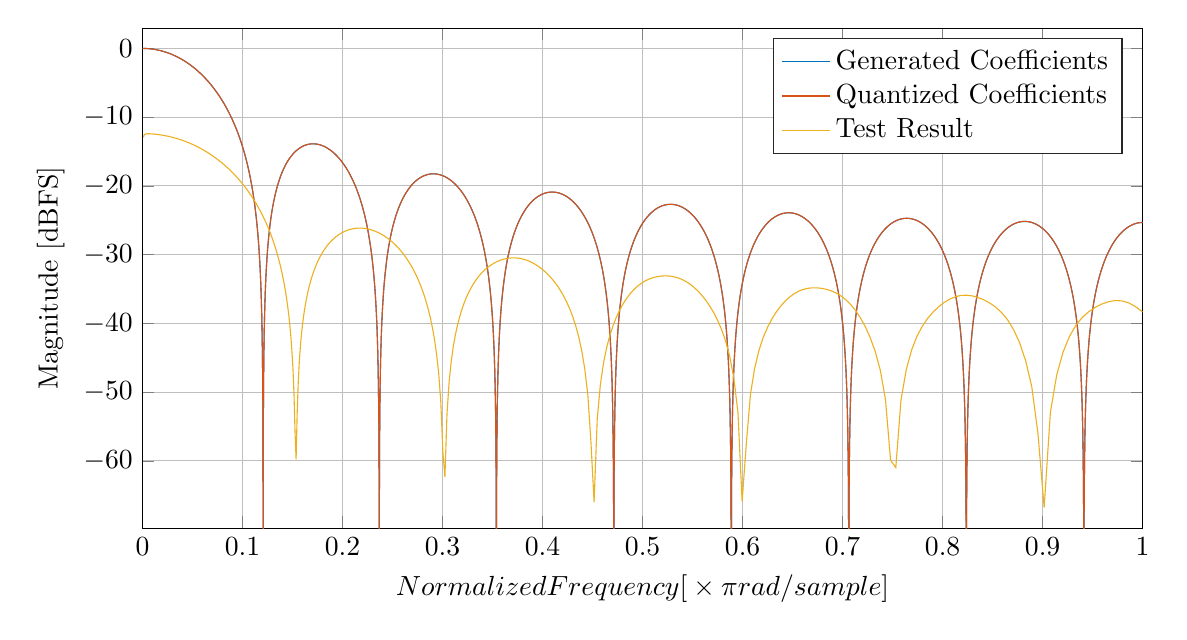
\begin{tikzpicture}

\begin{axis}[%
width=5.in,
height=2.5in,
at={(2.804in,1.205in)},
scale only axis,
unbounded coords=jump,
xmin=0,
xmax=0.9998779296875,
xlabel={$\text{Normalized Frequency [}\times\pi\text{ rad/sample]}$},
xmajorgrids,
ymin=-69.8016858010277,
ymax=2.94050574030787,
ylabel={Magnitude [dBFS]},
ymajorgrids,
axis background/.style={fill=white},
title style={font=\bfseries},
legend style={legend cell align=left,align=left,draw=white!15!black}
]

\addplot [color=mycolor1,solid,forget plot]
  table[row sep=crcr]{%
0	-3.41060513164848e-13\\
0.0001220703125	-1.48448838217519e-05\\
0.000244140625	-5.93795939494157e-05\\
0.0003662109375	-0.000133604309439761\\
0.00048828125	-0.000237519328550206\\
0.0006103515625	-0.000371125068454603\\
0.000732421875	-0.000534422065811668\\
0.0008544921875	-0.000727410976480769\\
0.0009765625	-0.000950092575465078\\
0.0010986328125	-0.00120246775730948\\
0.001220703125	-0.00148453753558897\\
0.0013427734375	-0.00179630304342027\\
0.00146484375	-0.00213776553312073\\
0.0015869140625	-0.00250892637649258\\
0.001708984375	-0.00290978706459555\\
0.0018310546875	-0.00334034920803106\\
0.001953125	-0.0038006145368854\\
0.0020751953125	-0.00429058490061607\\
0.002197265625	-0.00481026226822223\\
0.0023193359375	-0.00535964872841532\\
0.00244140625	-0.00593874648927795\\
0.0025634765625	-0.00654755787871864\\
0.002685546875	-0.00718608534424447\\
0.0028076171875	-0.00785433145318848\\
0.0029296875	-0.00855229889253906\\
0.0030517578125	-0.00927999046928107\\
0.003173828125	-0.0100374091101116\\
0.0032958984375	-0.0108245578618948\\
0.00341796875	-0.011641439891207\\
0.0035400390625	-0.0124880584850189\\
0.003662109375	-0.0133644170501839\\
0.0037841796875	-0.014270519113893\\
0.00390625	-0.015206368323561\\
0.0040283203125	-0.0161719684468835\\
0.004150390625	-0.0171673233720071\\
0.0042724609375	-0.0181924371076434\\
0.00439453125	-0.0192473137828983\\
0.0045166015625	-0.0203319576476133\\
0.004638671875	-0.0214463730724219\\
0.0047607421875	-0.0225905645485796\\
0.0048828125	-0.0237645366883612\\
0.0050048828125	-0.0249682942250615\\
0.005126953125	-0.0262018420128811\\
0.0052490234375	-0.0274651850273813\\
0.00537109375	-0.0287583283652566\\
0.0054931640625	-0.0300812772446193\\
0.005615234375	-0.031434037004999\\
0.0057373046875	-0.0328166131075136\\
0.005859375	-0.0342290111349257\\
0.0059814453125	-0.0356712367918703\\
0.006103515625	-0.0371432959047411\\
0.0062255859375	-0.038645194422088\\
0.00634765625	-0.0401769384143904\\
0.0064697265625	-0.0417385340744545\\
0.006591796875	-0.0433299877175273\\
0.0067138671875	-0.0449513057811828\\
0.0068359375	-0.04660249482572\\
0.0069580078125	-0.0482835615340491\\
0.007080078125	-0.0499945127120895\\
0.0072021484375	-0.0517353552885425\\
0.00732421875	-0.0535060963154592\\
0.0074462890625	-0.0553067429680709\\
0.007568359375	-0.057137302544902\\
0.0076904296875	-0.0589977824681682\\
0.0078125	-0.0608881902836629\\
0.0079345703125	-0.0628085336611548\\
0.008056640625	-0.0647588203942746\\
0.0081787109375	-0.0667390584008558\\
0.00830078125	-0.0687492557229916\\
0.0084228515625	-0.0707894205272055\\
0.008544921875	-0.0728595611046785\\
0.0086669921875	-0.0749596858713062\\
0.0087890625	-0.0770898033680396\\
0.0089111328125	-0.0792499222607717\\
0.009033203125	-0.081440051340735\\
0.0091552734375	-0.0836601995247293\\
0.00927734375	-0.085910375854894\\
0.0093994140625	-0.0881905894994475\\
0.009521484375	-0.0905008497524022\\
0.0096435546875	-0.0928411660340771\\
0.009765625	-0.0952115478909263\\
0.0098876953125	-0.0976120049961082\\
0.010009765625	-0.100042547149485\\
0.0101318359375	-0.102503184277793\\
0.01025390625	-0.104993926434815\\
0.0103759765625	-0.107514783801832\\
0.010498046875	-0.110065766687399\\
0.0106201171875	-0.112646885527909\\
0.0107421875	-0.115258150887712\\
0.0108642578125	-0.117899573459169\\
0.010986328125	-0.120571164063108\\
0.0111083984375	-0.123272933648764\\
0.01123046875	-0.126004893294294\\
0.0113525390625	-0.128767054206719\\
0.011474609375	-0.131559427722323\\
0.0115966796875	-0.13438202530682\\
0.01171875	-0.13723485855553\\
0.0118408203125	-0.140117939193829\\
0.011962890625	-0.143031279076979\\
0.0120849609375	-0.145974890190871\\
0.01220703125	-0.148948784651736\\
0.0123291015625	-0.151952974706774\\
0.012451171875	-0.154987472734319\\
0.0125732421875	-0.158052291244019\\
0.0126953125	-0.161147442876938\\
0.0128173828125	-0.164272940406249\\
0.012939453125	-0.167428796736942\\
0.0130615234375	-0.17061502490651\\
0.01318359375	-0.173831638085119\\
0.0133056640625	-0.177078649575606\\
0.013427734375	-0.180356072814106\\
0.0135498046875	-0.183663921370169\\
0.013671875	-0.187002208946865\\
0.0137939453125	-0.190370949381418\\
0.013916015625	-0.193770156645201\\
0.0140380859375	-0.197199844844079\\
0.01416015625	-0.200660028218806\\
0.0142822265625	-0.20415072114514\\
0.014404296875	-0.20767193813424\\
0.0145263671875	-0.211223693832949\\
0.0146484375	-0.214806003024137\\
0.0147705078125	-0.218418880626871\\
0.014892578125	-0.222062341696812\\
0.0150146484375	-0.225736401426445\\
0.01513671875	-0.229441075145587\\
0.0152587890625	-0.233176378321446\\
0.015380859375	-0.236942326559017\\
0.0155029296875	-0.240738935601485\\
0.015625	-0.244566221330558\\
0.0157470703125	-0.248424199766532\\
0.015869140625	-0.252312887068967\\
0.0159912109375	-0.256232299536748\\
0.01611328125	-0.26018245360865\\
0.0162353515625	-0.26416336586351\\
0.016357421875	-0.268175053020514\\
0.0164794921875	-0.272217531939702\\
0.0166015625	-0.276290819622318\\
0.0167236328125	-0.280394933211028\\
0.016845703125	-0.284529889990324\\
0.0169677734375	-0.288695707386921\\
0.01708984375	-0.29289240297004\\
0.0172119140625	-0.297119994451862\\
0.017333984375	-0.301378499687814\\
0.0174560546875	-0.305667936677082\\
0.017578125	-0.309988323562777\\
0.0177001953125	-0.314339678632393\\
0.017822265625	-0.318722020318262\\
0.0179443359375	-0.323135367197949\\
0.01806640625	-0.327579737994427\\
0.0181884765625	-0.33205515157664\\
0.018310546875	-0.33656162696002\\
0.0184326171875	-0.34109918330654\\
0.0185546875	-0.345667839925397\\
0.0186767578125	-0.350267616273356\\
0.018798828125	-0.354898531955087\\
0.0189208984375	-0.359560606723619\\
0.01904296875	-0.364253860480744\\
0.0191650390625	-0.368978313277466\\
0.019287109375	-0.373733985314402\\
0.0194091796875	-0.378520896942291\\
0.01953125	-0.383339068662167\\
0.0196533203125	-0.388188521126096\\
0.019775390625	-0.393069275137464\\
0.0198974609375	-0.397981351651424\\
0.02001953125	-0.402924771775361\\
0.0201416015625	-0.407899556769337\\
0.020263671875	-0.412905728046496\\
0.0203857421875	-0.417943307173687\\
0.0205078125	-0.423012315871688\\
0.0206298828125	-0.428112776015837\\
0.020751953125	-0.433244709636369\\
0.0208740234375	-0.438408138919101\\
0.02099609375	-0.443603086205655\\
0.0211181640625	-0.44882957399409\\
0.021240234375	-0.454087624939461\\
0.0213623046875	-0.459377261853945\\
0.021484375	-0.464698507707794\\
0.0216064453125	-0.470051385629631\\
0.021728515625	-0.475435918906783\\
0.0218505859375	-0.480852130986023\\
0.02197265625	-0.486300045473968\\
0.0220947265625	-0.491779686137761\\
0.022216796875	-0.497291076905242\\
0.0223388671875	-0.502834241865799\\
0.0224609375	-0.508409205270652\\
0.0225830078125	-0.514015991533711\\
0.022705078125	-0.519654625231567\\
0.0228271484375	-0.525325131104751\\
0.02294921875	-0.5310275340575\\
0.0230712890625	-0.536761859158901\\
0.023193359375	-0.542528131643223\\
0.0233154296875	-0.548326376910438\\
0.0234375	-0.554156620526783\\
0.0235595703125	-0.560018888225386\\
0.023681640625	-0.565913205906838\\
0.0238037109375	-0.571839599639702\\
0.02392578125	-0.57779809566108\\
0.0240478515625	-0.583788720377356\\
0.024169921875	-0.589811500364533\\
0.0242919921875	-0.595866462369145\\
0.0244140625	-0.601953633308426\\
0.0245361328125	-0.608073040271279\\
0.024658203125	-0.61422471051884\\
0.0247802734375	-0.620408671484881\\
0.02490234375	-0.626624950776488\\
0.0250244140625	-0.632873576174973\\
0.025146484375	-0.639154575636041\\
0.0252685546875	-0.645467977290764\\
0.025390625	-0.651813809446082\\
0.0255126953125	-0.658192100585381\\
0.025634765625	-0.66460287936934\\
0.0257568359375	-0.671046174636388\\
0.02587890625	-0.67752201540344\\
0.0260009765625	-0.684030430866528\\
0.026123046875	-0.690571450401478\\
0.0262451171875	-0.697145103564708\\
0.0263671875	-0.703751420093624\\
0.0264892578125	-0.710390429907477\\
0.026611328125	-0.717062163108153\\
0.0267333984375	-0.723766649980689\\
0.02685546875	-0.730503920993897\\
0.0269775390625	-0.737274006801385\\
0.027099609375	-0.744076938242017\\
0.0272216796875	-0.750912746340589\\
0.02734375	-0.757781462308742\\
0.0274658203125	-0.76468311754553\\
0.027587890625	-0.77161774363833\\
0.0277099609375	-0.778585372363239\\
0.02783203125	-0.785586035686265\\
0.0279541015625	-0.792619765763732\\
0.028076171875	-0.799686594943012\\
0.0281982421875	-0.806786555763722\\
0.0283203125	-0.813919680957838\\
0.0284423828125	-0.821086003451057\\
0.028564453125	-0.828285556363255\\
0.0286865234375	-0.835518373009279\\
0.02880859375	-0.842784486899802\\
0.0289306640625	-0.850083931742233\\
0.029052734375	-0.857416741441227\\
0.0291748046875	-0.864782950099766\\
0.029296875	-0.87218259201984\\
0.0294189453125	-0.879615701703301\\
0.029541015625	-0.887082313852602\\
0.0296630859375	-0.894582463371819\\
0.02978515625	-0.902116185367277\\
0.0299072265625	-0.909683515148515\\
0.030029296875	-0.9172844882292\\
0.0301513671875	-0.924919140327802\\
0.0302734375	-0.932587507368567\\
0.0303955078125	-0.940289625482364\\
0.030517578125	-0.948025531007602\\
0.0306396484375	-0.955795260491129\\
0.03076171875	-0.963598850688982\\
0.0308837890625	-0.971436338567457\\
0.031005859375	-0.979307761303858\\
0.0311279296875	-0.987213156287567\\
0.03125	-0.995152561120847\\
0.0313720703125	-1.00312601361975\\
0.031494140625	-1.01113355181525\\
0.0316162109375	-1.01917521395387\\
0.03173828125	-1.02725103849889\\
0.0318603515625	-1.03536106413117\\
0.031982421875	-1.04350532975013\\
0.0321044921875	-1.0516838744748\\
0.0322265625	-1.05989673764464\\
0.0323486328125	-1.06814395882071\\
0.032470703125	-1.07642557778644\\
0.0325927734375	-1.08474163454883\\
0.03271484375	-1.09309216933946\\
0.0328369140625	-1.10147722261524\\
0.032958984375	-1.10989683505977\\
0.0330810546875	-1.1183510475841\\
0.033203125	-1.12683990132797\\
0.0333251953125	-1.13536343766066\\
0.033447265625	-1.14392169818228\\
0.0335693359375	-1.1525147247246\\
0.03369140625	-1.1611425593523\\
0.0338134765625	-1.16980524436389\\
0.033935546875	-1.1785028222929\\
0.0340576171875	-1.18723533590895\\
0.0341796875	-1.19600282821887\\
0.0343017578125	-1.20480534246781\\
0.034423828125	-1.21364292214025\\
0.0345458984375	-1.2225156109613\\
0.03466796875	-1.23142345289773\\
0.0347900390625	-1.24036649215913\\
0.034912109375	-1.24934477319914\\
0.0350341796875	-1.25835834071643\\
0.03515625	-1.26740723965617\\
0.0352783203125	-1.27649151521081\\
0.035400390625	-1.28561121282172\\
0.0355224609375	-1.29476637817999\\
0.03564453125	-1.30395705722788\\
0.0357666015625	-1.31318329615999\\
0.035888671875	-1.32244514142451\\
0.0360107421875	-1.33174263972427\\
0.0361328125	-1.3410758380183\\
0.0362548828125	-1.35044478352279\\
0.036376953125	-1.35984952371251\\
0.0364990234375	-1.36929010632218\\
0.03662109375	-1.37876657934748\\
0.0367431640625	-1.3882789910466\\
0.036865234375	-1.39782738994137\\
0.0369873046875	-1.40741182481878\\
0.037109375	-1.41703234473209\\
0.0372314453125	-1.42668899900224\\
0.037353515625	-1.4363818372193\\
0.0374755859375	-1.44611090924366\\
0.03759765625	-1.45587626520751\\
0.0377197265625	-1.46567795551618\\
0.037841796875	-1.47551603084963\\
0.0379638671875	-1.4853905421636\\
0.0380859375	-1.49530154069134\\
0.0382080078125	-1.50524907794471\\
0.038330078125	-1.5152332057159\\
0.0384521484375	-1.52525397607872\\
0.03857421875	-1.53531144139009\\
0.0386962890625	-1.54540565429147\\
0.038818359375	-1.55553666771044\\
0.0389404296875	-1.56570453486205\\
0.0390625	-1.57590930925039\\
0.0391845703125	-1.5861510446702\\
0.039306640625	-1.59642979520828\\
0.0394287109375	-1.60674561524496\\
0.03955078125	-1.61709855945583\\
0.0396728515625	-1.62748868281324\\
0.039794921875	-1.63791604058775\\
0.0399169921875	-1.64838068834996\\
0.0400390625	-1.65888268197182\\
0.0401611328125	-1.6694220776285\\
0.040283203125	-1.6799989317999\\
0.0404052734375	-1.69061330127221\\
0.04052734375	-1.70126524313969\\
0.0406494140625	-1.71195481480635\\
0.040771484375	-1.72268207398747\\
0.0408935546875	-1.73344707871149\\
0.041015625	-1.74424988732159\\
0.0411376953125	-1.75509055847726\\
0.041259765625	-1.76596915115653\\
0.0413818359375	-1.77688572465712\\
0.04150390625	-1.78784033859853\\
0.0416259765625	-1.79883305292384\\
0.041748046875	-1.80986392790135\\
0.0418701171875	-1.82093302412642\\
0.0419921875	-1.83204040252332\\
0.0421142578125	-1.84318612434714\\
0.042236328125	-1.85437025118546\\
0.0423583984375	-1.8655928449603\\
0.04248046875	-1.87685396793\\
0.0426025390625	-1.88815368269115\\
0.042724609375	-1.89949205218051\\
0.0428466796875	-1.91086913967666\\
0.04296875	-1.92228500880231\\
0.0430908203125	-1.93373972352617\\
0.043212890625	-1.94523334816472\\
0.0433349609375	-1.95676594738438\\
0.04345703125	-1.9683375862034\\
0.0435791015625	-1.97994832999399\\
0.043701171875	-1.99159824448429\\
0.0438232421875	-2.00328739576042\\
0.0439453125	-2.01501585026853\\
0.0440673828125	-2.02678367481701\\
0.044189453125	-2.03859093657832\\
0.0443115234375	-2.05043770309146\\
0.04443359375	-2.06232404226387\\
0.0445556640625	-2.07425002237363\\
0.044677734375	-2.08621571207158\\
0.0447998046875	-2.09822118038375\\
0.044921875	-2.11026649671328\\
0.0450439453125	-2.12235173084269\\
0.045166015625	-2.13447695293638\\
0.0452880859375	-2.14664223354259\\
0.04541015625	-2.15884764359583\\
0.0455322265625	-2.17109325441913\\
0.045654296875	-2.18337913772643\\
0.0457763671875	-2.19570536562492\\
0.0458984375	-2.20807201061717\\
0.0460205078125	-2.22047914560397\\
0.046142578125	-2.23292684388616\\
0.0462646484375	-2.24541517916754\\
0.04638671875	-2.25794422555708\\
0.0465087890625	-2.2705140575714\\
0.046630859375	-2.28312475013723\\
0.0467529296875	-2.29577637859398\\
0.046875	-2.3084690186962\\
0.0469970703125	-2.32120274661622\\
0.047119140625	-2.33397763894658\\
0.0472412109375	-2.34679377270277\\
0.04736328125	-2.35965122532559\\
0.0474853515625	-2.37255007468411\\
0.047607421875	-2.38549039907815\\
0.0477294921875	-2.3984722772409\\
0.0478515625	-2.41149578834171\\
0.0479736328125	-2.42456101198877\\
0.048095703125	-2.437668028232\\
0.0482177734375	-2.45081691756553\\
0.04833984375	-2.46400776093083\\
0.0484619140625	-2.47724063971913\\
0.048583984375	-2.49051563577473\\
0.0487060546875	-2.50383283139752\\
0.048828125	-2.51719230934594\\
0.0489501953125	-2.53059415283997\\
0.049072265625	-2.54403844556407\\
0.0491943359375	-2.5575252716701\\
0.04931640625	-2.57105471578029\\
0.0494384765625	-2.58462686299032\\
0.049560546875	-2.59824179887227\\
0.0496826171875	-2.61189960947786\\
0.0498046875	-2.62560038134137\\
0.0499267578125	-2.63934420148291\\
0.050048828125	-2.65313115741139\\
0.0501708984375	-2.66696133712804\\
0.05029296875	-2.68083482912914\\
0.0504150390625	-2.69475172240959\\
0.050537109375	-2.70871210646624\\
0.0506591796875	-2.72271607130079\\
0.05078125	-2.73676370742356\\
0.0509033203125	-2.7508551058566\\
0.051025390625	-2.76499035813714\\
0.0511474609375	-2.77916955632082\\
0.05126953125	-2.79339279298546\\
0.0513916015625	-2.80766016123437\\
0.051513671875	-2.82197175469969\\
0.0516357421875	-2.8363276675463\\
0.0517578125	-2.85072799447505\\
0.0518798828125	-2.86517283072646\\
0.052001953125	-2.87966227208449\\
0.0521240234375	-2.89419641487996\\
0.05224609375	-2.90877535599446\\
0.0523681640625	-2.923399192864\\
0.052490234375	-2.93806802348269\\
0.0526123046875	-2.95278194640673\\
0.052734375	-2.96754106075809\\
0.0528564453125	-2.98234546622837\\
0.052978515625	-2.99719526308292\\
0.0531005859375	-3.01209055216435\\
0.05322265625	-3.02703143489708\\
0.0533447265625	-3.04201801329077\\
0.053466796875	-3.05705038994483\\
0.0535888671875	-3.07212866805219\\
0.0537109375	-3.08725295140368\\
0.0538330078125	-3.10242334439192\\
0.053955078125	-3.11763995201574\\
0.0540771484375	-3.13290287988428\\
0.05419921875	-3.14821223422138\\
0.0543212890625	-3.1635681218699\\
0.054443359375	-3.17897065029581\\
0.0545654296875	-3.194419927593\\
0.0546875	-3.20991606248737\\
0.0548095703125	-3.2254591643416\\
0.054931640625	-3.24104934315937\\
0.0550537109375	-3.25668670959016\\
0.05517578125	-3.27237137493381\\
0.0552978515625	-3.28810345114505\\
0.055419921875	-3.30388305083835\\
0.0555419921875	-3.31971028729254\\
0.0556640625	-3.3355852744557\\
0.0557861328125	-3.3515081269498\\
0.055908203125	-3.36747896007591\\
0.0560302734375	-3.38349788981873\\
0.05615234375	-3.3995650328518\\
0.0562744140625	-3.41568050654251\\
0.056396484375	-3.43184442895711\\
0.0565185546875	-3.44805691886569\\
0.056640625	-3.46431809574767\\
0.0567626953125	-3.48062807979665\\
0.056884765625	-3.49698699192584\\
0.0570068359375	-3.51339495377346\\
0.05712890625	-3.52985208770798\\
0.0572509765625	-3.54635851683344\\
0.057373046875	-3.56291436499521\\
0.0574951171875	-3.5795197567852\\
0.0576171875	-3.59617481754765\\
0.0577392578125	-3.61287967338455\\
0.057861328125	-3.62963445116162\\
0.0579833984375	-3.6464392785137\\
0.05810546875	-3.66329428385086\\
0.0582275390625	-3.68019959636399\\
0.058349609375	-3.69715534603091\\
0.0584716796875	-3.71416166362224\\
0.05859375	-3.73121868070734\\
0.0587158203125	-3.74832652966069\\
0.058837890625	-3.76548534366765\\
0.0589599609375	-3.7826952567309\\
0.05908203125	-3.79995640367679\\
0.0592041015625	-3.81726892016133\\
0.059326171875	-3.83463294267705\\
0.0594482421875	-3.85204860855896\\
0.0595703125	-3.86951605599143\\
0.0596923828125	-3.88703542401475\\
0.059814453125	-3.90460685253163\\
0.0599365234375	-3.92223048231392\\
0.06005859375	-3.93990645500958\\
0.0601806640625	-3.95763491314938\\
0.060302734375	-3.97541600015387\\
0.0604248046875	-3.99324986034048\\
0.060546875	-4.0111366389304\\
0.0606689453125	-4.02907648205581\\
0.060791015625	-4.04706953676725\\
0.0609130859375	-4.06511595104053\\
0.06103515625	-4.08321587378458\\
0.0611572265625	-4.10136945484845\\
0.061279296875	-4.11957684502909\\
0.0614013671875	-4.13783819607886\\
0.0615234375	-4.15615366071319\\
0.0616455078125	-4.17452339261831\\
0.061767578125	-4.19294754645932\\
0.0618896484375	-4.2114262778876\\
0.06201171875	-4.22995974354933\\
0.0621337890625	-4.24854810109332\\
0.062255859375	-4.26719150917916\\
0.0623779296875	-4.28589012748552\\
0.0625	-4.30464411671846\\
0.0626220703125	-4.32345363861998\\
0.062744140625	-4.34231885597632\\
0.0628662109375	-4.36123993262669\\
0.06298828125	-4.38021703347204\\
0.0631103515625	-4.39925032448372\\
0.063232421875	-4.41833997271226\\
0.0633544921875	-4.43748614629669\\
0.0634765625	-4.45668901447328\\
0.0635986328125	-4.47594874758488\\
0.063720703125	-4.49526551709016\\
0.0638427734375	-4.51463949557285\\
0.06396484375	-4.53407085675144\\
0.0640869140625	-4.55355977548857\\
0.064208984375	-4.57310642780078\\
0.0643310546875	-4.59271099086828\\
0.064453125	-4.61237364304475\\
0.0645751953125	-4.6320945638675\\
0.064697265625	-4.65187393406745\\
0.0648193359375	-4.67171193557942\\
0.06494140625	-4.69160875155222\\
0.0650634765625	-4.71156456635953\\
0.065185546875	-4.73157956561005\\
0.0653076171875	-4.75165393615833\\
0.0654296875	-4.77178786611557\\
0.0655517578125	-4.7919815448605\\
0.065673828125	-4.81223516305039\\
0.0657958984375	-4.83254891263226\\
0.06591796875	-4.85292298685414\\
0.0660400390625	-4.87335758027632\\
0.066162109375	-4.89385288878316\\
0.0662841796875	-4.91440910959454\\
0.06640625	-4.93502644127773\\
0.0665283203125	-4.9557050837592\\
0.066650390625	-4.97644523833691\\
0.0667724609375	-4.99724710769232\\
0.06689453125	-5.01811089590274\\
0.0670166015625	-5.03903680845377\\
0.067138671875	-5.06002505225217\\
0.0672607421875	-5.08107583563827\\
0.0673828125	-5.10218936839914\\
0.0675048828125	-5.12336586178139\\
0.067626953125	-5.14460552850477\\
0.0677490234375	-5.1659085827751\\
0.06787109375	-5.18727524029799\\
0.0679931640625	-5.20870571829255\\
0.068115234375	-5.23020023550521\\
0.0682373046875	-5.25175901222349\\
0.068359375	-5.27338227029043\\
0.0684814453125	-5.29507023311885\\
0.068603515625	-5.31682312570564\\
0.0687255859375	-5.33864117464668\\
0.06884765625	-5.36052460815154\\
0.0689697265625	-5.38247365605844\\
0.069091796875	-5.40448854984948\\
0.0692138671875	-5.42656952266611\\
0.0693359375	-5.44871680932448\\
0.0694580078125	-5.47093064633134\\
0.069580078125	-5.49321127189978\\
0.0697021484375	-5.51555892596554\\
0.06982421875	-5.53797385020317\\
0.0699462890625	-5.56045628804264\\
0.070068359375	-5.58300648468588\\
0.0701904296875	-5.60562468712379\\
0.0703125	-5.62831114415343\\
0.0704345703125	-5.65106610639509\\
0.070556640625	-5.67388982631007\\
0.0706787109375	-5.69678255821816\\
0.07080078125	-5.71974455831599\\
0.0709228515625	-5.74277608469464\\
0.071044921875	-5.76587739735862\\
0.0711669921875	-5.78904875824412\\
0.0712890625	-5.8122904312379\\
0.0714111328125	-5.83560268219657\\
0.071533203125	-5.8589857789658\\
0.0716552734375	-5.88243999139979\\
0.07177734375	-5.90596559138135\\
0.0718994140625	-5.92956285284163\\
0.072021484375	-5.95323205178062\\
0.0721435546875	-5.9769734662878\\
0.072265625	-6.00078737656281\\
0.0723876953125	-6.02467406493656\\
0.072509765625	-6.04863381589269\\
0.0726318359375	-6.07266691608896\\
0.07275390625	-6.09677365437955\\
0.0728759765625	-6.1209543218369\\
0.072998046875	-6.14520921177433\\
0.0731201171875	-6.16953861976867\\
0.0732421875	-6.1939428436836\\
0.0733642578125	-6.21842218369261\\
0.073486328125	-6.24297694230296\\
0.0736083984375	-6.26760742437949\\
0.07373046875	-6.2923139371689\\
0.0738525390625	-6.3170967903244\\
0.073974609375	-6.34195629593052\\
0.0740966796875	-6.36689276852843\\
0.07421875	-6.39190652514145\\
0.0743408203125	-6.41699788530099\\
0.074462890625	-6.4421671710727\\
0.0745849609375	-6.46741470708326\\
0.07470703125	-6.49274082054711\\
0.0748291015625	-6.51814584129386\\
0.074951171875	-6.54363010179594\\
0.0750732421875	-6.56919393719659\\
0.0751953125	-6.59483768533835\\
0.0753173828125	-6.62056168679192\\
0.075439453125	-6.64636628488518\\
0.0755615234375	-6.6722518257327\\
0.07568359375	-6.69821865826617\\
0.0758056640625	-6.72426713426427\\
0.075927734375	-6.75039760838371\\
0.0760498046875	-6.77661043819052\\
0.076171875	-6.80290598419151\\
0.0762939453125	-6.82928460986653\\
0.076416015625	-6.85574668170102\\
0.0765380859375	-6.88229256921881\\
0.07666015625	-6.90892264501571\\
0.0767822265625	-6.9356372847933\\
0.076904296875	-6.96243686739354\\
0.0770263671875	-6.98932177483334\\
0.0771484375	-7.01629239234001\\
0.0772705078125	-7.04334910838725\\
0.077392578125	-7.07049231473133\\
0.0775146484375	-7.09772240644799\\
0.07763671875	-7.12503978196986\\
0.0777587890625	-7.15244484312439\\
0.077880859375	-7.17993799517228\\
0.0780029296875	-7.20751964684644\\
0.078125	-7.23519021039169\\
0.0782470703125	-7.26295010160482\\
0.078369140625	-7.2907997398753\\
0.0784912109375	-7.31873954822669\\
0.07861328125	-7.34676995335826\\
0.0787353515625	-7.37489138568799\\
0.078857421875	-7.40310427939528\\
0.0789794921875	-7.43140907246482\\
0.0791015625	-7.45980620673129\\
0.0792236328125	-7.48829612792395\\
0.079345703125	-7.51687928571283\\
0.0794677734375	-7.54555613375476\\
0.07958984375	-7.57432712974077\\
0.0797119140625	-7.60319273544377\\
0.079833984375	-7.63215341676704\\
0.0799560546875	-7.66120964379354\\
0.080078125	-7.69036189083573\\
0.0802001953125	-7.71961063648666\\
0.080322265625	-7.7489563636712\\
0.0804443359375	-7.77839955969824\\
0.08056640625	-7.80794071631408\\
0.0806884765625	-7.83758032975618\\
0.080810546875	-7.8673189008079\\
0.0809326171875	-7.89715693485385\\
0.0810546875	-7.92709494193673\\
0.0811767578125	-7.95713343681433\\
0.081298828125	-7.98727293901766\\
0.0814208984375	-8.01751397291036\\
0.08154296875	-8.04785706774834\\
0.0816650390625	-8.07830275774086\\
0.081787109375	-8.10885158211266\\
0.0819091796875	-8.13950408516638\\
0.08203125	-8.1702608163468\\
0.0821533203125	-8.20112233030574\\
0.082275390625	-8.23208918696764\\
0.0823974609375	-8.26316195159683\\
0.08251953125	-8.29434119486547\\
0.0826416015625	-8.32562749292271\\
0.082763671875	-8.35702142746487\\
0.0828857421875	-8.38852358580687\\
0.0830078125	-8.42013456095486\\
0.0831298828125	-8.45185495167965\\
0.083251953125	-8.48368536259198\\
0.0833740234375	-8.51562640421849\\
0.08349609375	-8.54767869307904\\
0.0836181640625	-8.57984285176553\\
0.083740234375	-8.61211950902191\\
0.0838623046875	-8.64450929982519\\
0.083984375	-8.67701286546855\\
0.0841064453125	-8.70963085364485\\
0.084228515625	-8.74236391853259\\
0.0843505859375	-8.77521272088239\\
0.08447265625	-8.80817792810552\\
0.0845947265625	-8.84126021436373\\
0.084716796875	-8.87446026066056\\
0.0848388671875	-8.90777875493433\\
0.0849609375	-8.94121639215257\\
0.0850830078125	-8.97477387440824\\
0.085205078125	-9.0084519110174\\
0.0853271484375	-9.04225121861884\\
0.08544921875	-9.07617252127528\\
0.0855712890625	-9.11021655057601\\
0.085693359375	-9.14438404574213\\
0.0858154296875	-9.17867575373282\\
0.0859375	-9.21309242935399\\
0.0860595703125	-9.24763483536839\\
0.086181640625	-9.28230374260835\\
0.0863037109375	-9.31709993008974\\
0.08642578125	-9.3520241851287\\
0.0865478515625	-9.38707730345965\\
0.086669921875	-9.42226008935637\\
0.0867919921875	-9.45757335575439\\
0.0869140625	-9.49301792437609\\
0.0870361328125	-9.52859462585798\\
0.087158203125	-9.56430429988023\\
0.0872802734375	-9.6001477952986\\
0.08740234375	-9.6361259702789\\
0.0875244140625	-9.67223969243361\\
0.087646484375	-9.7084898389615\\
0.0877685546875	-9.7448772967893\\
0.087890625	-9.78140296271658\\
0.0880126953125	-9.81806774356284\\
0.088134765625	-9.85487255631773\\
0.0882568359375	-9.89181832829377\\
0.08837890625	-9.92890599728236\\
0.0885009765625	-9.96613651171225\\
0.088623046875	-10.0035108308115\\
0.0887451171875	-10.0410299247724\\
0.0888671875	-10.0786947749193\\
0.0889892578125	-10.1165063738798\\
0.089111328125	-10.1544657257598\\
0.0892333984375	-10.1925738463211\\
0.08935546875	-10.2308317631627\\
0.0894775390625	-10.2692405159063\\
0.089599609375	-10.3078011563845\\
0.0897216796875	-10.3465147488332\\
0.08984375	-10.3853823700882\\
0.0899658203125	-10.4244051097846\\
0.090087890625	-10.4635840705615\\
0.0902099609375	-10.5029203682697\\
0.09033203125	-10.5424151321843\\
0.0904541015625	-10.5820695052211\\
0.090576171875	-10.621884644158\\
0.0906982421875	-10.6618617198604\\
0.0908203125	-10.702001917511\\
0.0909423828125	-10.7423064368454\\
0.091064453125	-10.782776492391\\
0.0911865234375	-10.8234133137126\\
0.09130859375	-10.8642181456613\\
0.0914306640625	-10.9051922486302\\
0.091552734375	-10.9463368988144\\
0.0916748046875	-10.987653388477\\
0.091796875	-11.0291430262205\\
0.0919189453125	-11.070807137264\\
0.092041015625	-11.1126470637265\\
0.0921630859375	-11.1546641649159\\
0.09228515625	-11.1968598176247\\
0.0924072265625	-11.2392354164318\\
0.092529296875	-11.2817923740104\\
0.0926513671875	-11.3245321214439\\
0.0927734375	-11.3674561085473\\
0.0928955078125	-11.4105658041967\\
0.093017578125	-11.4538626966652\\
0.0931396484375	-11.497348293967\\
0.09326171875	-11.5410241242092\\
0.0933837890625	-11.5848917359505\\
0.093505859375	-11.628952698569\\
0.0936279296875	-11.6732086026381\\
0.09375	-11.7176610603104\\
0.0938720703125	-11.7623117057109\\
0.093994140625	-11.8071621953392\\
0.0941162109375	-11.8522142084806\\
0.09423828125	-11.8974694476266\\
0.0943603515625	-11.9429296389062\\
0.094482421875	-11.9885965325258\\
0.0946044921875	-12.0344719032203\\
0.0947265625	-12.0805575507151\\
0.0948486328125	-12.1268553001978\\
0.094970703125	-12.1733670028026\\
0.0950927734375	-12.2200945361053\\
0.09521484375	-12.26703980463\\
0.0953369140625	-12.3142047403695\\
0.095458984375	-12.3615913033163\\
0.0955810546875	-12.4092014820079\\
0.095703125	-12.457037294085\\
0.0958251953125	-12.5051007868637\\
0.095947265625	-12.5533940379212\\
0.0960693359375	-12.601919155697\\
0.09619140625	-12.6506782801081\\
0.0963134765625	-12.6996735831801\\
0.096435546875	-12.748907269695\\
0.0965576171875	-12.7983815778535\\
0.0966796875	-12.8480987799563\\
0.0968017578125	-12.898061183101\\
0.096923828125	-12.9482711298987\\
0.0970458984375	-12.9987309992075\\
0.09716796875	-13.0494432068859\\
0.0972900390625	-13.1004102065663\\
0.097412109375	-13.1516344904475\\
0.0975341796875	-13.2031185901096\\
0.09765625	-13.2548650773497\\
0.0977783203125	-13.3068765650401\\
0.097900390625	-13.359155708009\\
0.0980224609375	-13.4117052039465\\
0.09814453125	-13.4645277943333\\
0.0982666015625	-13.517626265396\\
0.098388671875	-13.5710034490879\\
0.0985107421875	-13.6246622240978\\
0.0986328125	-13.6786055168853\\
0.0987548828125	-13.7328363027463\\
0.098876953125	-13.7873576069076\\
0.0989990234375	-13.8421725056531\\
0.09912109375	-13.8972841274809\\
0.0992431640625	-13.9526956542945\\
0.099365234375	-14.0084103226273\\
0.0994873046875	-14.0644314249029\\
0.099609375	-14.120762310732\\
0.0997314453125	-14.1774063882469\\
0.099853515625	-14.2343671254754\\
0.0999755859375	-14.2916480517549\\
0.10009765625	-14.3492527591891\\
0.1002197265625	-14.4071849041481\\
0.100341796875	-14.4654482088128\\
0.1004638671875	-14.5240464627673\\
0.1005859375	-14.5829835246388\\
0.1007080078125	-14.642263323788\\
0.100830078125	-14.7018898620519\\
0.1009521484375	-14.76186721554\\
0.10107421875	-14.822199536487\\
0.1011962890625	-14.8828910551638\\
0.101318359375	-14.943946081848\\
0.1014404296875	-15.0053690088582\\
0.1015625	-15.0671643126525\\
0.1016845703125	-15.1293365559949\\
0.101806640625	-15.1918903901922\\
0.1019287109375	-15.254830557403\\
0.10205078125	-15.3181618930233\\
0.1021728515625	-15.3818893281512\\
0.102294921875	-15.4460178921323\\
0.1024169921875	-15.5105527151914\\
0.1025390625	-15.5754990311532\\
0.1026611328125	-15.6408621802543\\
0.102783203125	-15.7066476120518\\
0.1029052734375	-15.7728608884325\\
0.10302734375	-15.8395076867258\\
0.1031494140625	-15.9065938029252\\
0.103271484375	-15.9741251550233\\
0.1033935546875	-16.0421077864646\\
0.103515625	-16.1105478697216\\
0.1036376953125	-16.1794517099991\\
0.103759765625	-16.2488257490725\\
0.1038818359375	-16.3186765692657\\
0.10400390625	-16.3890108975751\\
0.1041259765625	-16.4598356099467\\
0.104248046875	-16.5311577357105\\
0.1043701171875	-16.6029844621838\\
0.1044921875	-16.6753231394464\\
0.1046142578125	-16.7481812852992\\
0.104736328125	-16.8215665904115\\
0.1048583984375	-16.8954869236691\\
0.10498046875	-16.9699503377294\\
0.1051025390625	-17.0449650747959\\
0.105224609375	-17.1205395726203\\
0.1053466796875	-17.1966824707448\\
0.10546875	-17.2734026169954\\
0.1055908203125	-17.3507090742384\\
0.105712890625	-17.4286111274132\\
0.1058349609375	-17.5071182908552\\
0.10595703125	-17.5862403159231\\
0.1060791015625	-17.6659871989456\\
0.106201171875	-17.7463691895042\\
0.1063232421875	-17.8273967990696\\
0.1064453125	-17.9090808100085\\
0.1065673828125	-17.9914322849817\\
0.106689453125	-18.0744625767536\\
0.1068115234375	-18.1581833384337\\
0.10693359375	-18.2426065341751\\
0.1070556640625	-18.3277444503536\\
0.107177734375	-18.413609707253\\
0.1072998046875	-18.5002152712856\\
0.107421875	-18.5875744677771\\
0.1075439453125	-18.6757009943467\\
0.107666015625	-18.7646089349174\\
0.1077880859375	-18.8543127743914\\
0.10791015625	-18.9448274140288\\
0.1080322265625	-19.0361681875714\\
0.108154296875	-19.1283508781547\\
0.1082763671875	-19.2213917360538\\
0.1083984375	-19.3153074973156\\
0.1085205078125	-19.4101154033285\\
0.108642578125	-19.5058332213875\\
0.1087646484375	-19.6024792663171\\
0.10888671875	-19.7000724232166\\
0.1090087890625	-19.7986321713988\\
0.109130859375	-19.8981786095988\\
0.1092529296875	-19.998732482534\\
0.109375	-20.1003152089026\\
0.1094970703125	-20.2029489109164\\
0.109619140625	-20.3066564454691\\
0.1097412109375	-20.41146143705\\
0.10986328125	-20.5173883125219\\
0.1099853515625	-20.6244623378915\\
0.110107421875	-20.7327096572108\\
0.1102294921875	-20.8421573337585\\
0.1103515625	-20.9528333936661\\
0.1104736328125	-21.064766872162\\
0.110595703125	-21.1779878626259\\
0.1107177734375	-21.2925275686616\\
0.11083984375	-21.4084183594128\\
0.1109619140625	-21.5256938283671\\
0.111083984375	-21.6443888559168\\
0.1112060546875	-21.7645396759669\\
0.111328125	-21.8861839469097\\
0.1114501953125	-22.0093608273132\\
0.111572265625	-22.1341110567047\\
0.1116943359375	-22.2604770418665\\
0.11181640625	-22.3885029491013\\
0.1119384765625	-22.5182348029701\\
0.112060546875	-22.6497205920543\\
0.1121826171875	-22.7830103823518\\
0.1123046875	-22.9181564389772\\
0.1124267578125	-23.055213356906\\
0.112548828125	-23.1942382015827\\
0.1126708984375	-23.3352906602994\\
0.11279296875	-23.4784332053494\\
0.1129150390625	-23.6237312700731\\
0.113037109375	-23.7712534390379\\
0.1131591796875	-23.9210716537373\\
0.11328125	-24.0732614353511\\
0.1134033203125	-24.227902126298\\
0.113525390625	-24.3850771525115\\
0.1136474609375	-24.5448743086118\\
0.11376953125	-24.7073860684158\\
0.1138916015625	-24.8727099235334\\
0.114013671875	-25.0409487531571\\
0.1141357421875	-25.2122112285567\\
0.1142578125	-25.3866122562633\\
0.1143798828125	-25.5642734644704\\
0.114501953125	-25.7453237378081\\
0.1146240234375	-25.9298998063834\\
0.11474609375	-26.1181468958295\\
0.1148681640625	-26.3102194461089\\
0.114990234375	-26.5062819079845\\
0.1151123046875	-26.7065096274526\\
0.115234375	-26.9110898300594\\
0.1153564453125	-27.1202227189494\\
0.115478515625	-27.3341227027914\\
0.1156005859375	-27.5530197724606\\
0.11572265625	-27.7771610486429\\
0.1158447265625	-28.0068125264752\\
0.115966796875	-28.2422610481126\\
0.1160888671875	-28.4838165399171\\
0.1162109375	-28.7318145580441\\
0.1163330078125	-28.9866191948908\\
0.116455078125	-29.2486264095908\\
0.1165771484375	-29.5182678590314\\
0.11669921875	-29.796015322465\\
0.1168212890625	-30.0823858336217\\
0.116943359375	-30.3779476605781\\
0.1170654296875	-30.6833273071841\\
0.1171875	-30.999217752901\\
0.1173095703125	-31.3263882035776\\
0.117431640625	-31.6656956983373\\
0.1175537109375	-32.0180990133995\\
0.11767578125	-32.3846754308516\\
0.1177978515625	-32.7666411113398\\
0.117919921875	-33.1653760420446\\
0.1180419921875	-33.5824548511831\\
0.1181640625	-34.0196852265051\\
0.1182861328125	-34.4791563069051\\
0.118408203125	-34.9633003248192\\
0.1185302734375	-35.4749721070119\\
0.11865234375	-36.0175530261722\\
0.1187744140625	-36.5950890221332\\
0.118896484375	-37.2124770378644\\
0.1190185546875	-37.8757217975432\\
0.119140625	-38.5922973930324\\
0.1192626953125	-39.3716696136196\\
0.119384765625	-40.2260732109949\\
0.1195068359375	-41.1717097229094\\
0.11962890625	-42.2306724252625\\
0.1197509765625	-43.4342022232337\\
0.119873046875	-44.8285586495305\\
0.1199951171875	-46.4865177642629\\
0.1201171875	-48.5325392278144\\
0.1202392578125	-51.2073825457621\\
0.120361328125	-55.0819987937733\\
0.1204833984375	-62.2322508437936\\
0.12060546875	-73.4443026554725\\
0.1207275390625	-58.4405717484663\\
0.120849609375	-53.2369059661651\\
0.1209716796875	-50.0112725522673\\
0.12109375	-47.6689565171494\\
0.1212158203125	-45.829639756631\\
0.121337890625	-44.3156292172715\\
0.1214599609375	-43.0294062460213\\
0.12158203125	-41.9116421515147\\
0.1217041015625	-40.923540482691\\
0.121826171875	-40.0383352040395\\
0.1219482421875	-39.2367793887074\\
0.1220703125	-38.5045684515562\\
0.1221923828125	-37.8307806058667\\
0.122314453125	-37.2068877302404\\
0.1224365234375	-36.626103266053\\
0.12255859375	-36.082938089089\\
0.1226806640625	-35.5728895110745\\
0.122802734375	-35.09221822003\\
0.1229248046875	-34.6377849109079\\
0.123046875	-34.2069284087695\\
0.1231689453125	-33.7973732475572\\
0.123291015625	-33.4071585542025\\
0.1234130859375	-33.034582603238\\
0.12353515625	-32.6781590726044\\
0.1236572265625	-32.3365821569713\\
0.123779296875	-32.0086984698674\\
0.1239013671875	-31.6934842085393\\
0.1240234375	-31.3900264412746\\
0.1241455078125	-31.0975076551425\\
0.124267578125	-30.8151929053477\\
0.1243896484375	-30.5424190576516\\
0.12451171875	-30.2785857276413\\
0.1246337890625	-30.0231476054603\\
0.124755859375	-29.7756079193098\\
0.1248779296875	-29.5355128407988\\
0.125	-29.3024466738411\\
0.1251220703125	-29.0760276989942\\
0.125244140625	-28.855904568922\\
0.1253662109375	-28.6417531695357\\
0.12548828125	-28.4332738764322\\
0.1256103515625	-28.2301891483569\\
0.125732421875	-28.0322414091984\\
0.1258544921875	-27.8391911779732\\
0.1259765625	-27.6508154127527\\
0.1260986328125	-27.4669060398164\\
0.126220703125	-27.2872686437146\\
0.1263427734375	-27.1117212975671\\
0.12646484375	-26.9400935159603\\
0.1265869140625	-26.7722253153378\\
0.126708984375	-26.6079663689102\\
0.1268310546875	-26.4471752448972\\
0.126953125	-26.2897187184327\\
0.1270751953125	-26.1354711487471\\
0.127197265625	-25.9843139143333\\
0.1273193359375	-25.8361348997367\\
0.12744140625	-25.6908280284097\\
0.1275634765625	-25.5482928367547\\
0.127685546875	-25.4084340850756\\
0.1278076171875	-25.2711614016627\\
0.1279296875	-25.1363889566834\\
0.1280517578125	-25.0040351629327\\
0.128173828125	-24.8740224008294\\
0.1282958984375	-24.7462767653416\\
0.12841796875	-24.6207278327735\\
0.1285400390625	-24.4973084455729\\
0.128662109375	-24.3759545135134\\
0.1287841796875	-24.2566048297793\\
0.12890625	-24.1392009006311\\
0.1290283203125	-24.0236867874675\\
0.129150390625	-23.9100089602151\\
0.1292724609375	-23.7981161610858\\
0.12939453125	-23.6879592778334\\
0.1295166015625	-23.5794912257274\\
0.129638671875	-23.4726668375309\\
0.1297607421875	-23.3674427608442\\
0.1298828125	-23.2637773622266\\
0.1300048828125	-23.1616306375679\\
0.130126953125	-23.0609641282277\\
0.1302490234375	-22.9617408425007\\
0.13037109375	-22.8639251820093\\
0.1304931640625	-22.767482872656\\
0.130615234375	-22.6723808998009\\
0.1307373046875	-22.5785874473577\\
0.130859375	-22.486071840528\\
0.1309814453125	-22.3948044919156\\
0.131103515625	-22.3047568507841\\
0.1312255859375	-22.2159013552408\\
0.13134765625	-22.1282113871461\\
0.1314697265625	-22.0416612295645\\
0.131591796875	-21.9562260265877\\
0.1317138671875	-21.8718817453711\\
0.1318359375	-21.7886051402413\\
0.1319580078125	-21.7063737187385\\
0.132080078125	-21.6251657094711\\
0.1322021484375	-21.5449600316675\\
0.13232421875	-21.4657362663181\\
0.1324462890625	-21.3874746288101\\
0.132568359375	-21.3101559429616\\
0.1326904296875	-21.233761616372\\
0.1328125	-21.1582736170075\\
0.1329345703125	-21.0836744509502\\
0.133056640625	-21.0099471412401\\
0.1331787109375	-20.9370752077473\\
0.13330078125	-20.8650426480152\\
0.1334228515625	-20.7938339190177\\
0.133544921875	-20.7234339197798\\
0.1336669921875	-20.6538279748123\\
0.1337890625	-20.5850018183156\\
0.1339111328125	-20.5169415791099\\
0.134033203125	-20.4496337662524\\
0.1341552734375	-20.3830652553044\\
0.13427734375	-20.3172232752117\\
0.1343994140625	-20.2520953957693\\
0.134521484375	-20.1876695156349\\
0.1346435546875	-20.123933850867\\
0.134765625	-20.0608769239566\\
0.1348876953125	-19.9984875533299\\
0.135009765625	-19.9367548432965\\
0.1351318359375	-19.8756681744211\\
0.13525390625	-19.8152171942972\\
0.1353759765625	-19.7553918087035\\
0.135498046875	-19.6961821731226\\
0.1356201171875	-19.6375786846064\\
0.1357421875	-19.57957197397\\
0.1358642578125	-19.522152898298\\
0.135986328125	-19.4653125337495\\
0.1361083984375	-19.409042168647\\
0.13623046875	-19.3533332968354\\
0.1363525390625	-19.2981776112999\\
0.136474609375	-19.2435669980286\\
0.1365966796875	-19.1894935301115\\
0.13671875	-19.1359494620622\\
0.1368408203125	-19.0829272243542\\
0.136962890625	-19.0304194181614\\
0.1370849609375	-18.9784188102941\\
0.13720703125	-18.9269183283208\\
0.1373291015625	-18.8759110558694\\
0.137451171875	-18.8253902280986\\
0.1375732421875	-18.7753492273323\\
0.1376953125	-18.7257815788508\\
0.1378173828125	-18.676680946831\\
0.137939453125	-18.6280411304307\\
0.1380615234375	-18.5798560600089\\
0.13818359375	-18.5321197934787\\
0.1383056640625	-18.484826512786\\
0.138427734375	-18.4379705205084\\
0.1385498046875	-18.391546236571\\
0.138671875	-18.3455481950729\\
0.1387939453125	-18.2999710412199\\
0.138916015625	-18.254809528361\\
0.1390380859375	-18.2100585151219\\
0.13916015625	-18.165712962634\\
0.1392822265625	-18.121767931853\\
0.139404296875	-18.0782185809664\\
0.1395263671875	-18.035060162883\\
0.1396484375	-17.9922880228044\\
0.1397705078125	-17.9498975958735\\
0.139892578125	-17.9078844048973\\
0.1400146484375	-17.8662440581419\\
0.14013671875	-17.8249722471966\\
0.1402587890625	-17.7840647449038\\
0.140380859375	-17.743517403354\\
0.1405029296875	-17.7033261519414\\
0.140625	-17.6634869954794\\
0.1407470703125	-17.6239960123737\\
0.140869140625	-17.5848493528495\\
0.1409912109375	-17.5460432372331\\
0.14111328125	-17.5075739542837\\
0.1412353515625	-17.4694378595757\\
0.141357421875	-17.4316313739275\\
0.1414794921875	-17.3941509818777\\
0.1416015625	-17.3569932302041\\
0.1417236328125	-17.3201547264873\\
0.141845703125	-17.2836321377146\\
0.1419677734375	-17.2474221889236\\
0.14208984375	-17.2115216618857\\
0.1422119140625	-17.1759273938259\\
0.142333984375	-17.1406362761784\\
0.1424560546875	-17.1056452533783\\
0.142578125	-17.0709513216854\\
0.1427001953125	-17.0365515280417\\
0.142822265625	-17.0024429689602\\
0.1429443359375	-16.9686227894434\\
0.14306640625	-16.9350881819322\\
0.1431884765625	-16.9018363852826\\
0.143310546875	-16.8688646837704\\
0.1434326171875	-16.8361704061224\\
0.1435546875	-16.8037509245733\\
0.1436767578125	-16.7716036539477\\
0.143798828125	-16.7397260507672\\
0.1439208984375	-16.7081156123787\\
0.14404296875	-16.676769876108\\
0.1441650390625	-16.645686418434\\
0.144287109375	-16.6148628541843\\
0.1444091796875	-16.5842968357518\\
0.14453125	-16.5539860523312\\
0.1446533203125	-16.5239282291752\\
0.144775390625	-16.4941211268691\\
0.1448974609375	-16.4645625406236\\
0.14501953125	-16.4352502995862\\
0.1451416015625	-16.406182266169\\
0.145263671875	-16.377356335393\\
0.1453857421875	-16.3487704342494\\
0.1455078125	-16.3204225210762\\
0.1456298828125	-16.2923105849499\\
0.145751953125	-16.2644326450921\\
0.1458740234375	-16.2367867502905\\
0.14599609375	-16.2093709783345\\
0.1461181640625	-16.1821834354628\\
0.146240234375	-16.1552222558257\\
0.1463623046875	-16.1284856009599\\
0.146484375	-16.1019716592749\\
0.1466064453125	-16.0756786455523\\
0.146728515625	-16.0496048004567\\
0.1468505859375	-16.023748390058\\
0.14697265625	-15.9981077053643\\
0.1470947265625	-15.9726810618667\\
0.147216796875	-15.9474667990934\\
0.1473388671875	-15.9224632801746\\
0.1474609375	-15.8976688914177\\
0.1475830078125	-15.8730820418912\\
0.147705078125	-15.8487011630189\\
0.1478271484375	-15.8245247081825\\
0.14794921875	-15.8005511523342\\
0.1480712890625	-15.7767789916164\\
0.148193359375	-15.7532067429912\\
0.1483154296875	-15.7298329438777\\
0.1484375	-15.7066561517967\\
0.1485595703125	-15.6836749440242\\
0.148681640625	-15.6608879172515\\
0.1488037109375	-15.6382936872537\\
0.14892578125	-15.6158908885643\\
0.1490478515625	-15.5936781741578\\
0.149169921875	-15.5716542151383\\
0.1492919921875	-15.5498177004357\\
0.1494140625	-15.528167336507\\
0.1495361328125	-15.5067018470455\\
0.149658203125	-15.4854199726954\\
0.1497802734375	-15.4643204707717\\
0.14990234375	-15.4434021149875\\
0.1500244140625	-15.4226636951859\\
0.150146484375	-15.4021040170775\\
0.1502685546875	-15.3817219019842\\
0.150390625	-15.3615161865871\\
0.1505126953125	-15.3414857226805\\
0.150634765625	-15.3216293769308\\
0.1507568359375	-15.3019460306395\\
0.15087890625	-15.2824345795124\\
0.1510009765625	-15.2630939334322\\
0.151123046875	-15.2439230162366\\
0.1512451171875	-15.2249207655001\\
0.1513671875	-15.2060861323207\\
0.1514892578125	-15.187418081111\\
0.151611328125	-15.1689155893926\\
0.1517333984375	-15.1505776475954\\
0.15185546875	-15.1324032588607\\
0.1519775390625	-15.1143914388477\\
0.152099609375	-15.0965412155446\\
0.1522216796875	-15.0788516290823\\
0.15234375	-15.0613217315529\\
0.1524658203125	-15.043950586831\\
0.152587890625	-15.0267372703981\\
0.1527099609375	-15.009680869172\\
0.15283203125	-14.992780481337\\
0.1529541015625	-14.9760352161796\\
0.153076171875	-14.9594441939264\\
0.1531982421875	-14.9430065455844\\
0.1533203125	-14.9267214127858\\
0.1534423828125	-14.9105879476344\\
0.153564453125	-14.8946053125559\\
0.1536865234375	-14.8787726801499\\
0.15380859375	-14.8630892330457\\
0.1539306640625	-14.8475541637605\\
0.154052734375	-14.8321666745597\\
0.1541748046875	-14.8169259773202\\
0.154296875	-14.8018312933964\\
0.1544189453125	-14.7868818534886\\
0.154541015625	-14.7720768975132\\
0.1546630859375	-14.7574156744757\\
0.15478515625	-14.7428974423466\\
0.1549072265625	-14.7285214679385\\
0.155029296875	-14.7142870267861\\
0.1551513671875	-14.7001934030277\\
0.1552734375	-14.6862398892901\\
0.1553955078125	-14.6724257865741\\
0.155517578125	-14.6587504041427\\
0.1556396484375	-14.6452130594118\\
0.15576171875	-14.6318130778417\\
0.1558837890625	-14.6185497928313\\
0.156005859375	-14.6054225456145\\
0.1561279296875	-14.5924306851572\\
0.15625	-14.579573568057\\
0.1563720703125	-14.566850558445\\
0.156494140625	-14.5542610278882\\
0.1566162109375	-14.5418043552944\\
0.15673828125	-14.5294799268186\\
0.1568603515625	-14.5172871357708\\
0.156982421875	-14.5052253825258\\
0.1571044921875	-14.4932940744341\\
0.1572265625	-14.4814926257346\\
0.1573486328125	-14.4698204574686\\
0.157470703125	-14.4582769973957\\
0.1575927734375	-14.4468616799106\\
0.15771484375	-14.4355739459614\\
0.1578369140625	-14.4244132429698\\
0.157958984375	-14.413379024752\\
0.1580810546875	-14.4024707514413\\
0.158203125	-14.3916878894119\\
0.1583251953125	-14.3810299112039\\
0.158447265625	-14.3704962954499\\
0.1585693359375	-14.3600865268024\\
0.15869140625	-14.3498000958623\\
0.1588134765625	-14.3396364991095\\
0.158935546875	-14.3295952388334\\
0.1590576171875	-14.3196758230658\\
0.1591796875	-14.3098777655135\\
0.1593017578125	-14.3002005854937\\
0.159423828125	-14.2906438078687\\
0.1595458984375	-14.2812069629833\\
0.15966796875	-14.2718895866016\\
0.1597900390625	-14.2626912198467\\
0.159912109375	-14.2536114091396\\
0.1600341796875	-14.2446497061401\\
0.16015625	-14.2358056676886\\
0.1602783203125	-14.2270788557484\\
0.160400390625	-14.2184688373495\\
0.1605224609375	-14.2099751845329\\
0.16064453125	-14.201597474296\\
0.1607666015625	-14.1933352885384\\
0.160888671875	-14.1851882140096\\
0.1610107421875	-14.1771558422568\\
0.1611328125	-14.1692377695731\\
0.1612548828125	-14.1614335969478\\
0.161376953125	-14.1537429300165\\
0.1614990234375	-14.1461653790122\\
0.16162109375	-14.1387005587173\\
0.1617431640625	-14.1313480884166\\
0.161865234375	-14.1241075918505\\
0.1619873046875	-14.1169786971693\\
0.162109375	-14.1099610368881\\
0.1622314453125	-14.1030542478429\\
0.162353515625	-14.0962579711463\\
0.1624755859375	-14.0895718521451\\
0.16259765625	-14.0829955403779\\
0.1627197265625	-14.0765286895333\\
0.162841796875	-14.0701709574095\\
0.1629638671875	-14.0639220058735\\
0.1630859375	-14.0577815008218\\
0.1632080078125	-14.0517491121411\\
0.163330078125	-14.0458245136704\\
0.1634521484375	-14.0400073831625\\
0.16357421875	-14.0342974022476\\
0.1636962890625	-14.0286942563961\\
0.163818359375	-14.023197634883\\
0.1639404296875	-14.0178072307519\\
0.1640625	-14.0125227407809\\
0.1641845703125	-14.0073438654474\\
0.164306640625	-14.0022703088949\\
0.1644287109375	-13.9973017788998\\
0.16455078125	-13.9924379868378\\
0.1646728515625	-13.9876786476529\\
0.164794921875	-13.9830234798247\\
0.1649169921875	-13.9784722053376\\
0.1650390625	-13.9740245496502\\
0.1651611328125	-13.9696802416647\\
0.165283203125	-13.9654390136975\\
0.1654052734375	-13.9613006014498\\
0.16552734375	-13.9572647439786\\
0.1656494140625	-13.9533311836685\\
0.165771484375	-13.9494996662041\\
0.1658935546875	-13.9457699405419\\
0.166015625	-13.9421417588837\\
0.1661376953125	-13.9386148766501\\
0.166259765625	-13.9351890524538\\
0.1663818359375	-13.9318640480747\\
0.16650390625	-13.9286396284335\\
0.1666259765625	-13.925515561568\\
0.166748046875	-13.9224916186074\\
0.1668701171875	-13.9195675737489\\
0.1669921875	-13.916743204234\\
0.1671142578125	-13.9140182903245\\
0.167236328125	-13.9113926152804\\
0.1673583984375	-13.9088659653367\\
0.16748046875	-13.9064381296812\\
0.1676025390625	-13.904108900433\\
0.167724609375	-13.9018780726207\\
0.1678466796875	-13.8997454441615\\
0.16796875	-13.89771081584\\
0.1680908203125	-13.8957739912883\\
0.168212890625	-13.8939347769654\\
0.1683349609375	-13.8921929821378\\
0.16845703125	-13.89054841886\\
0.1685791015625	-13.8890009019549\\
0.168701171875	-13.887550248996\\
0.1688232421875	-13.886196280288\\
0.1689453125	-13.8849388188493\\
0.1690673828125	-13.8837776903935\\
0.169189453125	-13.8827127233128\\
0.1693115234375	-13.88174374866\\
0.16943359375	-13.8808706001317\\
0.1695556640625	-13.8800931140524\\
0.169677734375	-13.879411129357\\
0.1697998046875	-13.8788244875757\\
0.169921875	-13.8783330328181\\
0.1700439453125	-13.8779366117573\\
0.170166015625	-13.8776350736151\\
0.1702880859375	-13.8774282701471\\
0.17041015625	-13.877316055628\\
0.1705322265625	-13.8772982868372\\
0.170654296875	-13.8773748230447\\
0.1707763671875	-13.8775455259974\\
0.1708984375	-13.8778102599056\\
0.1710205078125	-13.8781688914294\\
0.171142578125	-13.8786212896659\\
0.1712646484375	-13.8791673261365\\
0.17138671875	-13.8798068747742\\
0.1715087890625	-13.8805398119113\\
0.171630859375	-13.8813660162674\\
0.1717529296875	-13.8822853689378\\
0.171875	-13.8832977533818\\
0.1719970703125	-13.8844030554113\\
0.172119140625	-13.8856011631798\\
0.1722412109375	-13.8868919671718\\
0.17236328125	-13.8882753601919\\
0.1724853515625	-13.8897512373546\\
0.172607421875	-13.8913194960739\\
0.1727294921875	-13.892980036054\\
0.1728515625	-13.894732759279\\
0.1729736328125	-13.8965775700036\\
0.173095703125	-13.8985143747441\\
0.1732177734375	-13.9005430822691\\
0.17333984375	-13.9026636035908\\
0.1734619140625	-13.9048758519567\\
0.173583984375	-13.9071797428407\\
0.1737060546875	-13.9095751939353\\
0.173828125	-13.9120621251437\\
0.1739501953125	-13.9146404585718\\
0.174072265625	-13.9173101185209\\
0.1741943359375	-13.9200710314803\\
0.17431640625	-13.9229231261202\\
0.1744384765625	-13.9258663332849\\
0.174560546875	-13.928900585986\\
0.1746826171875	-13.9320258193957\\
0.1748046875	-13.9352419708409\\
0.1749267578125	-13.9385489797968\\
0.175048828125	-13.9419467878812\\
0.1751708984375	-13.9454353388488\\
0.17529296875	-13.9490145785853\\
0.1754150390625	-13.9526844551025\\
0.175537109375	-13.9564449185334\\
0.1756591796875	-13.9602959211263\\
0.17578125	-13.9642374172412\\
0.1759033203125	-13.9682693633446\\
0.176025390625	-13.9723917180053\\
0.1761474609375	-13.9766044418903\\
0.17626953125	-13.9809074977607\\
0.1763916015625	-13.985300850468\\
0.176513671875	-13.9897844669507\\
0.1766357421875	-13.9943583162301\\
0.1767578125	-13.9990223694084\\
0.1768798828125	-14.0037765996642\\
0.177001953125	-14.0086209822509\\
0.1771240234375	-14.0135554944933\\
0.17724609375	-14.018580115785\\
0.1773681640625	-14.0236948275868\\
0.177490234375	-14.028899613424\\
0.1776123046875	-14.0341944588845\\
0.177734375	-14.0395793516172\\
0.1778564453125	-14.0450542813307\\
0.177978515625	-14.050619239791\\
0.1781005859375	-14.0562742208215\\
0.17822265625	-14.0620192203008\\
0.1783447265625	-14.0678542361628\\
0.178466796875	-14.0737792683953\\
0.1785888671875	-14.07979431904\\
0.1787109375	-14.0858993921921\\
0.1788330078125	-14.0920944939998\\
0.178955078125	-14.0983796326648\\
0.1790771484375	-14.1047548184424\\
0.17919921875	-14.1112200636417\\
0.1793212890625	-14.1177753826266\\
0.179443359375	-14.124420791816\\
0.1795654296875	-14.1311563096854\\
0.1796875	-14.1379819567675\\
0.1798095703125	-14.1448977556537\\
0.179931640625	-14.1519037309959\\
0.1800537109375	-14.1589999095074\\
0.18017578125	-14.1661863199657\\
0.1802978515625	-14.1734629932139\\
0.180419921875	-14.180829962163\\
0.1805419921875	-14.1882872617946\\
0.1806640625	-14.1958349291631\\
0.1807861328125	-14.2034730033987\\
0.180908203125	-14.2112015257105\\
0.1810302734375	-14.2190205393893\\
0.18115234375	-14.2269300898111\\
0.1812744140625	-14.2349302244405\\
0.181396484375	-14.2430209928347\\
0.1815185546875	-14.251202446647\\
0.181640625	-14.2594746396312\\
0.1817626953125	-14.2678376276455\\
0.181884765625	-14.2762914686573\\
0.1820068359375	-14.2848362227477\\
0.18212890625	-14.2934719521164\\
0.1822509765625	-14.3021987210865\\
0.182373046875	-14.3110165961099\\
0.1824951171875	-14.319925645773\\
0.1826171875	-14.3289259408015\\
0.1827392578125	-14.3380175540671\\
0.182861328125	-14.3472005605929\\
0.1829833984375	-14.35647503756\\
0.18310546875	-14.3658410643135\\
0.1832275390625	-14.3752987223695\\
0.183349609375	-14.3848480954215\\
0.1834716796875	-14.3944892693478\\
0.18359375	-14.4042223322184\\
0.1837158203125	-14.4140473743027\\
0.183837890625	-14.4239644880768\\
0.1839599609375	-14.4339737682316\\
0.18408203125	-14.4440753116806\\
0.1842041015625	-14.4542692175687\\
0.184326171875	-14.4645555872797\\
0.1844482421875	-14.474934524446\\
0.1845703125	-14.4854061349569\\
0.1846923828125	-14.4959705269678\\
0.184814453125	-14.5066278109097\\
0.1849365234375	-14.5173780994988\\
0.18505859375	-14.5282215077459\\
0.1851806640625	-14.5391581529669\\
0.185302734375	-14.5501881547927\\
0.1854248046875	-14.5613116351799\\
0.185546875	-14.5725287184213\\
0.1856689453125	-14.5838395311568\\
0.185791015625	-14.5952442023851\\
0.1859130859375	-14.6067428634742\\
0.18603515625	-14.6183356481741\\
0.1861572265625	-14.6300226926277\\
0.186279296875	-14.6418041353837\\
0.1864013671875	-14.6536801174085\\
0.1865234375	-14.6656507820992\\
0.1866455078125	-14.6777162752963\\
0.186767578125	-14.6898767452967\\
0.1868896484375	-14.7021323428674\\
0.18701171875	-14.7144832212591\\
0.1871337890625	-14.7269295362199\\
0.187255859375	-14.7394714460099\\
0.1873779296875	-14.7521091114152\\
0.1875	-14.764842695763\\
0.1876220703125	-14.7776723649365\\
0.187744140625	-14.7905982873902\\
0.1878662109375	-14.8036206341653\\
0.18798828125	-14.8167395789059\\
0.1881103515625	-14.8299552978749\\
0.188232421875	-14.8432679699704\\
0.1883544921875	-14.8566777767428\\
0.1884765625	-14.8701849024112\\
0.1885986328125	-14.8837895338813\\
0.188720703125	-14.897491860763\\
0.1888427734375	-14.9112920753878\\
0.18896484375	-14.9251903728279\\
0.1890869140625	-14.939186950914\\
0.189208984375	-14.9532820102547\\
0.1893310546875	-14.9674757542555\\
0.189453125	-14.9817683891386\\
0.1895751953125	-14.9961601239622\\
0.189697265625	-15.0106511706417\\
0.1898193359375	-15.0252417439692\\
0.18994140625	-15.0399320616353\\
0.1900634765625	-15.0547223442499\\
0.190185546875	-15.0696128153638\\
0.1903076171875	-15.0846037014909\\
0.1904296875	-15.0996952321306\\
0.1905517578125	-15.1148876397901\\
0.190673828125	-15.1301811600082\\
0.1907958984375	-15.145576031378\\
0.19091796875	-15.1610724955714\\
0.1910400390625	-15.176670797363\\
0.191162109375	-15.1923711846548\\
0.1912841796875	-15.2081739085015\\
0.19140625	-15.2240792231355\\
0.1915283203125	-15.2400873859935\\
0.191650390625	-15.256198657742\\
0.1917724609375	-15.2724133023046\\
0.19189453125	-15.2887315868891\\
0.1920166015625	-15.3051537820146\\
0.192138671875	-15.3216801615403\\
0.1922607421875	-15.3383110026936\\
0.1923828125	-15.3550465860989\\
0.1925048828125	-15.3718871958074\\
0.192626953125	-15.3888331193268\\
0.1927490234375	-15.4058846476517\\
0.19287109375	-15.4230420752945\\
0.1929931640625	-15.4403057003169\\
0.193115234375	-15.4576758243612\\
0.1932373046875	-15.4751527526837\\
0.193359375	-15.4927367941865\\
0.1934814453125	-15.5104282614517\\
0.193603515625	-15.5282274707749\\
0.1937255859375	-15.5461347422003\\
0.19384765625	-15.5641503995548\\
0.1939697265625	-15.5822747704846\\
0.194091796875	-15.6005081864906\\
0.1942138671875	-15.618850982966\\
0.1943359375	-15.6373034992327\\
0.1944580078125	-15.6558660785801\\
0.194580078125	-15.674539068303\\
0.1947021484375	-15.6933228197414\\
0.19482421875	-15.7122176883198\\
0.1949462890625	-15.7312240335878\\
0.195068359375	-15.7503422192613\\
0.1951904296875	-15.7695726132644\\
0.1953125	-15.7889155877712\\
0.1954345703125	-15.8083715192496\\
0.195556640625	-15.827940788505\\
0.1956787109375	-15.8476237807244\\
0.19580078125	-15.8674208855219\\
0.1959228515625	-15.8873324969849\\
0.196044921875	-15.9073590137201\\
0.1961669921875	-15.9275008389019\\
0.1962890625	-15.9477583803198\\
0.1964111328125	-15.968132050428\\
0.196533203125	-15.9886222663949\\
0.1966552734375	-16.0092294501536\\
0.19677734375	-16.0299540284536\\
0.1968994140625	-16.0507964329133\\
0.197021484375	-16.0717571000725\\
0.1971435546875	-16.0928364714468\\
0.197265625	-16.1140349935827\\
0.1973876953125	-16.1353531181129\\
0.197509765625	-16.1567913018132\\
0.1976318359375	-16.1783500066604\\
0.19775390625	-16.2000296998905\\
0.1978759765625	-16.2218308540587\\
0.197998046875	-16.2437539470994\\
0.1981201171875	-16.2657994623883\\
0.1982421875	-16.2879678888045\\
0.1983642578125	-16.3102597207946\\
0.198486328125	-16.3326754584372\\
0.1986083984375	-16.3552156075081\\
0.19873046875	-16.3778806795483\\
0.1988525390625	-16.400671191931\\
0.198974609375	-16.4235876679312\\
0.1990966796875	-16.4466306367959\\
0.19921875	-16.4698006338155\\
0.1993408203125	-16.4930982003968\\
0.199462890625	-16.5165238841365\\
0.1995849609375	-16.5400782388967\\
0.19970703125	-16.5637618248813\\
0.1998291015625	-16.5875752087139\\
0.199951171875	-16.6115189635165\\
0.2000732421875	-16.6355936689906\\
0.2001953125	-16.6597999114986\\
0.2003173828125	-16.6841382841471\\
0.200439453125	-16.708609386872\\
0.2005615234375	-16.733213826524\\
0.20068359375	-16.7579522169574\\
0.2008056640625	-16.782825179118\\
0.200927734375	-16.8078333411348\\
0.2010498046875	-16.8329773384122\\
0.201171875	-16.8582578137238\\
0.2012939453125	-16.883675417308\\
0.201416015625	-16.9092308069659\\
0.2015380859375	-16.9349246481597\\
0.20166015625	-16.960757614114\\
0.2017822265625	-16.9867303859183\\
0.201904296875	-17.0128436526314\\
0.2020263671875	-17.0390981113879\\
0.2021484375	-17.0654944675064\\
0.2022705078125	-17.0920334345997\\
0.202392578125	-17.1187157346871\\
0.2025146484375	-17.1455420983086\\
0.20263671875	-17.1725132646413\\
0.2027587890625	-17.1996299816177\\
0.202880859375	-17.2268930060467\\
0.2030029296875	-17.2543031037361\\
0.203125	-17.2818610496178\\
0.2032470703125	-17.3095676278756\\
0.203369140625	-17.3374236320743\\
0.2034912109375	-17.3654298652928\\
0.20361328125	-17.393587140258\\
0.2037353515625	-17.4218962794826\\
0.203857421875	-17.4503581154046\\
0.2039794921875	-17.4789734905298\\
0.2041015625	-17.5077432575772\\
0.2042236328125	-17.5366682796264\\
0.204345703125	-17.5657494302689\\
0.2044677734375	-17.5949875937611\\
0.20458984375	-17.6243836651815\\
0.2047119140625	-17.6539385505897\\
0.204833984375	-17.6836531671896\\
0.2049560546875	-17.7135284434947\\
0.205078125	-17.7435653194975\\
0.2052001953125	-17.7737647468415\\
0.205322265625	-17.8041276889974\\
0.2054443359375	-17.8346551214422\\
0.20556640625	-17.8653480318412\\
0.2056884765625	-17.8962074202353\\
0.205810546875	-17.9272342992308\\
0.2059326171875	-17.9584296941928\\
0.2060546875	-17.9897946434434\\
0.2061767578125	-18.0213301984633\\
0.206298828125	-18.0530374240974\\
0.2064208984375	-18.0849173987652\\
0.20654296875	-18.1169712146747\\
0.2066650390625	-18.1491999780408\\
0.206787109375	-18.181604809309\\
0.2069091796875	-18.2141868433826\\
0.20703125	-18.2469472298554\\
0.2071533203125	-18.2798871332487\\
0.207275390625	-18.3130077332535\\
0.2073974609375	-18.3463102249777\\
0.20751953125	-18.3797958191989\\
0.2076416015625	-18.4134657426214\\
0.207763671875	-18.44732123814\\
0.2078857421875	-18.4813635651087\\
0.2080078125	-18.5155939996149\\
0.2081298828125	-18.5500138347602\\
0.208251953125	-18.5846243809465\\
0.2083740234375	-18.619426966169\\
0.20849609375	-18.6544229363146\\
0.2086181640625	-18.689613655468\\
0.208740234375	-18.7250005062236\\
0.2088623046875	-18.7605848900045\\
0.208984375	-18.7963682273885\\
0.2091064453125	-18.8323519584417\\
0.209228515625	-18.8685375430588\\
0.2093505859375	-18.9049264613118\\
0.20947265625	-18.9415202138059\\
0.2095947265625	-18.9783203220439\\
0.209716796875	-19.0153283287981\\
0.2098388671875	-19.0525457984922\\
0.2099609375	-19.0899743175896\\
0.2100830078125	-19.1276154949931\\
0.210205078125	-19.1654709624519\\
0.2103271484375	-19.203542374979\\
0.21044921875	-19.2418314112782\\
0.2105712890625	-19.2803397741808\\
0.210693359375	-19.3190691910925\\
0.2108154296875	-19.3580214144515\\
0.2109375	-19.3971982221967\\
0.2110595703125	-19.4366014182473\\
0.211181640625	-19.4762328329942\\
0.2113037109375	-19.5160943238026\\
0.21142578125	-19.5561877755271\\
0.2115478515625	-19.5965151010395\\
0.211669921875	-19.6370782417688\\
0.2117919921875	-19.6778791682555\\
0.2119140625	-19.718919880718\\
0.2120361328125	-19.7602024096346\\
0.212158203125	-19.801728816339\\
0.2122802734375	-19.8435011936308\\
0.21240234375	-19.8855216664017\\
0.2125244140625	-19.9277923922771\\
0.212646484375	-19.9703155622741\\
0.2127685546875	-20.0130934014762\\
0.212890625	-20.0561281697256\\
0.2130126953125	-20.0994221623328\\
0.213134765625	-20.142977710805\\
0.2132568359375	-20.186797183593\\
0.21337890625	-20.2308829868583\\
0.2135009765625	-20.2752375652594\\
0.213623046875	-20.3198634027601\\
0.2137451171875	-20.3647630234577\\
0.2138671875	-20.4099389924348\\
0.2139892578125	-20.4553939166332\\
0.214111328125	-20.5011304457512\\
0.2142333984375	-20.547151273166\\
0.21435546875	-20.5934591368801\\
0.2144775390625	-20.6400568204951\\
0.214599609375	-20.6869471542109\\
0.2147216796875	-20.7341330158537\\
0.21484375	-20.7816173319318\\
0.2149658203125	-20.8294030787218\\
0.215087890625	-20.8774932833849\\
0.2152099609375	-20.9258910251144\\
0.21533203125	-20.9745994363174\\
0.2154541015625	-21.0236217038287\\
0.215576171875	-21.0729610701605\\
0.2156982421875	-21.1226208347887\\
0.2158203125	-21.1726043554756\\
0.2159423828125	-21.2229150496326\\
0.216064453125	-21.2735563957222\\
0.2161865234375	-21.3245319347023\\
0.21630859375	-21.375845271513\\
0.2164306640625	-21.4275000766085\\
0.216552734375	-21.4795000875352\\
0.2166748046875	-21.5318491105576\\
0.216796875	-21.5845510223341\\
0.2169189453125	-21.6376097716443\\
0.217041015625	-21.6910293811698\\
0.2171630859375	-21.7448139493305\\
0.21728515625	-21.7989676521784\\
0.2174072265625	-21.853494745351\\
0.217529296875	-21.9083995660875\\
0.2176513671875	-21.9636865353081\\
0.2177734375	-22.019360159761\\
0.2178955078125	-22.0754250342395\\
0.218017578125	-22.1318858438692\\
0.2181396484375	-22.188747366473\\
0.21826171875	-22.2460144750116\\
0.2183837890625	-22.3036921401065\\
0.218505859375	-22.3617854326475\\
0.2186279296875	-22.4202995264866\\
0.21875	-22.4792397012251\\
0.2188720703125	-22.5386113450939\\
0.218994140625	-22.5984199579345\\
0.2191162109375	-22.6586711542818\\
0.21923828125	-22.719370666555\\
0.2193603515625	-22.7805243483603\\
0.219482421875	-22.8421381779102\\
0.2196044921875	-22.9042182615643\\
0.2197265625	-22.9667708374974\\
0.2198486328125	-23.0298022794998\\
0.219970703125	-23.0933191009156\\
0.2200927734375	-23.1573279587253\\
0.22021484375	-23.2218356577789\\
0.2203369140625	-23.2868491551872\\
0.220458984375	-23.3523755648756\\
0.2205810546875	-23.4184221623122\\
0.220703125	-23.4849963894132\\
0.2208251953125	-23.5521058596378\\
0.220947265625	-23.6197583632795\\
0.2210693359375	-23.6879618729621\\
0.22119140625	-23.756724549353\\
0.2213134765625	-23.8260547471006\\
0.221435546875	-23.8959610210089\\
0.2215576171875	-23.9664521324604\\
0.2216796875	-24.0375370560978\\
0.2218017578125	-24.1092249867794\\
0.221923828125	-24.1815253468198\\
0.2220458984375	-24.2544477935319\\
0.22216796875	-24.3280022270832\\
0.2222900390625	-24.4021987986843\\
0.222412109375	-24.4770479191253\\
0.2225341796875	-24.5525602676787\\
0.22265625	-24.6287468013871\\
0.2227783203125	-24.7056187647568\\
0.222900390625	-24.783187699878\\
0.2230224609375	-24.8614654569944\\
0.22314453125	-24.9404642055471\\
0.2232666015625	-25.0201964457174\\
0.223388671875	-25.1006750204966\\
0.2235107421875	-25.1819131283125\\
0.2236328125	-25.2639243362412\\
0.2237548828125	-25.3467225938408\\
0.223876953125	-25.4303222476389\\
0.2239990234375	-25.5147380563142\\
0.22412109375	-25.59998520661\\
0.2242431640625	-25.6860793300239\\
0.224365234375	-25.7730365203202\\
0.2244873046875	-25.8608733519115\\
0.224609375	-25.9496068991648\\
0.2247314453125	-26.0392547566866\\
0.224853515625	-26.1298350606473\\
0.2249755859375	-26.221366511211\\
0.22509765625	-26.3138683961376\\
0.2252197265625	-26.4073606156341\\
0.225341796875	-26.5018637085337\\
0.2254638671875	-26.5973988798889\\
0.2255859375	-26.6939880300723\\
0.2257080078125	-26.7916537854829\\
0.225830078125	-26.8904195309688\\
0.2259521484375	-26.9903094440785\\
0.22607421875	-27.09134853127\\
0.2261962890625	-27.1935626662101\\
0.226318359375	-27.2969786303134\\
0.2264404296875	-27.4016241556778\\
0.2265625	-27.5075279705893\\
0.2266845703125	-27.6147198477831\\
0.226806640625	-27.7232306556642\\
0.2269287109375	-27.8330924127059\\
0.22705078125	-27.9443383452689\\
0.2271728515625	-28.0570029490991\\
0.227294921875	-28.171122054792\\
0.2274169921875	-28.2867328975315\\
0.2275390625	-28.4038741914443\\
0.2276611328125	-28.5225862089418\\
0.227783203125	-28.6429108654544\\
0.2279052734375	-28.764891810006\\
0.22802734375	-28.8885745221177\\
0.2281494140625	-29.0140064155789\\
0.228271484375	-29.1412369496786\\
0.2283935546875	-29.2703177485487\\
0.228515625	-29.4013027293424\\
0.2286376953125	-29.5342482400409\\
0.228759765625	-29.6692132077721\\
0.2288818359375	-29.8062592986184\\
0.22900390625	-29.9454510899957\\
0.2291259765625	-30.0868562568134\\
0.229248046875	-30.2305457727555\\
0.2293701171875	-30.3765941281829\\
0.2294921875	-30.5250795663304\\
0.2296142578125	-30.6760843396754\\
0.229736328125	-30.829694988578\\
0.2298583984375	-30.9860026445588\\
0.22998046875	-31.1451033608733\\
0.2301025390625	-31.3070984733867\\
0.230224609375	-31.4720949951433\\
0.2303466796875	-31.6402060484781\\
0.23046875	-31.811551339041\\
0.2305908203125	-31.9862576767064\\
0.230712890625	-32.164459549049\\
0.2308349609375	-32.3462997538791\\
0.23095703125	-32.5319300982925\\
0.2310791015625	-32.721512172808\\
0.231201171875	-32.9152182104827\\
0.2313232421875	-33.1132320424533\\
0.2314453125	-33.3157501631861\\
0.2315673828125	-33.5229829209104\\
0.231689453125	-33.7351558513112\\
0.2318115234375	-33.952511175682\\
0.23193359375	-34.1753094884911\\
0.2320556640625	-34.4038316638437\\
0.232177734375	-34.6383810158234\\
0.2322998046875	-34.8792857543943\\
0.232421875	-35.126901786757\\
0.2325439453125	-35.3816159241601\\
0.232666015625	-35.6438495666936\\
0.2327880859375	-35.9140629541907\\
0.23291015625	-36.1927600909226\\
0.2330322265625	-36.4804944764558\\
0.233154296875	-36.7778758064067\\
0.2332763671875	-37.0855778469924\\
0.2333984375	-37.4043477391044\\
0.2335205078125	-37.7350170550916\\
0.233642578125	-38.078515020028\\
0.2337646484375	-38.4358844267227\\
0.23388671875	-38.8083009311507\\
0.2340087890625	-39.197096628296\\
0.234130859375	-39.6037891009825\\
0.2342529296875	-40.030117540861\\
0.234375	-40.4780881139035\\
0.2344970703125	-40.9500315634466\\
0.234619140625	-41.4486772391832\\
0.2347412109375	-41.9772495146402\\
0.23486328125	-42.539595244308\\
0.2349853515625	-43.1403550817383\\
0.235107421875	-43.7851981184072\\
0.2352294921875	-44.4811501858372\\
0.2353515625	-45.2370646102599\\
0.2354736328125	-46.0643167021709\\
0.235595703125	-46.9778631127006\\
0.2357177734375	-47.9979233857135\\
0.23583984375	-49.1527813179908\\
0.2359619140625	-50.4837404774188\\
0.236083984375	-52.0545892084449\\
0.2362060546875	-53.9716190066987\\
0.236328125	-56.4324877034945\\
0.2364501953125	-59.8748874639173\\
0.236572265625	-65.6534144670423\\
0.236627926455836	-77.0759049551613\\
nan	nan\\
0.236763619440458	-77.0759049551613\\
0.23681640625	-66.692571834584\\
0.2369384765625	-60.4070666865418\\
0.237060546875	-56.8017217949374\\
0.2371826171875	-54.2637588768606\\
0.2373046875	-52.3039597585292\\
0.2374267578125	-50.707500989776\\
0.237548828125	-49.360736175473\\
0.2376708984375	-48.1961999991915\\
0.23779296875	-47.1705462910199\\
0.2379150390625	-46.2542657562677\\
0.238037109375	-45.4263590172166\\
0.2381591796875	-44.6713495477522\\
0.23828125	-43.9775021317998\\
0.2384033203125	-43.3357063724746\\
0.238525390625	-42.7387479229092\\
0.2386474609375	-42.1808163073499\\
0.23876953125	-41.6571627565555\\
0.2388916015625	-41.1638563274241\\
0.239013671875	-40.6976062618366\\
0.2391357421875	-40.2556301034335\\
0.2392578125	-39.8355541186677\\
0.2393798828125	-39.4353369685812\\
0.239501953125	-39.0532104063388\\
0.2396240234375	-38.6876326371749\\
0.23974609375	-38.3372512287452\\
0.2398681640625	-38.0008733171758\\
0.239990234375	-37.6774414516839\\
0.2401123046875	-37.3660138437984\\
0.240234375	-37.0657480912132\\
0.2403564453125	-36.7758876676096\\
0.240478515625	-36.4957506328834\\
0.2406005859375	-36.2247201397663\\
0.24072265625	-35.9622364043897\\
0.2408447265625	-35.7077898779781\\
0.240966796875	-35.4609154103055\\
0.2410888671875	-35.2211872369292\\
0.2412109375	-34.9882146544979\\
0.2413330078125	-34.7616382738206\\
0.241455078125	-34.5411267604753\\
0.2415771484375	-34.3263739887621\\
0.24169921875	-34.1170965476487\\
0.2418212890625	-33.9130315477283\\
0.241943359375	-33.7139346866187\\
0.2420654296875	-33.5195785370948\\
0.2421875	-33.3297510278751\\
0.2423095703125	-33.1442540916144\\
0.242431640625	-32.9629024584949\\
0.2425537109375	-32.7855225769968\\
0.24267578125	-32.6119516460903\\
0.2427978515625	-32.4420367453246\\
0.242919921875	-32.275634051165\\
0.2430419921875	-32.1126081295176\\
0.2431640625	-31.9528312957214\\
0.2432861328125	-31.7961830344304\\
0.243408203125	-31.642549472787\\
0.2435302734375	-31.4918229011138\\
0.24365234375	-31.3439013360754\\
0.2437744140625	-31.1986881218705\\
0.243896484375	-31.05609156555\\
0.2440185546875	-30.916024603016\\
0.244140625	-30.7784044926545\\
0.2442626953125	-30.643152533905\\
0.244384765625	-30.510193808367\\
0.2445068359375	-30.3794569413151\\
0.24462890625	-30.2508738817195\\
0.2447509765625	-30.1243796990771\\
0.244873046875	-29.9999123955332\\
0.2449951171875	-29.8774127319338\\
0.2451171875	-29.7568240665882\\
0.2452392578125	-29.6380922056412\\
0.245361328125	-29.5211652640688\\
0.2454833984375	-29.405993536402\\
0.24560546875	-29.2925293763755\\
0.2457275390625	-29.1807270847706\\
0.245849609375	-29.0705428047922\\
0.2459716796875	-28.9619344243802\\
0.24609375	-28.8548614849119\\
0.2462158203125	-28.749285095799\\
0.246337890625	-28.6451678545296\\
0.2464599609375	-28.5424737717423\\
0.24658203125	-28.4411682009588\\
0.2467041015625	-28.34121777263\\
0.246826171875	-28.2425903321831\\
0.2469482421875	-28.1452548817812\\
0.2470703125	-28.049181525532\\
0.2471923828125	-27.9543414179025\\
0.247314453125	-27.8607067151182\\
0.2474365234375	-27.7682505293419\\
0.24755859375	-27.6769468854427\\
0.2476806640625	-27.5867706801818\\
0.247802734375	-27.4976976436554\\
0.2479248046875	-27.4097043028456\\
0.248046875	-27.3227679471434\\
0.2481689453125	-27.2368665957159\\
0.248291015625	-27.1519789666022\\
0.2484130859375	-27.0680844474277\\
0.24853515625	-26.9851630676374\\
0.2486572265625	-26.9031954721538\\
0.248779296875	-26.8221628963725\\
0.2489013671875	-26.7420471424161\\
0.2490234375	-26.6628305565695\\
0.2491455078125	-26.5844960078272\\
0.249267578125	-26.507026867489\\
0.2493896484375	-26.4304069897407\\
0.24951171875	-26.3546206931653\\
0.2496337890625	-26.279652743131\\
0.249755859375	-26.2054883350058\\
0.2498779296875	-26.1321130781548\\
0.25	-26.0595129806735\\
0.2501220703125	-25.9876744348202\\
0.250244140625	-25.9165842031073\\
0.2503662109375	-25.8462294050167\\
0.25048828125	-25.776597504306\\
0.2506103515625	-25.7076762968743\\
0.250732421875	-25.6394538991582\\
0.2508544921875	-25.5719187370307\\
0.2509765625	-25.5050595351757\\
0.2510986328125	-25.4388653069167\\
0.251220703125	-25.3733253444733\\
0.2513427734375	-25.3084292096265\\
0.25146484375	-25.2441667247713\\
0.2515869140625	-25.1805279643377\\
0.251708984375	-25.1175032465621\\
0.2518310546875	-25.0550831255922\\
0.251953125	-24.9932583839087\\
0.2520751953125	-24.9320200250494\\
0.252197265625	-24.8713592666213\\
0.2523193359375	-24.8112675335865\\
0.25244140625	-24.7517364518093\\
0.2525634765625	-24.6927578418535\\
0.252685546875	-24.6343237130162\\
0.2528076171875	-24.5764262575899\\
0.2529296875	-24.51905784534\\
0.2530517578125	-24.4622110181904\\
0.253173828125	-24.4058784851061\\
0.2532958984375	-24.3500531171644\\
0.25341796875	-24.2947279428079\\
0.2535400390625	-24.2398961432692\\
0.253662109375	-24.1855510481611\\
0.2537841796875	-24.1316861312255\\
0.25390625	-24.0782950062326\\
0.2540283203125	-24.0253714230262\\
0.254150390625	-23.9729092637072\\
0.2542724609375	-23.9209025389501\\
0.25439453125	-23.8693453844477\\
0.2545166015625	-23.8182320574773\\
0.254638671875	-23.7675569335842\\
0.2547607421875	-23.7173145033786\\
0.2548828125	-23.6674993694393\\
0.2550048828125	-23.6181062433213\\
0.255126953125	-23.5691299426638\\
0.2552490234375	-23.5205653883921\\
0.25537109375	-23.4724076020128\\
0.2554931640625	-23.4246517029961\\
0.255615234375	-23.3772929062436\\
0.2557373046875	-23.3303265196371\\
0.255859375	-23.2837479416658\\
0.2559814453125	-23.2375526591294\\
0.256103515625	-23.191736244913\\
0.2562255859375	-23.146294355832\\
0.25634765625	-23.1012227305449\\
0.2564697265625	-23.0565171875293\\
0.256591796875	-23.0121736231217\\
0.2567138671875	-22.9681880096167\\
0.2568359375	-22.9245563934235\\
0.2569580078125	-22.8812748932791\\
0.257080078125	-22.8383396985145\\
0.2572021484375	-22.7957470673729\\
0.25732421875	-22.7534933253781\\
0.2574462890625	-22.7115748637505\\
0.257568359375	-22.6699881378702\\
0.2576904296875	-22.6287296657844\\
0.2578125	-22.5877960267588\\
0.2579345703125	-22.5471838598698\\
0.258056640625	-22.5068898626382\\
0.2581787109375	-22.4669107897008\\
0.25830078125	-22.4272434515203\\
0.2584228515625	-22.3878847131318\\
0.258544921875	-22.3488314929235\\
0.2586669921875	-22.3100807614522\\
0.2587890625	-22.2716295402918\\
0.2589111328125	-22.2334749009124\\
0.259033203125	-22.1956139635918\\
0.2591552734375	-22.1580438963549\\
0.25927734375	-22.1207619139436\\
0.2593994140625	-22.0837652768133\\
0.259521484375	-22.0470512901566\\
0.2596435546875	-22.0106173029533\\
0.259765625	-21.9744607070458\\
0.2598876953125	-21.9385789362379\\
0.260009765625	-21.9029694654192\\
0.2601318359375	-21.8676298097099\\
0.26025390625	-21.8325575236299\\
0.2603759765625	-21.7977502002888\\
0.260498046875	-21.763205470596\\
0.2606201171875	-21.7289210024923\\
0.2607421875	-21.6948945001999\\
0.2608642578125	-21.6611237034921\\
0.260986328125	-21.6276063869815\\
0.2611083984375	-21.5943403594257\\
0.26123046875	-21.56132346305\\
0.2613525390625	-21.5285535728884\\
0.261474609375	-21.496028596139\\
0.2615966796875	-21.4637464715365\\
0.26171875	-21.4317051687401\\
0.2618408203125	-21.3999026877355\\
0.261962890625	-21.3683370582519\\
0.2620849609375	-21.3370063391935\\
0.26220703125	-21.3059086180837\\
0.2623291015625	-21.2750420105234\\
0.262451171875	-21.2444046596619\\
0.2625732421875	-21.2139947356803\\
0.2626953125	-21.183810435287\\
0.2628173828125	-21.1538499812255\\
0.262939453125	-21.1241116217931\\
0.2630615234375	-21.0945936303711\\
0.26318359375	-21.065294304966\\
0.2633056640625	-21.0362119677609\\
0.263427734375	-21.0073449646777\\
0.2635498046875	-20.9786916649488\\
0.263671875	-20.9502504606989\\
0.2637939453125	-20.9220197665359\\
0.263916015625	-20.8939980191516\\
0.2640380859375	-20.8661836769307\\
0.26416015625	-20.8385752195692\\
0.2642822265625	-20.8111711477004\\
0.264404296875	-20.7839699825303\\
0.2645263671875	-20.7569702654802\\
0.2646484375	-20.7301705578373\\
0.2647705078125	-20.7035694404133\\
0.264892578125	-20.6771655132102\\
0.2650146484375	-20.6509573950931\\
0.26513671875	-20.6249437234703\\
0.2652587890625	-20.5991231539808\\
0.265380859375	-20.5734943601872\\
0.2655029296875	-20.5480560332768\\
0.265625	-20.5228068817673\\
0.2657470703125	-20.4977456312201\\
0.265869140625	-20.4728710239594\\
0.2659912109375	-20.4481818187961\\
0.26611328125	-20.4236767907591\\
0.2662353515625	-20.3993547308311\\
0.266357421875	-20.3752144456902\\
0.2664794921875	-20.3512547574567\\
0.2666015625	-20.3274745034452\\
0.2667236328125	-20.3038725359223\\
0.266845703125	-20.2804477218681\\
0.2669677734375	-20.2571989427434\\
0.26708984375	-20.2341250942617\\
0.2672119140625	-20.2112250861653\\
0.267333984375	-20.1884978420057\\
0.2674560546875	-20.1659422989297\\
0.267578125	-20.1435574074681\\
0.2677001953125	-20.1213421313296\\
0.267822265625	-20.0992954471989\\
0.2679443359375	-20.0774163445379\\
0.26806640625	-20.0557038253916\\
0.2681884765625	-20.0341569041976\\
0.268310546875	-20.0127746075991\\
0.2684326171875	-19.9915559742619\\
0.2685546875	-19.9705000546945\\
0.2686767578125	-19.9496059110722\\
0.268798828125	-19.928872617064\\
0.2689208984375	-19.9082992576632\\
0.26904296875	-19.8878849290214\\
0.2691650390625	-19.8676287382849\\
0.269287109375	-19.8475298034353\\
0.2694091796875	-19.8275872531321\\
0.26953125	-19.8078002265588\\
0.2696533203125	-19.7881678732718\\
0.269775390625	-19.7686893530522\\
0.2698974609375	-19.74936383576\\
0.27001953125	-19.7301905011915\\
0.2701416015625	-19.7111685389392\\
0.270263671875	-19.6922971482538\\
0.2703857421875	-19.6735755379095\\
0.2705078125	-19.6550029260713\\
0.2706298828125	-19.636578540165\\
0.270751953125	-19.618301616749\\
0.2708740234375	-19.6001714013892\\
0.27099609375	-19.5821871485358\\
0.2711181640625	-19.5643481214021\\
0.271240234375	-19.5466535918457\\
0.2713623046875	-19.5291028402521\\
0.271484375	-19.5116951554199\\
0.2716064453125	-19.4944298344486\\
0.271728515625	-19.4773061826274\\
0.2718505859375	-19.4603235133274\\
0.27197265625	-19.4434811478942\\
0.2720947265625	-19.4267784155437\\
0.272216796875	-19.4102146532591\\
0.2723388671875	-19.3937892056892\\
0.2724609375	-19.37750142505\\
0.2725830078125	-19.361350671026\\
0.272705078125	-19.3453363106752\\
0.2728271484375	-19.329457718334\\
0.27294921875	-19.3137142755252\\
0.2730712890625	-19.2981053708668\\
0.273193359375	-19.2826303999821\\
0.2733154296875	-19.2672887654123\\
0.2734375	-19.2520798765295\\
0.2735595703125	-19.2370031494524\\
0.273681640625	-19.2220580069622\\
0.2738037109375	-19.2072438784204\\
0.27392578125	-19.1925601996888\\
0.2740478515625	-19.1780064130493\\
0.274169921875	-19.1635819671264\\
0.2742919921875	-19.1492863168103\\
0.2744140625	-19.1351189231813\\
0.2745361328125	-19.1210792534361\\
0.274658203125	-19.1071667808142\\
0.2747802734375	-19.0933809845268\\
0.27490234375	-19.0797213496859\\
0.2750244140625	-19.0661873672349\\
0.275146484375	-19.0527785338806\\
0.2752685546875	-19.0394943520261\\
0.275390625	-19.0263343297044\\
0.2755126953125	-19.013297980514\\
0.275634765625	-19.000384823555\\
0.2757568359375	-18.9875943833656\\
0.27587890625	-18.9749261898614\\
0.2760009765625	-18.9623797782737\\
0.276123046875	-18.9499546890904\\
0.2762451171875	-18.9376504679964\\
0.2763671875	-18.9254666658168\\
0.2764892578125	-18.9134028384588\\
0.276611328125	-18.9014585468566\\
0.2767333984375	-18.8896333569158\\
0.27685546875	-18.8779268394593\\
0.2769775390625	-18.8663385701742\\
0.277099609375	-18.8548681295586\\
0.2772216796875	-18.8435151028708\\
0.27734375	-18.8322790800778\\
0.2774658203125	-18.8211596558057\\
0.277587890625	-18.8101564292903\\
0.2777099609375	-18.7992690043286\\
0.27783203125	-18.788496989231\\
0.2779541015625	-18.7778399967749\\
0.278076171875	-18.767297644158\\
0.2781982421875	-18.7568695529531\\
0.2783203125	-18.7465553490632\\
0.2784423828125	-18.7363546626777\\
0.278564453125	-18.7262671282288\\
0.2786865234375	-18.7162923843492\\
0.27880859375	-18.7064300738299\\
0.2789306640625	-18.6966798435788\\
0.279052734375	-18.6870413445803\\
0.2791748046875	-18.677514231855\\
0.279296875	-18.6680981644205\\
0.2794189453125	-18.6587928052526\\
0.279541015625	-18.6495978212471\\
0.2796630859375	-18.6405128831819\\
0.27978515625	-18.6315376656807\\
0.2799072265625	-18.622671847176\\
0.280029296875	-18.6139151098736\\
0.2801513671875	-18.6052671397171\\
0.2802734375	-18.5967276263531\\
0.2803955078125	-18.5882962630976\\
0.280517578125	-18.5799727469015\\
0.2806396484375	-18.5717567783182\\
0.28076171875	-18.5636480614705\\
0.2808837890625	-18.5556463040189\\
0.281005859375	-18.5477512171296\\
0.2811279296875	-18.5399625154438\\
0.28125	-18.532279917047\\
0.2813720703125	-18.5247031434383\\
0.281494140625	-18.5172319195018\\
0.2816162109375	-18.5098659734764\\
0.28173828125	-18.5026050369276\\
0.2818603515625	-18.4954488447192\\
0.281982421875	-18.4883971349852\\
0.2821044921875	-18.4814496491027\\
0.2822265625	-18.4746061316646\\
0.2823486328125	-18.4678663304534\\
0.282470703125	-18.4612299964148\\
0.2825927734375	-18.4546968836322\\
0.28271484375	-18.4482667493012\\
0.2828369140625	-18.4419393537049\\
0.282958984375	-18.4357144601892\\
0.2830810546875	-18.4295918351386\\
0.283203125	-18.4235712479531\\
0.2833251953125	-18.4176524710238\\
0.283447265625	-18.4118352797109\\
0.2835693359375	-18.4061194523206\\
0.28369140625	-18.4005047700829\\
0.2838134765625	-18.3949910171297\\
0.283935546875	-18.3895779804736\\
0.2840576171875	-18.3842654499861\\
0.2841796875	-18.3790532183772\\
0.2843017578125	-18.3739410811751\\
0.284423828125	-18.3689288367054\\
0.2845458984375	-18.3640162860718\\
0.28466796875	-18.3592032331363\\
0.2847900390625	-18.3544894845004\\
0.284912109375	-18.3498748494856\\
0.2850341796875	-18.3453591401155\\
0.28515625	-18.3409421710974\\
0.2852783203125	-18.336623759804\\
0.285400390625	-18.3324037262561\\
0.2855224609375	-18.3282818931056\\
0.28564453125	-18.3242580856177\\
0.2857666015625	-18.3203321316545\\
0.285888671875	-18.3165038616592\\
0.2860107421875	-18.3127731086388\\
0.2861328125	-18.309139708149\\
0.2862548828125	-18.3056034982784\\
0.286376953125	-18.3021643196332\\
0.2864990234375	-18.2988220153219\\
0.28662109375	-18.295576430941\\
0.2867431640625	-18.2924274145602\\
0.286865234375	-18.2893748167079\\
0.2869873046875	-18.2864184903577\\
0.287109375	-18.2835582909145\\
0.2872314453125	-18.2807940762007\\
0.287353515625	-18.2781257064435\\
0.2874755859375	-18.2755530442616\\
0.28759765625	-18.2730759546523\\
0.2877197265625	-18.2706943049797\\
0.287841796875	-18.2684079649614\\
0.2879638671875	-18.2662168066577\\
0.2880859375	-18.2641207044589\\
0.2882080078125	-18.2621195350742\\
0.288330078125	-18.2602131775203\\
0.2884521484375	-18.2584015131101\\
0.28857421875	-18.2566844254426\\
0.2886962890625	-18.2550618003914\\
0.288818359375	-18.2535335260947\\
0.2889404296875	-18.2520994929453\\
0.2890625	-18.2507595935803\\
0.2891845703125	-18.2495137228717\\
0.289306640625	-18.2483617779166\\
0.2894287109375	-18.2473036580281\\
0.28955078125	-18.2463392647262\\
0.2896728515625	-18.2454685017287\\
0.289794921875	-18.244691274943\\
0.2899169921875	-18.2440074924569\\
0.2900390625	-18.2434170645312\\
0.2901611328125	-18.242919903591\\
0.290283203125	-18.2425159242182\\
0.2904052734375	-18.2422050431437\\
0.29052734375	-18.2419871792401\\
0.2906494140625	-18.2418622535141\\
0.290771484375	-18.2418301891001\\
0.2908935546875	-18.2418909112526\\
0.291015625	-18.24204434734\\
0.2911376953125	-18.2422904268381\\
0.291259765625	-18.2426290813237\\
0.2913818359375	-18.2430602444686\\
0.29150390625	-18.2435838520336\\
0.2916259765625	-18.2441998418628\\
0.291748046875	-18.2449081538784\\
0.2918701171875	-18.2457087300749\\
0.2919921875	-18.2466015145142\\
0.2921142578125	-18.2475864533207\\
0.292236328125	-18.2486634946763\\
0.2923583984375	-18.249832588816\\
0.29248046875	-18.2510936880236\\
0.2926025390625	-18.2524467466268\\
0.292724609375	-18.2538917209943\\
0.2928466796875	-18.2554285695306\\
0.29296875	-18.2570572526735\\
0.2930908203125	-18.2587777328896\\
0.293212890625	-18.2605899746718\\
0.2933349609375	-18.2624939445355\\
0.29345703125	-18.2644896110161\\
0.2935791015625	-18.2665769446656\\
0.293701171875	-18.2687559180507\\
0.2938232421875	-18.2710265057497\\
0.2939453125	-18.2733886843506\\
0.2940673828125	-18.2758424324488\\
0.294189453125	-18.2783877306452\\
0.2943115234375	-18.2810245615448\\
0.29443359375	-18.2837529097541\\
0.2945556640625	-18.2865727618811\\
0.294677734375	-18.2894841065327\\
0.2947998046875	-18.2924869343145\\
0.294921875	-18.2955812378296\\
0.2950439453125	-18.2987670116779\\
0.295166015625	-18.3020442524555\\
0.2952880859375	-18.3054129587543\\
0.29541015625	-18.3088731311619\\
0.2955322265625	-18.3124247722615\\
0.295654296875	-18.3160678866318\\
0.2957763671875	-18.3198024808477\\
0.2958984375	-18.3236285634806\\
0.2960205078125	-18.3275461450987\\
0.296142578125	-18.3315552382685\\
0.2962646484375	-18.3356558575551\\
0.29638671875	-18.3398480195238\\
0.2965087890625	-18.3441317427412\\
0.296630859375	-18.3485070477769\\
0.2967529296875	-18.3529739572048\\
0.296875	-18.3575324956055\\
0.2969970703125	-18.3621826895677\\
0.297119140625	-18.3669245676909\\
0.2972412109375	-18.3717581605876\\
0.29736328125	-18.3766835008856\\
0.2974853515625	-18.381700623231\\
0.297607421875	-18.3868095642911\\
0.2977294921875	-18.3920103627573\\
0.2978515625	-18.3973030593484\\
0.2979736328125	-18.402687696814\\
0.298095703125	-18.4081643199382\\
0.2982177734375	-18.4137329755433\\
0.29833984375	-18.4193937124937\\
0.2984619140625	-18.4251465817002\\
0.298583984375	-18.4309916361241\\
0.2987060546875	-18.4369289307818\\
0.298828125	-18.4429585227497\\
0.2989501953125	-18.4490804711685\\
0.299072265625	-18.455294837249\\
0.2991943359375	-18.4616016842764\\
0.29931640625	-18.4680010776167\\
0.2994384765625	-18.4744930847218\\
0.299560546875	-18.481077775135\\
0.2996826171875	-18.4877552204977\\
0.2998046875	-18.4945254945548\\
0.2999267578125	-18.5013886731618\\
0.300048828125	-18.5083448342909\\
0.3001708984375	-18.5153940580378\\
0.30029296875	-18.5225364266287\\
0.3004150390625	-18.5297720244273\\
0.300537109375	-18.5371009379426\\
0.3006591796875	-18.5445232558357\\
0.30078125	-18.5520390689283\\
0.3009033203125	-18.5596484702101\\
0.301025390625	-18.5673515548472\\
0.3011474609375	-18.5751484201901\\
0.30126953125	-18.583039165783\\
0.3013916015625	-18.5910238933716\\
0.301513671875	-18.599102706913\\
0.3016357421875	-18.6072757125841\\
0.3017578125	-18.6155430187914\\
0.3018798828125	-18.6239047361805\\
0.302001953125	-18.6323609776463\\
0.3021240234375	-18.6409118583423\\
0.30224609375	-18.6495574956916\\
0.3023681640625	-18.6582980093968\\
0.302490234375	-18.6671335214512\\
0.3026123046875	-18.6760641561496\\
0.302734375	-18.6850900400991\\
0.3028564453125	-18.6942113022311\\
0.302978515625	-18.7034280738126\\
0.3031005859375	-18.712740488458\\
0.30322265625	-18.7221486821415\\
0.3033447265625	-18.7316527932092\\
0.303466796875	-18.7412529623917\\
0.3035888671875	-18.7509493328172\\
0.3037109375	-18.7607420500244\\
0.3038330078125	-18.7706312619756\\
0.303955078125	-18.7806171190709\\
0.3040771484375	-18.7906997741613\\
0.30419921875	-18.8008793825636\\
0.3043212890625	-18.8111561020742\\
0.304443359375	-18.8215300929837\\
0.3045654296875	-18.8320015180925\\
0.3046875	-18.8425705427248\\
0.3048095703125	-18.8532373347455\\
0.304931640625	-18.8640020645745\\
0.3050537109375	-18.8748649052038\\
0.30517578125	-18.885826032213\\
0.3052978515625	-18.8968856237865\\
0.305419921875	-18.90804386073\\
0.3055419921875	-18.9193009264876\\
0.3056640625	-18.9306570071597\\
0.3057861328125	-18.9421122915201\\
0.305908203125	-18.9536669710347\\
0.3060302734375	-18.9653212398795\\
0.30615234375	-18.9770752949594\\
0.3062744140625	-18.9889293359273\\
0.306396484375	-19.000883565203\\
0.3065185546875	-19.0129381879934\\
0.306640625	-19.0250934123122\\
0.3067626953125	-19.0373494490002\\
0.306884765625	-19.049706511746\\
0.3070068359375	-19.062164817107\\
0.30712890625	-19.0747245845308\\
0.3072509765625	-19.0873860363766\\
0.307373046875	-19.1001493979376\\
0.3074951171875	-19.1130148974633\\
0.3076171875	-19.1259827661821\\
0.3077392578125	-19.1390532383247\\
0.307861328125	-19.1522265511474\\
0.3079833984375	-19.1655029449563\\
0.30810546875	-19.1788826631311\\
0.3082275390625	-19.1923659521503\\
0.308349609375	-19.2059530616161\\
0.3084716796875	-19.2196442442796\\
0.30859375	-19.2334397560672\\
0.3087158203125	-19.2473398561066\\
0.308837890625	-19.2613448067535\\
0.3089599609375	-19.2754548736189\\
0.30908203125	-19.2896703255967\\
0.3092041015625	-19.3039914348916\\
0.309326171875	-19.3184184770477\\
0.3094482421875	-19.3329517309775\\
0.3095703125	-19.3475914789912\\
0.3096923828125	-19.3623380068264\\
0.309814453125	-19.3771916036789\\
0.3099365234375	-19.3921525622332\\
0.31005859375	-19.4072211786935\\
0.3101806640625	-19.4223977528166\\
0.310302734375	-19.4376825879428\\
0.3104248046875	-19.4530759910299\\
0.310546875	-19.4685782726859\\
0.3106689453125	-19.4841897472033\\
0.310791015625	-19.499910732593\\
0.3109130859375	-19.5157415506199\\
0.31103515625	-19.5316825268379\\
0.3111572265625	-19.5477339906262\\
0.311279296875	-19.5638962752261\\
0.3114013671875	-19.580169717778\\
0.3115234375	-19.5965546593594\\
0.3116455078125	-19.6130514450234\\
0.311767578125	-19.6296604238373\\
0.3118896484375	-19.646381948923\\
0.31201171875	-19.6632163774968\\
0.3121337890625	-19.6801640709105\\
0.312255859375	-19.6972253946927\\
0.3123779296875	-19.714400718592\\
0.3125	-19.7316904166187\\
0.3126220703125	-19.7490948670893\\
0.312744140625	-19.7666144526706\\
0.3128662109375	-19.7842495604246\\
0.31298828125	-19.8020005818545\\
0.3131103515625	-19.819867912951\\
0.313232421875	-19.8378519542398\\
0.3133544921875	-19.8559531108293\\
0.3134765625	-19.8741717924595\\
0.3135986328125	-19.8925084135521\\
0.313720703125	-19.9109633932597\\
0.3138427734375	-19.9295371555184\\
0.31396484375	-19.9482301290987\\
0.3140869140625	-19.967042747659\\
0.314208984375	-19.9859754497991\\
0.3143310546875	-20.005028679115\\
0.314453125	-20.0242028842542\\
0.3145751953125	-20.0434985189722\\
0.314697265625	-20.06291604219\\
0.3148193359375	-20.0824559180519\\
0.31494140625	-20.1021186159855\\
0.3150634765625	-20.1219046107613\\
0.315185546875	-20.1418143825541\\
0.3153076171875	-20.1618484170053\\
0.3154296875	-20.1820072052861\\
0.3155517578125	-20.2022912441619\\
0.315673828125	-20.2227010360577\\
0.3157958984375	-20.2432370891242\\
0.31591796875	-20.263899917306\\
0.3160400390625	-20.2846900404099\\
0.316162109375	-20.3056079841751\\
0.3162841796875	-20.3266542803439\\
0.31640625	-20.347829466734\\
0.3165283203125	-20.3691340873125\\
0.316650390625	-20.3905686922699\\
0.3167724609375	-20.4121338380966\\
0.31689453125	-20.4338300876601\\
0.3170166015625	-20.4556580102834\\
0.317138671875	-20.4776181818254\\
0.3172607421875	-20.4997111847617\\
0.3173828125	-20.5219376082678\\
0.3175048828125	-20.5442980483029\\
0.317626953125	-20.5667931076961\\
0.3177490234375	-20.5894233962325\\
0.31787109375	-20.6121895307431\\
0.3179931640625	-20.6350921351938\\
0.318115234375	-20.6581318407781\\
0.3182373046875	-20.6813092860099\\
0.318359375	-20.7046251168184\\
0.3184814453125	-20.7280799866455\\
0.318603515625	-20.7516745565434\\
0.3187255859375	-20.7754094952752\\
0.31884765625	-20.7992854794167\\
0.3189697265625	-20.8233031934602\\
0.319091796875	-20.8474633299198\\
0.3192138671875	-20.8717665894395\\
0.3193359375	-20.8962136809021\\
0.3194580078125	-20.9208053215407\\
0.319580078125	-20.9455422370526\\
0.3197021484375	-20.9704251617138\\
0.31982421875	-20.9954548384978\\
0.3199462890625	-21.0206320191944\\
0.320068359375	-21.0459574645323\\
0.3201904296875	-21.0714319443027\\
0.3203125	-21.0970562374863\\
0.3204345703125	-21.1228311323819\\
0.320556640625	-21.1487574267376\\
0.3206787109375	-21.1748359278845\\
0.32080078125	-21.201067452873\\
0.3209228515625	-21.2274528286112\\
0.321044921875	-21.2539928920067\\
0.3211669921875	-21.2806884901102\\
0.3212890625	-21.3075404802625\\
0.3214111328125	-21.3345497302439\\
0.321533203125	-21.3617171184267\\
0.3216552734375	-21.3890435339304\\
0.32177734375	-21.4165298767799\\
0.3218994140625	-21.4441770580673\\
0.322021484375	-21.4719860001159\\
0.3221435546875	-21.4999576366479\\
0.322265625	-21.5280929129557\\
0.3223876953125	-21.556392786076\\
0.322509765625	-21.5848582249671\\
0.3226318359375	-21.6134902106909\\
0.32275390625	-21.6422897365969\\
0.3228759765625	-21.6712578085114\\
0.322998046875	-21.700395444929\\
0.3231201171875	-21.7297036772092\\
0.3232421875	-21.7591835497762\\
0.3233642578125	-21.788836120323\\
0.323486328125	-21.8186624600195\\
0.3236083984375	-21.8486636537248\\
0.32373046875	-21.878840800204\\
0.3238525390625	-21.9091950123497\\
0.323974609375	-21.939727417407\\
0.3240966796875	-21.9704391572044\\
0.32421875	-22.0013313883888\\
0.3243408203125	-22.0324052826653\\
0.324462890625	-22.0636620270425\\
0.3245849609375	-22.0951028240826\\
0.32470703125	-22.1267288921567\\
0.3248291015625	-22.1585414657056\\
0.324951171875	-22.1905417955062\\
0.3250732421875	-22.2227311489438\\
0.3251953125	-22.2551108102892\\
0.3253173828125	-22.2876820809835\\
0.325439453125	-22.320446279927\\
0.3255615234375	-22.3534047437762\\
0.32568359375	-22.3865588272459\\
0.3258056640625	-22.4199099034189\\
0.325927734375	-22.4534593640615\\
0.3260498046875	-22.4872086199468\\
0.326171875	-22.5211591011849\\
0.3262939453125	-22.5553122575601\\
0.326416015625	-22.589669558876\\
0.3265380859375	-22.6242324953084\\
0.32666015625	-22.6590025777655\\
0.3267822265625	-22.6939813382571\\
0.326904296875	-22.7291703302714\\
0.3270263671875	-22.7645711291613\\
0.3271484375	-22.8001853325383\\
0.3272705078125	-22.8360145606769\\
0.327392578125	-22.8720604569268\\
0.3275146484375	-22.9083246881364\\
0.32763671875	-22.9448089450846\\
0.3277587890625	-22.9815149429232\\
0.327880859375	-23.0184444216309\\
0.3280029296875	-23.0555991464757\\
0.328125	-23.0929809084905\\
0.3282470703125	-23.1305915249591\\
0.328369140625	-23.1684328399132\\
0.3284912109375	-23.206506724643\\
0.32861328125	-23.2448150782185\\
0.3287353515625	-23.2833598280247\\
0.328857421875	-23.322142930309\\
0.3289794921875	-23.3611663707428\\
0.3291015625	-23.4004321649962\\
0.3292236328125	-23.4399423593277\\
0.329345703125	-23.4796990311881\\
0.3294677734375	-23.5197042898395\\
0.32958984375	-23.5599602769903\\
0.3297119140625	-23.6004691674457\\
0.329833984375	-23.6412331697753\\
0.3299560546875	-23.6822545269973\\
0.330078125	-23.7235355172808\\
0.3302001953125	-23.7650784546652\\
0.330322265625	-23.8068856897995\\
0.3304443359375	-23.8489596107003\\
0.33056640625	-23.8913026435294\\
0.3306884765625	-23.9339172533922\\
0.330810546875	-23.9768059451575\\
0.3309326171875	-24.0199712642986\\
0.3310546875	-24.0634157977573\\
0.3311767578125	-24.1071421748307\\
0.331298828125	-24.1511530680827\\
0.3314208984375	-24.1954511942798\\
0.33154296875	-24.2400393153521\\
0.3316650390625	-24.2849202393821\\
0.331787109375	-24.3300968216191\\
0.3319091796875	-24.3755719655231\\
0.33203125	-24.4213486238372\\
0.3321533203125	-24.4674297996905\\
0.332275390625	-24.5138185477323\\
0.3323974609375	-24.5605179752976\\
0.33251953125	-24.6075312436075\\
0.3326416015625	-24.6548615690023\\
0.332763671875	-24.7025122242122\\
0.3328857421875	-24.750486539663\\
0.3330078125	-24.7987879048218\\
0.3331298828125	-24.8474197695806\\
0.333251953125	-24.8963856456826\\
0.3333740234375	-24.9456891081896\\
0.33349609375	-24.9953337969939\\
0.3336181640625	-25.0453234183755\\
0.333740234375	-25.0956617466074\\
0.3338623046875	-25.1463526256085\\
0.333984375	-25.1973999706482\\
0.3341064453125	-25.2488077701033\\
0.334228515625	-25.3005800872696\\
0.3343505859375	-25.3527210622299\\
0.33447265625	-25.405234913781\\
0.3345947265625	-25.4581259414219\\
0.334716796875	-25.5113985274047\\
0.3348388671875	-25.5650571388515\\
0.3349609375	-25.6191063299405\\
0.3350830078125	-25.6735507441613\\
0.335205078125	-25.7283951166459\\
0.3353271484375	-25.7836442765749\\
0.33544921875	-25.8393031496641\\
0.3355712890625	-25.8953767607339\\
0.335693359375	-25.9518702363649\\
0.3358154296875	-26.0087888076432\\
0.3359375	-26.0661378129993\\
0.3360595703125	-26.1239227011437\\
0.336181640625	-26.1821490341049\\
0.3363037109375	-26.2408224903713\\
0.33642578125	-26.2999488681443\\
0.3365478515625	-26.3595340887053\\
0.336669921875	-26.4195841999028\\
0.3367919921875	-26.4801053797628\\
0.3369140625	-26.5411039402306\\
0.3370361328125	-26.6025863310468\\
0.337158203125	-26.6645591437662\\
0.3372802734375	-26.7270291159229\\
0.33740234375	-26.7900031353513\\
0.3375244140625	-26.8534882446671\\
0.337646484375	-26.9174916459172\\
0.3377685546875	-26.9820207054062\\
0.337890625	-27.0470829587065\\
0.3380126953125	-27.1126861158612\\
0.338134765625	-27.178838066789\\
0.3382568359375	-27.2455468869005\\
0.33837890625	-27.3128208429346\\
0.3385009765625	-27.3806683990273\\
0.338623046875	-27.4490982230238\\
0.3387451171875	-27.5181191930437\\
0.3388671875	-27.5877404043141\\
0.3389892578125	-27.6579711762829\\
0.339111328125	-27.7288210600254\\
0.3392333984375	-27.80029984596\\
0.33935546875	-27.872417571888\\
0.3394775390625	-27.9451845313741\\
0.339599609375	-28.0186112824849\\
0.3397216796875	-28.0927086569044\\
0.33984375	-28.1674877694456\\
0.3399658203125	-28.2429600279797\\
0.340087890625	-28.3191371438039\\
0.3402099609375	-28.3960311424727\\
0.34033203125	-28.4736543751175\\
0.3404541015625	-28.5520195302796\\
0.340576171875	-28.6311396462868\\
0.3406982421875	-28.7110281242036\\
0.3408203125	-28.7916987413846\\
0.3409423828125	-28.8731656656699\\
0.341064453125	-28.9554434702546\\
0.3411865234375	-29.0385471492734\\
0.34130859375	-29.1224921341428\\
0.3414306640625	-29.2072943107036\\
0.341552734375	-29.2929700372122\\
0.3416748046875	-29.3795361632316\\
0.341796875	-29.4670100494768\\
0.3419189453125	-29.5554095886722\\
0.342041015625	-29.6447532274849\\
0.3421630859375	-29.7350599895997\\
0.34228515625	-29.8263495000091\\
0.3424072265625	-29.9186420105956\\
0.342529296875	-30.0119584270886\\
0.3426513671875	-30.1063203374875\\
0.3427734375	-30.2017500420457\\
0.3428955078125	-30.2982705849213\\
0.343017578125	-30.3959057876052\\
0.3431396484375	-30.4946802842491\\
0.34326171875	-30.5946195590244\\
0.3433837890625	-30.6957499856521\\
0.343505859375	-30.7980988692591\\
0.3436279296875	-30.901694490726\\
0.34375	-31.006566153706\\
0.3438720703125	-31.1127442345121\\
0.343994140625	-31.2202602350824\\
0.3441162109375	-31.3291468392575\\
0.34423828125	-31.4394379726193\\
0.3443603515625	-31.5511688661656\\
0.344482421875	-31.6643761241203\\
0.3446044921875	-31.7790977962051\\
0.3447265625	-31.8953734547287\\
0.3448486328125	-32.0132442768866\\
0.344970703125	-32.1327531326976\\
0.3450927734375	-32.2539446790469\\
0.34521484375	-32.3768654603537\\
0.3453369140625	-32.5015640164289\\
0.345458984375	-32.6280909981501\\
0.3455810546875	-32.7564992916423\\
0.345703125	-32.886844151727\\
0.3458251953125	-33.0191833454814\\
0.345947265625	-33.1535773068433\\
0.3460693359375	-33.2900893032935\\
0.34619140625	-33.4287856157705\\
0.3463134765625	-33.5697357330942\\
0.346435546875	-33.7130125623293\\
0.3465576171875	-33.85869265668\\
0.3466796875	-34.0068564627003\\
0.3468017578125	-34.1575885888188\\
0.346923828125	-34.3109780974206\\
0.3470458984375	-34.4671188230115\\
0.34716796875	-34.626109719311\\
0.3472900390625	-34.7880552384873\\
0.347412109375	-34.9530657461747\\
0.3475341796875	-35.1212579764035\\
0.34765625	-35.292755531137\\
0.3477783203125	-35.4676894297712\\
0.347900390625	-35.6461987147162\\
0.3480224609375	-35.8284311200697\\
0.34814453125	-36.0145438114404\\
0.3482666015625	-36.2047042062026\\
0.348388671875	-36.3990908849097\\
0.3485107421875	-36.5978946063\\
0.3486328125	-36.8013194403537\\
0.3487548828125	-37.0095840362704\\
0.348876953125	-37.2229230451168\\
0.3489990234375	-37.4415887203536\\
0.34912109375	-37.6658527236155\\
0.3492431640625	-37.8960081681641\\
0.349365234375	-38.1323719385702\\
0.3494873046875	-38.3752873326799\\
0.349609375	-38.6251270811376\\
0.3497314453125	-38.8822968111215\\
0.349853515625	-39.1472390350932\\
0.3499755859375	-39.4204377630528\\
0.35009765625	-39.702423859038\\
0.3502197265625	-39.9937812907996\\
0.350341796875	-40.2951544575574\\
0.3504638671875	-40.607256827003\\
0.3505859375	-40.9308811726881\\
0.3507080078125	-41.2669117813927\\
0.350830078125	-41.616339103642\\
0.3509521484375	-41.9802774586846\\
0.35107421875	-42.3599865914921\\
0.3511962890625	-42.7568981333999\\
0.351318359375	-43.1726483689898\\
0.3514404296875	-43.6091192034007\\
0.3515625	-44.0684899231707\\
0.3516845703125	-44.5533033538405\\
0.351806640625	-45.0665515040058\\
0.3519287109375	-45.6117880169212\\
0.35205078125	-46.1932781753559\\
0.3521728515625	-46.8162025927133\\
0.352294921875	-47.486939437233\\
0.3524169921875	-48.2134645818959\\
0.3525390625	-49.0059342457192\\
0.3526611328125	-49.8775601132318\\
0.352783203125	-50.8459729792128\\
0.3529052734375	-51.935443781103\\
0.35302734375	-53.180703212326\\
0.3531494140625	-54.6339764791135\\
0.353271484375	-56.3791511119388\\
0.3533935546875	-58.5640211804153\\
0.353515625	-61.488107925418\\
0.3536376953125	-65.9251857882854\\
0.353759765625	-75.457582476825\\
0.3538818359375	-75.4984562024397\\
0.35400390625	-65.9460250030139\\
0.3541259765625	-61.509269044432\\
0.354248046875	-58.5884122588522\\
0.3543701171875	-56.4077415042125\\
0.3544921875	-54.6672068040694\\
0.3546142578125	-53.2188107296874\\
0.354736328125	-51.9785708502697\\
0.3548583984375	-50.8942117187637\\
0.35498046875	-49.930973555425\\
0.3551025390625	-49.0645674174198\\
0.355224609375	-48.2773507677102\\
0.3553466796875	-47.5561039373878\\
0.35546875	-46.8906650891285\\
0.3555908203125	-46.2730542818298\\
0.355712890625	-45.696890329256\\
0.3558349609375	-45.1569903319136\\
0.35595703125	-44.6490872437329\\
0.3560791015625	-44.1696260396538\\
0.356201171875	-43.7156136129511\\
0.3563232421875	-43.2845062544416\\
0.3564453125	-42.8741239585501\\
0.3565673828125	-42.4825842291279\\
0.356689453125	-42.1082502913702\\
0.3568115234375	-41.749690103937\\
0.35693359375	-41.4056435763414\\
0.3570556640625	-41.0749960961408\\
0.357177734375	-40.7567569624242\\
0.3572998046875	-40.4500416733243\\
0.357421875	-40.1540572695171\\
0.3575439453125	-39.8680901220487\\
0.357666015625	-39.5914956910555\\
0.3577880859375	-39.3236898855902\\
0.35791015625	-39.0641417332615\\
0.3580322265625	-38.8123671284077\\
0.358154296875	-38.5679234738089\\
0.3582763671875	-38.33040506694\\
0.3583984375	-38.0994391099646\\
0.3585205078125	-37.8746822449414\\
0.358642578125	-37.6558175334025\\
0.3587646484375	-37.442551813622\\
0.35888671875	-37.2346133802795\\
0.3590087890625	-37.0317499404447\\
0.359130859375	-36.8337268073125\\
0.3592529296875	-36.6403252992574\\
0.359375	-36.4513413168215\\
0.3594970703125	-36.2665840744199\\
0.359619140625	-36.085874967007\\
0.3597412109375	-35.9090465548275\\
0.35986328125	-35.73594165179\\
0.3599853515625	-35.5664125050244\\
0.360107421875	-35.4003200548923\\
0.3602294921875	-35.2375332661662\\
0.3603515625	-35.0779285223181\\
0.3604736328125	-34.9213890759033\\
0.360595703125	-34.7678045489195\\
0.3607177734375	-34.6170704777845\\
0.36083984375	-34.469087898236\\
0.3609619140625	-34.3237629660215\\
0.361083984375	-34.1810066097393\\
0.3612060546875	-34.0407342126132\\
0.361328125	-33.9028653203562\\
0.3614501953125	-33.7673233725969\\
0.361572265625	-33.6340354556248\\
0.3616943359375	-33.5029320744542\\
0.36181640625	-33.3739469424253\\
0.3619384765625	-33.2470167867459\\
0.362060546875	-33.1220811685477\\
0.3621826171875	-32.9990823161744\\
0.3623046875	-32.877964970553\\
0.3624267578125	-32.7586762416107\\
0.362548828125	-32.6411654748043\\
0.3626708984375	-32.5253841269204\\
0.36279296875	-32.4112856503824\\
0.3629150390625	-32.2988253853763\\
0.363037109375	-32.1879604591679\\
0.3631591796875	-32.0786496920457\\
0.36328125	-31.9708535093715\\
0.3634033203125	-31.8645338592691\\
0.363525390625	-31.7596541355233\\
0.3636474609375	-31.6561791052987\\
0.36376953125	-31.55407484132\\
0.3638916015625	-31.4533086581881\\
0.364013671875	-31.3538490525334\\
0.3641357421875	-31.2556656467318\\
0.3642578125	-31.1587291359308\\
0.3643798828125	-31.0630112381569\\
0.364501953125	-30.9684846472902\\
0.3646240234375	-30.8751229887108\\
0.36474609375	-30.7829007774378\\
0.3648681640625	-30.6917933785937\\
0.364990234375	-30.6017769700413\\
0.3651123046875	-30.5128285070516\\
0.365234375	-30.424925688871\\
0.3653564453125	-30.3380469270675\\
0.365478515625	-30.2521713155424\\
0.3656005859375	-30.1672786021049\\
0.36572265625	-30.0833491615111\\
0.3658447265625	-30.0003639698793\\
0.365966796875	-29.9183045803971\\
0.3660888671875	-29.8371531002438\\
0.3662109375	-29.7568921686546\\
0.3663330078125	-29.677504936061\\
0.366455078125	-29.5989750442433\\
0.3665771484375	-29.5212866074374\\
0.36669921875	-29.4444241943417\\
0.3668212890625	-29.3683728109725\\
0.366943359375	-29.2931178843206\\
0.3670654296875	-29.2186452467649\\
0.3671875	-29.1449411212006\\
0.3673095703125	-29.0719921068438\\
0.367431640625	-28.9997851656755\\
0.3675537109375	-28.9283076094905\\
0.36767578125	-28.85754708752\\
0.3677978515625	-28.7874915745966\\
0.367919921875	-28.7181293598341\\
0.3680419921875	-28.6494490357954\\
0.3681640625	-28.5814394881231\\
0.3682861328125	-28.5140898856098\\
0.368408203125	-28.4473896706854\\
0.3685302734375	-28.3813285503006\\
0.36865234375	-28.3158964871881\\
0.3687744140625	-28.2510836914807\\
0.368896484375	-28.1868806126714\\
0.3690185546875	-28.1232779318964\\
0.369140625	-28.0602665545282\\
0.3692626953125	-27.9978376030614\\
0.369384765625	-27.9359824102796\\
0.3695068359375	-27.8746925126887\\
0.36962890625	-27.8139596442048\\
0.3697509765625	-27.7537757300852\\
0.369873046875	-27.6941328810906\\
0.3699951171875	-27.6350233878691\\
0.3701171875	-27.5764397155505\\
0.3702392578125	-27.5183744985429\\
0.370361328125	-27.4608205355225\\
0.3704833984375	-27.4037707846064\\
0.37060546875	-27.3472183587024\\
0.3707275390625	-27.2911565210275\\
0.370849609375	-27.235578680787\\
0.3709716796875	-27.1804783890084\\
0.37109375	-27.125849334523\\
0.3712158203125	-27.0716853400885\\
0.371337890625	-27.0179803586482\\
0.3714599609375	-26.964728469719\\
0.37158203125	-26.9119238759051\\
0.3717041015625	-26.8595608995299\\
0.371826171875	-26.8076339793835\\
0.3719482421875	-26.7561376675798\\
0.3720703125	-26.7050666265187\\
0.3721923828125	-26.6544156259499\\
0.372314453125	-26.6041795401343\\
0.3724365234375	-26.5543533450981\\
0.37255859375	-26.5049321159771\\
0.3726806640625	-26.4559110244471\\
0.372802734375	-26.4072853362374\\
0.3729248046875	-26.3590504087236\\
0.373046875	-26.3112016885976\\
0.3731689453125	-26.2637347096111\\
0.373291015625	-26.2166450903899\\
0.3734130859375	-26.1699285323167\\
0.37353515625	-26.1235808174802\\
0.3736572265625	-26.0775978066862\\
0.373779296875	-26.0319754375313\\
0.3739013671875	-25.9867097225341\\
0.3740234375	-25.9417967473238\\
0.3741455078125	-25.8972326688831\\
0.374267578125	-25.8530137138435\\
0.3743896484375	-25.809136176832\\
0.37451171875	-25.765596418866\\
0.3746337890625	-25.7223908657963\\
0.374755859375	-25.6795160067944\\
0.3748779296875	-25.6369683928851\\
0.375	-25.5947446355207\\
0.3751220703125	-25.5528414051967\\
0.375244140625	-25.5112554301064\\
0.3753662109375	-25.4699834948347\\
0.37548828125	-25.4290224390876\\
0.3756103515625	-25.3883691564592\\
0.375732421875	-25.3480205932307\\
0.3758544921875	-25.3079737472052\\
0.3759765625	-25.2682256665732\\
0.3760986328125	-25.2287734488099\\
0.376220703125	-25.1896142396023\\
0.3763427734375	-25.1507452318062\\
0.37646484375	-25.1121636644299\\
0.3765869140625	-25.0738668216475\\
0.376708984375	-25.0358520318363\\
0.3768310546875	-24.9981166666412\\
0.376953125	-24.960658140064\\
0.3770751953125	-24.9234739075752\\
0.377197265625	-24.8865614652514\\
0.3773193359375	-24.8499183489325\\
0.37744140625	-24.8135421334035\\
0.3775634765625	-24.777430431595\\
0.377685546875	-24.7415808938056\\
0.3778076171875	-24.7059912069442\\
0.3779296875	-24.6706590937908\\
0.3780517578125	-24.6355823122765\\
0.378173828125	-24.6007586547814\\
0.3782958984375	-24.5661859474503\\
0.37841796875	-24.5318620495253\\
0.3785400390625	-24.497784852695\\
0.378662109375	-24.4639522804595\\
0.3787841796875	-24.4303622875115\\
0.37890625	-24.3970128591321\\
0.3790283203125	-24.3639020106012\\
0.379150390625	-24.3310277866229\\
0.3792724609375	-24.2983882607637\\
0.37939453125	-24.2659815349048\\
0.3795166015625	-24.2338057387076\\
0.379638671875	-24.2018590290914\\
0.3797607421875	-24.1701395897236\\
0.3798828125	-24.1386456305225\\
0.3800048828125	-24.1073753871703\\
0.380126953125	-24.0763271206392\\
0.3802490234375	-24.0454991167275\\
0.38037109375	-24.014889685606\\
0.3804931640625	-23.9844971613761\\
0.380615234375	-23.954319901637\\
0.3807373046875	-23.9243562870632\\
0.380859375	-23.8946047209912\\
0.3809814453125	-23.8650636290162\\
0.381103515625	-23.8357314585969\\
0.3812255859375	-23.8066066786706\\
0.38134765625	-23.777687779275\\
0.3814697265625	-23.74897327118\\
0.381591796875	-23.7204616855269\\
0.3817138671875	-23.6921515734756\\
0.3818359375	-23.6640415058597\\
0.3819580078125	-23.6361300728489\\
0.382080078125	-23.6084158836188\\
0.3822021484375	-23.5808975660281\\
0.38232421875	-23.5535737663023\\
0.3824462890625	-23.5264431487249\\
0.382568359375	-23.4995043953339\\
0.3826904296875	-23.4727562056267\\
0.3828125	-23.4461972962689\\
0.3829345703125	-23.4198264008116\\
0.383056640625	-23.3936422694129\\
0.3831787109375	-23.3676436685659\\
0.38330078125	-23.3418293808327\\
0.3834228515625	-23.316198204583\\
0.383544921875	-23.2907489537392\\
0.3836669921875	-23.2654804575258\\
0.3837890625	-23.2403915602249\\
0.3839111328125	-23.2154811209352\\
0.384033203125	-23.1907480133381\\
0.3841552734375	-23.1661911254662\\
0.38427734375	-23.1418093594781\\
0.3843994140625	-23.1176016314375\\
0.384521484375	-23.0935668710958\\
0.3846435546875	-23.0697040216802\\
0.384765625	-23.0460120396851\\
0.3848876953125	-23.0224898946685\\
0.385009765625	-22.9991365690516\\
0.3851318359375	-22.975951057923\\
0.38525390625	-22.9529323688461\\
0.3853759765625	-22.9300795216708\\
0.385498046875	-22.9073915483491\\
0.3856201171875	-22.884867492753\\
0.3857421875	-22.8625064104974\\
0.3858642578125	-22.8403073687658\\
0.385986328125	-22.8182694461387\\
0.3861083984375	-22.796391732427\\
0.38623046875	-22.7746733285063\\
0.3863525390625	-22.7531133461565\\
0.386474609375	-22.7317109079028\\
0.3865966796875	-22.7104651468608\\
0.38671875	-22.6893752065838\\
0.3868408203125	-22.6684402409136\\
0.386962890625	-22.6476594138334\\
0.3870849609375	-22.6270318993236\\
0.38720703125	-22.6065568812211\\
0.3873291015625	-22.5862335530799\\
0.387451171875	-22.5660611180353\\
0.3875732421875	-22.54603878867\\
0.3876953125	-22.5261657868828\\
0.3878173828125	-22.50644134376\\
0.387939453125	-22.4868646994487\\
0.3880615234375	-22.4674351030326\\
0.38818359375	-22.4481518124102\\
0.3883056640625	-22.4290140941745\\
0.388427734375	-22.4100212234963\\
0.3885498046875	-22.3911724840077\\
0.388671875	-22.3724671676893\\
0.3887939453125	-22.3539045747584\\
0.388916015625	-22.3354840135598\\
0.3890380859375	-22.3172048004582\\
0.38916015625	-22.2990662597323\\
0.3892822265625	-22.2810677234717\\
0.389404296875	-22.263208531474\\
0.3895263671875	-22.2454880311455\\
0.3896484375	-22.2279055774023\\
0.3897705078125	-22.2104605325737\\
0.389892578125	-22.1931522663073\\
0.3900146484375	-22.1759801554753\\
0.39013671875	-22.1589435840831\\
0.3902587890625	-22.1420419431788\\
0.390380859375	-22.1252746307646\\
0.3905029296875	-22.1086410517099\\
0.390625	-22.0921406176652\\
0.3907470703125	-22.0757727469784\\
0.390869140625	-22.0595368646116\\
0.3909912109375	-22.04343240206\\
0.39111328125	-22.027458797272\\
0.3912353515625	-22.01161549457\\
0.391357421875	-21.9959019445739\\
0.3914794921875	-21.9803176041242\\
0.3916015625	-21.964861936208\\
0.3917236328125	-21.949534409885\\
0.391845703125	-21.9343345002152\\
0.3919677734375	-21.9192616881885\\
0.39208984375	-21.9043154606537\\
0.3922119140625	-21.8894953102505\\
0.392333984375	-21.874800735342\\
0.3924560546875	-21.8602312399472\\
0.392578125	-21.8457863336769\\
0.3927001953125	-21.8314655316684\\
0.392822265625	-21.8172683545225\\
0.3929443359375	-21.8031943282414\\
0.39306640625	-21.789242984167\\
0.3931884765625	-21.7754138589214\\
0.393310546875	-21.7617064943466\\
0.3934326171875	-21.7481204374474\\
0.3935546875	-21.7346552403327\\
0.3936767578125	-21.7213104601602\\
0.393798828125	-21.7080856590802\\
0.3939208984375	-21.6949804041812\\
0.39404296875	-21.6819942674359\\
0.3941650390625	-21.6691268256486\\
0.394287109375	-21.6563776604031\\
0.3944091796875	-21.6437463580109\\
0.39453125	-21.6312325094617\\
0.3946533203125	-21.6188357103732\\
0.394775390625	-21.6065555609421\\
0.3948974609375	-21.5943916658968\\
0.39501953125	-21.5823436344493\\
0.3951416015625	-21.5704110802491\\
0.395263671875	-21.5585936213374\\
0.3953857421875	-21.5468908801018\\
0.3955078125	-21.5353024832322\\
0.3956298828125	-21.5238280616768\\
0.395751953125	-21.5124672505993\\
0.3958740234375	-21.5012196893369\\
0.39599609375	-21.4900850213579\\
0.3961181640625	-21.4790628942214\\
0.396240234375	-21.4681529595367\\
0.3963623046875	-21.4573548729235\\
0.396484375	-21.4466682939731\\
0.3966064453125	-21.4360928862094\\
0.396728515625	-21.4256283170516\\
0.3968505859375	-21.4152742577764\\
0.39697265625	-21.405030383482\\
0.3970947265625	-21.3948963730509\\
0.397216796875	-21.3848719091154\\
0.3973388671875	-21.3749566780219\\
0.3974609375	-21.3651503697968\\
0.3975830078125	-21.3554526781124\\
0.397705078125	-21.3458633002534\\
0.3978271484375	-21.3363819370843\\
0.39794921875	-21.3270082930169\\
0.3980712890625	-21.3177420759784\\
0.398193359375	-21.30858299738\\
0.3983154296875	-21.2995307720862\\
0.3984375	-21.2905851183842\\
0.3985595703125	-21.2817457579542\\
0.398681640625	-21.2730124158398\\
0.3988037109375	-21.2643848204191\\
0.39892578125	-21.2558627033759\\
0.3990478515625	-21.2474457996721\\
0.399169921875	-21.2391338475197\\
0.3992919921875	-21.2309265883536\\
0.3994140625	-21.222823766805\\
0.3995361328125	-21.2148251306749\\
0.399658203125	-21.2069304309081\\
0.3997802734375	-21.199139421568\\
0.39990234375	-21.1914518598108\\
0.4000244140625	-21.1838675058615\\
0.400146484375	-21.1763861229892\\
0.4002685546875	-21.1690074774831\\
0.400390625	-21.1617313386289\\
0.4005126953125	-21.154557478686\\
0.400634765625	-21.147485672864\\
0.4007568359375	-21.140515699301\\
0.40087890625	-21.1336473390407\\
0.4010009765625	-21.1268803760115\\
0.401123046875	-21.1202145970043\\
0.4012451171875	-21.1136497916519\\
0.4013671875	-21.1071857524084\\
0.4014892578125	-21.1008222745285\\
0.401611328125	-21.0945591560475\\
0.4017333984375	-21.0883961977619\\
0.40185546875	-21.0823332032097\\
0.4019775390625	-21.0763699786515\\
0.402099609375	-21.0705063330517\\
0.4022216796875	-21.06474207806\\
0.40234375	-21.0590770279934\\
0.4024658203125	-21.0535109998183\\
0.402587890625	-21.048043813133\\
0.4027099609375	-21.0426752901505\\
0.40283203125	-21.0374052556815\\
0.4029541015625	-21.0322335371178\\
0.403076171875	-21.0271599644159\\
0.4031982421875	-21.0221843700812\\
0.4033203125	-21.0173065891515\\
0.4034423828125	-21.0125264591825\\
0.403564453125	-21.0078438202316\\
0.4036865234375	-21.0032585148437\\
0.40380859375	-20.9987703880357\\
0.4039306640625	-20.9943792872828\\
0.404052734375	-20.990085062504\\
0.4041748046875	-20.9858875660481\\
0.404296875	-20.98178665268\\
0.4044189453125	-20.9777821795677\\
0.404541015625	-20.9738740062685\\
0.4046630859375	-20.9700619947168\\
0.40478515625	-20.9663460092107\\
0.4049072265625	-20.9627259164\\
0.405029296875	-20.9592015852739\\
0.4051513671875	-20.9557728871492\\
0.4052734375	-20.9524396956585\\
0.4053955078125	-20.9492018867383\\
0.405517578125	-20.9460593386185\\
0.4056396484375	-20.9430119318106\\
0.40576171875	-20.9400595490976\\
0.4058837890625	-20.9372020755229\\
0.406005859375	-20.9344393983803\\
0.4061279296875	-20.9317714072035\\
0.40625	-20.9291979937565\\
0.4063720703125	-20.9267190520238\\
0.406494140625	-20.9243344782008\\
0.4066162109375	-20.9220441706847\\
0.40673828125	-20.9198480300652\\
0.4068603515625	-20.9177459591161\\
0.406982421875	-20.9157378627859\\
0.4071044921875	-20.9138236481903\\
0.4072265625	-20.912003224603\\
0.4073486328125	-20.9102765034485\\
0.407470703125	-20.9086433982935\\
0.4075927734375	-20.9071038248399\\
0.40771484375	-20.9056577009172\\
0.4078369140625	-20.9043049464748\\
0.407958984375	-20.9030454835757\\
0.4080810546875	-20.9018792363889\\
0.408203125	-20.9008061311835\\
0.4083251953125	-20.8998260963214\\
0.408447265625	-20.8989390622516\\
0.4085693359375	-20.8981449615041\\
0.40869140625	-20.8974437286836\\
0.4088134765625	-20.8968353004644\\
0.408935546875	-20.8963196155839\\
0.4090576171875	-20.8958966148384\\
0.4091796875	-20.8955662410772\\
0.4093017578125	-20.8953284391976\\
0.409423828125	-20.8951831561404\\
0.4095458984375	-20.8951303408855\\
0.40966796875	-20.8951699444466\\
0.4097900390625	-20.895301919868\\
0.409912109375	-20.8955262222196\\
0.4100341796875	-20.8958428085936\\
0.41015625	-20.8962516381003\\
0.4102783203125	-20.8967526718652\\
0.410400390625	-20.897345873025\\
0.4105224609375	-20.8980312067247\\
0.41064453125	-20.8988086401143\\
0.4107666015625	-20.8996781423466\\
0.410888671875	-20.9006396845735\\
0.4110107421875	-20.9016932399447\\
0.4111328125	-20.9028387836041\\
0.4112548828125	-20.9040762926886\\
0.411376953125	-20.9054057463259\\
0.4114990234375	-20.9068271256322\\
0.41162109375	-20.9083404137111\\
0.4117431640625	-20.9099455956521\\
0.411865234375	-20.9116426585287\\
0.4119873046875	-20.913431591398\\
0.412109375	-20.9153123852994\\
0.4122314453125	-20.9172850332535\\
0.412353515625	-20.9193495302621\\
0.4124755859375	-20.9215058733074\\
0.41259765625	-20.9237540613514\\
0.4127197265625	-20.9260940953365\\
0.412841796875	-20.9285259781848\\
0.4129638671875	-20.931049714799\\
0.4130859375	-20.9336653120623\\
0.4132080078125	-20.9363727788388\\
0.413330078125	-20.939172125975\\
0.4134521484375	-20.9420633663\\
0.41357421875	-20.9450465146268\\
0.4136962890625	-20.9481215877533\\
0.413818359375	-20.9512886044645\\
0.4139404296875	-20.9545475855327\\
0.4140625	-20.9578985537206\\
0.4141845703125	-20.9613415337825\\
0.414306640625	-20.9648765524664\\
0.4144287109375	-20.9685036385166\\
0.41455078125	-20.9722228226757\\
0.4146728515625	-20.9760341376876\\
0.414794921875	-20.9799376183\\
0.4149169921875	-20.9839333012674\\
0.4150390625	-20.9880212253543\\
0.4151611328125	-20.9922014313386\\
0.415283203125	-20.9964739620146\\
0.4154052734375	-21.0008388621975\\
0.41552734375	-21.0052961787262\\
0.4156494140625	-21.0098459604679\\
0.415771484375	-21.0144882583226\\
0.4158935546875	-21.0192231252265\\
0.416015625	-21.0240506161574\\
0.4161376953125	-21.0289707881391\\
0.416259765625	-21.0339837002462\\
0.4163818359375	-21.0390894136092\\
0.41650390625	-21.0442879914202\\
0.4166259765625	-21.0495794989375\\
0.416748046875	-21.0549640034923\\
0.4168701171875	-21.0604415744934\\
0.4169921875	-21.0660122834342\\
0.4171142578125	-21.0716762038982\\
0.417236328125	-21.0774334115657\\
0.4173583984375	-21.0832839842204\\
0.41748046875	-21.0892280017559\\
0.4176025390625	-21.0952655461832\\
0.417724609375	-21.1013967016371\\
0.4178466796875	-21.1076215543842\\
0.41796875	-21.1139401928301\\
0.4180908203125	-21.1203527075272\\
0.418212890625	-21.126859191183\\
0.4183349609375	-21.1334597386675\\
0.41845703125	-21.1401544470223\\
0.4185791015625	-21.1469434154687\\
0.418701171875	-21.1538267454168\\
0.4188232421875	-21.1608045404742\\
0.4189453125	-21.1678769064551\\
0.4190673828125	-21.1750439513902\\
0.419189453125	-21.1823057855356\\
0.4193115234375	-21.1896625213832\\
0.41943359375	-21.1971142736704\\
0.4195556640625	-21.2046611593908\\
0.419677734375	-21.2123032978038\\
0.4197998046875	-21.2200408104464\\
0.419921875	-21.2278738211434\\
0.4200439453125	-21.2358024560185\\
0.420166015625	-21.2438268435063\\
0.4202880859375	-21.2519471143632\\
0.42041015625	-21.2601634016798\\
0.4205322265625	-21.2684758408927\\
0.420654296875	-21.2768845697969\\
0.4207763671875	-21.2853897285584\\
0.4208984375	-21.2939914597268\\
0.4210205078125	-21.3026899082486\\
0.421142578125	-21.3114852214804\\
0.4212646484375	-21.3203775492026\\
0.42138671875	-21.3293670436329\\
0.4215087890625	-21.3384538594406\\
0.421630859375	-21.347638153761\\
0.4217529296875	-21.3569200862095\\
0.421875	-21.3662998188972\\
0.4219970703125	-21.3757775164455\\
0.422119140625	-21.3853533460014\\
0.4222412109375	-21.3950274772537\\
0.42236328125	-21.4048000824485\\
0.4224853515625	-21.4146713364054\\
0.422607421875	-21.4246414165345\\
0.4227294921875	-21.4347105028527\\
0.4228515625	-21.4448787780008\\
0.4229736328125	-21.4551464272614\\
0.423095703125	-21.4655136385759\\
0.4232177734375	-21.4759806025631\\
0.42333984375	-21.4865475125371\\
0.4234619140625	-21.497214564526\\
0.423583984375	-21.5079819572908\\
0.4237060546875	-21.5188498923448\\
0.423828125	-21.5298185739731\\
0.4239501953125	-21.5408882092523\\
0.424072265625	-21.5520590080708\\
0.4241943359375	-21.5633311831497\\
0.42431640625	-21.5747049500629\\
0.4244384765625	-21.5861805272594\\
0.424560546875	-21.5977581360839\\
0.4246826171875	-21.6094380007994\\
0.4248046875	-21.6212203486091\\
0.4249267578125	-21.6331054096794\\
0.425048828125	-21.6450934171626\\
0.4251708984375	-21.6571846072204\\
0.42529296875	-21.669379219048\\
0.4254150390625	-21.6816774948979\\
0.425537109375	-21.6940796801043\\
0.4256591796875	-21.7065860231088\\
0.42578125	-21.7191967754849\\
0.4259033203125	-21.7319121919642\\
0.426025390625	-21.7447325304627\\
0.4261474609375	-21.757658052107\\
0.42626953125	-21.7706890212615\\
0.4263916015625	-21.7838257055561\\
0.426513671875	-21.7970683759136\\
0.4266357421875	-21.8104173065785\\
0.4267578125	-21.8238727751453\\
0.4268798828125	-21.8374350625882\\
0.427001953125	-21.8511044532904\\
0.4271240234375	-21.8648812350749\\
0.42724609375	-21.8787656992343\\
0.4273681640625	-21.8927581405625\\
0.427490234375	-21.9068588573863\\
0.4276123046875	-21.9210681515973\\
0.427734375	-21.9353863286848\\
0.4278564453125	-21.9498136977688\\
0.427978515625	-21.9643505716338\\
0.4281005859375	-21.9789972667628\\
0.42822265625	-21.9937541033723\\
0.4283447265625	-22.0086214054477\\
0.428466796875	-22.0235995007789\\
0.4285888671875	-22.0386887209965\\
0.4287109375	-22.0538894016098\\
0.4288330078125	-22.0692018820434\\
0.428955078125	-22.0846265056759\\
0.4290771484375	-22.1001636198787\\
0.42919921875	-22.115813576055\\
0.4293212890625	-22.1315767296806\\
0.429443359375	-22.1474534403441\\
0.4295654296875	-22.1634440717881\\
0.4296875	-22.1795489919519\\
0.4298095703125	-22.1957685730133\\
0.429931640625	-22.2121031914326\\
0.4300537109375	-22.2285532279964\\
0.43017578125	-22.2451190678625\\
0.4302978515625	-22.2618011006051\\
0.430419921875	-22.2785997202612\\
0.4305419921875	-22.2955153253777\\
0.4306640625	-22.3125483190588\\
0.4307861328125	-22.3296991090147\\
0.430908203125	-22.3469681076105\\
0.4310302734375	-22.3643557319168\\
0.43115234375	-22.3818624037602\\
0.4312744140625	-22.3994885497751\\
0.431396484375	-22.417234601456\\
0.4315185546875	-22.4351009952114\\
0.431640625	-22.4530881724173\\
0.4317626953125	-22.4711965794731\\
0.431884765625	-22.4894266678571\\
0.4320068359375	-22.5077788941838\\
0.43212890625	-22.5262537202614\\
0.4322509765625	-22.5448516131511\\
0.432373046875	-22.5635730452266\\
0.4324951171875	-22.582418494235\\
0.4326171875	-22.6013884433584\\
0.4327392578125	-22.6204833812771\\
0.432861328125	-22.6397038022333\\
0.4329833984375	-22.6590502060959\\
0.43310546875	-22.6785230984266\\
0.4332275390625	-22.6981229905471\\
0.433349609375	-22.7178503996072\\
0.4334716796875	-22.7377058486544\\
0.43359375	-22.7576898667042\\
0.4337158203125	-22.777802988812\\
0.433837890625	-22.7980457561459\\
0.4339599609375	-22.8184187160612\\
0.43408203125	-22.8389224221754\\
0.4342041015625	-22.8595574344455\\
0.434326171875	-22.8803243192456\\
0.4344482421875	-22.9012236494462\\
0.4345703125	-22.9222560044955\\
0.4346923828125	-22.9434219705009\\
0.434814453125	-22.964722140313\\
0.4349365234375	-22.9861571136105\\
0.43505859375	-23.0077274969863\\
0.4351806640625	-23.029433904036\\
0.435302734375	-23.051276955447\\
0.4354248046875	-23.0732572790898\\
0.435546875	-23.0953755101106\\
0.4356689453125	-23.1176322910253\\
0.435791015625	-23.140028271816\\
0.4359130859375	-23.1625641100283\\
0.43603515625	-23.1852404708706\\
0.4361572265625	-23.2080580273152\\
0.436279296875	-23.2310174602017\\
0.4364013671875	-23.2541194583413\\
0.4365234375	-23.2773647186238\\
0.4366455078125	-23.3007539461257\\
0.436767578125	-23.3242878542213\\
0.4368896484375	-23.3479671646949\\
0.43701171875	-23.3717926078554\\
0.4371337890625	-23.395764922653\\
0.437255859375	-23.4198848567981\\
0.4373779296875	-23.4441531668823\\
0.4375	-23.4685706185012\\
0.4376220703125	-23.4931379863802\\
0.437744140625	-23.5178560545025\\
0.4378662109375	-23.5427256162386\\
0.43798828125	-23.5677474744796\\
0.4381103515625	-23.5929224417715\\
0.438232421875	-23.6182513404537\\
0.4383544921875	-23.6437350027984\\
0.4384765625	-23.6693742711536\\
0.4385986328125	-23.695169998089\\
0.438720703125	-23.7211230465438\\
0.4388427734375	-23.7472342899781\\
0.43896484375	-23.7735046125268\\
0.4390869140625	-23.7999349091565\\
0.439208984375	-23.8265260858257\\
0.4393310546875	-23.8532790596475\\
0.439453125	-23.8801947590565\\
0.4395751953125	-23.9072741239772\\
0.439697265625	-23.9345181059982\\
0.4398193359375	-23.9619276685468\\
0.43994140625	-23.9895037870699\\
0.4400634765625	-24.0172474492167\\
0.440185546875	-24.0451596550253\\
0.4403076171875	-24.0732414171135\\
0.4404296875	-24.1014937608734\\
0.4405517578125	-24.1299177246688\\
0.440673828125	-24.1585143600384\\
0.4407958984375	-24.1872847319014\\
0.44091796875	-24.2162299187682\\
0.4410400390625	-24.2453510129555\\
0.441162109375	-24.2746491208047\\
0.4412841796875	-24.3041253629062\\
0.44140625	-24.3337808743276\\
0.4415283203125	-24.3636168048464\\
0.441650390625	-24.3936343191879\\
0.4417724609375	-24.423834597268\\
0.44189453125	-24.454218834441\\
0.4420166015625	-24.4847882417529\\
0.442138671875	-24.5155440461992\\
0.4422607421875	-24.5464874909894\\
0.4423828125	-24.5776198358158\\
0.4425048828125	-24.6089423571295\\
0.442626953125	-24.6404563484207\\
0.4427490234375	-24.6721631205064\\
0.44287109375	-24.7040640018233\\
0.4429931640625	-24.7361603387282\\
0.443115234375	-24.7684534958034\\
0.4432373046875	-24.8009448561703\\
0.443359375	-24.8336358218091\\
0.4434814453125	-24.8665278138855\\
0.443603515625	-24.8996222730848\\
0.4437255859375	-24.9329206599539\\
0.44384765625	-24.96642445525\\
0.4439697265625	-25.000135160298\\
0.444091796875	-25.0340542973554\\
0.4442138671875	-25.0681834099857\\
0.4443359375	-25.1025240634405\\
0.4444580078125	-25.1370778450496\\
0.444580078125	-25.1718463646211\\
0.4447021484375	-25.2068312548499\\
0.44482421875	-25.242034171736\\
0.4449462890625	-25.2774567950123\\
0.445068359375	-25.3131008285828\\
0.4451904296875	-25.3489680009711\\
0.4453125	-25.3850600657783\\
0.4454345703125	-25.421378802154\\
0.445556640625	-25.4579260152763\\
0.4456787109375	-25.4947035368443\\
0.44580078125	-25.5317132255828\\
0.4459228515625	-25.5689569677583\\
0.446044921875	-25.606436677708\\
0.4461669921875	-25.644154298382\\
0.4462890625	-25.6821118018979\\
0.4464111328125	-25.7203111901101\\
0.446533203125	-25.7587544951922\\
0.4466552734375	-25.7974437802347\\
0.44677734375	-25.8363811398574\\
0.4468994140625	-25.8755687008365\\
0.447021484375	-25.9150086227486\\
0.4471435546875	-25.9547030986305\\
0.447265625	-25.9946543556556\\
0.4473876953125	-26.0348646558278\\
0.447509765625	-26.0753362966938\\
0.4476318359375	-26.1160716120728\\
0.44775390625	-26.1570729728063\\
0.4478759765625	-26.1983427875265\\
0.447998046875	-26.2398835034457\\
0.4481201171875	-26.2816976071658\\
0.4482421875	-26.3237876255101\\
0.4483642578125	-26.3661561263768\\
0.448486328125	-26.4088057196156\\
0.4486083984375	-26.4517390579276\\
0.44873046875	-26.4949588377903\\
0.4488525390625	-26.5384678004071\\
0.448974609375	-26.5822687326836\\
0.4490966796875	-26.6263644682299\\
0.44921875	-26.6707578883916\\
0.4493408203125	-26.715451923309\\
0.449462890625	-26.7604495530063\\
0.4495849609375	-26.805753808511\\
0.44970703125	-26.851367773006\\
0.4498291015625	-26.8972945830134\\
0.449951171875	-26.9435374296131\\
0.4500732421875	-26.9900995596964\\
0.4501953125	-27.0369842772556\\
0.4503173828125	-27.0841949447114\\
0.450439453125	-27.1317349842796\\
0.4505615234375	-27.1796078793778\\
0.45068359375	-27.2278171760739\\
0.4508056640625	-27.2763664845779\\
0.450927734375	-27.3252594807787\\
0.4510498046875	-27.374499907827\\
0.451171875	-27.4240915777669\\
0.4512939453125	-27.474038373217\\
0.451416015625	-27.5243442491029\\
0.4515380859375	-27.5750132344448\\
0.45166015625	-27.626049434199\\
0.4517822265625	-27.6774570311586\\
0.451904296875	-27.7292402879132\\
0.4520263671875	-27.7814035488718\\
0.4521484375	-27.8339512423496\\
0.4522705078125	-27.886887882722\\
0.452392578125	-27.940218072649\\
0.4525146484375	-27.9939465053714\\
0.45263671875	-28.0480779670827\\
0.4527587890625	-28.1026173393792\\
0.452880859375	-28.1575696017914\\
0.4530029296875	-28.2129398344006\\
0.453125	-28.2687332205433\\
0.4532470703125	-28.324955049607\\
0.453369140625	-28.3816107199222\\
0.4534912109375	-28.4387057417536\\
0.45361328125	-28.496245740394\\
0.4537353515625	-28.5542364593678\\
0.453857421875	-28.6126837637452\\
0.4539794921875	-28.6715936435745\\
0.4541015625	-28.7309722174367\\
0.4542236328125	-28.790825736127\\
0.454345703125	-28.85116058647\\
0.4544677734375	-28.9119832952726\\
0.45458984375	-28.9733005334233\\
0.4547119140625	-29.0351191201413\\
0.454833984375	-29.0974460273847\\
0.4549560546875	-29.1602883844236\\
0.455078125	-29.2236534825853\\
0.4552001953125	-29.2875487801815\\
0.455322265625	-29.351981907622\\
0.4554443359375	-29.4169606727287\\
0.45556640625	-29.4824930662539\\
0.4556884765625	-29.5485872676173\\
0.455810546875	-29.6152516508681\\
0.4559326171875	-29.682494790886\\
0.4560546875	-29.7503254698308\\
0.4561767578125	-29.818752683853\\
0.456298828125	-29.8877856500794\\
0.4564208984375	-29.9574338138849\\
0.45654296875	-30.0277068564677\\
0.4566650390625	-30.0986147027404\\
0.456787109375	-30.1701675295548\\
0.4569091796875	-30.2423757742771\\
0.45703125	-30.3152501437302\\
0.4571533203125	-30.3888016235251\\
0.457275390625	-30.4630414877982\\
0.4573974609375	-30.5379813093787\\
0.45751953125	-30.6136329704084\\
0.4576416015625	-30.690008673437\\
0.457763671875	-30.7671209530204\\
0.4578857421875	-30.8449826878488\\
0.4580078125	-30.9236071134339\\
0.4581298828125	-31.0030078353864\\
0.458251953125	-31.0831988433172\\
0.4583740234375	-31.1641945253984\\
0.45849609375	-31.2460096836199\\
0.4586181640625	-31.3286595497852\\
0.458740234375	-31.4121598022866\\
0.4588623046875	-31.4965265837079\\
0.458984375	-31.5817765193027\\
0.4591064453125	-31.6679267364028\\
0.459228515625	-31.7549948848112\\
0.4593505859375	-31.8429991582422\\
0.45947265625	-31.9319583168726\\
0.4595947265625	-32.0218917110749\\
0.459716796875	-32.112819306406\\
0.4598388671875	-32.2047617099339\\
0.4599609375	-32.2977401979877\\
0.4600830078125	-32.3917767454249\\
0.460205078125	-32.4868940565175\\
0.4603271484375	-32.5831155975629\\
0.46044921875	-32.6804656313404\\
0.4605712890625	-32.7789692535364\\
0.460693359375	-32.8786524312767\\
0.4608154296875	-32.9795420439144\\
0.4609375	-33.0816659262314\\
0.4610595703125	-33.1850529142303\\
0.461181640625	-33.2897328937012\\
0.4613037109375	-33.3957368517723\\
0.46142578125	-33.5030969316628\\
0.4615478515625	-33.611846490883\\
0.461669921875	-33.7220201631429\\
0.4617919921875	-33.8336539242584\\
0.4619140625	-33.9467851623681\\
0.4620361328125	-34.0614527528037\\
0.462158203125	-34.1776971379879\\
0.4622802734375	-34.2955604127734\\
0.46240234375	-34.4150864156699\\
0.4625244140625	-34.536320826457\\
0.462646484375	-34.6593112707246\\
0.4627685546875	-34.7841074319401\\
0.462890625	-34.9107611717029\\
0.4630126953125	-35.0393266589131\\
0.463134765625	-35.1698605086607\\
0.4632568359375	-35.3024219317263\\
0.46337890625	-35.43707289568\\
0.4635009765625	-35.573878298677\\
0.463623046875	-35.7129061571694\\
0.4637451171875	-35.8542278088925\\
0.4638671875	-35.9979181326427\\
0.4639892578125	-36.1440557865409\\
0.464111328125	-36.2927234666809\\
0.4642333984375	-36.4440081882897\\
0.46435546875	-36.5980015917951\\
0.4644775390625	-36.7548002764947\\
0.464599609375	-36.9145061648683\\
0.4647216796875	-37.0772269009749\\
0.46484375	-37.2430762868332\\
0.4649658203125	-37.4121747612159\\
0.465087890625	-37.5846499259037\\
0.4652099609375	-37.7606371251579\\
0.46533203125	-37.9402800850036\\
0.4654541015625	-38.1237316198876\\
0.465576171875	-38.3111544154166\\
0.4656982421875	-38.5027218972201\\
0.4658203125	-38.6986191975678\\
0.4659423828125	-38.8990442332419\\
0.466064453125	-39.1042089103942\\
0.4661865234375	-39.3143404747743\\
0.46630859375	-39.5296830288981\\
0.4664306640625	-39.7504992415537\\
0.466552734375	-39.9770722796671\\
0.4666748046875	-40.209707998167\\
0.466796875	-40.4487374303291\\
0.4669189453125	-40.6945196294779\\
0.467041015625	-40.9474449232633\\
0.4671630859375	-41.2079386545466\\
0.46728515625	-41.4764654989116\\
0.4674072265625	-41.7535344688577\\
0.467529296875	-42.0397047400523\\
0.4676513671875	-42.3355924672147\\
0.4677734375	-42.6418787984597\\
0.4678955078125	-42.9593193502259\\
0.468017578125	-43.2887554743302\\
0.4681396484375	-43.6311277399625\\
0.46826171875	-43.9874921745899\\
0.4683837890625	-44.3590399702758\\
0.468505859375	-44.7471215824465\\
0.4686279296875	-45.1532764510108\\
0.46875	-45.5792699952707\\
0.4688720703125	-46.0271401292337\\
0.468994140625	-46.4992563976355\\
0.4691162109375	-46.9983960787877\\
0.46923828125	-47.5278434533507\\
0.4693603515625	-48.0915212528687\\
0.469482421875	-48.6941676792277\\
0.4696044921875	-49.3415793752047\\
0.4697265625	-50.0409522222948\\
0.4698486328125	-50.8013714036834\\
0.469970703125	-51.6345367810891\\
0.4700927734375	-52.5558737182015\\
0.47021484375	-53.5863046756303\\
0.4703369140625	-54.755217738274\\
0.470458984375	-56.1057563306408\\
0.4705810546875	-57.7050190699132\\
0.470703125	-59.6659139750884\\
0.4708251953125	-62.2015237236146\\
0.470947265625	-65.7957483797471\\
0.4710693359375	-72.0335717985887\\
nan	nan\\
0.4713134765625	-71.2058229681639\\
0.471435546875	-65.3876165221766\\
0.4715576171875	-61.935581420117\\
0.4716796875	-59.4728870258139\\
0.4718017578125	-57.5572059306249\\
0.471923828125	-55.9893079026826\\
0.4720458984375	-54.6622207434556\\
0.47216796875	-53.5118134960488\\
0.4722900390625	-52.4965913530125\\
0.472412109375	-51.5881553674115\\
0.4725341796875	-50.7662125160304\\
0.47265625	-50.0157570534624\\
0.4727783203125	-49.3253796195975\\
0.472900390625	-48.6862025306233\\
0.4730224609375	-48.0911820702814\\
0.47314453125	-47.534635719185\\
0.4732666015625	-47.0119125459813\\
0.473388671875	-46.5191576960527\\
0.4735107421875	-46.0531404757142\\
0.4736328125	-45.6111264762146\\
0.4737548828125	-45.1907808567586\\
0.473876953125	-44.790094097501\\
0.4739990234375	-44.4073242352304\\
0.47412109375	-44.0409513768287\\
0.4742431640625	-43.6896414862282\\
0.474365234375	-43.3522172647251\\
0.4744873046875	-43.0276345199945\\
0.474609375	-42.7149628273113\\
0.4747314453125	-42.4133695801452\\
0.474853515625	-42.1221067413624\\
0.4749755859375	-41.8404997642343\\
0.47509765625	-41.5679382703099\\
0.4752197265625	-41.3038681600901\\
0.475341796875	-41.0477849001006\\
0.4754638671875	-40.7992277819455\\
0.4755859375	-40.5577749892034\\
0.4757080078125	-40.3230393394768\\
0.475830078125	-40.0946645936627\\
0.4759521484375	-39.8723222441157\\
0.47607421875	-39.6557087090206\\
0.4761962890625	-39.4445428728423\\
0.476318359375	-39.2385639228576\\
0.4764404296875	-39.0375294400009\\
0.4765625	-38.841213708974\\
0.4766845703125	-38.6494062180775\\
0.476806640625	-38.4619103237653\\
0.4769287109375	-38.2785420586828\\
0.47705078125	-38.0991290650777\\
0.4771728515625	-37.9235096380849\\
0.477294921875	-37.7515318655768\\
0.4774169921875	-37.5830528531141\\
0.4775390625	-37.4179380240884\\
0.4776611328125	-37.2560604864712\\
0.477783203125	-37.0973004587019\\
0.4779052734375	-36.9415447482104\\
0.47802734375	-36.7886862768879\\
0.4781494140625	-36.6386236485207\\
0.478271484375	-36.4912607538158\\
0.4783935546875	-36.3465064091603\\
0.478515625	-36.2042740257187\\
0.4786376953125	-36.0644813058597\\
0.478759765625	-35.9270499642465\\
0.4788818359375	-35.7919054712281\\
0.47900390625	-35.6589768164218\\
0.4791259765625	-35.5281962906117\\
0.479248046875	-35.3994992842865\\
0.4793701171875	-35.2728241013153\\
0.4794921875	-35.1481117864169\\
0.4796142578125	-35.0253059652158\\
0.479736328125	-34.9043526957977\\
0.4798583984375	-34.7852003307873\\
0.47998046875	-34.6677993890656\\
0.4801025390625	-34.5521024363286\\
0.480224609375	-34.438063973768\\
0.4803466796875	-34.3256403342181\\
0.48046875	-34.2147895851766\\
0.4805908203125	-34.105471438161\\
0.480712890625	-33.9976471639094\\
0.4808349609375	-33.8912795129804\\
0.48095703125	-33.7863326413432\\
0.4810791015625	-33.6827720405878\\
0.481201171875	-33.5805644724144\\
0.4813232421875	-33.4796779070913\\
0.4814453125	-33.3800814655955\\
0.4815673828125	-33.2817453651761\\
0.481689453125	-33.1846408680992\\
0.4818115234375	-33.088740233354\\
0.48193359375	-32.9940166711177\\
0.4820556640625	-32.9004442997908\\
0.482177734375	-32.8079981054331\\
0.4822998046875	-32.716653903438\\
0.482421875	-32.6263883023021\\
0.4825439453125	-32.5371786693502\\
0.482666015625	-32.4490030982941\\
0.4827880859375	-32.3618403785065\\
0.48291015625	-32.2756699659025\\
0.4830322265625	-32.1904719553299\\
0.483154296875	-32.1062270543742\\
0.4832763671875	-32.0229165584931\\
0.4833984375	-31.9405223273996\\
0.4835205078125	-31.8590267626205\\
0.483642578125	-31.7784127861585\\
0.4837646484375	-31.6986638201963\\
0.48388671875	-31.6197637677793\\
0.4840087890625	-31.5416969944238\\
0.484130859375	-31.464448310595\\
0.4842529296875	-31.3880029550083\\
0.484375	-31.3123465787065\\
0.4844970703125	-31.237465229871\\
0.484619140625	-31.1633453393256\\
0.4847412109375	-31.0899737066965\\
0.48486328125	-31.0173374871928\\
0.4849853515625	-30.9454241789736\\
0.485107421875	-30.8742216110725\\
0.4852294921875	-30.8037179318482\\
0.4853515625	-30.7339015979355\\
0.4854736328125	-30.6647613636704\\
0.485595703125	-30.5962862709646\\
0.4857177734375	-30.5284656396074\\
0.48583984375	-30.4612890579732\\
0.4859619140625	-30.3947463741146\\
0.486083984375	-30.3288276872214\\
0.4862060546875	-30.2635233394291\\
0.486328125	-30.1988239079577\\
0.4864501953125	-30.1347201975672\\
0.486572265625	-30.0712032333128\\
0.4866943359375	-30.0082642535871\\
0.48681640625	-29.9458947034342\\
0.4869384765625	-29.8840862281249\\
0.487060546875	-29.8228306669788\\
0.4871826171875	-29.7621200474243\\
0.4873046875	-29.7019465792829\\
0.4874267578125	-29.6423026492707\\
0.487548828125	-29.5831808157046\\
0.4876708984375	-29.5245738034058\\
0.48779296875	-29.4664744987909\\
0.4879150390625	-29.4088759451438\\
0.488037109375	-29.3517713380581\\
};
\addplot [color=mycolor1,solid,forget plot]
  table[row sep=crcr]{%
0.488037109375	-29.3517713380581\\
0.4881591796875	-29.2951540210447\\
0.48828125	-29.2390174812973\\
0.4884033203125	-29.1833553456074\\
0.488525390625	-29.1281613764248\\
0.4886474609375	-29.0734294680552\\
0.48876953125	-29.0191536429915\\
0.4888916015625	-28.9653280483707\\
0.489013671875	-28.9119469525536\\
0.4891357421875	-28.8590047418208\\
0.4892578125	-28.8064959171803\\
0.4893798828125	-28.7544150912835\\
0.489501953125	-28.7027569854434\\
0.4896240234375	-28.6515164267526\\
0.48974609375	-28.6006883452956\\
0.4898681640625	-28.5502677714536\\
0.489990234375	-28.5002498332957\\
0.4901123046875	-28.4506297540558\\
0.490234375	-28.40140284969\\
0.4903564453125	-28.3525645265119\\
0.490478515625	-28.3041102789035\\
0.4906005859375	-28.2560356870978\\
0.49072265625	-28.2083364150312\\
0.4908447265625	-28.1610082082625\\
0.490966796875	-28.114046891957\\
0.4910888671875	-28.0674483689318\\
0.4912109375	-28.0212086177615\\
0.4913330078125	-27.975323690941\\
0.491455078125	-27.9297897131042\\
0.4915771484375	-27.8846028792963\\
0.49169921875	-27.8397594532968\\
0.4918212890625	-27.7952557659937\\
0.491943359375	-27.7510882138041\\
0.4920654296875	-27.7072532571425\\
0.4921875	-27.6637474189328\\
0.4923095703125	-27.6205672831641\\
0.492431640625	-27.5777094934875\\
0.4925537109375	-27.5351707518536\\
0.49267578125	-27.4929478171888\\
0.4927978515625	-27.4510375041088\\
0.492919921875	-27.4094366816687\\
0.4930419921875	-27.3681422721478\\
0.4931640625	-27.3271512498686\\
0.4932861328125	-27.2864606400482\\
0.493408203125	-27.2460675176816\\
0.4935302734375	-27.2059690064556\\
0.49365234375	-27.166162277692\\
0.4937744140625	-27.1266445493199\\
0.493896484375	-27.0874130848754\\
0.4940185546875	-27.0484651925281\\
0.494140625	-27.0097982241342\\
0.4942626953125	-26.9714095743136\\
0.494384765625	-26.9332966795523\\
0.4945068359375	-26.8954570173284\\
0.49462890625	-26.8578881052601\\
0.4947509765625	-26.8205875002765\\
0.494873046875	-26.78355279781\\
0.4949951171875	-26.746781631009\\
0.4951171875	-26.7102716699706\\
0.4952392578125	-26.6740206209941\\
0.495361328125	-26.6380262258514\\
0.4954833984375	-26.6022862610778\\
0.49560546875	-26.5667985372792\\
0.4957275390625	-26.5315608984571\\
0.495849609375	-26.4965712213508\\
0.4959716796875	-26.461827414795\\
0.49609375	-26.4273274190936\\
0.4962158203125	-26.3930692054091\\
0.496337890625	-26.3590507751666\\
0.4964599609375	-26.3252701594722\\
0.49658203125	-26.2917254185455\\
0.4967041015625	-26.258414641166\\
0.496826171875	-26.2253359441319\\
0.4969482421875	-26.1924874717333\\
0.4970703125	-26.1598673952359\\
0.4971923828125	-26.1274739123788\\
0.497314453125	-26.0953052468825\\
0.4974365234375	-26.0633596479695\\
0.49755859375	-26.0316353898957\\
0.4976806640625	-26.000130771492\\
0.497802734375	-25.9688441157178\\
0.4979248046875	-25.9377737692234\\
0.498046875	-25.9069181019233\\
0.4981689453125	-25.8762755065785\\
0.498291015625	-25.8458443983891\\
0.4984130859375	-25.8156232145953\\
0.49853515625	-25.7856104140877\\
0.4986572265625	-25.755804477026\\
0.498779296875	-25.726203904467\\
0.4989013671875	-25.6968072179999\\
0.4990234375	-25.6676129593899\\
0.4991455078125	-25.63861969023\\
0.499267578125	-25.6098259916\\
0.4993896484375	-25.5812304637329\\
0.49951171875	-25.5528317256891\\
0.4996337890625	-25.5246284150371\\
0.499755859375	-25.4966191875408\\
0.4998779296875	-25.4688027168543\\
0.5	-25.4411776942225\\
0.5001220703125	-25.4137428281888\\
0.500244140625	-25.3864968443081\\
0.5003662109375	-25.3594384848661\\
0.50048828125	-25.3325665086054\\
0.5006103515625	-25.3058796904558\\
0.500732421875	-25.2793768212712\\
0.5008544921875	-25.2530567075723\\
0.5009765625	-25.2269181712931\\
0.5010986328125	-25.2009600495342\\
0.501220703125	-25.1751811943203\\
0.5013427734375	-25.149580472363\\
0.50146484375	-25.1241567648282\\
0.5015869140625	-25.0989089671079\\
0.501708984375	-25.073835988598\\
0.5018310546875	-25.0489367524781\\
0.501953125	-25.0242101954987\\
0.5020751953125	-24.9996552677698\\
0.502197265625	-24.9752709325557\\
0.5023193359375	-24.9510561660732\\
0.50244140625	-24.9270099572932\\
0.5025634765625	-24.9031313077473\\
0.502685546875	-24.8794192313374\\
0.5028076171875	-24.8558727541491\\
0.5029296875	-24.8324909142689\\
0.5030517578125	-24.8092727616051\\
0.503173828125	-24.7862173577118\\
0.5032958984375	-24.7633237756166\\
0.50341796875	-24.7405910996508\\
0.5035400390625	-24.7180184252843\\
0.503662109375	-24.6956048589624\\
0.5037841796875	-24.6733495179462\\
0.50390625	-24.6512515301559\\
0.5040283203125	-24.6293100340168\\
0.504150390625	-24.607524178309\\
0.5042724609375	-24.5858931220189\\
0.50439453125	-24.5644160341943\\
0.5045166015625	-24.5430920938015\\
0.504638671875	-24.5219204895855\\
0.5047607421875	-24.5009004199326\\
0.5048828125	-24.4800310927358\\
0.5050048828125	-24.4593117252623\\
0.505126953125	-24.4387415440233\\
0.5052490234375	-24.418319784647\\
0.50537109375	-24.3980456917528\\
0.5054931640625	-24.3779185188286\\
0.505615234375	-24.3579375281099\\
0.5057373046875	-24.3381019904614\\
0.505859375	-24.3184111852603\\
0.5059814453125	-24.2988644002822\\
0.506103515625	-24.2794609315883\\
0.5062255859375	-24.2602000834154\\
0.50634765625	-24.2410811680676\\
0.5064697265625	-24.2221035058093\\
0.506591796875	-24.2032664247611\\
0.5067138671875	-24.1845692607968\\
0.5068359375	-24.1660113574425\\
0.5069580078125	-24.1475920657772\\
0.507080078125	-24.1293107443357\\
0.5072021484375	-24.1111667590123\\
0.50732421875	-24.0931594829672\\
0.5074462890625	-24.0752882965334\\
0.507568359375	-24.0575525871263\\
0.5076904296875	-24.0399517491541\\
0.5078125	-24.02248518393\\
0.5079345703125	-24.0051522995858\\
0.508056640625	-23.9879525109873\\
0.5081787109375	-23.9708852396504\\
0.50830078125	-23.9539499136597\\
0.5084228515625	-23.9371459675874\\
0.508544921875	-23.9204728424141\\
0.5086669921875	-23.9039299854513\\
0.5087890625	-23.8875168502641\\
0.5089111328125	-23.8712328965964\\
0.509033203125	-23.8550775902968\\
0.5091552734375	-23.8390504032451\\
0.50927734375	-23.8231508132816\\
0.5093994140625	-23.8073783041361\\
0.509521484375	-23.7917323653586\\
0.5096435546875	-23.7762124922513\\
0.509765625	-23.7608181858014\\
0.5098876953125	-23.7455489526158\\
0.510009765625	-23.7304043048552\\
0.5101318359375	-23.7153837601713\\
0.51025390625	-23.7004868416435\\
0.5103759765625	-23.6857130777173\\
0.510498046875	-23.6710620021439\\
0.5106201171875	-23.6565331539199\\
0.5107421875	-23.6421260772291\\
0.5108642578125	-23.6278403213842\\
0.510986328125	-23.6136754407704\\
0.5111083984375	-23.5996309947889\\
0.51123046875	-23.5857065478026\\
0.5113525390625	-23.5719016690811\\
0.511474609375	-23.5582159327476\\
0.5115966796875	-23.5446489177272\\
0.51171875	-23.531200207694\\
0.5118408203125	-23.5178693910214\\
0.511962890625	-23.5046560607316\\
0.5120849609375	-23.4915598144464\\
0.51220703125	-23.478580254339\\
0.5123291015625	-23.4657169870861\\
0.512451171875	-23.4529696238213\\
0.5125732421875	-23.4403377800887\\
0.5126953125	-23.4278210757976\\
0.5128173828125	-23.4154191351777\\
0.512939453125	-23.4031315867354\\
0.5130615234375	-23.39095806321\\
0.51318359375	-23.3788982015313\\
0.5133056640625	-23.3669516427782\\
0.513427734375	-23.3551180321363\\
0.5135498046875	-23.343397018858\\
0.513671875	-23.3317882562225\\
0.5137939453125	-23.320291401496\\
0.513916015625	-23.3089061158933\\
0.5140380859375	-23.2976320645394\\
0.51416015625	-23.2864689164322\\
0.5142822265625	-23.2754163444051\\
0.514404296875	-23.264474025091\\
0.5145263671875	-23.2536416388863\\
0.5146484375	-23.2429188699155\\
0.5147705078125	-23.2323054059968\\
0.514892578125	-23.2218009386074\\
0.5150146484375	-23.2114051628504\\
0.51513671875	-23.2011177774214\\
0.5152587890625	-23.1909384845758\\
0.515380859375	-23.1808669900969\\
0.5155029296875	-23.1709030032642\\
0.515625	-23.1610462368222\\
0.5157470703125	-23.1512964069499\\
0.515869140625	-23.1416532332308\\
0.5159912109375	-23.1321164386227\\
0.51611328125	-23.1226857494292\\
0.5162353515625	-23.1133608952703\\
0.516357421875	-23.1041416090545\\
0.5164794921875	-23.0950276269506\\
0.5166015625	-23.086018688361\\
0.5167236328125	-23.0771145358935\\
0.516845703125	-23.068314915336\\
0.5169677734375	-23.0596195756293\\
0.51708984375	-23.0510282688422\\
0.5172119140625	-23.0425407501455\\
0.517333984375	-23.0341567777876\\
0.5174560546875	-23.0258761130694\\
0.517578125	-23.0176985203208\\
0.5177001953125	-23.0096237668762\\
0.517822265625	-23.001651623052\\
0.5179443359375	-22.9937818621226\\
0.51806640625	-22.9860142602985\\
0.5181884765625	-22.9783485967037\\
0.518310546875	-22.9707846533538\\
0.5184326171875	-22.9633222151344\\
0.5185546875	-22.9559610697801\\
0.5186767578125	-22.9487010078531\\
0.518798828125	-22.9415418227234\\
0.5189208984375	-22.9344833105479\\
0.51904296875	-22.9275252702509\\
0.5191650390625	-22.9206675035044\\
0.519287109375	-22.9139098147089\\
0.5194091796875	-22.9072520109747\\
0.51953125	-22.9006939021028\\
0.5196533203125	-22.8942353005672\\
0.519775390625	-22.8878760214965\\
0.5198974609375	-22.8816158826562\\
0.52001953125	-22.8754547044318\\
0.5201416015625	-22.869392309811\\
0.520263671875	-22.8634285243676\\
0.5203857421875	-22.8575631762445\\
0.5205078125	-22.8517960961377\\
0.5206298828125	-22.8461271172801\\
0.520751953125	-22.8405560754263\\
0.5208740234375	-22.8350828088367\\
0.52099609375	-22.8297071582629\\
0.5211181640625	-22.8244289669321\\
0.521240234375	-22.8192480805334\\
0.5213623046875	-22.8141643472027\\
0.521484375	-22.8091776175093\\
0.5216064453125	-22.8042877444414\\
0.521728515625	-22.7994945833931\\
0.5218505859375	-22.7947979921508\\
0.52197265625	-22.7901978308803\\
0.5220947265625	-22.7856939621139\\
0.522216796875	-22.7812862507377\\
0.5223388671875	-22.7769745639796\\
0.5224609375	-22.7727587713968\\
0.5225830078125	-22.7686387448644\\
0.522705078125	-22.7646143585633\\
0.5228271484375	-22.7606854889692\\
0.52294921875	-22.7568520148413\\
0.5230712890625	-22.753113817211\\
0.523193359375	-22.7494707793721\\
0.5233154296875	-22.7459227868692\\
0.5234375	-22.7424697274882\\
0.5235595703125	-22.7391114912461\\
0.523681640625	-22.7358479703809\\
0.5238037109375	-22.7326790593422\\
0.52392578125	-22.7296046547817\\
0.5240478515625	-22.7266246555442\\
0.524169921875	-22.7237389626584\\
0.5242919921875	-22.7209474793282\\
0.5244140625	-22.7182501109239\\
0.5245361328125	-22.7156467649744\\
0.524658203125	-22.7131373511584\\
0.5247802734375	-22.7107217812967\\
0.52490234375	-22.7083999693447\\
0.5250244140625	-22.7061718313842\\
0.525146484375	-22.7040372856166\\
0.5252685546875	-22.7019962523556\\
0.525390625	-22.7000486540198\\
0.5255126953125	-22.6981944151267\\
0.525634765625	-22.6964334622853\\
0.5257568359375	-22.69476572419\\
0.52587890625	-22.6931911316147\\
0.5260009765625	-22.6917096174062\\
0.526123046875	-22.6903211164788\\
0.5262451171875	-22.6890255658083\\
0.5263671875	-22.6878229044269\\
0.5264892578125	-22.6867130734175\\
0.526611328125	-22.6856960159089\\
0.5267333984375	-22.6847716770707\\
0.52685546875	-22.6839400041086\\
0.5269775390625	-22.68320094626\\
0.527099609375	-22.6825544547892\\
0.5272216796875	-22.6820004829835\\
0.52734375	-22.6815389861493\\
0.5274658203125	-22.6811699216078\\
0.527587890625	-22.6808932486916\\
0.5277099609375	-22.6807089287413\\
0.52783203125	-22.6806169251018\\
0.5279541015625	-22.6806172031195\\
0.528076171875	-22.6807097301393\\
0.5281982421875	-22.6808944755013\\
0.5283203125	-22.6811714105389\\
0.5284423828125	-22.6815405085757\\
0.528564453125	-22.6820017449235\\
0.5286865234375	-22.6825550968802\\
0.52880859375	-22.6832005437278\\
0.5289306640625	-22.6839380667304\\
0.529052734375	-22.684767649133\\
0.5291748046875	-22.6856892761597\\
0.529296875	-22.6867029350125\\
0.5294189453125	-22.6878086148705\\
0.529541015625	-22.6890063068883\\
0.5296630859375	-22.6902960041959\\
0.52978515625	-22.6916777018979\\
0.5299072265625	-22.6931513970727\\
0.530029296875	-22.6947170887728\\
0.5301513671875	-22.6963747780243\\
0.5302734375	-22.6981244678273\\
0.5303955078125	-22.6999661631555\\
0.530517578125	-22.7018998709576\\
0.5306396484375	-22.7039256001569\\
0.53076171875	-22.7060433616529\\
0.5308837890625	-22.7082531683214\\
0.531005859375	-22.7105550350162\\
0.5311279296875	-22.71294897857\\
0.53125	-22.7154350177962\\
0.5313720703125	-22.7180131734898\\
0.531494140625	-22.7206834684301\\
0.5316162109375	-22.7234459273818\\
0.53173828125	-22.7263005770976\\
0.5318603515625	-22.7292474463203\\
0.531982421875	-22.732286565785\\
0.5321044921875	-22.7354179682225\\
0.5322265625	-22.7386416883609\\
0.5323486328125	-22.7419577629298\\
0.532470703125	-22.7453662306625\\
0.5325927734375	-22.7488671322998\\
0.53271484375	-22.7524605105933\\
0.5328369140625	-22.756146410309\\
0.532958984375	-22.7599248782315\\
0.5330810546875	-22.7637959631676\\
0.533203125	-22.7677597159504\\
0.5333251953125	-22.7718161894443\\
0.533447265625	-22.7759654385488\\
0.5335693359375	-22.7802075202038\\
0.53369140625	-22.7845424933942\\
0.5338134765625	-22.7889704191548\\
0.533935546875	-22.7934913605762\\
0.5340576171875	-22.7981053828096\\
0.5341796875	-22.8028125530728\\
0.5343017578125	-22.8076129406559\\
0.534423828125	-22.8125066169274\\
0.5345458984375	-22.8174936553401\\
0.53466796875	-22.822574131438\\
0.5347900390625	-22.8277481228623\\
0.534912109375	-22.8330157093587\\
0.5350341796875	-22.8383769727838\\
0.53515625	-22.8438319971128\\
0.5352783203125	-22.8493808684466\\
0.535400390625	-22.855023675019\\
0.5355224609375	-22.8607605072051\\
0.53564453125	-22.8665914575288\\
0.5357666015625	-22.872516620671\\
0.535888671875	-22.8785360934781\\
0.5360107421875	-22.8846499749703\\
0.5361328125	-22.8908583663506\\
0.5362548828125	-22.8971613710136\\
0.536376953125	-22.9035590945546\\
0.5364990234375	-22.9100516447792\\
0.53662109375	-22.9166391317129\\
0.5367431640625	-22.9233216676104\\
0.536865234375	-22.9300993669665\\
0.5369873046875	-22.9369723465254\\
0.537109375	-22.9439407252917\\
0.5372314453125	-22.9510046245413\\
0.537353515625	-22.9581641678315\\
0.5374755859375	-22.965419481013\\
0.53759765625	-22.9727706922407\\
0.5377197265625	-22.9802179319853\\
0.537841796875	-22.9877613330457\\
0.5379638671875	-22.9954010305603\\
0.5380859375	-23.0031371620198\\
0.5382080078125	-23.0109698672795\\
0.538330078125	-23.0188992885722\\
0.5384521484375	-23.0269255705213\\
0.53857421875	-23.0350488601537\\
0.5386962890625	-23.0432693069138\\
0.538818359375	-23.0515870626769\\
0.5389404296875	-23.0600022817635\\
0.5390625	-23.0685151209534\\
0.5391845703125	-23.0771257395004\\
0.539306640625	-23.0858342991471\\
0.5394287109375	-23.0946409641396\\
0.53955078125	-23.1035459012436\\
0.5396728515625	-23.1125492797594\\
0.539794921875	-23.1216512715381\\
0.5399169921875	-23.1308520509976\\
0.5400390625	-23.1401517951392\\
0.5401611328125	-23.1495506835644\\
0.540283203125	-23.1590488984919\\
0.5404052734375	-23.1686466247749\\
0.54052734375	-23.1783440499185\\
0.5406494140625	-23.1881413640984\\
0.540771484375	-23.1980387601782\\
0.5408935546875	-23.2080364337287\\
0.541015625	-23.2181345830463\\
0.5411376953125	-23.2283334091723\\
0.541259765625	-23.2386331159128\\
0.5413818359375	-23.2490339098577\\
0.54150390625	-23.2595360004018\\
0.5416259765625	-23.2701395997647\\
0.541748046875	-23.2808449230116\\
0.5418701171875	-23.2916521880749\\
0.5419921875	-23.3025616157753\\
0.5421142578125	-23.3135734298442\\
0.542236328125	-23.3246878569452\\
0.5423583984375	-23.3359051266972\\
0.54248046875	-23.3472254716975\\
0.5426025390625	-23.3586491275446\\
0.542724609375	-23.3701763328623\\
0.5428466796875	-23.3818073293239\\
0.54296875	-23.393542361676\\
0.5430908203125	-23.4053816777644\\
0.543212890625	-23.4173255285585\\
0.5433349609375	-23.4293741681776\\
0.54345703125	-23.4415278539163\\
0.5435791015625	-23.4537868462718\\
0.543701171875	-23.4661514089703\\
0.5438232421875	-23.4786218089947\\
0.5439453125	-23.4911983166119\\
0.5440673828125	-23.5038812054017\\
0.544189453125	-23.5166707522849\\
0.5443115234375	-23.5295672375529\\
0.54443359375	-23.5425709448969\\
0.5445556640625	-23.5556821614384\\
0.544677734375	-23.5689011777594\\
0.5447998046875	-23.5822282879337\\
0.544921875	-23.5956637895582\\
0.5450439453125	-23.6092079837852\\
0.545166015625	-23.6228611753545\\
0.5452880859375	-23.6366236726271\\
0.54541015625	-23.6504957876184\\
0.5455322265625	-23.6644778360318\\
0.545654296875	-23.6785701372946\\
0.5457763671875	-23.6927730145921\\
0.5458984375	-23.7070867949037\\
0.5460205078125	-23.7215118090393\\
0.546142578125	-23.7360483916764\\
0.5462646484375	-23.7506968813969\\
0.54638671875	-23.7654576207261\\
0.5465087890625	-23.7803309561704\\
0.546630859375	-23.7953172382576\\
0.5467529296875	-23.8104168215759\\
0.546875	-23.8256300648152\\
0.5469970703125	-23.8409573308078\\
0.547119140625	-23.8563989865705\\
0.5472412109375	-23.8719554033472\\
0.54736328125	-23.8876269566517\\
0.5474853515625	-23.9034140263121\\
0.547607421875	-23.9193169965153\\
0.5477294921875	-23.9353362558519\\
0.5478515625	-23.9514721973628\\
0.5479736328125	-23.9677252185855\\
0.548095703125	-23.9840957216021\\
0.5482177734375	-24.0005841130873\\
0.54833984375	-24.0171908043574\\
0.5484619140625	-24.0339162114204\\
0.548583984375	-24.0507607550269\\
0.5487060546875	-24.0677248607208\\
0.548828125	-24.0848089588923\\
0.5489501953125	-24.1020134848313\\
0.549072265625	-24.1193388787805\\
0.5491943359375	-24.1367855859912\\
0.54931640625	-24.1543540567789\\
0.5494384765625	-24.1720447465799\\
0.549560546875	-24.189858116009\\
0.5496826171875	-24.2077946309182\\
0.5498046875	-24.2258547624564\\
0.5499267578125	-24.2440389871298\\
0.550048828125	-24.2623477868633\\
0.5501708984375	-24.2807816490635\\
0.55029296875	-24.2993410666821\\
0.5504150390625	-24.3180265382806\\
0.550537109375	-24.336838568096\\
0.5506591796875	-24.3557776661079\\
0.55078125	-24.3748443481062\\
0.5509033203125	-24.3940391357603\\
0.551025390625	-24.4133625566895\\
0.5511474609375	-24.4328151445345\\
0.55126953125	-24.4523974390296\\
0.5513916015625	-24.4721099860773\\
0.551513671875	-24.491953337823\\
0.5516357421875	-24.5119280527315\\
0.5517578125	-24.5320346956651\\
0.5518798828125	-24.5522738379618\\
0.552001953125	-24.5726460575167\\
0.5521240234375	-24.5931519388635\\
0.55224609375	-24.6137920732571\\
0.5523681640625	-24.6345670587592\\
0.552490234375	-24.6554775003237\\
0.5526123046875	-24.6765240098849\\
0.552734375	-24.6977072064461\\
0.5528564453125	-24.7190277161703\\
0.552978515625	-24.7404861724732\\
0.5531005859375	-24.7620832161162\\
0.55322265625	-24.7838194953025\\
0.5533447265625	-24.8056956657741\\
0.553466796875	-24.8277123909111\\
0.5535888671875	-24.8498703418318\\
0.5537109375	-24.8721701974959\\
0.5538330078125	-24.8946126448084\\
0.553955078125	-24.917198378726\\
0.5540771484375	-24.9399281023651\\
0.55419921875	-24.962802527112\\
0.5543212890625	-24.9858223727348\\
0.554443359375	-25.0089883674978\\
0.5545654296875	-25.0323012482772\\
0.5546875	-25.0557617606798\\
0.5548095703125	-25.0793706591635\\
0.554931640625	-25.1031287071593\\
0.5550537109375	-25.127036677197\\
0.55517578125	-25.1510953510322\\
0.5552978515625	-25.1753055197755\\
0.555419921875	-25.1996679840252\\
0.5555419921875	-25.224183554001\\
0.5556640625	-25.2488530496817\\
0.5557861328125	-25.2736773009442\\
0.555908203125	-25.298657147706\\
0.5560302734375	-25.3237934400699\\
0.55615234375	-25.3490870384719\\
0.5562744140625	-25.3745388138312\\
0.556396484375	-25.400149647704\\
0.5565185546875	-25.4259204324392\\
0.556640625	-25.4518520713384\\
0.5567626953125	-25.4779454788173\\
0.556884765625	-25.5042015805722\\
0.5570068359375	-25.5306213137476\\
0.55712890625	-25.5572056271093\\
0.5572509765625	-25.5839554812188\\
0.557373046875	-25.6108718486129\\
0.5574951171875	-25.6379557139853\\
0.5576171875	-25.6652080743731\\
0.5577392578125	-25.6926299393462\\
0.557861328125	-25.7202223312008\\
0.5579833984375	-25.7479862851565\\
0.55810546875	-25.775922849558\\
0.5582275390625	-25.8040330860799\\
0.558349609375	-25.8323180699364\\
0.5584716796875	-25.8607788900953\\
0.55859375	-25.8894166494957\\
0.5587158203125	-25.9182324652705\\
0.558837890625	-25.9472274689744\\
0.5589599609375	-25.9764028068145\\
0.55908203125	-26.0057596398877\\
0.5592041015625	-26.0352991444224\\
0.559326171875	-26.0650225120247\\
0.5594482421875	-26.0949309499301\\
0.5595703125	-26.1250256812611\\
0.5596923828125	-26.1553079452893\\
0.559814453125	-26.1857789977038\\
0.5599365234375	-26.2164401108847\\
0.56005859375	-26.247292574183\\
0.5601806640625	-26.2783376942064\\
0.560302734375	-26.3095767951107\\
0.5604248046875	-26.3410112188988\\
0.560546875	-26.3726423257242\\
0.5606689453125	-26.4044714942036\\
0.560791015625	-26.4365001217341\\
0.5609130859375	-26.4687296248189\\
0.56103515625	-26.5011614393997\\
0.5611572265625	-26.5337970211961\\
0.561279296875	-26.5666378460533\\
0.5614013671875	-26.5996854102972\\
0.5615234375	-26.6329412310973\\
0.5616455078125	-26.6664068468386\\
0.561767578125	-26.7000838175009\\
0.5618896484375	-26.7339737250475\\
0.56201171875	-26.7680781738226\\
0.5621337890625	-26.8023987909579\\
0.562255859375	-26.8369372267883\\
0.5623779296875	-26.871695155278\\
0.5625	-26.9066742744555\\
0.5626220703125	-26.9418763068599\\
0.562744140625	-26.9773029999966\\
0.5628662109375	-27.0129561268051\\
0.56298828125	-27.0488374861366\\
0.5631103515625	-27.0849489032439\\
0.563232421875	-27.1212922302828\\
0.5633544921875	-27.1578693468254\\
0.5634765625	-27.1946821603862\\
0.5635986328125	-27.2317326069607\\
0.563720703125	-27.2690226515776\\
0.5638427734375	-27.3065542888639\\
0.56396484375	-27.3443295436244\\
0.5640869140625	-27.382350471436\\
0.564208984375	-27.420619159256\\
0.5643310546875	-27.459137726046\\
0.564453125	-27.4979083234118\\
0.5645751953125	-27.5369331362589\\
0.564697265625	-27.5762143834658\\
0.5648193359375	-27.6157543185728\\
0.56494140625	-27.6555552304903\\
0.5650634765625	-27.6956194442242\\
0.565185546875	-27.7359493216206\\
0.5653076171875	-27.7765472621301\\
0.5654296875	-27.8174157035917\\
0.5655517578125	-27.8585571230379\\
0.565673828125	-27.8999740375207\\
0.5657958984375	-27.94166900496\\
0.56591796875	-27.9836446250144\\
0.5660400390625	-28.0259035399761\\
0.566162109375	-28.0684484356887\\
0.5662841796875	-28.1112820424921\\
0.56640625	-28.154407136191\\
0.5665283203125	-28.197826539052\\
0.566650390625	-28.2415431208269\\
0.5667724609375	-28.2855597998055\\
0.56689453125	-28.3298795438969\\
0.5670166015625	-28.3745053717428\\
0.567138671875	-28.4194403538603\\
0.5672607421875	-28.4646876138187\\
0.5673828125	-28.5102503294497\\
0.5675048828125	-28.5561317340923\\
0.567626953125	-28.6023351178737\\
0.5677490234375	-28.6488638290277\\
0.56787109375	-28.6957212752518\\
0.5679931640625	-28.7429109251038\\
0.568115234375	-28.7904363094408\\
0.5682373046875	-28.8383010229\\
0.568359375	-28.8865087254248\\
0.5684814453125	-28.9350631438367\\
0.568603515625	-28.9839680734544\\
0.5687255859375	-29.0332273797637\\
0.56884765625	-29.0828450001369\\
0.5689697265625	-29.1328249456075\\
0.569091796875	-29.1831713026981\\
0.5692138671875	-29.2338882353072\\
0.5693359375	-29.2849799866543\\
0.5694580078125	-29.3364508812876\\
0.569580078125	-29.3883053271549\\
0.5697021484375	-29.4405478177417\\
0.56982421875	-29.4931829342787\\
0.5699462890625	-29.5462153480196\\
0.570068359375	-29.5996498225957\\
0.5701904296875	-29.6534912164461\\
0.5703125	-29.7077444853301\\
0.5704345703125	-29.7624146849225\\
0.570556640625	-29.8175069734968\\
0.5706787109375	-29.873026614699\\
0.57080078125	-29.928978980416\\
0.5709228515625	-29.9853695537427\\
0.571044921875	-30.0422039320508\\
0.5711669921875	-30.099487830166\\
0.5712890625	-30.1572270836549\\
0.5714111328125	-30.2154276522288\\
0.571533203125	-30.2740956232682\\
0.5716552734375	-30.333237215474\\
0.57177734375	-30.3928587826494\\
0.5718994140625	-30.45296681762\\
0.572021484375	-30.513567956297\\
0.5721435546875	-30.5746689818899\\
0.572265625	-30.6362768292761\\
0.5723876953125	-30.6983985895337\\
0.572509765625	-30.7610415146449\\
0.5726318359375	-30.8242130223786\\
0.57275390625	-30.887920701359\\
0.5728759765625	-30.9521723163305\\
0.572998046875	-31.0169758136265\\
0.5731201171875	-31.0823393268526\\
0.5732421875	-31.1482711827945\\
0.5733642578125	-31.2147799075603\\
0.573486328125	-31.2818742329693\\
0.5736083984375	-31.3495631031995\\
0.57373046875	-31.4178556817057\\
0.5738525390625	-31.4867613584216\\
0.573974609375	-31.5562897572611\\
0.5740966796875	-31.6264507439319\\
0.57421875	-31.6972544340794\\
0.5743408203125	-31.7687112017759\\
0.574462890625	-31.8408316883737\\
0.5745849609375	-31.9136268117409\\
0.57470703125	-31.9871077759001\\
0.5748291015625	-32.0612860810905\\
0.574951171875	-32.1361735342773\\
0.5750732421875	-32.2117822601305\\
0.5751953125	-32.2881247125007\\
0.5753173828125	-32.3652136864172\\
0.575439453125	-32.4430623306391\\
0.5755615234375	-32.5216841607879\\
0.57568359375	-32.6010930730963\\
0.5758056640625	-32.6813033588079\\
0.575927734375	-32.7623297192638\\
0.5760498046875	-32.8441872817169\\
0.576171875	-32.9268916159168\\
0.5762939453125	-33.0104587515098\\
0.576416015625	-33.0949051963027\\
0.5765380859375	-33.1802479554435\\
0.57666015625	-33.266504551573\\
0.5767822265625	-33.3536930460083\\
0.576904296875	-33.4418320610222\\
0.5770263671875	-33.5309408032858\\
0.5771484375	-33.62103908855\\
0.5772705078125	-33.7121473676436\\
0.577392578125	-33.8042867538742\\
0.5775146484375	-33.8974790519235\\
0.57763671875	-33.9917467883354\\
0.5777587890625	-34.087113243704\\
0.577880859375	-34.1836024866768\\
0.5780029296875	-34.2812394098954\\
0.578125	-34.3800497680115\\
0.5782470703125	-34.4800602179188\\
0.578369140625	-34.5812983613625\\
0.5784912109375	-34.6837927900927\\
0.57861328125	-34.7875731337497\\
0.5787353515625	-34.8926701106796\\
0.578857421875	-34.9991155818989\\
0.5789794921875	-35.106942608446\\
0.5791015625	-35.2161855123757\\
0.5792236328125	-35.3268799416808\\
0.579345703125	-35.4390629394459\\
0.5794677734375	-35.5527730175702\\
0.57958984375	-35.6680502354252\\
0.5797119140625	-35.7849362838505\\
0.579833984375	-35.9034745749277\\
0.5799560546875	-36.0237103380154\\
0.580078125	-36.1456907225779\\
0.5802001953125	-36.269464908392\\
0.580322265625	-36.3950842237761\\
0.5804443359375	-36.522602272554\\
0.58056640625	-36.6520750705372\\
0.5806884765625	-36.7835611923977\\
0.580810546875	-36.917121929893\\
0.5809326171875	-37.0528214625143\\
0.5810546875	-37.1907270417462\\
0.5811767578125	-37.3309091902622\\
0.581298828125	-37.4734419175329\\
0.5814208984375	-37.6184029534966\\
0.58154296875	-37.7658740021402\\
0.5816650390625	-37.9159410170588\\
0.581787109375	-38.068694501324\\
0.5819091796875	-38.2242298342772\\
0.58203125	-38.3826476282048\\
0.5821533203125	-38.5440541182332\\
0.582275390625	-38.7085615892282\\
0.5823974609375	-38.8762888439944\\
0.58251953125	-39.047361717665\\
0.5826416015625	-39.2219136438587\\
0.582763671875	-39.4000862789855\\
0.5828857421875	-39.5820301920194\\
0.5830078125	-39.7679056281498\\
0.5831298828125	-39.9578833560195\\
0.583251953125	-40.1521456097708\\
0.5833740234375	-40.3508871389253\\
0.58349609375	-40.5543163812551\\
0.5836181640625	-40.762656776354\\
0.583740234375	-40.9761482406577\\
0.5838623046875	-41.1950488283307\\
0.583984375	-41.4196366068513\\
0.5841064453125	-41.6502117814843\\
0.584228515625	-41.8870991093575\\
0.5843505859375	-42.1306506518483\\
0.58447265625	-42.381248923814\\
0.5845947265625	-42.6393105103768\\
0.584716796875	-42.9052902371128\\
0.5848388671875	-43.1796859984765\\
0.5849609375	-43.4630443732137\\
0.5850830078125	-43.7559671858884\\
0.585205078125	-44.059119212505\\
0.5853271484375	-44.3732372782867\\
0.58544921875	-44.6991410607843\\
0.5855712890625	-45.0377459968917\\
0.585693359375	-45.3900788054468\\
0.5858154296875	-45.7572962884414\\
0.5859375	-46.1407082786157\\
0.5860595703125	-46.5418058816049\\
0.586181640625	-46.96229654974\\
0.5863037109375	-47.4041480718267\\
0.58642578125	-47.8696443450653\\
0.5865478515625	-48.3614569313538\\
0.586669921875	-48.8827380820075\\
0.5867919921875	-49.4372434562311\\
0.5869140625	-50.0294966876635\\
0.5870361328125	-50.665014185225\\
0.587158203125	-51.350618728846\\
0.5872802734375	-52.0948875860148\\
0.58740234375	-52.9088109476257\\
0.5875244140625	-53.8067915230967\\
0.587646484375	-54.808222197299\\
0.5877685546875	-55.9400959979189\\
0.587890625	-57.2415827126904\\
0.5880126953125	-58.7726713280708\\
0.588134765625	-60.6321690620809\\
0.5882568359375	-63.0006663252011\\
0.58837890625	-66.26663751927\\
0.5885009765625	-71.5600577457362\\
nan	nan\\
0.5887451171875	-74.9348493877526\\
0.5888671875	-67.9420619932519\\
0.5889892578125	-64.1198951843467\\
0.589111328125	-61.4754856553581\\
0.5892333984375	-59.4516588391531\\
0.58935546875	-57.8119243464866\\
0.5894775390625	-56.4335789730256\\
0.589599609375	-55.2447019336802\\
0.5897216796875	-54.1995000490332\\
0.58984375	-53.2670083529402\\
0.5899658203125	-52.4253072804518\\
0.590087890625	-51.6583101077937\\
0.5902099609375	-50.953861013834\\
0.59033203125	-50.3025502612979\\
0.5904541015625	-49.6969446630517\\
0.590576171875	-49.1310700469894\\
0.5906982421875	-48.6000527514246\\
0.5908203125	-48.0998648898318\\
0.5909423828125	-47.6271393055738\\
0.591064453125	-47.1790325198884\\
0.5911865234375	-46.7531214698705\\
0.59130859375	-46.3473245074366\\
0.5914306640625	-45.959840125144\\
0.591552734375	-45.5890988399536\\
0.5916748046875	-45.2337249834735\\
0.591796875	-44.8925060476471\\
0.5919189453125	-44.5643678610978\\
0.592041015625	-44.2483543139246\\
0.5921630859375	-43.9436106661026\\
0.59228515625	-43.6493697052956\\
0.5924072265625	-43.3649401895942\\
0.592529296875	-43.089697137\\
0.5926513671875	-42.8230736184841\\
0.5927734375	-42.5645537836142\\
0.5928955078125	-42.3136669030773\\
0.593017578125	-42.0699822552035\\
0.5931396484375	-41.8331047169535\\
0.59326171875	-41.6026709460231\\
0.5933837890625	-41.3783460614418\\
0.593505859375	-41.1598207465444\\
0.5936279296875	-40.9468087114202\\
0.59375	-40.7390444626051\\
0.5938720703125	-40.5362813364322\\
0.593994140625	-40.3382897594966\\
0.5941162109375	-40.1448557054749\\
0.59423828125	-39.9557793222846\\
0.5943603515625	-39.7708737075102\\
0.594482421875	-39.5899638132831\\
0.5946044921875	-39.4128854645354\\
0.5947265625	-39.2394844768272\\
0.5948486328125	-39.0696158618679\\
0.594970703125	-38.9031431104758\\
0.5950927734375	-38.7399375440908\\
0.59521484375	-38.5798777271226\\
0.5953369140625	-38.4228489334109\\
0.595458984375	-38.268742660929\\
0.5955810546875	-38.1174561895854\\
0.595703125	-37.9688921776136\\
0.5958251953125	-37.8229582925768\\
0.595947265625	-37.6795668734851\\
0.5960693359375	-37.5386346209306\\
0.59619140625	-37.4000823124962\\
0.5963134765625	-37.2638345410053\\
0.596435546875	-37.1298194734468\\
0.5965576171875	-36.9979686286462\\
0.5966796875	-36.8682166719598\\
0.5968017578125	-36.740501225453\\
0.596923828125	-36.6147626921801\\
0.5970458984375	-36.4909440933283\\
0.59716796875	-36.3689909171114\\
0.5972900390625	-36.2488509784112\\
0.597412109375	-36.1304742882609\\
0.5975341796875	-36.0138129323548\\
0.59765625	-35.898820957845\\
0.5977783203125	-35.7854542677561\\
0.597900390625	-35.6736705224102\\
0.5980224609375	-35.5634290473128\\
0.59814453125	-35.4546907469946\\
0.5982666015625	-35.3474180243578\\
0.598388671875	-35.2415747051052\\
0.5985107421875	-35.1371259668759\\
0.5986328125	-35.0340382727393\\
0.5987548828125	-34.9322793087289\\
0.598876953125	-34.8318179251254\\
0.5989990234375	-34.7326240812233\\
0.59912109375	-34.634668793334\\
0.5992431640625	-34.5379240858018\\
0.599365234375	-34.4423629448253\\
0.5994873046875	-34.347959274894\\
0.599609375	-34.254687857663\\
0.5997314453125	-34.1625243131062\\
0.599853515625	-34.0714450627957\\
0.5999755859375	-33.9814272951706\\
0.60009765625	-33.8924489326679\\
0.6002197265625	-33.8044886005945\\
0.600341796875	-33.7175255976346\\
0.6004638671875	-33.6315398678855\\
0.6005859375	-33.5465119743335\\
0.6007080078125	-33.4624230736761\\
0.600830078125	-33.3792548924139\\
0.6009521484375	-33.2969897041335\\
0.60107421875	-33.2156103079115\\
0.6011962890625	-33.1351000077748\\
0.601318359375	-33.0554425931538\\
0.6014404296875	-32.9766223202739\\
0.6015625	-32.8986238944303\\
0.6016845703125	-32.8214324530953\\
0.601806640625	-32.7450335498148\\
0.6019287109375	-32.6694131388466\\
0.60205078125	-32.594557560502\\
0.6021728515625	-32.5204535271526\\
0.602294921875	-32.4470881098639\\
0.6024169921875	-32.3744487256261\\
0.6025390625	-32.3025231251471\\
0.6026611328125	-32.2312993811797\\
0.602783203125	-32.1607658773554\\
0.6029052734375	-32.0909112974978\\
0.60302734375	-32.0217246153919\\
0.6031494140625	-31.9531950849856\\
0.603271484375	-31.8853122310015\\
0.6033935546875	-31.8180658399401\\
0.603515625	-31.7514459514523\\
0.6036376953125	-31.685442850066\\
0.603759765625	-31.6200470572469\\
0.6038818359375	-31.5552493237803\\
0.60400390625	-31.4910406224549\\
0.6041259765625	-31.4274121410382\\
0.604248046875	-31.3643552755264\\
0.6043701171875	-31.3018616236581\\
0.6044921875	-31.2399229786785\\
0.6046142578125	-31.1785313233431\\
0.604736328125	-31.11767882415\\
0.6048583984375	-31.0573578257892\\
0.60498046875	-30.9975608458013\\
0.6051025390625	-30.9382805694343\\
0.605224609375	-30.8795098446907\\
0.6053466796875	-30.821241677557\\
0.60546875	-30.763469227405\\
0.6055908203125	-30.7061858025619\\
0.605712890625	-30.6493848560375\\
0.6058349609375	-30.5930599814043\\
0.60595703125	-30.5372049088239\\
0.6060791015625	-30.4818135012122\\
0.606201171875	-30.4268797505389\\
0.6063232421875	-30.3723977742552\\
0.6064453125	-30.3183618118445\\
0.6065673828125	-30.2647662214904\\
0.606689453125	-30.2116054768591\\
0.6068115234375	-30.1588741639886\\
0.60693359375	-30.1065669782838\\
0.6070556640625	-30.0546787216102\\
0.607177734375	-30.0032042994845\\
0.6072998046875	-29.9521387183573\\
0.607421875	-29.901477082984\\
0.6075439453125	-29.8512145938815\\
0.607666015625	-29.8013465448665\\
0.6077880859375	-29.7518683206724\\
0.60791015625	-29.7027753946425\\
0.6080322265625	-29.6540633264956\\
0.608154296875	-29.6057277601619\\
0.6082763671875	-29.5577644216864\\
0.6083984375	-29.5101691171974\\
0.6085205078125	-29.4629377309376\\
0.608642578125	-29.4160662233552\\
0.6087646484375	-29.3695506292535\\
0.60888671875	-29.3233870559965\\
0.6090087890625	-29.277571681768\\
0.609130859375	-29.2321007538833\\
0.6092529296875	-29.1869705871507\\
0.609375	-29.1421775622816\\
0.6094970703125	-29.0977181243474\\
0.609619140625	-29.0535887812808\\
0.6097412109375	-29.0097861024218\\
0.60986328125	-28.9663067171044\\
0.6099853515625	-28.9231473132849\\
0.610107421875	-28.8803046362083\\
0.6102294921875	-28.837775487114\\
0.6103515625	-28.7955567219764\\
0.6104736328125	-28.7536452502818\\
0.610595703125	-28.7120380338395\\
0.6107177734375	-28.6707320856251\\
0.61083984375	-28.6297244686568\\
0.6109619140625	-28.5890122949015\\
0.611083984375	-28.5485927242115\\
0.6112060546875	-28.5084629632897\\
0.611328125	-28.4686202646828\\
0.6114501953125	-28.4290619258019\\
0.611572265625	-28.3897852879682\\
0.6116943359375	-28.3507877354859\\
0.61181640625	-28.3120666947374\\
0.6119384765625	-28.2736196333045\\
0.612060546875	-28.2354440591104\\
0.6121826171875	-28.197537519586\\
0.6123046875	-28.1598976008567\\
0.6124267578125	-28.12252192695\\
0.612548828125	-28.0854081590244\\
0.6126708984375	-28.0485539946169\\
0.61279296875	-28.01195716691\\
0.6129150390625	-27.9756154440177\\
0.613037109375	-27.9395266282884\\
0.6131591796875	-27.9036885556263\\
0.61328125	-27.8680990948289\\
0.6134033203125	-27.8327561469413\\
0.613525390625	-27.7976576446261\\
0.6136474609375	-27.7628015515491\\
0.61376953125	-27.7281858617799\\
0.6138916015625	-27.6938085992066\\
0.614013671875	-27.6596678169654\\
0.6141357421875	-27.6257615968833\\
0.6142578125	-27.5920880489345\\
0.6143798828125	-27.5586453107093\\
0.614501953125	-27.5254315468962\\
0.6146240234375	-27.4924449487758\\
0.61474609375	-27.4596837337268\\
0.6148681640625	-27.4271461447433\\
0.614990234375	-27.3948304499636\\
0.6151123046875	-27.3627349422097\\
0.615234375	-27.3308579385375\\
0.6153564453125	-27.2991977797977\\
0.615478515625	-27.2677528302059\\
0.6156005859375	-27.2365214769235\\
0.61572265625	-27.2055021296468\\
0.6158447265625	-27.1746932202071\\
0.615966796875	-27.1440932021779\\
0.6160888671875	-27.1137005504925\\
0.6162109375	-27.083513761069\\
0.6163330078125	-27.053531350444\\
0.616455078125	-27.0237518554148\\
0.6165771484375	-26.9941738326886\\
0.61669921875	-26.9647958585401\\
0.6168212890625	-26.9356165284763\\
0.616943359375	-26.9066344569084\\
0.6170654296875	-26.8778482768311\\
0.6171875	-26.8492566395084\\
0.6173095703125	-26.8208582141672\\
0.617431640625	-26.7926516876954\\
0.6175537109375	-26.7646357643486\\
0.61767578125	-26.7368091654617\\
0.6177978515625	-26.709170629167\\
0.617919921875	-26.681718910118\\
0.6180419921875	-26.6544527792194\\
0.6181640625	-26.6273710233621\\
0.6182861328125	-26.6004724451643\\
0.618408203125	-26.5737558627176\\
0.6185302734375	-26.5472201093385\\
0.61865234375	-26.5208640333248\\
0.6187744140625	-26.4946864977168\\
0.618896484375	-26.4686863800645\\
0.6190185546875	-26.4428625721977\\
0.619140625	-26.4172139800021\\
0.6192626953125	-26.3917395231998\\
0.619384765625	-26.3664381351331\\
0.6195068359375	-26.3413087625543\\
0.61962890625	-26.3163503654183\\
0.6197509765625	-26.2915619166795\\
0.619873046875	-26.2669424020939\\
0.6199951171875	-26.2424908200233\\
0.6201171875	-26.2182061812446\\
0.6202392578125	-26.1940875087625\\
0.620361328125	-26.1701338376257\\
0.6204833984375	-26.1463442147466\\
0.62060546875	-26.1227176987251\\
0.6207275390625	-26.0992533596747\\
0.620849609375	-26.075950279053\\
0.6209716796875	-26.0528075494947\\
0.62109375	-26.0298242746484\\
0.6212158203125	-26.006999569016\\
0.621337890625	-25.9843325577951\\
0.6214599609375	-25.9618223767249\\
0.62158203125	-25.9394681719344\\
0.6217041015625	-25.9172690997938\\
0.621826171875	-25.8952243267687\\
0.6219482421875	-25.8733330292768\\
0.6220703125	-25.8515943935471\\
0.6221923828125	-25.8300076154823\\
0.622314453125	-25.8085719005232\\
0.6224365234375	-25.7872864635159\\
0.62255859375	-25.7661505285809\\
0.6226806640625	-25.7451633289853\\
0.622802734375	-25.724324107017\\
0.6229248046875	-25.7036321138611\\
0.623046875	-25.6830866094785\\
0.6231689453125	-25.6626868624869\\
0.623291015625	-25.6424321500437\\
0.6234130859375	-25.6223217577315\\
0.62353515625	-25.6023549794447\\
0.6236572265625	-25.5825311172788\\
0.623779296875	-25.5628494814222\\
0.6239013671875	-25.5433093900482\\
0.6240234375	-25.5239101692106\\
0.6241455078125	-25.5046511527405\\
0.624267578125	-25.4855316821445\\
0.6243896484375	-25.4665511065054\\
0.62451171875	-25.4477087823844\\
0.6246337890625	-25.4290040737243\\
0.624755859375	-25.4104363517556\\
0.6248779296875	-25.3920049949034\\
0.625	-25.3737093886958\\
0.6251220703125	-25.3555489256747\\
0.625244140625	-25.3375230053072\\
0.6253662109375	-25.319631033899\\
0.62548828125	-25.3018724245092\\
0.6256103515625	-25.2842465968666\\
0.625732421875	-25.2667529772873\\
0.6258544921875	-25.2493909985938\\
0.6259765625	-25.2321601000352\\
0.6260986328125	-25.2150597272092\\
0.626220703125	-25.1980893319851\\
0.6263427734375	-25.1812483724281\\
0.62646484375	-25.1645363127249\\
0.6265869140625	-25.1479526231107\\
0.626708984375	-25.1314967797969\\
0.6268310546875	-25.1151682649008\\
0.626953125	-25.098966566376\\
0.6270751953125	-25.0828911779435\\
0.627197265625	-25.0669415990249\\
0.6273193359375	-25.0511173346761\\
0.62744140625	-25.0354178955221\\
0.6275634765625	-25.0198427976929\\
0.627685546875	-25.0043915627608\\
0.6278076171875	-24.9890637176781\\
0.6279296875	-24.9738587947164\\
0.6280517578125	-24.9587763314064\\
0.628173828125	-24.9438158704792\\
0.6282958984375	-24.9289769598081\\
0.62841796875	-24.9142591523512\\
0.6285400390625	-24.8996620060958\\
0.628662109375	-24.8851850840027\\
0.6287841796875	-24.870827953952\\
0.62890625	-24.8565901886893\\
0.6290283203125	-24.8424713657734\\
0.629150390625	-24.8284710675244\\
0.6292724609375	-24.8145888809724\\
0.62939453125	-24.8008243978076\\
0.6295166015625	-24.7871772143309\\
0.629638671875	-24.7736469314052\\
0.6297607421875	-24.7602331544074\\
0.6298828125	-24.7469354931819\\
0.6300048828125	-24.7337535619936\\
0.630126953125	-24.7206869794828\\
0.6302490234375	-24.7077353686197\\
0.63037109375	-24.6948983566612\\
0.6304931640625	-24.6821755751063\\
0.630615234375	-24.6695666596543\\
0.6307373046875	-24.6570712501621\\
0.630859375	-24.6446889906027\\
0.6309814453125	-24.6324195290247\\
0.631103515625	-24.6202625175121\\
0.6312255859375	-24.6082176121443\\
0.63134765625	-24.596284472958\\
0.6314697265625	-24.584462763908\\
0.631591796875	-24.57275215283\\
0.6317138671875	-24.5611523114035\\
0.6318359375	-24.5496629151149\\
0.6319580078125	-24.5382836432218\\
0.632080078125	-24.5270141787175\\
0.6322021484375	-24.5158542082962\\
0.63232421875	-24.5048034223185\\
0.6324462890625	-24.4938615147778\\
0.632568359375	-24.483028183267\\
0.6326904296875	-24.4723031289456\\
0.6328125	-24.4616860565076\\
0.6329345703125	-24.45117667415\\
0.633056640625	-24.4407746935409\\
0.6331787109375	-24.4304798297895\\
0.63330078125	-24.4202918014153\\
0.6334228515625	-24.4102103303188\\
0.633544921875	-24.4002351417514\\
0.6336669921875	-24.3903659642874\\
0.6337890625	-24.380602529795\\
0.6339111328125	-24.3709445734086\\
0.634033203125	-24.3613918335009\\
0.6341552734375	-24.3519440516564\\
0.63427734375	-24.3426009726442\\
0.6343994140625	-24.333362344392\\
0.634521484375	-24.3242279179598\\
0.6346435546875	-24.3151974475153\\
0.634765625	-24.3062706903083\\
0.6348876953125	-24.2974474066457\\
0.635009765625	-24.2887273598682\\
0.6351318359375	-24.2801103163257\\
0.63525390625	-24.2715960453539\\
0.6353759765625	-24.2631843192516\\
0.635498046875	-24.2548749132574\\
0.6356201171875	-24.2466676055275\\
0.6357421875	-24.2385621771143\\
0.6358642578125	-24.2305584119434\\
0.635986328125	-24.2226560967937\\
0.6361083984375	-24.2148550212756\\
0.63623046875	-24.2071549778103\\
0.6363525390625	-24.1995557616101\\
0.636474609375	-24.1920571706579\\
0.6365966796875	-24.1846590056877\\
0.63671875	-24.1773610701655\\
0.6368408203125	-24.17016317027\\
0.636962890625	-24.163065114874\\
0.6370849609375	-24.156066715526\\
0.63720703125	-24.1491677864325\\
0.6373291015625	-24.1423681444397\\
0.637451171875	-24.1356676090161\\
0.6375732421875	-24.1290660022358\\
0.6376953125	-24.1225631487611\\
0.6378173828125	-24.1161588758261\\
0.637939453125	-24.1098530132206\\
0.6380615234375	-24.1036453932736\\
0.63818359375	-24.097535850838\\
0.6383056640625	-24.091524223275\\
0.638427734375	-24.0856103504386\\
0.6385498046875	-24.0797940746614\\
0.638671875	-24.0740752407389\\
0.6387939453125	-24.0684536959159\\
0.638916015625	-24.0629292898724\\
0.6390380859375	-24.0575018747088\\
0.63916015625	-24.0521713049334\\
0.6392822265625	-24.0469374374484\\
0.639404296875	-24.0418001315366\\
0.6395263671875	-24.0367592488491\\
0.6396484375	-24.0318146533922\\
0.6397705078125	-24.0269662115152\\
0.639892578125	-24.0222137918981\\
0.6400146484375	-24.0175572655397\\
0.64013671875	-24.0129965057461\\
0.6402587890625	-24.0085313881189\\
0.640380859375	-24.0041617905443\\
0.6405029296875	-23.9998875931821\\
0.640625	-23.9957086784542\\
0.6407470703125	-23.9916249310351\\
0.640869140625	-23.9876362378409\\
0.6409912109375	-23.9837424880194\\
0.64111328125	-23.97994357294\\
0.6412353515625	-23.9762393861843\\
0.641357421875	-23.9726298235364\\
0.6414794921875	-23.9691147829736\\
0.6416015625	-23.9656941646577\\
0.6417236328125	-23.9623678709257\\
0.641845703125	-23.9591358062813\\
0.6419677734375	-23.9559978773869\\
0.64208984375	-23.9529539930546\\
0.6422119140625	-23.9500040642386\\
0.642333984375	-23.9471480040276\\
0.6424560546875	-23.9443857276365\\
0.642578125	-23.9417171523996\\
0.6427001953125	-23.9391421977632\\
0.642822265625	-23.9366607852781\\
0.6429443359375	-23.9342728385935\\
0.64306640625	-23.9319782834494\\
0.6431884765625	-23.9297770476713\\
0.643310546875	-23.9276690611629\\
0.6434326171875	-23.9256542559002\\
0.6435546875	-23.9237325659261\\
0.6436767578125	-23.9219039273442\\
0.643798828125	-23.9201682783134\\
0.6439208984375	-23.9185255590425\\
0.64404296875	-23.9169757117849\\
0.6441650390625	-23.9155186808342\\
0.644287109375	-23.9141544125184\\
0.6444091796875	-23.9128828551961\\
0.64453125	-23.9117039592518\\
0.6446533203125	-23.9106176770915\\
0.644775390625	-23.9096239631384\\
0.6448974609375	-23.9087227738298\\
0.64501953125	-23.9079140676122\\
0.6451416015625	-23.9071978049387\\
0.645263671875	-23.9065739482652\\
0.6453857421875	-23.9060424620471\\
0.6455078125	-23.9056033127364\\
0.6456298828125	-23.9052564687785\\
0.645751953125	-23.9050019006102\\
0.6458740234375	-23.9048395806565\\
0.64599609375	-23.9047694833283\\
0.6461181640625	-23.9047915850207\\
0.646240234375	-23.9049058641103\\
0.6463623046875	-23.9051123009539\\
0.646484375	-23.9054108778865\\
0.6466064453125	-23.9058015792201\\
0.646728515625	-23.9062843912416\\
0.6468505859375	-23.9068593022129\\
0.64697265625	-23.9075263023684\\
0.6470947265625	-23.9082853839155\\
0.647216796875	-23.909136541033\\
0.6473388671875	-23.9100797698712\\
0.6474609375	-23.9111150685509\\
0.6475830078125	-23.9122424371641\\
0.647705078125	-23.9134618777732\\
0.6478271484375	-23.9147733944115\\
0.64794921875	-23.9161769930838\\
0.6480712890625	-23.9176726817662\\
0.648193359375	-23.9192604704078\\
0.6483154296875	-23.9209403709305\\
0.6484375	-23.9227123972306\\
0.6485595703125	-23.9245765651797\\
0.648681640625	-23.9265328926264\\
0.6488037109375	-23.9285813993974\\
0.64892578125	-23.9307221072996\\
0.6490478515625	-23.9329550401216\\
0.649169921875	-23.9352802236357\\
0.6492919921875	-23.9376976856006\\
0.6494140625	-23.9402074557632\\
0.6495361328125	-23.9428095658612\\
0.649658203125	-23.9455040496265\\
0.6497802734375	-23.9482909427869\\
0.64990234375	-23.9511702830702\\
0.6500244140625	-23.9541421102068\\
0.650146484375	-23.9572064659335\\
0.6502685546875	-23.9603633939968\\
0.650390625	-23.9636129401567\\
0.6505126953125	-23.9669551521908\\
0.650634765625	-23.9703900798982\\
0.6507568359375	-23.9739177751036\\
0.65087890625	-23.9775382916624\\
0.6510009765625	-23.9812516854648\\
0.651123046875	-23.9850580144405\\
0.6512451171875	-23.9889573385644\\
0.6513671875	-23.9929497198608\\
0.6514892578125	-23.9970352224097\\
0.651611328125	-24.0012139123518\\
0.6517333984375	-24.0054858578943\\
0.65185546875	-24.0098511293168\\
0.6519775390625	-24.0143097989775\\
0.652099609375	-24.0188619413196\\
0.6522216796875	-24.0235076328776\\
0.65234375	-24.0282469522837\\
0.6524658203125	-24.0330799802751\\
0.652587890625	-24.0380067997012\\
0.6527099609375	-24.04302749553\\
0.65283203125	-24.0481421548565\\
0.6529541015625	-24.0533508669097\\
0.653076171875	-24.0586537230608\\
0.6531982421875	-24.064050816831\\
0.6533203125	-24.0695422438996\\
0.6534423828125	-24.0751281021131\\
0.653564453125	-24.0808084914929\\
0.6536865234375	-24.0865835142451\\
0.65380859375	-24.0924532747688\\
0.6539306640625	-24.0984178796659\\
0.654052734375	-24.1044774377499\\
0.6541748046875	-24.1106320600565\\
0.654296875	-24.1168818598528\\
0.6544189453125	-24.1232269526477\\
0.654541015625	-24.1296674562021\\
0.6546630859375	-24.1362034905397\\
0.65478515625	-24.1428351779576\\
0.6549072265625	-24.1495626430372\\
0.655029296875	-24.1563860126557\\
0.6551513671875	-24.1633054159973\\
0.6552734375	-24.1703209845653\\
0.6553955078125	-24.1774328521934\\
0.655517578125	-24.1846411550585\\
0.6556396484375	-24.1919460316927\\
0.65576171875	-24.1993476229962\\
0.6558837890625	-24.2068460722498\\
0.656005859375	-24.2144415251286\\
0.6561279296875	-24.2221341297148\\
0.65625	-24.2299240365118\\
0.6563720703125	-24.2378113984577\\
0.656494140625	-24.2457963709399\\
0.6566162109375	-24.2538791118089\\
0.65673828125	-24.2620597813938\\
0.6568603515625	-24.2703385425161\\
0.656982421875	-24.2787155605062\\
0.6571044921875	-24.2871910032176\\
0.6572265625	-24.2957650410438\\
0.6573486328125	-24.3044378469334\\
0.657470703125	-24.3132095964069\\
0.6575927734375	-24.3220804675733\\
0.65771484375	-24.3310506411467\\
0.6578369140625	-24.3401203004638\\
0.657958984375	-24.3492896315011\\
0.6580810546875	-24.3585588228927\\
0.658203125	-24.3679280659487\\
0.6583251953125	-24.3773975546729\\
0.658447265625	-24.3869674857822\\
0.6585693359375	-24.3966380587254\\
0.65869140625	-24.4064094757022\\
0.6588134765625	-24.4162819416829\\
0.658935546875	-24.426255664429\\
0.6590576171875	-24.4363308545127\\
0.6591796875	-24.4465077253379\\
0.6593017578125	-24.4567864931612\\
0.659423828125	-24.4671673771132\\
0.6595458984375	-24.4776505992201\\
0.65966796875	-24.4882363844256\\
0.6597900390625	-24.4989249606136\\
0.659912109375	-24.5097165586308\\
0.6600341796875	-24.5206114123097\\
0.66015625	-24.5316097584923\\
0.6602783203125	-24.5427118370537\\
0.660400390625	-24.5539178909266\\
0.6605224609375	-24.565228166126\\
0.66064453125	-24.5766429117738\\
0.6607666015625	-24.5881623801246\\
0.660888671875	-24.5997868265918\\
0.6610107421875	-24.6115165097731\\
0.6611328125	-24.6233516914779\\
0.6612548828125	-24.635292636754\\
0.661376953125	-24.6473396139154\\
0.6614990234375	-24.6594928945701\\
0.66162109375	-24.6717527536485\\
0.6617431640625	-24.6841194694325\\
0.661865234375	-24.6965933235843\\
0.6619873046875	-24.709174601177\\
0.662109375	-24.7218635907242\\
0.6622314453125	-24.7346605842112\\
0.662353515625	-24.7475658771257\\
0.6624755859375	-24.7605797684901\\
0.66259765625	-24.7737025608934\\
0.6627197265625	-24.7869345605241\\
0.662841796875	-24.8002760772033\\
0.6629638671875	-24.8137274244185\\
0.6630859375	-24.8272889193584\\
0.6632080078125	-24.8409608829467\\
0.663330078125	-24.854743639879\\
0.6634521484375	-24.8686375186572\\
0.66357421875	-24.8826428516273\\
0.6636962890625	-24.8967599750159\\
0.663818359375	-24.9109892289681\\
0.6639404296875	-24.9253309575857\\
0.6640625	-24.9397855089663\\
0.6641845703125	-24.9543532352427\\
0.664306640625	-24.9690344926231\\
0.6644287109375	-24.983829641432\\
0.66455078125	-24.9987390461515\\
0.6646728515625	-25.0137630754637\\
0.664794921875	-25.028902102293\\
0.6649169921875	-25.0441565038502\\
0.6650390625	-25.0595266616762\\
0.6651611328125	-25.0750129616872\\
0.665283203125	-25.0906157942198\\
0.6654052734375	-25.1063355540782\\
0.66552734375	-25.1221726405802\\
0.6656494140625	-25.138127457606\\
0.665771484375	-25.1542004136462\\
0.6658935546875	-25.1703919218513\\
0.666015625	-25.1867024000822\\
0.6661376953125	-25.2031322709608\\
0.666259765625	-25.219681961922\\
0.6663818359375	-25.2363519052664\\
0.66650390625	-25.2531425382137\\
0.6666259765625	-25.2700543029572\\
0.666748046875	-25.2870876467192\\
0.6668701171875	-25.3042430218067\\
0.6669921875	-25.321520885669\\
0.6671142578125	-25.3389217009558\\
0.667236328125	-25.3564459355757\\
0.6673583984375	-25.3740940627565\\
0.66748046875	-25.3918665611062\\
0.6676025390625	-25.4097639146746\\
0.667724609375	-25.4277866130168\\
0.6678466796875	-25.445935151257\\
0.66796875	-25.4642100301534\\
0.6680908203125	-25.4826117561647\\
0.668212890625	-25.5011408415172\\
0.6683349609375	-25.5197978042735\\
0.66845703125	-25.5385831684014\\
0.6685791015625	-25.5574974638456\\
0.668701171875	-25.5765412265988\\
0.6688232421875	-25.5957149987753\\
0.6689453125	-25.6150193286852\\
0.6690673828125	-25.63445477091\\
0.669189453125	-25.6540218863799\\
0.6693115234375	-25.6737212424516\\
0.66943359375	-25.693553412988\\
0.6695556640625	-25.7135189784395\\
0.669677734375	-25.7336185259258\\
0.6697998046875	-25.7538526493202\\
0.669921875	-25.7742219493342\\
0.6700439453125	-25.7947270336048\\
0.670166015625	-25.8153685167825\\
0.6702880859375	-25.8361470206208\\
0.67041015625	-25.8570631740678\\
0.6705322265625	-25.8781176133587\\
0.670654296875	-25.8993109821109\\
0.6707763671875	-25.92064393142\\
0.6708984375	-25.9421171199572\\
0.6710205078125	-25.9637312140698\\
0.671142578125	-25.9854868878817\\
0.6712646484375	-26.0073848233974\\
0.67138671875	-26.0294257106067\\
0.6715087890625	-26.0516102475916\\
0.671630859375	-26.0739391406351\\
0.6717529296875	-26.0964131043324\\
0.671875	-26.1190328617034\\
0.6719970703125	-26.1417991443078\\
0.672119140625	-26.1647126923617\\
0.6722412109375	-26.1877742548572\\
0.67236328125	-26.2109845896836\\
0.6724853515625	-26.2343444637504\\
0.672607421875	-26.257854653114\\
0.6727294921875	-26.281515943105\\
0.6728515625	-26.3053291284592\\
0.6729736328125	-26.3292950134503\\
0.673095703125	-26.3534144120257\\
0.6732177734375	-26.3776881479438\\
0.67333984375	-26.4021170549154\\
0.6734619140625	-26.426701976746\\
0.673583984375	-26.4514437674824\\
0.6737060546875	-26.4763432915614\\
0.673828125	-26.5014014239608\\
0.6739501953125	-26.5266190503542\\
0.674072265625	-26.5519970672686\\
0.6741943359375	-26.5775363822443\\
0.67431640625	-26.6032379139987\\
0.6744384765625	-26.6291025925933\\
0.674560546875	-26.655131359603\\
0.6746826171875	-26.6813251682902\\
0.6748046875	-26.7076849837805\\
0.6749267578125	-26.7342117832437\\
0.675048828125	-26.760906556077\\
0.6751708984375	-26.7877703040925\\
0.67529296875	-26.8148040417086\\
0.6754150390625	-26.8420087961441\\
0.675537109375	-26.8693856076179\\
0.6756591796875	-26.8969355295512\\
0.67578125	-26.9246596287746\\
0.6759033203125	-26.9525589857395\\
0.676025390625	-26.9806346947327\\
0.6761474609375	-27.0088878640972\\
0.67626953125	-27.0373196164558\\
0.6763916015625	-27.0659310889402\\
0.676513671875	-27.0947234334248\\
0.6766357421875	-27.1236978167652\\
0.6767578125	-27.1528554210415\\
0.6768798828125	-27.182197443807\\
0.677001953125	-27.2117250983421\\
0.6771240234375	-27.2414396139135\\
0.67724609375	-27.2713422360383\\
0.6773681640625	-27.3014342267552\\
0.677490234375	-27.3317168648996\\
0.6776123046875	-27.3621914463864\\
0.677734375	-27.3928592844974\\
0.6778564453125	-27.4237217101758\\
0.677978515625	-27.454780072327\\
0.6781005859375	-27.4860357381257\\
0.67822265625	-27.5174900933296\\
0.6783447265625	-27.5491445426008\\
0.678466796875	-27.581000509833\\
0.6785888671875	-27.6130594384873\\
0.6787109375	-27.6453227919344\\
0.6788330078125	-27.6777920538056\\
0.678955078125	-27.7104687283501\\
0.6790771484375	-27.7433543408018\\
0.67919921875	-27.7764504377541\\
0.6793212890625	-27.8097585875423\\
0.679443359375	-27.8432803806363\\
0.6795654296875	-27.8770174300408\\
0.6796875	-27.9109713717058\\
0.6798095703125	-27.9451438649459\\
0.679931640625	-27.9795365928702\\
0.6800537109375	-28.0141512628213\\
0.68017578125	-28.0489896068251\\
0.6802978515625	-28.0840533820516\\
0.680419921875	-28.1193443712856\\
0.6805419921875	-28.1548643834098\\
0.6806640625	-28.1906152538984\\
0.6807861328125	-28.2265988453235\\
0.680908203125	-28.262817047873\\
0.6810302734375	-28.2992717798815\\
0.68115234375	-28.335964988374\\
0.6812744140625	-28.3728986496232\\
0.681396484375	-28.4100747697198\\
0.6815185546875	-28.4474953851578\\
0.681640625	-28.4851625634341\\
0.6817626953125	-28.5230784036626\\
0.681884765625	-28.5612450372042\\
0.6820068359375	-28.5996646283128\\
0.68212890625	-28.6383393747973\\
0.6822509765625	-28.6772715087009\\
0.682373046875	-28.7164632969973\\
0.6824951171875	-28.7559170423054\\
0.6826171875	-28.7956350836222\\
0.6827392578125	-28.8356197970749\\
0.682861328125	-28.8758735966923\\
0.6829833984375	-28.9163989351971\\
0.68310546875	-28.9571983048189\\
0.6832275390625	-28.9982742381284\\
0.683349609375	-29.0396293088947\\
0.6834716796875	-29.081266132965\\
0.68359375	-29.123187369168\\
0.6837158203125	-29.1653957202425\\
0.683837890625	-29.2078939337907\\
0.6839599609375	-29.2506848032579\\
0.68408203125	-29.2937711689393\\
0.6842041015625	-29.3371559190144\\
0.684326171875	-29.3808419906113\\
0.6844482421875	-29.4248323708991\\
0.6845703125	-29.4691300982128\\
0.6846923828125	-29.5137382632096\\
0.684814453125	-29.5586600100572\\
0.6849365234375	-29.6038985376583\\
0.68505859375	-29.649457100908\\
0.6851806640625	-29.6953390119899\\
0.685302734375	-29.7415476417086\\
0.6854248046875	-29.7880864208618\\
0.685546875	-29.8349588416531\\
0.6856689453125	-29.882168459147\\
0.685791015625	-29.9297188927663\\
0.6859130859375	-29.977613827836\\
0.68603515625	-30.0258570171728\\
0.6861572265625	-30.0744522827238\\
0.686279296875	-30.1234035172546\\
0.6864013671875	-30.1727146860903\\
0.6865234375	-30.2223898289096\\
0.6866455078125	-30.2724330615954\\
0.686767578125	-30.3228485781437\\
0.6868896484375	-30.3736406526324\\
0.68701171875	-30.4248136412523\\
0.6871337890625	-30.4763719844045\\
0.687255859375	-30.5283202088639\\
0.6873779296875	-30.5806629300134\\
0.6875	-30.6334048541511\\
0.6876220703125	-30.6865507808733\\
0.687744140625	-30.7401056055357\\
0.6878662109375	-30.7940743217972\\
0.68798828125	-30.8484620242484\\
0.6881103515625	-30.9032739111294\\
0.688232421875	-30.9585152871385\\
0.6883544921875	-31.0141915663391\\
0.6884765625	-31.0703082751641\\
0.6885986328125	-31.1268710555264\\
0.688720703125	-31.1838856680372\\
0.6888427734375	-31.2413579953374\\
0.68896484375	-31.2992940455464\\
0.6890869140625	-31.3576999558355\\
0.689208984375	-31.4165819961272\\
0.6893310546875	-31.4759465729301\\
0.689453125	-31.535800233313\\
0.6895751953125	-31.5961496690242\\
0.689697265625	-31.6570017207639\\
0.6898193359375	-31.7183633826151\\
0.68994140625	-31.7802418066408\\
0.6900634765625	-31.8426443076553\\
0.690185546875	-31.9055783681766\\
0.6903076171875	-31.9690516435693\\
0.6904296875	-32.0330719673868\\
0.6905517578125	-32.0976473569204\\
0.690673828125	-32.1627860189676\\
0.6907958984375	-32.228496355828\\
0.69091796875	-32.2947869715393\\
0.6910400390625	-32.3616666783634\\
0.691162109375	-32.4291445035354\\
0.6912841796875	-32.4972296962896\\
0.69140625	-32.5659317351736\\
0.6915283203125	-32.635260335668\\
0.691650390625	-32.7052254581242\\
0.6917724609375	-32.7758373160383\\
0.69189453125	-32.8471063846778\\
0.6920166015625	-32.9190434100784\\
0.692138671875	-32.991659418432\\
0.6922607421875	-33.0649657258846\\
0.6923828125	-33.138973948767\\
0.6925048828125	-33.2136960142807\\
0.692626953125	-33.2891441716645\\
0.6927490234375	-33.365331003866\\
0.69287109375	-33.4422694397484\\
0.6929931640625	-33.5199727668602\\
0.693115234375	-33.5984546448001\\
0.6932373046875	-33.67772911921\\
0.693359375	-33.7578106364334\\
0.6934814453125	-33.8387140588757\\
0.693603515625	-33.9204546811085\\
0.6937255859375	-34.0030482467603\\
0.69384765625	-34.0865109662418\\
0.6939697265625	-34.1708595353539\\
0.694091796875	-34.2561111548334\\
0.6942138671875	-34.3422835508924\\
0.6943359375	-34.4293949968131\\
0.6944580078125	-34.5174643356641\\
0.694580078125	-34.6065110042085\\
0.6947021484375	-34.6965550580792\\
0.69482421875	-34.7876171983038\\
0.6949462890625	-34.8797187992661\\
0.695068359375	-34.9728819381988\\
0.6951904296875	-35.0671294263099\\
0.6953125	-35.16248484165\\
0.6954345703125	-35.2589725638434\\
0.695556640625	-35.3566178108057\\
0.6956787109375	-35.4554466775903\\
0.69580078125	-35.5554861775115\\
0.6959228515625	-35.6567642857058\\
0.696044921875	-35.7593099853094\\
0.6961669921875	-35.8631533164398\\
0.6962890625	-35.9683254281899\\
0.6964111328125	-36.0748586338599\\
0.696533203125	-36.1827864696712\\
0.6966552734375	-36.2921437572299\\
0.69677734375	-36.4029666700299\\
0.6968994140625	-36.5152928043141\\
0.697021484375	-36.6291612546413\\
0.6971435546875	-36.7446126945374\\
0.697265625	-36.8616894626478\\
0.6973876953125	-36.9804356548487\\
0.697509765625	-37.1008972228166\\
0.6976318359375	-37.2231220796085\\
0.69775390625	-37.3471602128596\\
0.6978759765625	-37.4730638062677\\
0.697998046875	-37.6008873701029\\
0.6981201171875	-37.730687881559\\
0.6982421875	-37.8625249358521\\
0.6983642578125	-37.9964609090677\\
0.698486328125	-38.132561133871\\
0.6986083984375	-38.2708940893193\\
0.69873046875	-38.4115316061552\\
0.6988525390625	-38.5545490891234\\
0.698974609375	-38.7000257580319\\
0.6990966796875	-38.8480449094867\\
0.69921875	-38.998694201466\\
0.6993408203125	-39.152065963167\\
0.699462890625	-39.3082575328668\\
0.6995849609375	-39.4673716268953\\
0.69970703125	-39.6295167432198\\
0.6998291015625	-39.7948076036135\\
0.699951171875	-39.9633656389212\\
0.7000732421875	-40.135319522562\\
0.7001953125	-40.3108057581411\\
0.7003173828125	-40.489969327891\\
0.700439453125	-40.6729644096617\\
0.7005615234375	-40.8599551713399\\
0.70068359375	-41.0511166529566\\
0.7008056640625	-41.2466357483583\\
0.700927734375	-41.4467123002412\\
0.7010498046875	-41.6515603246282\\
0.701171875	-41.8614093835964\\
0.7012939453125	-42.07650612833\\
0.701416015625	-42.2971160385053\\
0.7015380859375	-42.5235253887683\\
0.70166015625	-42.7560434788421\\
0.7017822265625	-42.9950051708427\\
0.701904296875	-43.2407737860338\\
0.7020263671875	-43.4937444239039\\
0.7021484375	-43.7543477796798\\
0.7022705078125	-44.023054552885\\
0.702392578125	-44.300380560271\\
0.7025146484375	-44.5868926926441\\
0.70263671875	-44.8832158884486\\
0.7027587890625	-45.1900413397505\\
0.702880859375	-45.5081362015795\\
0.7030029296875	-45.8383551477457\\
0.703125	-46.1816542112316\\
0.7032470703125	-46.5391074735435\\
0.703369140625	-46.911927337077\\
0.7034912109375	-47.3014893451512\\
0.70361328125	-47.7093628316578\\
0.7037353515625	-48.137349124739\\
0.703857421875	-48.5875296550101\\
0.7039794921875	-49.0623272190243\\
0.7041015625	-49.5645849657659\\
0.7042236328125	-50.0976696386089\\
0.704345703125	-50.6656085991417\\
0.7044677734375	-51.2732748320032\\
0.70458984375	-51.9266416207644\\
0.7047119140625	-52.6331409629875\\
0.704833984375	-53.4021809660829\\
0.7049560546875	-54.2459151565829\\
0.705078125	-55.1804269216068\\
0.7052001953125	-56.2276307801493\\
0.705322265625	-57.4184836878531\\
0.7054443359375	-58.7987652972425\\
0.70556640625	-60.4403716141942\\
0.7056884765625	-62.4659550393807\\
0.705810546875	-65.1118828045173\\
0.7059326171875	-68.9349339415044\\
0.7060546875	-75.925619652869\\
nan	nan\\
0.706298828125	-72.5677439251683\\
0.7064208984375	-67.274066567971\\
0.70654296875	-64.0093105092405\\
0.7066650390625	-61.6424469260375\\
0.706787109375	-59.7847595977993\\
0.7069091796875	-58.2555725250008\\
0.70703125	-56.9560405072116\\
0.7071533203125	-55.8261551231723\\
0.707275390625	-54.8267356082695\\
0.7073974609375	-53.9307822663075\\
0.70751953125	-53.1188979274136\\
0.7076416015625	-52.3766770031347\\
0.707763671875	-51.6931272965991\\
0.7078857421875	-51.0596700997955\\
0.7080078125	-50.469481571615\\
0.7081298828125	-49.9170445041587\\
0.708251953125	-49.3978346507506\\
0.7083740234375	-48.9080958739821\\
0.70849609375	-48.4446755440403\\
0.7086181640625	-48.0049017955435\\
0.708740234375	-47.5864904851241\\
0.7088623046875	-47.1874736222105\\
0.708984375	-46.8061435875345\\
0.7091064453125	-46.4410091361539\\
0.709228515625	-46.0907603181673\\
0.7093505859375	-45.7542402323406\\
0.70947265625	-45.430422075216\\
0.7095947265625	-45.1183903373106\\
0.709716796875	-44.8173252784531\\
0.7098388671875	-44.5264900191183\\
0.7099609375	-44.2452197359845\\
0.7100830078125	-43.9729125630705\\
0.710205078125	-43.7090218852241\\
0.7103271484375	-43.4530497758627\\
0.71044921875	-43.2045413809527\\
0.7105712890625	-42.9630800900777\\
0.710693359375	-42.7282833658239\\
0.7108154296875	-42.4997991266372\\
0.7109375	-42.2773025972888\\
0.7110595703125	-42.0604935562308\\
0.711181640625	-41.8490939212987\\
0.7113037109375	-41.6428456250493\\
0.71142578125	-41.4415087390133\\
0.7115478515625	-41.2448598126672\\
0.711669921875	-41.0526903982904\\
0.7117919921875	-40.8648057372889\\
0.7119140625	-40.6810235872302\\
0.7120361328125	-40.5011731718832\\
0.712158203125	-40.3250942390998\\
0.7122802734375	-40.1526362135154\\
0.71240234375	-39.9836574328405\\
0.7125244140625	-39.8180244580402\\
0.712646484375	-39.6556114489844\\
0.7127685546875	-39.4962995982524\\
0.712890625	-39.3399766167079\\
0.7130126953125	-39.18653626527\\
0.713134765625	-39.0358779279851\\
0.7132568359375	-38.8879062221076\\
0.71337890625	-38.7425306414028\\
0.7135009765625	-38.5996652293327\\
0.713623046875	-38.459228279171\\
0.7137451171875	-38.3211420584256\\
0.7138671875	-38.1853325552441\\
0.7139892578125	-38.0517292447294\\
0.714111328125	-37.9202648733193\\
0.7142333984375	-37.7908752595804\\
0.71435546875	-37.6634991099376\\
0.7144775390625	-37.5380778480172\\
0.714599609375	-37.4145554564134\\
0.7147216796875	-37.2928783298081\\
0.71484375	-37.172995138481\\
0.7149658203125	-37.0548567013399\\
0.715087890625	-36.9384158676854\\
0.7152099609375	-36.8236274069988\\
0.71533203125	-36.7104479061085\\
0.7154541015625	-36.59883567315\\
0.715576171875	-36.4887506477881\\
0.7156982421875	-36.3801543172173\\
0.7158203125	-36.2730096375\\
0.7159423828125	-36.1672809598409\\
0.716064453125	-36.0629339614293\\
0.7161865234375	-35.9599355805157\\
0.71630859375	-35.8582539554138\\
0.7164306640625	-35.7578583671466\\
0.716552734375	-35.6587191854803\\
0.7166748046875	-35.5608078181051\\
0.716796875	-35.4640966627494\\
0.7169189453125	-35.3685590620235\\
0.717041015625	-35.2741692608089\\
0.7171630859375	-35.1809023660244\\
0.71728515625	-35.0887343086091\\
0.7174072265625	-34.9976418075798\\
0.717529296875	-34.9076023360267\\
0.7176513671875	-34.818594088924\\
0.7177734375	-34.7305959526409\\
0.7178955078125	-34.6435874760449\\
0.718017578125	-34.5575488431003\\
0.7181396484375	-34.4724608468684\\
0.71826171875	-34.3883048648264\\
0.7183837890625	-34.3050628354221\\
0.718505859375	-34.2227172357954\\
0.7186279296875	-34.1412510605932\\
0.71875	-34.0606478018173\\
0.7188720703125	-33.9808914296429\\
0.718994140625	-33.9019663741543\\
0.7191162109375	-33.8238575079444\\
0.71923828125	-33.7465501295288\\
0.7193603515625	-33.6700299475317\\
0.719482421875	-33.5942830655981\\
0.7196044921875	-33.5192959679938\\
0.7197265625	-33.4450555058568\\
0.7198486328125	-33.371548884063\\
0.719970703125	-33.2987636486761\\
0.7200927734375	-33.2266876749478\\
0.72021484375	-33.155309155843\\
0.7203369140625	-33.0846165910594\\
0.720458984375	-33.0145987765187\\
0.7205810546875	-32.9452447943034\\
0.720703125	-32.8765440030186\\
0.7208251953125	-32.8084860285553\\
0.720947265625	-32.7410607552375\\
0.7210693359375	-32.6742583173323\\
0.72119140625	-32.608069090906\\
0.7213134765625	-32.5424836860105\\
0.721435546875	-32.4774929391814\\
0.7215576171875	-32.4130879062358\\
0.7216796875	-32.3492598553539\\
0.7218017578125	-32.2860002604315\\
0.721923828125	-32.2233007946915\\
0.7220458984375	-32.1611533245401\\
0.72216796875	-32.0995499036599\\
0.7222900390625	-32.0384827673263\\
0.722412109375	-31.9779443269382\\
0.7225341796875	-31.9179271647533\\
0.72265625	-31.8584240288192\\
0.7227783203125	-31.7994278280907\\
0.722900390625	-31.7409316277264\\
0.7230224609375	-31.6829286445554\\
0.72314453125	-31.6254122427081\\
0.7232666015625	-31.5683759294033\\
0.723388671875	-31.5118133508842\\
0.7235107421875	-31.4557182884993\\
0.7236328125	-31.4000846549195\\
0.7237548828125	-31.3449064904872\\
0.723876953125	-31.2901779596917\\
0.7239990234375	-31.2358933477656\\
0.72412109375	-31.1820470573967\\
0.7242431640625	-31.1286336055522\\
0.724365234375	-31.075647620409\\
0.7244873046875	-31.0230838383866\\
0.724609375	-30.9709371012785\\
0.7247314453125	-30.9192023534788\\
0.724853515625	-30.8678746392986\\
0.7249755859375	-30.8169491003706\\
0.72509765625	-30.7664209731369\\
0.7252197265625	-30.7162855864182\\
0.725341796875	-30.6665383590603\\
0.7254638671875	-30.6171747976546\\
0.7255859375	-30.5681904943319\\
0.7257080078125	-30.5195811246237\\
0.725830078125	-30.4713424453912\\
0.7259521484375	-30.4234702928179\\
0.72607421875	-30.3759605804639\\
0.7261962890625	-30.3288092973798\\
0.726318359375	-30.282012506278\\
0.7264404296875	-30.2355663417584\\
0.7265625	-30.1894670085888\\
0.7266845703125	-30.1437107800353\\
0.726806640625	-30.0982939962427\\
0.7269287109375	-30.0532130626626\\
0.72705078125	-30.0084644485277\\
0.7271728515625	-29.9640446853704\\
0.727294921875	-29.9199503655844\\
0.7274169921875	-29.8761781410274\\
0.7275390625	-29.8327247216644\\
0.7276611328125	-29.7895868742494\\
0.727783203125	-29.7467614210439\\
0.7279052734375	-29.7042452385724\\
0.72802734375	-29.662035256412\\
0.7281494140625	-29.6201284560161\\
0.728271484375	-29.5785218695705\\
0.7283935546875	-29.5372125788812\\
0.728515625	-29.4961977142921\\
0.7286376953125	-29.4554744536333\\
0.728759765625	-29.4150400211965\\
0.7288818359375	-29.3748916867391\\
0.72900390625	-29.3350267645143\\
0.7291259765625	-29.295442612328\\
0.729248046875	-29.256136630619\\
0.7293701171875	-29.2171062615657\\
0.7294921875	-29.1783489882142\\
0.7296142578125	-29.1398623336304\\
0.729736328125	-29.1016438600741\\
0.7298583984375	-29.0636911681935\\
0.72998046875	-29.0260018962413\\
0.7301025390625	-28.9885737193106\\
0.730224609375	-28.9514043485903\\
0.7303466796875	-28.9144915306392\\
0.73046875	-28.8778330466783\\
0.7305908203125	-28.8414267119014\\
0.730712890625	-28.8052703748021\\
0.7308349609375	-28.7693619165184\\
0.73095703125	-28.7336992501922\\
0.7310791015625	-28.6982803203465\\
0.731201171875	-28.6631031022757\\
0.7313232421875	-28.6281656014522\\
0.7314453125	-28.5934658529469\\
0.7315673828125	-28.5590019208636\\
0.731689453125	-28.5247718977872\\
0.7318115234375	-28.4907739042446\\
0.73193359375	-28.4570060881793\\
0.7320556640625	-28.4234666244375\\
0.732177734375	-28.390153714267\\
0.7322998046875	-28.3570655848271\\
0.732421875	-28.324200488711\\
0.7325439453125	-28.2915567034782\\
0.732666015625	-28.2591325311985\\
0.7327880859375	-28.226926298006\\
0.73291015625	-28.1949363536638\\
0.7330322265625	-28.1631610711381\\
0.733154296875	-28.1315988461822\\
0.7332763671875	-28.1002480969304\\
0.7333984375	-28.0691072634999\\
0.7335205078125	-28.0381748076031\\
0.733642578125	-28.0074492121669\\
0.7337646484375	-27.976928980962\\
0.73388671875	-27.9466126382396\\
0.7340087890625	-27.9164987283758\\
0.734130859375	-27.8865858155249\\
0.7342529296875	-27.8568724832791\\
0.734375	-27.8273573343363\\
0.7344970703125	-27.7980389901749\\
0.734619140625	-27.7689160907355\\
0.7347412109375	-27.7399872941098\\
0.73486328125	-27.7112512762357\\
0.7349853515625	-27.6827067305991\\
0.735107421875	-27.6543523679422\\
0.7352294921875	-27.6261869159778\\
0.7353515625	-27.5982091191092\\
0.7354736328125	-27.5704177381569\\
0.735595703125	-27.5428115500904\\
0.7357177734375	-27.5153893477652\\
0.73583984375	-27.4881499396662\\
0.7359619140625	-27.4610921496559\\
0.736083984375	-27.4342148167273\\
0.7362060546875	-27.407516794763\\
0.736328125	-27.3809969522977\\
0.7364501953125	-27.3546541722874\\
0.736572265625	-27.3284873518814\\
0.7366943359375	-27.3024954022\\
0.73681640625	-27.2766772481162\\
0.7369384765625	-27.2510318280428\\
0.737060546875	-27.2255580937216\\
0.7371826171875	-27.2002550100192\\
0.7373046875	-27.1751215547249\\
0.7374267578125	-27.150156718354\\
0.737548828125	-27.1253595039541\\
0.7376708984375	-27.1007289269155\\
0.73779296875	-27.0762640147851\\
0.7379150390625	-27.0519638070845\\
0.738037109375	-27.0278273551305\\
0.7381591796875	-27.0038537218605\\
0.73828125	-26.9800419816598\\
0.7384033203125	-26.9563912201936\\
0.738525390625	-26.9329005342406\\
0.7386474609375	-26.9095690315318\\
0.73876953125	-26.8863958305902\\
0.7388916015625	-26.8633800605751\\
0.739013671875	-26.8405208611289\\
0.7391357421875	-26.8178173822259\\
0.7392578125	-26.7952687840256\\
0.7393798828125	-26.7728742367273\\
0.739501953125	-26.750632920428\\
0.7396240234375	-26.7285440249827\\
0.73974609375	-26.7066067498678\\
0.7398681640625	-26.6848203040461\\
0.739990234375	-26.6631839058354\\
0.7401123046875	-26.6416967827781\\
0.740234375	-26.6203581715149\\
0.7403564453125	-26.5991673176592\\
0.740478515625	-26.5781234756745\\
0.7406005859375	-26.5572259087543\\
0.74072265625	-26.5364738887035\\
0.7408447265625	-26.5158666958222\\
0.740966796875	-26.4954036187917\\
0.7410888671875	-26.4750839545625\\
0.7412109375	-26.4549070082442\\
0.7413330078125	-26.4348720929971\\
0.741455078125	-26.4149785299265\\
0.7415771484375	-26.3952256479777\\
0.74169921875	-26.3756127838342\\
0.7418212890625	-26.3561392818162\\
0.741943359375	-26.3368044937823\\
0.7420654296875	-26.3176077790319\\
0.7421875	-26.2985485042097\\
0.7423095703125	-26.2796260432118\\
0.742431640625	-26.2608397770934\\
0.7425537109375	-26.2421890939781\\
0.74267578125	-26.2236733889689\\
0.7427978515625	-26.2052920640602\\
0.742919921875	-26.1870445280522\\
0.7430419921875	-26.1689301964658\\
0.7431640625	-26.1509484914595\\
0.7432861328125	-26.1330988417478\\
0.743408203125	-26.1153806825204\\
0.7435302734375	-26.0977934553634\\
0.74365234375	-26.0803366081817\\
0.7437744140625	-26.0630095951219\\
0.743896484375	-26.0458118764978\\
0.7440185546875	-26.0287429187164\\
0.744140625	-26.0118021942048\\
0.7442626953125	-25.9949891813391\\
0.744384765625	-25.9783033643741\\
0.7445068359375	-25.9617442333739\\
0.74462890625	-25.9453112841442\\
0.7447509765625	-25.9290040181654\\
0.744873046875	-25.9128219425264\\
0.7449951171875	-25.8967645698607\\
0.7451171875	-25.8808314182821\\
0.7452392578125	-25.8650220113223\\
0.745361328125	-25.8493358778692\\
0.7454833984375	-25.8337725521068\\
0.74560546875	-25.818331573455\\
0.7457275390625	-25.8030124865113\\
0.745849609375	-25.7878148409931\\
0.7459716796875	-25.7727381916807\\
0.74609375	-25.7577820983618\\
0.7462158203125	-25.7429461257766\\
0.746337890625	-25.7282298435631\\
0.7464599609375	-25.7136328262046\\
0.74658203125	-25.6991546529772\\
0.7467041015625	-25.684794907898\\
0.746826171875	-25.6705531796747\\
0.7469482421875	-25.6564290616555\\
0.7470703125	-25.6424221517803\\
0.7471923828125	-25.6285320525321\\
0.747314453125	-25.6147583708897\\
0.7474365234375	-25.6011007182806\\
0.74755859375	-25.5875587105352\\
0.7476806640625	-25.5741319678414\\
0.747802734375	-25.5608201147001\\
0.7479248046875	-25.547622779881\\
0.748046875	-25.5345395963796\\
0.7481689453125	-25.5215702013747\\
0.748291015625	-25.5087142361863\\
0.7484130859375	-25.4959713462347\\
0.74853515625	-25.4833411809997\\
0.7486572265625	-25.4708233939805\\
0.748779296875	-25.458417642657\\
0.7489013671875	-25.4461235884505\\
0.7490234375	-25.4339408966857\\
0.7491455078125	-25.4218692365537\\
0.749267578125	-25.4099082810743\\
0.7493896484375	-25.3980577070604\\
0.74951171875	-25.3863171950818\\
0.7496337890625	-25.3746864294301\\
0.749755859375	-25.363165098084\\
0.7498779296875	-25.3517528926754\\
0.75	-25.3404495084554\\
0.7501220703125	-25.3292546442617\\
0.750244140625	-25.3181680024856\\
0.7503662109375	-25.3071892890403\\
0.75048828125	-25.2963182133292\\
0.7506103515625	-25.2855544882149\\
0.750732421875	-25.2748978299884\\
0.7508544921875	-25.2643479583396\\
0.7509765625	-25.2539045963268\\
0.7510986328125	-25.2435674703486\\
0.751220703125	-25.2333363101141\\
0.7513427734375	-25.2232108486154\\
0.75146484375	-25.2131908220996\\
0.7515869140625	-25.2032759700413\\
0.751708984375	-25.1934660351158\\
0.7518310546875	-25.1837607631723\\
0.751953125	-25.1741599032082\\
0.7520751953125	-25.1646632073433\\
0.752197265625	-25.155270430794\\
0.7523193359375	-25.1459813318493\\
0.75244140625	-25.1367956718453\\
0.7525634765625	-25.1277132151422\\
0.752685546875	-25.1187337290995\\
0.7528076171875	-25.1098569840533\\
0.7529296875	-25.1010827532931\\
0.7530517578125	-25.0924108130394\\
0.753173828125	-25.083840942421\\
0.7532958984375	-25.0753729234535\\
0.75341796875	-25.0670065410179\\
0.7535400390625	-25.0587415828389\\
0.753662109375	-25.0505778394642\\
0.7537841796875	-25.0425151042443\\
0.75390625	-25.0345531733122\\
0.7540283203125	-25.0266918455632\\
0.754150390625	-25.0189309226357\\
0.7542724609375	-25.0112702088922\\
0.75439453125	-25.0037095113998\\
0.7545166015625	-24.9962486399123\\
0.754638671875	-24.9888874068512\\
0.7547607421875	-24.9816256272887\\
0.7548828125	-24.974463118929\\
0.7550048828125	-24.9673997020917\\
0.755126953125	-24.9604351996945\\
0.7552490234375	-24.9535694372362\\
0.75537109375	-24.9468022427807\\
0.7554931640625	-24.9401334469401\\
0.755615234375	-24.9335628828595\\
0.7557373046875	-24.927090386201\\
0.755859375	-24.9207157951282\\
0.7559814453125	-24.9144389502914\\
0.756103515625	-24.9082596948123\\
0.7562255859375	-24.9021778742703\\
0.75634765625	-24.8961933366871\\
0.7564697265625	-24.8903059325135\\
0.756591796875	-24.8845155146151\\
0.7567138671875	-24.8788219382589\\
0.7568359375	-24.8732250611002\\
0.7569580078125	-24.8677247431693\\
0.757080078125	-24.8623208468589\\
0.7572021484375	-24.8570132369111\\
0.75732421875	-24.8518017804058\\
0.7574462890625	-24.8466863467481\\
0.757568359375	-24.8416668076565\\
0.7576904296875	-24.8367430371514\\
0.7578125	-24.8319149115437\\
0.7579345703125	-24.8271823094236\\
0.758056640625	-24.8225451116499\\
0.7581787109375	-24.8180032013387\\
0.75830078125	-24.8135564638537\\
0.7584228515625	-24.8092047867954\\
0.758544921875	-24.804948059991\\
0.7586669921875	-24.8007861754851\\
0.7587890625	-24.7967190275297\\
0.7589111328125	-24.7927465125745\\
0.759033203125	-24.7888685292585\\
0.7591552734375	-24.7850849784003\\
0.75927734375	-24.7813957629898\\
0.7593994140625	-24.7778007881793\\
0.759521484375	-24.7742999612751\\
0.7596435546875	-24.7708931917298\\
0.759765625	-24.7675803911338\\
0.7598876953125	-24.7643614732079\\
0.760009765625	-24.7612363537954\\
0.7601318359375	-24.758204950855\\
0.76025390625	-24.7552671844537\\
0.7603759765625	-24.7524229767593\\
0.760498046875	-24.7496722520342\\
0.7606201171875	-24.7470149366284\\
0.7607421875	-24.7444509589735\\
0.7608642578125	-24.7419802495757\\
0.760986328125	-24.7396027410107\\
0.7611083984375	-24.7373183679175\\
0.76123046875	-24.735127066992\\
0.7613525390625	-24.733028776983\\
0.761474609375	-24.7310234386854\\
0.7615966796875	-24.7291109949361\\
0.76171875	-24.7272913906086\\
0.7618408203125	-24.7255645726083\\
0.761962890625	-24.7239304898681\\
0.7620849609375	-24.7223890933437\\
0.76220703125	-24.7209403360098\\
0.7623291015625	-24.7195841728554\\
0.762451171875	-24.7183205608808\\
0.7625732421875	-24.717149459093\\
0.7626953125	-24.7160708285031\\
0.7628173828125	-24.7150846321219\\
0.762939453125	-24.7141908349578\\
0.7630615234375	-24.7133894040131\\
0.76318359375	-24.7126803082813\\
0.7633056640625	-24.7120635187446\\
0.763427734375	-24.7115390083712\\
0.7635498046875	-24.7111067521136\\
0.763671875	-24.7107667269052\\
0.7637939453125	-24.7105189116598\\
0.763916015625	-24.7103632872687\\
0.7640380859375	-24.7102998365996\\
0.76416015625	-24.710328544495\\
0.7642822265625	-24.7104493977708\\
0.764404296875	-24.7106623852155\\
0.7645263671875	-24.7109674975889\\
0.7646484375	-24.7113647276212\\
0.7647705078125	-24.711854070013\\
0.764892578125	-24.7124355214341\\
0.7650146484375	-24.7131090805239\\
0.76513671875	-24.7138747478905\\
0.7652587890625	-24.7147325261116\\
0.765380859375	-24.715682419734\\
0.7655029296875	-24.7167244352746\\
0.765625	-24.7178585812203\\
0.7657470703125	-24.7190848680293\\
0.765869140625	-24.7204033081316\\
0.7659912109375	-24.7218139159301\\
0.76611328125	-24.7233167078023\\
0.7662353515625	-24.724911702101\\
0.766357421875	-24.7265989191562\\
0.7664794921875	-24.7283783812768\\
0.7666015625	-24.7302501127527\\
0.7667236328125	-24.7322141398565\\
0.766845703125	-24.7342704908458\\
0.7669677734375	-24.7364191959661\\
0.76708984375	-24.7386602874525\\
0.7672119140625	-24.7409937995335\\
0.767333984375	-24.743419768433\\
0.7674560546875	-24.7459382323739\\
0.767578125	-24.7485492315813\\
0.7677001953125	-24.7512528082859\\
0.767822265625	-24.7540490067274\\
0.7679443359375	-24.7569378731588\\
0.76806640625	-24.7599194558501\\
0.7681884765625	-24.7629938050921\\
0.768310546875	-24.7661609732013\\
0.7684326171875	-24.7694210145241\\
0.7685546875	-24.7727739854416\\
0.7686767578125	-24.7762199443743\\
0.768798828125	-24.7797589517872\\
0.7689208984375	-24.7833910701953\\
0.76904296875	-24.7871163641683\\
0.7691650390625	-24.7909349003371\\
0.769287109375	-24.7948467473989\\
0.7694091796875	-24.7988519761235\\
0.76953125	-24.8029506593592\\
0.7696533203125	-24.8071428720392\\
0.769775390625	-24.8114286911885\\
0.7698974609375	-24.8158081959299\\
0.77001953125	-24.8202814674915\\
0.7701416015625	-24.8248485892136\\
0.770263671875	-24.8295096465558\\
0.7703857421875	-24.834264727105\\
0.7705078125	-24.8391139205824\\
0.7706298828125	-24.8440573188519\\
0.770751953125	-24.849095015928\\
0.7708740234375	-24.8542271079841\\
0.77099609375	-24.8594536933608\\
0.7711181640625	-24.864774872575\\
0.771240234375	-24.8701907483285\\
0.7713623046875	-24.8757014255171\\
0.771484375	-24.8813070112399\\
0.7716064453125	-24.8870076148092\\
0.771728515625	-24.8928033477596\\
0.7718505859375	-24.8986943238584\\
0.77197265625	-24.9046806591159\\
0.7720947265625	-24.910762471795\\
0.772216796875	-24.916939882423\\
0.7723388671875	-24.9232130138013\\
0.7724609375	-24.9295819910172\\
0.7725830078125	-24.9360469414549\\
0.772705078125	-24.9426079948069\\
0.7728271484375	-24.9492652830861\\
0.77294921875	-24.9560189406375\\
0.7730712890625	-24.9628691041503\\
0.773193359375	-24.9698159126709\\
0.7733154296875	-24.976859507615\\
0.7734375	-24.9840000327808\\
0.7735595703125	-24.9912376343623\\
0.773681640625	-24.9985724609625\\
0.7738037109375	-25.006004663607\\
0.77392578125	-25.0135343957587\\
0.7740478515625	-25.0211618133308\\
0.774169921875	-25.0288870747023\\
0.7742919921875	-25.0367103407323\\
0.7744140625	-25.0446317747747\\
0.7745361328125	-25.0526515426942\\
0.774658203125	-25.0607698128809\\
0.7747802734375	-25.0689867562672\\
0.77490234375	-25.0773025463427\\
0.7750244140625	-25.0857173591716\\
0.775146484375	-25.0942313734086\\
0.7752685546875	-25.1028447703163\\
0.775390625	-25.1115577337823\\
0.7755126953125	-25.1203704503367\\
0.775634765625	-25.1292831091697\\
0.7757568359375	-25.1382959021504\\
0.77587890625	-25.1474090238444\\
0.7760009765625	-25.1566226715332\\
0.776123046875	-25.165937045233\\
0.7762451171875	-25.1753523477141\\
0.7763671875	-25.1848687845203\\
0.7764892578125	-25.19448656399\\
0.776611328125	-25.204205897275\\
0.7767333984375	-25.2140269983626\\
0.77685546875	-25.2239500840957\\
0.7769775390625	-25.2339753741949\\
0.777099609375	-25.2441030912796\\
0.7772216796875	-25.2543334608906\\
0.77734375	-25.2646667115123\\
0.7774658203125	-25.2751030745956\\
0.777587890625	-25.2856427845809\\
0.7777099609375	-25.296286078922\\
0.77783203125	-25.3070331981099\\
0.7779541015625	-25.317884385697\\
0.778076171875	-25.328839888322\\
0.7781982421875	-25.3398999557349\\
0.7783203125	-25.3510648408226\\
0.7784423828125	-25.3623347996347\\
0.778564453125	-25.3737100914102\\
0.7786865234375	-25.3851909786038\\
0.77880859375	-25.3967777269132\\
0.7789306640625	-25.4084706053072\\
0.779052734375	-25.420269886053\\
0.7791748046875	-25.4321758447454\\
0.779296875	-25.4441887603352\\
0.7794189453125	-25.4563089151591\\
0.779541015625	-25.4685365949692\\
0.7796630859375	-25.4808720889638\\
0.77978515625	-25.4933156898177\\
0.7799072265625	-25.5058676937139\\
0.780029296875	-25.5185284003754\\
0.7801513671875	-25.5312981130974\\
0.7802734375	-25.5441771387803\\
0.7803955078125	-25.5571657879629\\
0.780517578125	-25.5702643748565\\
0.7806396484375	-25.583473217379\\
0.78076171875	-25.5967926371903\\
0.7808837890625	-25.6102229597273\\
0.781005859375	-25.6237645142407\\
0.7811279296875	-25.6374176338309\\
0.78125	-25.6511826554858\\
0.7813720703125	-25.6650599201183\\
0.781494140625	-25.6790497726049\\
0.7816162109375	-25.6931525618247\\
0.78173828125	-25.7073686406993\\
0.7818603515625	-25.7216983662323\\
0.781982421875	-25.7361420995514\\
0.7821044921875	-25.7507002059492\\
0.7822265625	-25.7653730549253\\
0.7823486328125	-25.7801610202301\\
0.782470703125	-25.7950644799075\\
0.7825927734375	-25.8100838163398\\
0.78271484375	-25.8252194162923\\
0.7828369140625	-25.8404716709593\\
0.782958984375	-25.8558409760108\\
0.7830810546875	-25.8713277316389\\
0.783203125	-25.8869323426069\\
0.7833251953125	-25.9026552182969\\
0.783447265625	-25.9184967727604\\
0.7835693359375	-25.9344574247677\\
0.78369140625	-25.95053759786\\
0.7838134765625	-25.9667377204004\\
0.783935546875	-25.9830582256276\\
0.7840576171875	-25.9994995517088\\
0.7841796875	-26.0160621417951\\
0.7843017578125	-26.0327464440761\\
0.784423828125	-26.0495529118371\\
0.7845458984375	-26.0664820035155\\
0.78466796875	-26.0835341827599\\
0.7847900390625	-26.1007099184885\\
0.784912109375	-26.1180096849498\\
0.7850341796875	-26.1354339617836\\
0.78515625	-26.1529832340829\\
0.7852783203125	-26.1706579924576\\
0.785400390625	-26.188458733098\\
0.7855224609375	-26.206385957841\\
0.78564453125	-26.2244401742357\\
0.7857666015625	-26.2426218956115\\
0.785888671875	-26.2609316411463\\
0.7860107421875	-26.2793699359364\\
0.7861328125	-26.2979373110678\\
0.7862548828125	-26.3166343036877\\
0.786376953125	-26.3354614570787\\
0.7864990234375	-26.3544193207325\\
0.78662109375	-26.3735084504268\\
0.7867431640625	-26.3927294083015\\
0.786865234375	-26.4120827629379\\
0.7869873046875	-26.4315690894383\\
0.787109375	-26.451188969507\\
0.7872314453125	-26.4709429915334\\
0.787353515625	-26.4908317506756\\
0.7874755859375	-26.5108558489461\\
0.78759765625	-26.5310158952988\\
0.7877197265625	-26.5513125057172\\
0.787841796875	-26.5717463033048\\
0.7879638671875	-26.5923179183766\\
0.7880859375	-26.613027988552\\
0.7882080078125	-26.6338771588501\\
0.788330078125	-26.654866081786\\
0.7884521484375	-26.6759954174689\\
0.78857421875	-26.6972658337022\\
0.7886962890625	-26.7186780060855\\
0.788818359375	-26.7402326181175\\
0.7889404296875	-26.7619303613022\\
0.7890625	-26.7837719352556\\
0.7891845703125	-26.8057580478152\\
0.789306640625	-26.827889415151\\
0.7894287109375	-26.8501667618793\\
0.78955078125	-26.872590821177\\
0.7896728515625	-26.8951623349\\
0.789794921875	-26.917882053702\\
0.7899169921875	-26.9407507371564\\
0.7900390625	-26.9637691538806\\
0.7901611328125	-26.9869380816617\\
0.790283203125	-27.0102583075853\\
0.7904052734375	-27.0337306281669\\
0.79052734375	-27.0573558494843\\
0.7906494140625	-27.0811347873147\\
0.790771484375	-27.105068267272\\
0.7908935546875	-27.1291571249487\\
0.791015625	-27.1534022060594\\
0.7911376953125	-27.1778043665869\\
0.791259765625	-27.2023644729319\\
0.7913818359375	-27.2270834020647\\
0.79150390625	-27.2519620416805\\
0.7916259765625	-27.277001290357\\
0.791748046875	-27.3022020577158\\
0.7918701171875	-27.327565264586\\
0.7919921875	-27.3530918431724\\
0.7921142578125	-27.378782737225\\
0.792236328125	-27.4046389022135\\
0.7923583984375	-27.4306613055049\\
0.79248046875	-27.4568509265433\\
0.7926025390625	-27.4832087570355\\
0.792724609375	-27.5097358011382\\
0.7928466796875	-27.5364330756499\\
0.79296875	-27.5633016102071\\
0.7930908203125	-27.590342447483\\
0.793212890625	-27.6175566433917\\
0.7933349609375	-27.6449452672957\\
0.79345703125	-27.6725094022177\\
0.7935791015625	-27.7002501450569\\
0.793701171875	-27.7281686068096\\
0.7938232421875	-27.7562659127946\\
0.7939453125	-27.7845432028825\\
0.7940673828125	-27.8130016317309\\
0.794189453125	-27.8416423690231\\
0.7943115234375	-27.8704665997134\\
0.79443359375	-27.8994755242759\\
0.7945556640625	-27.9286703589597\\
0.794677734375	-27.958052336049\\
0.7947998046875	-27.9876227041289\\
0.794921875	-28.0173827283561\\
0.7950439453125	-28.0473336907372\\
0.795166015625	-28.0774768904108\\
0.7952880859375	-28.1078136439372\\
0.79541015625	-28.1383452855935\\
0.7955322265625	-28.1690731676758\\
0.795654296875	-28.1999986608076\\
0.7957763671875	-28.2311231542549\\
0.7958984375	-28.2624480562482\\
0.7960205078125	-28.2939747943121\\
0.796142578125	-28.3257048156019\\
0.7962646484375	-28.3576395872472\\
0.79638671875	-28.3897805967042\\
0.7965087890625	-28.4221293521152\\
0.796630859375	-28.4546873826764\\
0.7967529296875	-28.4874562390139\\
0.796875	-28.5204374935687\\
0.7969970703125	-28.5536327409905\\
0.797119140625	-28.5870435985393\\
0.7972412109375	-28.6206717064983\\
0.79736328125	-28.654518728595\\
0.7974853515625	-28.6885863524321\\
0.797607421875	-28.7228762899294\\
0.7977294921875	-28.7573902777752\\
0.7978515625	-28.7921300778889\\
0.7979736328125	-28.827097477894\\
0.798095703125	-28.8622942916035\\
0.7982177734375	-28.8977223595154\\
0.79833984375	-28.9333835493213\\
0.7984619140625	-28.9692797564272\\
0.798583984375	-29.005412904486\\
0.7987060546875	-29.0417849459443\\
0.798828125	-29.0783978626019\\
0.7989501953125	-29.115253666185\\
0.799072265625	-29.1523543989339\\
0.7991943359375	-29.1897021342053\\
0.79931640625	-29.2272989770898\\
0.7994384765625	-29.2651470650442\\
0.799560546875	-29.3032485685409\\
0.7996826171875	-29.3416056917332\\
0.7998046875	-29.3802206731369\\
0.7999267578125	-29.4190957863314\\
0.800048828125	-29.458233340676\\
0.8001708984375	-29.4976356820478\\
0.80029296875	-29.5373051935966\\
0.8004150390625	-29.5772442965204\\
0.800537109375	-29.6174554508616\\
0.8006591796875	-29.6579411563237\\
0.80078125	-29.6987039531099\\
0.8009033203125	-29.7397464227844\\
0.801025390625	-29.7810711891569\\
0.8011474609375	-29.8226809191902\\
0.80126953125	-29.8645783239334\\
0.8013916015625	-29.9067661594802\\
0.801513671875	-29.9492472279538\\
0.8016357421875	-29.9920243785186\\
0.8017578125	-30.0351005084199\\
0.8018798828125	-30.0784785640537\\
0.802001953125	-30.1221615420652\\
0.8021240234375	-30.166152490479\\
0.80224609375	-30.2104545098617\\
0.8023681640625	-30.2550707545172\\
0.802490234375	-30.3000044337161\\
0.8026123046875	-30.3452588129619\\
0.802734375	-30.3908372152921\\
0.8028564453125	-30.4367430226194\\
0.802978515625	-30.4829796771106\\
0.8031005859375	-30.5295506826074\\
0.80322265625	-30.5764596060889\\
0.8033447265625	-30.6237100791781\\
0.803466796875	-30.6713057996938\\
0.8035888671875	-30.7192505332496\\
0.8037109375	-30.7675481149011\\
0.8038330078125	-30.8162024508442\\
0.803955078125	-30.8652175201659\\
0.8040771484375	-30.9145973766484\\
0.80419921875	-30.9643461506313\\
0.8043212890625	-31.0144680509304\\
0.804443359375	-31.0649673668187\\
0.8045654296875	-31.1158484700698\\
0.8046875	-31.1671158170669\\
0.8048095703125	-31.2187739509797\\
0.804931640625	-31.2708275040119\\
0.8050537109375	-31.3232811997224\\
0.80517578125	-31.3761398554228\\
0.8052978515625	-31.4294083846536\\
0.805419921875	-31.4830917997439\\
0.8055419921875	-31.5371952144561\\
0.8056640625	-31.5917238467204\\
0.8057861328125	-31.646683021462\\
0.805908203125	-31.7020781735252\\
0.8060302734375	-31.7579148506982\\
0.80615234375	-31.8141987168428\\
0.8062744140625	-31.8709355551338\\
0.806396484375	-31.9281312714118\\
0.8065185546875	-31.9857918976553\\
0.806640625	-32.0439235955765\\
0.8067626953125	-32.1025326603467\\
0.806884765625	-32.1616255244558\\
0.8070068359375	-32.2212087617134\\
0.80712890625	-32.2812890913965\\
0.8072509765625	-32.3418733825507\\
0.807373046875	-32.4029686584519\\
0.8074951171875	-32.4645821012352\\
0.8076171875	-32.5267210567\\
0.8077392578125	-32.5893930392969\\
0.807861328125	-32.6526057373073\\
0.8079833984375	-32.716367018224\\
0.80810546875	-32.7806849343399\\
0.8082275390625	-32.8455677285588\\
0.808349609375	-32.9110238404349\\
0.8084716796875	-32.9770619124548\\
0.80859375	-33.0436907965719\\
0.8087158203125	-33.1109195610063\\
0.808837890625	-33.1787574973235\\
0.8089599609375	-33.2472141278051\\
0.80908203125	-33.3162992131258\\
0.8092041015625	-33.3860227603539\\
0.809326171875	-33.4563950312892\\
0.8094482421875	-33.5274265511578\\
0.8095703125	-33.5991281176809\\
0.8096923828125	-33.6715108105374\\
0.809814453125	-33.7445860012413\\
0.8099365234375	-33.8183653634561\\
0.81005859375	-33.8928608837683\\
0.8101806640625	-33.9680848729463\\
0.810302734375	-34.044049977711\\
0.8104248046875	-34.1207691930444\\
0.810546875	-34.1982558750688\\
0.8106689453125	-34.2765237545266\\
0.810791015625	-34.3555869508952\\
0.8109130859375	-34.4354599871733\\
0.81103515625	-34.5161578053777\\
0.8111572265625	-34.5976957827911\\
0.811279296875	-34.6800897490057\\
0.8114013671875	-34.7633560038093\\
0.8115234375	-34.8475113359653\\
0.8116455078125	-34.932573042939\\
0.811767578125	-35.0185589516306\\
0.8118896484375	-35.1054874401742\\
0.81201171875	-35.1933774608719\\
0.8121337890625	-35.2822485643332\\
0.812255859375	-35.372120924896\\
0.8123779296875	-35.463015367414\\
0.8125	-35.5549533954974\\
0.8126220703125	-35.647957221303\\
0.812744140625	-35.7420497969778\\
0.8128662109375	-35.8372548478667\\
0.81298828125	-35.933596907604\\
0.8131103515625	-36.0311013552197\\
0.813232421875	-36.1297944543998\\
0.8133544921875	-36.229703395053\\
0.8134765625	-36.3308563373483\\
0.8135986328125	-36.4332824584017\\
0.813720703125	-36.5370120018053\\
0.8138427734375	-36.6420763302106\\
0.81396484375	-36.7485079811917\\
0.8140869140625	-36.8563407266407\\
0.814208984375	-36.965609635964\\
0.8143310546875	-37.0763511433759\\
0.814453125	-37.1886031196137\\
0.8145751953125	-37.3024049484252\\
0.814697265625	-37.4177976082176\\
0.8148193359375	-37.5348237592889\\
0.81494140625	-37.653527837108\\
0.8150634765625	-37.7739561521528\\
0.815185546875	-37.8961569968683\\
0.8153076171875	-38.0201807603623\\
0.8154296875	-38.1460800515202\\
0.8155517578125	-38.2739098312923\\
0.815673828125	-38.4037275549848\\
0.8157958984375	-38.5355933254776\\
0.81591796875	-38.6695700583908\\
0.8160400390625	-38.8057236603361\\
0.816162109375	-38.9441232215161\\
0.8162841796875	-39.0848412240824\\
0.81640625	-39.2279537678226\\
0.8165283203125	-39.3735408149375\\
0.816650390625	-39.5216864558785\\
0.8167724609375	-39.6724791984569\\
0.81689453125	-39.8260122827153\\
0.8170166015625	-39.9823840243651\\
0.817138671875	-40.1416981899563\\
0.8172607421875	-40.3040644073665\\
0.8173828125	-40.4695986156742\\
0.8175048828125	-40.6384235590409\\
0.817626953125	-40.8106693298691\\
0.8177490234375	-40.9864739672604\\
0.81787109375	-41.1659841176662\\
0.8179931640625	-41.349355765654\\
0.818115234375	-41.5367550439134\\
0.8182373046875	-41.7283591330402\\
0.818359375	-41.9243572633106\\
0.8184814453125	-42.1249518326428\\
0.818603515625	-42.3303596572983\\
0.8187255859375	-42.5408133746987\\
0.81884765625	-42.7565630211137\\
0.8189697265625	-42.9778778110486\\
0.819091796875	-43.2050481500895\\
0.8192138671875	-43.4383879189531\\
0.8193359375	-43.6782370738107\\
0.8194580078125	-43.9249646169379\\
0.819580078125	-44.1789720028399\\
0.8197021484375	-44.4406970587762\\
0.81982421875	-44.7106185158188\\
0.8199462890625	-44.9892612682148\\
0.820068359375	-45.2772025062093\\
0.8201904296875	-45.5750789024011\\
0.8203125	-45.8835950765619\\
0.8204345703125	-46.2035336219468\\
0.820556640625	-46.5357670520378\\
0.8206787109375	-46.8812721267686\\
0.82080078125	-47.2411471506275\\
0.8209228515625	-47.6166330145754\\
0.821044921875	-48.0091389982693\\
0.8211669921875	-48.420274686392\\
0.8212890625	-48.8518898245192\\
0.8214111328125	-49.3061246092359\\
0.821533203125	-49.7854738725172\\
0.8216552734375	-50.292870037668\\
0.82177734375	-50.8317918463324\\
0.8218994140625	-51.4064091039981\\
0.822021484375	-52.0217787847798\\
0.8221435546875	-52.6841160455014\\
0.822265625	-53.4011773475183\\
0.8223876953125	-54.1828163956356\\
0.822509765625	-55.041815797746\\
0.8226318359375	-55.9951767897387\\
0.82275390625	-57.0662076864359\\
0.8228759765625	-58.2880896597583\\
0.822998046875	-59.710383757863\\
0.8231201171875	-61.4119766254015\\
0.8232421875	-63.5300429374502\\
0.8233642578125	-66.3368916089268\\
0.823486328125	-70.5092821610198\\
nan	nan\\
0.8238525390625	-71.924765607661\\
0.823974609375	-67.1864909673289\\
0.8240966796875	-64.1382794561057\\
0.82421875	-61.886648949231\\
0.8243408203125	-60.1004335870781\\
0.824462890625	-58.6198557061543\\
0.8245849609375	-57.3554883715338\\
0.82470703125	-56.252192717178\\
0.8248291015625	-55.2735591546187\\
0.824951171875	-54.3942811763081\\
0.8250732421875	-53.5960545382177\\
0.8251953125	-52.8652106669953\\
0.8253173828125	-52.19127244315\\
0.825439453125	-51.5660319908942\\
0.8255615234375	-50.982939246952\\
0.82568359375	-50.4366835286823\\
0.8258056640625	-49.9228993179306\\
0.825927734375	-49.4379544800989\\
0.8260498046875	-48.9787946664511\\
0.826171875	-48.5428269114745\\
0.8262939453125	-48.1278311435373\\
0.826416015625	-47.7318919427942\\
0.8265380859375	-47.3533452294462\\
0.82666015625	-46.9907361262868\\
0.8267822265625	-46.6427852976628\\
0.826904296875	-46.3083617975917\\
0.8270263671875	-45.9864609726703\\
0.8271484375	-45.6761863309529\\
0.8272705078125	-45.3767345521401\\
0.827392578125	-45.0873830077977\\
0.8275146484375	-44.807479303543\\
0.82763671875	-44.536432462387\\
0.8277587890625	-44.2737054495587\\
0.827880859375	-44.018808801093\\
0.8280029296875	-43.7712951662058\\
0.828125	-43.5307546105641\\
0.8282470703125	-43.296810556599\\
0.828369140625	-43.0691162599057\\
0.8284912109375	-42.8473517389639\\
0.82861328125	-42.6312210899447\\
0.8287353515625	-42.4204501300613\\
0.828857421875	-42.2147843223743\\
0.8289794921875	-42.0139869426551\\
0.8291015625	-41.8178374551957\\
0.8292236328125	-41.6261300696219\\
0.829345703125	-41.4386724550311\\
0.8294677734375	-41.2552845913114\\
0.82958984375	-41.0757977404488\\
0.8297119140625	-40.9000535230867\\
0.829833984375	-40.7279030876745\\
0.8299560546875	-40.5592063612851\\
0.830078125	-40.3938313726512\\
0.8302001953125	-40.2316536392262\\
0.830322265625	-40.0725556111367\\
0.8304443359375	-39.9164261658063\\
0.83056640625	-39.7631601478081\\
0.8306884765625	-39.6126579491738\\
0.830810546875	-39.4648251259652\\
0.8309326171875	-39.3195720474121\\
0.8310546875	-39.1768135743513\\
0.8311767578125	-39.0364687640811\\
0.831298828125	-38.8984605990667\\
0.8314208984375	-38.7627157372223\\
0.83154296875	-38.6291642817417\\
0.8316650390625	-38.4977395686698\\
0.831787109375	-38.3683779705992\\
0.8319091796875	-38.241018715044\\
0.83203125	-38.1156037161947\\
0.8321533203125	-37.9920774188872\\
0.832275390625	-37.870386653738\\
0.8323974609375	-37.750480502499\\
0.83251953125	-37.6323101727803\\
0.8326416015625	-37.5158288813681\\
0.832763671875	-37.4009917454409\\
0.8328857421875	-37.2877556810502\\
0.8330078125	-37.1760793082908\\
0.8331298828125	-37.0659228626409\\
0.833251953125	-36.9572481119929\\
0.8333740234375	-36.8500182789451\\
0.83349609375	-36.744197967958\\
0.8336181640625	-36.6397530970139\\
0.833740234375	-36.5366508334503\\
0.8338623046875	-36.4348595336648\\
0.833984375	-36.3343486864145\\
0.8341064453125	-36.2350888594552\\
0.834228515625	-36.137051649289\\
0.8343505859375	-36.0402096338023\\
0.83447265625	-35.9445363276006\\
0.8345947265625	-35.8500061398551\\
0.834716796875	-35.7565943344947\\
0.8348388671875	-35.6642769925883\\
0.8349609375	-35.573030976775\\
0.8350830078125	-35.4828338976085\\
0.835205078125	-35.3936640816942\\
0.8353271484375	-35.3055005415063\\
0.83544921875	-35.2183229467782\\
0.8355712890625	-35.13211159737\\
0.835693359375	-35.046847397522\\
0.8358154296875	-34.9625118314104\\
0.8359375	-34.8790869399264\\
0.8360595703125	-34.7965552986067\\
0.836181640625	-34.7148999966471\\
0.8363037109375	-34.6341046169359\\
0.83642578125	-34.5541532170487\\
0.8365478515625	-34.4750303111493\\
0.836669921875	-34.3967208527451\\
0.8367919921875	-34.3192102182496\\
0.8369140625	-34.2424841913069\\
0.8370361328125	-34.1665289478353\\
0.837158203125	-34.0913310417531\\
0.8372802734375	-34.0168773913462\\
0.83740234375	-33.9431552662463\\
0.8375244140625	-33.870152274986\\
0.837646484375	-33.7978563530997\\
0.8377685546875	-33.7262557517423\\
0.837890625	-33.6553390268002\\
0.8380126953125	-33.5850950284668\\
0.838134765625	-33.515512891261\\
0.8382568359375	-33.4465820244656\\
0.83837890625	-33.3782921029638\\
0.8385009765625	-33.3106330584556\\
0.838623046875	-33.2435950710341\\
0.8387451171875	-33.177168561105\\
0.8388671875	-33.1113441816317\\
0.8389892578125	-33.0461128106912\\
0.839111328125	-32.981465544326\\
0.8392333984375	-32.9173936896774\\
0.83935546875	-32.8538887583874\\
0.8394775390625	-32.7909424602562\\
0.839599609375	-32.728546697145\\
0.8397216796875	-32.6666935571105\\
0.83984375	-32.6053753087625\\
0.8399658203125	-32.5445843958337\\
0.840087890625	-32.4843134319523\\
0.8402099609375	-32.4245551956087\\
0.84033203125	-32.3653026253068\\
0.8404541015625	-32.3065488148926\\
0.840576171875	-32.2482870090533\\
0.8406982421875	-32.1905105989768\\
0.8408203125	-32.1332131181674\\
0.8409423828125	-32.07638823841\\
0.841064453125	-32.0200297658761\\
0.8411865234375	-31.9641316373666\\
0.84130859375	-31.9086879166847\\
0.8414306640625	-31.8536927911343\\
0.841552734375	-31.7991405681385\\
0.8416748046875	-31.7450256719732\\
0.841796875	-31.6913426406106\\
0.8419189453125	-31.6380861226698\\
0.842041015625	-31.5852508744682\\
0.8421630859375	-31.5328317571711\\
0.84228515625	-31.4808237340351\\
0.8424072265625	-31.4292218677414\\
0.842529296875	-31.3780213178167\\
0.8426513671875	-31.3272173381355\\
0.8427734375	-31.2768052745051\\
0.8428955078125	-31.226780562325\\
0.843017578125	-31.1771387243226\\
0.8431396484375	-31.1278753683587\\
0.84326171875	-31.0789861853025\\
0.8433837890625	-31.030466946972\\
0.843505859375	-30.982313504139\\
0.8436279296875	-30.9345217845941\\
0.84375	-30.8870877912719\\
0.8438720703125	-30.8400076004325\\
0.843994140625	-30.7932773598978\\
0.8441162109375	-30.746893287341\\
0.84423828125	-30.7008516686266\\
0.8443603515625	-30.6551488562001\\
0.844482421875	-30.6097812675249\\
0.8446044921875	-30.5647453835647\\
0.8447265625	-30.5200377473102\\
0.8448486328125	-30.475654962349\\
0.844970703125	-30.4315936914757\\
0.8450927734375	-30.3878506553422\\
0.84521484375	-30.344422631147\\
0.8453369140625	-30.3013064513604\\
0.845458984375	-30.2584990024862\\
0.8455810546875	-30.2159972238584\\
0.845703125	-30.1737981064703\\
0.8458251953125	-30.1318986918375\\
0.845947265625	-30.0902960708903\\
0.8460693359375	-30.0489873828984\\
0.84619140625	-30.0079698144231\\
0.8463134765625	-29.9672405982993\\
0.846435546875	-29.9267970126435\\
0.8465576171875	-29.8866363798901\\
0.8466796875	-29.8467560658514\\
0.8468017578125	-29.8071534788041\\
0.846923828125	-29.767826068599\\
0.8470458984375	-29.7287713257946\\
0.84716796875	-29.6899867808125\\
0.8472900390625	-29.6514700031159\\
0.847412109375	-29.6132186004079\\
0.8475341796875	-29.575230217852\\
0.84765625	-29.5375025373106\\
0.8477783203125	-29.500033276605\\
0.847900390625	-29.4628201887921\\
0.8480224609375	-29.4258610614609\\
0.84814453125	-29.3891537160457\\
0.8482666015625	-29.3526960071566\\
0.848388671875	-29.3164858219268\\
0.8485107421875	-29.2805210793761\\
0.8486328125	-29.2447997297893\\
0.8487548828125	-29.2093197541109\\
0.848876953125	-29.1740791633536\\
0.8489990234375	-29.1390759980215\\
0.84912109375	-29.1043083275474\\
0.8492431640625	-29.069774249743\\
0.849365234375	-29.0354718902631\\
0.8494873046875	-29.0013994020812\\
0.849609375	-28.9675549649793\\
0.8497314453125	-28.933936785048\\
0.849853515625	-28.9005430941991\\
0.8499755859375	-28.8673721496898\\
0.85009765625	-28.8344222336577\\
0.8502197265625	-28.8016916526659\\
0.850341796875	-28.7691787372597\\
0.8504638671875	-28.7368818415328\\
0.8505859375	-28.7047993427034\\
0.8507080078125	-28.6729296406999\\
0.850830078125	-28.6412711577564\\
0.8509521484375	-28.6098223380167\\
0.85107421875	-28.5785816471475\\
0.8511962890625	-28.5475475719604\\
0.851318359375	-28.5167186200416\\
0.8514404296875	-28.4860933193907\\
0.8515625	-28.4556702180668\\
0.8516845703125	-28.4254478838426\\
0.851806640625	-28.395424903866\\
0.8519287109375	-28.3655998843291\\
0.85205078125	-28.3359714501442\\
0.8521728515625	-28.3065382446271\\
0.852294921875	-28.2772989291869\\
0.8524169921875	-28.2482521830227\\
0.8525390625	-28.2193967028261\\
0.8526611328125	-28.1907312024912\\
0.852783203125	-28.1622544128297\\
0.8529052734375	-28.1339650812921\\
0.85302734375	-28.1058619716953\\
0.8531494140625	-28.0779438639554\\
0.853271484375	-28.0502095538262\\
0.8533935546875	-28.022657852643\\
0.853515625	-27.9952875870721\\
0.8536376953125	-27.9680975988647\\
0.853759765625	-27.9410867446167\\
0.8538818359375	-27.9142538955325\\
0.85400390625	-27.8875979371942\\
0.8541259765625	-27.8611177693357\\
0.854248046875	-27.8348123056205\\
0.8543701171875	-27.8086804734243\\
0.8544921875	-27.7827212136228\\
0.8546142578125	-27.7569334803821\\
0.854736328125	-27.7313162409547\\
0.8548583984375	-27.7058684754788\\
0.85498046875	-27.6805891767819\\
0.8551025390625	-27.6554773501877\\
0.855224609375	-27.6305320133276\\
0.8553466796875	-27.6057521959551\\
0.85546875	-27.5811369397643\\
0.8555908203125	-27.5566852982116\\
0.855712890625	-27.5323963363413\\
0.8558349609375	-27.5082691306136\\
0.85595703125	-27.4843027687372\\
0.8560791015625	-27.460496349504\\
0.856201171875	-27.4368489826275\\
0.8563232421875	-27.4133597885837\\
0.8564453125	-27.3900278984563\\
0.8565673828125	-27.3668524537829\\
0.856689453125	-27.3438326064056\\
0.8568115234375	-27.3209675183242\\
0.85693359375	-27.2982563615508\\
0.8570556640625	-27.2756983179694\\
0.857177734375	-27.2532925791958\\
0.8572998046875	-27.2310383464416\\
0.857421875	-27.20893483038\\
0.8575439453125	-27.1869812510142\\
0.857666015625	-27.1651768375486\\
0.8577880859375	-27.1435208282614\\
0.85791015625	-27.1220124703808\\
0.8580322265625	-27.1006510199621\\
0.858154296875	-27.079435741768\\
0.8582763671875	-27.0583659091506\\
0.8583984375	-27.0374408039356\\
0.8585205078125	-27.0166597163089\\
0.858642578125	-26.9960219447044\\
0.8587646484375	-26.9755267956944\\
0.85888671875	-26.9551735838822\\
0.8590087890625	-26.9349616317959\\
0.859130859375	-26.9148902697843\\
0.8592529296875	-26.8949588359151\\
0.859375	-26.8751666758743\\
0.8594970703125	-26.8555131428673\\
0.859619140625	-26.8359975975225\\
0.8597412109375	-26.8166194077956\\
0.85986328125	-26.7973779488761\\
0.8599853515625	-26.7782726030954\\
0.860107421875	-26.7593027598367\\
0.8602294921875	-26.7404678154451\\
0.8603515625	-26.7217671731416\\
0.8604736328125	-26.7032002429362\\
0.860595703125	-26.6847664415442\\
0.8607177734375	-26.6664651923029\\
0.86083984375	-26.6482959250898\\
0.8609619140625	-26.6302580762432\\
0.861083984375	-26.6123510884826\\
0.8612060546875	-26.5945744108315\\
0.861328125	-26.5769274985414\\
0.8614501953125	-26.5594098130165\\
0.861572265625	-26.5420208217403\\
0.8616943359375	-26.5247599982029\\
0.86181640625	-26.5076268218299\\
0.8619384765625	-26.4906207779125\\
0.862060546875	-26.4737413575381\\
0.8621826171875	-26.4569880575231\\
0.8623046875	-26.4403603803456\\
0.8624267578125	-26.4238578340806\\
0.862548828125	-26.4074799323347\\
0.8626708984375	-26.3912261941832\\
0.86279296875	-26.3750961441076\\
0.8629150390625	-26.359089311934\\
0.863037109375	-26.343205232773\\
0.8631591796875	-26.3274434469599\\
0.86328125	-26.3118034999967\\
0.8634033203125	-26.2962849424942\\
0.863525390625	-26.2808873301157\\
0.8636474609375	-26.265610223521\\
0.86376953125	-26.2504531883121\\
0.8638916015625	-26.2354157949789\\
0.864013671875	-26.2204976188463\\
0.8641357421875	-26.2056982400218\\
0.8642578125	-26.1910172433448\\
0.8643798828125	-26.1764542183351\\
0.864501953125	-26.162008759144\\
0.8646240234375	-26.1476804645048\\
0.86474609375	-26.1334689376852\\
0.8648681640625	-26.1193737864392\\
0.864990234375	-26.1053946229607\\
0.8651123046875	-26.0915310638383\\
0.865234375	-26.0777827300087\\
0.8653564453125	-26.0641492467136\\
0.865478515625	-26.0506302434549\\
0.8656005859375	-26.0372253539523\\
0.86572265625	-26.0239342161006\\
0.8658447265625	-26.0107564719277\\
0.865966796875	-25.9976917675541\\
0.8660888671875	-25.9847397531518\\
0.8662109375	-25.971900082905\\
0.8663330078125	-25.9591724149706\\
0.866455078125	-25.9465564114398\\
0.8665771484375	-25.9340517382999\\
0.86669921875	-25.9216580653971\\
0.8668212890625	-25.9093750663998\\
0.866943359375	-25.897202418762\\
0.8670654296875	-25.8851398036878\\
0.8671875	-25.8731869060966\\
0.8673095703125	-25.861343414588\\
0.867431640625	-25.8496090214082\\
0.8675537109375	-25.8379834224164\\
0.86767578125	-25.8264663170517\\
0.8677978515625	-25.8150574083006\\
0.867919921875	-25.8037564026655\\
0.8680419921875	-25.7925630101326\\
0.8681640625	-25.7814769441414\\
0.8682861328125	-25.7704979215542\\
0.868408203125	-25.7596256626256\\
0.8685302734375	-25.7488598909738\\
0.86865234375	-25.7382003335506\\
0.8687744140625	-25.7276467206135\\
0.868896484375	-25.7171987856973\\
0.8690185546875	-25.7068562655861\\
0.869140625	-25.6966189002864\\
0.8692626953125	-25.6864864329999\\
0.869384765625	-25.6764586100975\\
0.8695068359375	-25.6665351810926\\
0.86962890625	-25.6567158986162\\
0.8697509765625	-25.647000518391\\
0.869873046875	-25.6373887992071\\
0.8699951171875	-25.6278805028975\\
0.8701171875	-25.6184753943136\\
0.8702392578125	-25.6091732413021\\
0.870361328125	-25.5999738146815\\
0.8704833984375	-25.5908768882192\\
0.87060546875	-25.5818822386087\\
0.8707275390625	-25.572989645448\\
0.870849609375	-25.5641988912172\\
0.8709716796875	-25.5555097612573\\
0.87109375	-25.5469220437489\\
0.8712158203125	-25.5384355296918\\
0.871337890625	-25.530050012884\\
0.8714599609375	-25.521765289902\\
0.87158203125	-25.5135811600807\\
0.8717041015625	-25.5054974254943\\
0.871826171875	-25.4975138909368\\
0.8719482421875	-25.4896303639034\\
0.8720703125	-25.4818466545718\\
0.8721923828125	-25.4741625757841\\
0.872314453125	-25.4665779430292\\
0.8724365234375	-25.4590925744243\\
0.87255859375	-25.4517062906986\\
0.8726806640625	-25.4444189151758\\
0.872802734375	-25.4372302737573\\
0.8729248046875	-25.430140194906\\
0.873046875	-25.4231485096299\\
0.8731689453125	-25.4162550514665\\
0.873291015625	-25.4094596564671\\
0.8734130859375	-25.4027621631813\\
0.87353515625	-25.3961624126421\\
0.8736572265625	-25.389660248351\\
0.873779296875	-25.3832555162638\\
0.8739013671875	-25.3769480647759\\
0.8740234375	-25.3707377447086\\
0.8741455078125	-25.364624409295\\
0.874267578125	-25.358607914167\\
0.8743896484375	-25.3526881173416\\
0.87451171875	-25.3468648792081\\
0.8746337890625	-25.3411380625154\\
0.874755859375	-25.3355075323592\\
0.8748779296875	-25.3299731561702\\
0.875	-25.3245348037016\\
0.8751220703125	-25.3191923470175\\
0.875244140625	-25.3139456604811\\
0.8753662109375	-25.3087946207439\\
0.87548828125	-25.303739106734\\
0.8756103515625	-25.2987789996455\\
0.875732421875	-25.2939141829277\\
0.8758544921875	-25.2891445422749\\
0.8759765625	-25.2844699656158\\
0.8760986328125	-25.2798903431038\\
0.876220703125	-25.275405567107\\
0.8763427734375	-25.271015532199\\
0.87646484375	-25.2667201351488\\
0.8765869140625	-25.2625192749123\\
0.876708984375	-25.2584128526233\\
0.8768310546875	-25.2544007715844\\
0.876953125	-25.2504829372586\\
0.8770751953125	-25.2466592572612\\
0.877197265625	-25.2429296413513\\
0.8773193359375	-25.2392940014243\\
0.87744140625	-25.2357522515036\\
0.8775634765625	-25.2323043077337\\
0.877685546875	-25.2289500883721\\
0.8778076171875	-25.225689513783\\
0.8779296875	-25.2225225064299\\
0.8780517578125	-25.2194489908685\\
0.878173828125	-25.2164688937409\\
0.8782958984375	-25.2135821437685\\
0.87841796875	-25.2107886717465\\
0.8785400390625	-25.208088410537\\
0.878662109375	-25.205481295064\\
0.8787841796875	-25.2029672623075\\
0.87890625	-25.2005462512977\\
0.8790283203125	-25.1982182031105\\
0.879150390625	-25.1959830608612\\
0.8792724609375	-25.1938407697011\\
0.87939453125	-25.1917912768114\\
0.8795166015625	-25.1898345313995\\
0.879638671875	-25.1879704846944\\
0.8797607421875	-25.1861990899423\\
0.8798828125	-25.1845203024029\\
0.8800048828125	-25.1829340793453\\
0.880126953125	-25.1814403800445\\
0.8802490234375	-25.1800391657779\\
0.88037109375	-25.1787303998217\\
0.8804931640625	-25.1775140474482\\
0.880615234375	-25.1763900759226\\
0.8807373046875	-25.1753584545\\
0.880859375	-25.1744191544233\\
0.8809814453125	-25.1735721489201\\
0.881103515625	-25.1728174132008\\
0.8812255859375	-25.1721549244566\\
0.88134765625	-25.1715846618571\\
0.8814697265625	-25.171106606549\\
0.881591796875	-25.1707207416541\\
0.8817138671875	-25.1704270522681\\
0.8818359375	-25.1702255254593\\
0.8819580078125	-25.1701161502673\\
0.882080078125	-25.1700989177025\\
0.8822021484375	-25.1701738207448\\
0.88232421875	-25.1703408543433\\
0.8824462890625	-25.1706000154158\\
0.882568359375	-25.1709513028487\\
0.8826904296875	-25.1713947174966\\
0.8828125	-25.1719302621826\\
0.8829345703125	-25.1725579416985\\
0.883056640625	-25.173277762805\\
0.8831787109375	-25.1740897342327\\
0.88330078125	-25.1749938666824\\
0.8834228515625	-25.1759901728264\\
0.883544921875	-25.177078667309\\
0.8836669921875	-25.1782593667486\\
0.8837890625	-25.1795322897383\\
0.8839111328125	-25.180897456848\\
0.884033203125	-25.1823548906257\\
0.8841552734375	-25.1839046156002\\
0.88427734375	-25.1855466582821\\
0.8843994140625	-25.1872810471672\\
0.884521484375	-25.189107812738\\
0.8846435546875	-25.1910269874669\\
0.884765625	-25.1930386058186\\
0.8848876953125	-25.1951427042533\\
0.885009765625	-25.1973393212299\\
0.8851318359375	-25.1996284972088\\
0.88525390625	-25.2020102746558\\
0.8853759765625	-25.2044846980459\\
0.885498046875	-25.2070518138665\\
0.8856201171875	-25.2097116706219\\
0.8857421875	-25.2124643188373\\
0.8858642578125	-25.2153098110632\\
0.885986328125	-25.2182482018797\\
0.8861083984375	-25.2212795479016\\
0.88623046875	-25.2244039077831\\
0.8863525390625	-25.2276213422225\\
0.886474609375	-25.230931913968\\
0.8865966796875	-25.234335687823\\
0.88671875	-25.2378327306513\\
0.8868408203125	-25.2414231113835\\
0.886962890625	-25.2451069010226\\
0.8870849609375	-25.2488841726502\\
0.88720703125	-25.2527550014328\\
0.8873291015625	-25.2567194646286\\
0.887451171875	-25.2607776415942\\
0.8875732421875	-25.2649296137911\\
0.8876953125	-25.2691754647934\\
0.8878173828125	-25.2735152802946\\
0.887939453125	-25.2779491481156\\
0.8880615234375	-25.2824771582119\\
0.88818359375	-25.287099402682\\
0.8883056640625	-25.2918159757751\\
0.888427734375	-25.2966269738997\\
0.8885498046875	-25.3015324956318\\
0.888671875	-25.3065326417238\\
0.8887939453125	-25.3116275151137\\
0.888916015625	-25.3168172209334\\
0.8890380859375	-25.3221018665192\\
0.88916015625	-25.3274815614202\\
0.8892822265625	-25.3329564174088\\
0.889404296875	-25.3385265484904\\
0.8895263671875	-25.3441920709138\\
0.8896484375	-25.3499531031812\\
0.8897705078125	-25.3558097660592\\
0.889892578125	-25.3617621825898\\
0.8900146484375	-25.3678104781007\\
0.89013671875	-25.3739547802177\\
0.8902587890625	-25.3801952188753\\
0.890380859375	-25.386531926329\\
0.8905029296875	-25.3929650371672\\
0.890625	-25.3994946883233\\
0.8907470703125	-25.4061210190884\\
0.890869140625	-25.4128441711238\\
0.8909912109375	-25.4196642884741\\
0.89111328125	-25.4265815175803\\
0.8912353515625	-25.4335960072937\\
0.891357421875	-25.4407079088887\\
0.8914794921875	-25.4479173760778\\
0.8916015625	-25.4552245650252\\
0.8917236328125	-25.4626296343613\\
0.891845703125	-25.470132745198\\
0.8919677734375	-25.4777340611428\\
0.89208984375	-25.485433748315\\
0.8922119140625	-25.4932319753606\\
0.892333984375	-25.5011289134684\\
0.8924560546875	-25.5091247363865\\
0.892578125	-25.5172196204377\\
0.8927001953125	-25.5254137445373\\
0.892822265625	-25.5337072902092\\
0.8929443359375	-25.5421004416036\\
0.89306640625	-25.5505933855147\\
0.8931884765625	-25.559186311398\\
0.893310546875	-25.567879411389\\
0.8934326171875	-25.5766728803213\\
0.8935546875	-25.5855669157458\\
0.8936767578125	-25.5945617179494\\
0.893798828125	-25.6036574899746\\
0.8939208984375	-25.612854437639\\
0.89404296875	-25.6221527695559\\
0.8941650390625	-25.6315526971542\\
0.894287109375	-25.6410544346994\\
0.8944091796875	-25.6506581993143\\
0.89453125	-25.6603642110011\\
0.8946533203125	-25.6701726926627\\
0.894775390625	-25.6800838701248\\
0.8948974609375	-25.6900979721585\\
0.89501953125	-25.7002152305033\\
0.8951416015625	-25.7104358798901\\
0.895263671875	-25.7207601580649\\
0.8953857421875	-25.731188305813\\
0.8955078125	-25.7417205669828\\
0.8956298828125	-25.7523571885111\\
0.895751953125	-25.7630984204481\\
0.8958740234375	-25.7739445159829\\
0.89599609375	-25.7848957314693\\
0.8961181640625	-25.7959523264528\\
0.896240234375	-25.8071145636965\\
0.8963623046875	-25.8183827092093\\
0.896484375	-25.8297570322729\\
0.8966064453125	-25.8412378054699\\
0.896728515625	-25.8528253047127\\
0.8968505859375	-25.8645198092725\\
0.89697265625	-25.8763216018084\\
0.8970947265625	-25.8882309683977\\
0.897216796875	-25.9002481985663\\
0.8973388671875	-25.9123735853189\\
0.8974609375	-25.9246074251716\\
0.8975830078125	-25.9369500181827\\
0.897705078125	-25.9494016679857\\
0.8978271484375	-25.9619626818218\\
0.89794921875	-25.9746333705737\\
0.8980712890625	-25.9874140487991\\
0.898193359375	-26.0003050347657\\
0.8983154296875	-26.0133066504857\\
0.8984375	-26.0264192217518\\
0.8985595703125	-26.0396430781731\\
0.898681640625	-26.0529785532117\\
0.8988037109375	-26.0664259842206\\
0.89892578125	-26.0799857124808\\
0.8990478515625	-26.0936580832403\\
0.899169921875	-26.107443445753\\
0.8992919921875	-26.1213421533186\\
0.8994140625	-26.1353545633227\\
0.8995361328125	-26.1494810372781\\
0.899658203125	-26.1637219408661\\
0.8997802734375	-26.1780776439791\\
0.89990234375	-26.1925485207636\\
0.9000244140625	-26.2071349496635\\
0.900146484375	-26.221837313465\\
0.9002685546875	-26.2366559993411\\
0.900390625	-26.2515913988982\\
0.9005126953125	-26.2666439082217\\
0.900634765625	-26.2818139279241\\
0.9007568359375	-26.2971018631925\\
0.90087890625	-26.3125081238377\\
0.9010009765625	-26.3280331243438\\
0.901123046875	-26.3436772839187\\
0.9012451171875	-26.3594410265447\\
0.9013671875	-26.3753247810316\\
0.9014892578125	-26.3913289810689\\
0.901611328125	-26.4074540652796\\
0.9017333984375	-26.423700477275\\
0.90185546875	-26.4400686657105\\
0.9019775390625	-26.4565590843413\\
0.902099609375	-26.4731721920807\\
0.9022216796875	-26.4899084530575\\
0.90234375	-26.506768336676\\
0.9024658203125	-26.5237523176759\\
0.902587890625	-26.5408608761934\\
0.9027099609375	-26.5580944978238\\
0.90283203125	-26.5754536736846\\
0.9029541015625	-26.5929389004799\\
0.903076171875	-26.6105506805655\\
0.9031982421875	-26.6282895220161\\
0.9033203125	-26.646155938692\\
0.9034423828125	-26.6641504503087\\
0.903564453125	-26.682273582506\\
0.9036865234375	-26.7005258669199\\
0.90380859375	-26.7189078412541\\
0.9039306640625	-26.7374200493539\\
0.904052734375	-26.756063041281\\
0.9041748046875	-26.7748373733892\\
0.904296875	-26.7937436084022\\
0.9044189453125	-26.8127823154914\\
0.904541015625	-26.8319540703568\\
0.9046630859375	-26.8512594553077\\
0.90478515625	-26.8706990593457\\
0.9049072265625	-26.8902734782489\\
0.905029296875	-26.9099833146573\\
0.9051513671875	-26.9298291781602\\
0.9052734375	-26.9498116853846\\
0.9053955078125	-26.9699314600854\\
0.905517578125	-26.9901891332372\\
0.9056396484375	-27.0105853431279\\
0.90576171875	-27.0311207354532\\
0.9058837890625	-27.0517959634134\\
0.906005859375	-27.0726116878124\\
0.9061279296875	-27.0935685771567\\
0.90625	-27.1146673077585\\
0.9063720703125	-27.1359085638385\\
0.906494140625	-27.1572930376321\\
0.9066162109375	-27.1788214294965\\
0.90673828125	-27.2004944480201\\
0.9068603515625	-27.2223128101343\\
0.906982421875	-27.2442772412266\\
0.9071044921875	-27.2663884752559\\
0.9072265625	-27.2886472548704\\
0.9073486328125	-27.3110543315273\\
0.907470703125	-27.3336104656144\\
0.9075927734375	-27.3563164265746\\
0.90771484375	-27.3791729930322\\
0.9078369140625	-27.4021809529217\\
0.907958984375	-27.425341103619\\
0.9080810546875	-27.448654252075\\
0.908203125	-27.4721212149518\\
0.9083251953125	-27.4957428187614\\
0.908447265625	-27.5195199000066\\
0.9085693359375	-27.5434533053258\\
0.90869140625	-27.5675438916389\\
0.9088134765625	-27.5917925262971\\
0.908935546875	-27.6162000872351\\
0.9090576171875	-27.6407674631266\\
0.9091796875	-27.6654955535425\\
0.9093017578125	-27.6903852691119\\
0.909423828125	-27.7154375316867\\
0.9095458984375	-27.7406532745093\\
0.90966796875	-27.7660334423832\\
0.9097900390625	-27.7915789918476\\
0.909912109375	-27.8172908913546\\
0.9100341796875	-27.8431701214507\\
0.91015625	-27.8692176749612\\
0.9102783203125	-27.8954345571789\\
0.910400390625	-27.9218217860558\\
0.9105224609375	-27.9483803923998\\
0.91064453125	-27.9751114200737\\
0.9107666015625	-28.0020159262\\
0.910888671875	-28.0290949813681\\
0.9110107421875	-28.0563496698475\\
0.9111328125	-28.0837810898037\\
0.9112548828125	-28.1113903535195\\
0.911376953125	-28.1391785876208\\
0.9114990234375	-28.1671469333066\\
0.91162109375	-28.1952965465839\\
0.9117431640625	-28.2236285985077\\
0.911865234375	-28.2521442754262\\
0.9119873046875	-28.2808447792302\\
0.912109375	-28.3097313276091\\
0.9122314453125	-28.3388051543109\\
0.912353515625	-28.3680675094089\\
0.9124755859375	-28.3975196595733\\
0.91259765625	-28.427162888349\\
0.9127197265625	-28.4569984964392\\
0.912841796875	-28.487027801995\\
0.9129638671875	-28.5172521409119\\
0.9130859375	-28.5476728671317\\
0.9132080078125	-28.578291352952\\
0.913330078125	-28.6091089893416\\
0.9134521484375	-28.6401271862637\\
0.91357421875	-28.6713473730056\\
0.9136962890625	-28.7027709985163\\
0.913818359375	-28.7343995317505\\
0.9139404296875	-28.7662344620221\\
0.9140625	-28.7982772993637\\
0.9141845703125	-28.8305295748958\\
0.914306640625	-28.8629928412035\\
0.9144287109375	-28.895668672722\\
0.91455078125	-28.928558666131\\
0.9146728515625	-28.9616644407582\\
0.914794921875	-28.9949876389917\\
0.9149169921875	-29.0285299267028\\
0.9150390625	-29.0622929936779\\
0.9151611328125	-29.0962785540607\\
0.915283203125	-29.1304883468051\\
0.9154052734375	-29.1649241361386\\
0.91552734375	-29.1995877120363\\
0.9156494140625	-29.2344808907073\\
0.915771484375	-29.2696055150915\\
0.9158935546875	-29.304963455369\\
0.916015625	-29.3405566094822\\
0.9161376953125	-29.3763869036695\\
0.916259765625	-29.4124562930133\\
0.9163818359375	-29.4487667620006\\
0.91650390625	-29.4853203250973\\
0.9166259765625	-29.5221190273382\\
0.916748046875	-29.5591649449293\\
0.9168701171875	-29.5964601858673\\
0.9169921875	-29.6340068905738\\
0.9171142578125	-29.6718072325456\\
0.917236328125	-29.7098634190213\\
0.9173583984375	-29.7481776916655\\
0.91748046875	-29.7867523272701\\
0.9176025390625	-29.8255896384736\\
0.917724609375	-29.8646919744999\\
0.9178466796875	-29.9040617219152\\
0.91796875	-29.9437013054055\\
0.9180908203125	-29.9836131885745\\
0.918212890625	-30.0237998747619\\
0.9183349609375	-30.0642639078852\\
0.91845703125	-30.1050078733016\\
0.9185791015625	-30.1460343986955\\
0.918701171875	-30.1873461549882\\
0.9188232421875	-30.2289458572733\\
0.9189453125	-30.2708362657774\\
0.9190673828125	-30.3130201868474\\
0.919189453125	-30.3555004739646\\
0.9193115234375	-30.3982800287874\\
0.91943359375	-30.4413618022232\\
0.9195556640625	-30.4847487955303\\
0.919677734375	-30.5284440614507\\
0.9197998046875	-30.5724507053754\\
0.919921875	-30.6167718865432\\
0.9200439453125	-30.6614108192731\\
0.920166015625	-30.7063707742337\\
0.9202880859375	-30.7516550797482\\
0.92041015625	-30.7972671231382\\
0.9205322265625	-30.8432103521072\\
0.920654296875	-30.8894882761646\\
0.9207763671875	-30.9361044680925\\
0.9208984375	-30.9830625654558\\
0.9210205078125	-31.0303662721589\\
0.921142578125	-31.0780193600483\\
0.9212646484375	-31.126025670565\\
0.92138671875	-31.1743891164474\\
0.9215087890625	-31.2231136834864\\
0.921630859375	-31.2722034323353\\
0.9217529296875	-31.3216625003766\\
0.921875	-31.3714951036468\\
0.9219970703125	-31.4217055388224\\
0.922119140625	-31.4722981852697\\
0.9222412109375	-31.5232775071597\\
0.92236328125	-31.574648055651\\
0.9224853515625	-31.6264144711445\\
0.922607421875	-31.6785814856109\\
0.9227294921875	-31.7311539249953\\
0.9228515625	-31.7841367117012\\
0.9229736328125	-31.8375348671574\\
0.923095703125	-31.8913535144709\\
0.9232177734375	-31.9455978811698\\
0.92333984375	-32.0002733020387\\
0.9234619140625	-32.0553852220523\\
0.923583984375	-32.1109391994094\\
0.9237060546875	-32.1669409086723\\
0.923828125	-32.2233961440162\\
0.9239501953125	-32.2803108225932\\
0.924072265625	-32.3376909880146\\
0.9241943359375	-32.395542813959\\
0.92431640625	-32.4538726079094\\
0.9244384765625	-32.512686815025\\
0.924560546875	-32.5719920221561\\
0.9246826171875	-32.6317949620046\\
0.9248046875	-32.6921025174404\\
0.9249267578125	-32.7529217259773\\
0.925048828125	-32.8142597844179\\
0.9251708984375	-32.8761240536747\\
0.92529296875	-32.9385220637748\\
0.9254150390625	-33.0014615190568\\
0.925537109375	-33.0649503035694\\
0.9256591796875	-33.1289964866815\\
0.92578125	-33.1936083289118\\
0.9259033203125	-33.2587942879908\\
0.926025390625	-33.3245630251647\\
0.9261474609375	-33.3909234117538\\
0.92626953125	-33.4578845359773\\
0.9263916015625	-33.5254557100573\\
0.926513671875	-33.5936464776174\\
0.9266357421875	-33.6624666213885\\
0.9267578125	-33.7319261712387\\
0.9268798828125	-33.8020354125437\\
0.927001953125	-33.8728048949139\\
0.9271240234375	-33.944245441299\\
0.92724609375	-34.0163681574871\\
0.9273681640625	-34.0891844420211\\
0.927490234375	-34.1627059965534\\
0.9276123046875	-34.2369448366633\\
0.927734375	-34.3119133031604\\
0.9278564453125	-34.3876240739036\\
0.927978515625	-34.46409017616\\
0.9281005859375	-34.5413249995377\\
0.92822265625	-34.6193423095214\\
0.9283447265625	-34.698156261647\\
0.928466796875	-34.7777814163516\\
0.9285888671875	-34.8582327545358\\
0.9287109375	-34.9395256938825\\
0.9288330078125	-35.0216761059751\\
0.928955078125	-35.1047003342626\\
0.9290771484375	-35.1886152129236\\
0.92919921875	-35.2734380866817\\
0.9293212890625	-35.3591868316323\\
0.929443359375	-35.4458798771429\\
0.9295654296875	-35.5335362288929\\
0.9296875	-35.6221754931267\\
0.9298095703125	-35.7118179021955\\
0.929931640625	-35.8024843414731\\
0.9300537109375	-35.8941963777331\\
0.93017578125	-35.9869762890853\\
0.9302978515625	-36.0808470965752\\
0.930419921875	-36.175832597557\\
0.9305419921875	-36.2719574009644\\
0.9306640625	-36.3692469646049\\
0.9307861328125	-36.4677276346251\\
0.930908203125	-36.5674266872941\\
0.9310302734375	-36.6683723732745\\
0.93115234375	-36.7705939645596\\
0.9312744140625	-36.8741218042716\\
0.931396484375	-36.9789873595328\\
0.9315185546875	-37.0852232776395\\
0.931640625	-37.1928634457921\\
0.9317626953125	-37.3019430546505\\
0.931884765625	-37.4124986660167\\
0.9320068359375	-37.524568284969\\
0.93212890625	-37.6381914368015\\
0.9322509765625	-37.753409249163\\
0.932373046875	-37.8702645398193\\
0.9324951171875	-37.9888019105067\\
0.9326171875	-38.1090678473943\\
0.9327392578125	-38.2311108287196\\
0.932861328125	-38.3549814402196\\
0.9329833984375	-38.4807324990487\\
0.93310546875	-38.6084191869389\\
0.9332275390625	-38.7380991934463\\
0.933349609375	-38.8698328702103\\
0.9334716796875	-39.0036833972623\\
0.93359375	-39.1397169625268\\
0.9337158203125	-39.2780029557943\\
0.933837890625	-39.4186141785864\\
0.9339599609375	-39.5616270715042\\
0.93408203125	-39.7071219608356\\
0.9342041015625	-39.8551833264131\\
0.934326171875	-40.0059000929596\\
0.9344482421875	-40.159365947436\\
0.9345703125	-40.3156796852276\\
0.9346923828125	-40.4749455883715\\
0.934814453125	-40.6372738394507\\
0.9349365234375	-40.8027809752699\\
0.93505859375	-40.9715903849901\\
0.9351806640625	-41.1438328580554\\
0.935302734375	-41.3196471880062\\
0.9354248046875	-41.499180839164\\
0.935546875	-41.6825906842051\\
0.9356689453125	-41.8700438218741\\
0.935791015625	-42.0617184855091\\
0.9359130859375	-42.2578050547649\\
0.93603515625	-42.4585071849205\\
0.9361572265625	-42.6640430705687\\
0.936279296875	-42.8746468633382\\
0.9364013671875	-43.0905702667485\\
0.9365234375	-43.3120843354334\\
0.9366455078125	-43.5394815109903\\
0.936767578125	-43.7730779328069\\
0.9368896484375	-44.0132160696789\\
0.93701171875	-44.2602677271834\\
0.9371337890625	-44.51463749709\\
0.937255859375	-44.7767667291436\\
0.9373779296875	-45.0471381231237\\
0.9375	-45.3262810611722\\
0.9376220703125	-45.6147778283898\\
0.937744140625	-45.9132709053912\\
0.9378662109375	-46.2224715624324\\
0.93798828125	-46.5431700442189\\
0.9381103515625	-46.8762477123358\\
0.938232421875	-47.2226916149276\\
0.9383544921875	-47.5836120902179\\
0.9384765625	-47.9602641950117\\
0.9385986328125	-48.3540740010085\\
0.938720703125	-48.7666711492949\\
0.9388427734375	-49.1999295399729\\
0.93896484375	-49.6560187253329\\
0.9390869140625	-50.13746957385\\
0.939208984375	-50.6472592413039\\
0.9393310546875	-51.1889226892351\\
0.939453125	-51.7667013709401\\
0.9395751953125	-52.3857450182684\\
0.939697265625	-53.0523910485892\\
0.9398193359375	-53.7745604296402\\
0.93994140625	-54.5623335908687\\
0.9400634765625	-55.4288145695965\\
0.940185546875	-56.3914759510718\\
0.9403076171875	-57.4743462641974\\
0.9404296875	-58.7117649848668\\
0.9405517578125	-60.1552824027379\\
0.940673828125	-61.8875133232631\\
0.9407958984375	-64.0535311360232\\
0.94091796875	-66.9458108307392\\
0.9410400390625	-71.3124872601515\\
nan	nan\\
0.94140625	-71.6707513816456\\
0.9415283203125	-67.1612415197215\\
0.941650390625	-64.2079331383168\\
0.9417724609375	-62.0081488169895\\
0.94189453125	-60.2545423498445\\
0.9420166015625	-58.7963212057189\\
0.942138671875	-57.5482017728087\\
0.9422607421875	-56.4572209019939\\
0.9423828125	-55.4882211599009\\
0.9425048828125	-54.6166676687119\\
0.942626953125	-53.8247576182529\\
0.9427490234375	-53.0991624195609\\
0.94287109375	-52.4296436260585\\
0.9429931640625	-51.8081658442047\\
0.943115234375	-51.2283067602928\\
0.9432373046875	-50.6848523272075\\
0.943359375	-50.1735114771078\\
0.9434814453125	-49.6907103614363\\
0.943603515625	-49.2334409142589\\
0.9437255859375	-48.7991473882241\\
0.94384765625	-48.3856399808109\\
0.9439697265625	-47.991028141744\\
0.944091796875	-47.6136684138443\\
0.9442138671875	-47.2521231650176\\
0.9443359375	-46.9051275914645\\
0.9444580078125	-46.5715630792178\\
0.944580078125	-46.2504355081368\\
0.9447021484375	-45.9408574372056\\
0.94482421875	-45.6420333666188\\
0.9449462890625	-45.3532474602181\\
0.945068359375	-45.0738532512847\\
0.9451904296875	-44.8032649592137\\
0.9453125	-44.5409501237334\\
0.9454345703125	-44.2864233238222\\
0.945556640625	-44.0392407951119\\
0.9456787109375	-43.7989957958282\\
0.94580078125	-43.5653145997236\\
0.9459228515625	-43.3378530168841\\
0.946044921875	-43.1162933610943\\
0.9461669921875	-42.9003417967044\\
0.9462890625	-42.6897260093949\\
0.9464111328125	-42.4841931545201\\
0.946533203125	-42.2835080442579\\
0.9466552734375	-42.0874515409636\\
0.94677734375	-41.8958191292122\\
0.9468994140625	-41.7084196431962\\
0.947021484375	-41.5250741296261\\
0.9471435546875	-41.3456148291859\\
0.947265625	-41.1698842620066\\
0.9473876953125	-40.9977344046706\\
0.947509765625	-40.829025947966\\
0.9476318359375	-40.6636276260675\\
0.94775390625	-40.5014156090512\\
0.9478759765625	-40.3422729516992\\
0.947998046875	-40.1860890924514\\
0.9481201171875	-40.0327593971245\\
0.9482421875	-39.8821847426847\\
0.9483642578125	-39.7342711369264\\
0.948486328125	-39.5889293704034\\
0.9486083984375	-39.4460746973852\\
0.94873046875	-39.3056265429803\\
0.9488525390625	-39.1675082338958\\
0.948974609375	-39.0316467505759\\
0.9490966796875	-38.8979724987184\\
0.94921875	-38.7664190983769\\
0.9493408203125	-38.6369231890486\\
0.949462890625	-38.5094242493177\\
0.9495849609375	-38.3838644297666\\
0.94970703125	-38.2601883980025\\
0.9498291015625	-38.1383431947591\\
0.949951171875	-38.018278100138\\
0.9500732421875	-37.8999445091431\\
0.9501953125	-37.7832958157454\\
0.9503173828125	-37.6682873047845\\
0.950439453125	-37.5548760510806\\
0.9505615234375	-37.4430208251871\\
0.95068359375	-37.3326820052669\\
0.9508056640625	-37.2238214946187\\
0.950927734375	-37.1164026444278\\
0.9510498046875	-37.0103901813452\\
0.951171875	-36.9057501395409\\
0.9512939453125	-36.8024497969009\\
0.951416015625	-36.7004576150703\\
0.9515380859375	-36.5997431830665\\
0.95166015625	-36.5002771642108\\
0.9517822265625	-36.4020312461468\\
0.951904296875	-36.3049780937322\\
0.9520263671875	-36.2090913046089\\
0.9521484375	-36.1143453672698\\
0.9522705078125	-36.0207156214562\\
0.952392578125	-35.9281782207323\\
0.9525146484375	-35.8367100970942\\
0.95263671875	-35.7462889274826\\
0.9527587890625	-35.6568931020777\\
0.952880859375	-35.5685016942625\\
0.9530029296875	-35.4810944321528\\
0.953125	-35.3946516715929\\
0.9532470703125	-35.3091543705325\\
0.953369140625	-35.2245840646954\\
0.9534912109375	-35.140922844467\\
0.95361328125	-35.0581533329259\\
0.9537353515625	-34.9762586649528\\
0.953857421875	-34.8952224673536\\
0.9539794921875	-34.8150288399387\\
0.9541015625	-34.7356623375042\\
0.9542236328125	-34.6571079526619\\
0.954345703125	-34.5793510994739\\
0.9544677734375	-34.5023775978426\\
0.95458984375	-34.42617365862\\
0.9547119140625	-34.3507258693913\\
0.954833984375	-34.2760211809011\\
0.9549560546875	-34.2020468940843\\
0.955078125	-34.1287906476725\\
0.9552001953125	-34.0562404063428\\
0.955322265625	-33.9843844493832\\
0.9554443359375	-33.9132113598457\\
0.95556640625	-33.8427100141639\\
0.9556884765625	-33.7728695722103\\
0.955810546875	-33.7036794677715\\
0.9559326171875	-33.6351293994207\\
0.9560546875	-33.567209321767\\
0.9561767578125	-33.4999094370638\\
0.956298828125	-33.4332201871586\\
0.9564208984375	-33.367132245767\\
0.95654296875	-33.3016365110561\\
0.9566650390625	-33.2367240985228\\
0.956787109375	-33.1723863341514\\
0.9569091796875	-33.10861474784\\
0.95703125	-33.0454010670804\\
0.9571533203125	-32.9827372108825\\
0.957275390625	-32.9206152839294\\
0.9573974609375	-32.859027570955\\
0.95751953125	-32.7979665313323\\
0.9576416015625	-32.7374247938645\\
0.957763671875	-32.6773951517679\\
0.9578857421875	-32.6178705578405\\
0.9580078125	-32.5588441198066\\
0.9581298828125	-32.5003090958297\\
0.958251953125	-32.4422588901877\\
0.9583740234375	-32.3846870491013\\
0.95849609375	-32.3275872567123\\
0.9586181640625	-32.2709533312016\\
0.958740234375	-32.2147792210443\\
0.9588623046875	-32.1590590013943\\
0.958984375	-32.103786870594\\
0.9591064453125	-32.0489571468029\\
0.959228515625	-31.9945642647418\\
0.9593505859375	-31.9406027725461\\
0.95947265625	-31.8870673287261\\
0.9595947265625	-31.8339526992268\\
0.959716796875	-31.7812537545867\\
0.9598388671875	-31.7289654671895\\
0.9599609375	-31.6770829086053\\
0.9600830078125	-31.625601247019\\
0.960205078125	-31.5745157447407\\
0.9603271484375	-31.5238217557969\\
0.96044921875	-31.4735147235977\\
0.9605712890625	-31.4235901786785\\
0.960693359375	-31.3740437365117\\
0.9608154296875	-31.3248710953886\\
0.9609375	-31.276068034365\\
0.9610595703125	-31.2276304112718\\
0.961181640625	-31.1795541607861\\
0.9613037109375	-31.1318352925612\\
0.96142578125	-31.0844698894131\\
0.9615478515625	-31.0374541055621\\
0.961669921875	-30.9907841649264\\
0.9617919921875	-30.9444563594673\\
0.9619140625	-30.8984670475831\\
0.9620361328125	-30.8528126525496\\
0.962158203125	-30.8074896610076\\
0.9622802734375	-30.7624946214929\\
0.96240234375	-30.7178241430098\\
0.9625244140625	-30.6734748936457\\
0.962646484375	-30.6294435992244\\
0.9627685546875	-30.5857270419985\\
0.962890625	-30.5423220593785\\
0.9630126953125	-30.4992255426977\\
0.963134765625	-30.4564344360114\\
0.9632568359375	-30.4139457349298\\
0.96337890625	-30.371756485483\\
0.9635009765625	-30.3298637830171\\
0.963623046875	-30.2882647711208\\
0.9637451171875	-30.2469566405808\\
0.9638671875	-30.205936628366\\
0.9639892578125	-30.1652020166383\\
0.964111328125	-30.1247501317905\\
0.9642333984375	-30.0845783435096\\
0.96435546875	-30.0446840638649\\
0.9644775390625	-30.0050647464201\\
0.964599609375	-29.9657178853685\\
0.9647216796875	-29.9266410146914\\
0.96484375	-29.8878317073375\\
0.9649658203125	-29.8492875744239\\
0.965087890625	-29.8110062644575\\
0.9652099609375	-29.7729854625769\\
0.96533203125	-29.7352228898119\\
0.9654541015625	-29.6977163023641\\
0.965576171875	-29.6604634909037\\
0.9656982421875	-29.6234622798842\\
0.9658203125	-29.5867105268753\\
0.9659423828125	-29.5502061219111\\
0.966064453125	-29.513946986855\\
0.9661865234375	-29.4779310747799\\
0.96630859375	-29.4421563693637\\
0.9664306640625	-29.4066208842996\\
0.966552734375	-29.3713226627207\\
0.9666748046875	-29.3362597766375\\
0.966796875	-29.3014303263909\\
0.9669189453125	-29.266832440116\\
0.967041015625	-29.2324642732203\\
0.9671630859375	-29.1983240078731\\
0.96728515625	-29.164409852508\\
0.9674072265625	-29.130720041336\\
0.967529296875	-29.0972528338706\\
0.9676513671875	-29.0640065144636\\
0.9677734375	-29.0309793918521\\
0.9678955078125	-28.9981697987151\\
0.968017578125	-28.9655760912411\\
0.9681396484375	-28.933196648705\\
0.96826171875	-28.9010298730548\\
0.9683837890625	-28.8690741885075\\
0.968505859375	-28.8373280411545\\
0.9686279296875	-28.8057898985754\\
0.96875	-28.7744582494603\\
0.9688720703125	-28.7433316032411\\
0.968994140625	-28.7124084897302\\
0.9691162109375	-28.6816874587679\\
0.96923828125	-28.6511670798769\\
0.9693603515625	-28.6208459419248\\
0.969482421875	-28.5907226527933\\
0.9696044921875	-28.5607958390556\\
0.9697265625	-28.5310641456595\\
0.9698486328125	-28.5015262356184\\
0.969970703125	-28.4721807897083\\
0.9700927734375	-28.4430265061712\\
0.97021484375	-28.4140621004251\\
0.9703369140625	-28.3852863047801\\
0.970458984375	-28.3566978681602\\
0.9705810546875	-28.328295555831\\
0.970703125	-28.3000781491334\\
0.9708251953125	-28.2720444452225\\
0.970947265625	-28.2441932568117\\
0.9710693359375	-28.2165234119229\\
0.97119140625	-28.1890337536407\\
0.9713134765625	-28.1617231398727\\
0.971435546875	-28.1345904431138\\
0.9715576171875	-28.1076345502162\\
0.9716796875	-28.0808543621627\\
0.9718017578125	-28.0542487938463\\
0.971923828125	-28.0278167738526\\
0.9720458984375	-28.0015572442477\\
0.97216796875	-27.9754691603696\\
0.9722900390625	-27.9495514906242\\
0.972412109375	-27.9238032162848\\
0.9725341796875	-27.8982233312964\\
0.97265625	-27.8728108420831\\
0.9727783203125	-27.8475647673592\\
0.972900390625	-27.8224841379447\\
0.9730224609375	-27.7975679965838\\
0.97314453125	-27.7728153977668\\
0.9732666015625	-27.7482254075561\\
0.973388671875	-27.7237971034149\\
0.9735107421875	-27.6995295740392\\
0.9736328125	-27.6754219191938\\
0.9737548828125	-27.6514732495501\\
0.973876953125	-27.6276826865281\\
0.9739990234375	-27.604049362141\\
0.97412109375	-27.5805724188424\\
0.9742431640625	-27.557251009377\\
0.974365234375	-27.5340842966333\\
0.9744873046875	-27.5110714534998\\
0.974609375	-27.4882116627237\\
0.9747314453125	-27.4655041167715\\
0.974853515625	-27.442948017693\\
0.9749755859375	-27.4205425769879\\
0.97509765625	-27.3982870154738\\
0.9752197265625	-27.3761805631576\\
0.975341796875	-27.354222459109\\
0.9754638671875	-27.3324119513359\\
0.9755859375	-27.3107482966628\\
0.9757080078125	-27.2892307606104\\
0.975830078125	-27.2678586172783\\
0.9759521484375	-27.2466311492292\\
0.97607421875	-27.2255476473754\\
0.9761962890625	-27.2046074108675\\
0.976318359375	-27.1838097469847\\
0.9764404296875	-27.1631539710268\\
0.9765625	-27.1426394062094\\
};
\addplot [color=mycolor1,solid]
  table[row sep=crcr]{%
0.9765625	-27.1426394062094\\
0.9766845703125	-27.1222653835592\\
0.976806640625	-27.1020312418125\\
0.9769287109375	-27.0819363273148\\
0.97705078125	-27.0619799939224\\
0.9771728515625	-27.0421616029052\\
0.977294921875	-27.0224805228522\\
0.9774169921875	-27.0029361295778\\
0.9775390625	-26.9835278060297\\
0.9776611328125	-26.9642549421991\\
0.977783203125	-26.9451169350316\\
0.9779052734375	-26.9261131883402\\
0.97802734375	-26.9072431127195\\
0.9781494140625	-26.8885061254614\\
0.978271484375	-26.8699016504725\\
0.9783935546875	-26.8514291181924\\
0.978515625	-26.8330879655136\\
0.9786376953125	-26.8148776357034\\
0.978759765625	-26.7967975783256\\
0.9788818359375	-26.7788472491651\\
0.97900390625	-26.7610261101529\\
0.9791259765625	-26.7433336292923\\
0.979248046875	-26.7257692805869\\
0.9793701171875	-26.7083325439693\\
0.9794921875	-26.6910229052312\\
0.9796142578125	-26.6738398559543\\
0.979736328125	-26.656782893443\\
0.9798583984375	-26.6398515206577\\
0.97998046875	-26.6230452461493\\
0.9801025390625	-26.6063635839947\\
0.980224609375	-26.5898060537338\\
0.9803466796875	-26.5733721803066\\
0.98046875	-26.5570614939926\\
0.9805908203125	-26.5408735303499\\
0.980712890625	-26.5248078301563\\
0.9808349609375	-26.5088639393505\\
0.98095703125	-26.4930414089752\\
0.9810791015625	-26.47733979512\\
0.981201171875	-26.4617586588664\\
0.9813232421875	-26.4462975662328\\
0.9814453125	-26.4309560881205\\
0.9815673828125	-26.4157338002611\\
0.981689453125	-26.4006302831643\\
0.9818115234375	-26.3856451220664\\
0.98193359375	-26.3707779068801\\
0.9820556640625	-26.3560282321446\\
0.982177734375	-26.3413956969769\\
0.9822998046875	-26.3268799050236\\
0.982421875	-26.3124804644139\\
0.9825439453125	-26.2981969877123\\
0.982666015625	-26.2840290918734\\
0.9827880859375	-26.2699763981965\\
0.98291015625	-26.2560385322813\\
0.9830322265625	-26.2422151239839\\
0.983154296875	-26.2285058073742\\
0.9832763671875	-26.214910220693\\
0.9833984375	-26.2014280063111\\
0.9835205078125	-26.1880588106874\\
0.983642578125	-26.174802284329\\
0.9837646484375	-26.1616580817514\\
0.98388671875	-26.1486258614391\\
0.9840087890625	-26.1357052858076\\
0.984130859375	-26.1228960211648\\
0.9842529296875	-26.1101977376741\\
0.984375	-26.0976101093177\\
0.9844970703125	-26.0851328138601\\
0.984619140625	-26.0727655328127\\
0.9847412109375	-26.0605079513987\\
0.98486328125	-26.0483597585185\\
0.9849853515625	-26.036320646716\\
0.985107421875	-26.0243903121448\\
0.9852294921875	-26.0125684545355\\
0.9853515625	-26.0008547771633\\
0.9854736328125	-25.9892489868157\\
0.985595703125	-25.9777507937618\\
0.9857177734375	-25.9663599117207\\
0.98583984375	-25.9550760578315\\
0.9859619140625	-25.9438989526232\\
0.986083984375	-25.932828319985\\
0.9862060546875	-25.9218638871376\\
0.986328125	-25.9110053846045\\
0.9864501953125	-25.9002525461837\\
0.986572265625	-25.8896051089201\\
0.9866943359375	-25.8790628130786\\
0.98681640625	-25.8686254021167\\
0.9869384765625	-25.8582926226582\\
0.987060546875	-25.8480642244676\\
0.9871826171875	-25.8379399604242\\
0.9873046875	-25.8279195864969\\
0.9874267578125	-25.8180028617194\\
0.987548828125	-25.8081895481661\\
0.9876708984375	-25.7984794109278\\
0.98779296875	-25.788872218088\\
0.9879150390625	-25.7793677407001\\
0.988037109375	-25.7699657527639\\
0.9881591796875	-25.7606660312036\\
0.98828125	-25.7514683558455\\
0.9884033203125	-25.742372509396\\
0.988525390625	-25.7333782774205\\
0.9886474609375	-25.7244854483218\\
0.98876953125	-25.7156938133201\\
0.9888916015625	-25.7070031664317\\
0.989013671875	-25.6984133044494\\
0.9891357421875	-25.6899240269231\\
0.9892578125	-25.6815351361395\\
0.9893798828125	-25.6732464371035\\
0.989501953125	-25.6650577375194\\
0.9896240234375	-25.6569688477722\\
0.98974609375	-25.6489795809097\\
0.9898681640625	-25.6410897526245\\
0.989990234375	-25.6332991812361\\
0.9901123046875	-25.6256076876742\\
0.990234375	-25.6180150954613\\
0.9903564453125	-25.6105212306961\\
0.990478515625	-25.6031259220371\\
0.9906005859375	-25.5958290006864\\
0.99072265625	-25.5886303003742\\
0.9908447265625	-25.5815296573426\\
0.990966796875	-25.5745269103308\\
0.9910888671875	-25.5676219005599\\
0.9912109375	-25.5608144717181\\
0.9913330078125	-25.5541044699463\\
0.991455078125	-25.5474917438236\\
0.9915771484375	-25.5409761443537\\
0.99169921875	-25.534557524951\\
0.9918212890625	-25.5282357414268\\
0.991943359375	-25.5220106519767\\
0.9920654296875	-25.5158821171671\\
0.9921875	-25.5098499999226\\
0.9923095703125	-25.5039141655136\\
0.992431640625	-25.4980744815441\\
0.9925537109375	-25.4923308179394\\
0.99267578125	-25.4866830469344\\
0.9927978515625	-25.4811310430624\\
0.992919921875	-25.4756746831433\\
0.9930419921875	-25.4703138462727\\
0.9931640625	-25.4650484138111\\
0.9932861328125	-25.4598782693731\\
0.993408203125	-25.4548032988171\\
0.9935302734375	-25.4498233902351\\
0.99365234375	-25.4449384339425\\
0.9937744140625	-25.4401483224685\\
0.993896484375	-25.4354529505467\\
0.9940185546875	-25.4308522151053\\
0.994140625	-25.4263460152584\\
0.9942626953125	-25.4219342522968\\
0.994384765625	-25.4176168296794\\
0.9945068359375	-25.4133936530246\\
0.99462890625	-25.4092646301021\\
0.9947509765625	-25.4052296708247\\
0.994873046875	-25.4012886872401\\
0.9949951171875	-25.3974415935239\\
0.9951171875	-25.3936883059714\\
0.9952392578125	-25.3900287429905\\
0.995361328125	-25.3864628250947\\
0.9954833984375	-25.382990474896\\
0.99560546875	-25.3796116170981\\
0.9957275390625	-25.3763261784901\\
0.995849609375	-25.3731340879399\\
0.9959716796875	-25.370035276388\\
0.99609375	-25.3670296768418\\
0.9962158203125	-25.3641172243695\\
0.996337890625	-25.3612978560944\\
0.9964599609375	-25.35857151119\\
0.99658203125	-25.355938130874\\
0.9967041015625	-25.3533976584038\\
0.996826171875	-25.3509500390712\\
0.9969482421875	-25.3485952201984\\
0.9970703125	-25.3463331511322\\
0.9971923828125	-25.344163783241\\
0.997314453125	-25.3420870699098\\
0.9974365234375	-25.3401029665362\\
0.99755859375	-25.3382114305272\\
0.9976806640625	-25.3364124212947\\
0.997802734375	-25.3347059002528\\
0.9979248046875	-25.3330918308138\\
0.998046875	-25.3315701783858\\
0.9981689453125	-25.3301409103689\\
0.998291015625	-25.3288039961533\\
0.9984130859375	-25.3275594071158\\
0.99853515625	-25.3264071166182\\
0.9986572265625	-25.3253471000043\\
0.998779296875	-25.3243793345983\\
0.9989013671875	-25.3235037997026\\
0.9990234375	-25.3227204765963\\
0.9991455078125	-25.322029348533\\
0.999267578125	-25.3214304007402\\
0.9993896484375	-25.3209236204175\\
0.99951171875	-25.3205089967356\\
0.9996337890625	-25.3201865208354\\
0.999755859375	-25.3199561858273\\
0.9998779296875	-25.3198179867907\\
};
\addlegendentry{Generated Coefficients};

\addplot [color=mycolor2,solid,forget plot]
  table[row sep=crcr]{%
0	0.000265068271005475\\
0.0001220703125	0.000250223218188239\\
0.000244140625	0.000205688000107784\\
0.0003662109375	0.000131462437877872\\
0.00048828125	2.75462334684562e-05\\
0.0006103515625	-0.000106061030464843\\
0.000732421875	-0.000269359890523901\\
0.0008544921875	-0.000462351002511241\\
0.0009765625	-0.000685035141600565\\
0.0010986328125	-0.000937413202166226\\
0.001220703125	-0.00121948619795376\\
0.0013427734375	-0.00153125526196618\\
0.00146484375	-0.0018727216465777\\
0.0015869140625	-0.00224388672359055\\
0.001708984375	-0.00264475198412129\\
0.0018310546875	-0.00307531903877134\\
0.001953125	-0.00353558961757017\\
0.0020751953125	-0.00402556557003209\\
0.002197265625	-0.00454524886526997\\
0.0023193359375	-0.00509464159182471\\
0.00244140625	-0.00567374595800629\\
0.0025634765625	-0.00628256429160956\\
0.002685546875	-0.00692109904019844\\
0.0028076171875	-0.00758935277110595\\
0.0029296875	-0.00828732817137734\\
0.0030517578125	-0.00901502804799748\\
0.003173828125	-0.00977245532772031\\
0.0032958984375	-0.0105596130573531\\
0.00341796875	-0.0113765044036427\\
0.0035400390625	-0.0122231326535029\\
0.003662109375	-0.0130995012137873\\
0.0037841796875	-0.0140056136118005\\
0.00390625	-0.0149414734948436\\
0.0040283203125	-0.0159070846308396\\
0.004150390625	-0.0169024509078781\\
0.0042724609375	-0.0179275763346709\\
0.00439453125	-0.0189824650403807\\
0.0045166015625	-0.0200671212749626\\
0.004638671875	-0.0211815494089365\\
0.0047607421875	-0.0223257539337851\\
0.0048828125	-0.0234997394616698\\
0.0050048828125	-0.024703510725999\\
0.005126953125	-0.02593707258103\\
0.0052490234375	-0.0272004300022672\\
0.00537109375	-0.028493588086576\\
0.0054931640625	-0.0298165520520115\\
0.005615234375	-0.0311693272382172\\
0.0057373046875	-0.0325519191063108\\
0.005859375	-0.0339643332392257\\
0.0059814453125	-0.0354065753414829\\
0.006103515625	-0.0368786512396468\\
0.0062255859375	-0.0383805668822106\\
0.00634765625	-0.0399123283398239\\
0.0064697265625	-0.0414739418052932\\
0.006591796875	-0.0430654135939221\\
0.0067138671875	-0.0446867501433417\\
0.0068359375	-0.0463379580138508\\
0.0069580078125	-0.048019043888587\\
0.007080078125	-0.0497300145732993\\
0.0072021484375	-0.0514708769969729\\
0.00732421875	-0.0532416382116025\\
0.0074462890625	-0.0550423053924192\\
0.007568359375	-0.0568728858381746\\
0.0076904296875	-0.0587333869710278\\
0.0078125	-0.0606238163369426\\
0.0079345703125	-0.0625441816056878\\
0.008056640625	-0.064494490570894\\
0.0081787109375	-0.0664747511506221\\
0.00830078125	-0.0684849713868516\\
0.0084228515625	-0.0705251594463334\\
0.008544921875	-0.0725953236203054\\
0.0086669921875	-0.07469547232472\\
0.0087890625	-0.0768256141005281\\
0.0089111328125	-0.0789857576137365\\
0.009033203125	-0.0811759116558051\\
0.0091552734375	-0.0833960851433062\\
0.00927734375	-0.0856462871187773\\
0.0093994140625	-0.0879265267503229\\
0.009521484375	-0.0902368133321261\\
0.0096435546875	-0.0925771562845057\\
0.009765625	-0.0949475651540865\\
0.0098876953125	-0.0973480496140837\\
0.010009765625	-0.0997786194644732\\
0.0101318359375	-0.102239284631992\\
0.01025390625	-0.104730055170592\\
0.0103759765625	-0.107250941261555\\
0.010498046875	-0.109801953213662\\
0.0106201171875	-0.112383101463365\\
0.0107421875	-0.114994396575014\\
0.0108642578125	-0.117635849241196\\
0.010986328125	-0.120307470282739\\
0.0111083984375	-0.123009270648993\\
0.01123046875	-0.12574126141817\\
0.0113525390625	-0.128503453797521\\
0.011474609375	-0.131295859123327\\
0.0115966796875	-0.134118488861361\\
0.01171875	-0.136971354607226\\
0.0118408203125	-0.139854468086241\\
0.011962890625	-0.142767841153841\\
0.0120849609375	-0.145711485795971\\
0.01220703125	-0.148685414129034\\
0.0123291015625	-0.151689638400399\\
0.012451171875	-0.154724170988345\\
0.0125732421875	-0.157789024402689\\
0.0126953125	-0.160884211284667\\
0.0128173828125	-0.164009744407451\\
0.012939453125	-0.167165636676316\\
0.0130615234375	-0.170351901128811\\
0.01318359375	-0.173568550935101\\
0.0133056640625	-0.17681559939831\\
0.013427734375	-0.180093059954572\\
0.0135498046875	-0.183400946173549\\
0.013671875	-0.186739271758597\\
0.0137939453125	-0.190108050546883\\
0.013916015625	-0.193507296510006\\
0.0140380859375	-0.196937023753947\\
0.01416015625	-0.200397246519515\\
0.0142822265625	-0.203887979182639\\
0.014404296875	-0.207409236254648\\
0.0145263671875	-0.2109610323825\\
0.0146484375	-0.214543382349177\\
0.0147705078125	-0.218156301073918\\
0.014892578125	-0.221799803612441\\
0.0150146484375	-0.225473905157457\\
0.01513671875	-0.229178621038841\\
0.0152587890625	-0.23291396672397\\
0.015380859375	-0.236679957818069\\
0.0155029296875	-0.24047661006432\\
0.015625	-0.244303939344604\\
0.0157470703125	-0.248161961679443\\
0.015869140625	-0.252050693228512\\
0.0159912109375	-0.255970150290864\\
0.01611328125	-0.259920349305332\\
0.0162353515625	-0.263901306850926\\
0.016357421875	-0.267913039646999\\
0.0164794921875	-0.271955564553878\\
0.0166015625	-0.276028898572747\\
0.0167236328125	-0.280133058846559\\
0.016845703125	-0.284268062659862\\
0.0169677734375	-0.288433927439598\\
0.01708984375	-0.292630670755159\\
0.0172119140625	-0.296858310318896\\
0.017333984375	-0.301116863986351\\
0.0174560546875	-0.305406349756879\\
0.017578125	-0.309726785773762\\
0.0177001953125	-0.314078190324665\\
0.017822265625	-0.318460581842146\\
0.0179443359375	-0.322873978903772\\
0.01806640625	-0.327318400232798\\
0.0181884765625	-0.331793864698398\\
0.018310546875	-0.336300391316058\\
0.0184326171875	-0.340837999248038\\
0.0185546875	-0.345406707803647\\
0.0186767578125	-0.350006536439764\\
0.018798828125	-0.354637504761342\\
0.0189208984375	-0.359299632521527\\
0.01904296875	-0.363992939622335\\
0.0191650390625	-0.368717446114943\\
0.019287109375	-0.373473172200192\\
0.0194091796875	-0.378260138228882\\
0.01953125	-0.383078364702328\\
0.0196533203125	-0.387927872272769\\
0.019775390625	-0.392808681743816\\
0.0198974609375	-0.397720814070738\\
0.02001953125	-0.402664290361145\\
0.0201416015625	-0.407639131875271\\
0.020263671875	-0.412645360026545\\
0.0203857421875	-0.417682996381927\\
0.0205078125	-0.422752062662369\\
0.0206298828125	-0.42785258074349\\
0.020751953125	-0.432984572655755\\
0.0208740234375	-0.438148060585036\\
0.02099609375	-0.443343066873297\\
0.0211181640625	-0.448569614018766\\
0.021240234375	-0.453827724676614\\
0.0213623046875	-0.459117421659414\\
0.021484375	-0.464438727937534\\
0.0216064453125	-0.469791666639651\\
0.021728515625	-0.475176261053548\\
0.0218505859375	-0.480592534626112\\
0.02197265625	-0.486040510964244\\
0.0220947265625	-0.491520213835145\\
0.022216796875	-0.49703166716705\\
0.0223388671875	-0.502574895049406\\
0.0224609375	-0.508149921733889\\
0.0225830078125	-0.513756771634348\\
0.022705078125	-0.519395469327833\\
0.0228271484375	-0.525066039554929\\
0.02294921875	-0.530768507220273\\
0.0230712890625	-0.536502897393063\\
0.023193359375	-0.542269235307856\\
0.0233154296875	-0.548067546364848\\
0.0234375	-0.553897856130448\\
0.0235595703125	-0.559760190338125\\
0.023681640625	-0.56565457488864\\
0.0238037109375	-0.571581035850841\\
0.02392578125	-0.577539599462057\\
0.0240478515625	-0.583530292128899\\
0.024169921875	-0.589553140427654\\
0.0242919921875	-0.595608171105027\\
0.0244140625	-0.601695411078651\\
0.0245361328125	-0.607814887437542\\
0.024658203125	-0.613966627443176\\
0.0247802734375	-0.62015065852944\\
0.02490234375	-0.626367008303873\\
0.0250244140625	-0.632615704547902\\
0.025146484375	-0.638896775217574\\
0.0252685546875	-0.645210248444187\\
0.025390625	-0.651556152534909\\
0.0255126953125	-0.657934515973523\\
0.025634765625	-0.664345367420822\\
0.0257568359375	-0.670788735715576\\
0.02587890625	-0.677264649874928\\
0.0260009765625	-0.683773139095251\\
0.026123046875	-0.690314232752712\\
0.0262451171875	-0.696887960403785\\
0.0263671875	-0.703494351786276\\
0.0264892578125	-0.710133436819831\\
0.026611328125	-0.716805245606452\\
0.0267333984375	-0.723509808431459\\
0.02685546875	-0.730247155764062\\
0.0269775390625	-0.737017318258154\\
0.027099609375	-0.743820326752768\\
0.0272216796875	-0.750656212273043\\
0.02734375	-0.757525006031017\\
0.0274658203125	-0.764426739425971\\
0.027587890625	-0.771361444045453\\
0.0277099609375	-0.778329151666128\\
0.02783203125	-0.785329894254062\\
0.0279541015625	-0.792363703965975\\
0.028076171875	-0.799430613149582\\
0.0281982421875	-0.806530654344726\\
0.0283203125	-0.813663860283782\\
0.0284423828125	-0.820830263892731\\
0.028564453125	-0.828029898291732\\
0.0286865234375	-0.835262796795917\\
0.02880859375	-0.842528992916414\\
0.0289306640625	-0.849828520360802\\
0.029052734375	-0.857161413034191\\
0.0291748046875	-0.864527705039791\\
0.029296875	-0.871927430679932\\
0.0294189453125	-0.879360624456808\\
0.029541015625	-0.886827321073213\\
0.0296630859375	-0.894327555433506\\
0.02978515625	-0.901861362644468\\
0.0299072265625	-0.909428778015865\\
0.030029296875	-0.917029837061762\\
0.0301513671875	-0.924664575500913\\
0.0302734375	-0.932333029257961\\
0.0303955078125	-0.940035234464119\\
0.030517578125	-0.947771227458134\\
0.0306396484375	-0.955541044787196\\
0.03076171875	-0.963344723207683\\
0.0308837890625	-0.971182299686291\\
0.031005859375	-0.979053811400604\\
0.0311279296875	-0.986959295740462\\
0.03125	-0.994898790308412\\
0.0313720703125	-1.00287233292096\\
0.031494140625	-1.01087996160936\\
0.0316162109375	-1.01892171462055\\
0.03173828125	-1.02699763041812\\
0.0318603515625	-1.03510774768336\\
0.031982421875	-1.04325210531613\\
0.0321044921875	-1.05143074243568\\
0.0322265625	-1.05964369838205\\
0.0323486328125	-1.06789101271647\\
0.032470703125	-1.07617272522293\\
0.0325927734375	-1.08448887590873\\
0.03271484375	-1.09283950500588\\
0.0328369140625	-1.10122465297161\\
0.032958984375	-1.10964436048999\\
0.0330810546875	-1.1180986684725\\
0.033203125	-1.1265876180592\\
0.0333251953125	-1.13511125061984\\
0.033447265625	-1.14366960775487\\
0.0335693359375	-1.15226273129656\\
0.03369140625	-1.16089066330989\\
0.0338134765625	-1.16955344609386\\
0.033935546875	-1.17825112218242\\
0.0340576171875	-1.18698373434557\\
0.0341796875	-1.19575132559061\\
0.0343017578125	-1.20455393916302\\
0.034423828125	-1.2133916185478\\
0.0345458984375	-1.2222644074705\\
0.03466796875	-1.23117234989832\\
0.0347900390625	-1.24011549004121\\
0.034912109375	-1.24909387235328\\
0.0350341796875	-1.25810754153378\\
0.03515625	-1.26715654252803\\
0.0352783203125	-1.27624092052923\\
0.035400390625	-1.28536072097904\\
0.0355224609375	-1.29451598956899\\
0.03564453125	-1.30370677224192\\
0.0357666015625	-1.31293311519283\\
0.035888671875	-1.3221950648703\\
0.0360107421875	-1.33149266797767\\
0.0361328125	-1.34082597147449\\
0.0362548828125	-1.35019502257734\\
0.036376953125	-1.35959986876156\\
0.0364990234375	-1.36904055776222\\
0.03662109375	-1.37851713757561\\
0.0367431640625	-1.38802965646028\\
0.036865234375	-1.39757816293871\\
0.0369873046875	-1.40716270579821\\
0.037109375	-1.41678333409266\\
0.0372314453125	-1.42644009714343\\
0.037353515625	-1.43613304454101\\
0.0374755859375	-1.44586222614646\\
0.03759765625	-1.45562769209238\\
0.0377197265625	-1.46542949278466\\
0.037841796875	-1.47526767890372\\
0.0379638671875	-1.48514230140586\\
0.0380859375	-1.49505341152474\\
0.0382080078125	-1.50500106077288\\
0.038330078125	-1.51498530094295\\
0.0384521484375	-1.52500618410926\\
0.03857421875	-1.53506376262931\\
0.0386962890625	-1.54515808914505\\
0.038818359375	-1.55528921658458\\
0.0389404296875	-1.56545719816353\\
0.0390625	-1.57566208738655\\
0.0391845703125	-1.58590393804894\\
0.039306640625	-1.59618280423797\\
0.0394287109375	-1.60649874033464\\
0.03955078125	-1.61685180101506\\
0.0396728515625	-1.62724204125209\\
0.039794921875	-1.63766951631692\\
0.0399169921875	-1.64813428178064\\
0.0400390625	-1.65863639351591\\
0.0401611328125	-1.66917590769833\\
0.040283203125	-1.67975288080845\\
0.0404052734375	-1.69036736963307\\
0.04052734375	-1.70101943126701\\
0.0406494140625	-1.71170912311493\\
0.040771484375	-1.72243650289261\\
0.0408935546875	-1.73320162862916\\
0.041015625	-1.74400455866834\\
0.0411376953125	-1.75484535167027\\
0.041259765625	-1.76572406661353\\
0.0413818359375	-1.77664076279655\\
0.04150390625	-1.78759549983937\\
0.0416259765625	-1.79858833768577\\
0.041748046875	-1.80961933660461\\
0.0418701171875	-1.82068855719194\\
0.0419921875	-1.83179606037265\\
0.0421142578125	-1.84294190740246\\
0.042236328125	-1.85412615986957\\
0.0423583984375	-1.86534887969668\\
0.04248046875	-1.87661012914288\\
0.0426025390625	-1.88790997080525\\
0.042724609375	-1.89924846762125\\
0.0428466796875	-1.9106256828702\\
0.04296875	-1.92204168017548\\
0.0430908203125	-1.93349652350645\\
0.043212890625	-1.94499027718024\\
0.0433349609375	-1.95652300586397\\
0.04345703125	-1.96809477457657\\
0.0435791015625	-1.97970564869104\\
0.043701171875	-1.9913556939361\\
0.0438232421875	-2.0030449763986\\
0.0439453125	-2.01477356252542\\
0.0440673828125	-2.02654151912566\\
0.044189453125	-2.03834891337254\\
0.0443115234375	-2.05019581280573\\
0.04443359375	-2.06208228533342\\
0.0445556640625	-2.07400839923434\\
0.044677734375	-2.08597422316024\\
0.0447998046875	-2.0979798261377\\
0.044921875	-2.11002527757068\\
0.0450439453125	-2.12211064724255\\
0.045166015625	-2.13423600531837\\
0.0452880859375	-2.14640142234714\\
0.04541015625	-2.15860696926416\\
0.0455322265625	-2.17085271739325\\
0.045654296875	-2.18313873844914\\
0.0457763671875	-2.19546510453966\\
0.0458984375	-2.20783188816841\\
0.0460205078125	-2.22023916223674\\
0.046142578125	-2.23268700004644\\
0.0462646484375	-2.24517547530206\\
0.04638671875	-2.25770466211338\\
0.0465087890625	-2.27027463499786\\
0.046630859375	-2.28288546888302\\
0.0467529296875	-2.29553723910908\\
0.046875	-2.30823002143148\\
0.0469970703125	-2.32096389202337\\
0.047119140625	-2.33373892747812\\
0.0472412109375	-2.34655520481203\\
0.04736328125	-2.35941280146682\\
0.0474853515625	-2.37231179531244\\
0.047607421875	-2.38525226464952\\
0.0477294921875	-2.39823428821211\\
0.0478515625	-2.41125794517046\\
0.0479736328125	-2.42432331513373\\
0.048095703125	-2.43743047815258\\
0.0482177734375	-2.45057951472216\\
0.04833984375	-2.46377050578474\\
0.0484619140625	-2.47700353273257\\
0.048583984375	-2.4902786774108\\
0.0487060546875	-2.50359602212023\\
0.048828125	-2.51695564962023\\
0.0489501953125	-2.53035764313182\\
0.049072265625	-2.54380208634029\\
0.0491943359375	-2.55728906339846\\
0.04931640625	-2.57081865892951\\
0.0494384765625	-2.5843909580301\\
0.049560546875	-2.59800604627333\\
0.0496826171875	-2.61166400971183\\
0.0498046875	-2.62536493488091\\
0.0499267578125	-2.63910890880163\\
0.050048828125	-2.65289601898394\\
0.0501708984375	-2.66672635342997\\
0.05029296875	-2.68060000063713\\
0.0504150390625	-2.6945170496013\\
0.050537109375	-2.70847758982029\\
0.0506591796875	-2.72248171129695\\
0.05078125	-2.73652950454255\\
0.0509033203125	-2.75062106058022\\
0.051025390625	-2.76475647094816\\
0.0511474609375	-2.77893582770321\\
0.05126953125	-2.7931592234242\\
0.0513916015625	-2.80742675121547\\
0.051513671875	-2.82173850471037\\
0.0516357421875	-2.83609457807478\\
0.0517578125	-2.85049506601064\\
0.0518798828125	-2.8649400637596\\
0.052001953125	-2.87942966710671\\
0.0521240234375	-2.89396397238397\\
0.05224609375	-2.90854307647407\\
0.0523681640625	-2.92316707681414\\
0.052490234375	-2.93783607139949\\
0.0526123046875	-2.95255015878746\\
0.052734375	-2.96730943810115\\
0.0528564453125	-2.98211400903341\\
0.052978515625	-2.99696397185068\\
0.0531005859375	-3.01185942739681\\
0.05322265625	-3.02680047709742\\
0.0533447265625	-3.04178722296342\\
0.053466796875	-3.05681976759536\\
0.0535888671875	-3.07189821418746\\
0.0537109375	-3.08702266653171\\
0.0538330078125	-3.10219322902208\\
0.053955078125	-3.11741000665853\\
0.0540771484375	-3.13267310505165\\
0.05419921875	-3.14798263042638\\
0.0543212890625	-3.16333868962687\\
0.054443359375	-3.17874139012048\\
0.0545654296875	-3.19419084000236\\
0.0546875	-3.20968714799972\\
0.0548095703125	-3.22523042347655\\
0.054931640625	-3.24082077643783\\
0.0550537109375	-3.25645831753451\\
0.05517578125	-3.27214315806765\\
0.0552978515625	-3.28787540999338\\
0.055419921875	-3.30365518592754\\
0.0555419921875	-3.31948259915038\\
0.0556640625	-3.33535776361128\\
0.0557861328125	-3.35128079393377\\
0.055908203125	-3.36725180542021\\
0.0560302734375	-3.38327091405671\\
0.05615234375	-3.39933823651836\\
0.0562744140625	-3.41545389017398\\
0.056396484375	-3.43161799309115\\
0.0565185546875	-3.44783066404153\\
0.056640625	-3.46409202250595\\
0.0567626953125	-3.48040218867959\\
0.056884765625	-3.49676128347721\\
0.0570068359375	-3.51316942853839\\
0.05712890625	-3.52962674623319\\
0.0572509765625	-3.54613335966729\\
0.057373046875	-3.56268939268745\\
0.0574951171875	-3.5792949698872\\
0.0576171875	-3.59595021661238\\
0.0577392578125	-3.61265525896664\\
0.057861328125	-3.6294102238171\\
0.0579833984375	-3.64621523880044\\
0.05810546875	-3.6630704323282\\
0.0582275390625	-3.67997593359297\\
0.058349609375	-3.69693187257417\\
0.0584716796875	-3.71393838004417\\
0.05859375	-3.73099558757394\\
0.0587158203125	-3.74810362753965\\
0.058837890625	-3.76526263312843\\
0.0589599609375	-3.78247273834467\\
0.05908203125	-3.79973407801629\\
0.0592041015625	-3.8170467878013\\
0.059326171875	-3.83441100419378\\
0.0594482421875	-3.85182686453061\\
0.0595703125	-3.86929450699802\\
0.0596923828125	-3.88681407063797\\
0.059814453125	-3.90438569535496\\
0.0599365234375	-3.9220095219228\\
0.06005859375	-3.93968569199126\\
0.0601806640625	-3.95741434809293\\
0.060302734375	-3.97519563365029\\
0.0604248046875	-3.99302969298259\\
0.060546875	-4.010916671313\\
0.0606689453125	-4.02885671477566\\
0.060791015625	-4.0468499704229\\
0.0609130859375	-4.06489658623263\\
0.06103515625	-4.08299671111564\\
0.0611572265625	-4.10115049492305\\
0.061279296875	-4.11935808845374\\
0.0614013671875	-4.13761964346219\\
0.0615234375	-4.15593531266575\\
0.0616455078125	-4.17430524975288\\
0.061767578125	-4.19272960939054\\
0.0618896484375	-4.21120854723233\\
0.06201171875	-4.22974221992655\\
0.0621337890625	-4.24833078512404\\
0.062255859375	-4.26697440148655\\
0.0623779296875	-4.28567322869498\\
0.0625	-4.30442742745754\\
0.0626220703125	-4.32323715951838\\
0.062744140625	-4.34210258766603\\
0.0628662109375	-4.36102387574192\\
0.06298828125	-4.3800011886492\\
0.0631103515625	-4.39903469236151\\
0.063232421875	-4.4181245539317\\
0.0633544921875	-4.43727094150114\\
0.0634765625	-4.45647402430836\\
0.0635986328125	-4.47573397269861\\
0.063720703125	-4.49505095813282\\
0.0638427734375	-4.51442515319729\\
0.06396484375	-4.53385673161284\\
0.0640869140625	-4.55334586824455\\
0.064208984375	-4.57289273911141\\
0.0643310546875	-4.59249752139613\\
0.064453125	-4.61216039345481\\
0.0645751953125	-4.63188153482741\\
0.064697265625	-4.65166112624729\\
0.0648193359375	-4.67149934965181\\
0.06494140625	-4.69139638819252\\
0.0650634765625	-4.71135242624558\\
0.065185546875	-4.73136764942234\\
0.0653076171875	-4.75144224458006\\
0.0654296875	-4.77157639983255\\
0.0655517578125	-4.79177030456128\\
0.065673828125	-4.81202414942629\\
0.0657958984375	-4.83233812637729\\
0.06591796875	-4.85271242866514\\
0.0660400390625	-4.87314725085292\\
0.066162109375	-4.89364278882778\\
0.0662841796875	-4.91419923981249\\
0.06640625	-4.93481680237716\\
0.0665283203125	-4.95549567645122\\
0.066650390625	-4.97623606333559\\
0.0667724609375	-4.99703816571457\\
0.06689453125	-5.01790218766848\\
0.0670166015625	-5.03882833468606\\
0.067138671875	-5.05981681367706\\
0.0672607421875	-5.08086783298478\\
0.0673828125	-5.10198160239946\\
0.0675048828125	-5.12315833317092\\
0.067626953125	-5.14439823802189\\
0.0677490234375	-5.16570153116146\\
0.06787109375	-5.18706842829852\\
0.0679931640625	-5.20849914665536\\
0.068115234375	-5.2299939049816\\
0.0682373046875	-5.25155292356823\\
0.068359375	-5.27317642426158\\
0.0684814453125	-5.29486463047778\\
0.068603515625	-5.31661776721711\\
0.0687255859375	-5.33843606107899\\
0.06884765625	-5.36031974027634\\
0.0689697265625	-5.3822690346509\\
0.069091796875	-5.40428417568836\\
0.0692138671875	-5.42636539653375\\
0.0693359375	-5.44851293200668\\
0.0694580078125	-5.47072701861765\\
0.069580078125	-5.4930078945834\\
0.0697021484375	-5.51535579984341\\
0.06982421875	-5.53777097607588\\
0.0699462890625	-5.56025366671457\\
0.070068359375	-5.58280411696529\\
0.0701904296875	-5.60542257382275\\
0.0703125	-5.62810928608786\\
0.0704345703125	-5.65086450438491\\
0.070556640625	-5.67368848117911\\
0.0706787109375	-5.69658147079434\\
0.07080078125	-5.71954372943111\\
0.0709228515625	-5.7425755151848\\
0.071044921875	-5.7656770880638\\
0.0711669921875	-5.78884871000861\\
0.0712890625	-5.8120906449102\\
0.0714111328125	-5.83540315862939\\
0.071533203125	-5.85878651901612\\
0.0716552734375	-5.88224099592901\\
0.07177734375	-5.90576686125507\\
0.0718994140625	-5.92936438893008\\
0.072021484375	-5.95303385495839\\
0.0721435546875	-5.97677553743404\\
0.072265625	-6.00058971656114\\
0.0723876953125	-6.02447667467527\\
0.072509765625	-6.04843669626467\\
0.0726318359375	-6.0724700679919\\
0.07275390625	-6.09657707871577\\
0.0728759765625	-6.12075801951352\\
0.072998046875	-6.14501318370338\\
0.0731201171875	-6.16934286686711\\
0.0732421875	-6.1937473668732\\
0.0733642578125	-6.21822698390025\\
0.073486328125	-6.24278202046054\\
0.0736083984375	-6.26741278142396\\
0.07373046875	-6.29211957404243\\
0.0738525390625	-6.31690270797435\\
0.073974609375	-6.34176249530952\\
0.0740966796875	-6.36669925059442\\
0.07421875	-6.39171329085775\\
0.0743408203125	-6.41680493563632\\
0.074462890625	-6.44197450700131\\
0.0745849609375	-6.46722232958496\\
0.07470703125	-6.49254873060727\\
0.0748291015625	-6.51795403990354\\
0.074951171875	-6.54343858995196\\
0.0750732421875	-6.56900271590149\\
0.0751953125	-6.59464675560065\\
0.0753173828125	-6.62037104962599\\
0.075439453125	-6.6461759413113\\
0.0755615234375	-6.6720617767773\\
0.07568359375	-6.69802890496175\\
0.0758056640625	-6.72407767764952\\
0.075927734375	-6.75020844950359\\
0.0760498046875	-6.77642157809623\\
0.076171875	-6.80271742394069\\
0.0762939453125	-6.8290963505234\\
0.076416015625	-6.85555872433611\\
0.0765380859375	-6.88210491490941\\
0.07666015625	-6.90873529484571\\
0.0767822265625	-6.93545023985342\\
0.076904296875	-6.96225012878119\\
0.0770263671875	-6.98913534365295\\
0.0771484375	-7.01610626970302\\
0.0772705078125	-7.04316329541206\\
0.077392578125	-7.07030681254355\\
0.0775146484375	-7.0975372161804\\
0.07763671875	-7.12485490476263\\
0.0777587890625	-7.15226028012501\\
0.077880859375	-7.1797537475357\\
0.0780029296875	-7.20733571573527\\
0.078125	-7.23500659697612\\
0.0782470703125	-7.2627668070628\\
0.078369140625	-7.2906167653926\\
0.0784912109375	-7.31855689499696\\
0.07861328125	-7.34658762258329\\
0.0787353515625	-7.37470937857751\\
0.078857421875	-7.40292259716728\\
0.0789794921875	-7.43122771634569\\
0.0791015625	-7.45962517795567\\
0.0792236328125	-7.48811542773512\\
0.079345703125	-7.5166989153625\\
0.0794677734375	-7.54537609450347\\
0.07958984375	-7.57414742285789\\
0.0797119140625	-7.60301336220749\\
0.079833984375	-7.63197437846458\\
0.0799560546875	-7.66103094172121\\
0.080078125	-7.69018352629922\\
0.0802001953125	-7.71943261080094\\
0.080322265625	-7.74877867816059\\
0.0804443359375	-7.77822221569681\\
0.08056640625	-7.80776371516549\\
0.0806884765625	-7.83740367281399\\
0.080810546875	-7.8671425894355\\
0.0809326171875	-7.89698097042486\\
0.0810546875	-7.92691932583477\\
0.0811767578125	-7.95695817043344\\
0.081298828125	-7.98709802376237\\
0.0814208984375	-8.01733941019563\\
0.08154296875	-8.04768285899991\\
0.0816650390625	-8.07812890439538\\
0.081787109375	-8.10867808561761\\
0.0819091796875	-8.13933094698052\\
0.08203125	-8.17008803794005\\
0.0821533203125	-8.20094991315943\\
0.082275390625	-8.23191713257467\\
0.0823974609375	-8.26299026146182\\
0.08251953125	-8.29416987050485\\
0.0826416015625	-8.32545653586499\\
0.082763671875	-8.35685083925057\\
0.0828857421875	-8.38835336798905\\
0.0830078125	-8.41996471509879\\
0.0831298828125	-8.4516854793635\\
0.083251953125	-8.48351626540659\\
0.0833740234375	-8.51545768376764\\
0.08349609375	-8.54751035097973\\
0.0836181640625	-8.57967488964812\\
0.083740234375	-8.61195192853017\\
0.0838623046875	-8.64434210261669\\
0.083984375	-8.6768460532146\\
0.0841064453125	-8.70946442803091\\
0.084228515625	-8.74219788125828\\
0.0843505859375	-8.77504707366182\\
0.08447265625	-8.80801267266747\\
0.0845947265625	-8.8410953524517\\
0.084716796875	-8.87429579403323\\
0.0848388671875	-8.9076146853655\\
0.0849609375	-8.9410527214315\\
0.0850830078125	-8.97461060433989\\
0.085205078125	-9.00828904342268\\
0.0853271484375	-9.0420887553347\\
0.08544921875	-9.07601046415493\\
0.0855712890625	-9.11005490148932\\
0.085693359375	-9.14422280657573\\
0.0858154296875	-9.17851492639039\\
0.0859375	-9.21293201575634\\
0.0860595703125	-9.24747483745409\\
0.086181640625	-9.28214416233351\\
0.0863037109375	-9.3169407694287\\
0.08642578125	-9.35186544607387\\
0.0865478515625	-9.3869189880221\\
0.086669921875	-9.42210219956598\\
0.0867919921875	-9.45741589366008\\
0.0869140625	-9.49286089204617\\
0.0870361328125	-9.52843802538035\\
0.087158203125	-9.56414813336283\\
0.0872802734375	-9.59999206486958\\
0.08740234375	-9.63597067808684\\
0.0875244140625	-9.67208484064798\\
0.087646484375	-9.70833542977289\\
0.0877685546875	-9.74472333240982\\
0.087890625	-9.78124944538007\\
0.0880126953125	-9.81791467552529\\
0.088134765625	-9.85471993985755\\
0.0882568359375	-9.89166616571214\\
0.08837890625	-9.92875429090356\\
0.0885009765625	-9.96598526388414\\
0.088623046875	-10.0033600439057\\
0.0887451171875	-10.0408796011848\\
0.0888671875	-10.0785449170702\\
0.0889892578125	-10.1163569842149\\
0.089111328125	-10.1543168067497\\
0.0892333984375	-10.1924254004624\\
0.08935546875	-10.2306837929781\\
0.0894775390625	-10.269093023945\\
0.089599609375	-10.3076541452228\\
0.0897216796875	-10.3463682210748\\
0.08984375	-10.3852363283647\\
0.0899658203125	-10.4242595567558\\
0.090087890625	-10.4634390089161\\
0.0902099609375	-10.5027758007254\\
0.09033203125	-10.5422710614887\\
0.0904541015625	-10.581925934152\\
0.090576171875	-10.6217415755238\\
0.0906982421875	-10.6617191565006\\
0.0908203125	-10.7018598622971\\
0.0909423828125	-10.7421648926806\\
0.091064453125	-10.7826354622119\\
0.0911865234375	-10.8232728004885\\
0.09130859375	-10.8640781523957\\
0.0914306640625	-10.905052778361\\
0.091552734375	-10.9461979546145\\
0.0916748046875	-10.9875149734548\\
0.091796875	-11.0290051435207\\
0.0919189453125	-11.0706697900682\\
0.092041015625	-11.1125102552535\\
0.0921630859375	-11.154527898423\\
0.09228515625	-11.1967240964076\\
0.0924072265625	-11.2391002438258\\
0.092529296875	-11.281657753391\\
0.0926513671875	-11.3243980562274\\
0.0927734375	-11.3673226021916\\
0.0928955078125	-11.4104328602018\\
0.093017578125	-11.4537303185742\\
0.0931396484375	-11.4972164853671\\
0.09326171875	-11.5408928887319\\
0.0933837890625	-11.5847610772727\\
0.093505859375	-11.6288226204141\\
0.0936279296875	-11.6730791087763\\
0.09375	-11.7175321545599\\
0.0938720703125	-11.7621833919388\\
0.093994140625	-11.8070344774623\\
0.0941162109375	-11.8520870904661\\
0.09423828125	-11.8973429334935\\
0.0943603515625	-11.942803732726\\
0.094482421875	-11.9884712384234\\
0.0946044921875	-12.0343472253753\\
0.0947265625	-12.0804334933625\\
0.0948486328125	-12.1267318676293\\
0.094970703125	-12.1732441993677\\
0.0950927734375	-12.2199723662121\\
0.09521484375	-12.2669182727468\\
0.0953369140625	-12.3140838510255\\
0.095458984375	-12.361471061103\\
0.0955810546875	-12.4090818915804\\
0.095703125	-12.4569183601632\\
0.0958251953125	-12.5049825142336\\
0.095947265625	-12.5532764314361\\
0.0960693359375	-12.6018022202788\\
0.09619140625	-12.6505620207489\\
0.0963134765625	-12.6995580049437\\
0.096435546875	-12.7487923777178\\
0.0965576171875	-12.7982673773467\\
0.0966796875	-12.8479852762067\\
0.0968017578125	-12.8979483814733\\
0.096923828125	-12.9481590358366\\
0.0970458984375	-12.9986196182353\\
0.09716796875	-13.0493325446107\\
0.0972900390625	-13.1003002686791\\
0.097412109375	-13.1515252827256\\
0.0975341796875	-13.203010118418\\
0.09765625	-13.2547573476431\\
0.0977783203125	-13.3067695833647\\
0.097900390625	-13.3590494805047\\
0.0980224609375	-13.4115997368489\\
0.09814453125	-13.4644230939756\\
0.0982666015625	-13.5175223382112\\
0.098388671875	-13.5709003016114\\
0.0985107421875	-13.6245598629689\\
0.0986328125	-13.6785039488502\\
0.0987548828125	-13.7327355346601\\
0.098876953125	-13.7872576457372\\
0.0989990234375	-13.842073358479\\
0.09912109375	-13.8971858015007\\
0.0992431640625	-13.9525981568246\\
0.099365234375	-14.0083136611066\\
0.0994873046875	-14.064335606895\\
0.099609375	-14.1206673439283\\
0.0997314453125	-14.1773122804696\\
0.099853515625	-14.2342738846806\\
0.0999755859375	-14.2915556860358\\
0.10009765625	-14.3491612767794\\
0.1002197265625	-14.4070943134249\\
0.100341796875	-14.4653585183006\\
0.1004638671875	-14.5239576811414\\
0.1005859375	-14.5828956607288\\
0.1007080078125	-14.6421763865819\\
0.100830078125	-14.7018038606998\\
0.1009521484375	-14.7617821593583\\
0.10107421875	-14.8221154349625\\
0.1011962890625	-14.882807917958\\
0.101318359375	-14.9438639188015\\
0.1014404296875	-15.0052878299952\\
0.1015625	-15.0670841281859\\
0.1016845703125	-15.1292573763307\\
0.101806640625	-15.1918122259348\\
0.1019287109375	-15.2547534193603\\
0.10205078125	-15.3180857922123\\
0.1021728515625	-15.3818142758032\\
0.102294921875	-15.4459438996988\\
0.1024169921875	-15.5104797943502\\
0.1025390625	-15.5754271938142\\
0.1026611328125	-15.6407914385661\\
0.102783203125	-15.7065779784081\\
0.1029052734375	-15.7727923754791\\
0.10302734375	-15.8394403073673\\
0.1031494140625	-15.9065275703325\\
0.103271484375	-15.9740600826409\\
0.1033935546875	-16.0420438880187\\
0.103515625	-16.110485159228\\
0.1036376953125	-16.1793902017715\\
0.103759765625	-16.2487654577312\\
0.1038818359375	-16.3186175097466\\
0.10400390625	-16.3889530851392\\
0.1041259765625	-16.4597790601891\\
0.104248046875	-16.5311024645713\\
0.1043701171875	-16.6029304859579\\
0.1044921875	-16.6752704747946\\
0.1046142578125	-16.7481299492589\\
0.104736328125	-16.8215166004089\\
0.1048583984375	-16.895438297531\\
0.10498046875	-16.9699030936959\\
0.1051025390625	-17.0449192315332\\
0.105224609375	-17.1204951492346\\
0.1053466796875	-17.1966394867961\\
0.10546875	-17.2733610925123\\
0.1055908203125	-17.3506690297334\\
0.105712890625	-17.4285725838987\\
0.1058349609375	-17.50708126986\\
0.10595703125	-17.5862048395094\\
0.1060791015625	-17.6659532897273\\
0.106201171875	-17.7463368706657\\
0.1063232421875	-17.8273660943851\\
0.1064453125	-17.9090517438623\\
0.1065673828125	-17.9914048823901\\
0.106689453125	-18.0744368633863\\
0.1068115234375	-18.1581593406376\\
0.10693359375	-18.2425842789984\\
0.1070556640625	-18.3277239655709\\
0.107177734375	-18.4135910213921\\
0.1072998046875	-18.500198413655\\
0.107421875	-18.587559468495\\
0.1075439453125	-18.6756878843716\\
0.107666015625	-18.7645977460796\\
0.1077880859375	-18.8543035394263\\
0.10791015625	-18.944820166612\\
0.1080322265625	-19.0361629623553\\
0.108154296875	-19.1283477108066\\
0.1082763671875	-19.2213906632967\\
0.1083984375	-19.3153085569701\\
0.1085205078125	-19.4101186343573\\
0.108642578125	-19.5058386639425\\
0.1087646484375	-19.6024869617882\\
0.10888671875	-19.7000824142835\\
0.1090087890625	-19.7986445020855\\
0.109130859375	-19.8981933253311\\
0.1092529296875	-19.9987496301998\\
0.109375	-20.1003348369155\\
0.1094970703125	-20.2029710692831\\
0.109619140625	-20.3066811858607\\
0.1097412109375	-20.4114888128763\\
0.10986328125	-20.5174183790114\\
0.1099853515625	-20.6244951521749\\
0.110107421875	-20.7327452784093\\
0.1102294921875	-20.8421958230788\\
0.1103515625	-20.952874814499\\
0.1104736328125	-21.0648112901883\\
0.110595703125	-21.1780353459285\\
0.1107177734375	-21.2925781878446\\
0.11083984375	-21.4084721877277\\
0.1109619140625	-21.5257509418471\\
0.111083984375	-21.6444493335204\\
0.1112060546875	-21.7646035997297\\
0.111328125	-21.8862514021072\\
0.1114501953125	-22.0094319026342\\
0.111572265625	-22.1341858444361\\
0.1116943359375	-22.2605556380914\\
0.11181640625	-22.3885854539105\\
0.1119384765625	-22.5183213206881\\
0.112060546875	-22.6498112314827\\
0.1121826171875	-22.7831052570295\\
0.1123046875	-22.9182556674597\\
0.1124267578125	-23.0553170630662\\
0.112548828125	-23.1943465149342\\
0.1126708984375	-23.3354037163449\\
0.11279296875	-23.4785511459561\\
0.1129150390625	-23.6238542438785\\
0.113037109375	-23.7713816018881\\
0.1131591796875	-23.921205169161\\
0.11328125	-24.0734004750745\\
0.1134033203125	-24.2280468708021\\
0.113525390625	-24.385227791638\\
0.1136474609375	-24.5450310422232\\
0.11376953125	-24.7075491071135\\
0.1138916015625	-24.872879489442\\
0.114013671875	-25.0411250807815\\
0.1141357421875	-25.2123945657204\\
0.1142578125	-25.3868028651372\\
0.1143798828125	-25.5644716227027\\
0.114501953125	-25.7455297397684\\
0.1146240234375	-25.9301139645333\\
0.11474609375	-26.118369542238\\
0.1148681640625	-26.3104509341281\\
0.114990234375	-26.5065226141095\\
0.1151123046875	-26.7067599533886\\
0.115234375	-26.9113502050249\\
0.1153564453125	-27.1204936022489\\
0.115478515625	-27.3344045866954\\
0.1156005859375	-27.5533131854391\\
0.11572265625	-27.7774665590052\\
0.1158447265625	-28.0071307464789\\
0.115966796875	-28.2425926386163\\
0.1160888671875	-28.4841622156657\\
0.1162109375	-28.7321750936927\\
0.1163330078125	-28.9869954318943\\
0.116455078125	-29.249019264113\\
0.1165771484375	-29.5186783310611\\
0.11669921875	-29.7964445063655\\
0.1168212890625	-30.0828349303943\\
0.116943359375	-30.3784179921838\\
0.1170654296875	-30.6838203333543\\
0.1171875	-30.9997350909723\\
0.1173095703125	-31.3269316520299\\
0.117431640625	-31.6662672648971\\
0.1175537109375	-32.0187009488125\\
0.11767578125	-32.3853102697556\\
0.1177978515625	-32.7673117221075\\
0.117919921875	-33.1660856880676\\
0.1180419921875	-33.5832072668991\\
0.1181640625	-34.020484712641\\
0.1182861328125	-34.4800078510731\\
0.118408203125	-34.9642097560208\\
0.1185302734375	-35.4759462961721\\
0.11865234375	-36.0186001502018\\
0.1187744140625	-36.596218917304\\
0.118896484375	-37.2137016813775\\
0.1190185546875	-37.8770559774591\\
0.119140625	-38.59375966248\\
0.1192626953125	-39.3732836874655\\
0.119384765625	-40.2278700763367\\
0.1195068359375	-41.1737309510349\\
0.11962890625	-42.2329756112977\\
0.1197509765625	-43.4368704355572\\
0.119873046875	-44.8317180491864\\
0.1199951171875	-46.4903736431716\\
0.1201171875	-48.537459678807\\
0.1202392578125	-51.2141324562266\\
0.120361328125	-55.0926300200396\\
0.1204833984375	-62.2566767943638\\
0.12060546875	-73.3553858947191\\
0.1207275390625	-58.4245783081527\\
0.120849609375	-53.2280504715139\\
0.1209716796875	-50.0051175096763\\
0.12109375	-47.6642212923821\\
0.1212158203125	-45.8257801351614\\
0.121337890625	-44.3123635940898\\
0.1214599609375	-43.0265700751582\\
0.12158203125	-41.9091309622214\\
0.1217041015625	-40.9212838079588\\
0.121826171875	-40.0362832679901\\
0.1219482421875	-39.2348957281039\\
0.1220703125	-38.5028255570765\\
0.1221923828125	-37.8291572122863\\
0.122314453125	-37.2053670596345\\
0.1224365234375	-36.6246718482475\\
0.12255859375	-36.0815849457879\\
0.1226806640625	-35.5716055769253\\
0.122802734375	-35.0909959225885\\
0.1229248046875	-34.636617859891\\
0.123046875	-34.2058111621602\\
0.1231689453125	-33.7963011328297\\
0.123291015625	-33.406127529781\\
0.1234130859375	-33.0335891497916\\
0.12353515625	-32.6772001067862\\
0.1236572265625	-32.3356549622609\\
0.123779296875	-32.0078006406033\\
0.1239013671875	-31.6926136042321\\
0.1240234375	-31.3891811490169\\
0.1241455078125	-31.0966859584512\\
0.124267578125	-30.8143932581618\\
0.1243896484375	-30.5416400624952\\
0.12451171875	-30.2778261171753\\
0.1246337890625	-30.022406226811\\
0.124755859375	-29.7748837206878\\
0.1248779296875	-29.5348048600173\\
0.125	-29.30175402842\\
0.1251220703125	-29.0753495775928\\
0.125244140625	-28.8552402238934\\
0.1253662109375	-28.6411019104295\\
0.12548828125	-28.4326350643064\\
0.1256103515625	-28.2295621907783\\
0.125732421875	-28.0316257558363\\
0.1258544921875	-27.8385863167022\\
0.1259765625	-27.6502208661963\\
0.1260986328125	-27.4663213622731\\
0.126220703125	-27.2866934184163\\
0.1263427734375	-27.111155134228\\
0.12646484375	-26.9395360485794\\
0.1265869140625	-26.7716762002257\\
0.126708984375	-26.6074252829114\\
0.1268310546875	-26.4466418837862\\
0.126953125	-26.289192795464\\
0.1270751953125	-26.1349523933413\\
0.127197265625	-25.9838020708841\\
0.1273193359375	-25.8356297265261\\
0.12744140625	-25.6903292966197\\
0.1275634765625	-25.5478003295656\\
0.127685546875	-25.4079475968411\\
0.1278076171875	-25.2706807371553\\
0.1279296875	-25.1359139304024\\
0.1280517578125	-25.003565598468\\
0.128173828125	-24.8735581302773\\
0.1282958984375	-24.7458176287665\\
0.12841796875	-24.6202736777114\\
0.1285400390625	-24.4968591265729\\
0.128662109375	-24.3755098917142\\
0.1287841796875	-24.2561647725166\\
0.12890625	-24.1387652810745\\
0.1290283203125	-24.0232554842831\\
0.129150390625	-23.9095818572523\\
0.1292724609375	-23.7976931470859\\
0.12939453125	-23.6875402461591\\
0.1295166015625	-23.5790760741093\\
0.129638671875	-23.4722554678329\\
0.1297607421875	-23.3670350788431\\
0.1298828125	-23.2633732774067\\
0.1300048828125	-23.1612300629291\\
0.130126953125	-23.0605669801051\\
0.1302490234375	-22.9613470403967\\
0.13037109375	-22.8635346484353\\
0.1304931640625	-22.767095532984\\
0.130615234375	-22.6719966821242\\
0.1307373046875	-22.5782062823602\\
0.130859375	-22.4856936613612\\
0.1309814453125	-22.3944292340822\\
0.131103515625	-22.3043844520294\\
0.1312255859375	-22.215531755449\\
0.13134765625	-22.1278445282439\\
0.1314697265625	-22.0412970554295\\
0.131591796875	-21.955864482961\\
0.1317138671875	-21.8715227797765\\
0.1318359375	-21.788248701907\\
0.1319580078125	-21.7060197585244\\
0.132080078125	-21.6248141797993\\
0.1322021484375	-21.5446108864566\\
0.13232421875	-21.4653894609209\\
0.1324462890625	-21.3871301199544\\
0.132568359375	-21.3098136886942\\
0.1326904296875	-21.2334215760055\\
0.1328125	-21.1579357510695\\
0.1329345703125	-21.0833387211355\\
0.133056640625	-21.0096135103644\\
0.1331787109375	-20.9367436397043\\
0.13330078125	-20.8647131077348\\
0.1334228515625	-20.7935063724265\\
0.133544921875	-20.7231083337635\\
0.1336669921875	-20.6535043171801\\
0.1337890625	-20.5846800577655\\
0.1339111328125	-20.5166216851964\\
0.134033203125	-20.4493157093555\\
0.1341552734375	-20.3827490065989\\
0.13427734375	-20.3169088066402\\
0.1343994140625	-20.2517826800138\\
0.134521484375	-20.1873585260914\\
0.1346435546875	-20.1236245616204\\
0.134765625	-20.0605693097569\\
0.1348876953125	-19.9981815895697\\
0.135009765625	-19.9364505059888\\
0.1351318359375	-19.8753654401787\\
0.13525390625	-19.8149160403124\\
0.1353759765625	-19.7550922127289\\
0.135498046875	-19.695884113453\\
0.1356201171875	-19.6372821400608\\
0.1357421875	-19.5792769238748\\
0.1358642578125	-19.5218593224706\\
0.135986328125	-19.4650204124826\\
0.1361083984375	-19.4087514826937\\
0.13623046875	-19.3530440273947\\
0.1363525390625	-19.2978897400028\\
0.136474609375	-19.2432805069249\\
0.1365966796875	-19.1892084016566\\
0.13671875	-19.135665679105\\
0.1368408203125	-19.0826447701252\\
0.136962890625	-19.0301382762613\\
0.1370849609375	-18.9781389646823\\
0.13720703125	-18.9266397633053\\
0.1373291015625	-18.8756337560966\\
0.137451171875	-18.8251141785429\\
0.1375732421875	-18.775074413287\\
0.1376953125	-18.7255079859188\\
0.1378173828125	-18.676408560916\\
0.137939453125	-18.6277699377285\\
0.1380615234375	-18.5795860469992\\
0.13818359375	-18.5318509469174\\
0.1383056640625	-18.4845588196972\\
0.138427734375	-18.4377039681769\\
0.1385498046875	-18.3912808125357\\
0.138671875	-18.345283887119\\
0.1387939453125	-18.2997078373729\\
0.138916015625	-18.25454741688\\
0.1390380859375	-18.2097974844934\\
0.13916015625	-18.1654530015654\\
0.1392822265625	-18.1215090292674\\
0.139404296875	-18.0779607259965\\
0.1395263671875	-18.0348033448657\\
0.1396484375	-17.9920322312757\\
0.1397705078125	-17.9496428205629\\
0.139892578125	-17.9076306357231\\
0.1400146484375	-17.8659912852065\\
0.14013671875	-17.8247204607815\\
0.1402587890625	-17.7838139354654\\
0.140380859375	-17.7432675615188\\
0.1405029296875	-17.703077268502\\
0.140625	-17.6632390613905\\
0.1407470703125	-17.6237490187477\\
0.140869140625	-17.5846032909529\\
0.1409912109375	-17.5457980984826\\
0.14111328125	-17.5073297302428\\
0.1412353515625	-17.4691945419506\\
0.141357421875	-17.4313889545643\\
0.1414794921875	-17.3939094527585\\
0.1416015625	-17.3567525834441\\
0.1417236328125	-17.3199149543315\\
0.141845703125	-17.2833932325345\\
0.1419677734375	-17.2471841432148\\
0.14208984375	-17.2112844682646\\
0.1422119140625	-17.1756910450267\\
0.142333984375	-17.1404007650508\\
0.1424560546875	-17.1054105728845\\
0.142578125	-17.0707174648977\\
0.1427001953125	-17.0363184881399\\
0.142822265625	-17.0022107392292\\
0.1429443359375	-16.9683913632707\\
0.14306640625	-16.9348575528057\\
0.1431884765625	-16.9016065467883\\
0.143310546875	-16.8686356295901\\
0.1434326171875	-16.8359421300317\\
0.1435546875	-16.8035234204394\\
0.1436767578125	-16.7713769157277\\
0.143798828125	-16.7395000725055\\
0.1439208984375	-16.7078903882055\\
0.14404296875	-16.6765454002376\\
0.1441650390625	-16.6454626851623\\
0.144287109375	-16.6146398578877\\
0.1444091796875	-16.584074570885\\
0.14453125	-16.553764513426\\
0.1446533203125	-16.5237074108382\\
0.144775390625	-16.4939010237804\\
0.1448974609375	-16.4643431475356\\
0.14501953125	-16.4350316113215\\
0.1451416015625	-16.405964277619\\
0.145263671875	-16.3771390415166\\
0.1453857421875	-16.3485538300718\\
0.1455078125	-16.3202066016869\\
0.1456298828125	-16.2920953455018\\
0.145751953125	-16.2642180807999\\
0.1458740234375	-16.23657285643\\
0.14599609375	-16.2091577502403\\
0.1461181640625	-16.181970868528\\
0.146240234375	-16.1550103455003\\
0.1463623046875	-16.1282743427496\\
0.146484375	-16.1017610487401\\
0.1466064453125	-16.0754686783067\\
0.146728515625	-16.0493954721667\\
0.1468505859375	-16.023539696441\\
0.14697265625	-15.9978996421881\\
0.1470947265625	-15.9724736249483\\
0.147216796875	-15.9472599842981\\
0.1473388671875	-15.9222570834148\\
0.1474609375	-15.8974633086522\\
0.1475830078125	-15.872877069124\\
0.147705078125	-15.8484967962985\\
0.1478271484375	-15.8243209436009\\
0.14794921875	-15.8003479860261\\
0.1480712890625	-15.7765764197581\\
0.148193359375	-15.7530047618001\\
0.1483154296875	-15.7296315496112\\
0.1484375	-15.7064553407514\\
0.1485595703125	-15.6834747125353\\
0.148681640625	-15.660688261692\\
0.1488037109375	-15.6380946040334\\
0.14892578125	-15.6156923741293\\
0.1490478515625	-15.5934802249895\\
0.149169921875	-15.5714568277532\\
0.1492919921875	-15.5496208713839\\
0.1494140625	-15.5279710623724\\
0.1495361328125	-15.5065061244446\\
0.149658203125	-15.4852247982765\\
0.1497802734375	-15.4641258412147\\
0.14990234375	-15.4432080270031\\
0.1500244140625	-15.4224701455147\\
0.150146484375	-15.4019110024899\\
0.1502685546875	-15.3815294192793\\
0.150390625	-15.3613242325924\\
0.1505126953125	-15.3412942942514\\
0.150634765625	-15.3214384709496\\
0.1507568359375	-15.3017556440154\\
0.15087890625	-15.2822447091805\\
0.1510009765625	-15.2629045763533\\
0.151123046875	-15.2437341693964\\
0.1512451171875	-15.2247324259089\\
0.1513671875	-15.2058982970129\\
0.1514892578125	-15.1872307471443\\
0.151611328125	-15.1687287538477\\
0.1517333984375	-15.1503913075758\\
0.15185546875	-15.1322174114917\\
0.1519775390625	-15.1142060812764\\
0.152099609375	-15.096356344939\\
0.1522216796875	-15.0786672426314\\
0.15234375	-15.0611378264657\\
0.1524658203125	-15.0437671603364\\
0.152587890625	-15.0265543197445\\
0.1527099609375	-15.0094983916266\\
0.15283203125	-14.9925984741857\\
0.1529541015625	-14.9758536767265\\
0.153076171875	-14.9592631194931\\
0.1531982421875	-14.9428259335102\\
0.1533203125	-14.9265412604267\\
0.1534423828125	-14.9104082523633\\
0.153564453125	-14.8944260717616\\
0.1536865234375	-14.8785938912372\\
0.15380859375	-14.8629108934351\\
0.1539306640625	-14.8473762708873\\
0.154052734375	-14.8319892258741\\
0.1541748046875	-14.8167489702869\\
0.154296875	-14.8016547254944\\
0.1544189453125	-14.7867057222103\\
0.154541015625	-14.7719012003644\\
0.1546630859375	-14.7572404089757\\
0.15478515625	-14.7427226060273\\
0.1549072265625	-14.7283470583442\\
0.155029296875	-14.7141130414732\\
0.1551513671875	-14.7000198395646\\
0.1552734375	-14.6860667452568\\
0.1553955078125	-14.6722530595615\\
0.155517578125	-14.6585780917531\\
0.1556396484375	-14.6450411592578\\
0.15576171875	-14.6316415875464\\
0.1558837890625	-14.618378710028\\
0.156005859375	-14.6052518679461\\
0.1561279296875	-14.5922604102761\\
0.15625	-14.5794036936252\\
0.1563720703125	-14.5666810821331\\
0.156494140625	-14.5540919473756\\
0.1566162109375	-14.5416356682691\\
0.15673828125	-14.5293116309767\\
0.1568603515625	-14.5171192288164\\
0.156982421875	-14.5050578621705\\
0.1571044921875	-14.4931269383972\\
0.1572265625	-14.4813258717423\\
0.1573486328125	-14.4696540832542\\
0.157470703125	-14.4581110006992\\
0.1575927734375	-14.4466960584783\\
0.15771484375	-14.4354086975461\\
0.1578369140625	-14.42424836533\\
0.157958984375	-14.4132145156521\\
0.1580810546875	-14.4023066086511\\
0.158203125	-14.3915241107067\\
0.1583251953125	-14.3808664943639\\
0.158447265625	-14.3703332382603\\
0.1585693359375	-14.3599238270527\\
0.15869140625	-14.3496377513467\\
0.1588134765625	-14.3394745076263\\
0.158935546875	-14.329433598185\\
0.1590576171875	-14.3195145310581\\
0.1591796875	-14.3097168199562\\
0.1593017578125	-14.3000399841997\\
0.159423828125	-14.2904835486541\\
0.1595458984375	-14.281047043667\\
0.15966796875	-14.2717300050055\\
0.1597900390625	-14.262531973795\\
0.159912109375	-14.2534524964589\\
0.1600341796875	-14.2444911246591\\
0.16015625	-14.235647415238\\
0.1602783203125	-14.2269209301606\\
0.160400390625	-14.2183112364585\\
0.1605224609375	-14.2098179061739\\
0.16064453125	-14.2014405163054\\
0.1607666015625	-14.1931786487537\\
0.160888671875	-14.185031890269\\
0.1610107421875	-14.1769998323991\\
0.1611328125	-14.1690820714376\\
0.1612548828125	-14.1612782083739\\
0.161376953125	-14.1535878488436\\
0.1614990234375	-14.1460106030797\\
0.16162109375	-14.1385460858643\\
0.1617431640625	-14.1311939164815\\
0.161865234375	-14.1239537186712\\
0.1619873046875	-14.1168251205827\\
0.162109375	-14.1098077547304\\
0.1622314453125	-14.1029012579486\\
0.162353515625	-14.0961052713488\\
0.1624755859375	-14.0894194402762\\
0.16259765625	-14.0828434142676\\
0.1627197265625	-14.07637684701\\
0.162841796875	-14.070019396299\\
0.1629638671875	-14.0637707239997\\
0.1630859375	-14.057630496006\\
0.1632080078125	-14.0515983822022\\
0.163330078125	-14.0456740564243\\
0.1634521484375	-14.0398571964224\\
0.16357421875	-14.0341474838235\\
0.1636962890625	-14.0285446040947\\
0.163818359375	-14.0230482465076\\
0.1639404296875	-14.0176581041022\\
0.1640625	-14.0123738736527\\
0.1641845703125	-14.0071952556328\\
0.164306640625	-14.0021219541819\\
0.1644287109375	-13.9971536770717\\
0.16455078125	-13.992290135674\\
0.1646728515625	-13.9875310449279\\
0.164794921875	-13.9828761233083\\
0.1649169921875	-13.9783250927948\\
0.1650390625	-13.9738776788407\\
0.1651611328125	-13.969533610343\\
0.165283203125	-13.9652926196129\\
0.1654052734375	-13.9611544423457\\
0.16552734375	-13.9571188175929\\
0.1656494140625	-13.9531854877332\\
0.165771484375	-13.949354198445\\
0.1658935546875	-13.9456246986785\\
0.166015625	-13.9419967406293\\
0.1661376953125	-13.9384700797112\\
0.166259765625	-13.9350444745306\\
0.1663818359375	-13.93171968686\\
0.16650390625	-13.9284954816135\\
0.1666259765625	-13.9253716268214\\
0.166748046875	-13.9223478936056\\
0.1668701171875	-13.9194240561559\\
0.1669921875	-13.9165998917059\\
0.1671142578125	-13.9138751805098\\
0.167236328125	-13.9112497058193\\
0.1673583984375	-13.9087232538612\\
0.16748046875	-13.9062956138152\\
0.1676025390625	-13.9039665777918\\
0.167724609375	-13.9017359408108\\
0.1678466796875	-13.8996035007806\\
0.16796875	-13.8975690584768\\
0.1680908203125	-13.8956324175224\\
0.168212890625	-13.893793384367\\
0.1683349609375	-13.8920517682675\\
0.16845703125	-13.8904073812687\\
0.1685791015625	-13.888860038184\\
0.168701171875	-13.8874095565766\\
0.1688232421875	-13.886055756741\\
0.1689453125	-13.8847984616853\\
0.1690673828125	-13.8836374971127\\
0.169189453125	-13.8825726914045\\
0.1693115234375	-13.8816038756028\\
0.16943359375	-13.8807308833933\\
0.1695556640625	-13.8799535510889\\
0.169677734375	-13.8792717176134\\
0.1697998046875	-13.8786852244856\\
0.169921875	-13.878193915803\\
0.1700439453125	-13.8777976382271\\
0.170166015625	-13.8774962409676\\
0.1702880859375	-13.8772895757677\\
0.17041015625	-13.8771774968899\\
0.1705322265625	-13.8771598611008\\
0.170654296875	-13.8772365276579\\
0.1707763671875	-13.8774073582949\\
0.1708984375	-13.877672217209\\
0.1710205078125	-13.8780309710471\\
0.171142578125	-13.8784834888928\\
0.1712646484375	-13.8790296422537\\
0.17138671875	-13.879669305049\\
0.1715087890625	-13.880402353597\\
0.171630859375	-13.8812286666032\\
0.1717529296875	-13.8821481251483\\
0.171875	-13.883160612677\\
0.1719970703125	-13.8842660149866\\
0.172119140625	-13.8854642202155\\
0.1722412109375	-13.8867551188329\\
0.17236328125	-13.8881386036284\\
0.1724853515625	-13.8896145697005\\
0.172607421875	-13.8911829144479\\
0.1727294921875	-13.8928435375587\\
0.1728515625	-13.8945963410007\\
0.1729736328125	-13.8964412290125\\
0.173095703125	-13.8983781080937\\
0.1732177734375	-13.9004068869964\\
0.17333984375	-13.9025274767158\\
0.1734619140625	-13.904739790482\\
0.173583984375	-13.907043743752\\
0.1737060546875	-13.9094392542005\\
0.173828125	-13.9119262417129\\
0.1739501953125	-13.9145046283774\\
0.174072265625	-13.9171743384769\\
0.1741943359375	-13.9199352984825\\
0.17431640625	-13.9227874370458\\
0.1744384765625	-13.9257306849922\\
0.174560546875	-13.9287649753143\\
0.1746826171875	-13.9318902431652\\
0.1748046875	-13.9351064258522\\
0.1749267578125	-13.938413462831\\
0.175048828125	-13.9418112956995\\
0.1751708984375	-13.945299868192\\
0.17529296875	-13.9488791261742\\
0.1754150390625	-13.9525490176374\\
0.175537109375	-13.9563094926933\\
0.1756591796875	-13.9601605035696\\
0.17578125	-13.9641020046051\\
0.1759033203125	-13.9681339522446\\
0.176025390625	-13.9722563050352\\
0.1761474609375	-13.9764690236221\\
0.17626953125	-13.980772070744\\
0.1763916015625	-13.9851654112301\\
0.176513671875	-13.989649011996\\
0.1766357421875	-13.9942228420404\\
0.1767578125	-13.998886872442\\
0.1768798828125	-14.0036410763563\\
0.177001953125	-14.0084854290128\\
0.1771240234375	-14.0134199077122\\
0.17724609375	-14.0184444918243\\
0.1773681640625	-14.0235591627852\\
0.177490234375	-14.0287639040955\\
0.1776123046875	-14.0340587013181\\
0.177734375	-14.0394435420769\\
0.1778564453125	-14.0449184160547\\
0.177978515625	-14.0504833149919\\
0.1781005859375	-14.0561382326856\\
0.17822265625	-14.0618831649884\\
0.1783447265625	-14.0677181098074\\
0.178466796875	-14.0736430671035\\
0.1785888671875	-14.0796580388914\\
0.1787109375	-14.0857630292386\\
0.1788330078125	-14.0919580442658\\
0.178955078125	-14.0982430921464\\
0.1790771484375	-14.1046181831076\\
0.17919921875	-14.1110833294298\\
0.1793212890625	-14.1176385454479\\
0.179443359375	-14.1242838475517\\
0.1795654296875	-14.131019254187\\
0.1796875	-14.1378447858568\\
0.1798095703125	-14.1447604651224\\
0.179931640625	-14.151766316605\\
0.1800537109375	-14.1588623669874\\
0.18017578125	-14.1660486450157\\
0.1802978515625	-14.1733251815018\\
0.180419921875	-14.1806920093248\\
0.1805419921875	-14.1881491634343\\
0.1806640625	-14.1956966808522\\
0.1807861328125	-14.2033346006761\\
0.180908203125	-14.2110629640819\\
0.1810302734375	-14.2188818143269\\
0.18115234375	-14.2267911967533\\
0.1812744140625	-14.2347911587918\\
0.181396484375	-14.2428817499648\\
0.1815185546875	-14.251063021891\\
0.181640625	-14.2593350282887\\
0.1817626953125	-14.2676978249808\\
0.181884765625	-14.2761514698987\\
0.1820068359375	-14.284696023087\\
0.18212890625	-14.2933315467089\\
0.1822509765625	-14.3020581050503\\
0.182373046875	-14.3108757645257\\
0.1824951171875	-14.3197845936836\\
0.1826171875	-14.3287846632115\\
0.1827392578125	-14.3378760459424\\
0.182861328125	-14.3470588168605\\
0.1829833984375	-14.3563330531072\\
0.18310546875	-14.3656988339878\\
0.1832275390625	-14.3751562409782\\
0.183349609375	-14.3847053577313\\
0.1834716796875	-14.394346270084\\
0.18359375	-14.4040790660649\\
0.1837158203125	-14.4139038359014\\
0.183837890625	-14.4238206720271\\
0.1839599609375	-14.4338296690902\\
0.18408203125	-14.4439309239608\\
0.1842041015625	-14.4541245357398\\
0.184326171875	-14.4644106057671\\
0.1844482421875	-14.4747892376303\\
0.1845703125	-14.4852605371734\\
0.1846923828125	-14.4958246125062\\
0.184814453125	-14.5064815740138\\
0.1849365234375	-14.5172315343654\\
0.18505859375	-14.5280746085251\\
0.1851806640625	-14.5390109137609\\
0.185302734375	-14.5500405696557\\
0.1854248046875	-14.5611636981175\\
0.185546875	-14.57238042339\\
0.1856689453125	-14.5836908720635\\
0.185791015625	-14.5950951730864\\
0.1859130859375	-14.6065934577762\\
0.18603515625	-14.6181858598313\\
0.1861572265625	-14.6298725153432\\
0.186279296875	-14.6416535628081\\
0.1864013671875	-14.6535291431395\\
0.1865234375	-14.665499399681\\
0.1866455078125	-14.6775644782191\\
0.186767578125	-14.6897245269961\\
0.1868896484375	-14.7019796967238\\
0.18701171875	-14.714330140597\\
0.1871337890625	-14.7267760143077\\
0.187255859375	-14.7393174760587\\
0.1873779296875	-14.7519546865786\\
0.1875	-14.7646878091364\\
0.1876220703125	-14.7775170095563\\
0.187744140625	-14.7904424562335\\
0.1878662109375	-14.8034643201489\\
0.18798828125	-14.8165827748859\\
0.1881103515625	-14.8297979966458\\
0.188232421875	-14.8431101642647\\
0.1883544921875	-14.8565194592301\\
0.1884765625	-14.8700260656976\\
0.1885986328125	-14.8836301705088\\
0.188720703125	-14.8973319632086\\
0.1888427734375	-14.911131636063\\
0.18896484375	-14.9250293840777\\
0.1890869140625	-14.9390254050165\\
0.189208984375	-14.9531198994201\\
0.1893310546875	-14.9673130706256\\
0.189453125	-14.9816051247855\\
0.1895751953125	-14.9959962708884\\
0.189697265625	-15.0104867207785\\
0.1898193359375	-15.0250766891765\\
0.18994140625	-15.0397663937003\\
0.1900634765625	-15.0545560548866\\
0.190185546875	-15.0694458962122\\
0.1903076171875	-15.0844361441162\\
0.1904296875	-15.099527028022\\
0.1905517578125	-15.1147187803603\\
0.190673828125	-15.1300116365924\\
0.1907958984375	-15.1454058352331\\
0.19091796875	-15.160901617875\\
0.1910400390625	-15.1764992292125\\
0.191162109375	-15.1921989170667\\
0.1912841796875	-15.2080009324102\\
0.19140625	-15.2239055293927\\
0.1915283203125	-15.2399129653668\\
0.191650390625	-15.2560235009143\\
0.1917724609375	-15.272237399873\\
0.19189453125	-15.2885549293638\\
0.1920166015625	-15.3049763598182\\
0.192138671875	-15.3215019650065\\
0.1922607421875	-15.3381320220662\\
0.1923828125	-15.3548668115311\\
0.1925048828125	-15.3717066173601\\
0.192626953125	-15.3886517269682\\
0.1927490234375	-15.4057024312558\\
0.19287109375	-15.4228590246401\\
0.1929931640625	-15.4401218050863\\
0.193115234375	-15.4574910741397\\
0.1932373046875	-15.4749671369577\\
0.193359375	-15.4925503023426\\
0.1934814453125	-15.5102408827757\\
0.193603515625	-15.5280391944506\\
0.1937255859375	-15.5459455573078\\
0.19384765625	-15.5639602950699\\
0.1939697265625	-15.582083735277\\
0.194091796875	-15.6003162093232\\
0.1942138671875	-15.6186580524931\\
0.1943359375	-15.637109603999\\
0.1944580078125	-15.6556712070192\\
0.194580078125	-15.6743432087362\\
0.1947021484375	-15.6931259603762\\
0.19482421875	-15.7120198172486\\
0.1949462890625	-15.7310251387865\\
0.195068359375	-15.7501422885881\\
0.1951904296875	-15.7693716344577\\
0.1953125	-15.7887135484488\\
0.1954345703125	-15.808168406907\\
0.195556640625	-15.8277365905138\\
0.1956787109375	-15.8474184843307\\
0.19580078125	-15.867214477845\\
0.1959228515625	-15.8871249650155\\
0.196044921875	-15.9071503443189\\
0.1961669921875	-15.9272910187977\\
0.1962890625	-15.9475473961083\\
0.1964111328125	-15.9679198885695\\
0.196533203125	-15.988408913213\\
0.1966552734375	-16.0090148918335\\
0.19677734375	-16.0297382510404\\
0.1968994140625	-16.0505794223098\\
0.197021484375	-16.0715388420377\\
0.1971435546875	-16.0926169515942\\
0.197265625	-16.113814197378\\
0.1973876953125	-16.1351310308725\\
0.197509765625	-16.1565679087022\\
0.1976318359375	-16.1781252926905\\
0.19775390625	-16.1998036499181\\
0.1978759765625	-16.2216034527829\\
0.197998046875	-16.24352517906\\
0.1981201171875	-16.2655693119635\\
0.1982421875	-16.2877363402092\\
0.1983642578125	-16.3100267580778\\
0.198486328125	-16.3324410654799\\
0.1986083984375	-16.3549797680216\\
0.19873046875	-16.3776433770712\\
0.1988525390625	-16.4004324098274\\
0.198974609375	-16.4233473893882\\
0.1990966796875	-16.4463888448213\\
0.19921875	-16.4695573112353\\
0.1993408203125	-16.4928533298529\\
0.199462890625	-16.5162774480841\\
0.1995849609375	-16.5398302196019\\
0.19970703125	-16.5635122044185\\
0.1998291015625	-16.5873239689629\\
0.199951171875	-16.6112660861604\\
0.2000732421875	-16.6353391355126\\
0.2001953125	-16.6595437031795\\
0.2003173828125	-16.6838803820626\\
0.200439453125	-16.7083497718896\\
0.2005615234375	-16.7329524793005\\
0.20068359375	-16.7576891179355\\
0.2008056640625	-16.7825603085236\\
0.200927734375	-16.8075666789741\\
0.2010498046875	-16.8327088644683\\
0.201171875	-16.8579875075536\\
0.2012939453125	-16.8834032582394\\
0.201416015625	-16.9089567740941\\
0.2015380859375	-16.9346487203442\\
0.20166015625	-16.9604797699751\\
0.2017822265625	-16.9864506038335\\
0.201904296875	-17.0125619107323\\
0.2020263671875	-17.0388143875565\\
0.2021484375	-17.0652087393714\\
0.2022705078125	-17.0917456795329\\
0.202392578125	-17.1184259297997\\
0.2025146484375	-17.1452502204475\\
0.20263671875	-17.1722192903849\\
0.2027587890625	-17.1993338872724\\
0.202880859375	-17.2265947676426\\
0.2030029296875	-17.2540026970229\\
0.203125	-17.2815584500609\\
0.2032470703125	-17.3092628106514\\
0.203369140625	-17.3371165720666\\
0.2034912109375	-17.3651205370878\\
0.20361328125	-17.3932755181401\\
0.2037353515625	-17.4215823374296\\
0.203857421875	-17.4500418270836\\
0.2039794921875	-17.4786548292919\\
0.2041015625	-17.5074221964529\\
0.2042236328125	-17.5363447913209\\
0.204345703125	-17.5654234871566\\
0.2044677734375	-17.5946591678812\\
0.20458984375	-17.6240527282323\\
0.2047119140625	-17.6536050739235\\
0.204833984375	-17.683317121807\\
0.2049560546875	-17.7131898000397\\
0.205078125	-17.7432240482514\\
0.2052001953125	-17.7734208177176\\
0.205322265625	-17.8037810715348\\
0.2054443359375	-17.8343057847999\\
0.20556640625	-17.8649959447924\\
0.2056884765625	-17.8958525511611\\
0.205810546875	-17.9268766161135\\
0.2059326171875	-17.95806916461\\
0.2060546875	-17.9894312345612\\
0.2061767578125	-18.0209638770297\\
0.206298828125	-18.0526681564357\\
0.2064208984375	-18.0845451507665\\
0.20654296875	-18.1165959517913\\
0.2066650390625	-18.148821665279\\
0.206787109375	-18.1812234112214\\
0.2069091796875	-18.2138023240607\\
0.20703125	-18.2465595529219\\
0.2071533203125	-18.2794962618497\\
0.207275390625	-18.3126136300506\\
0.2073974609375	-18.3459128521397\\
0.20751953125	-18.3793951383934\\
0.2076416015625	-18.4130617150063\\
0.207763671875	-18.446913824355\\
0.2078857421875	-18.4809527252661\\
0.2080078125	-18.5151796932909\\
0.2081298828125	-18.5495960209853\\
0.208251953125	-18.5842030181961\\
0.2083740234375	-18.6190020123538\\
0.20849609375	-18.6539943487708\\
0.2086181640625	-18.6891813909471\\
0.208740234375	-18.7245645208819\\
0.2088623046875	-18.760145139393\\
0.208984375	-18.7959246664417\\
0.2091064453125	-18.8319045414669\\
0.209228515625	-18.8680862237246\\
0.2093505859375	-18.9044711926367\\
0.20947265625	-18.9410609481465\\
0.2095947265625	-18.9778570110829\\
0.209716796875	-19.0148609235321\\
0.2098388671875	-19.0520742492187\\
0.2099609375	-19.0894985738947\\
0.2100830078125	-19.1271355057378\\
0.210205078125	-19.1649866757591\\
0.2103271484375	-19.2030537382193\\
0.21044921875	-19.2413383710561\\
0.2105712890625	-19.2798422763199\\
0.210693359375	-19.3185671806214\\
0.2108154296875	-19.3575148355878\\
0.2109375	-19.3966870183322\\
0.2110595703125	-19.4360855319319\\
0.211181640625	-19.4757122059195\\
0.2113037109375	-19.5155688967855\\
0.21142578125	-19.5556574884927\\
0.2115478515625	-19.5959798930038\\
0.211669921875	-19.6365380508207\\
0.2117919921875	-19.6773339315383\\
0.2119140625	-19.7183695344111\\
0.2120361328125	-19.759646888934\\
0.212158203125	-19.8011680554375\\
0.2122802734375	-19.8429351256981\\
0.21240234375	-19.8849502235636\\
0.2125244140625	-19.9272155055941\\
0.212646484375	-19.9697331617198\\
0.2127685546875	-20.012505415915\\
0.212890625	-20.0555345268899\\
0.2130126953125	-20.0988227887992\\
0.213134765625	-20.1423725319705\\
0.2132568359375	-20.1861861236504\\
0.21337890625	-20.2302659687703\\
0.2135009765625	-20.2746145107333\\
0.213623046875	-20.3192342322204\\
0.2137451171875	-20.3641276560192\\
0.2138671875	-20.4092973458742\\
0.2139892578125	-20.45474590736\\
0.214111328125	-20.5004759887785\\
0.2142333984375	-20.5464902820794\\
0.21435546875	-20.592791523807\\
0.2144775390625	-20.639382496072\\
0.214599609375	-20.6862660275504\\
0.2147216796875	-20.7334449945106\\
0.21484375	-20.7809223218682\\
0.2149658203125	-20.828700984271\\
0.215087890625	-20.8767840072143\\
0.2152099609375	-20.9251744681881\\
0.21533203125	-20.9738754978564\\
0.2154541015625	-21.0228902812711\\
0.215576171875	-21.07222205912\\
0.2156982421875	-21.1218741290119\\
0.2158203125	-21.1718498467984\\
0.2159423828125	-21.2221526279349\\
0.216064453125	-21.2727859488816\\
0.2161865234375	-21.3237533485462\\
0.21630859375	-21.3750584297691\\
0.2164306640625	-21.4267048608546\\
0.216552734375	-21.4786963771462\\
0.2166748046875	-21.5310367826523\\
0.216796875	-21.5837299517192\\
0.2169189453125	-21.6367798307573\\
0.217041015625	-21.69019044002\\
0.2171630859375	-21.7439658754381\\
0.21728515625	-21.7981103105117\\
0.2174072265625	-21.8526279982618\\
0.217529296875	-21.9075232732438\\
0.2176513671875	-21.9628005536256\\
0.2177734375	-22.0184643433318\\
0.2178955078125	-22.0745192342582\\
0.218017578125	-22.1309699085577\\
0.2181396484375	-22.1878211410014\\
0.21826171875	-22.2450778014174\\
0.2183837890625	-22.3027448572112\\
0.218505859375	-22.3608273759696\\
0.2186279296875	-22.4193305281527\\
0.21875	-22.4782595898766\\
0.2188720703125	-22.5376199457924\\
0.218994140625	-22.597417092062\\
0.2191162109375	-22.6576566394388\\
0.21923828125	-22.7183443164542\\
0.2193603515625	-22.7794859727173\\
0.219482421875	-22.8410875823294\\
0.2196044921875	-22.9031552474219\\
0.2197265625	-22.965695201819\\
0.2198486328125	-23.0287138148344\\
0.219970703125	-23.0922175952047\\
0.2200927734375	-23.1562131951669\\
0.22021484375	-23.2207074146875\\
0.2203369140625	-23.2857072058468\\
0.220458984375	-23.3512196773893\\
0.2205810546875	-23.4172520994442\\
0.220703125	-23.483811908426\\
0.2208251953125	-23.5509067121229\\
0.220947265625	-23.6185442949807\\
0.2210693359375	-23.6867326235935\\
0.22119140625	-23.7554798524083\\
0.2213134765625	-23.8247943296554\\
0.221435546875	-23.8946846035158\\
0.2215576171875	-23.9651594285345\\
0.2216796875	-24.0362277722945\\
0.2218017578125	-24.1078988223625\\
0.221923828125	-24.180181993521\\
0.2220458984375	-24.2530869352988\\
0.22216796875	-24.3266235398178\\
0.2222900390625	-24.4008019499702\\
0.222412109375	-24.4756325679433\\
0.2225341796875	-24.5511260641094\\
0.22265625	-24.6272933863021\\
0.2227783203125	-24.7041457694947\\
0.222900390625	-24.7816947459071\\
0.2230224609375	-24.8599521555604\\
0.22314453125	-24.9389301573041\\
0.2232666015625	-25.0186412403429\\
0.223388671875	-25.0990982362889\\
0.2235107421875	-25.1803143317684\\
0.2236328125	-25.2623030816156\\
0.2237548828125	-25.3450784226844\\
0.223876953125	-25.4286546883142\\
0.2239990234375	-25.5130466234879\\
0.22412109375	-25.5982694007216\\
0.2242431640625	-25.6843386367278\\
0.224365234375	-25.7712704098999\\
0.2244873046875	-25.8590812786649\\
0.224609375	-25.9477883007586\\
0.2247314453125	-26.0374090534773\\
0.224853515625	-26.1279616549677\\
0.2249755859375	-26.2194647866193\\
0.22509765625	-26.3119377166271\\
0.2252197265625	-26.405400324801\\
0.225341796875	-26.4998731286998\\
0.2254638671875	-26.5953773111773\\
0.2255859375	-26.6919347494315\\
0.2257080078125	-26.7895680456577\\
0.225830078125	-26.8883005594127\\
0.2259521484375	-26.9881564418046\\
0.22607421875	-27.0891606716358\\
0.2261962890625	-27.1913390936321\\
0.226318359375	-27.2947184589058\\
0.2264404296875	-27.39932646781\\
0.2265625	-27.5051918153573\\
0.2266845703125	-27.6123442393874\\
0.226806640625	-27.7208145716871\\
0.2269287109375	-27.8306347922825\\
0.22705078125	-27.9418380871408\\
0.2271728515625	-28.0544589095454\\
0.227294921875	-28.1685330454242\\
0.2274169921875	-28.2840976829448\\
0.2275390625	-28.4011914867118\\
0.2276611328125	-28.5198546769398\\
0.227783203125	-28.6401291140044\\
0.2279052734375	-28.7620583888192\\
0.22802734375	-28.8856879195237\\
0.2281494140625	-29.0110650550212\\
0.228271484375	-29.1382391859564\\
0.2283935546875	-29.2672618637835\\
0.228515625	-29.3981869286424\\
0.2286376953125	-29.5310706468385\\
0.228759765625	-29.6659718588032\\
0.2288818359375	-29.8029521385087\\
0.22900390625	-29.9420759654193\\
0.2291259765625	-30.0834109101801\\
0.229248046875	-30.2270278353815\\
0.2293701171875	-30.3730011128928\\
0.2294921875	-30.5214088594339\\
0.2296142578125	-30.6723331922519\\
0.229736328125	-30.8258605069992\\
0.2298583984375	-30.9820817801648\\
0.22998046875	-31.1410928987128\\
0.2301025390625	-31.3029950199148\\
0.230224609375	-31.4678949647615\\
0.2303466796875	-31.6359056487813\\
0.23046875	-31.8071465546199\\
0.2305908203125	-31.9817442513339\\
0.230712890625	-32.15983296605\\
0.2308349609375	-32.3415552144602\\
0.23095703125	-32.5270624975691\\
0.2310791015625	-32.7165160732303\\
0.231201171875	-32.9100878123136\\
0.2313232421875	-33.107961150898\\
0.2314453125	-33.3103321517056\\
0.2315673828125	-33.5174106901754\\
0.231689453125	-33.72942178316\\
0.2318115234375	-33.946607081334\\
0.23193359375	-34.1692265501331\\
0.2320556640625	-34.3975603685462\\
0.232177734375	-34.6319110805448\\
0.2322998046875	-34.8726060405903\\
0.232421875	-35.1200002028179\\
0.2325439453125	-35.374479313533\\
0.232666015625	-35.6364635790912\\
0.2327880859375	-35.9064118967244\\
0.23291015625	-36.1848267552833\\
0.2330322265625	-36.4722599373634\\
0.233154296875	-36.7693191854004\\
0.2332763671875	-37.0766760341535\\
0.2333984375	-37.3950750633909\\
0.2335205078125	-37.7253448914587\\
0.233642578125	-38.0684113182095\\
0.2337646484375	-38.4253131421505\\
0.23388671875	-38.7972213325656\\
0.2340087890625	-39.1854624485364\\
0.234130859375	-39.5915474863044\\
0.2342529296875	-40.0172077385768\\
0.234375	-40.4644398160308\\
0.2344970703125	-40.9355627921821\\
0.234619140625	-41.4332916132092\\
0.2347412109375	-41.9608326651671\\
0.23486328125	-42.5220100424509\\
0.2349853515625	-43.1214351705343\\
0.235107421875	-43.7647389715201\\
0.2352294921875	-44.45889646403\\
0.2353515625	-45.2126918100069\\
0.2354736328125	-46.0374036973693\\
0.235595703125	-46.9478495687401\\
0.2357177734375	-47.9640408062785\\
0.23583984375	-49.1139353653014\\
0.2359619140625	-50.4382964449464\\
0.236083984375	-51.99994615784\\
0.2362060546875	-53.9032614367638\\
0.236328125	-56.341495455936\\
0.2364501953125	-59.7394466848658\\
0.236572265625	-65.3908583870215\\
0.23663860870033	-77.0759049551613\\
nan	nan\\
0.236754573857454	-77.0759049551613\\
0.23681640625	-67.0008263116352\\
0.2369384765625	-60.5557946349514\\
0.237060546875	-56.9000310936091\\
0.2371826171875	-54.3373463281856\\
0.2373046875	-52.3628670704766\\
0.2374267578125	-50.7566848904911\\
0.237548828125	-49.4030058746285\\
0.2376708984375	-48.2333011995207\\
0.23779296875	-47.2036378647596\\
0.2379150390625	-46.2841562664122\\
0.238037109375	-45.4536349846342\\
0.2381591796875	-44.6964499346518\\
0.23828125	-44.0007640100616\\
0.2384033203125	-43.3573941932752\\
0.238525390625	-42.7590729803659\\
0.2386474609375	-42.1999500908918\\
0.23876953125	-41.6752463585797\\
0.2388916015625	-41.1810072266899\\
0.239013671875	-40.7139233146231\\
0.2391357421875	-40.2711972821726\\
0.2392578125	-39.8504433572099\\
0.2393798828125	-39.4496103585797\\
0.239501953125	-39.0669219145843\\
0.2396240234375	-38.7008294640216\\
0.23974609375	-38.3499748940275\\
0.2398681640625	-38.0131605366859\\
0.239990234375	-37.6893248508826\\
0.2401123046875	-37.3775225437332\\
0.240234375	-37.0769081931513\\
0.2403564453125	-36.7867226566952\\
0.240478515625	-36.5062817165296\\
0.2406005859375	-36.2349665330479\\
0.24072265625	-35.9722155720957\\
0.2408447265625	-35.7175177409888\\
0.240966796875	-35.4704065224236\\
0.2410888671875	-35.2304549370986\\
0.2412109375	-34.9972711984115\\
0.2413330078125	-34.7704949481753\\
0.241455078125	-34.5497939825519\\
0.2415771484375	-34.3348613935332\\
0.24169921875	-34.1254130642445\\
0.2418212890625	-33.9211854667829\\
0.241943359375	-33.7219337197713\\
0.2420654296875	-33.5274298697183\\
0.2421875	-33.3374613659359\\
0.2423095703125	-33.1518297034299\\
0.242431640625	-32.9703492120427\\
0.2425537109375	-32.7928459733301\\
0.24267578125	-32.6191568493393\\
0.2427978515625	-32.4491286096924\\
0.242919921875	-32.2826171452738\\
0.2430419921875	-32.11948675841\\
0.2431640625	-31.9596095207829\\
0.2432861328125	-31.8028646914655\\
0.243408203125	-31.6491381884486\\
0.2435302734375	-31.498322107865\\
0.24365234375	-31.3503142858361\\
0.2437744140625	-31.2050178984866\\
0.243896484375	-31.0623410962041\\
0.2440185546875	-30.9221966686865\\
0.244140625	-30.7845017377163\\
0.2442626953125	-30.6491774749543\\
0.244384765625	-30.5161488423461\\
0.2445068359375	-30.3853443530003\\
0.24462890625	-30.2566958506337\\
0.2447509765625	-30.1301383058773\\
0.244873046875	-30.0056096279208\\
0.2449951171875	-29.8830504901301\\
0.2451171875	-29.7624041684128\\
0.2452392578125	-29.6436163912272\\
0.245361328125	-29.5266352002449\\
0.2454833984375	-29.4114108207712\\
0.24560546875	-29.2978955411133\\
0.2457275390625	-29.1860436001666\\
0.245849609375	-29.075811082555\\
0.2459716796875	-28.9671558207254\\
0.24609375	-28.8600373034486\\
0.2462158203125	-28.7544165902319\\
0.246337890625	-28.6502562311888\\
0.2464599609375	-28.5475201919563\\
0.24658203125	-28.4461737832793\\
0.2467041015625	-28.3461835949224\\
0.246826171875	-28.2475174335899\\
0.2469482421875	-28.1501442645691\\
0.2470703125	-28.0540341568296\\
0.2471923828125	-27.9591582313376\\
0.247314453125	-27.8654886123605\\
0.2474365234375	-27.7729983815581\\
0.24755859375	-27.6816615346695\\
0.2476806640625	-27.5914529406232\\
0.247802734375	-27.5023483029082\\
0.2479248046875	-27.4143241230582\\
0.248046875	-27.3273576661124\\
0.2481689453125	-27.2414269279245\\
0.248291015625	-27.1565106042035\\
0.2484130859375	-27.0725880611773\\
0.24853515625	-26.9896393077774\\
0.2486572265625	-26.9076449692517\\
0.248779296875	-26.8265862621182\\
0.2489013671875	-26.7464449703785\\
0.2490234375	-26.6672034229156\\
0.2491455078125	-26.5888444720067\\
0.249267578125	-26.5113514728845\\
0.2493896484375	-26.4347082642876\\
0.24951171875	-26.3588991499416\\
0.2496337890625	-26.2839088809195\\
0.249755859375	-26.20972263883\\
0.2498779296875	-26.1363260197899\\
0.25	-26.0637050191338\\
0.2501220703125	-25.9918460168249\\
0.250244140625	-25.9207357635247\\
0.2503662109375	-25.8503613672888\\
0.25048828125	-25.7807102808544\\
0.2506103515625	-25.711770289488\\
0.250732421875	-25.6435294993652\\
0.2508544921875	-25.5759763264524\\
0.2509765625	-25.5090994858675\\
0.2510986328125	-25.4428879816932\\
0.251220703125	-25.3773310972202\\
0.2513427734375	-25.3124183855995\\
0.25146484375	-25.2481396608825\\
0.2515869140625	-25.1844849894306\\
0.251708984375	-25.1214446816751\\
0.2518310546875	-25.0590092842112\\
0.251953125	-24.9971695722106\\
0.2520751953125	-24.9359165421348\\
0.252197265625	-24.8752414047389\\
0.2523193359375	-24.8151355783478\\
0.25244140625	-24.7555906823964\\
0.2525634765625	-24.6965985312171\\
0.252685546875	-24.6381511280679\\
0.2528076171875	-24.5802406593856\\
0.2529296875	-24.5228594892577\\
0.2530517578125	-24.4660001541004\\
0.253173828125	-24.4096553575353\\
0.2532958984375	-24.3538179654549\\
0.25341796875	-24.2984810012692\\
0.2535400390625	-24.2436376413253\\
0.253662109375	-24.1892812104921\\
0.2537841796875	-24.1354051779041\\
0.25390625	-24.0820031528561\\
0.2540283203125	-24.0290688808435\\
0.254150390625	-23.9765962397415\\
0.2542724609375	-23.9245792361175\\
0.25439453125	-23.8730120016713\\
0.2545166015625	-23.8218887897979\\
0.254638671875	-23.7712039722668\\
0.2547607421875	-23.7209520360158\\
0.2548828125	-23.6711275800505\\
0.2550048828125	-23.6217253124495\\
0.255126953125	-23.5727400474682\\
0.2552490234375	-23.5241667027387\\
0.25537109375	-23.4760002965613\\
0.2554931640625	-23.4282359452842\\
0.255615234375	-23.3808688607686\\
0.2557373046875	-23.333894347935\\
0.255859375	-23.2873078023877\\
0.2559814453125	-23.2411047081155\\
0.256103515625	-23.1952806352645\\
0.2562255859375	-23.1498312379807\\
0.25634765625	-23.1047522523199\\
0.2564697265625	-23.0600394942231\\
0.256591796875	-23.0156888575532\\
0.2567138671875	-22.9716963121922\\
0.2568359375	-22.9280579021967\\
0.2569580078125	-22.8847697440085\\
0.257080078125	-22.8418280247195\\
0.2572021484375	-22.7992290003883\\
0.25732421875	-22.7569689944063\\
0.2574462890625	-22.7150443959134\\
0.257568359375	-22.6734516582583\\
0.2576904296875	-22.6321872975055\\
0.2578125	-22.5912478909844\\
0.2579345703125	-22.5506300758811\\
0.258056640625	-22.51033054787\\
0.2581787109375	-22.4703460597846\\
0.25830078125	-22.4306734203261\\
0.2584228515625	-22.3913094928086\\
0.258544921875	-22.3522511939388\\
0.2586669921875	-22.3134954926306\\
0.2587890625	-22.2750394088519\\
0.2589111328125	-22.2368800125036\\
0.259033203125	-22.1990144223291\\
0.2591552734375	-22.1614398048538\\
0.25927734375	-22.1241533733533\\
0.2593994140625	-22.0871523868491\\
0.259521484375	-22.0504341491317\\
0.2596435546875	-22.0139960078099\\
0.259765625	-21.9778353533846\\
0.2598876953125	-21.9419496183483\\
0.260009765625	-21.9063362763065\\
0.2601318359375	-21.8709928411242\\
0.26025390625	-21.8359168660926\\
0.2603759765625	-21.801105943119\\
0.260498046875	-21.7665577019364\\
0.2606201171875	-21.7322698093338\\
0.2607421875	-21.6982399684066\\
0.2608642578125	-21.6644659178247\\
0.260986328125	-21.6309454311207\\
0.2611083984375	-21.5976763159944\\
0.26123046875	-21.5646564136363\\
0.2613525390625	-21.531883598066\\
0.261474609375	-21.4993557754892\\
0.2615966796875	-21.4670708836681\\
0.26171875	-21.4350268913097\\
0.2618408203125	-21.4032217974668\\
0.261962890625	-21.3716536309551\\
0.2620849609375	-21.3403204497834\\
0.26220703125	-21.3092203405985\\
0.2623291015625	-21.2783514181421\\
0.262451171875	-21.2477118247216\\
0.2625732421875	-21.2172997296933\\
0.2626953125	-21.1871133289572\\
0.2628173828125	-21.1571508444648\\
0.262939453125	-21.1274105237367\\
0.2630615234375	-21.0978906393937\\
0.26318359375	-21.0685894886961\\
0.2633056640625	-21.0395053930962\\
0.263427734375	-21.010636697799\\
0.2635498046875	-20.9819817713345\\
0.263671875	-20.9535390051384\\
0.2637939453125	-20.9253068131435\\
0.263916015625	-20.8972836313794\\
0.2640380859375	-20.8694679175817\\
0.26416015625	-20.8418581508095\\
0.2642822265625	-20.8144528310722\\
0.264404296875	-20.7872504789636\\
0.2645263671875	-20.7602496353045\\
0.2646484375	-20.7334488607935\\
0.2647705078125	-20.7068467356648\\
0.264892578125	-20.680441859354\\
0.2650146484375	-20.6542328501708\\
0.26513671875	-20.6282183449789\\
0.2652587890625	-20.6023969988825\\
0.265380859375	-20.5767674849203\\
0.2655029296875	-20.5513284937651\\
0.265625	-20.5260787334304\\
0.2657470703125	-20.5010169289828\\
0.265869140625	-20.4761418222608\\
0.2659912109375	-20.4514521715993\\
0.26611328125	-20.42694675156\\
0.2662353515625	-20.402624352667\\
0.266357421875	-20.378483781149\\
0.2664794921875	-20.354523858685\\
0.2666015625	-20.3307434221568\\
0.2667236328125	-20.3071413234063\\
0.266845703125	-20.283716428997\\
0.2669677734375	-20.2604676199811\\
0.26708984375	-20.2373937916707\\
0.2672119140625	-20.2144938534147\\
0.267333984375	-20.1917667283788\\
0.2674560546875	-20.1692113533307\\
0.267578125	-20.1468266784297\\
0.2677001953125	-20.12461166702\\
0.267822265625	-20.1025652954285\\
0.2679443359375	-20.080686552766\\
0.26806640625	-20.0589744407333\\
0.2681884765625	-20.0374279734303\\
0.268310546875	-20.0160461771686\\
0.2684326171875	-19.9948280902891\\
0.2685546875	-19.9737727629812\\
0.2686767578125	-19.9528792571074\\
0.268798828125	-19.9321466460297\\
0.2689208984375	-19.9115740144405\\
0.26904296875	-19.8911604581958\\
0.2691650390625	-19.8709050841526\\
0.269287109375	-19.8508070100082\\
0.2694091796875	-19.8308653641435\\
0.26953125	-19.8110792854687\\
0.2696533203125	-19.7914479232722\\
0.269775390625	-19.7719704370722\\
0.2698974609375	-19.7526459964712\\
0.27001953125	-19.7334737810127\\
0.2701416015625	-19.7144529800412\\
0.270263671875	-19.6955827925649\\
0.2703857421875	-19.6768624271197\\
0.2705078125	-19.6582911016371\\
0.2706298828125	-19.6398680433142\\
0.270751953125	-19.6215924884851\\
0.2708740234375	-19.6034636824959\\
0.27099609375	-19.5854808795814\\
0.2711181640625	-19.5676433427438\\
0.271240234375	-19.5499503436341\\
0.2713623046875	-19.5324011624351\\
0.271484375	-19.5149950877471\\
0.2716064453125	-19.4977314164751\\
0.271728515625	-19.480609453718\\
0.2718505859375	-19.4636285126604\\
0.27197265625	-19.4467879144657\\
0.2720947265625	-19.4300869881711\\
0.272216796875	-19.4135250705847\\
0.2723388671875	-19.3971015061846\\
0.2724609375	-19.3808156470188\\
0.2725830078125	-19.3646668526084\\
0.272705078125	-19.3486544898508\\
0.2728271484375	-19.332777932926\\
0.27294921875	-19.3170365632034\\
0.2730712890625	-19.301429769151\\
0.273193359375	-19.2859569462457\\
0.2733154296875	-19.2706174968857\\
0.2734375	-19.2554108303032\\
0.2735595703125	-19.2403363624801\\
0.273681640625	-19.2253935160643\\
0.2738037109375	-19.2105817202872\\
0.27392578125	-19.1959004108832\\
0.2740478515625	-19.1813490300103\\
0.274169921875	-19.1669270261718\\
0.2742919921875	-19.15263385414\\
0.2744140625	-19.1384689748803\\
0.2745361328125	-19.1244318554768\\
0.274658203125	-19.11052196906\\
0.2747802734375	-19.0967387947347\\
0.27490234375	-19.0830818175092\\
0.2750244140625	-19.0695505282262\\
0.275146484375	-19.0561444234943\\
0.2752685546875	-19.0428630056213\\
0.275390625	-19.0297057825476\\
0.2755126953125	-19.0166722677817\\
0.275634765625	-19.0037619803362\\
0.2757568359375	-18.9909744446646\\
0.27587890625	-18.9783091906003\\
0.2760009765625	-18.9657657532949\\
0.276123046875	-18.953343673159\\
0.2762451171875	-18.9410424958032\\
0.2763671875	-18.9288617719799\\
0.2764892578125	-18.9168010575269\\
0.276611328125	-18.9048599133108\\
0.2767333984375	-18.8930379051723\\
0.27685546875	-18.8813346038717\\
0.2769775390625	-18.8697495850356\\
0.277099609375	-18.8582824291044\\
0.2772216796875	-18.8469327212805\\
0.27734375	-18.8357000514776\\
0.2774658203125	-18.8245840142706\\
0.277587890625	-18.8135842088462\\
0.2777099609375	-18.8027002389548\\
0.27783203125	-18.7919317128623\\
0.2779541015625	-18.7812782433037\\
0.278076171875	-18.7707394474363\\
0.2781982421875	-18.7603149467949\\
0.2783203125	-18.7500043672466\\
0.2784423828125	-18.7398073389467\\
0.278564453125	-18.7297234962958\\
0.2786865234375	-18.7197524778968\\
0.27880859375	-18.7098939265128\\
0.2789306640625	-18.7001474890262\\
0.279052734375	-18.6905128163977\\
0.2791748046875	-18.6809895636262\\
0.279296875	-18.6715773897097\\
0.2794189453125	-18.6622759576062\\
0.279541015625	-18.6530849341956\\
0.2796630859375	-18.6440039902423\\
0.27978515625	-18.635032800358\\
0.2799072265625	-18.6261710429652\\
0.280029296875	-18.6174184002616\\
0.2801513671875	-18.6087745581846\\
0.2802734375	-18.6002392063768\\
0.2803955078125	-18.5918120381514\\
0.280517578125	-18.583492750459\\
0.2806396484375	-18.5752810438541\\
0.28076171875	-18.567176622463\\
0.2808837890625	-18.5591791939507\\
0.281005859375	-18.5512884694905\\
0.2811279296875	-18.5435041637321\\
0.28125	-18.5358259947712\\
0.2813720703125	-18.5282536841194\\
0.281494140625	-18.5207869566745\\
0.2816162109375	-18.5134255406912\\
0.28173828125	-18.5061691677527\\
0.2818603515625	-18.4990175727418\\
0.281982421875	-18.4919704938136\\
0.2821044921875	-18.4850276723679\\
0.2822265625	-18.4781888530223\\
0.2823486328125	-18.4714537835854\\
0.282470703125	-18.4648222150309\\
0.2825927734375	-18.4582939014718\\
0.28271484375	-18.4518686001352\\
0.2828369140625	-18.4455460713372\\
0.282958984375	-18.4393260784585\\
0.2830810546875	-18.4332083879202\\
0.283203125	-18.4271927691603\\
0.2833251953125	-18.4212789946101\\
0.283447265625	-18.4154668396712\\
0.2835693359375	-18.4097560826931\\
0.28369140625	-18.4041465049506\\
0.2838134765625	-18.3986378906225\\
0.283935546875	-18.3932300267693\\
0.2840576171875	-18.3879227033128\\
0.2841796875	-18.3827157130145\\
0.2843017578125	-18.3776088514558\\
0.284423828125	-18.3726019170174\\
0.2845458984375	-18.3676947108596\\
0.28466796875	-18.3628870369025\\
0.2847900390625	-18.3581787018077\\
0.284912109375	-18.3535695149582\\
0.2850341796875	-18.349059288441\\
0.28515625	-18.3446478370281\\
0.2852783203125	-18.3403349781588\\
0.285400390625	-18.3361205319223\\
0.2855224609375	-18.3320043210401\\
0.28564453125	-18.3279861708489\\
0.2857666015625	-18.3240659092844\\
0.285888671875	-18.3202433668641\\
0.2860107421875	-18.3165183766718\\
0.2861328125	-18.3128907743412\\
0.2862548828125	-18.3093603980408\\
0.286376953125	-18.3059270884581\\
0.2864990234375	-18.302590688785\\
0.28662109375	-18.2993510447025\\
0.2867431640625	-18.2962080043669\\
0.286865234375	-18.2931614183947\\
0.2869873046875	-18.2902111398494\\
0.287109375	-18.287357024227\\
0.2872314453125	-18.2845989294436\\
0.287353515625	-18.2819367158207\\
0.2874755859375	-18.2793702460738\\
0.28759765625	-18.2768993852984\\
0.2877197265625	-18.2745240009582\\
0.287841796875	-18.2722439628728\\
0.2879638671875	-18.2700591432055\\
0.2880859375	-18.2679694164516\\
0.2882080078125	-18.2659746594271\\
0.288330078125	-18.2640747512568\\
0.2884521484375	-18.2622695733643\\
0.28857421875	-18.2605590094598\\
0.2886962890625	-18.2589429455309\\
0.288818359375	-18.257421269831\\
0.2889404296875	-18.2559938728698\\
0.2890625	-18.2546606474034\\
0.2891845703125	-18.2534214884242\\
0.289306640625	-18.2522762931517\\
0.2894287109375	-18.2512249610231\\
0.28955078125	-18.2502673936842\\
0.2896728515625	-18.2494034949804\\
0.289794921875	-18.2486331709484\\
0.2899169921875	-18.2479563298076\\
0.2900390625	-18.2473728819513\\
0.2901611328125	-18.2468827399398\\
0.290283203125	-18.2464858184916\\
0.2904052734375	-18.246182034476\\
0.29052734375	-18.2459713069059\\
0.2906494140625	-18.2458535569302\\
0.290771484375	-18.2458287078272\\
0.2908935546875	-18.2458966849975\\
0.291015625	-18.2460574159571\\
0.2911376953125	-18.2463108303315\\
0.291259765625	-18.2466568598491\\
0.2913818359375	-18.2470954383349\\
0.29150390625	-18.2476265017052\\
0.2916259765625	-18.2482499879615\\
0.291748046875	-18.248965837185\\
0.2918701171875	-18.2497739915315\\
0.2919921875	-18.2506743952261\\
0.2921142578125	-18.2516669945581\\
0.292236328125	-18.2527517378766\\
0.2923583984375	-18.2539285755857\\
0.29248046875	-18.2551974601402\\
0.2926025390625	-18.256558346041\\
0.292724609375	-18.2580111898318\\
0.2928466796875	-18.2595559500945\\
0.29296875	-18.2611925874459\\
0.2930908203125	-18.2629210645341\\
0.293212890625	-18.2647413460354\\
0.2933349609375	-18.2666533986507\\
0.29345703125	-18.2686571911029\\
0.2935791015625	-18.270752694134\\
0.293701171875	-18.2729398805025\\
0.2938232421875	-18.2752187249807\\
0.2939453125	-18.277589204353\\
0.2940673828125	-18.2800512974131\\
0.294189453125	-18.2826049849628\\
0.2943115234375	-18.2852502498096\\
0.29443359375	-18.2879870767654\\
0.2945556640625	-18.2908154526455\\
0.294677734375	-18.2937353662664\\
0.2947998046875	-18.2967468084458\\
0.294921875	-18.299849772001\\
0.2950439453125	-18.3030442517485\\
0.295166015625	-18.3063302445033\\
0.2952880859375	-18.3097077490787\\
0.29541015625	-18.3131767662859\\
0.2955322265625	-18.3167372989342\\
0.295654296875	-18.3203893518311\\
0.2957763671875	-18.3241329317822\\
0.2958984375	-18.3279680475923\\
0.2960205078125	-18.3318947100658\\
0.296142578125	-18.3359129320074\\
0.2962646484375	-18.3400227282233\\
0.29638671875	-18.3442241155223\\
0.2965087890625	-18.348517112717\\
0.296630859375	-18.3529017406258\\
0.2967529296875	-18.3573780220739\\
0.296875	-18.3619459818956\\
0.2969970703125	-18.3666056469366\\
0.297119140625	-18.3713570460555\\
0.2972412109375	-18.3762002101267\\
0.29736328125	-18.3811351720429\\
0.2974853515625	-18.3861619667177\\
0.297607421875	-18.3912806310885\\
0.2977294921875	-18.39649120412\\
0.2978515625	-18.4017937268068\\
0.2979736328125	-18.4071882421775\\
0.298095703125	-18.4126747952977\\
0.2982177734375	-18.4182534332744\\
0.29833984375	-18.4239242052595\\
0.2984619140625	-18.4296871624544\\
0.298583984375	-18.4355423581139\\
0.2987060546875	-18.4414898475509\\
0.298828125	-18.4475296881415\\
0.2989501953125	-18.4536619393292\\
0.299072265625	-18.4598866626303\\
0.2991943359375	-18.4662039216394\\
0.29931640625	-18.4726137820344\\
0.2994384765625	-18.4791163115826\\
0.299560546875	-18.485711580146\\
0.2996826171875	-18.4923996596879\\
0.2998046875	-18.4991806242785\\
0.2999267578125	-18.5060545501017\\
0.300048828125	-18.5130215154617\\
0.3001708984375	-18.5200816007895\\
0.30029296875	-18.5272348886502\\
0.3004150390625	-18.5344814637498\\
0.300537109375	-18.5418214129429\\
0.3006591796875	-18.5492548252403\\
0.30078125	-18.5567817918164\\
0.3009033203125	-18.5644024060176\\
0.301025390625	-18.5721167633701\\
0.3011474609375	-18.5799249615886\\
0.30126953125	-18.5878271005849\\
0.3013916015625	-18.5958232824763\\
0.301513671875	-18.603913611595\\
0.3016357421875	-18.6120981944973\\
0.3017578125	-18.6203771399728\\
0.3018798828125	-18.6287505590543\\
0.302001953125	-18.6372185650275\\
0.3021240234375	-18.6457812734412\\
0.30224609375	-18.6544388021175\\
0.3023681640625	-18.6631912711626\\
0.302490234375	-18.6720388029773\\
0.3026123046875	-18.6809815222679\\
0.302734375	-18.6900195560578\\
0.3028564453125	-18.6991530336985\\
0.302978515625	-18.7083820868818\\
0.3031005859375	-18.7177068496512\\
0.30322265625	-18.7271274584145\\
0.3033447265625	-18.7366440519558\\
0.303466796875	-18.7462567714485\\
0.3035888671875	-18.7559657604681\\
0.3037109375	-18.7657711650052\\
0.3038330078125	-18.7756731334788\\
0.303955078125	-18.7856718167505\\
0.3040771484375	-18.7957673681377\\
0.30419921875	-18.8059599434284\\
0.3043212890625	-18.8162497008951\\
0.304443359375	-18.8266368013097\\
0.3045654296875	-18.8371214079588\\
0.3046875	-18.8477036866581\\
0.3048095703125	-18.8583838057689\\
0.304931640625	-18.8691619362132\\
0.3050537109375	-18.88003825149\\
0.30517578125	-18.8910129276916\\
0.3052978515625	-18.9020861435203\\
0.305419921875	-18.9132580803053\\
0.3055419921875	-18.9245289220199\\
0.3056640625	-18.9358988552992\\
0.3057861328125	-18.9473680694575\\
0.305908203125	-18.9589367565069\\
0.3060302734375	-18.9706051111757\\
0.30615234375	-18.9823733309266\\
0.3062744140625	-18.9942416159767\\
0.306396484375	-19.006210169316\\
0.3065185546875	-19.0182791967276\\
0.306640625	-19.0304489068077\\
0.3067626953125	-19.0427195109862\\
0.306884765625	-19.0550912235466\\
0.3070068359375	-19.0675642616484\\
0.30712890625	-19.0801388453471\\
0.3072509765625	-19.092815197617\\
0.307373046875	-19.1055935443729\\
0.3074951171875	-19.1184741144928\\
0.3076171875	-19.1314571398403\\
0.3077392578125	-19.1445428552887\\
0.307861328125	-19.1577314987435\\
0.3079833984375	-19.1710233111675\\
0.30810546875	-19.1844185366041\\
0.3082275390625	-19.1979174222032\\
0.308349609375	-19.2115202182455\\
0.3084716796875	-19.2252271781684\\
0.30859375	-19.2390385585922\\
0.3087158203125	-19.252954619346\\
0.308837890625	-19.2669756234953\\
0.3089599609375	-19.2811018373683\\
0.30908203125	-19.2953335305845\\
0.3092041015625	-19.3096709760823\\
0.309326171875	-19.3241144501478\\
0.3094482421875	-19.3386642324438\\
0.3095703125	-19.3533206060393\\
0.3096923828125	-19.3680838574397\\
0.309814453125	-19.3829542766169\\
0.3099365234375	-19.3979321570404\\
0.31005859375	-19.4130177957088\\
0.3101806640625	-19.4282114931818\\
0.310302734375	-19.4435135536125\\
0.3104248046875	-19.4589242847803\\
0.310546875	-19.4744439981246\\
0.3106689453125	-19.4900730087788\\
0.310791015625	-19.5058116356047\\
0.3109130859375	-19.5216602012275\\
0.31103515625	-19.5376190320719\\
0.3111572265625	-19.553688458398\\
0.311279296875	-19.5698688143383\\
0.3114013671875	-19.5861604379347\\
0.3115234375	-19.602563671177\\
0.3116455078125	-19.6190788600412\\
0.311767578125	-19.6357063545288\\
0.3118896484375	-19.6524465087066\\
0.31201171875	-19.6692996807472\\
0.3121337890625	-19.68626623297\\
0.312255859375	-19.703346531883\\
0.3123779296875	-19.7205409482256\\
0.3125	-19.7378498570113\\
0.3126220703125	-19.7552736375713\\
0.312744140625	-19.7728126735999\\
0.3128662109375	-19.7904673531987\\
0.31298828125	-19.8082380689233\\
0.3131103515625	-19.8261252178295\\
0.313232421875	-19.8441292015212\\
0.3133544921875	-19.8622504261983\\
0.3134765625	-19.8804893027056\\
0.3135986328125	-19.8988462465829\\
0.313720703125	-19.9173216781153\\
0.3138427734375	-19.9359160223849\\
0.31396484375	-19.9546297093228\\
0.3140869140625	-19.9734631737624\\
0.314208984375	-19.9924168554929\\
0.3143310546875	-20.0114911993148\\
0.314453125	-20.0306866550952\\
0.3145751953125	-20.0500036778247\\
0.314697265625	-20.0694427276746\\
0.3148193359375	-20.089004270056\\
0.31494140625	-20.1086887756786\\
0.3150634765625	-20.1284967206117\\
0.315185546875	-20.1484285863459\\
0.3153076171875	-20.1684848598546\\
0.3154296875	-20.1886660336584\\
0.3155517578125	-20.2089726058897\\
0.315673828125	-20.2294050803577\\
0.3157958984375	-20.2499639666157\\
0.31591796875	-20.270649780029\\
0.3160400390625	-20.2914630418435\\
0.316162109375	-20.3124042792565\\
0.3162841796875	-20.3334740254874\\
0.31640625	-20.3546728198507\\
0.3165283203125	-20.3760012078296\\
0.316650390625	-20.3974597411515\\
0.3167724609375	-20.4190489778634\\
0.31689453125	-20.4407694824106\\
0.3170166015625	-20.462621825715\\
0.317138671875	-20.4846065852554\\
0.3172607421875	-20.5067243451497\\
0.3173828125	-20.5289756962374\\
0.3175048828125	-20.5513612361647\\
0.317626953125	-20.57388156947\\
0.3177490234375	-20.5965373076717\\
0.31787109375	-20.6193290693573\\
0.3179931640625	-20.6422574802735\\
0.318115234375	-20.6653231734192\\
0.3182373046875	-20.6885267891383\\
0.318359375	-20.7118689752159\\
0.3184814453125	-20.735350386975\\
0.318603515625	-20.7589716873757\\
0.3187255859375	-20.7827335471152\\
0.31884765625	-20.8066366447309\\
0.3189697265625	-20.8306816667042\\
0.319091796875	-20.8548693075667\\
0.3192138671875	-20.879200270008\\
0.3193359375	-20.903675264986\\
0.3194580078125	-20.9282950118386\\
0.319580078125	-20.9530602383976\\
0.3197021484375	-20.9779716811049\\
0.31982421875	-21.0030300851305\\
0.3199462890625	-21.0282362044932\\
0.320068359375	-21.0535908021823\\
0.3201904296875	-21.0790946502831\\
0.3203125	-21.1047485301041\\
0.3204345703125	-21.1305532323056\\
0.320556640625	-21.1565095570323\\
0.3206787109375	-21.1826183140476\\
0.32080078125	-21.2088803228697\\
0.3209228515625	-21.235296412912\\
0.321044921875	-21.2618674236243\\
0.3211669921875	-21.2885942046379\\
0.3212890625	-21.3154776159132\\
0.3214111328125	-21.3425185278895\\
0.321533203125	-21.3697178216385\\
0.3216552734375	-21.3970763890203\\
0.32177734375	-21.4245951328424\\
0.3218994140625	-21.452274967022\\
0.322021484375	-21.4801168167511\\
0.3221435546875	-21.5081216186651\\
0.322265625	-21.5362903210147\\
0.3223876953125	-21.5646238838409\\
0.322509765625	-21.5931232791535\\
0.3226318359375	-21.6217894911138\\
0.32275390625	-21.6506235162195\\
0.3228759765625	-21.6796263634948\\
0.322998046875	-21.7087990546833\\
0.3231201171875	-21.7381426244452\\
0.3232421875	-21.7676581205581\\
0.3233642578125	-21.7973466041224\\
0.323486328125	-21.8272091497703\\
0.3236083984375	-21.8572468458798\\
0.32373046875	-21.8874607947915\\
0.3238525390625	-21.9178521130323\\
0.323974609375	-21.9484219315409\\
0.3240966796875	-21.9791713959006\\
0.32421875	-22.0101016665749\\
0.3243408203125	-22.041213919149\\
0.324462890625	-22.0725093445762\\
0.3245849609375	-22.1039891494295\\
0.32470703125	-22.1356545561581\\
0.3248291015625	-22.1675068033499\\
0.324951171875	-22.199547145999\\
0.3250732421875	-22.2317768557799\\
0.3251953125	-22.2641972213258\\
0.3253173828125	-22.296809548515\\
0.325439453125	-22.3296151607616\\
0.3255615234375	-22.3626153993141\\
0.32568359375	-22.395811623559\\
0.3258056640625	-22.4292052113323\\
0.325927734375	-22.4627975592371\\
0.3260498046875	-22.4965900829685\\
0.326171875	-22.5305842176454\\
0.3262939453125	-22.5647814181501\\
0.326416015625	-22.5991831594752\\
0.3265380859375	-22.6337909370785\\
0.32666015625	-22.6686062672452\\
0.3267822265625	-22.7036306874595\\
0.326904296875	-22.7388657567835\\
0.3270263671875	-22.7743130562455\\
0.3271484375	-22.8099741892369\\
0.3272705078125	-22.8458507819179\\
0.327392578125	-22.8819444836336\\
0.3275146484375	-22.9182569673384\\
0.32763671875	-22.9547899300319\\
0.3277587890625	-22.9915450932032\\
0.327880859375	-23.0285242032873\\
0.3280029296875	-23.0657290321314\\
0.328125	-23.1031613774725\\
0.3282470703125	-23.1408230634264\\
0.328369140625	-23.1787159409886\\
0.3284912109375	-23.2168418885472\\
0.32861328125	-23.2552028124077\\
0.3287353515625	-23.2938006473317\\
0.328857421875	-23.3326373570879\\
0.3289794921875	-23.3717149350166\\
0.3291015625	-23.4110354046089\\
0.3292236328125	-23.4506008200994\\
0.329345703125	-23.4904132670745\\
0.3294677734375	-23.530474863095\\
0.32958984375	-23.5707877583358\\
0.3297119140625	-23.61135413624\\
0.329833984375	-23.6521762141912\\
0.3299560546875	-23.6932562442021\\
0.330078125	-23.7345965136215\\
0.3302001953125	-23.7761993458586\\
0.330322265625	-23.818067101127\\
0.3304443359375	-23.8602021772078\\
0.33056640625	-23.9026070102327\\
0.3306884765625	-23.9452840754877\\
0.330810546875	-23.9882358882384\\
0.3309326171875	-24.0314650045768\\
0.3310546875	-24.0749740222915\\
0.3311767578125	-24.1187655817608\\
0.331298828125	-24.1628423668698\\
0.3314208984375	-24.2072071059535\\
0.33154296875	-24.2518625727645\\
0.3316650390625	-24.2968115874681\\
0.331787109375	-24.3420570176648\\
0.3319091796875	-24.3876017794414\\
0.33203125	-24.4334488384507\\
0.3321533203125	-24.479601211023\\
0.332275390625	-24.526061965308\\
0.3323974609375	-24.5728342224496\\
0.33251953125	-24.6199211577938\\
0.3326416015625	-24.6673260021327\\
0.332763671875	-24.7150520429828\\
0.3328857421875	-24.7631026259024\\
0.3330078125	-24.8114811558456\\
0.3331298828125	-24.8601910985579\\
0.333251953125	-24.9092359820121\\
0.3333740234375	-24.9586193978878\\
0.33349609375	-25.0083450030946\\
0.3336181640625	-25.0584165213421\\
0.333740234375	-25.1088377447561\\
0.3338623046875	-25.1596125355462\\
0.333984375	-25.2107448277229\\
0.3341064453125	-25.2622386288687\\
0.334228515625	-25.3140980219642\\
0.3343505859375	-25.3663271672714\\
0.33447265625	-25.4189303042757\\
0.3345947265625	-25.4719117536906\\
0.334716796875	-25.5252759195256\\
0.3348388671875	-25.5790272912205\\
0.3349609375	-25.633170445849\\
0.3350830078125	-25.6877100503943\\
0.335205078125	-25.742650864098\\
0.3353271484375	-25.7979977408876\\
0.33544921875	-25.8537556318846\\
0.3355712890625	-25.9099295879949\\
0.335693359375	-25.9665247625883\\
0.3358154296875	-26.0235464142672\\
0.3359375	-26.0809999097302\\
0.3360595703125	-26.1388907267342\\
0.336181640625	-26.1972244571584\\
0.3363037109375	-26.2560068101751\\
0.33642578125	-26.3152436155318\\
0.3365478515625	-26.3749408269484\\
0.336669921875	-26.4351045256363\\
0.3367919921875	-26.4957409239423\\
0.3369140625	-26.5568563691242\\
0.3370361328125	-26.6184573472638\\
0.337158203125	-26.6805504873229\\
0.3372802734375	-26.743142565348\\
0.33740234375	-26.8062405088324\\
0.3375244140625	-26.8698514012402\\
0.337646484375	-26.933982486701\\
0.3377685546875	-26.9986411748835\\
0.337890625	-27.0638350460548\\
0.3380126953125	-27.1295718563346\\
0.338134765625	-27.1958595431541\\
0.3382568359375	-27.2627062309281\\
0.33837890625	-27.3301202369514\\
0.3385009765625	-27.3981100775288\\
0.338623046875	-27.4666844743519\\
0.3387451171875	-27.5358523611326\\
0.3388671875	-27.6056228905078\\
0.3389892578125	-27.6760054412272\\
0.339111328125	-27.7470096256384\\
0.3392333984375	-27.8186452974853\\
0.33935546875	-27.8909225600348\\
0.3394775390625	-27.9638517745481\\
0.339599609375	-28.0374435691154\\
0.3397216796875	-28.111708847872\\
0.33984375	-28.1866588006161\\
0.3399658203125	-28.2623049128498\\
0.340087890625	-28.3386589762646\\
0.3402099609375	-28.4157330996971\\
0.34033203125	-28.4935397205783\\
0.3404541015625	-28.572091616906\\
0.340576171875	-28.6514019197662\\
0.3406982421875	-28.7314841264369\\
0.3408203125	-28.8123521141049\\
0.3409423828125	-28.8940201542317\\
0.341064453125	-28.976502927605\\
0.3411865234375	-29.059815540116\\
0.34130859375	-29.1439735393042\\
0.3414306640625	-29.2289929317151\\
0.341552734375	-29.3148902011208\\
0.3416748046875	-29.4016823276518\\
0.341796875	-29.4893868079003\\
0.3419189453125	-29.5780216760494\\
0.342041015625	-29.6676055260963\\
0.3421630859375	-29.7581575352353\\
0.34228515625	-29.8496974884752\\
0.3424072265625	-29.9422458045692\\
0.342529296875	-30.0358235633441\\
0.3426513671875	-30.130452534518\\
0.3427734375	-30.2261552081064\\
0.3428955078125	-30.3229548265225\\
0.343017578125	-30.420875418486\\
0.3431396484375	-30.5199418348651\\
0.34326171875	-30.6201797865834\\
0.3433837890625	-30.7216158847392\\
0.343505859375	-30.8242776830903\\
0.3436279296875	-30.9281937230771\\
0.34375	-31.0333935815654\\
0.3438720703125	-31.1399079215113\\
0.343994140625	-31.2477685457622\\
0.3441162109375	-31.3570084542324\\
0.34423828125	-31.4676619047094\\
0.3443603515625	-31.5797644775718\\
0.344482421875	-31.6933531447231\\
0.3446044921875	-31.8084663430772\\
0.3447265625	-31.9251440529605\\
0.3448486328125	-32.0434278818301\\
0.344970703125	-32.1633611537467\\
0.3450927734375	-32.2849890050847\\
0.34521484375	-32.4083584870071\\
0.3453369140625	-32.5335186752881\\
0.345458984375	-32.6605207881244\\
0.3455810546875	-32.7894183126436\\
0.345703125	-32.9202671408902\\
0.3458251953125	-33.0531257161561\\
0.345947265625	-33.1880551906127\\
0.3460693359375	-33.32511959531\\
0.34619140625	-33.464386023725\\
0.3463134765625	-33.6059248301754\\
0.346435546875	-33.7498098445683\\
0.3465576171875	-33.8961186051255\\
0.3466796875	-34.0449326109186\\
0.3468017578125	-34.1963375962771\\
0.346923828125	-34.3504238293791\\
0.3470458984375	-34.5072864376302\\
0.34716796875	-34.667025762766\\
0.3472900390625	-34.8297477489988\\
0.347412109375	-34.9955643679669\\
0.3475341796875	-35.1645940847557\\
0.34765625	-35.336962369848\\
0.3477783203125	-35.5128022625461\\
0.347900390625	-35.6922549922007\\
0.3480224609375	-35.8754706645156\\
0.34814453125	-36.0626090212825\\
0.3482666015625	-36.2538402831809\\
0.348388671875	-36.4493460867855\\
0.3485107421875	-36.6493205287059\\
0.3486328125	-36.8539713319039\\
0.3487548828125	-37.0635211517549\\
0.348876953125	-37.2782090424394\\
0.3489990234375	-37.4982921078802\\
0.34912109375	-37.7240473658155\\
0.3492431640625	-37.9557738589043\\
0.349365234375	-38.1937950532213\\
0.3494873046875	-38.4384615724056\\
0.349609375	-38.6901543254576\\
0.3497314453125	-38.9492880982161\\
0.349853515625	-39.2163156935287\\
0.3499755859375	-39.4917327238866\\
0.35009765625	-39.776083183941\\
0.3502197265625	-40.0699659603256\\
0.350341796875	-40.3740424745781\\
0.3504638671875	-40.6890457043967\\
0.3505859375	-41.0157908927138\\
0.3507080078125	-41.3551883383014\\
0.350830078125	-41.7082587731208\\
0.3509521484375	-42.0761519807418\\
0.35107421875	-42.4601695117826\\
0.3511962890625	-42.8617926282477\\
0.351318359375	-43.2827169911358\\
0.3514404296875	-43.7248961434461\\
0.3515625	-44.1905966084078\\
0.3516845703125	-44.6824685373169\\
0.351806640625	-45.203637489661\\
0.3519287109375	-45.7578254162524\\
0.35205078125	-46.3495127580478\\
0.3521728515625	-46.9841596589933\\
0.352294921875	-47.6685142115648\\
0.3524169921875	-48.4110523612074\\
0.3525390625	-49.2226233072921\\
0.3526611328125	-50.1174275776626\\
0.352783203125	-51.1145574500773\\
0.3529052734375	-52.240538725901\\
0.35302734375	-53.5337733358496\\
0.3531494140625	-55.0528936294566\\
0.353271484375	-56.8940632308052\\
0.3533935546875	-59.231941450035\\
0.353515625	-62.438367896515\\
0.3536376953125	-67.5719780605859\\
0.353719308832923	-77.0759049551613\\
nan	nan\\
0.353817711551766	-77.0759049551613\\
0.3538818359375	-71.8623647923179\\
0.35400390625	-64.559535145438\\
0.3541259765625	-60.6511852976545\\
0.354248046875	-57.9669139021332\\
0.3543701171875	-55.9204921564378\\
0.3544921875	-54.2664720155777\\
0.3546142578125	-52.8784750288991\\
0.354736328125	-51.6827940100476\\
0.3548583984375	-50.6326629426745\\
0.35498046875	-49.6965417857118\\
0.3551025390625	-48.8521492234408\\
0.355224609375	-48.0831595843059\\
0.3553466796875	-47.3772528691318\\
0.35546875	-46.7249028087066\\
0.3555908203125	-46.1185912150551\\
0.355712890625	-45.5522804574798\\
0.3558349609375	-45.0210485401354\\
0.35595703125	-44.5208301143133\\
0.3560791015625	-44.0482285390942\\
0.356201171875	-43.6003768130013\\
0.3563232421875	-43.1748328777529\\
0.3564453125	-42.769499578045\\
0.3565673828125	-42.3825626218605\\
0.356689453125	-42.0124418918419\\
0.3568115234375	-41.6577528017227\\
0.35693359375	-41.3172753091542\\
0.3570556640625	-40.9899288337576\\
0.357177734375	-40.6747517794064\\
0.3572998046875	-40.3708846823298\\
0.357421875	-40.0775562409203\\
0.3575439453125	-39.7940716554162\\
0.357666015625	-39.5198028337855\\
0.3577880859375	-39.2541801164843\\
0.35791015625	-38.9966852459149\\
0.3580322265625	-38.7468453624668\\
0.358154296875	-38.5042278523546\\
0.3582763671875	-38.2684359062286\\
0.3583984375	-38.0391046740447\\
0.3585205078125	-37.8158979226411\\
0.358642578125	-37.5985051191607\\
0.3587646484375	-37.3866388768267\\
0.35888671875	-37.180032710356\\
0.3590087890625	-36.9784390570324\\
0.359130859375	-36.7816275265781\\
0.3592529296875	-36.5893833487976\\
0.359375	-36.4015059927656\\
0.3594970703125	-36.217807935302\\
0.359619140625	-36.0381135597752\\
0.3597412109375	-35.8622581690264\\
0.35986328125	-35.6900870985085\\
0.3599853515625	-35.5214549176744\\
0.360107421875	-35.3562247092823\\
0.3602294921875	-35.1942674176684\\
0.3603515625	-35.035461258217\\
0.3604736328125	-34.8796911812594\\
0.360595703125	-34.7268483844889\\
0.3607177734375	-34.5768298687182\\
0.36083984375	-34.4295380324355\\
0.3609619140625	-34.2848803011632\\
0.361083984375	-34.1427687880955\\
0.3612060546875	-34.0031199828972\\
0.361328125	-33.8658544659091\\
0.3614501953125	-33.7308966453072\\
0.361572265625	-33.5981745150403\\
0.3616943359375	-33.4676194316055\\
0.36181640625	-33.3391659079286\\
0.3619384765625	-33.2127514228008\\
0.362060546875	-33.0883162444832\\
0.3621826171875	-32.9658032672345\\
0.3623046875	-32.8451578596417\\
0.3624267578125	-32.7263277237446\\
0.362548828125	-32.6092627640476\\
0.3626708984375	-32.4939149655954\\
0.36279296875	-32.3802382803714\\
0.3629150390625	-32.2681885213457\\
0.363037109375	-32.1577232635633\\
0.3631591796875	-32.0488017517179\\
0.36328125	-31.9413848137081\\
0.3634033203125	-31.8354347797172\\
0.363525390625	-31.7309154063977\\
0.3636474609375	-31.6277918057799\\
0.36376953125	-31.5260303785556\\
0.3638916015625	-31.4255987514161\\
0.364013671875	-31.3264657181555\\
0.3641357421875	-31.2286011842676\\
0.3642578125	-31.131976114793\\
0.3643798828125	-31.0365624851897\\
0.364501953125	-30.9423332350181\\
0.3646240234375	-30.8492622242513\\
0.36474609375	-30.7573241920319\\
0.3648681640625	-30.6664947177144\\
0.364990234375	-30.5767501840417\\
0.3651123046875	-30.4880677423175\\
0.365234375	-30.4004252794468\\
0.3653564453125	-30.313801386724\\
0.365478515625	-30.2281753302592\\
0.3656005859375	-30.1435270229423\\
0.36572265625	-30.0598369978466\\
0.3658447265625	-29.9770863829873\\
0.365966796875	-29.8952568773506\\
0.3660888671875	-29.8143307281192\\
0.3662109375	-29.7342907090219\\
0.3663330078125	-29.6551200997419\\
0.366455078125	-29.5768026663225\\
0.3665771484375	-29.4993226425124\\
0.36669921875	-29.4226647119974\\
0.3668212890625	-29.3468139914678\\
0.366943359375	-29.2717560144757\\
0.3670654296875	-29.1974767160375\\
0.3671875	-29.1239624179417\\
0.3673095703125	-29.051199814722\\
0.367431640625	-28.9791759602619\\
0.3675537109375	-28.9078782549952\\
0.36767578125	-28.837294433672\\
0.3677978515625	-28.7674125536601\\
0.367919921875	-28.6982209837535\\
0.3680419921875	-28.6297083934628\\
0.3681640625	-28.5618637427622\\
0.3682861328125	-28.4946762722695\\
0.368408203125	-28.4281354938388\\
0.3685302734375	-28.3622311815433\\
0.36865234375	-28.296953363031\\
0.3687744140625	-28.2322923112329\\
0.368896484375	-28.1682385364084\\
0.3690185546875	-28.1047827785105\\
0.369140625	-28.0419159998557\\
0.3692626953125	-27.9796293780847\\
0.369384765625	-27.9179142993987\\
0.3695068359375	-27.8567623520607\\
0.36962890625	-27.796165320147\\
0.3697509765625	-27.7361151775394\\
0.369873046875	-27.6766040821461\\
0.3699951171875	-27.6176243703405\\
0.3701171875	-27.5591685516098\\
0.3702392578125	-27.5012293034021\\
0.370361328125	-27.4437994661638\\
0.3704833984375	-27.3868720385603\\
0.37060546875	-27.3304401728694\\
0.3707275390625	-27.2744971705423\\
0.370849609375	-27.2190364779237\\
0.3709716796875	-27.1640516821242\\
0.37109375	-27.1095365070396\\
0.3712158203125	-27.0554848095092\\
0.371337890625	-27.0018905756087\\
0.3714599609375	-26.9487479170718\\
0.37158203125	-26.8960510678344\\
0.3717041015625	-26.8437943806978\\
0.371826171875	-26.7919723241042\\
0.3719482421875	-26.7405794790219\\
0.3720703125	-26.6896105359341\\
0.3721923828125	-26.6390602919288\\
0.372314453125	-26.5889236478837\\
0.3724365234375	-26.5391956057452\\
0.37255859375	-26.4898712658942\\
0.3726806640625	-26.4409458245994\\
0.372802734375	-26.3924145715507\\
0.3729248046875	-26.3442728874732\\
0.373046875	-26.2965162418158\\
0.3731689453125	-26.2491401905138\\
0.373291015625	-26.202140373821\\
0.3734130859375	-26.1555125142101\\
0.37353515625	-26.1092524143377\\
0.3736572265625	-26.0633559550726\\
0.373779296875	-26.0178190935836\\
0.3739013671875	-25.9726378614867\\
0.3740234375	-25.9278083630476\\
0.3741455078125	-25.8833267734383\\
0.374267578125	-25.839189337046\\
0.3743896484375	-25.7953923658325\\
0.37451171875	-25.7519322377418\\
0.3746337890625	-25.7088053951543\\
0.374755859375	-25.6660083433867\\
0.3748779296875	-25.6235376492352\\
0.375	-25.5813899395602\\
0.3751220703125	-25.5395618999128\\
0.375244140625	-25.4980502731996\\
0.3753662109375	-25.4568518583856\\
0.37548828125	-25.4159635092338\\
0.3756103515625	-25.3753821330802\\
0.375732421875	-25.335104689643\\
0.3758544921875	-25.2951281898646\\
0.3759765625	-25.255449694786\\
0.3760986328125	-25.2160663144517\\
0.376220703125	-25.1769752068445\\
0.3763427734375	-25.1381735768499\\
0.37646484375	-25.0996586752473\\
0.3765869140625	-25.0614277977296\\
0.376708984375	-25.023478283948\\
0.3768310546875	-24.9858075165824\\
0.376953125	-24.9484129204371\\
0.3770751953125	-24.9112919615591\\
0.377197265625	-24.8744421463806\\
0.3773193359375	-24.837861020883\\
0.37744140625	-24.801546169783\\
0.3775634765625	-24.7654952157395\\
0.377685546875	-24.7297058185809\\
0.3778076171875	-24.6941756745523\\
0.3779296875	-24.6589025155812\\
0.3780517578125	-24.6238841085623\\
0.378173828125	-24.5891182546603\\
0.3782958984375	-24.5546027886296\\
0.37841796875	-24.5203355781515\\
0.3785400390625	-24.4863145231876\\
0.378662109375	-24.4525375553489\\
0.3787841796875	-24.4190026372806\\
0.37890625	-24.3857077620622\\
0.3790283203125	-24.3526509526213\\
0.379150390625	-24.3198302611626\\
0.3792724609375	-24.2872437686099\\
0.37939453125	-24.2548895840617\\
0.3795166015625	-24.22276584426\\
0.379638671875	-24.190870713071\\
0.3797607421875	-24.1592023809791\\
0.3798828125	-24.1277590645918\\
0.3800048828125	-24.0965390061567\\
0.380126953125	-24.0655404730898\\
0.3802490234375	-24.0347617575141\\
0.38037109375	-24.0042011758102\\
0.3804931640625	-23.9738570681753\\
0.380615234375	-23.943727798194\\
0.3807373046875	-23.9138117524179\\
0.380859375	-23.8841073399552\\
0.3809814453125	-23.8546129920692\\
0.381103515625	-23.825327161786\\
0.3812255859375	-23.7962483235111\\
0.38134765625	-23.7673749726541\\
0.3814697265625	-23.7387056252624\\
0.381591796875	-23.7102388176624\\
0.3817138671875	-23.6819731061087\\
0.3818359375	-23.6539070664412\\
0.3819580078125	-23.6260392937496\\
0.382080078125	-23.5983684020449\\
0.3822021484375	-23.5708930239383\\
0.38232421875	-23.543611810327\\
0.3824462890625	-23.5165234300867\\
0.382568359375	-23.4896265697706\\
0.3826904296875	-23.4629199333143\\
0.3828125	-23.4364022417484\\
0.3829345703125	-23.4100722329156\\
0.383056640625	-23.3839286611945\\
0.3831787109375	-23.3579702972291\\
0.38330078125	-23.3321959276637\\
0.3834228515625	-23.3066043548838\\
0.383544921875	-23.2811943967616\\
0.3836669921875	-23.2559648864075\\
0.3837890625	-23.2309146719264\\
0.3839111328125	-23.2060426161786\\
0.384033203125	-23.1813475965461\\
0.3841552734375	-23.1568285047036\\
0.38427734375	-23.1324842463937\\
0.3843994140625	-23.108313741207\\
0.384521484375	-23.0843159223664\\
0.3846435546875	-23.0604897365159\\
0.384765625	-23.0368341435135\\
0.3848876953125	-23.0133481162281\\
0.385009765625	-22.9900306403405\\
0.3851318359375	-22.9668807141484\\
0.38525390625	-22.9438973483752\\
0.3853759765625	-22.9210795659822\\
0.385498046875	-22.8984264019849\\
0.3856201171875	-22.8759369032729\\
0.3857421875	-22.8536101284324\\
0.3858642578125	-22.8314451475736\\
0.385986328125	-22.80944104216\\
0.3861083984375	-22.7875969048417\\
0.38623046875	-22.7659118392918\\
0.3863525390625	-22.7443849600458\\
0.386474609375	-22.723015392344\\
0.3865966796875	-22.7018022719768\\
0.38671875	-22.6807447451334\\
0.3868408203125	-22.6598419682527\\
0.386962890625	-22.6390931078773\\
0.3870849609375	-22.61849734051\\
0.38720703125	-22.5980538524734\\
0.3873291015625	-22.5777618397717\\
0.387451171875	-22.5576205079552\\
0.3875732421875	-22.5376290719872\\
0.3876953125	-22.517786756113\\
0.3878173828125	-22.4980927937325\\
0.387939453125	-22.4785464272736\\
0.3880615234375	-22.4591469080686\\
0.38818359375	-22.4398934962334\\
0.3883056640625	-22.4207854605476\\
0.388427734375	-22.4018220783374\\
0.3885498046875	-22.3830026353615\\
0.388671875	-22.3643264256972\\
0.3887939453125	-22.3457927516299\\
0.388916015625	-22.3274009235441\\
0.3890380859375	-22.3091502598165\\
0.38916015625	-22.2910400867105\\
0.3892822265625	-22.2730697382733\\
0.389404296875	-22.2552385562342\\
0.3895263671875	-22.2375458899048\\
0.3896484375	-22.2199910960814\\
0.3897705078125	-22.2025735389483\\
0.389892578125	-22.1852925899833\\
0.3900146484375	-22.168147627865\\
0.39013671875	-22.1511380383811\\
0.3902587890625	-22.1342632143388\\
0.390380859375	-22.1175225554763\\
0.3905029296875	-22.1009154683764\\
0.390625	-22.084441366381\\
0.3907470703125	-22.0680996695071\\
0.390869140625	-22.051889804365\\
0.3909912109375	-22.0358112040764\\
0.39111328125	-22.0198633081957\\
0.3912353515625	-22.004045562631\\
0.391357421875	-21.9883574195674\\
0.3914794921875	-21.9727983373912\\
0.3916015625	-21.9573677806157\\
0.3917236328125	-21.9420652198076\\
0.391845703125	-21.9268901315154\\
0.3919677734375	-21.9118419981983\\
0.39208984375	-21.896920308157\\
0.3922119140625	-21.8821245554648\\
0.392333984375	-21.8674542399004\\
0.3924560546875	-21.8529088668818\\
0.392578125	-21.8384879474012\\
0.3927001953125	-21.8241909979606\\
0.392822265625	-21.8100175405091\\
0.3929443359375	-21.7959671023807\\
0.39306640625	-21.7820392162334\\
0.3931884765625	-21.7682334199892\\
0.393310546875	-21.754549256775\\
0.3934326171875	-21.7409862748648\\
0.3935546875	-21.7275440276219\\
0.3936767578125	-21.7142220734436\\
0.393798828125	-21.7010199757051\\
0.3939208984375	-21.6879373027054\\
0.39404296875	-21.674973627614\\
0.3941650390625	-21.6621285284176\\
0.394287109375	-21.6494015878689\\
0.3944091796875	-21.636792393435\\
0.39453125	-21.6243005372477\\
0.3946533203125	-21.6119256160538\\
0.394775390625	-21.5996672311663\\
0.3948974609375	-21.5875249884171\\
0.39501953125	-21.5754984981093\\
0.3951416015625	-21.5635873749713\\
0.395263671875	-21.5517912381109\\
0.3953857421875	-21.5401097109706\\
0.3955078125	-21.5285424212832\\
0.3956298828125	-21.5170890010285\\
0.395751953125	-21.5057490863902\\
0.3958740234375	-21.4945223177143\\
0.39599609375	-21.4834083394671\\
0.3961181640625	-21.4724068001945\\
0.396240234375	-21.461517352482\\
0.3963623046875	-21.450739652915\\
0.396484375	-21.4400733620399\\
0.3966064453125	-21.4295181443257\\
0.396728515625	-21.4190736681263\\
0.3968505859375	-21.4087396056435\\
0.39697265625	-21.3985156328902\\
0.3970947265625	-21.3884014296547\\
0.397216796875	-21.3783966794649\\
0.3973388671875	-21.3685010695539\\
0.3974609375	-21.3587142908253\\
0.3975830078125	-21.3490360378194\\
0.397705078125	-21.3394660086802\\
0.3978271484375	-21.3300039051224\\
0.39794921875	-21.3206494323994\\
0.3980712890625	-21.3114022992714\\
0.398193359375	-21.302262217974\\
0.3983154296875	-21.293228904188\\
0.3984375	-21.2843020770084\\
0.3985595703125	-21.2754814589151\\
0.398681640625	-21.2667667757436\\
0.3988037109375	-21.2581577566559\\
0.39892578125	-21.2496541341119\\
0.3990478515625	-21.241255643842\\
0.399169921875	-21.2329620248192\\
0.3992919921875	-21.2247730192318\\
0.3994140625	-21.2166883724572\\
0.3995361328125	-21.2087078330352\\
0.399658203125	-21.2008311526425\\
0.3997802734375	-21.1930580860671\\
0.39990234375	-21.1853883911833\\
0.4000244140625	-21.1778218289268\\
0.400146484375	-21.1703581632711\\
0.4002685546875	-21.1629971612029\\
0.400390625	-21.1557385926992\\
0.4005126953125	-21.1485822307037\\
0.400634765625	-21.1415278511045\\
0.4007568359375	-21.1345752327115\\
0.40087890625	-21.1277241572344\\
0.4010009765625	-21.1209744092611\\
0.401123046875	-21.1143257762361\\
0.4012451171875	-21.1077780484403\\
0.4013671875	-21.1013310189693\\
0.4014892578125	-21.0949844837142\\
0.401611328125	-21.0887382413406\\
0.4017333984375	-21.0825920932701\\
0.40185546875	-21.0765458436597\\
0.4019775390625	-21.0705992993841\\
0.402099609375	-21.0647522700161\\
0.4022216796875	-21.0590045678086\\
0.40234375	-21.0533560076767\\
0.4024658203125	-21.0478064071795\\
0.402587890625	-21.0423555865032\\
0.4027099609375	-21.0370033684435\\
0.40283203125	-21.0317495783889\\
0.4029541015625	-21.0265940443042\\
0.403076171875	-21.0215365967141\\
0.4031982421875	-21.0165770686872\\
0.4033203125	-21.0117152958204\\
0.4034423828125	-21.0069511162233\\
0.403564453125	-21.0022843705031\\
0.4036865234375	-20.9977149017496\\
0.40380859375	-20.9932425555208\\
0.4039306640625	-20.9888671798281\\
0.404052734375	-20.9845886251226\\
0.4041748046875	-20.9804067442811\\
0.404296875	-20.9763213925923\\
0.4044189453125	-20.9723324277436\\
0.404541015625	-20.9684397098081\\
0.4046630859375	-20.9646431012316\\
0.40478515625	-20.9609424668199\\
0.4049072265625	-20.9573376737267\\
0.405029296875	-20.9538285914412\\
0.4051513671875	-20.9504150917763\\
0.4052734375	-20.9470970488569\\
0.4053955078125	-20.9438743391086\\
0.405517578125	-20.9407468412463\\
0.4056396484375	-20.9377144362633\\
0.40576171875	-20.9347770074208\\
0.4058837890625	-20.9319344402368\\
0.406005859375	-20.9291866224763\\
0.4061279296875	-20.9265334441412\\
0.40625	-20.9239747974599\\
0.4063720703125	-20.9215105768783\\
0.406494140625	-20.9191406790501\\
0.4066162109375	-20.9168650028275\\
0.40673828125	-20.914683449252\\
0.4068603515625	-20.9125959215463\\
0.406982421875	-20.9106023251047\\
0.4071044921875	-20.9087025674856\\
0.4072265625	-20.9068965584029\\
0.4073486328125	-20.9051842097177\\
0.407470703125	-20.9035654354313\\
0.4075927734375	-20.9020401516767\\
0.40771484375	-20.9006082767119\\
0.4078369140625	-20.8992697309125\\
0.407958984375	-20.8980244367644\\
0.4080810546875	-20.8968723188574\\
0.408203125	-20.8958133038784\\
0.4083251953125	-20.8948473206049\\
0.408447265625	-20.8939742998987\\
0.4085693359375	-20.8931941747003\\
0.40869140625	-20.8925068800226\\
0.4088134765625	-20.891912352945\\
0.408935546875	-20.8914105326089\\
0.4090576171875	-20.8910013602109\\
0.4091796875	-20.8906847789992\\
0.4093017578125	-20.8904607342677\\
0.409423828125	-20.8903291733513\\
0.4095458984375	-20.8902900456219\\
0.40966796875	-20.8903433024834\\
0.4097900390625	-20.8904888973674\\
0.409912109375	-20.8907267857301\\
0.4100341796875	-20.8910569250472\\
0.41015625	-20.891479274811\\
0.4102783203125	-20.8919937965265\\
0.410400390625	-20.8926004537086\\
0.4105224609375	-20.893299211878\\
0.41064453125	-20.8940900385593\\
0.4107666015625	-20.8949729032772\\
0.410888671875	-20.8959477775545\\
0.4110107421875	-20.8970146349094\\
0.4111328125	-20.8981734508532\\
0.4112548828125	-20.8994242028883\\
0.411376953125	-20.9007668705058\\
0.4114990234375	-20.9022014351843\\
0.41162109375	-20.903727880388\\
0.4117431640625	-20.9053461915653\\
0.411865234375	-20.9070563561473\\
0.4119873046875	-20.9088583635472\\
0.412109375	-20.9107522051585\\
0.4122314453125	-20.9127378743555\\
0.412353515625	-20.9148153664913\\
0.4124755859375	-20.9169846788986\\
0.41259765625	-20.9192458108886\\
0.4127197265625	-20.9215987637511\\
0.412841796875	-20.924043540755\\
0.4129638671875	-20.9265801471479\\
0.4130859375	-20.929208590157\\
0.4132080078125	-20.9319288789894\\
0.413330078125	-20.9347410248331\\
0.4134521484375	-20.9376450408577\\
0.41357421875	-20.9406409422156\\
0.4136962890625	-20.9437287460433\\
0.413818359375	-20.9469084714627\\
0.4139404296875	-20.9501801395828\\
0.4140625	-20.9535437735015\\
0.4141845703125	-20.9569993983072\\
0.414306640625	-20.9605470410817\\
0.4144287109375	-20.9641867309017\\
0.41455078125	-20.9679184988415\\
0.4146728515625	-20.9717423779758\\
0.414794921875	-20.9756584033823\\
0.4149169921875	-20.9796666121449\\
0.4150390625	-20.9837670433566\\
0.4151611328125	-20.9879597381229\\
0.415283203125	-20.9922447395654\\
0.4154052734375	-20.9966220928253\\
0.41552734375	-21.0010918450677\\
0.4156494140625	-21.0056540454848\\
0.415771484375	-21.010308745301\\
0.4158935546875	-21.0150559977768\\
0.416015625	-21.0198958582132\\
0.4161376953125	-21.024828383957\\
0.416259765625	-21.0298536344054\\
0.4163818359375	-21.0349716710109\\
0.41650390625	-21.0401825572871\\
0.4166259765625	-21.0454863588137\\
0.416748046875	-21.0508831432426\\
0.4168701171875	-21.0563729803033\\
0.4169921875	-21.0619559418091\\
0.4171142578125	-21.0676321016637\\
0.417236328125	-21.073401535867\\
0.4173583984375	-21.0792643225221\\
0.41748046875	-21.0852205418419\\
0.4176025390625	-21.0912702761562\\
0.417724609375	-21.097413609919\\
0.4178466796875	-21.1036506297156\\
0.41796875	-21.1099814242703\\
0.4180908203125	-21.1164060844542\\
0.418212890625	-21.1229247032933\\
0.4183349609375	-21.1295373759763\\
0.41845703125	-21.1362441998634\\
0.4185791015625	-21.1430452744946\\
0.418701171875	-21.1499407015987\\
0.4188232421875	-21.156930585102\\
0.4189453125	-21.164015031138\\
0.4190673828125	-21.1711941480563\\
0.419189453125	-21.1784680464325\\
0.4193115234375	-21.185836839078\\
0.41943359375	-21.1933006410501\\
0.4195556640625	-21.2008595696622\\
0.419677734375	-21.2085137444945\\
0.4197998046875	-21.2162632874045\\
0.419921875	-21.224108322538\\
0.4200439453125	-21.2320489763404\\
0.420166015625	-21.2400853775679\\
0.4202880859375	-21.2482176572997\\
0.42041015625	-21.256445948949\\
0.4205322265625	-21.2647703882757\\
0.420654296875	-21.2731911133989\\
0.4207763671875	-21.2817082648087\\
0.4208984375	-21.2903219853802\\
0.4210205078125	-21.2990324203853\\
0.421142578125	-21.3078397175072\\
0.4212646484375	-21.3167440268534\\
0.42138671875	-21.3257455009691\\
0.4215087890625	-21.3348442948525\\
0.421630859375	-21.3440405659679\\
0.4217529296875	-21.3533344742613\\
0.421875	-21.3627261821744\\
0.4219970703125	-21.3722158546607\\
0.422119140625	-21.3818036592002\\
0.4222412109375	-21.3914897658152\\
0.42236328125	-21.4012743470867\\
0.4224853515625	-21.4111575781702\\
0.422607421875	-21.4211396368124\\
0.4227294921875	-21.4312207033684\\
0.4228515625	-21.4414009608179\\
0.4229736328125	-21.4516805947837\\
0.423095703125	-21.4620597935487\\
0.4232177734375	-21.4725387480743\\
0.42333984375	-21.4831176520184\\
0.4234619140625	-21.4937967017545\\
0.423583984375	-21.5045760963899\\
0.4237060546875	-21.5154560377861\\
0.423828125	-21.5264367305772\\
0.4239501953125	-21.5375183821906\\
0.424072265625	-21.5487012028671\\
0.4241943359375	-21.5599854056813\\
0.42431640625	-21.5713712065628\\
0.4244384765625	-21.5828588243173\\
0.424560546875	-21.594448480648\\
0.4246826171875	-21.6061404001782\\
0.4248046875	-21.617934810473\\
0.4249267578125	-21.6298319420626\\
0.425048828125	-21.6418320284648\\
0.4251708984375	-21.6539353062087\\
0.42529296875	-21.6661420148586\\
0.4254150390625	-21.6784523970381\\
0.425537109375	-21.690866698455\\
0.4256591796875	-21.7033851679255\\
0.42578125	-21.7160080574006\\
0.4259033203125	-21.7287356219913\\
0.426025390625	-21.7415681199949\\
0.4261474609375	-21.7545058129216\\
0.42626953125	-21.7675489655219\\
0.4263916015625	-21.7806978458137\\
0.426513671875	-21.7939527251104\\
0.4266357421875	-21.8073138780493\\
0.4267578125	-21.8207815826203\\
0.4268798828125	-21.8343561201955\\
0.427001953125	-21.8480377755585\\
0.4271240234375	-21.861826836935\\
0.42724609375	-21.8757235960232\\
0.4273681640625	-21.8897283480254\\
0.427490234375	-21.9038413916793\\
0.4276123046875	-21.9180630292903\\
0.427734375	-21.9323935667643\\
0.4278564453125	-21.9468333136409\\
0.427978515625	-21.9613825831269\\
0.4281005859375	-21.976041692131\\
0.42822265625	-21.9908109612984\\
0.4283447265625	-22.0056907150458\\
0.428466796875	-22.0206812815982\\
0.4285888671875	-22.0357829930247\\
0.4287109375	-22.0509961852755\\
0.4288330078125	-22.0663211982204\\
0.428955078125	-22.0817583756861\\
0.4290771484375	-22.0973080654957\\
0.42919921875	-22.1129706195081\\
0.4293212890625	-22.1287463936578\\
0.429443359375	-22.1446357479961\\
0.4295654296875	-22.1606390467322\\
0.4296875	-22.1767566582754\\
0.4298095703125	-22.1929889552779\\
0.429931640625	-22.2093363146781\\
0.4300537109375	-22.2257991177448\\
0.43017578125	-22.2423777501222\\
0.4302978515625	-22.2590726018749\\
0.430419921875	-22.2758840675348\\
0.4305419921875	-22.292812546148\\
0.4306640625	-22.3098584413221\\
0.4307861328125	-22.3270221612755\\
0.430908203125	-22.3443041188862\\
0.4310302734375	-22.3617047317418\\
0.43115234375	-22.3792244221913\\
0.4312744140625	-22.3968636173959\\
0.431396484375	-22.4146227493821\\
0.4315185546875	-22.4325022550951\\
0.431640625	-22.4505025764531\\
0.4317626953125	-22.4686241604027\\
0.431884765625	-22.4868674589747\\
0.4320068359375	-22.5052329293413\\
0.43212890625	-22.5237210338744\\
0.4322509765625	-22.5423322402039\\
0.432373046875	-22.5610670212782\\
0.4324951171875	-22.5799258554247\\
0.4326171875	-22.598909226412\\
0.4327392578125	-22.6180176235126\\
0.432861328125	-22.637251541567\\
0.4329833984375	-22.6566114810487\\
0.43310546875	-22.6760979481304\\
0.4332275390625	-22.6957114547511\\
0.433349609375	-22.7154525186843\\
0.4334716796875	-22.7353216636083\\
0.43359375	-22.7553194191757\\
0.4337158203125	-22.7754463210861\\
0.433837890625	-22.7957029111591\\
0.4339599609375	-22.816089737408\\
0.43408203125	-22.8366073541164\\
0.4342041015625	-22.857256321914\\
0.434326171875	-22.8780372078556\\
0.4344482421875	-22.8989505855002\\
0.4345703125	-22.919997034992\\
0.4346923828125	-22.9411771431425\\
0.434814453125	-22.9624915035145\\
0.4349365234375	-22.983940716507\\
0.43505859375	-23.0055253894419\\
0.4351806640625	-23.0272461366521\\
0.435302734375	-23.0491035795713\\
0.4354248046875	-23.0710983468248\\
0.435546875	-23.0932310743227\\
0.4356689453125	-23.1155024053545\\
0.435791015625	-23.1379129906845\\
0.4359130859375	-23.1604634886505\\
0.43603515625	-23.1831545652627\\
0.4361572265625	-23.2059868943053\\
0.436279296875	-23.2289611574396\\
0.4364013671875	-23.2520780443087\\
0.4365234375	-23.275338252645\\
0.4366455078125	-23.2987424883782\\
0.436767578125	-23.3222914657466\\
0.4368896484375	-23.3459859074093\\
0.43701171875	-23.3698265445618\\
0.4371337890625	-23.393814117052\\
0.437255859375	-23.4179493734997\\
0.4373779296875	-23.4422330714178\\
0.4375	-23.4666659773354\\
0.4376220703125	-23.4912488669238\\
0.437744140625	-23.5159825251245\\
0.4378662109375	-23.5408677462794\\
0.43798828125	-23.5659053342638\\
0.4381103515625	-23.5910961026216\\
0.438232421875	-23.6164408747031\\
0.4383544921875	-23.6419404838058\\
0.4384765625	-23.6675957733169\\
0.4385986328125	-23.6934075968597\\
0.438720703125	-23.7193768184416\\
0.4388427734375	-23.7455043126058\\
0.43896484375	-23.7717909645858\\
0.4390869140625	-23.7982376704621\\
0.439208984375	-23.8248453373232\\
0.4393310546875	-23.8516148834282\\
0.439453125	-23.8785472383738\\
0.4395751953125	-23.9056433432643\\
0.439697265625	-23.9329041508843\\
0.4398193359375	-23.9603306258753\\
0.43994140625	-23.9879237449158\\
0.4400634765625	-24.0156844969049\\
0.440185546875	-24.0436138831492\\
0.4403076171875	-24.0717129175542\\
0.4404296875	-24.0999826268184\\
0.4405517578125	-24.1284240506322\\
0.440673828125	-24.1570382418807\\
0.4407958984375	-24.1858262668505\\
0.44091796875	-24.2147892054398\\
0.4410400390625	-24.2439281513747\\
0.441162109375	-24.273244212428\\
0.4412841796875	-24.3027385106437\\
0.44140625	-24.3324121825655\\
0.4415283203125	-24.3622663794703\\
0.441650390625	-24.3923022676066\\
0.4417724609375	-24.4225210284379\\
0.44189453125	-24.4529238588906\\
0.4420166015625	-24.4835119716079\\
0.442138671875	-24.5142865952085\\
0.4422607421875	-24.5452489745513\\
0.4423828125	-24.5764003710052\\
0.4425048828125	-24.6077420627249\\
0.442626953125	-24.6392753449327\\
0.4427490234375	-24.671001530206\\
0.44287109375	-24.7029219487718\\
0.4429931640625	-24.7350379488064\\
0.443115234375	-24.7673508967429\\
0.4432373046875	-24.7998621775844\\
0.443359375	-24.8325731952248\\
0.4434814453125	-24.8654853727762\\
0.443603515625	-24.8986001529041\\
0.4437255859375	-24.9319189981692\\
0.44384765625	-24.965443391378\\
0.4439697265625	-24.9991748359399\\
0.444091796875	-25.0331148562339\\
0.4442138671875	-25.0672649979822\\
0.4443359375	-25.1016268286332\\
0.4444580078125	-25.1362019377531\\
0.444580078125	-25.170991937426\\
0.4447021484375	-25.2059984626638\\
0.44482421875	-25.2412231718255\\
0.4449462890625	-25.2766677470461\\
0.445068359375	-25.3123338946753\\
0.4451904296875	-25.3482233457273\\
0.4453125	-25.3843378563404\\
0.4454345703125	-25.4206792082479\\
0.445556640625	-25.4572492092599\\
0.4456787109375	-25.4940496937574\\
0.44580078125	-25.5310825231971\\
0.4459228515625	-25.5683495866296\\
0.446044921875	-25.6058528012293\\
0.4461669921875	-25.6435941128375\\
0.4462890625	-25.6815754965195\\
0.4464111328125	-25.7197989571337\\
0.446533203125	-25.7582665299167\\
0.4466552734375	-25.7969802810822\\
0.44677734375	-25.8359423084341\\
0.4468994140625	-25.8751547419963\\
0.447021484375	-25.9146197446576\\
0.4471435546875	-25.9543395128333\\
0.447265625	-25.9943162771431\\
0.4473876953125	-26.0345523031076\\
0.447509765625	-26.0750498918611\\
0.4476318359375	-26.1158113808844\\
0.44775390625	-26.1568391447555\\
0.4478759765625	-26.1981355959206\\
0.447998046875	-26.2397031854854\\
0.4481201171875	-26.2815444040268\\
0.4482421875	-26.3236617824268\\
0.4483642578125	-26.3660578927279\\
0.448486328125	-26.4087353490125\\
0.4486083984375	-26.4516968083053\\
0.44873046875	-26.4949449715\\
0.4488525390625	-26.5384825843123\\
0.448974609375	-26.5823124382579\\
0.4490966796875	-26.6264373716585\\
0.44921875	-26.6708602706749\\
0.4493408203125	-26.7155840703692\\
0.449462890625	-26.7606117557973\\
0.4495849609375	-26.8059463631313\\
0.44970703125	-26.8515909808146\\
0.4498291015625	-26.8975487507493\\
0.449951171875	-26.943822869518\\
0.4500732421875	-26.9904165896411\\
0.4501953125	-27.0373332208701\\
0.4503173828125	-27.0845761315189\\
0.450439453125	-27.1321487498342\\
0.4505615234375	-27.1800545654062\\
0.45068359375	-27.228297130622\\
0.4508056640625	-27.2768800621608\\
0.450927734375	-27.3258070425363\\
0.4510498046875	-27.3750818216833\\
0.451171875	-27.424708218595\\
0.4512939453125	-27.4746901230084\\
0.451416015625	-27.5250314971432\\
0.4515380859375	-27.5757363774933\\
0.45166015625	-27.6268088766752\\
0.4517822265625	-27.6782531853339\\
0.451904296875	-27.7300735741093\\
0.4520263671875	-27.7822743956645\\
0.4521484375	-27.8348600867799\\
0.4522705078125	-27.8878351705138\\
0.452392578125	-27.941204258434\\
0.4525146484375	-27.994972052921\\
0.45263671875	-28.0491433495478\\
0.4527587890625	-28.103723039538\\
0.452880859375	-28.1587161123053\\
0.4530029296875	-28.2141276580791\\
0.453125	-28.2699628706171\\
0.4532470703125	-28.3262270500111\\
0.453369140625	-28.3829256055886\\
0.4534912109375	-28.4400640589134\\
0.45361328125	-28.4976480468914\\
0.4537353515625	-28.5556833249835\\
0.453857421875	-28.6141757705324\\
0.4539794921875	-28.6731313862064\\
0.4541015625	-28.7325563035664\\
0.4542236328125	-28.7924567867602\\
0.454345703125	-28.8528392363513\\
0.4544677734375	-28.9137101932866\\
0.45458984375	-28.9750763430093\\
0.4547119140625	-29.0369445197242\\
0.454833984375	-29.0993217108218\\
0.4549560546875	-29.162215061468\\
0.455078125	-29.2256318793674\\
0.4552001953125	-29.289579639708\\
0.455322265625	-29.3540659902952\\
0.4554443359375	-29.4190987568849\\
0.45556640625	-29.4846859487239\\
0.4556884765625	-29.550835764308\\
0.455810546875	-29.617556597368\\
0.4559326171875	-29.6848570430943\\
0.4560546875	-29.7527459046123\\
0.4561767578125	-29.8212321997197\\
0.456298828125	-29.8903251678996\\
0.4564208984375	-29.9600342776224\\
0.45654296875	-30.0303692339509\\
0.4566650390625	-30.1013399864645\\
0.456787109375	-30.1729567375177\\
0.4569091796875	-30.2452299508508\\
0.45703125	-30.3181703605708\\
0.4571533203125	-30.391788980521\\
0.457275390625	-30.4660971140609\\
0.4573974609375	-30.5411063642775\\
0.45751953125	-30.6168286446506\\
0.4576416015625	-30.6932761901977\\
0.457763671875	-30.7704615691228\\
0.4578857421875	-30.8483976949997\\
0.4580078125	-30.9270978395155\\
0.4581298828125	-31.0065756458093\\
0.458251953125	-31.0868451424369\\
0.4583740234375	-31.167920757999\\
0.45849609375	-31.24981733647\\
0.4586181640625	-31.3325501532687\\
0.458740234375	-31.4161349321141\\
0.4588623046875	-31.5005878627124\\
0.458984375	-31.5859256193256\\
0.4591064453125	-31.6721653802747\\
0.459228515625	-31.7593248484347\\
0.4593505859375	-31.8474222727811\\
0.45947265625	-31.9364764710566\\
0.4595947265625	-32.0265068536242\\
0.459716796875	-32.1175334485864\\
0.4598388671875	-32.2095769282485\\
0.4599609375	-32.3026586370154\\
0.4600830078125	-32.3968006208152\\
0.460205078125	-32.4920256581512\\
0.4603271484375	-32.5883572928915\\
0.46044921875	-32.6858198689148\\
0.4605712890625	-32.7844385667387\\
0.460693359375	-32.8842394422697\\
0.4608154296875	-32.985249467823\\
0.4609375	-33.0874965755737\\
0.4610595703125	-33.1910097036156\\
0.461181640625	-33.2958188448154\\
0.4613037109375	-33.4019550986705\\
0.46142578125	-33.5094507263941\\
0.4615478515625	-33.6183392094709\\
0.461669921875	-33.7286553119501\\
0.4617919921875	-33.8404351467653\\
0.4619140625	-33.9537162463977\\
0.4620361328125	-34.0685376382287\\
0.462158203125	-34.1849399249597\\
0.4622802734375	-34.3029653705152\\
0.46240234375	-34.422657991881\\
0.4625244140625	-34.5440636573811\\
0.462646484375	-34.6672301919373\\
0.4627685546875	-34.7922074899198\\
0.462890625	-34.9190476362536\\
0.4630126953125	-35.0478050365157\\
0.463134765625	-35.1785365568375\\
0.4632568359375	-35.3113016745111\\
0.46337890625	-35.4461626403\\
0.4635009765625	-35.5831846535601\\
0.463623046875	-35.7224360514059\\
0.4637451171875	-35.8639885132947\\
0.4638671875	-36.0079172825622\\
0.4639892578125	-36.1543014066235\\
0.464111328125	-36.3032239977578\\
0.4642333984375	-36.454772516633\\
0.46435546875	-36.6090390809892\\
0.4644775390625	-36.7661208022105\\
0.464599609375	-36.9261201528628\\
0.4647216796875	-37.0891453686829\\
0.46484375	-37.255310888965\\
0.4649658203125	-37.4247378398344\\
0.465087890625	-37.5975545655189\\
0.4652099609375	-37.7738972134546\\
0.46533203125	-37.9539103799078\\
0.4654541015625	-38.1377478237821\\
0.465576171875	-38.3255732574411\\
0.4656982421875	-38.517561224736\\
0.4658203125	-38.7138980780387\\
0.4659423828125	-38.9147830679884\\
0.466064453125	-39.120429561923\\
0.4661865234375	-39.3310664096714\\
0.46630859375	-39.5469394786277\\
0.4664306640625	-39.7683133839235\\
0.466552734375	-39.9954734442338\\
0.4666748046875	-40.2287278994709\\
0.466796875	-40.4684104336116\\
0.4669189453125	-40.7148830544643\\
0.467041015625	-40.9685393927486\\
0.4671630859375	-41.2298084959539\\
0.46728515625	-41.4991592087859\\
0.4674072265625	-41.777105252515\\
0.467529296875	-42.0642111414645\\
0.4676513671875	-42.361099107861\\
0.4677734375	-42.6684572485792\\
0.4678955078125	-42.9870491619975\\
0.468017578125	-43.3177254144915\\
0.4681396484375	-43.661437269919\\
0.46826171875	-44.0192532401404\\
0.4683837890625	-44.3923791820687\\
0.468505859375	-44.7821828942048\\
0.4686279296875	-45.1902244784116\\
0.46875	-45.618294168617\\
0.4688720703125	-46.0684599445871\\
0.468994140625	-46.5431281345598\\
0.4691162109375	-47.0451215053282\\
0.46923828125	-47.5777812680454\\
0.4693603515625	-48.1451023657904\\
0.469482421875	-48.7519159889384\\
0.4696044921875	-49.4041405974372\\
0.4697265625	-50.1091348293414\\
0.4698486328125	-50.8762063396635\\
0.469970703125	-51.7173673300827\\
0.4700927734375	-52.6484958484508\\
0.47021484375	-53.6911961866213\\
0.4703369140625	-54.8759334094564\\
0.470458984375	-56.2476578351569\\
0.4705810546875	-57.8767494263129\\
0.470703125	-59.8827615165213\\
0.4708251953125	-62.4945830733536\\
0.470947265625	-66.2451747650415\\
0.4710693359375	-72.9865095961246\\
nan	nan\\
0.4713134765625	-70.4146121630196\\
0.471435546875	-64.9717731216969\\
0.4715576171875	-61.6526284995655\\
0.4716796875	-59.2579475657919\\
0.4718017578125	-57.3835921857132\\
0.471923828125	-55.8434642593323\\
0.4720458984375	-54.5363218181212\\
0.47216796875	-53.400933270029\\
0.4722900390625	-52.3974282920773\\
0.472412109375	-51.4983888691897\\
0.4725341796875	-50.6841493267896\\
0.47265625	-49.9401238302214\\
0.4727783203125	-49.2551946849833\\
0.472900390625	-48.6206931141857\\
0.4730224609375	-48.0297289585989\\
0.47314453125	-47.476735098439\\
0.4732666015625	-46.957149003524\\
0.473388671875	-46.4671846812663\\
0.4735107421875	-46.0036658765773\\
0.4736328125	-45.5639017842828\\
0.4737548828125	-45.1455929000225\\
0.473876953125	-44.7467586438711\\
0.4739990234375	-44.3656809807116\\
0.47412109375	-44.000859973612\\
0.4742431640625	-43.6509783620839\\
0.474365234375	-43.314873051771\\
0.4744873046875	-42.991511957908\\
0.474609375	-42.6799750396718\\
0.4747314453125	-42.379438646964\\
0.474853515625	-42.089162508756\\
0.4749755859375	-41.8084788454839\\
0.47509765625	-41.5367832025327\\
0.4752197265625	-41.2735266883116\\
0.475341796875	-41.0182093663097\\
0.4754638671875	-40.7703746011858\\
0.4755859375	-40.5296041982326\\
0.4757080078125	-40.2955142062589\\
0.475830078125	-40.0677512781104\\
0.4759521484375	-39.84598950222\\
0.47607421875	-39.6299276338739\\
0.4761962890625	-39.4192866671692\\
0.476318359375	-39.2138076985627\\
0.4764404296875	-39.0132500409728\\
0.4765625	-38.8173895539798\\
0.4766845703125	-38.6260171610768\\
0.476806640625	-38.4389375293748\\
0.4769287109375	-38.2559678908617\\
0.47705078125	-38.0769369873854\\
0.4771728515625	-37.9016841240961\\
0.477294921875	-37.7300583182379\\
0.4774169921875	-37.56191753199\\
0.4775390625	-37.3971279795927\\
0.4776611328125	-37.2355635002888\\
0.477783203125	-37.0771049897187\\
0.4779052734375	-36.9216398833499\\
0.47802734375	-36.7690616863289\\
0.4781494140625	-36.6192695448376\\
0.478271484375	-36.4721678546344\\
0.4783935546875	-36.3276659029741\\
0.478515625	-36.1856775405487\\
0.4786376953125	-36.0461208804784\\
0.478759765625	-35.9089180217204\\
0.4788818359375	-35.7739947945553\\
0.47900390625	-35.6412805260707\\
0.4791259765625	-35.5107078237847\\
0.479248046875	-35.3822123757526\\
0.4793701171875	-35.2557327656705\\
0.4794921875	-35.1312103016477\\
0.4796142578125	-35.0085888574515\\
0.479736328125	-34.8878147251509\\
0.4798583984375	-34.7688364781897\\
0.47998046875	-34.6516048440166\\
0.4801025390625	-34.5360725854827\\
0.480224609375	-34.4221943902915\\
0.4803466796875	-34.3099267678548\\
0.48046875	-34.1992279529662\\
0.4805908203125	-34.0900578157592\\
0.480712890625	-33.9823777774643\\
0.4808349609375	-33.8761507315215\\
0.48095703125	-33.7713409696466\\
0.4810791015625	-33.6679141124802\\
0.481201171875	-33.5658370444856\\
0.4813232421875	-33.4650778527849\\
0.4814453125	-33.3656057696505\\
0.4815673828125	-33.2673911183959\\
0.481689453125	-33.1704052624237\\
0.4818115234375	-33.0746205572148\\
0.48193359375	-32.9800103050567\\
0.4820556640625	-32.8865487123253\\
0.482177734375	-32.7942108491496\\
0.4822998046875	-32.7029726113012\\
0.482421875	-32.6128106841632\\
0.4825439453125	-32.5237025086437\\
0.482666015625	-32.4356262489098\\
0.4827880859375	-32.3485607618259\\
0.48291015625	-32.2624855679892\\
0.4830322265625	-32.177380824265\\
0.483154296875	-32.0932272977276\\
0.4832763671875	-32.0100063409217\\
0.4833984375	-31.9276998683667\\
0.4835205078125	-31.8462903342265\\
0.483642578125	-31.7657607110789\\
0.4837646484375	-31.6860944697193\\
0.48388671875	-31.6072755599378\\
0.4840087890625	-31.529288392216\\
0.484130859375	-31.4521178202892\\
0.4842529296875	-31.3757491245266\\
0.484375	-31.3001679960834\\
0.4844970703125	-31.2253605217825\\
0.484619140625	-31.1513131696851\\
0.4847412109375	-31.0780127753142\\
0.48486328125	-31.0054465284943\\
0.4849853515625	-30.9336019607758\\
0.485107421875	-30.8624669334126\\
0.4852294921875	-30.7920296258639\\
0.4853515625	-30.7222785247935\\
0.4854736328125	-30.65320241354\\
0.485595703125	-30.5847903620356\\
0.4857177734375	-30.5170317171486\\
0.48583984375	-30.4499160934307\\
0.4859619140625	-30.3834333642465\\
0.486083984375	-30.3175736532689\\
0.4862060546875	-30.2523273263202\\
0.486328125	-30.187684983544\\
0.4864501953125	-30.1236374518905\\
0.486572265625	-30.0601757779011\\
0.4866943359375	-29.9972912207781\\
0.48681640625	-29.9349752457255\\
0.4869384765625	-29.8732195175489\\
0.487060546875	-29.8120158945022\\
0.4871826171875	-29.7513564223698\\
0.4873046875	-29.6912333287738\\
0.4874267578125	-29.631639017695\\
0.487548828125	-29.5725660642004\\
0.4876708984375	-29.5140072093646\\
0.48779296875	-29.4559553553804\\
};
\addplot [color=mycolor2,solid,forget plot]
  table[row sep=crcr]{%
0.48779296875	-29.4559553553804\\
0.4879150390625	-29.3984035608468\\
0.488037109375	-29.3413450362289\\
0.4881591796875	-29.2847731394813\\
0.48828125	-29.2286813718287\\
0.4884033203125	-29.1730633736956\\
0.488525390625	-29.117912920781\\
0.4886474609375	-29.0632239202691\\
0.48876953125	-29.0089904071734\\
0.4888916015625	-28.9552065408065\\
0.489013671875	-28.9018666013709\\
0.4891357421875	-28.8489649866667\\
0.4892578125	-28.7964962089102\\
0.4893798828125	-28.7444548916601\\
0.489501953125	-28.6928357668458\\
0.4896240234375	-28.6416336718949\\
0.48974609375	-28.590843546955\\
0.4898681640625	-28.5404604322071\\
0.489990234375	-28.4904794652656\\
0.4901123046875	-28.4408958786634\\
0.490234375	-28.3917049974167\\
0.4903564453125	-28.3429022366686\\
0.490478515625	-28.2944830994068\\
0.4906005859375	-28.2464431742534\\
0.49072265625	-28.1987781333241\\
0.4908447265625	-28.1514837301536\\
0.490966796875	-28.104555797686\\
0.4910888671875	-28.0579902463262\\
0.4912109375	-28.0117830620513\\
0.4913330078125	-27.9659303045794\\
0.491455078125	-27.9204281055931\\
0.4915771484375	-27.875272667017\\
0.49169921875	-27.8304602593469\\
0.4918212890625	-27.785987220027\\
0.491943359375	-27.7418499518768\\
0.4920654296875	-27.698044921563\\
0.4921875	-27.6545686581161\\
0.4923095703125	-27.6114177514904\\
0.492431640625	-27.5685888511649\\
0.4925537109375	-27.5260786647847\\
0.49267578125	-27.4838839568411\\
0.4927978515625	-27.4420015473887\\
0.492919921875	-27.4004283107988\\
0.4930419921875	-27.3591611745483\\
0.4931640625	-27.3181971180414\\
0.4932861328125	-27.2775331714641\\
0.493408203125	-27.2371664146713\\
0.4935302734375	-27.1970939761028\\
0.49365234375	-27.1573130317303\\
0.4937744140625	-27.1178208040315\\
0.493896484375	-27.0786145609933\\
0.4940185546875	-27.039691615141\\
0.494140625	-27.0010493225926\\
0.4942626953125	-26.9626850821403\\
0.494384765625	-26.924596334354\\
0.4945068359375	-26.8867805607094\\
0.49462890625	-26.8492352827395\\
0.4947509765625	-26.8119580612064\\
0.494873046875	-26.7749464952963\\
0.4949951171875	-26.7381982218337\\
0.4951171875	-26.7017109145173\\
0.4952392578125	-26.6654822831738\\
0.495361328125	-26.6295100730315\\
0.4954833984375	-26.593792064012\\
0.49560546875	-26.5583260700395\\
0.4957275390625	-26.5231099383678\\
0.495849609375	-26.4881415489233\\
0.4959716796875	-26.4534188136649\\
0.49609375	-26.4189396759595\\
0.4962158203125	-26.3847021099718\\
0.496337890625	-26.3507041200712\\
0.4964599609375	-26.3169437402503\\
0.49658203125	-26.2834190335599\\
0.4967041015625	-26.2501280915557\\
0.496826171875	-26.2170690337593\\
0.4969482421875	-26.1842400071318\\
0.4970703125	-26.1516391855598\\
0.4971923828125	-26.1192647693532\\
0.497314453125	-26.087114984755\\
0.4974365234375	-26.0551880834633\\
0.49755859375	-26.0234823421629\\
0.4976806640625	-25.9919960620689\\
0.497802734375	-25.9607275684806\\
0.4979248046875	-25.9296752103451\\
0.498046875	-25.8988373598317\\
0.4981689453125	-25.868212411915\\
0.498291015625	-25.8377987839684\\
0.4984130859375	-25.8075949153661\\
0.49853515625	-25.7775992670942\\
0.4986572265625	-25.7478103213704\\
0.498779296875	-25.7182265812727\\
0.4989013671875	-25.6888465703752\\
0.4990234375	-25.6596688323933\\
0.4991455078125	-25.6306919308353\\
0.499267578125	-25.6019144486629\\
0.4993896484375	-25.5733349879581\\
0.49951171875	-25.5449521695979\\
0.4996337890625	-25.5167646329356\\
0.499755859375	-25.4887710354893\\
0.4998779296875	-25.4609700526372\\
0.5	-25.4333603773185\\
0.5001220703125	-25.4059407197417\\
0.500244140625	-25.3787098070986\\
0.5003662109375	-25.3516663832843\\
0.50048828125	-25.324809208623\\
0.5006103515625	-25.2981370596\\
0.500732421875	-25.2716487285983\\
0.5008544921875	-25.245343023642\\
0.5009765625	-25.2192187681438\\
0.5010986328125	-25.1932748006581\\
0.501220703125	-25.1675099746398\\
0.5013427734375	-25.1419231582065\\
0.50146484375	-25.1165132339074\\
0.5015869140625	-25.0912790984954\\
0.501708984375	-25.0662196627043\\
0.5018310546875	-25.0413338510308\\
0.501953125	-25.0166206015204\\
0.5020751953125	-24.9920788655576\\
0.502197265625	-24.9677076076608\\
0.5023193359375	-24.9435058052804\\
0.50244140625	-24.9194724486015\\
0.5025634765625	-24.8956065403504\\
0.502685546875	-24.8719070956047\\
0.5028076171875	-24.8483731416073\\
0.5029296875	-24.8250037175837\\
0.5030517578125	-24.8017978745631\\
0.503173828125	-24.7787546752032\\
0.5032958984375	-24.7558731936176\\
0.50341796875	-24.733152515207\\
0.5035400390625	-24.7105917364942\\
0.503662109375	-24.6881899649608\\
0.5037841796875	-24.6659463188882\\
0.50390625	-24.6438599272014\\
0.5040283203125	-24.6219299293151\\
0.504150390625	-24.6001554749836\\
0.5042724609375	-24.5785357241526\\
0.50439453125	-24.5570698468146\\
0.5045166015625	-24.5357570228662\\
0.504638671875	-24.5145964419689\\
0.5047607421875	-24.4935873034118\\
0.5048828125	-24.4727288159766\\
0.5050048828125	-24.4520201978061\\
0.505126953125	-24.4314606762742\\
0.5052490234375	-24.4110494878587\\
0.50537109375	-24.3907858780161\\
0.5054931640625	-24.3706691010589\\
0.505615234375	-24.3506984200351\\
0.5057373046875	-24.3308731066099\\
0.505859375	-24.3111924409491\\
0.5059814453125	-24.2916557116054\\
0.506103515625	-24.2722622154055\\
0.5062255859375	-24.2530112573411\\
0.50634765625	-24.2339021504594\\
0.5064697265625	-24.2149342157578\\
0.506591796875	-24.1961067820787\\
0.5067138671875	-24.1774191860078\\
0.5068359375	-24.1588707717723\\
0.5069580078125	-24.1404608911425\\
0.507080078125	-24.1221889033345\\
0.5072021484375	-24.104054174914\\
0.50732421875	-24.086056079703\\
0.5074462890625	-24.0681939986872\\
0.507568359375	-24.0504673199249\\
0.5076904296875	-24.0328754384583\\
0.5078125	-24.0154177562255\\
0.5079345703125	-23.9980936819744\\
0.508056640625	-23.9809026311781\\
0.5081787109375	-23.9638440259513\\
0.50830078125	-23.946917294969\\
0.5084228515625	-23.9301218733852\\
0.508544921875	-23.9134572027546\\
0.5086669921875	-23.8969227309543\\
0.5087890625	-23.8805179121072\\
0.5089111328125	-23.8642422065074\\
0.509033203125	-23.8480950805455\\
0.5091552734375	-23.8320760066366\\
0.50927734375	-23.8161844631479\\
0.5093994140625	-23.8004199343293\\
0.509521484375	-23.7847819102436\\
0.5096435546875	-23.7692698866986\\
0.509765625	-23.7538833651804\\
0.5098876953125	-23.7386218527872\\
0.510009765625	-23.723484862165\\
0.5101318359375	-23.7084719114435\\
0.51025390625	-23.6935825241738\\
0.5103759765625	-23.6788162292668\\
0.510498046875	-23.6641725609319\\
0.5106201171875	-23.6496510586186\\
0.5107421875	-23.6352512669566\\
0.5108642578125	-23.6209727356987\\
0.510986328125	-23.6068150196643\\
0.5111083984375	-23.5927776786825\\
0.51123046875	-23.5788602775384\\
0.5113525390625	-23.5650623859179\\
0.511474609375	-23.5513835783552\\
0.5115966796875	-23.5378234341801\\
0.51171875	-23.5243815374665\\
0.5118408203125	-23.5110574769818\\
0.511962890625	-23.4978508461368\\
0.5120849609375	-23.4847612429367\\
0.51220703125	-23.4717882699326\\
0.5123291015625	-23.4589315341744\\
0.512451171875	-23.4461906471633\\
0.5125732421875	-23.4335652248064\\
0.5126953125	-23.4210548873706\\
0.5128173828125	-23.4086592594388\\
0.512939453125	-23.3963779698651\\
0.5130615234375	-23.3842106517324\\
0.51318359375	-23.3721569423092\\
0.5133056640625	-23.3602164830079\\
0.513427734375	-23.348388919344\\
0.5135498046875	-23.3366739008945\\
0.513671875	-23.325071081259\\
0.5137939453125	-23.3135801180197\\
0.513916015625	-23.3022006727032\\
0.5140380859375	-23.2909324107416\\
0.51416015625	-23.279775001436\\
0.5142822265625	-23.2687281179187\\
0.514404296875	-23.2577914371174\\
0.5145263671875	-23.246964639719\\
0.5146484375	-23.2362474101349\\
0.5147705078125	-23.2256394364658\\
0.514892578125	-23.2151404104678\\
0.5150146484375	-23.2047500275187\\
0.51513671875	-23.1944679865851\\
0.5152587890625	-23.1842939901898\\
0.515380859375	-23.1742277443793\\
0.5155029296875	-23.1642689586929\\
0.515625	-23.1544173461314\\
0.5157470703125	-23.1446726231261\\
0.515869140625	-23.1350345095094\\
0.5159912109375	-23.1255027284847\\
0.51611328125	-23.1160770065971\\
0.5162353515625	-23.1067570737052\\
0.516357421875	-23.0975426629527\\
0.5164794921875	-23.0884335107398\\
0.5166015625	-23.0794293566972\\
0.5167236328125	-23.0705299436578\\
0.516845703125	-23.0617350176311\\
0.5169677734375	-23.0530443277765\\
0.51708984375	-23.044457626378\\
0.5172119140625	-23.0359746688188\\
0.517333984375	-23.0275952135559\\
0.5174560546875	-23.0193190220965\\
0.517578125	-23.0111458589732\\
0.5177001953125	-23.0030754917204\\
0.517822265625	-22.9951076908511\\
0.5179443359375	-22.9872422298337\\
0.51806640625	-22.9794788850697\\
0.5181884765625	-22.9718174358711\\
0.518310546875	-22.9642576644387\\
0.5184326171875	-22.9567993558404\\
0.5185546875	-22.9494422979901\\
0.5186767578125	-22.9421862816271\\
0.518798828125	-22.9350311002951\\
0.5189208984375	-22.9279765503222\\
0.51904296875	-22.9210224308013\\
0.5191650390625	-22.9141685435701\\
0.519287109375	-22.9074146931924\\
0.5194091796875	-22.9007606869389\\
0.51953125	-22.8942063347686\\
0.5196533203125	-22.8877514493106\\
0.519775390625	-22.8813958458464\\
0.5198974609375	-22.8751393422919\\
0.52001953125	-22.86898175918\\
0.5201416015625	-22.8629229196438\\
0.520263671875	-22.8569626493996\\
0.5203857421875	-22.8511007767307\\
0.5205078125	-22.8453371324709\\
0.5206298828125	-22.8396715499886\\
0.520751953125	-22.8341038651713\\
0.5208740234375	-22.8286339164102\\
0.52099609375	-22.823261544585\\
0.5211181640625	-22.817986593049\\
0.521240234375	-22.8128089076149\\
0.5213623046875	-22.80772833654\\
0.521484375	-22.8027447305125\\
0.5216064453125	-22.7978579426374\\
0.521728515625	-22.7930678284236\\
0.5218505859375	-22.7883742457695\\
0.52197265625	-22.7837770549513\\
0.5220947265625	-22.7792761186089\\
0.522216796875	-22.7748713017343\\
0.5223388671875	-22.7705624716588\\
0.5224609375	-22.7663494980412\\
0.5225830078125	-22.7622322528557\\
0.522705078125	-22.7582106103803\\
0.5228271484375	-22.7542844471858\\
0.52294921875	-22.7504536421242\\
0.5230712890625	-22.7467180763178\\
0.523193359375	-22.7430776331492\\
0.5233154296875	-22.7395321982497\\
0.5234375	-22.7360816594897\\
0.5235595703125	-22.7327259069688\\
0.523681640625	-22.7294648330057\\
0.5238037109375	-22.7262983321286\\
0.52392578125	-22.7232263010659\\
0.5240478515625	-22.7202486387366\\
0.524169921875	-22.7173652462423\\
0.5242919921875	-22.7145760268573\\
0.5244140625	-22.7118808860209\\
0.5245361328125	-22.7092797313284\\
0.524658203125	-22.7067724725234\\
0.5247802734375	-22.7043590214896\\
0.52490234375	-22.7020392922431\\
0.5250244140625	-22.699813200925\\
0.525146484375	-22.6976806657935\\
0.5252685546875	-22.6956416072178\\
0.525390625	-22.6936959476697\\
0.5255126953125	-22.691843611718\\
0.525634765625	-22.6900845260212\\
0.5257568359375	-22.6884186193217\\
0.52587890625	-22.686845822439\\
0.5260009765625	-22.6853660682638\\
0.526123046875	-22.6839792917526\\
0.5262451171875	-22.6826854299215\\
0.5263671875	-22.6814844218411\\
0.5264892578125	-22.6803762086308\\
0.526611328125	-22.6793607334543\\
0.5267333984375	-22.6784379415141\\
0.52685546875	-22.677607780047\\
0.5269775390625	-22.6768701983196\\
0.527099609375	-22.6762251476239\\
0.5272216796875	-22.6756725812728\\
0.52734375	-22.6752124545966\\
0.5274658203125	-22.6748447249385\\
0.527587890625	-22.6745693516516\\
0.5277099609375	-22.6743862960948\\
0.52783203125	-22.67429552163\\
0.5279541015625	-22.6742969936183\\
0.528076171875	-22.6743906794177\\
0.5281982421875	-22.6745765483798\\
0.5283203125	-22.6748545718476\\
0.5284423828125	-22.6752247231523\\
0.528564453125	-22.6756869776121\\
0.5286865234375	-22.6762413125289\\
0.52880859375	-22.6768877071871\\
0.5289306640625	-22.6776261428519\\
0.529052734375	-22.6784566027667\\
0.5291748046875	-22.6793790721532\\
0.529296875	-22.6803935382085\\
0.5294189453125	-22.6814999901054\\
0.529541015625	-22.6826984189905\\
0.5296630859375	-22.6839888179836\\
0.52978515625	-22.6853711821777\\
0.5299072265625	-22.6868455086378\\
0.530029296875	-22.6884117964009\\
0.5301513671875	-22.6900700464764\\
0.5302734375	-22.6918202618451\\
0.5303955078125	-22.6936624474606\\
0.530517578125	-22.6955966102489\\
0.5306396484375	-22.6976227591092\\
0.53076171875	-22.6997409049149\\
0.5308837890625	-22.7019510605142\\
0.531005859375	-22.7042532407312\\
0.5311279296875	-22.7066474623675\\
0.53125	-22.7091337442029\\
0.5313720703125	-22.7117121069978\\
0.531494140625	-22.7143825734945\\
0.5316162109375	-22.7171451684192\\
0.53173828125	-22.7199999184841\\
0.5318603515625	-22.7229468523896\\
0.531982421875	-22.7259860008271\\
0.5321044921875	-22.7291173964811\\
0.5322265625	-22.7323410740323\\
0.5323486328125	-22.7356570701603\\
0.532470703125	-22.7390654235472\\
0.5325927734375	-22.7425661748803\\
0.53271484375	-22.7461593668562\\
0.5328369140625	-22.7498450441838\\
0.532958984375	-22.7536232535887\\
0.5330810546875	-22.7574940438167\\
0.533203125	-22.7614574656386\\
0.5333251953125	-22.7655135718537\\
0.533447265625	-22.7696624172954\\
0.5335693359375	-22.7739040588347\\
0.53369140625	-22.7782385553863\\
0.5338134765625	-22.7826659679129\\
0.533935546875	-22.7871863594306\\
0.5340576171875	-22.7917997950144\\
0.5341796875	-22.7965063418039\\
0.5343017578125	-22.8013060690091\\
0.534423828125	-22.8061990479162\\
0.5345458984375	-22.8111853518941\\
0.53466796875	-22.8162650564005\\
0.5347900390625	-22.8214382389885\\
0.534912109375	-22.8267049793135\\
0.5350341796875	-22.83206535914\\
0.53515625	-22.8375194623488\\
0.5352783203125	-22.8430673749444\\
0.535400390625	-22.8487091850624\\
0.5355224609375	-22.8544449829772\\
0.53564453125	-22.8602748611102\\
0.5357666015625	-22.8661989140375\\
0.535888671875	-22.8722172384985\\
0.5360107421875	-22.8783299334046\\
0.5361328125	-22.8845370998476\\
0.5362548828125	-22.8908388411087\\
0.536376953125	-22.8972352626678\\
0.5364990234375	-22.9037264722127\\
0.53662109375	-22.9103125796488\\
0.5367431640625	-22.9169936971089\\
0.536865234375	-22.9237699389631\\
0.5369873046875	-22.930641421829\\
0.537109375	-22.9376082645825\\
0.5372314453125	-22.9446705883678\\
0.537353515625	-22.9518285166089\\
0.5374755859375	-22.9590821750203\\
0.53759765625	-22.9664316916188\\
0.5377197265625	-22.9738771967344\\
0.537841796875	-22.9814188230229\\
0.5379638671875	-22.9890567054773\\
0.5380859375	-22.9967909814403\\
0.5382080078125	-23.004621790617\\
0.538330078125	-23.0125492750872\\
0.5384521484375	-23.020573579319\\
0.53857421875	-23.0286948501815\\
0.5386962890625	-23.0369132369586\\
0.538818359375	-23.0452288913629\\
0.5389404296875	-23.0536419675492\\
0.5390625	-23.0621526221292\\
0.5391845703125	-23.070761014186\\
0.539306640625	-23.0794673052886\\
0.5394287109375	-23.0882716595073\\
0.53955078125	-23.0971742434288\\
0.5396728515625	-23.1061752261719\\
0.539794921875	-23.1152747794034\\
0.5399169921875	-23.1244730773541\\
0.5400390625	-23.1337702968356\\
0.5401611328125	-23.1431666172566\\
0.540283203125	-23.1526622206401\\
0.5404052734375	-23.1622572916409\\
0.54052734375	-23.1719520175629\\
0.5406494140625	-23.1817465883772\\
0.540771484375	-23.1916411967404\\
0.5408935546875	-23.2016360380126\\
0.541015625	-23.2117313102771\\
0.5411376953125	-23.2219272143587\\
0.541259765625	-23.2322239538439\\
0.5413818359375	-23.2426217351\\
0.54150390625	-23.2531207672959\\
0.5416259765625	-23.2637212624221\\
0.541748046875	-23.2744234353116\\
0.5418701171875	-23.2852275036611\\
0.5419921875	-23.2961336880527\\
0.5421142578125	-23.3071422119752\\
0.542236328125	-23.3182533018468\\
0.5423583984375	-23.3294671870373\\
0.54248046875	-23.3407840998916\\
0.5426025390625	-23.352204275752\\
0.542724609375	-23.363727952983\\
0.5428466796875	-23.3753553729945\\
0.54296875	-23.3870867802668\\
0.5430908203125	-23.398922422375\\
0.543212890625	-23.4108625500145\\
0.5433349609375	-23.4229074170266\\
0.54345703125	-23.4350572804245\\
0.5435791015625	-23.4473124004198\\
0.543701171875	-23.4596730404494\\
0.5438232421875	-23.4721394672028\\
0.5439453125	-23.4847119506498\\
0.5440673828125	-23.4973907640687\\
0.544189453125	-23.5101761840752\\
0.5443115234375	-23.523068490651\\
0.54443359375	-23.5360679671738\\
0.5445556640625	-23.5491749004472\\
0.544677734375	-23.5623895807309\\
0.5447998046875	-23.5757123017723\\
0.544921875	-23.5891433608374\\
0.5450439453125	-23.6026830587432\\
0.545166015625	-23.6163316998898\\
0.5452880859375	-23.6300895922936\\
0.54541015625	-23.643957047621\\
0.5455322265625	-23.657934381222\\
0.545654296875	-23.6720219121653\\
0.5457763671875	-23.6862199632729\\
0.5458984375	-23.7005288611564\\
0.5460205078125	-23.7149489362526\\
0.546142578125	-23.7294805228609\\
0.5462646484375	-23.7441239591805\\
0.54638671875	-23.7588795873481\\
0.5465087890625	-23.7737477534772\\
0.546630859375	-23.7887288076967\\
0.5467529296875	-23.8038231041911\\
0.546875	-23.8190310012407\\
0.5469970703125	-23.8343528612632\\
0.547119140625	-23.849789050855\\
0.5472412109375	-23.8653399408338\\
0.54736328125	-23.881005906282\\
0.5474853515625	-23.89678732659\\
0.547607421875	-23.9126845855013\\
0.5477294921875	-23.9286980711573\\
0.5478515625	-23.9448281761434\\
0.5479736328125	-23.9610752975358\\
0.548095703125	-23.9774398369488\\
0.5482177734375	-23.9939222005831\\
0.54833984375	-24.0105227992747\\
0.5484619140625	-24.0272420485448\\
0.548583984375	-24.0440803686503\\
0.5487060546875	-24.0610381846353\\
0.548828125	-24.0781159263831\\
0.5489501953125	-24.0953140286696\\
0.549072265625	-24.112632931217\\
0.5491943359375	-24.130073078749\\
0.54931640625	-24.1476349210459\\
0.5494384765625	-24.1653189130018\\
0.549560546875	-24.183125514682\\
0.5496826171875	-24.2010551913814\\
0.5498046875	-24.219108413684\\
0.5499267578125	-24.2372856575236\\
0.550048828125	-24.2555874042448\\
0.5501708984375	-24.274014140666\\
0.55029296875	-24.2925663591424\\
0.5504150390625	-24.3112445576309\\
0.550537109375	-24.3300492397557\\
0.5506591796875	-24.3489809148749\\
0.55078125	-24.3680400981484\\
0.5509033203125	-24.3872273106068\\
0.551025390625	-24.4065430792218\\
0.5511474609375	-24.4259879369773\\
0.55126953125	-24.4455624229421\\
0.5513916015625	-24.4652670823434\\
0.551513671875	-24.4851024666421\\
0.5516357421875	-24.5050691336087\\
0.5517578125	-24.5251676474015\\
0.5518798828125	-24.5453985786449\\
0.552001953125	-24.56576250451\\
0.5521240234375	-24.5862600087959\\
0.55224609375	-24.6068916820135\\
0.5523681640625	-24.6276581214689\\
0.552490234375	-24.6485599313503\\
0.5526123046875	-24.6695977228149\\
0.552734375	-24.690772114078\\
0.5528564453125	-24.7120837305035\\
0.552978515625	-24.7335332046962\\
0.5531005859375	-24.7551211765949\\
0.55322265625	-24.7768482935686\\
0.5533447265625	-24.7987152105128\\
0.553466796875	-24.8207225899487\\
0.5535888671875	-24.8428711021235\\
0.5537109375	-24.8651614251129\\
0.5538330078125	-24.8875942449249\\
0.553955078125	-24.9101702556063\\
0.5540771484375	-24.9328901593498\\
0.55419921875	-24.9557546666048\\
0.5543212890625	-24.9787644961884\\
0.554443359375	-25.0019203753999\\
0.5545654296875	-25.0252230401361\\
0.5546875	-25.0486732350098\\
0.5548095703125	-25.0722717134698\\
0.554931640625	-25.0960192379234\\
0.5550537109375	-25.119916579861\\
0.55517578125	-25.1439645199828\\
0.5552978515625	-25.1681638483286\\
0.555419921875	-25.1925153644092\\
0.5555419921875	-25.2170198773406\\
0.5556640625	-25.2416782059809\\
0.5557861328125	-25.2664911790689\\
0.555908203125	-25.291459635367\\
0.5560302734375	-25.3165844238047\\
0.55615234375	-25.3418664036267\\
0.5562744140625	-25.3673064445425\\
0.556396484375	-25.3929054268796\\
0.5565185546875	-25.4186642417394\\
0.556640625	-25.4445837911558\\
0.5567626953125	-25.4706649882576\\
0.556884765625	-25.4969087574335\\
0.5570068359375	-25.5233160345\\
0.55712890625	-25.5498877668734\\
0.5572509765625	-25.5766249137448\\
0.557373046875	-25.6035284462582\\
0.5574951171875	-25.6305993476924\\
0.5576171875	-25.657838613647\\
0.5577392578125	-25.6852472522309\\
0.557861328125	-25.7128262842558\\
0.5579833984375	-25.7405767434327\\
0.55810546875	-25.768499676573\\
0.5582275390625	-25.7965961437931\\
0.558349609375	-25.8248672187231\\
0.5584716796875	-25.8533139887209\\
0.55859375	-25.8819375550888\\
0.5587158203125	-25.9107390332961\\
0.558837890625	-25.9397195532056\\
0.5589599609375	-25.9688802593048\\
0.55908203125	-25.9982223109419\\
0.5592041015625	-26.0277468825668\\
0.559326171875	-26.0574551639773\\
0.5594482421875	-26.0873483605702\\
0.5595703125	-26.1174276935974\\
0.5596923828125	-26.1476944004283\\
0.559814453125	-26.1781497348168\\
0.5599365234375	-26.2087949671747\\
0.56005859375	-26.2396313848505\\
0.5601806640625	-26.2706602924144\\
0.560302734375	-26.3018830119497\\
0.5604248046875	-26.3333008833496\\
0.560546875	-26.3649152646218\\
0.5606689453125	-26.3967275321985\\
0.560791015625	-26.4287390812539\\
0.5609130859375	-26.4609513260289\\
0.56103515625	-26.4933657001617\\
0.5611572265625	-26.5259836570279\\
0.561279296875	-26.5588066700859\\
0.5614013671875	-26.5918362332318\\
0.5615234375	-26.6250738611611\\
0.5616455078125	-26.6585210897393\\
0.561767578125	-26.6921794763809\\
0.5618896484375	-26.7260506004366\\
0.56201171875	-26.7601360635894\\
0.5621337890625	-26.7944374902603\\
0.562255859375	-26.8289565280235\\
0.5623779296875	-26.86369484803\\
0.5625	-26.8986541454425\\
0.5626220703125	-26.9338361398801\\
0.562744140625	-26.9692425758727\\
0.5628662109375	-27.0048752233274\\
0.56298828125	-27.040735878005\\
0.5631103515625	-27.0768263620081\\
0.563232421875	-27.1131485242817\\
0.5633544921875	-27.1497042411245\\
0.5634765625	-27.1864954167137\\
0.5635986328125	-27.2235239836419\\
0.563720703125	-27.260791903468\\
0.5638427734375	-27.2983011672802\\
0.56396484375	-27.3360537962745\\
0.5640869140625	-27.3740518423463\\
0.564208984375	-27.4122973886978\\
0.5643310546875	-27.4507925504594\\
0.564453125	-27.4895394753282\\
0.5645751953125	-27.5285403442213\\
0.564697265625	-27.5677973719467\\
0.5648193359375	-27.6073128078907\\
0.56494140625	-27.6470889367236\\
0.5650634765625	-27.687128079123\\
0.565185546875	-27.7274325925163\\
0.5653076171875	-27.7680048718424\\
0.5654296875	-27.8088473503333\\
0.5655517578125	-27.8499625003167\\
0.565673828125	-27.8913528340395\\
0.5657958984375	-27.9330209045133\\
0.56591796875	-27.9749693063825\\
0.5660400390625	-28.0172006768165\\
0.566162109375	-28.0597176964244\\
0.5662841796875	-28.1025230901968\\
0.56640625	-28.1456196284716\\
0.5665283203125	-28.1890101279269\\
0.566650390625	-28.2326974526021\\
0.5667724609375	-28.2766845149464\\
0.56689453125	-28.320974276897\\
0.5670166015625	-28.3655697509882\\
0.567138671875	-28.4104740014908\\
0.5672607421875	-28.4556901455849\\
0.5673828125	-28.5012213545658\\
0.5675048828125	-28.5470708550845\\
0.567626953125	-28.593241930425\\
0.5677490234375	-28.6397379218171\\
0.56787109375	-28.6865622297893\\
0.5679931640625	-28.7337183155611\\
0.568115234375	-28.7812097024757\\
0.5682373046875	-28.8290399774767\\
0.568359375	-28.8772127926283\\
0.5684814453125	-28.9257318666812\\
0.568603515625	-28.9746009866871\\
0.5687255859375	-29.0238240096609\\
0.56884765625	-29.0734048642954\\
0.5689697265625	-29.1233475527285\\
0.569091796875	-29.1736561523649\\
0.5692138671875	-29.2243348177556\\
0.5693359375	-29.2753877825359\\
0.5694580078125	-29.3268193614255\\
0.569580078125	-29.3786339522919\\
0.5697021484375	-29.4308360382801\\
0.56982421875	-29.4834301900111\\
0.5699462890625	-29.5364210678524\\
0.570068359375	-29.589813424262\\
0.5701904296875	-29.6436121062101\\
0.5703125	-29.6978220576811\\
0.5704345703125	-29.7524483222591\\
0.570556640625	-29.8074960458\\
0.5706787109375	-29.8629704791946\\
0.57080078125	-29.9188769812252\\
0.5709228515625	-29.9752210215207\\
0.571044921875	-30.0320081836132\\
0.5711669921875	-30.0892441681016\\
0.5712890625	-30.1469347959253\\
0.5714111328125	-30.2050860117536\\
0.571533203125	-30.263703887496\\
0.5716552734375	-30.322794625937\\
0.57177734375	-30.3823645645026\\
0.5718994140625	-30.4424201791636\\
0.572021484375	-30.5029680884809\\
0.5721435546875	-30.5640150578001\\
0.572265625	-30.6255680036023\\
0.5723876953125	-30.6876339980162\\
0.572509765625	-30.7502202735014\\
0.5726318359375	-30.8133342277083\\
0.57275390625	-30.8769834285247\\
0.5728759765625	-30.9411756193161\\
0.572998046875	-31.0059187243698\\
0.5731201171875	-31.0712208545522\\
0.5732421875	-31.1370903131883\\
0.5733642578125	-31.2035356021761\\
0.573486328125	-31.2705654283449\\
0.5736083984375	-31.3381887100713\\
0.57373046875	-31.4064145841636\\
0.5738525390625	-31.47525241303\\
0.573974609375	-31.5447117921424\\
0.5740966796875	-31.6148025578123\\
0.57421875	-31.6855347952938\\
0.5743408203125	-31.7569188472308\\
0.574462890625	-31.8289653224651\\
0.5745849609375	-31.9016851052257\\
0.57470703125	-31.9750893647177\\
0.5748291015625	-32.0491895651327\\
0.574951171875	-32.1239974761031\\
0.5750732421875	-32.1995251836236\\
0.5751953125	-32.2757851014653\\
0.5753173828125	-32.3527899831109\\
0.575439453125	-32.4305529342362\\
0.5755615234375	-32.5090874257728\\
0.57568359375	-32.5884073075804\\
0.5758056640625	-32.6685268227667\\
0.575927734375	-32.7494606226891\\
0.5760498046875	-32.8312237826804\\
0.576171875	-32.9138318185384\\
0.5762939453125	-32.9973007038254\\
0.576416015625	-33.0816468880262\\
0.5765380859375	-33.1668873156156\\
0.57666015625	-33.2530394460906\\
0.5767822265625	-33.3401212750272\\
0.576904296875	-33.4281513562237\\
0.5770263671875	-33.5171488250015\\
0.5771484375	-33.6071334227324\\
0.5772705078125	-33.6981255226758\\
0.577392578125	-33.7901461572054\\
0.5775146484375	-33.883217046521\\
0.57763671875	-33.9773606289397\\
0.5777587890625	-34.0726000928742\\
0.577880859375	-34.1689594106114\\
0.5780029296875	-34.2664633740151\\
0.578125	-34.3651376322841\\
0.5782470703125	-34.4650087319112\\
0.578369140625	-34.5661041589983\\
0.5784912109375	-34.6684523840957\\
0.57861328125	-34.7720829097488\\
0.5787353515625	-34.8770263209515\\
0.578857421875	-34.9833143387209\\
0.5789794921875	-35.0909798770289\\
0.5791015625	-35.2000571033461\\
0.5792236328125	-35.310581503076\\
0.579345703125	-35.4225899481842\\
0.5794677734375	-35.5361207703542\\
0.57958984375	-35.6512138390332\\
0.5797119140625	-35.7679106447644\\
0.579833984375	-35.8862543882439\\
0.5799560546875	-36.0062900755766\\
0.580078125	-36.1280646202614\\
0.5802001953125	-36.251626952479\\
0.580322265625	-36.3770281363235\\
0.5804443359375	-36.5043214956777\\
0.58056640625	-36.6335627495101\\
0.5806884765625	-36.7648101574518\\
0.580810546875	-36.898124676606\\
0.5809326171875	-37.0335701306454\\
0.5810546875	-37.1712133923721\\
0.5811767578125	-37.3111245810466\\
0.581298828125	-37.4533772759441\\
0.5814208984375	-37.5980487477648\\
0.58154296875	-37.7452202097217\\
0.5816650390625	-37.8949770903462\\
0.581787109375	-38.0474093303089\\
0.5819091796875	-38.2026117058338\\
0.58203125	-38.3606841816205\\
0.5821533203125	-38.5217322965646\\
0.582275390625	-38.6858675860015\\
0.5823974609375	-38.8532080447068\\
0.58251953125	-39.0238786354651\\
0.5826416015625	-39.1980118486968\\
0.582763671875	-39.3757483194235\\
0.5828857421875	-39.557237508765\\
0.5830078125	-39.7426384582451\\
0.5831298828125	-39.9321206264422\\
0.583251953125	-40.1258648190135\\
0.5833740234375	-40.324064224885\\
0.58349609375	-40.5269255734891\\
0.5836181640625	-40.7346704304278\\
0.583740234375	-40.947536651916\\
0.5838623046875	-41.1657800219461\\
0.583984375	-41.3896761004287\\
0.5841064453125	-41.6195223158021\\
0.584228515625	-41.8556403419715\\
0.5843505859375	-42.0983788072357\\
0.58447265625	-42.3481163924476\\
0.5845947265625	-42.6052653875106\\
0.584716796875	-42.8702757900659\\
0.5848388671875	-43.1436400486863\\
0.5849609375	-43.4258985761535\\
0.5850830078125	-43.7176461879013\\
0.585205078125	-44.0195396584114\\
0.5853271484375	-44.3323066369122\\
0.58544921875	-44.6567562267903\\
0.5855712890625	-44.9937916157568\\
0.585693359375	-45.344425253104\\
0.5858154296875	-45.7097972164552\\
0.5859375	-46.091197607748\\
0.5860595703125	-46.4900940880319\\
0.586181640625	-46.9081660343475\\
0.5863037109375	-47.3473473268108\\
0.58642578125	-47.8098805224597\\
0.5865478515625	-48.2983862576735\\
0.586669921875	-48.8159533237896\\
0.5867919921875	-49.3662572762658\\
0.5869140625	-49.9537191618244\\
0.5870361328125	-50.5837218358764\\
0.587158203125	-51.2629109200682\\
0.5872802734375	-51.9996235409421\\
0.58740234375	-52.804516045906\\
0.5875244140625	-53.6915129542113\\
0.587646484375	-54.6792971417832\\
0.5877685546875	-55.7937599542467\\
0.587890625	-57.0722645279815\\
0.5880126953125	-58.5716169218437\\
0.588134765625	-60.3844462137974\\
0.5882568359375	-62.6775618939571\\
0.58837890625	-65.801159080339\\
0.5885009765625	-70.7243742445938\\
nan	nan\\
0.5887451171875	-76.3275916703065\\
0.5888671875	-68.5356252725565\\
0.5889892578125	-64.4964391333107\\
0.589111328125	-61.7508521341419\\
0.5892333984375	-59.6684741091032\\
0.58935546875	-57.9905635916245\\
0.5894775390625	-56.5853581715373\\
0.589599609375	-55.376555274876\\
0.5897216796875	-54.3159836391623\\
0.58984375	-53.3712760893185\\
0.5899658203125	-52.5196327203191\\
0.590087890625	-51.744386217948\\
0.5902099609375	-51.0329823490542\\
0.59033203125	-50.3757288847198\\
0.5904541015625	-49.7649867653774\\
0.590576171875	-49.1946282386582\\
0.5906982421875	-48.6596627431195\\
0.5908203125	-48.1559718391815\\
0.5909423828125	-47.6801171372622\\
0.591064453125	-47.2291983540721\\
0.5911865234375	-46.800746573518\\
0.59130859375	-46.392642727877\\
0.5914306640625	-46.0030544699218\\
0.591552734375	-45.6303866713311\\
0.5916748046875	-45.2732421634537\\
0.591796875	-44.9303902780744\\
0.5919189453125	-44.600741399394\\
0.592041015625	-44.2833261994685\\
0.5921630859375	-43.9772785593868\\
0.59228515625	-43.6818214179602\\
0.5924072265625	-43.3962549656587\\
0.592529296875	-43.1199467323149\\
0.5926513671875	-42.8523232153699\\
0.5927734375	-42.5928627699917\\
0.5928955078125	-42.3410895394853\\
0.593017578125	-42.0965682485236\\
0.5931396484375	-41.8588997160721\\
0.59326171875	-41.6277169718399\\
0.5933837890625	-41.4026818813907\\
0.593505859375	-41.1834822020023\\
0.5936279296875	-40.9698290049412\\
0.59375	-40.7614544107541\\
0.5938720703125	-40.5581095930456\\
0.593994140625	-40.3595630134267\\
0.5941162109375	-40.1655988562388\\
0.59423828125	-39.9760156365161\\
0.5943603515625	-39.7906249586777\\
0.594482421875	-39.6092504067769\\
0.5946044921875	-39.4317265499258\\
0.5947265625	-39.2578980488385\\
0.5948486328125	-39.0876188514051\\
0.594970703125	-38.920751466856\\
0.5950927734375	-38.7571663094793\\
0.59521484375	-38.5967411040446\\
0.5953369140625	-38.4393603460981\\
0.595458984375	-38.2849148111633\\
0.5955810546875	-38.1333011076231\\
0.595703125	-37.9844212686999\\
0.5958251953125	-37.8381823795015\\
0.595947265625	-37.6944962355772\\
0.5960693359375	-37.5532790298433\\
0.59619140625	-37.4144510650947\\
0.5963134765625	-37.2779364896329\\
0.596435546875	-37.1436630538183\\
0.5965576171875	-37.0115618855864\\
0.5966796875	-36.8815672831854\\
0.5968017578125	-36.7536165235726\\
0.596923828125	-36.6276496850704\\
0.5970458984375	-36.5036094830286\\
0.59716796875	-36.381441117364\\
0.5972900390625	-36.2610921309611\\
0.597412109375	-36.1425122780208\\
0.5975341796875	-36.025653401527\\
0.59765625	-35.9104693190862\\
0.5977783203125	-35.7969157164613\\
0.597900390625	-35.6849500481865\\
0.5980224609375	-35.5745314447044\\
0.59814453125	-35.4656206255198\\
0.5982666015625	-35.3581798179068\\
0.598388671875	-35.2521726807502\\
0.5985107421875	-35.1475642331351\\
0.5986328125	-35.0443207873353\\
0.5987548828125	-34.9424098858784\\
0.598876953125	-34.8418002423942\\
0.5989990234375	-34.742461685976\\
0.59912109375	-34.6443651088078\\
0.5992431640625	-34.5474824168312\\
0.599365234375	-34.4517864832393\\
0.5994873046875	-34.3572511046097\\
0.599609375	-34.2638509594961\\
0.5997314453125	-34.1715615693152\\
0.599853515625	-34.0803592613793\\
0.5999755859375	-33.9902211339337\\
0.60009765625	-33.9011250230694\\
0.6002197265625	-33.813049471394\\
0.600341796875	-33.7259736983465\\
0.6004638671875	-33.6398775720567\\
0.6005859375	-33.5547415826516\\
0.6007080078125	-33.4705468169215\\
0.600830078125	-33.3872749342635\\
0.6009521484375	-33.3049081438249\\
0.60107421875	-33.2234291827771\\
0.6011962890625	-33.1428212956513\\
0.601318359375	-33.0630682146773\\
0.6014404296875	-32.9841541410641\\
0.6015625	-32.9060637271714\\
0.6016845703125	-32.8287820595206\\
0.601806640625	-32.7522946425981\\
0.6019287109375	-32.676587383407\\
0.60205078125	-32.6016465767267\\
0.6021728515625	-32.5274588910414\\
0.602294921875	-32.4540113551008\\
0.6024169921875	-32.3812913450805\\
0.6025390625	-32.3092865723095\\
0.6026611328125	-32.2379850715348\\
0.602783203125	-32.1673751896955\\
0.6029052734375	-32.0974455751805\\
0.60302734375	-32.0281851675438\\
0.6031494140625	-31.959583187656\\
0.603271484375	-31.8916291282674\\
0.6033935546875	-31.8243127449657\\
0.603515625	-31.7576240475045\\
0.6036376953125	-31.6915532914895\\
0.603759765625	-31.626090970399\\
0.6038818359375	-31.5612278079285\\
0.60400390625	-31.4969547506392\\
0.6041259765625	-31.4332629608987\\
0.604248046875	-31.3701438100991\\
0.6043701171875	-31.3075888721394\\
0.6044921875	-31.2455899171607\\
0.6046142578125	-31.1841389055213\\
0.604736328125	-31.123227982002\\
0.6048583984375	-31.0628494702307\\
0.60498046875	-31.0029958673157\\
0.6051025390625	-30.9436598386796\\
0.605224609375	-30.884834213084\\
0.6053466796875	-30.8265119778373\\
0.60546875	-30.7686862741761\\
0.6055908203125	-30.7113503928153\\
0.605712890625	-30.6544977696566\\
0.6058349609375	-30.5981219816513\\
0.60595703125	-30.5422167428086\\
0.6060791015625	-30.4867759003452\\
0.606201171875	-30.4317934309682\\
0.6063232421875	-30.3772634372889\\
0.6064453125	-30.3231801443575\\
0.6065673828125	-30.2695378963189\\
0.606689453125	-30.2163311531801\\
0.6068115234375	-30.1635544876879\\
0.60693359375	-30.1112025823111\\
0.6070556640625	-30.0592702263227\\
0.607177734375	-30.0077523129788\\
0.6072998046875	-29.9566438367909\\
0.607421875	-29.905939890886\\
0.6075439453125	-29.8556356644535\\
0.607666015625	-29.8057264402735\\
0.6077880859375	-29.7562075923252\\
0.60791015625	-29.7070745834701\\
0.6080322265625	-29.6583229632096\\
0.608154296875	-29.6099483655125\\
0.6082763671875	-29.5619465067109\\
0.6083984375	-29.51431318346\\
0.6085205078125	-29.4670442707629\\
0.608642578125	-29.4201357200538\\
0.6087646484375	-29.3735835573415\\
0.60888671875	-29.3273838814073\\
0.6090087890625	-29.281532862059\\
0.609130859375	-29.2360267384353\\
0.6092529296875	-29.1908618173625\\
0.609375	-29.1460344717578\\
0.6094970703125	-29.1015411390813\\
0.609619140625	-29.0573783198321\\
0.6097412109375	-29.0135425760885\\
0.60986328125	-28.9700305300907\\
0.6099853515625	-28.9268388628633\\
0.610107421875	-28.8839643128779\\
0.6102294921875	-28.8414036747538\\
0.6103515625	-28.7991537979944\\
0.6104736328125	-28.7572115857604\\
0.610595703125	-28.7155739936758\\
0.6107177734375	-28.6742380286687\\
0.61083984375	-28.6332007478425\\
0.6109619140625	-28.5924592573793\\
0.611083984375	-28.5520107114725\\
0.6112060546875	-28.511852311289\\
0.611328125	-28.471981303959\\
0.6114501953125	-28.4323949815927\\
0.611572265625	-28.3930906803243\\
0.6116943359375	-28.3540657793807\\
0.61181640625	-28.3153177001743\\
0.6119384765625	-28.2768439054211\\
0.612060546875	-28.2386418982806\\
0.6121826171875	-28.2007092215188\\
0.6123046875	-28.1630434566925\\
0.6124267578125	-28.1256422233552\\
0.612548828125	-28.0885031782823\\
0.6126708984375	-28.0516240147175\\
0.61279296875	-28.0150024616369\\
0.6129150390625	-27.9786362830326\\
0.613037109375	-27.9425232772146\\
0.6131591796875	-27.9066612761285\\
0.61328125	-27.8710481446925\\
0.6134033203125	-27.8356817801485\\
0.613525390625	-27.8005601114314\\
0.6136474609375	-27.7656810985519\\
0.61376953125	-27.7310427319957\\
0.6138916015625	-27.696643032137\\
0.614013671875	-27.6624800486653\\
0.6141357421875	-27.6285518600275\\
0.6142578125	-27.5948565728822\\
0.6143798828125	-27.5613923215674\\
0.614501953125	-27.5281572675806\\
0.6146240234375	-27.4951495990719\\
0.61474609375	-27.4623675303479\\
0.6148681640625	-27.4298093013884\\
0.614990234375	-27.397473177373\\
0.6151123046875	-27.3653574482203\\
0.615234375	-27.3334604281359\\
0.6153564453125	-27.3017804551727\\
0.615478515625	-27.2703158907996\\
0.6156005859375	-27.239065119481\\
0.61572265625	-27.2080265482653\\
0.6158447265625	-27.1771986063835\\
0.615966796875	-27.1465797448556\\
0.6160888671875	-27.1161684361068\\
0.6162109375	-27.0859631735918\\
0.6163330078125	-27.0559624714276\\
0.616455078125	-27.0261648640342\\
0.6165771484375	-26.9965689057836\\
0.61669921875	-26.9671731706561\\
0.6168212890625	-26.9379762519039\\
0.616943359375	-26.9089767617227\\
0.6170654296875	-26.8801733309301\\
0.6171875	-26.8515646086504\\
0.6173095703125	-26.8231492620071\\
0.617431640625	-26.7949259758209\\
0.6175537109375	-26.7668934523152\\
0.61767578125	-26.739050410827\\
0.6177978515625	-26.7113955875244\\
0.617919921875	-26.6839277351297\\
0.6180419921875	-26.6566456226483\\
0.6181640625	-26.6295480351041\\
0.6182861328125	-26.6026337732785\\
0.618408203125	-26.575901653457\\
0.6185302734375	-26.5493505071797\\
0.61865234375	-26.5229791809967\\
0.6187744140625	-26.4967865362299\\
0.618896484375	-26.4707714487379\\
0.6190185546875	-26.444932808687\\
0.619140625	-26.4192695203263\\
0.6192626953125	-26.393780501767\\
0.619384765625	-26.3684646847669\\
0.6195068359375	-26.3433210145187\\
0.61962890625	-26.3183484494424\\
0.6197509765625	-26.2935459609822\\
0.619873046875	-26.2689125334072\\
0.6199951171875	-26.2444471636157\\
0.6201171875	-26.2201488609444\\
0.6202392578125	-26.1960166469798\\
0.620361328125	-26.1720495553745\\
0.6204833984375	-26.1482466316666\\
0.62060546875	-26.1246069331024\\
0.6207275390625	-26.1011295284632\\
0.620849609375	-26.0778134978943\\
0.6209716796875	-26.0546579327384\\
0.62109375	-26.0316619353715\\
0.6212158203125	-26.0088246190421\\
0.621337890625	-25.9861451077136\\
0.6214599609375	-25.9636225359091\\
0.62158203125	-25.9412560485603\\
0.6217041015625	-25.9190448008574\\
0.621826171875	-25.8969879581039\\
0.6219482421875	-25.8750846955722\\
0.6220703125	-25.8533341983635\\
0.6221923828125	-25.831735661269\\
0.622314453125	-25.810288288634\\
0.6224365234375	-25.7889912942255\\
0.62255859375	-25.7678439011003\\
0.6226806640625	-25.7468453414778\\
0.622802734375	-25.7259948566126\\
0.6229248046875	-25.705291696672\\
0.623046875	-25.6847351206133\\
0.6231689453125	-25.6643243960652\\
0.623291015625	-25.6440587992104\\
0.6234130859375	-25.6239376146701\\
0.62353515625	-25.6039601353914\\
0.6236572265625	-25.5841256625359\\
0.623779296875	-25.5644335053708\\
0.6239013671875	-25.5448829811616\\
0.6240234375	-25.5254734150669\\
0.6241455078125	-25.5062041400349\\
0.624267578125	-25.4870744967019\\
0.6243896484375	-25.4680838332922\\
0.62451171875	-25.4492315055202\\
0.6246337890625	-25.4305168764942\\
0.624755859375	-25.4119393166209\\
0.6248779296875	-25.3934982035135\\
0.625	-25.375192921899\\
0.6251220703125	-25.3570228635292\\
0.625244140625	-25.3389874270915\\
0.6253662109375	-25.3210860181229\\
0.62548828125	-25.3033180489239\\
0.6256103515625	-25.2856829384751\\
0.625732421875	-25.2681801123542\\
0.6258544921875	-25.2508090026552\\
0.6259765625	-25.2335690479085\\
0.6260986328125	-25.2164596930027\\
0.626220703125	-25.1994803891073\\
0.6263427734375	-25.1826305935969\\
0.62646484375	-25.1659097699769\\
0.6265869140625	-25.1493173878098\\
0.626708984375	-25.1328529226436\\
0.6268310546875	-25.1165158559404\\
0.626953125	-25.1003056750073\\
0.6270751953125	-25.0842218729274\\
0.627197265625	-25.0682639484924\\
0.6273193359375	-25.0524314061365\\
0.62744140625	-25.0367237558709\\
0.6275634765625	-25.0211405132201\\
0.627685546875	-25.0056811991582\\
0.6278076171875	-24.9903453400471\\
0.6279296875	-24.9751324675756\\
0.6280517578125	-24.9600421186991\\
0.628173828125	-24.9450738355803\\
0.6282958984375	-24.9302271655316\\
0.62841796875	-24.9155016609572\\
0.6285400390625	-24.9008968792976\\
0.628662109375	-24.8864123829734\\
0.6287841796875	-24.8720477393314\\
0.62890625	-24.8578025205907\\
0.6290283203125	-24.8436763037898\\
0.629150390625	-24.8296686707354\\
0.6292724609375	-24.8157792079501\\
0.62939453125	-24.8020075066232\\
0.6295166015625	-24.7883531625608\\
0.629638671875	-24.7748157761371\\
0.6297607421875	-24.7613949522463\\
0.6298828125	-24.7480903002559\\
0.6300048828125	-24.7349014339597\\
0.630126953125	-24.7218279715328\\
0.6302490234375	-24.7088695354861\\
0.63037109375	-24.6960257526219\\
0.6304931640625	-24.6832962539913\\
0.630615234375	-24.67068067485\\
0.6307373046875	-24.6581786546172\\
0.630859375	-24.6457898368336\\
0.6309814453125	-24.6335138691203\\
0.631103515625	-24.621350403139\\
0.6312255859375	-24.6092990945522\\
0.63134765625	-24.5973596029842\\
0.6314697265625	-24.5855315919825\\
0.631591796875	-24.5738147289804\\
0.6317138671875	-24.5622086852596\\
0.6318359375	-24.5507131359136\\
0.6319580078125	-24.5393277598116\\
0.632080078125	-24.5280522395631\\
0.6322021484375	-24.516886261483\\
0.63232421875	-24.5058295155571\\
0.6324462890625	-24.4948816954083\\
0.632568359375	-24.4840424982634\\
0.6326904296875	-24.47331162492\\
0.6328125	-24.4626887797147\\
0.6329345703125	-24.4521736704905\\
0.633056640625	-24.4417660085666\\
0.6331787109375	-24.4314655087065\\
0.63330078125	-24.4212718890886\\
0.6334228515625	-24.4111848712757\\
0.633544921875	-24.401204180186\\
0.6336669921875	-24.3913295440638\\
0.6337890625	-24.3815606944515\\
0.6339111328125	-24.3718973661612\\
0.634033203125	-24.3623392972473\\
0.6341552734375	-24.3528862289792\\
0.63427734375	-24.3435379058148\\
0.6343994140625	-24.334294075374\\
0.634521484375	-24.3251544884127\\
0.6346435546875	-24.3161188987978\\
0.634765625	-24.3071870634814\\
0.6348876953125	-24.2983587424769\\
0.635009765625	-24.2896336988339\\
0.6351318359375	-24.2810116986149\\
0.63525390625	-24.2724925108717\\
0.6353759765625	-24.2640759076218\\
0.635498046875	-24.2557616638261\\
0.6356201171875	-24.2475495573663\\
0.6357421875	-24.2394393690228\\
0.6358642578125	-24.2314308824529\\
0.635986328125	-24.2235238841699\\
0.6361083984375	-24.2157181635213\\
0.63623046875	-24.208013512669\\
0.6363525390625	-24.2004097265682\\
0.636474609375	-24.192906602948\\
0.6365966796875	-24.1855039422914\\
0.63671875	-24.1782015478159\\
0.6368408203125	-24.1709992254548\\
0.636962890625	-24.163896783838\\
0.6370849609375	-24.1568940342739\\
0.63720703125	-24.1499907907314\\
0.6373291015625	-24.1431868698219\\
0.637451171875	-24.1364820907817\\
0.6375732421875	-24.1298762754552\\
0.6376953125	-24.1233692482775\\
0.6378173828125	-24.116960836258\\
0.637939453125	-24.1106508689645\\
0.6380615234375	-24.1044391785061\\
0.63818359375	-24.0983255995185\\
0.6383056640625	-24.092309969148\\
0.638427734375	-24.0863921270361\\
0.6385498046875	-24.080571915305\\
0.638671875	-24.0748491785424\\
0.6387939453125	-24.0692237637877\\
0.638916015625	-24.0636955205172\\
0.6390380859375	-24.0582643006305\\
0.63916015625	-24.0529299584368\\
0.6392822265625	-24.0476923506415\\
0.639404296875	-24.0425513363331\\
0.6395263671875	-24.0375067769702\\
0.6396484375	-24.0325585363688\\
0.6397705078125	-24.0277064806897\\
0.639892578125	-24.0229504784271\\
0.6400146484375	-24.0182904003956\\
0.64013671875	-24.0137261197192\\
0.6402587890625	-24.0092575118195\\
0.640380859375	-24.0048844544045\\
0.6405029296875	-24.0006068274577\\
0.640625	-23.9964245132271\\
0.6407470703125	-23.9923373962149\\
0.640869140625	-23.9883453631666\\
0.6409912109375	-23.9844483030616\\
0.64111328125	-23.9806461071028\\
0.6412353515625	-23.9769386687067\\
0.641357421875	-23.9733258834946\\
0.6414794921875	-23.9698076492825\\
0.6416015625	-23.966383866073\\
0.6417236328125	-23.9630544360452\\
0.641845703125	-23.9598192635472\\
0.6419677734375	-23.956678255087\\
0.64208984375	-23.9536313193242\\
0.6422119140625	-23.9506783670626\\
0.642333984375	-23.9478193112414\\
0.6424560546875	-23.9450540669284\\
0.642578125	-23.9423825513121\\
0.6427001953125	-23.9398046836945\\
0.642822265625	-23.937320385484\\
0.6429443359375	-23.9349295801889\\
0.64306640625	-23.9326321934099\\
0.6431884765625	-23.9304281528346\\
0.643310546875	-23.9283173882304\\
0.6434326171875	-23.926299831439\\
0.6435546875	-23.9243754163699\\
0.6436767578125	-23.9225440789951\\
0.643798828125	-23.9208057573434\\
0.6439208984375	-23.9191603914948\\
0.64404296875	-23.9176079235759\\
0.6441650390625	-23.9161482977541\\
0.644287109375	-23.9147814602334\\
0.6444091796875	-23.9135073592496\\
0.64453125	-23.9123259450656\\
0.6446533203125	-23.9112371699674\\
0.644775390625	-23.9102409882598\\
0.6448974609375	-23.9093373562625\\
0.64501953125	-23.9085262323064\\
0.6451416015625	-23.9078075767301\\
0.645263671875	-23.9071813518761\\
0.6453857421875	-23.9066475220881\\
0.6455078125	-23.9062060537076\\
0.6456298828125	-23.9058569150709\\
0.645751953125	-23.9056000765067\\
0.6458740234375	-23.9054355103336\\
0.64599609375	-23.9053631908572\\
0.6461181640625	-23.9053830943683\\
0.646240234375	-23.9054951991411\\
0.6463623046875	-23.9056994854306\\
0.646484375	-23.9059959354717\\
0.6466064453125	-23.9063845334771\\
0.646728515625	-23.9068652656362\\
0.6468505859375	-23.907438120114\\
0.64697265625	-23.9081030870498\\
0.6470947265625	-23.9088601585565\\
0.647216796875	-23.9097093287202\\
0.6473388671875	-23.910650593599\\
0.6474609375	-23.9116839512234\\
0.6475830078125	-23.9128094015956\\
0.647705078125	-23.9140269466898\\
0.6478271484375	-23.9153365904522\\
0.64794921875	-23.9167383388013\\
0.6480712890625	-23.9182321996286\\
0.648193359375	-23.9198181827991\\
0.6483154296875	-23.9214963001522\\
0.6484375	-23.9232665655024\\
0.6485595703125	-23.9251289946412\\
0.648681640625	-23.9270836053375\\
0.6488037109375	-23.9291304173399\\
0.64892578125	-23.9312694523781\\
0.6490478515625	-23.9335007341643\\
0.649169921875	-23.9358242883962\\
0.6492919921875	-23.9382401427582\\
0.6494140625	-23.9407483269242\\
0.6495361328125	-23.9433488725603\\
0.649658203125	-23.9460418133273\\
0.6497802734375	-23.9488271848833\\
0.64990234375	-23.9517050248873\\
0.6500244140625	-23.9546753730021\\
0.650146484375	-23.9577382708976\\
0.6502685546875	-23.9608937622547\\
0.650390625	-23.9641418927688\\
0.6505126953125	-23.9674827101536\\
0.650634765625	-23.9709162641456\\
0.6507568359375	-23.974442606508\\
0.65087890625	-23.9780617910353\\
0.6510009765625	-23.981773873558\\
0.651123046875	-23.9855789119474\\
0.6512451171875	-23.9894769661203\\
0.6513671875	-23.9934680980446\\
0.6514892578125	-23.9975523717442\\
0.651611328125	-24.0017298533051\\
0.6517333984375	-24.0060006108807\\
0.65185546875	-24.0103647146976\\
0.6519775390625	-24.0148222370624\\
0.652099609375	-24.019373252367\\
0.6522216796875	-24.0240178370958\\
0.65234375	-24.0287560698322\\
0.6524658203125	-24.0335880312653\\
0.652587890625	-24.0385138041971\\
0.6527099609375	-24.0435334735494\\
0.65283203125	-24.048647126372\\
0.6529541015625	-24.0538548518494\\
0.653076171875	-24.0591567413094\\
0.6531982421875	-24.0645528882306\\
0.6533203125	-24.0700433882509\\
0.6534423828125	-24.0756283391759\\
0.653564453125	-24.0813078409876\\
0.6536865234375	-24.0870819958529\\
0.65380859375	-24.0929509081332\\
0.6539306640625	-24.0989146843933\\
0.654052734375	-24.1049734334107\\
0.6541748046875	-24.111127266186\\
0.654296875	-24.1173762959519\\
0.6544189453125	-24.1237206381841\\
0.654541015625	-24.1301604106111\\
0.6546630859375	-24.136695733225\\
0.65478515625	-24.1433267282922\\
0.6549072265625	-24.1500535203646\\
0.655029296875	-24.1568762362904\\
0.6551513671875	-24.1637950052262\\
0.6552734375	-24.170809958648\\
0.6553955078125	-24.1779212303637\\
0.655517578125	-24.185128956525\\
0.6556396484375	-24.1924332756396\\
0.65576171875	-24.1998343285844\\
0.6558837890625	-24.2073322586177\\
0.656005859375	-24.2149272113932\\
0.6561279296875	-24.2226193349724\\
0.65625	-24.2304087798389\\
0.6563720703125	-24.2382956989121\\
0.656494140625	-24.2462802475613\\
0.6566162109375	-24.2543625836204\\
0.65673828125	-24.2625428674019\\
0.6568603515625	-24.2708212617125\\
0.656982421875	-24.2791979318681\\
0.6571044921875	-24.2876730457091\\
0.6572265625	-24.2962467736163\\
0.6573486328125	-24.3049192885269\\
0.657470703125	-24.3136907659509\\
0.6575927734375	-24.3225613839875\\
0.65771484375	-24.3315313233422\\
0.6578369140625	-24.3406007673437\\
0.657958984375	-24.3497699019616\\
0.6580810546875	-24.3590389158242\\
0.658203125	-24.3684080002363\\
0.6583251953125	-24.377877349198\\
0.658447265625	-24.3874471594228\\
0.6585693359375	-24.3971176303572\\
0.65869140625	-24.4068889641998\\
0.6588134765625	-24.4167613659205\\
0.658935546875	-24.4267350432815\\
0.6590576171875	-24.4368102068564\\
0.6591796875	-24.4469870700519\\
0.6593017578125	-24.457265849128\\
0.659423828125	-24.4676467632197\\
0.6595458984375	-24.4781300343587\\
0.65966796875	-24.4887158874951\\
0.6597900390625	-24.4994045505203\\
0.659912109375	-24.5101962542893\\
0.6600341796875	-24.521091232644\\
0.66015625	-24.5320897224366\\
0.6602783203125	-24.5431919635539\\
0.660400390625	-24.5543981989408\\
0.6605224609375	-24.5657086746255\\
0.66064453125	-24.5771236397445\\
0.6607666015625	-24.5886433465679\\
0.660888671875	-24.6002680505254\\
0.6610107421875	-24.6119980102322\\
0.6611328125	-24.6238334875163\\
0.6612548828125	-24.635774747445\\
0.661376953125	-24.6478220583529\\
0.6614990234375	-24.6599756918697\\
0.66162109375	-24.6722359229485\\
0.6617431640625	-24.684603029895\\
0.661865234375	-24.6970772943965\\
0.6619873046875	-24.7096590015519\\
0.662109375	-24.722348439902\\
0.6622314453125	-24.7351459014601\\
0.662353515625	-24.7480516817434\\
0.6624755859375	-24.7610660798047\\
0.66259765625	-24.7741893982645\\
0.6627197265625	-24.7874219433439\\
0.662841796875	-24.8007640248979\\
0.6629638671875	-24.8142159564492\\
0.6630859375	-24.8277780552223\\
0.6632080078125	-24.8414506421788\\
0.663330078125	-24.8552340420521\\
0.6634521484375	-24.8691285833843\\
0.66357421875	-24.8831345985623\\
0.6636962890625	-24.8972524238548\\
0.663818359375	-24.9114823994502\\
0.6639404296875	-24.9258248694949\\
0.6640625	-24.9402801821325\\
0.6641845703125	-24.9548486895428\\
0.664306640625	-24.9695307479825\\
0.6644287109375	-24.9843267178258\\
0.66455078125	-24.9992369636057\\
0.6646728515625	-25.0142618540566\\
0.664794921875	-25.0294017621567\\
0.6649169921875	-25.0446570651716\\
0.6650390625	-25.0600281446985\\
0.6651611328125	-25.0755153867114\\
0.665283203125	-25.091119181606\\
0.6654052734375	-25.1068399242467\\
0.66552734375	-25.1226780140136\\
0.6656494140625	-25.1386338548498\\
0.665771484375	-25.1547078553107\\
0.6658935546875	-25.1709004286133\\
0.666015625	-25.1872119926859\\
0.6661376953125	-25.2036429702196\\
0.666259765625	-25.2201937887199\\
0.6663818359375	-25.2368648805597\\
0.66650390625	-25.2536566830325\\
0.6666259765625	-25.2705696384068\\
0.666748046875	-25.2876041939816\\
0.6668701171875	-25.3047608021425\\
0.6669921875	-25.3220399204192\\
0.6671142578125	-25.3394420115426\\
0.667236328125	-25.3569675435049\\
0.6673583984375	-25.374616989619\\
0.66748046875	-25.3923908285795\\
0.6676025390625	-25.4102895445249\\
0.667724609375	-25.4283136271003\\
0.6678466796875	-25.4464635715219\\
0.66796875	-25.4647398786418\\
0.6680908203125	-25.4831430550141\\
0.668212890625	-25.5016736129626\\
0.6683349609375	-25.520332070649\\
0.66845703125	-25.5391189521425\\
0.6685791015625	-25.5580347874906\\
0.668701171875	-25.5770801127911\\
0.6688232421875	-25.5962554702652\\
0.6689453125	-25.6155614083319\\
0.6690673828125	-25.6349984816837\\
0.669189453125	-25.6545672513638\\
0.6693115234375	-25.6742682848439\\
0.66943359375	-25.6941021561041\\
0.6695556640625	-25.714069445714\\
0.669677734375	-25.7341707409148\\
0.6697998046875	-25.7544066357034\\
0.669921875	-25.7747777309173\\
0.6700439453125	-25.7952846343215\\
0.670166015625	-25.8159279606969\\
0.6702880859375	-25.8367083319297\\
0.67041015625	-25.8576263771031\\
0.6705322265625	-25.8786827325899\\
0.670654296875	-25.8998780421475\\
0.6707763671875	-25.9212129570136\\
0.6708984375	-25.9426881360045\\
0.6710205078125	-25.9643042456149\\
0.671142578125	-25.9860619601187\\
0.6712646484375	-26.0079619616732\\
0.67138671875	-26.0300049404233\\
0.6715087890625	-26.0521915946092\\
0.671630859375	-26.0745226306746\\
0.6717529296875	-26.0969987633783\\
0.671875	-26.1196207159066\\
0.6719970703125	-26.1423892199884\\
0.672119140625	-26.1653050160124\\
0.6722412109375	-26.1883688531457\\
0.67236328125	-26.2115814894558\\
0.6724853515625	-26.2349436920338\\
0.672607421875	-26.2584562371202\\
0.6727294921875	-26.2821199102337\\
0.6728515625	-26.3059355063007\\
0.6729736328125	-26.3299038297894\\
0.673095703125	-26.3540256948445\\
0.6732177734375	-26.3783019254256\\
0.67333984375	-26.4027333554478\\
0.6734619140625	-26.4273208289246\\
0.673583984375	-26.4520652001146\\
0.6737060546875	-26.4769673336695\\
0.673828125	-26.5020281047863\\
0.6739501953125	-26.5272483993613\\
0.674072265625	-26.552629114148\\
0.6741943359375	-26.5781711569174\\
0.67431640625	-26.6038754466214\\
0.6744384765625	-26.62974291356\\
0.674560546875	-26.655774499551\\
0.6746826171875	-26.6819711581035\\
0.6748046875	-26.7083338545946\\
0.6749267578125	-26.7348635664497\\
0.675048828125	-26.761561283326\\
0.6751708984375	-26.7884280073004\\
0.67529296875	-26.8154647530604\\
0.6754150390625	-26.8426725480989\\
0.675537109375	-26.8700524329136\\
0.6756591796875	-26.8976054612093\\
0.67578125	-26.9253327001055\\
0.6759033203125	-26.953235230347\\
0.676025390625	-26.98131414652\\
0.6761474609375	-27.0095705572716\\
0.67626953125	-27.0380055855341\\
0.6763916015625	-27.0666203687546\\
0.676513671875	-27.0954160591281\\
0.6766357421875	-27.1243938238368\\
0.6767578125	-27.1535548452931\\
0.6768798828125	-27.1829003213886\\
0.677001953125	-27.2124314657481\\
0.6771240234375	-27.2421495079888\\
0.67724609375	-27.2720556939847\\
0.6773681640625	-27.3021512861379\\
0.677490234375	-27.3324375636539\\
0.6776123046875	-27.3629158228239\\
0.677734375	-27.3935873773135\\
0.6778564453125	-27.4244535584565\\
0.677978515625	-27.455515715556\\
0.6781005859375	-27.4867752161917\\
0.67822265625	-27.5182334465338\\
0.6783447265625	-27.5498918116645\\
0.678466796875	-27.5817517359055\\
0.6785888671875	-27.6138146631538\\
0.6787109375	-27.6460820572244\\
0.6788330078125	-27.6785554022003\\
0.678955078125	-27.7112362027922\\
0.6790771484375	-27.7441259847033\\
0.67919921875	-27.7772262950053\\
0.6793212890625	-27.8105387025213\\
0.679443359375	-27.8440647982177\\
0.6795654296875	-27.8778061956055\\
0.6796875	-27.9117645311508\\
0.6798095703125	-27.945941464694\\
0.679931640625	-27.9803386798804\\
0.6800537109375	-28.014957884599\\
0.68017578125	-28.0498008114327\\
0.6802978515625	-28.0848692181194\\
0.680419921875	-28.1201648880232\\
0.6805419921875	-28.1556896306171\\
0.6806640625	-28.1914452819775\\
0.6807861328125	-28.2274337052905\\
0.680908203125	-28.2636567913705\\
0.6810302734375	-28.3001164591906\\
0.68115234375	-28.3368146564278\\
0.6812744140625	-28.3737533600192\\
0.681396484375	-28.410934576734\\
0.6815185546875	-28.4483603437582\\
0.681640625	-28.4860327292945\\
0.6817626953125	-28.5239538331776\\
0.681884765625	-28.5621257875039\\
0.6820068359375	-28.6005507572777\\
0.68212890625	-28.6392309410742\\
0.6822509765625	-28.6781685717187\\
0.682373046875	-28.7173659169836\\
0.6824951171875	-28.7568252803031\\
0.6826171875	-28.7965490015067\\
0.6827392578125	-28.8365394575718\\
0.682861328125	-28.8767990633958\\
0.6829833984375	-28.9173302725883\\
0.68310546875	-28.9581355782851\\
0.6832275390625	-28.9992175139826\\
0.683349609375	-29.0405786543959\\
0.6834716796875	-29.0822216163384\\
0.68359375	-29.1241490596269\\
0.6837158203125	-29.1663636880097\\
0.683837890625	-29.2088682501208\\
0.6839599609375	-29.2516655404605\\
0.68408203125	-29.2947584004026\\
0.6842041015625	-29.3381497192296\\
0.684326171875	-29.3818424351971\\
0.6844482421875	-29.4258395366281\\
0.6845703125	-29.4701440630374\\
0.6846923828125	-29.514759106289\\
0.684814453125	-29.5596878117858\\
0.6849365234375	-29.6049333796938\\
0.68505859375	-29.6504990662016\\
0.6851806640625	-29.6963881848162\\
0.685302734375	-29.7426041076969\\
0.6854248046875	-29.7891502670286\\
0.685546875	-29.8360301564351\\
0.6856689453125	-29.883247332435\\
0.685791015625	-29.9308054159405\\
0.6859130859375	-29.9787080938024\\
0.68603515625	-30.0269591204001\\
0.6861572265625	-30.0755623192823\\
0.686279296875	-30.1245215848554\\
0.6864013671875	-30.1738408841262\\
0.6865234375	-30.2235242584973\\
0.6866455078125	-30.273575825619\\
0.686767578125	-30.3239997812993\\
0.6868896484375	-30.3748004014741\\
0.68701171875	-30.4259820442404\\
0.6871337890625	-30.4775491519541\\
0.687255859375	-30.5295062533961\\
0.6873779296875	-30.5818579660074\\
0.6875	-30.6346089981985\\
0.6876220703125	-30.687764151734\\
0.687744140625	-30.7413283241955\\
0.6878662109375	-30.7953065115275\\
0.68798828125	-30.8497038106683\\
0.6881103515625	-30.9045254222686\\
0.688232421875	-30.9597766535042\\
0.6883544921875	-31.0154629209833\\
0.6884765625	-31.0715897537548\\
0.6885986328125	-31.1281627964203\\
0.688720703125	-31.1851878123553\\
0.6888427734375	-31.2426706870428\\
0.68896484375	-31.3006174315263\\
0.6890869140625	-31.3590341859837\\
0.689208984375	-31.4179272234319\\
0.6893310546875	-31.4773029535639\\
0.689453125	-31.5371679267256\\
0.6895751953125	-31.5975288380399\\
0.689697265625	-31.6583925316813\\
0.6898193359375	-31.7197660053116\\
0.68994140625	-31.7816564146802\\
0.6900634765625	-31.8440710784003\\
0.690185546875	-31.9070174829049\\
0.6903076171875	-31.9705032875946\\
0.6904296875	-32.034536330184\\
0.6905517578125	-32.0991246322563\\
0.690673828125	-32.1642764050364\\
0.6907958984375	-32.2300000553926\\
0.69091796875	-32.2963041920774\\
0.6910400390625	-32.36319763222\\
0.691162109375	-32.430689408082\\
0.6912841796875	-32.4987887740889\\
0.69140625	-32.567505214152\\
0.6915283203125	-32.6368484492947\\
0.691650390625	-32.7068284455979\\
0.6917724609375	-32.7774554224821\\
0.69189453125	-32.8487398613419\\
0.6920166015625	-32.9206925145521\\
0.692138671875	-32.993324414865\\
0.6922607421875	-33.0666468852173\\
0.6923828125	-33.1406715489717\\
0.6925048828125	-33.2154103406134\\
0.692626953125	-33.2908755169276\\
0.6927490234375	-33.3670796686837\\
0.69287109375	-33.4440357328545\\
0.6929931640625	-33.5217570053988\\
0.693115234375	-33.6002571546408\\
0.6932373046875	-33.6795502352781\\
0.693359375	-33.7596507030556\\
0.6934814453125	-33.8405734301424\\
0.693603515625	-33.9223337212538\\
0.6937255859375	-34.0049473305609\\
0.69384765625	-34.0884304794353\\
0.6939697265625	-34.1727998750783\\
0.694091796875	-34.2580727300887\\
0.6942138671875	-34.3442667830259\\
0.6943359375	-34.4314003200296\\
0.6944580078125	-34.519492197563\\
0.694580078125	-34.6085618663491\\
0.6947021484375	-34.6986293965758\\
0.69482421875	-34.7897155044535\\
0.6949462890625	-34.8818415802103\\
0.695068359375	-34.9750297176213\\
0.6951904296875	-35.0693027451736\\
0.6953125	-35.1646842589757\\
0.6954345703125	-35.2611986575322\\
0.695556640625	-35.3588711785095\\
0.6956787109375	-35.4577279376323\\
0.69580078125	-35.5577959698612\\
0.6959228515625	-35.6591032730131\\
0.696044921875	-35.7616788539995\\
0.6961669921875	-35.865552777876\\
0.6962890625	-35.9707562199084\\
0.6964111328125	-36.0773215208818\\
0.696533203125	-36.1852822458977\\
0.6966552734375	-36.2946732469269\\
0.69677734375	-36.4055307294098\\
0.6968994140625	-36.5178923232218\\
0.697021484375	-36.6317971583524\\
0.6971435546875	-36.7472859456788\\
0.697265625	-36.8644010632499\\
0.6973876953125	-36.983186648541\\
0.697509765625	-37.1036886971773\\
0.6976318359375	-37.2259551686835\\
0.69775390625	-37.3500360998642\\
0.6978759765625	-37.4759837264874\\
0.697998046875	-37.6038526140112\\
0.6981201171875	-37.7336997981727\\
0.6982421875	-37.8655849363447\\
0.6983642578125	-37.9995704706668\\
0.698486328125	-38.1357218040656\\
0.6986083984375	-38.2741074904072\\
0.69873046875	-38.4147994401649\\
0.6988525390625	-38.5578731431475\\
0.698974609375	-38.7034079100135\\
0.6990966796875	-38.8514871345072\\
0.69921875	-39.0021985785856\\
0.6993408203125	-39.1556346828785\\
0.699462890625	-39.3118929052298\\
0.6995849609375	-39.4710760904262\\
0.69970703125	-39.633292874623\\
0.6998291015625	-39.7986581284533\\
0.699951171875	-39.9672934433432\\
0.7000732421875	-40.1393276661913\\
0.7001953125	-40.3148974883024\\
0.7003173828125	-40.4941480953169\\
0.700439453125	-40.6772338858778\\
0.7005615234375	-40.8643192679491\\
0.70068359375	-41.0555795430753\\
0.7008056640625	-41.2512018905003\\
0.700927734375	-41.4513864649913\\
0.7010498046875	-41.6563476245069\\
0.701171875	-41.8663153065846\\
0.7012939453125	-42.0815365756058\\
0.701416015625	-42.3022773670438\\
0.7015380859375	-42.5288244595769\\
0.70166015625	-42.7614877117501\\
0.7017822265625	-43.0006026069431\\
0.701904296875	-43.2465331590976\\
0.7020263671875	-43.4996752423595\\
0.7021484375	-43.7604604210902\\
0.7022705078125	-44.0293603732802\\
0.702392578125	-44.3068920212326\\
0.7025146484375	-44.5936235097124\\
0.70263671875	-44.8901812052986\\
0.7027587890625	-45.1972579336966\\
0.702880859375	-45.5156227274247\\
0.7030029296875	-45.8461324288924\\
0.703125	-46.1897455894909\\
0.7032470703125	-46.5475392324413\\
0.703369140625	-46.9207292180002\\
0.7034912109375	-47.3106951818909\\
0.70361328125	-47.7190113375046\\
0.7037353515625	-48.1474848783656\\
0.703857421875	-48.5982043485923\\
0.7039794921875	-49.0736012570073\\
0.7041015625	-49.5765295395267\\
0.7042236328125	-50.1103694577627\\
0.704345703125	-50.6791655457455\\
0.7044677734375	-51.2878129389907\\
0.70458984375	-51.9423139954685\\
0.7047119140625	-52.6501396449937\\
0.704833984375	-53.4207513499797\\
0.7049560546875	-54.2663777751766\\
0.705078125	-55.2032116095523\\
0.7052001953125	-56.2533327445257\\
0.705322265625	-57.4479608226227\\
0.7054443359375	-58.833319426571\\
0.70556640625	-60.4821186319522\\
0.7056884765625	-62.518682404567\\
0.705810546875	-65.1834396939445\\
0.7059326171875	-69.0462703371456\\
0.7060546875	-76.176507746109\\
nan	nan\\
0.706298828125	-72.4014776564669\\
0.7064208984375	-67.1833222955676\\
0.70654296875	-63.9469242460661\\
0.7066650390625	-61.594923625591\\
0.706787109375	-59.7463861151569\\
0.7069091796875	-58.2233990340368\\
0.70703125	-56.9283458528111\\
0.7071533203125	-55.8018476515962\\
0.707275390625	-54.8050795451871\\
0.7073974609375	-53.9112581904683\\
0.70751953125	-53.1011255189709\\
0.7076416015625	-52.3603694460024\\
0.707763671875	-51.6780629493678\\
0.7078857421875	-51.0456741399174\\
0.7080078125	-50.4564136766897\\
0.7081298828125	-49.9047903347031\\
0.708251953125	-49.3862998085453\\
0.7083740234375	-48.897201519985\\
0.70849609375	-48.4343551573177\\
0.7086181640625	-47.9950987343475\\
0.708740234375	-47.5771561231186\\
0.7088623046875	-47.1785659044185\\
0.708984375	-46.7976258974707\\
0.7091064453125	-46.4328493969957\\
0.709228515625	-46.0829302722474\\
0.7093505859375	-45.7467148581278\\
0.70947265625	-45.4231791114589\\
0.7095947265625	-45.1114098915453\\
0.709716796875	-44.8105895025411\\
0.7098388671875	-44.5199828384999\\
0.7099609375	-44.2389266223163\\
0.7100830078125	-43.9668203421658\\
0.710205078125	-43.7031185739153\\
0.7103271484375	-43.4473244427131\\
0.71044921875	-43.198984026751\\
0.7105712890625	-42.9576815448389\\
0.710693359375	-42.7230351996324\\
0.7108154296875	-42.4946935721595\\
0.7109375	-42.2723324821684\\
0.7110595703125	-42.0556522438919\\
0.711181640625	-41.8443752589333\\
0.7113037109375	-41.6382438977663\\
0.71142578125	-41.4370186292945\\
0.7115478515625	-41.2404763644092\\
0.711669921875	-41.0484089848244\\
0.7117919921875	-40.8606220328605\\
0.7119140625	-40.6769335415016\\
0.7120361328125	-40.4971729870786\\
0.712158203125	-40.3211803494748\\
0.7122802734375	-40.1488052668705\\
0.71240234375	-39.9799062738398\\
0.7125244140625	-39.8143501131282\\
0.712646484375	-39.6520111127202\\
0.7127685546875	-39.4927706209039\\
0.712890625	-39.336516492971\\
0.7130126953125	-39.1831426239901\\
0.713134765625	-39.0325485227779\\
0.7132568359375	-38.8846389227851\\
0.71337890625	-38.7393234261237\\
0.7135009765625	-38.5965161774051\\
0.713623046875	-38.4561355644421\\
0.7137451171875	-38.3181039432037\\
0.7138671875	-38.1823473847011\\
0.7139892578125	-38.0487954417392\\
0.714111328125	-37.9173809336922\\
0.7142333984375	-37.7880397476571\\
0.71435546875	-37.6607106545113\\
0.7144775390625	-37.5353351385546\\
0.714599609375	-37.4118572395488\\
0.7147216796875	-37.2902234060872\\
0.71484375	-37.170382359333\\
0.7149658203125	-37.05228496626\\
0.715087890625	-36.9358841216091\\
0.7152099609375	-36.8211346378536\\
0.71533203125	-36.7079931425279\\
0.7154541015625	-36.5964179823382\\
0.715576171875	-36.486369133522\\
0.7156982421875	-36.3778081179775\\
0.7158203125	-36.2706979247186\\
0.7159423828125	-36.1650029362593\\
0.716064453125	-36.0606888595571\\
0.7161865234375	-35.9577226611829\\
0.71630859375	-35.8560725064102\\
0.7164306640625	-35.7557077019424\\
0.716552734375	-35.656598642021\\
0.7166748046875	-35.5587167576772\\
0.716796875	-35.4620344689105\\
0.7169189453125	-35.3665251395931\\
0.717041015625	-35.2721630349164\\
0.7171630859375	-35.1789232812089\\
0.71728515625	-35.0867818279696\\
0.7174072265625	-34.9957154119704\\
0.717529296875	-34.9057015232959\\
0.7176513671875	-34.8167183731941\\
0.7177734375	-34.728744863625\\
0.7178955078125	-34.6417605583997\\
0.718017578125	-34.5557456558118\\
0.7181396484375	-34.4706809626698\\
0.71826171875	-34.3865478696439\\
0.7183837890625	-34.30332832785\\
0.718505859375	-34.2210048265957\\
0.7186279296875	-34.1395603722207\\
0.71875	-34.0589784679669\\
0.7188720703125	-33.9792430948197\\
0.718994140625	-33.900338693263\\
0.7191162109375	-33.8222501458984\\
0.71923828125	-33.7449627608782\\
0.7193603515625	-33.6684622561077\\
0.719482421875	-33.5927347441738\\
0.7196044921875	-33.5177667179607\\
0.7197265625	-33.4435450369157\\
0.7198486328125	-33.3700569139289\\
0.719970703125	-33.2972899027953\\
0.7200927734375	-33.2252318862289\\
0.72021484375	-33.1538710643979\\
0.7203369140625	-33.0831959439568\\
0.720458984375	-33.013195327547\\
0.7205810546875	-32.943858303745\\
0.720703125	-32.8751742374321\\
0.7208251953125	-32.8071327605682\\
0.720947265625	-32.7397237633464\\
0.7210693359375	-32.6729373857116\\
0.72119140625	-32.6067640092251\\
0.7213134765625	-32.5411942492569\\
0.721435546875	-32.4762189474923\\
0.7215576171875	-32.4118291647353\\
0.7216796875	-32.3480161739976\\
0.7218017578125	-32.2847714538565\\
0.721923828125	-32.222086682072\\
0.7220458984375	-32.1599537294492\\
0.72216796875	-32.0983646539365\\
0.7222900390625	-32.0373116949467\\
0.722412109375	-31.9767872678926\\
0.7225341796875	-31.9167839589277\\
0.72265625	-31.8572945198804\\
0.7227783203125	-31.7983118633764\\
0.722900390625	-31.7398290581391\\
0.7230224609375	-31.68183932446\\
0.72314453125	-31.6243360298337\\
0.7232666015625	-31.5673126847472\\
0.723388671875	-31.5107629386214\\
0.7235107421875	-31.4546805758931\\
0.7236328125	-31.3990595122365\\
0.7237548828125	-31.343893790915\\
0.723876953125	-31.2891775792589\\
0.7239990234375	-31.2349051652654\\
0.72412109375	-31.1810709543125\\
0.7242431640625	-31.1276694659859\\
0.724365234375	-31.0746953310117\\
0.7244873046875	-31.0221432882914\\
0.724609375	-30.9700081820363\\
0.7247314453125	-30.9182849589952\\
0.724853515625	-30.8669686657732\\
0.7249755859375	-30.8160544462388\\
0.72509765625	-30.7655375390131\\
0.7252197265625	-30.7154132750406\\
0.725341796875	-30.6656770752379\\
0.7254638671875	-30.6163244482161\\
0.7255859375	-30.5673509880753\\
0.7257080078125	-30.5187523722684\\
0.725830078125	-30.4705243595312\\
0.7259521484375	-30.4226627878762\\
0.72607421875	-30.3751635726489\\
0.7261962890625	-30.3280227046427\\
0.726318359375	-30.2812362482711\\
0.7264404296875	-30.2348003397958\\
0.7265625	-30.1887111856068\\
0.7266845703125	-30.1429650605552\\
0.726806640625	-30.097558306334\\
0.7269287109375	-30.0524873299078\\
0.72705078125	-30.0077486019877\\
0.7271728515625	-29.963338655551\\
0.727294921875	-29.9192540844038\\
0.7274169921875	-29.8754915417851\\
0.7275390625	-29.8320477390102\\
0.7276611328125	-29.7889194441536\\
0.727783203125	-29.7461034807689\\
0.7279052734375	-29.703596726644\\
0.72802734375	-29.6613961125926\\
0.7281494140625	-29.6194986212779\\
0.728271484375	-29.57790128607\\
0.7283935546875	-29.5366011899338\\
0.728515625	-29.4955954643481\\
0.7286376953125	-29.4548812882538\\
0.728759765625	-29.4144558870305\\
0.7288818359375	-29.3743165315012\\
0.72900390625	-29.3344605369628\\
0.7291259765625	-29.2948852622433\\
0.729248046875	-29.2555881087837\\
0.7293701171875	-29.2165665197437\\
0.7294921875	-29.1778179791316\\
0.7296142578125	-29.1393400109563\\
0.729736328125	-29.1011301784018\\
0.7298583984375	-29.0631860830226\\
0.72998046875	-29.0255053639602\\
0.7301025390625	-28.9880856971792\\
0.730224609375	-28.9509247947232\\
0.7303466796875	-28.9140204039896\\
0.73046875	-28.877370307022\\
0.7305908203125	-28.8409723198213\\
0.730712890625	-28.8048242916732\\
0.7308349609375	-28.7689241044929\\
0.73095703125	-28.7332696721857\\
0.7310791015625	-28.6978589400234\\
0.731201171875	-28.6626898840357\\
0.7313232421875	-28.6277605104174\\
0.7314453125	-28.5930688549486\\
0.7315673828125	-28.5586129824294\\
0.731689453125	-28.5243909861289\\
0.7318115234375	-28.4904009872463\\
0.73193359375	-28.4566411343856\\
0.7320556640625	-28.4231096030418\\
0.732177734375	-28.3898045951003\\
0.7322998046875	-28.3567243383476\\
0.732421875	-28.3238670859929\\
0.7325439453125	-28.2912311162016\\
0.732666015625	-28.258814731639\\
0.7327880859375	-28.2266162590251\\
0.73291015625	-28.1946340486989\\
0.7330322265625	-28.1628664741933\\
0.733154296875	-28.1313119318189\\
0.7332763671875	-28.0999688402584\\
0.7333984375	-28.0688356401686\\
0.7335205078125	-28.0379107937925\\
0.733642578125	-28.00719278458\\
0.7337646484375	-27.9766801168158\\
0.73388671875	-27.9463713152573\\
0.7340087890625	-27.9162649247794\\
0.734130859375	-27.8863595100269\\
0.7342529296875	-27.8566536550753\\
0.734375	-27.8271459630985\\
0.7344970703125	-27.7978350560438\\
0.734619140625	-27.7687195743135\\
0.7347412109375	-27.7397981764544\\
0.73486328125	-27.7110695388525\\
0.7349853515625	-27.6825323554358\\
0.735107421875	-27.6541853373816\\
0.7352294921875	-27.6260272128318\\
0.7353515625	-27.5980567266129\\
0.7354736328125	-27.5702726399624\\
0.735595703125	-27.5426737302607\\
0.7357177734375	-27.5152587907692\\
0.73583984375	-27.4880266303726\\
0.7359619140625	-27.4609760733277\\
0.736083984375	-27.4341059590166\\
0.7362060546875	-27.4074151417058\\
0.736328125	-27.3809024903088\\
0.7364501953125	-27.3545668881552\\
0.736572265625	-27.3284072327631\\
0.7366943359375	-27.3024224356169\\
0.73681640625	-27.2766114219492\\
0.7369384765625	-27.2509731305271\\
0.737060546875	-27.225506513443\\
0.7371826171875	-27.2002105359092\\
0.7373046875	-27.1750841760568\\
0.7374267578125	-27.1501264247382\\
0.737548828125	-27.1253362853345\\
0.7376708984375	-27.1007127735651\\
0.73779296875	-27.0762549173024\\
0.7379150390625	-27.0519617563891\\
0.738037109375	-27.02783234246\\
0.7381591796875	-27.0038657387663\\
0.73828125	-26.9800610200037\\
0.7384033203125	-26.9564172721441\\
0.738525390625	-26.9329335922698\\
0.7386474609375	-26.9096090884115\\
0.73876953125	-26.8864428793891\\
0.7388916015625	-26.8634340946551\\
0.739013671875	-26.8405818741422\\
0.7391357421875	-26.8178853681118\\
0.7392578125	-26.7953437370076\\
0.7393798828125	-26.7729561513098\\
0.739501953125	-26.7507217913936\\
0.7396240234375	-26.7286398473894\\
0.73974609375	-26.7067095190462\\
0.7398681640625	-26.6849300155965\\
0.739990234375	-26.663300555625\\
0.7401123046875	-26.6418203669392\\
0.740234375	-26.6204886864412\\
0.7403564453125	-26.599304760004\\
0.740478515625	-26.5782678423483\\
0.7406005859375	-26.5573771969219\\
0.74072265625	-26.536632095782\\
0.7408447265625	-26.5160318194788\\
0.740966796875	-26.4955756569411\\
0.7410888671875	-26.4752629053651\\
0.7412109375	-26.4550928701036\\
0.7413330078125	-26.4350648645582\\
0.741455078125	-26.4151782100734\\
0.7415771484375	-26.3954322358317\\
0.74169921875	-26.3758262787517\\
0.7418212890625	-26.356359683387\\
0.741943359375	-26.3370318018277\\
0.7420654296875	-26.3178419936025\\
0.7421875	-26.298789625584\\
0.7423095703125	-26.2798740718944\\
0.742431640625	-26.2610947138131\\
0.7425537109375	-26.2424509396864\\
0.74267578125	-26.223942144838\\
0.7427978515625	-26.2055677314821\\
0.742919921875	-26.1873271086363\\
0.7430419921875	-26.169219692038\\
0.7431640625	-26.1512449040605\\
0.7432861328125	-26.1334021736315\\
0.743408203125	-26.1156909361526\\
0.7435302734375	-26.0981106334207\\
0.74365234375	-26.0806607135493\\
0.7437744140625	-26.0633406308933\\
0.743896484375	-26.0461498459729\\
0.7440185546875	-26.0290878254003\\
0.744140625	-26.0121540418067\\
0.7442626953125	-25.9953479737711\\
0.744384765625	-25.9786691057498\\
0.7445068359375	-25.9621169280076\\
0.74462890625	-25.9456909365496\\
0.7447509765625	-25.9293906330545\\
0.744873046875	-25.9132155248087\\
0.7449951171875	-25.8971651246417\\
0.7451171875	-25.8812389508627\\
0.7452392578125	-25.8654365271976\\
0.745361328125	-25.8497573827279\\
0.7454833984375	-25.83420105183\\
0.74560546875	-25.8187670741152\\
0.7457275390625	-25.8034549943718\\
0.745849609375	-25.788264362507\\
0.7459716796875	-25.7731947334903\\
0.74609375	-25.7582456672976\\
0.7462158203125	-25.7434167288564\\
0.746337890625	-25.7287074879916\\
0.7464599609375	-25.7141175193727\\
0.74658203125	-25.6996464024608\\
0.7467041015625	-25.6852937214579\\
0.746826171875	-25.6710590652556\\
0.7469482421875	-25.6569420273855\\
0.7470703125	-25.6429422059704\\
0.7471923828125	-25.6290592036754\\
0.747314453125	-25.6152926276609\\
0.7474365234375	-25.6016420895356\\
0.74755859375	-25.5881072053104\\
0.7476806640625	-25.5746875953534\\
0.747802734375	-25.5613828843449\\
0.7479248046875	-25.548192701234\\
0.748046875	-25.5351166791947\\
0.7481689453125	-25.5221544555842\\
0.748291015625	-25.5093056719004\\
0.7484130859375	-25.4965699737411\\
0.74853515625	-25.4839470107631\\
0.7486572265625	-25.4714364366428\\
0.748779296875	-25.4590379090362\\
0.7489013671875	-25.446751089541\\
0.7490234375	-25.4345756436578\\
0.7491455078125	-25.4225112407532\\
0.749267578125	-25.4105575540225\\
0.7493896484375	-25.3987142604539\\
0.74951171875	-25.386981040792\\
0.7496337890625	-25.3753575795031\\
0.749755859375	-25.3638435647408\\
0.7498779296875	-25.352438688311\\
0.75	-25.3411426456394\\
0.7501220703125	-25.3299551357376\\
0.750244140625	-25.3188758611711\\
0.7503662109375	-25.3079045280272\\
0.75048828125	-25.2970408458829\\
0.7506103515625	-25.2862845277747\\
0.750732421875	-25.2756352901676\\
0.7508544921875	-25.265092852925\\
0.7509765625	-25.2546569392792\\
0.7510986328125	-25.2443272758022\\
0.751220703125	-25.2341035923772\\
0.7513427734375	-25.22398562217\\
0.75146484375	-25.2139731016015\\
0.7515869140625	-25.2040657703204\\
0.751708984375	-25.1942633711759\\
0.7518310546875	-25.1845656501914\\
0.751953125	-25.1749723565385\\
0.7520751953125	-25.1654832425114\\
0.752197265625	-25.156098063501\\
0.7523193359375	-25.146816577971\\
0.75244140625	-25.1376385474325\\
0.7525634765625	-25.1285637364206\\
0.752685546875	-25.1195919124701\\
0.7528076171875	-25.1107228460926\\
0.7529296875	-25.1019563107534\\
0.7530517578125	-25.0932920828488\\
0.753173828125	-25.0847299416841\\
0.7532958984375	-25.0762696694513\\
0.75341796875	-25.0679110512083\\
0.7535400390625	-25.0596538748568\\
0.753662109375	-25.0514979311221\\
0.7537841796875	-25.0434430135326\\
0.75390625	-25.0354889183993\\
0.7540283203125	-25.027635444796\\
0.754150390625	-25.0198823945403\\
0.7542724609375	-25.0122295721738\\
0.75439453125	-25.0046767849435\\
0.7545166015625	-24.9972238427831\\
0.754638671875	-24.9898705582951\\
0.7547607421875	-24.9826167467324\\
0.7548828125	-24.975462225981\\
0.7550048828125	-24.9684068165425\\
0.755126953125	-24.9614503415171\\
0.7552490234375	-24.9545926265868\\
0.75537109375	-24.9478334999987\\
0.7554931640625	-24.9411727925494\\
0.755615234375	-24.9346103375686\\
0.7557373046875	-24.9281459709037\\
0.755859375	-24.921779530904\\
0.7559814453125	-24.9155108584064\\
0.756103515625	-24.9093397967198\\
0.7562255859375	-24.903266191611\\
0.75634765625	-24.8972898912903\\
0.7564697265625	-24.8914107463974\\
0.756591796875	-24.8856286099876\\
0.7567138671875	-24.8799433375185\\
0.7568359375	-24.8743547868364\\
0.7569580078125	-24.8688628181633\\
0.757080078125	-24.8634672940844\\
0.7572021484375	-24.8581680795355\\
0.75732421875	-24.8529650417902\\
0.7574462890625	-24.8478580504486\\
0.757568359375	-24.8428469774248\\
0.7576904296875	-24.8379316969358\\
0.7578125	-24.8331120854897\\
0.7579345703125	-24.8283880218749\\
0.758056640625	-24.8237593871491\\
0.7581787109375	-24.8192260646284\\
0.75830078125	-24.8147879398771\\
0.7584228515625	-24.8104449006975\\
0.758544921875	-24.8061968371193\\
0.7586669921875	-24.8020436413907\\
0.7587890625	-24.797985207968\\
0.7589111328125	-24.7940214335066\\
0.759033203125	-24.7901522168517\\
0.7591552734375	-24.7863774590295\\
0.75927734375	-24.7826970632381\\
0.7593994140625	-24.7791109348394\\
0.759521484375	-24.7756189813502\\
0.7596435546875	-24.7722211124348\\
0.759765625	-24.768917239896\\
0.7598876953125	-24.7657072776686\\
0.760009765625	-24.7625911418106\\
0.7601318359375	-24.7595687504968\\
0.76025390625	-24.7566400240111\\
0.7603759765625	-24.75380488474\\
0.760498046875	-24.7510632571651\\
0.7606201171875	-24.7484150678572\\
0.7607421875	-24.7458602454697\\
0.7608642578125	-24.7433987207321\\
0.760986328125	-24.7410304264445\\
0.7611083984375	-24.7387552974712\\
0.76123046875	-24.7365732707356\\
0.7613525390625	-24.7344842852142\\
0.761474609375	-24.7324882819319\\
0.7615966796875	-24.7305852039562\\
0.76171875	-24.728774996393\\
0.7618408203125	-24.7270576063815\\
0.761962890625	-24.7254329830894\\
0.7620849609375	-24.7239010777091\\
0.76220703125	-24.7224618434528\\
0.7623291015625	-24.7211152355493\\
0.762451171875	-24.7198612112395\\
0.7625732421875	-24.7186997297729\\
0.7626953125	-24.7176307524041\\
0.7628173828125	-24.7166542423896\\
0.762939453125	-24.7157701649845\\
0.7630615234375	-24.7149784874397\\
0.76318359375	-24.7142791789987\\
0.7633056640625	-24.7136722108955\\
0.763427734375	-24.7131575563517\\
0.7635498046875	-24.7127351905745\\
0.763671875	-24.7124050907543\\
0.7637939453125	-24.712167236063\\
0.763916015625	-24.7120216076522\\
0.7640380859375	-24.7119681886512\\
0.76416015625	-24.7120069641663\\
0.7642822265625	-24.7121379212788\\
0.764404296875	-24.7123610490443\\
0.7645263671875	-24.7126763384914\\
0.7646484375	-24.7130837826215\\
0.7647705078125	-24.7135833764079\\
0.764892578125	-24.714175116795\\
0.7650146484375	-24.7148590026987\\
0.76513671875	-24.7156350350059\\
0.7652587890625	-24.7165032165746\\
0.765380859375	-24.7174635522341\\
0.7655029296875	-24.7185160487858\\
0.765625	-24.7196607150033\\
0.7657470703125	-24.7208975616333\\
0.765869140625	-24.7222266013966\\
0.7659912109375	-24.7236478489892\\
0.76611328125	-24.7251613210832\\
0.7662353515625	-24.7267670363289\\
0.766357421875	-24.7284650153555\\
0.7664794921875	-24.7302552807737\\
0.7666015625	-24.7321378571773\\
0.7667236328125	-24.7341127711449\\
0.766845703125	-24.7361800512427\\
0.7669677734375	-24.7383397280269\\
0.76708984375	-24.7405918340461\\
0.7672119140625	-24.742936403844\\
0.767333984375	-24.7453734739628\\
0.7674560546875	-24.7479030829458\\
0.767578125	-24.750525271341\\
0.7677001953125	-24.7532400817045\\
0.767822265625	-24.7560475586043\\
0.7679443359375	-24.758947748624\\
0.76806640625	-24.7619407003665\\
0.7681884765625	-24.7650264644587\\
0.768310546875	-24.7682050935557\\
0.7684326171875	-24.7714766423449\\
0.7685546875	-24.7748411675516\\
0.7686767578125	-24.7782987279429\\
0.768798828125	-24.7818493843335\\
0.7689208984375	-24.7854931995906\\
0.76904296875	-24.7892302386394\\
0.7691650390625	-24.793060568469\\
0.769287109375	-24.7969842581376\\
0.7694091796875	-24.801001378779\\
0.76953125	-24.8051120036088\\
0.7696533203125	-24.8093162079305\\
0.769775390625	-24.8136140691421\\
0.7698974609375	-24.818005666743\\
0.77001953125	-24.8224910823409\\
0.7701416015625	-24.8270703996587\\
0.770263671875	-24.8317437045423\\
0.7703857421875	-24.8365110849676\\
0.7705078125	-24.8413726310486\\
0.7706298828125	-24.8463284350452\\
0.770751953125	-24.8513785913713\\
0.7708740234375	-24.856523196603\\
0.77099609375	-24.8617623494876\\
0.7711181640625	-24.8670961509517\\
0.771240234375	-24.8725247041104\\
0.7713623046875	-24.8780481142769\\
0.771484375	-24.8836664889708\\
0.7716064453125	-24.889379937929\\
0.771728515625	-24.8951885731142\\
0.7718505859375	-24.901092508726\\
0.77197265625	-24.9070918612102\\
0.7720947265625	-24.9131867492698\\
0.772216796875	-24.9193772938756\\
0.7723388671875	-24.925663618277\\
0.7724609375	-24.9320458480128\\
0.7725830078125	-24.9385241109231\\
0.772705078125	-24.9450985371606\\
0.7728271484375	-24.9517692592023\\
0.77294921875	-24.9585364118616\\
0.7730712890625	-24.9654001323007\\
0.773193359375	-24.9723605600429\\
0.7733154296875	-24.9794178369856\\
0.7734375	-24.986572107413\\
0.7735595703125	-24.9938235180095\\
0.773681640625	-25.0011722178734\\
0.7738037109375	-25.0086183585303\\
0.77392578125	-25.0161620939471\\
0.7740478515625	-25.0238035805467\\
0.774169921875	-25.0315429772218\\
0.7742919921875	-25.0393804453507\\
0.7744140625	-25.0473161488111\\
0.7745361328125	-25.0553502539966\\
0.774658203125	-25.0634829298314\\
0.7747802734375	-25.0717143477868\\
0.77490234375	-25.080044681897\\
0.7750244140625	-25.0884741087756\\
0.775146484375	-25.0970028076324\\
0.7752685546875	-25.1056309602903\\
0.775390625	-25.1143587512026\\
0.7755126953125	-25.1231863674709\\
0.775634765625	-25.1321139988625\\
0.7757568359375	-25.1411418378289\\
0.77587890625	-25.1502700795245\\
0.7760009765625	-25.159498921825\\
0.776123046875	-25.1688285653468\\
0.7762451171875	-25.1782592134663\\
0.7763671875	-25.1877910723401\\
0.7764892578125	-25.1974243509246\\
0.776611328125	-25.2071592609967\\
0.7767333984375	-25.2169960171745\\
0.77685546875	-25.2269348369385\\
0.7769775390625	-25.2369759406531\\
0.777099609375	-25.2471195515885\\
0.7772216796875	-25.2573658959425\\
0.77734375	-25.2677152028635\\
0.7774658203125	-25.2781677044732\\
0.777587890625	-25.2887236358899\\
0.7777099609375	-25.2993832352522\\
0.77783203125	-25.3101467437428\\
0.7779541015625	-25.3210144056135\\
0.778076171875	-25.3319864682094\\
0.7781982421875	-25.3430631819943\\
0.7783203125	-25.3542448005766\\
0.7784423828125	-25.3655315807351\\
0.778564453125	-25.3769237824454\\
0.7786865234375	-25.388421668907\\
0.77880859375	-25.4000255065701\\
0.7789306640625	-25.4117355651641\\
0.779052734375	-25.4235521177252\\
0.7791748046875	-25.4354754406251\\
0.779296875	-25.4475058136002\\
0.7794189453125	-25.4596435197813\\
0.779541015625	-25.4718888457231\\
0.7796630859375	-25.4842420814352\\
0.77978515625	-25.4967035204127\\
0.7799072265625	-25.5092734596681\\
0.780029296875	-25.5219521997627\\
0.7801513671875	-25.5347400448395\\
0.7802734375	-25.5476373026558\\
0.7803955078125	-25.5606442846171\\
0.780517578125	-25.573761305811\\
0.7806396484375	-25.5869886850415\\
0.78076171875	-25.6003267448645\\
0.7808837890625	-25.6137758116231\\
0.781005859375	-25.6273362154841\\
0.7811279296875	-25.6410082904748\\
0.78125	-25.6547923745204\\
0.7813720703125	-25.6686888094815\\
0.781494140625	-25.6826979411937\\
0.7816162109375	-25.6968201195056\\
0.78173828125	-25.7110556983197\\
0.7818603515625	-25.7254050356322\\
0.781982421875	-25.7398684935742\\
0.7821044921875	-25.7544464384538\\
0.7822265625	-25.7691392407979\\
0.7823486328125	-25.783947275396\\
0.782470703125	-25.7988709213436\\
0.7825927734375	-25.8139105620866\\
0.78271484375	-25.8290665854669\\
0.7828369140625	-25.8443393837677\\
0.782958984375	-25.8597293537611\\
0.7830810546875	-25.8752368967544\\
0.783203125	-25.8908624186391\\
0.7833251953125	-25.9066063299398\\
0.783447265625	-25.9224690458635\\
0.7835693359375	-25.9384509863504\\
0.78369140625	-25.9545525761253\\
0.7838134765625	-25.9707742447498\\
0.783935546875	-25.9871164266753\\
0.7840576171875	-26.0035795612969\\
0.7841796875	-26.0201640930082\\
0.7843017578125	-26.0368704712573\\
0.784423828125	-26.0536991506026\\
0.7845458984375	-26.0706505907712\\
0.78466796875	-26.0877252567169\\
0.7847900390625	-26.1049236186796\\
0.784912109375	-26.1222461522462\\
0.7850341796875	-26.1396933384113\\
0.78515625	-26.1572656636401\\
0.7852783203125	-26.1749636199317\\
0.785400390625	-26.1927877048838\\
0.7855224609375	-26.2107384217579\\
0.78564453125	-26.2288162795463\\
0.7857666015625	-26.2470217930401\\
0.785888671875	-26.2653554828973\\
0.7860107421875	-26.283817875714\\
0.7861328125	-26.3024095040948\\
0.7862548828125	-26.3211309067256\\
0.786376953125	-26.3399826284474\\
0.7864990234375	-26.3589652203312\\
0.78662109375	-26.3780792397541\\
0.7867431640625	-26.3973252504768\\
0.786865234375	-26.4167038227227\\
0.7869873046875	-26.4362155332579\\
0.787109375	-26.4558609654729\\
0.7872314453125	-26.4756407094653\\
0.787353515625	-26.4955553621248\\
0.7874755859375	-26.5156055272183\\
0.78759765625	-26.535791815478\\
0.7877197265625	-26.5561148446897\\
0.787841796875	-26.5765752397837\\
0.7879638671875	-26.5971736329266\\
0.7880859375	-26.6179106636147\\
0.7882080078125	-26.6387869787699\\
0.788330078125	-26.6598032328361\\
0.7884521484375	-26.6809600878779\\
0.78857421875	-26.7022582136817\\
0.7886962890625	-26.7236982878569\\
0.788818359375	-26.7452809959409\\
0.7889404296875	-26.7670070315042\\
0.7890625	-26.7888770962588\\
0.7891845703125	-26.8108919001677\\
0.789306640625	-26.8330521615568\\
0.7894287109375	-26.8553586072281\\
0.78955078125	-26.8778119725764\\
0.7896728515625	-26.9004130017065\\
0.789794921875	-26.9231624475538\\
0.7899169921875	-26.9460610720062\\
0.7900390625	-26.9691096460288\\
0.7901611328125	-26.9923089497909\\
0.790283203125	-27.0156597727951\\
0.7904052734375	-27.0391629140087\\
0.79052734375	-27.0628191819982\\
0.7906494140625	-27.0866293950654\\
0.790771484375	-27.1105943813866\\
0.7908935546875	-27.134714979155\\
0.791015625	-27.1589920367241\\
0.7911376953125	-27.1834264127556\\
0.791259765625	-27.2080189763691\\
0.7913818359375	-27.232770607295\\
0.79150390625	-27.2576821960303\\
0.7916259765625	-27.2827546439974\\
0.791748046875	-27.3079888637054\\
0.7918701171875	-27.333385778916\\
0.7919921875	-27.3589463248109\\
0.7921142578125	-27.3846714481635\\
0.792236328125	-27.4105621075137\\
0.7923583984375	-27.4366192733462\\
0.79248046875	-27.462843928272\\
0.7926025390625	-27.489237067214\\
0.792724609375	-27.5157996975962\\
0.7928466796875	-27.5425328395356\\
0.79296875	-27.56943752604\\
0.7930908203125	-27.5965148032079\\
0.793212890625	-27.6237657304333\\
0.7933349609375	-27.6511913806147\\
0.79345703125	-27.6787928403676\\
0.7935791015625	-27.7065712102426\\
0.793701171875	-27.7345276049465\\
0.7938232421875	-27.7626631535693\\
0.7939453125	-27.7909789998148\\
0.7940673828125	-27.8194763022367\\
0.794189453125	-27.8481562344793\\
0.7943115234375	-27.8770199855231\\
0.79443359375	-27.9060687599361\\
0.7945556640625	-27.9353037781298\\
0.794677734375	-27.9647262766203\\
0.7947998046875	-27.9943375082967\\
0.794921875	-28.0241387426926\\
0.7950439453125	-28.054131266266\\
0.795166015625	-28.0843163826831\\
0.7952880859375	-28.1146954131094\\
0.79541015625	-28.1452696965073\\
0.7955322265625	-28.1760405899388\\
0.795654296875	-28.2070094688767\\
0.7957763671875	-28.2381777275206\\
0.7958984375	-28.2695467791222\\
0.7960205078125	-28.301118056315\\
0.796142578125	-28.3328930114541\\
0.7962646484375	-28.3648731169615\\
0.79638671875	-28.3970598656806\\
0.7965087890625	-28.4294547712373\\
0.796630859375	-28.4620593684106\\
0.7967529296875	-28.4948752135106\\
0.796875	-28.5279038847659\\
0.7969970703125	-28.5611469827193\\
0.797119140625	-28.5946061306328\\
0.7972412109375	-28.6282829749019\\
0.79736328125	-28.6621791854801\\
0.7974853515625	-28.6962964563119\\
0.797607421875	-28.730636505778\\
0.7977294921875	-28.7652010771487\\
0.7978515625	-28.7999919390501\\
0.7979736328125	-28.83501088594\\
0.798095703125	-28.8702597385956\\
0.7982177734375	-28.9057403446129\\
0.79833984375	-28.9414545789184\\
0.7984619140625	-28.9774043442927\\
0.798583984375	-29.0135915719075\\
0.7987060546875	-29.0500182218744\\
0.798828125	-29.0866862838092\\
0.7989501953125	-29.1235977774085\\
0.799072265625	-29.1607547530409\\
0.7991943359375	-29.1981592923537\\
0.79931640625	-29.2358135088941\\
0.7994384765625	-29.2737195487463\\
0.799560546875	-29.3118795911841\\
0.7996826171875	-29.3502958493417\\
0.7998046875	-29.3889705708997\\
0.7999267578125	-29.4279060387901\\
0.800048828125	-29.4671045719188\\
0.8001708984375	-29.5065685259073\\
0.80029296875	-29.5463002938534\\
0.8004150390625	-29.5863023071122\\
0.800537109375	-29.6265770360971\\
0.8006591796875	-29.6671269911029\\
0.80078125	-29.70795472315\\
0.8009033203125	-29.7490628248519\\
0.801025390625	-29.7904539313052\\
0.8011474609375	-29.8321307210049\\
0.80126953125	-29.8740959167834\\
0.8013916015625	-29.916352286776\\
0.801513671875	-29.9589026454126\\
0.8016357421875	-30.0017498544372\\
0.8017578125	-30.0448968239549\\
0.8018798828125	-30.0883465135097\\
0.802001953125	-30.1321019331909\\
0.8021240234375	-30.176166144772\\
0.80224609375	-30.2205422628818\\
0.8023681640625	-30.2652334562086\\
0.802490234375	-30.3102429487391\\
0.8026123046875	-30.3555740210339\\
0.802734375	-30.4012300115391\\
0.8028564453125	-30.4472143179371\\
0.802978515625	-30.4935303985368\\
0.8031005859375	-30.5401817737049\\
0.80322265625	-30.5871720273403\\
0.8033447265625	-30.6345048083923\\
0.803466796875	-30.6821838324244\\
0.8035888671875	-30.7302128832266\\
0.8037109375	-30.7785958144755\\
0.8038330078125	-30.8273365514464\\
0.803955078125	-30.8764390927781\\
0.8040771484375	-30.925907512292\\
0.80419921875	-30.9757459608693\\
0.8043212890625	-31.0259586683858\\
0.804443359375	-31.0765499457094\\
0.8045654296875	-31.1275241867606\\
0.8046875	-31.1788858706389\\
0.8048095703125	-31.2306395638186\\
0.804931640625	-31.2827899224153\\
0.8050537109375	-31.335341694527\\
0.80517578125	-31.388299722652\\
0.8052978515625	-31.4416689461873\\
0.805419921875	-31.4954544040102\\
0.8055419921875	-31.5496612371462\\
0.8056640625	-31.6042946915281\\
0.8057861328125	-31.6593601208483\\
0.805908203125	-31.7148629895091\\
0.8060302734375	-31.7708088756749\\
0.80615234375	-31.8272034744305\\
0.8062744140625	-31.8840526010501\\
0.806396484375	-31.9413621943811\\
0.8065185546875	-31.9991383203485\\
0.806640625	-32.0573871755846\\
0.8067626953125	-32.116115091189\\
0.806884765625	-32.1753285366254\\
0.8070068359375	-32.2350341237607\\
0.80712890625	-32.2952386110525\\
0.8072509765625	-32.3559489078925\\
0.807373046875	-32.4171720791113\\
0.8074951171875	-32.4789153496536\\
0.8076171875	-32.5411861094304\\
0.8077392578125	-32.6039919183561\\
0.807861328125	-32.6673405115806\\
0.8079833984375	-32.7312398049233\\
0.80810546875	-32.795697900521\\
0.8082275390625	-32.8607230926968\\
0.808349609375	-32.9263238740635\\
0.8084716796875	-32.9925089418711\\
0.80859375	-33.05928720461\\
0.8087158203125	-33.1266677888838\\
0.808837890625	-33.1946600465633\\
0.8089599609375	-33.2632735622378\\
0.80908203125	-33.3325181609753\\
0.8092041015625	-33.4024039164111\\
0.809326171875	-33.4729411591784\\
0.8094482421875	-33.5441404857\\
0.8095703125	-33.61601276736\\
0.8096923828125	-33.6885691600734\\
0.809814453125	-33.7618211142776\\
0.8099365234375	-33.8357803853656\\
0.81005859375	-33.9104590445859\\
0.8101806640625	-33.9858694904337\\
0.810302734375	-34.0620244605615\\
0.8104248046875	-34.1389370442357\\
0.810546875	-34.2166206953715\\
0.8106689453125	-34.2950892461774\\
0.810791015625	-34.3743569214444\\
0.8109130859375	-34.4544383535162\\
0.81103515625	-34.5353485979811\\
0.8111572265625	-34.6171031501257\\
0.811279296875	-34.6997179621967\\
0.8114013671875	-34.7832094615192\\
0.8115234375	-34.8675945695207\\
0.8116455078125	-34.9528907217195\\
0.811767578125	-35.0391158887324\\
0.8118896484375	-35.1262885983681\\
0.81201171875	-35.2144279588733\\
0.8121337890625	-35.303553683403\\
0.812255859375	-35.393686115796\\
0.8123779296875	-35.4848462577368\\
0.8125	-35.577055797398\\
0.8126220703125	-35.670337139657\\
0.812744140625	-35.7647134379957\\
0.8128662109375	-35.8602086281946\\
0.81298828125	-35.9568474639453\\
0.8131103515625	-36.0546555545116\\
0.813232421875	-36.1536594045863\\
0.8133544921875	-36.2538864564949\\
0.8134765625	-36.3553651349163\\
0.8135986328125	-36.4581248943029\\
0.813720703125	-36.5621962691969\\
0.8138427734375	-36.6676109276584\\
0.81396484375	-36.7744017280392\\
0.8140869140625	-36.882602779356\\
0.814208984375	-36.9922495055429\\
0.8143310546875	-37.1033787138815\\
0.814453125	-37.2160286679442\\
0.8145751953125	-37.3302391654095\\
0.814697265625	-37.4460516211446\\
0.8148193359375	-37.5635091559923\\
0.81494140625	-37.6826566917343\\
0.8150634765625	-37.8035410527584\\
0.815185546875	-37.9262110750012\\
0.8153076171875	-38.0507177228041\\
0.8154296875	-38.1771142143796\\
0.8155517578125	-38.305456156662\\
0.815673828125	-38.4358016903977\\
0.8157958984375	-38.5682116464221\\
0.81591796875	-38.7027497141738\\
0.8160400390625	-38.839482623616\\
0.816162109375	-38.9784803418644\\
0.8162841796875	-39.1198162859708\\
0.81640625	-39.2635675534859\\
0.8165283203125	-39.4098151726093\\
0.816650390625	-39.5586443739616\\
0.8167724609375	-39.7101448862589\\
0.81689453125	-39.86441125846\\
0.8170166015625	-40.0215432112781\\
0.817138671875	-40.1816460213343\\
0.8172607421875	-40.3448309416542\\
0.8173828125	-40.5112156627168\\
0.8175048828125	-40.6809248188387\\
0.817626953125	-40.8540905453524\\
0.8177490234375	-41.0308530928165\\
0.81787109375	-41.211361505411\\
0.8179931640625	-41.3957743717378\\
0.818115234375	-41.584260657503\\
0.8182373046875	-41.7770006310355\\
0.818359375	-41.9741868943476\\
0.8184814453125	-42.1760255345167\\
0.818603515625	-42.3827374126408\\
0.8187255859375	-42.5945596105792\\
0.81884765625	-42.8117470592363\\
0.8189697265625	-43.0345743764349\\
0.819091796875	-43.2633379476048\\
0.8192138671875	-43.4983582888353\\
0.8193359375	-43.7399827395554\\
0.8194580078125	-43.9885885416102\\
0.819580078125	-44.2445863732361\\
0.8197021484375	-44.5084244210504\\
0.81982421875	-44.7805930914328\\
0.8199462890625	-45.0616304857003\\
0.820068359375	-45.3521287926523\\
0.8201904296875	-45.6527417893512\\
0.8203125	-45.9641936889966\\
0.8204345703125	-46.2872896370601\\
0.820556640625	-46.6229282384522\\
0.8206787109375	-46.972116606383\\
0.82080078125	-47.3359885677009\\
0.8209228515625	-47.7158268541051\\
0.821044921875	-48.1130903745799\\
0.8211669921875	-48.5294480324981\\
0.8212890625	-48.9668210674866\\
0.8214111328125	-49.427436638354\\
0.821533203125	-49.9138964300554\\
0.8216552734375	-50.4292656416627\\
0.82177734375	-50.9771900823084\\
0.8218994140625	-51.5620527517145\\
0.822021484375	-52.1891870450964\\
0.8221435546875	-52.8651730841111\\
0.822265625	-53.5982593797538\\
0.8223876953125	-54.3989793644417\\
0.822509765625	-55.2810819702073\\
0.8226318359375	-56.2629902138496\\
0.82275390625	-57.3701938593186\\
0.8228759765625	-58.6394008691708\\
0.822998046875	-60.126270834835\\
0.8231201171875	-61.9212283138527\\
0.8232421875	-64.1862335565123\\
0.8233642578125	-67.2583224440035\\
0.823486328125	-72.0540162946609\\
nan	nan\\
0.8238525390625	-70.3956107961841\\
0.823974609375	-66.266721648704\\
0.8240966796875	-63.4799404160048\\
0.82421875	-61.3736840198665\\
0.8243408203125	-59.6800418336016\\
0.824462890625	-58.2635848287865\\
0.8245849609375	-57.0462571370713\\
0.82470703125	-55.9789435261881\\
0.8248291015625	-55.0287235070389\\
0.824951171875	-54.1724513759366\\
0.8250732421875	-53.3932325912187\\
0.8251953125	-52.6783574547599\\
0.8253173828125	-52.018023778356\\
0.825439453125	-51.4045125343209\\
0.8255615234375	-50.8316364209891\\
0.82568359375	-50.2943596203779\\
0.8258056640625	-49.7885286837454\\
0.825927734375	-49.3106777147258\\
0.8260498046875	-48.8578845181318\\
0.826171875	-48.4276625071823\\
0.8262939453125	-48.0178782058859\\
0.826416015625	-47.6266874014798\\
0.8265380859375	-47.2524851056168\\
0.82666015625	-46.8938658885895\\
0.8267822265625	-46.5495921085949\\
0.826904296875	-46.2185682223047\\
0.8270263671875	-45.8998198312489\\
0.8271484375	-45.5924764535112\\
0.8272705078125	-45.2957572531693\\
0.827392578125	-45.0089591383133\\
0.8275146484375	-44.7314467710068\\
0.82763671875	-44.4626441320703\\
0.8277587890625	-44.2020273590464\\
0.827880859375	-43.9491186334849\\
0.8280029296875	-43.7034809383026\\
0.828125	-43.464713540707\\
0.8282470703125	-43.2324480834258\\
0.828369140625	-43.0063451885102\\
0.8284912109375	-42.786091495109\\
0.82861328125	-42.5713970663271\\
0.8287353515625	-42.3619931113205\\
0.828857421875	-42.1576299777332\\
0.8289794921875	-41.9580753768637\\
0.8291015625	-41.7631128099202\\
0.8292236328125	-41.5725401686282\\
0.829345703125	-41.3861684875111\\
0.8294677734375	-41.2038208285389\\
0.82958984375	-41.0253312816382\\
0.8297119140625	-40.8505440669181\\
0.829833984375	-40.6793127264364\\
0.8299560546875	-40.5114993949983\\
0.830078125	-40.3469741408928\\
0.8302001953125	-40.1856143686676\\
0.830322265625	-40.0273042770664\\
0.8304443359375	-39.8719343661261\\
0.83056640625	-39.719400988178\\
0.8306884765625	-39.5696059381429\\
0.830810546875	-39.4224560790637\\
0.8309326171875	-39.2778629993019\\
0.8310546875	-39.1357426982355\\
0.8311767578125	-38.9960152976645\\
0.831298828125	-38.8586047764385\\
0.8314208984375	-38.7234387261018\\
0.83154296875	-38.5904481255877\\
0.8316650390625	-38.4595671332082\\
0.831787109375	-38.330732894371\\
0.8319091796875	-38.2038853636154\\
0.83203125	-38.0789671397096\\
0.8321533203125	-37.9559233126725\\
0.832275390625	-37.8347013217024\\
0.8323974609375	-37.7152508230915\\
0.83251953125	-37.5975235672959\\
0.8326416015625	-37.4814732844088\\
0.832763671875	-37.3670555773593\\
0.8328857421875	-37.2542278222181\\
0.8330078125	-37.1429490750489\\
0.8331298828125	-37.0331799847998\\
0.833251953125	-36.9248827117673\\
0.8333740234375	-36.8180208512129\\
0.83349609375	-36.7125593617448\\
0.8336181640625	-36.608464498114\\
0.833740234375	-36.5057037481001\\
0.8338623046875	-36.4042457731943\\
0.833984375	-36.3040603528065\\
0.8341064453125	-36.2051183317492\\
0.834228515625	-36.1073915707708\\
0.8343505859375	-36.0108528999253\\
0.83447265625	-35.9154760745899\\
0.8345947265625	-35.8212357339477\\
0.834716796875	-35.7281073617743\\
0.8348388671875	-35.6360672493758\\
0.8349609375	-35.5450924605378\\
0.8350830078125	-35.4551607983561\\
0.835205078125	-35.3662507738296\\
0.8353271484375	-35.2783415761027\\
0.83544921875	-35.1914130442573\\
0.8355712890625	-35.1054456405547\\
0.835693359375	-35.0204204250421\\
0.8358154296875	-34.9363190314394\\
0.8359375	-34.8531236442303\\
0.8360595703125	-34.7708169768858\\
0.836181640625	-34.6893822511531\\
0.8363037109375	-34.6088031773502\\
0.83642578125	-34.5290639356047\\
0.8365478515625	-34.4501491579865\\
0.836669921875	-34.3720439114809\\
0.8367919921875	-34.2947336817576\\
0.8369140625	-34.2182043576886\\
0.8370361328125	-34.1424422165772\\
0.837158203125	-34.0674339100563\\
0.8372802734375	-33.9931664506216\\
0.83740234375	-33.9196271987653\\
0.8375244140625	-33.846803850678\\
0.837646484375	-33.7746844264905\\
0.8377685546875	-33.7032572590244\\
0.837890625	-33.6325109830289\\
0.8380126953125	-33.5624345248758\\
0.838134765625	-33.4930170926912\\
0.8382568359375	-33.4242481669011\\
0.83837890625	-33.3561174911706\\
0.8385009765625	-33.2886150637175\\
0.838623046875	-33.2217311289807\\
0.8387451171875	-33.1554561696273\\
0.8388671875	-33.0897808988824\\
0.8389892578125	-33.0246962531639\\
0.839111328125	-32.9601933850105\\
0.8392333984375	-32.8962636562872\\
0.83935546875	-32.8328986316565\\
0.8394775390625	-32.7700900723016\\
0.839599609375	-32.7078299298914\\
0.8397216796875	-32.6461103407755\\
0.83984375	-32.5849236203987\\
0.8399658203125	-32.5242622579256\\
0.840087890625	-32.4641189110652\\
0.8402099609375	-32.4044864010871\\
0.84033203125	-32.3453577080209\\
0.8404541015625	-32.286725966031\\
0.840576171875	-32.2285844589575\\
0.8406982421875	-32.1709266160195\\
0.8408203125	-32.1137460076691\\
0.8409423828125	-32.0570363415949\\
0.841064453125	-32.0007914588643\\
0.8411865234375	-31.9450053302011\\
0.84130859375	-31.8896720523925\\
0.8414306640625	-31.83478584482\\
0.841552734375	-31.7803410461079\\
0.8416748046875	-31.7263321108873\\
0.841796875	-31.672753606668\\
0.8419189453125	-31.6196002108165\\
0.842041015625	-31.5668667076335\\
0.8421630859375	-31.5145479855285\\
0.84228515625	-31.4626390342878\\
0.8424072265625	-31.4111349424312\\
0.842529296875	-31.3600308946546\\
0.8426513671875	-31.3093221693546\\
0.8427734375	-31.2590041362336\\
0.8428955078125	-31.2090722539793\\
0.843017578125	-31.1595220680197\\
0.8431396484375	-31.1103492083468\\
0.84326171875	-31.0615493874092\\
0.8433837890625	-31.0131183980702\\
0.843505859375	-30.9650521116284\\
0.8436279296875	-30.9173464758994\\
0.84375	-30.8699975133555\\
0.8438720703125	-30.8230013193223\\
0.843994140625	-30.7763540602293\\
0.8441162109375	-30.7300519719126\\
0.84423828125	-30.6840913579688\\
0.8443603515625	-30.6384685881566\\
0.844482421875	-30.5931800968467\\
0.8446044921875	-30.5482223815153\\
0.8447265625	-30.5035920012832\\
0.8448486328125	-30.4592855754956\\
0.844970703125	-30.4152997823439\\
0.8450927734375	-30.3716313575257\\
0.84521484375	-30.3282770929439\\
0.8453369140625	-30.2852338354422\\
0.845458984375	-30.2424984855753\\
0.8455810546875	-30.2000679964151\\
0.845703125	-30.1579393723885\\
0.8458251953125	-30.1161096681481\\
0.845947265625	-30.0745759874736\\
0.8460693359375	-30.0333354822037\\
0.84619140625	-29.9923853511965\\
0.8463134765625	-29.951722839318\\
0.846435546875	-29.9113452364582\\
0.8465576171875	-29.8712498765733\\
0.8466796875	-29.8314341367532\\
0.8468017578125	-29.7918954363138\\
0.846923828125	-29.7526312359136\\
0.8470458984375	-29.7136390366925\\
0.84716796875	-29.6749163794343\\
0.8472900390625	-29.6364608437491\\
0.847412109375	-29.5982700472793\\
0.8475341796875	-29.5603416449233\\
0.84765625	-29.5226733280808\\
0.8477783203125	-29.4852628239169\\
0.847900390625	-29.4481078946439\\
0.8480224609375	-29.4112063368228\\
0.84814453125	-29.3745559806806\\
0.8482666015625	-29.3381546894457\\
0.848388671875	-29.3020003586992\\
0.8485107421875	-29.2660909157424\\
0.8486328125	-29.2304243189801\\
0.8487548828125	-29.1949985573183\\
0.848876953125	-29.1598116495769\\
0.8489990234375	-29.1248616439169\\
0.84912109375	-29.0901466172808\\
0.8492431640625	-29.0556646748465\\
0.849365234375	-29.0214139494951\\
0.8494873046875	-28.9873926012898\\
0.849609375	-28.9535988169683\\
0.8497314453125	-28.920030809447\\
0.849853515625	-28.8866868173358\\
0.8499755859375	-28.853565104466\\
0.85009765625	-28.8206639594272\\
0.8502197265625	-28.7879816951163\\
0.850341796875	-28.7555166482961\\
0.8504638671875	-28.7232671791644\\
0.8505859375	-28.6912316709328\\
0.8507080078125	-28.6594085294147\\
0.850830078125	-28.6277961826235\\
0.8509521484375	-28.5963930803786\\
0.85107421875	-28.5651976939212\\
0.8511962890625	-28.5342085155382\\
0.851318359375	-28.5034240581948\\
0.8514404296875	-28.4728428551746\\
0.8515625	-28.4424634597283\\
0.8516845703125	-28.4122844447294\\
0.851806640625	-28.3823044023381\\
0.8519287109375	-28.3525219436723\\
0.85205078125	-28.3229356984851\\
0.8521728515625	-28.2935443148502\\
0.852294921875	-28.2643464588531\\
0.8524169921875	-28.23534081429\\
0.8525390625	-28.2065260823719\\
0.8526611328125	-28.1779009814359\\
0.852783203125	-28.1494642466621\\
0.8529052734375	-28.1212146297964\\
0.85302734375	-28.0931508988796\\
0.8531494140625	-28.0652718379816\\
0.853271484375	-28.0375762469416\\
0.8533935546875	-28.0100629411128\\
0.853515625	-27.9827307511138\\
0.8536376953125	-27.9555785225834\\
0.853759765625	-27.9286051159422\\
0.8538818359375	-27.9018094061573\\
0.85400390625	-27.8751902825128\\
0.8541259765625	-27.8487466483852\\
0.854248046875	-27.8224774210222\\
0.8543701171875	-27.796381531327\\
0.8544921875	-27.7704579236463\\
0.8546142578125	-27.7447055555628\\
0.854736328125	-27.7191233976916\\
0.8548583984375	-27.6937104334809\\
0.85498046875	-27.6684656590161\\
0.8551025390625	-27.6433880828287\\
0.855224609375	-27.6184767257078\\
0.8553466796875	-27.5937306205158\\
0.85546875	-27.5691488120079\\
0.8555908203125	-27.5447303566551\\
0.855712890625	-27.5204743224696\\
0.8558349609375	-27.496379788835\\
0.85595703125	-27.4724458463386\\
0.8560791015625	-27.4486715966076\\
0.856201171875	-27.4250561521482\\
0.8563232421875	-27.4015986361874\\
0.8564453125	-27.3782981825184\\
0.8565673828125	-27.3551539353484\\
0.856689453125	-27.3321650491495\\
0.8568115234375	-27.3093306885121\\
0.85693359375	-27.2866500280016\\
0.8570556640625	-27.2641222520174\\
0.857177734375	-27.241746554654\\
0.8572998046875	-27.2195221395655\\
0.857421875	-27.1974482198324\\
0.8575439453125	-27.1755240178305\\
0.857666015625	-27.153748765102\\
0.8577880859375	-27.1321217022303\\
0.85791015625	-27.1106420787149\\
0.8580322265625	-27.0893091528505\\
0.858154296875	-27.0681221916075\\
0.8582763671875	-27.0470804705142\\
0.8583984375	-27.026183273542\\
0.8585205078125	-27.0054298929919\\
0.858642578125	-26.9848196293838\\
0.8587646484375	-26.9643517913468\\
0.85888671875	-26.9440256955119\\
0.8590087890625	-26.9238406664074\\
0.859130859375	-26.9037960363543\\
0.8592529296875	-26.8838911453655\\
0.859375	-26.8641253410453\\
0.8594970703125	-26.8444979784913\\
0.859619140625	-26.8250084201982\\
0.8597412109375	-26.8056560359628\\
0.85986328125	-26.7864402027906\\
0.8599853515625	-26.7673603048047\\
0.860107421875	-26.7484157331552\\
0.8602294921875	-26.7296058859316\\
0.8603515625	-26.7109301680748\\
0.8604736328125	-26.6923879912924\\
0.860595703125	-26.6739787739746\\
0.8607177734375	-26.6557019411113\\
0.86083984375	-26.637556924211\\
0.8609619140625	-26.6195431612215\\
0.861083984375	-26.6016600964505\\
0.8612060546875	-26.5839071804892\\
0.861328125	-26.566283870136\\
0.8614501953125	-26.5487896283222\\
0.861572265625	-26.5314239240385\\
0.8616943359375	-26.5141862322628\\
0.86181640625	-26.4970760338892\\
0.8619384765625	-26.4800928156587\\
0.862060546875	-26.46323607009\\
0.8621826171875	-26.4465052954122\\
0.8623046875	-26.4298999954985\\
0.8624267578125	-26.4134196798012\\
0.862548828125	-26.3970638632866\\
0.8626708984375	-26.3808320663729\\
0.86279296875	-26.3647238148673\\
0.8629150390625	-26.3487386399051\\
0.863037109375	-26.3328760778898\\
0.8631591796875	-26.3171356704335\\
0.86328125	-26.3015169642991\\
0.8634033203125	-26.2860195113426\\
0.863525390625	-26.2706428684572\\
0.8636474609375	-26.2553865975177\\
0.86376953125	-26.2402502653256\\
0.8638916015625	-26.2252334435562\\
0.864013671875	-26.2103357087049\\
0.8641357421875	-26.1955566420359\\
0.8642578125	-26.1808958295307\\
0.8643798828125	-26.1663528618379\\
0.864501953125	-26.1519273342237\\
0.8646240234375	-26.1376188465229\\
0.86474609375	-26.1234270030914\\
0.8648681640625	-26.1093514127585\\
0.864990234375	-26.095391688781\\
0.8651123046875	-26.0815474487966\\
0.865234375	-26.0678183147798\\
0.8653564453125	-26.0542039129972\\
0.865478515625	-26.0407038739637\\
0.8656005859375	-26.0273178324001\\
0.86572265625	-26.0140454271902\\
0.8658447265625	-26.0008863013398\\
0.865966796875	-25.9878401019356\\
0.8660888671875	-25.9749064801046\\
0.8662109375	-25.9620850909749\\
0.8663330078125	-25.9493755936364\\
0.866455078125	-25.9367776511024\\
0.8665771484375	-25.9242909302719\\
0.86669921875	-25.911915101892\\
0.8668212890625	-25.8996498405219\\
0.866943359375	-25.887494824496\\
0.8670654296875	-25.8754497358891\\
0.8671875	-25.863514260481\\
0.8673095703125	-25.8516880877223\\
0.867431640625	-25.8399709107002\\
0.8675537109375	-25.8283624261056\\
0.86767578125	-25.8168623341999\\
0.8677978515625	-25.8054703387827\\
0.867919921875	-25.7941861471602\\
0.8680419921875	-25.7830094701137\\
0.8681640625	-25.7719400218687\\
0.8682861328125	-25.7609775200646\\
0.868408203125	-25.750121685725\\
0.8685302734375	-25.739372243228\\
0.86865234375	-25.7287289202773\\
0.8687744140625	-25.7181914478739\\
0.868896484375	-25.7077595602877\\
0.8690185546875	-25.6974329950302\\
0.869140625	-25.687211492827\\
0.8692626953125	-25.6770947975913\\
0.869384765625	-25.6670826563976\\
0.8695068359375	-25.6571748194552\\
0.86962890625	-25.6473710400835\\
0.8697509765625	-25.6376710746862\\
0.869873046875	-25.6280746827272\\
0.8699951171875	-25.6185816267055\\
0.8701171875	-25.609191672132\\
0.8702392578125	-25.5999045875053\\
0.870361328125	-25.5907201442891\\
0.8704833984375	-25.5816381168889\\
0.87060546875	-25.5726582826299\\
0.8707275390625	-25.5637804217345\\
0.870849609375	-25.555004317301\\
0.8709716796875	-25.5463297552819\\
0.87109375	-25.5377565244628\\
0.8712158203125	-25.5292844164422\\
0.871337890625	-25.5209132256104\\
0.8714599609375	-25.5126427491301\\
0.87158203125	-25.504472786916\\
0.8717041015625	-25.4964031416165\\
0.871826171875	-25.4884336185933\\
0.8719482421875	-25.4805640259035\\
0.8720703125	-25.4727941742811\\
0.8721923828125	-25.4651238771186\\
0.872314453125	-25.4575529504493\\
0.8724365234375	-25.4500812129297\\
0.87255859375	-25.4427084858223\\
0.8726806640625	-25.4354345929786\\
0.872802734375	-25.4282593608227\\
0.8729248046875	-25.4211826183346\\
0.873046875	-25.4142041970342\\
0.8731689453125	-25.4073239309656\\
0.873291015625	-25.4005416566813\\
0.8734130859375	-25.3938572132274\\
0.87353515625	-25.3872704421281\\
0.8736572265625	-25.3807811873711\\
0.873779296875	-25.3743892953937\\
0.8739013671875	-25.3680946150675\\
0.8740234375	-25.3618969976854\\
0.8741455078125	-25.3557962969477\\
0.874267578125	-25.3497923689482\\
0.8743896484375	-25.3438850721614\\
0.87451171875	-25.3380742674295\\
0.8746337890625	-25.3323598179499\\
0.874755859375	-25.326741589262\\
0.8748779296875	-25.321219449236\\
0.875	-25.31579326806\\
0.8751220703125	-25.3104629182288\\
0.875244140625	-25.3052282745322\\
0.8753662109375	-25.3000892140437\\
0.87548828125	-25.2950456161093\\
0.8756103515625	-25.2900973623371\\
0.875732421875	-25.2852443365859\\
0.8758544921875	-25.2804864249558\\
0.8759765625	-25.275823515777\\
0.8760986328125	-25.2712554996007\\
0.876220703125	-25.2667822691888\\
0.8763427734375	-25.2624037195044\\
0.87646484375	-25.2581197477031\\
0.8765869140625	-25.2539302531227\\
0.876708984375	-25.2498351372756\\
0.8768310546875	-25.2458343038391\\
0.876953125	-25.2419276586475\\
0.8770751953125	-25.2381151096833\\
0.877197265625	-25.2343965670698\\
0.8773193359375	-25.2307719430626\\
0.87744140625	-25.2272411520419\\
0.8775634765625	-25.2238041105055\\
0.877685546875	-25.2204607370609\\
0.8778076171875	-25.2172109524189\\
0.8779296875	-25.2140546793859\\
0.8780517578125	-25.2109918428575\\
0.878173828125	-25.2080223698124\\
0.8782958984375	-25.2051461893052\\
0.87841796875	-25.2023632324609\\
0.8785400390625	-25.1996734324688\\
0.878662109375	-25.1970767245763\\
0.8787841796875	-25.1945730460839\\
0.87890625	-25.1921623363393\\
0.8790283203125	-25.1898445367326\\
0.879150390625	-25.1876195906908\\
0.8792724609375	-25.1854874436731\\
0.87939453125	-25.1834480431662\\
0.8795166015625	-25.1815013386799\\
0.879638671875	-25.1796472817427\\
0.8797607421875	-25.1778858258973\\
0.8798828125	-25.1762169266972\\
0.8800048828125	-25.1746405417024\\
0.880126953125	-25.1731566304759\\
0.8802490234375	-25.1717651545804\\
0.88037109375	-25.170466077575\\
0.8804931640625	-25.1692593650115\\
0.880615234375	-25.1681449844323\\
0.8807373046875	-25.1671229053672\\
0.880859375	-25.1661930993307\\
0.8809814453125	-25.1653555398196\\
0.881103515625	-25.1646102023112\\
0.8812255859375	-25.1639570642606\\
0.88134765625	-25.1633961050989\\
0.8814697265625	-25.1629273062318\\
0.881591796875	-25.1625506510376\\
0.8817138671875	-25.162266124866\\
0.8818359375	-25.1620737150369\\
0.8819580078125	-25.161973410839\\
0.882080078125	-25.1619652035294\\
0.8822021484375	-25.1620490863324\\
0.88232421875	-25.162225054439\\
0.8824462890625	-25.1624931050067\\
0.882568359375	-25.1628532371591\\
0.8826904296875	-25.163305451986\\
0.8828125	-25.1638497525431\\
0.8829345703125	-25.1644861438525\\
0.883056640625	-25.1652146329034\\
0.8831787109375	-25.1660352286523\\
0.88330078125	-25.1669479420237\\
0.8834228515625	-25.1679527859114\\
0.883544921875	-25.1690497751795\\
0.8836669921875	-25.1702389266634\\
0.8837890625	-25.1715202591713\\
0.8839111328125	-25.1728937934863\\
0.884033203125	-25.1743595523674\\
0.8841552734375	-25.175917560552\\
0.88427734375	-25.1775678447578\\
0.8843994140625	-25.1793104336851\\
0.884521484375	-25.1811453580194\\
0.8846435546875	-25.1830726504335\\
0.884765625	-25.1850923455911\\
0.8848876953125	-25.187204480149\\
0.885009765625	-25.1894090927609\\
0.8851318359375	-25.19170622408\\
0.88525390625	-25.1940959167631\\
0.8853759765625	-25.1965782154739\\
0.885498046875	-25.1991531668872\\
0.8856201171875	-25.2018208196923\\
0.8857421875	-25.2045812245977\\
0.8858642578125	-25.2074344343352\\
0.885986328125	-25.2103805036647\\
0.8861083984375	-25.2134194893787\\
0.88623046875	-25.2165514503071\\
0.8863525390625	-25.2197764473225\\
0.886474609375	-25.2230945433454\\
0.8865966796875	-25.2265058033497\\
0.88671875	-25.230010294368\\
0.8868408203125	-25.2336080854977\\
0.886962890625	-25.2372992479071\\
0.8870849609375	-25.2410838548413\\
0.88720703125	-25.2449619816287\\
0.8873291015625	-25.2489337056875\\
0.887451171875	-25.2529991065325\\
0.8875732421875	-25.257158265782\\
0.8876953125	-25.261411267165\\
0.8878173828125	-25.2657581965285\\
0.887939453125	-25.2701991418447\\
0.8880615234375	-25.2747341932194\\
0.88818359375	-25.2793634428992\\
0.8883056640625	-25.2840869852802\\
0.888427734375	-25.2889049169158\\
0.8885498046875	-25.2938173365256\\
0.888671875	-25.2988243450039\\
0.8887939453125	-25.3039260454287\\
0.888916015625	-25.3091225430711\\
0.8890380859375	-25.3144139454041\\
0.88916015625	-25.3198003621123\\
0.8892822265625	-25.3252819051024\\
0.889404296875	-25.330858688512\\
0.8895263671875	-25.3365308287207\\
0.8896484375	-25.3422984443603\\
0.8897705078125	-25.348161656325\\
0.889892578125	-25.354120587783\\
0.8900146484375	-25.3601753641871\\
0.89013671875	-25.3663261132861\\
0.8902587890625	-25.3725729651363\\
0.890380859375	-25.3789160521135\\
0.8905029296875	-25.3853555089248\\
0.890625	-25.391891472621\\
0.8907470703125	-25.3985240826088\\
0.890869140625	-25.4052534806639\\
0.8909912109375	-25.4120798109439\\
0.89111328125	-25.4190032200012\\
0.8912353515625	-25.4260238567968\\
0.891357421875	-25.433141872714\\
0.8914794921875	-25.440357421572\\
0.8916015625	-25.4476706596407\\
0.8917236328125	-25.4550817456549\\
0.891845703125	-25.4625908408289\\
0.8919677734375	-25.4701981088718\\
0.89208984375	-25.4779037160026\\
0.8922119140625	-25.4857078309659\\
0.892333984375	-25.4936106250477\\
0.8924560546875	-25.5016122720914\\
0.892578125	-25.5097129485144\\
0.8927001953125	-25.5179128333245\\
0.892822265625	-25.5262121081374\\
0.8929443359375	-25.5346109571932\\
0.89306640625	-25.5431095673745\\
0.8931884765625	-25.5517081282244\\
0.893310546875	-25.5604068319641\\
0.8934326171875	-25.5692058735119\\
0.8935546875	-25.5781054505015\\
0.8936767578125	-25.5871057633016\\
0.893798828125	-25.596207015035\\
0.8939208984375	-25.6054094115983\\
0.89404296875	-25.6147131616824\\
0.8941650390625	-25.6241184767923\\
0.894287109375	-25.6336255712682\\
0.8944091796875	-25.6432346623066\\
0.89453125	-25.6529459699816\\
0.8946533203125	-25.6627597172667\\
0.894775390625	-25.672676130057\\
0.8948974609375	-25.6826954371916\\
0.89501953125	-25.6928178704764\\
0.8951416015625	-25.7030436647076\\
0.895263671875	-25.713373057695\\
0.8953857421875	-25.7238062902861\\
0.8955078125	-25.7343436063906\\
0.8956298828125	-25.7449852530049\\
0.895751953125	-25.7557314802374\\
0.8958740234375	-25.7665825413342\\
0.89599609375	-25.7775386927046\\
0.8961181640625	-25.7886001939482\\
0.896240234375	-25.7997673078811\\
0.8963623046875	-25.8110403005631\\
0.896484375	-25.8224194413261\\
0.8966064453125	-25.8339050028014\\
0.896728515625	-25.8454972609485\\
0.8968505859375	-25.8571964950842\\
0.89697265625	-25.8690029879123\\
0.8970947265625	-25.8809170255528\\
0.897216796875	-25.8929388975732\\
0.8973388671875	-25.9050688970185\\
0.8974609375	-25.9173073204433\\
0.8975830078125	-25.9296544679434\\
0.897705078125	-25.942110643188\\
0.8978271484375	-25.954676153453\\
0.89794921875	-25.9673513096538\\
0.8980712890625	-25.9801364263799\\
0.898193359375	-25.9930318219289\\
0.8983154296875	-26.0060378183418\\
0.8984375	-26.0191547414386\\
0.8985595703125	-26.0323829208538\\
0.898681640625	-26.0457226900741\\
0.8988037109375	-26.059174386475\\
0.89892578125	-26.0727383513591\\
0.8990478515625	-26.0864149299939\\
0.899169921875	-26.1002044716518\\
0.8992919921875	-26.1141073296491\\
0.8994140625	-26.1281238613869\\
0.8995361328125	-26.1422544283916\\
0.899658203125	-26.1564993963567\\
0.8997802734375	-26.1708591351854\\
0.89990234375	-26.1853340190331\\
0.9000244140625	-26.1999244263514\\
0.900146484375	-26.2146307399324\\
0.9002685546875	-26.2294533469537\\
0.900390625	-26.2443926390241\\
0.9005126953125	-26.2594490122306\\
0.900634765625	-26.2746228671851\\
0.9007568359375	-26.2899146090726\\
0.90087890625	-26.3053246477004\\
0.9010009765625	-26.3208533975472\\
0.901123046875	-26.3365012778137\\
0.9012451171875	-26.3522687124739\\
0.9013671875	-26.368156130327\\
0.9014892578125	-26.3841639650504\\
0.901611328125	-26.4002926552535\\
0.9017333984375	-26.4165426445322\\
0.90185546875	-26.4329143815243\\
0.9019775390625	-26.4494083199662\\
0.902099609375	-26.4660249187504\\
0.9022216796875	-26.4827646419832\\
0.90234375	-26.4996279590445\\
0.9024658203125	-26.5166153446476\\
0.902587890625	-26.5337272789009\\
0.9027099609375	-26.5509642473697\\
0.90283203125	-26.5683267411397\\
0.9029541015625	-26.5858152568815\\
0.903076171875	-26.6034302969151\\
0.9031982421875	-26.6211723692779\\
0.9033203125	-26.6390419877906\\
0.9034423828125	-26.6570396721272\\
0.903564453125	-26.6751659478842\\
0.9036865234375	-26.6934213466521\\
0.90380859375	-26.7118064060872\\
0.9039306640625	-26.7303216699852\\
0.904052734375	-26.7489676883562\\
0.9041748046875	-26.7677450175003\\
0.904296875	-26.7866542200852\\
0.9044189453125	-26.8056958652245\\
0.904541015625	-26.8248705285579\\
0.9046630859375	-26.8441787923325\\
0.90478515625	-26.863621245485\\
0.9049072265625	-26.8831984837267\\
0.905029296875	-26.9029111096287\\
0.9051513671875	-26.9227597327085\\
0.9052734375	-26.9427449695195\\
0.9053955078125	-26.9628674437403\\
0.905517578125	-26.9831277862671\\
0.9056396484375	-27.0035266353066\\
0.90576171875	-27.0240646364709\\
0.9058837890625	-27.0447424428748\\
0.906005859375	-27.0655607152332\\
0.9061279296875	-27.0865201219618\\
0.90625	-27.107621339279\\
0.9063720703125	-27.1288650513094\\
0.906494140625	-27.1502519501892\\
0.9066162109375	-27.1717827361738\\
0.90673828125	-27.1934581177476\\
0.9068603515625	-27.2152788117345\\
0.906982421875	-27.2372455434119\\
0.9071044921875	-27.2593590466259\\
0.9072265625	-27.281620063909\\
0.9073486328125	-27.3040293465994\\
0.907470703125	-27.3265876549632\\
0.9075927734375	-27.3492957583186\\
0.90771484375	-27.372154435162\\
0.9078369140625	-27.3951644732967\\
0.907958984375	-27.4183266699645\\
0.9080810546875	-27.4416418319788\\
0.908203125	-27.4651107758611\\
0.9083251953125	-27.4887343279792\\
0.908447265625	-27.5125133246885\\
0.9085693359375	-27.5364486124766\\
0.90869140625	-27.5605410481089\\
0.9088134765625	-27.5847914987785\\
0.908935546875	-27.6092008422589\\
0.9090576171875	-27.6337699670584\\
0.9091796875	-27.6584997725789\\
0.9093017578125	-27.6833911692768\\
0.909423828125	-27.7084450788273\\
0.9095458984375	-27.7336624342922\\
0.90966796875	-27.7590441802907\\
0.9097900390625	-27.7845912731732\\
0.909912109375	-27.8103046811992\\
0.9100341796875	-27.8361853847181\\
0.91015625	-27.8622343763541\\
0.9102783203125	-27.8884526611943\\
0.910400390625	-27.9148412569809\\
0.9105224609375	-27.9414011943071\\
0.91064453125	-27.9681335168166\\
0.9107666015625	-27.995039281408\\
0.910888671875	-28.0221195584423\\
0.9110107421875	-28.0493754319555\\
0.9111328125	-28.0768079998748\\
0.9112548828125	-28.1044183742396\\
0.911376953125	-28.1322076814272\\
0.9114990234375	-28.1601770623828\\
0.91162109375	-28.1883276728543\\
0.9117431640625	-28.2166606836323\\
0.911865234375	-28.2451772807948\\
0.9119873046875	-28.2738786659572\\
0.912109375	-28.3027660565271\\
0.9122314453125	-28.3318406859653\\
0.912353515625	-28.3611038040518\\
0.9124755859375	-28.3905566771575\\
0.91259765625	-28.4202005885214\\
0.9127197265625	-28.450036838535\\
0.912841796875	-28.4800667450308\\
0.9129638671875	-28.5102916435793\\
0.9130859375	-28.5407128877904\\
0.9132080078125	-28.5713318496229\\
0.913330078125	-28.6021499197\\
0.9134521484375	-28.633168507632\\
0.91357421875	-28.664389042346\\
0.9136962890625	-28.6958129724231\\
0.913818359375	-28.7274417664429\\
0.9139404296875	-28.7592769133358\\
0.9140625	-28.7913199227434\\
0.9141845703125	-28.823572325387\\
0.914306640625	-28.856035673444\\
0.9144287109375	-28.8887115409335\\
0.91455078125	-28.9216015241103\\
0.9146728515625	-28.9547072418684\\
0.914794921875	-28.9880303361533\\
0.9149169921875	-29.021572472384\\
0.9150390625	-29.0553353398855\\
0.9151611328125	-29.0893206523302\\
0.915283203125	-29.1235301481908\\
0.9154052734375	-29.1579655912033\\
0.91552734375	-29.1926287708411\\
0.9156494140625	-29.227521502801\\
0.915771484375	-29.2626456294994\\
0.9158935546875	-29.2980030205823\\
0.916015625	-29.3335955734459\\
0.9161376953125	-29.3694252137714\\
0.916259765625	-29.4054938960716\\
0.9163818359375	-29.4418036042517\\
0.91650390625	-29.4783563521838\\
0.9166259765625	-29.5151541842952\\
0.916748046875	-29.5521991761719\\
0.9168701171875	-29.589493435177\\
0.9169921875	-29.6270391010845\\
0.9171142578125	-29.6648383467296\\
0.917236328125	-29.7028933786747\\
0.9173583984375	-29.7412064378936\\
0.91748046875	-29.7797798004718\\
0.9176025390625	-29.818615778326\\
0.917724609375	-29.8577167199423\\
0.9178466796875	-29.8970850111325\\
0.91796875	-29.9367230758115\\
0.9180908203125	-29.9766333767943\\
0.918212890625	-30.0168184166148\\
0.9183349609375	-30.0572807383656\\
0.91845703125	-30.098022926561\\
0.9185791015625	-30.139047608023\\
0.918701171875	-30.1803574527908\\
0.9188232421875	-30.2219551750557\\
0.9189453125	-30.2638435341215\\
0.9190673828125	-30.3060253353902\\
0.919189453125	-30.348503431377\\
0.9193115234375	-30.3912807227513\\
0.91943359375	-30.4343601594085\\
0.9195556640625	-30.4777447415709\\
0.919677734375	-30.52143752092\\
0.9197998046875	-30.5654416017614\\
0.919921875	-30.6097601422224\\
0.9200439453125	-30.6543963554839\\
0.920166015625	-30.699353511049\\
0.9202880859375	-30.7446349360472\\
0.92041015625	-30.7902440165776\\
0.9205322265625	-30.836184199091\\
0.920654296875	-30.8824589918136\\
0.9207763671875	-30.9290719662125\\
0.9208984375	-30.9760267585053\\
0.9210205078125	-31.0233270712151\\
0.921142578125	-31.0709766747729\\
0.9212646484375	-31.1189794091684\\
0.92138671875	-31.1673391856521\\
0.9215087890625	-31.2160599884888\\
0.921630859375	-31.2651458767671\\
0.9217529296875	-31.3146009862645\\
0.921875	-31.3644295313705\\
0.9219970703125	-31.4146358070726\\
0.922119140625	-31.4652241910032\\
0.9222412109375	-31.5161991455543\\
0.92236328125	-31.567565220058\\
0.9224853515625	-31.6193270530406\\
0.922607421875	-31.6714893745477\\
0.9227294921875	-31.7240570085476\\
0.9228515625	-31.7770348754133\\
0.9229736328125	-31.8304279944881\\
0.923095703125	-31.884241486736\\
0.9232177734375	-31.9384805774831\\
0.92333984375	-31.9931505992511\\
0.9234619140625	-32.0482569946882\\
0.923583984375	-32.1038053196017\\
0.9237060546875	-32.1598012460945\\
0.923828125	-32.2162505658124\\
0.9239501953125	-32.2731591933054\\
0.924072265625	-32.3305331695083\\
0.9241943359375	-32.3883786653448\\
0.92431640625	-32.4467019854626\\
0.9244384765625	-32.5055095721023\\
0.924560546875	-32.5648080091087\\
0.9246826171875	-32.6246040260891\\
0.9248046875	-32.6849045027251\\
0.9249267578125	-32.745716473246\\
0.925048828125	-32.80704713107\\
0.9251708984375	-32.8689038336209\\
0.92529296875	-32.931294107329\\
0.9254150390625	-32.9942256528244\\
0.925537109375	-33.0577063503309\\
0.9256591796875	-33.1217442652712\\
0.92578125	-33.186347654092\\
0.9259033203125	-33.2515249703213\\
0.926025390625	-33.3172848708668\\
0.9261474609375	-33.3836362225684\\
0.92626953125	-33.4505881090179\\
0.9263916015625	-33.5181498376566\\
0.926513671875	-33.5863309471678\\
0.9266357421875	-33.6551412151752\\
0.9267578125	-33.7245906662669\\
0.9268798828125	-33.7946895803574\\
0.927001953125	-33.865448501408\\
0.9271240234375	-33.9368782465218\\
0.92724609375	-34.0089899154358\\
0.9273681640625	-34.0817949004272\\
0.927490234375	-34.1553048966591\\
0.9276123046875	-34.2295319129875\\
0.927734375	-34.3044882832544\\
0.9278564453125	-34.3801866780956\\
0.927978515625	-34.4566401172882\\
0.9281005859375	-34.5338619826698\\
0.92822265625	-34.6118660316625\\
0.9283447265625	-34.6906664114329\\
0.928466796875	-34.7702776737268\\
0.9285888671875	-34.8507147904172\\
0.9287109375	-34.931993169806\\
0.9288330078125	-35.0141286737251\\
0.928955078125	-35.0971376354826\\
0.9290771484375	-35.1810368787077\\
0.92919921875	-35.2658437371454\\
0.9293212890625	-35.3515760754609\\
0.929443359375	-35.438252311117\\
0.9295654296875	-35.5258914373886\\
0.9296875	-35.6145130475898\\
0.9298095703125	-35.7041373605874\\
0.929931640625	-35.7947852476868\\
0.9300537109375	-35.8864782609771\\
0.93017578125	-35.979238663234\\
0.9302978515625	-36.0730894594824\\
0.930419921875	-36.1680544303315\\
0.9305419921875	-36.2641581672026\\
0.9306640625	-36.3614261095814\\
0.9307861328125	-36.4598845844339\\
0.930908203125	-36.5595608479401\\
0.9310302734375	-36.6604831297107\\
0.93115234375	-36.7626806796654\\
0.9312744140625	-36.8661838177687\\
0.931396484375	-36.9710239868338\\
0.9315185546875	-37.0772338086246\\
0.931640625	-37.1848471435068\\
0.9317626953125	-37.2938991539208\\
0.931884765625	-37.4044263719728\\
0.9320068359375	-37.516466771471\\
0.93212890625	-37.630059844761\\
0.9322509765625	-37.7452466847494\\
0.932373046875	-37.8620700725423\\
0.9324951171875	-37.9805745711658\\
0.9326171875	-38.1008066258823\\
0.9327392578125	-38.2228146716679\\
0.932861328125	-38.3466492484728\\
0.9329833984375	-38.4723631249509\\
0.93310546875	-38.6000114314176\\
0.9332275390625	-38.729651802872\\
0.933349609375	-38.8613445330148\\
0.9334716796875	-38.9951527402894\\
0.93359375	-39.1311425470922\\
0.9337158203125	-39.2693832734245\\
0.933837890625	-39.4099476464068\\
0.9339599609375	-39.552912027239\\
0.93408203125	-39.6983566573807\\
0.9342041015625	-39.8463659259385\\
0.934326171875	-39.9970286604886\\
0.9344482421875	-40.1504384438479\\
0.9345703125	-40.306693959618\\
0.9346923828125	-40.4658993696996\\
0.934814453125	-40.6281647273915\\
0.9349365234375	-40.7936064301796\\
0.93505859375	-40.9623477168775\\
0.9351806640625	-41.1345192144416\\
0.935302734375	-41.3102595405334\\
0.9354248046875	-41.4897159687951\\
0.935546875	-41.6730451648349\\
0.9356689453125	-41.8604140021395\\
0.935791015625	-42.0520004685586\\
0.9359130859375	-42.2479946757044\\
0.93603515625	-42.4485999856084\\
0.9361572265625	-42.6540342713774\\
0.936279296875	-42.8645313314329\\
0.9364013671875	-43.0803424803548\\
0.9365234375	-43.3017383434693\\
0.9366455078125	-43.5290108873218\\
0.936767578125	-43.7624757242446\\
0.9368896484375	-44.0024747366583\\
0.93701171875	-44.2493790758592\\
0.9371337890625	-44.5035926013064\\
0.937255859375	-44.7655558404172\\
0.9373779296875	-45.0357505663546\\
0.9375	-45.3147051132839\\
0.9376220703125	-45.6030005764274\\
0.937744140625	-45.9012780797604\\
0.9378662109375	-46.2102473398643\\
0.93798828125	-46.5306968136174\\
0.9381103515625	-46.8635057947854\\
0.938232421875	-47.2096589266584\\
0.9383544921875	-47.5702637339852\\
0.9384765625	-47.9465719608404\\
0.9385986328125	-48.3400057510531\\
0.938720703125	-48.7521900529691\\
0.9388427734375	-49.1849931133744\\
0.93896484375	-49.6405776116341\\
0.9390869140625	-50.1214659760511\\
0.939208984375	-50.6306248812547\\
0.9393310546875	-51.1715761100309\\
0.939453125	-51.7485443117621\\
0.9395751953125	-52.3666574506814\\
0.939697265625	-53.0322242339206\\
0.9398193359375	-53.7531269686666\\
0.93994140625	-54.5393927538912\\
0.9400634765625	-55.4040499390337\\
0.940185546875	-56.3644599764507\\
0.9403076171875	-57.4444813169846\\
0.9404296875	-58.6781793580802\\
0.9405517578125	-60.116632471682\\
0.940673828125	-61.8415678901677\\
0.9407958984375	-63.9961689266234\\
0.94091796875	-66.8680456553921\\
0.9410400390625	-71.1878433346703\\
nan	nan\\
0.94140625	-71.7911760678153\\
0.9415283203125	-67.2304506739409\\
0.941650390625	-64.2555452662453\\
0.9417724609375	-62.0438528552577\\
0.94189453125	-60.2827021738755\\
0.9420166015625	-58.8192736519831\\
0.942138671875	-57.567343741498\\
0.9422607421875	-56.4734538497999\\
0.9423828125	-55.5021606228425\\
0.9425048828125	-54.6287526163626\\
0.942626953125	-53.8353120904971\\
0.9427490234375	-53.1084324265517\\
0.94287109375	-52.4378203393987\\
0.9429931640625	-51.815400768224\\
0.943115234375	-51.2347219962354\\
0.9432373046875	-50.6905477192182\\
0.943359375	-50.1785697116576\\
0.9434814453125	-49.6952006854297\\
0.943603515625	-49.2374218977457\\
0.9437255859375	-48.802669011915\\
0.94384765625	-48.3887452371857\\
0.9439697265625	-47.9937542796991\\
0.944091796875	-47.6160479180559\\
0.9442138671875	-47.2541845350947\\
0.9443359375	-46.9068959680782\\
0.9444580078125	-46.5730607519067\\
0.944580078125	-46.251682330647\\
0.9447021484375	-45.9418711698556\\
0.94482421875	-45.6428299605558\\
0.9449462890625	-45.3538412950112\\
0.945068359375	-45.0742573347557\\
0.9451904296875	-44.8034910964844\\
0.9453125	-44.5410090610116\\
0.9454345703125	-44.2863248713238\\
0.945556640625	-44.0389939326494\\
0.9456787109375	-43.7986087639188\\
0.94580078125	-43.5647949785367\\
0.9459228515625	-43.3372077949236\\
0.946044921875	-43.115528995179\\
0.9461669921875	-42.8994642645348\\
0.9462890625	-42.6887408557811\\
0.9464111328125	-42.4831055321656\\
0.946533203125	-42.2823227498504\\
0.9466552734375	-42.0861730472083\\
0.94677734375	-41.8944516133405\\
0.9468994140625	-41.7069670124064\\
0.947021484375	-41.5235400438446\\
0.9471435546875	-41.344002721479\\
0.947265625	-41.1681973569288\\
0.9473876953125	-40.9959757347955\\
0.947509765625	-40.8271983688102\\
0.9476318359375	-40.6617338295923\\
0.94775390625	-40.4994581359014\\
0.9478759765625	-40.3402542023186\\
0.947998046875	-40.1840113371957\\
0.9481201171875	-40.0306247854787\\
0.9482421875	-39.8799953116783\\
0.9483642578125	-39.7320288188293\\
0.948486328125	-39.5866359997742\\
0.9486083984375	-39.4437320175366\\
0.94873046875	-39.303236211919\\
0.9488525390625	-39.1650718297858\\
0.948974609375	-39.0291657767726\\
0.9490966796875	-38.8954483884117\\
0.94921875	-38.763853218879\\
0.9493408203125	-38.6343168457605\\
0.949462890625	-38.5067786894004\\
0.9495849609375	-38.381180845545\\
0.94970703125	-38.2574679301241\\
0.9498291015625	-38.1355869351284\\
0.949951171875	-38.0154870946454\\
0.9500732421875	-37.8971197602061\\
0.9501953125	-37.7804382846762\\
0.9503173828125	-37.6653979139988\\
0.950439453125	-37.5519556861605\\
0.9505615234375	-37.4400703368084\\
0.95068359375	-37.329702211002\\
0.9508056640625	-37.2208131806257\\
0.950927734375	-37.1133665670315\\
0.9510498046875	-37.0073270685218\\
0.951171875	-36.9026606923099\\
0.9512939453125	-36.7993346906337\\
0.951416015625	-36.6973175007197\\
0.9515380859375	-36.5965786883242\\
0.95166015625	-36.4970888945961\\
0.9517822265625	-36.3988197860335\\
0.951904296875	-36.3017440073157\\
0.9520263671875	-36.2058351368196\\
0.9521484375	-36.1110676446349\\
0.9522705078125	-36.0174168529137\\
0.952392578125	-35.9248588984009\\
0.9525146484375	-35.8333706970017\\
0.95263671875	-35.7429299102548\\
0.9527587890625	-35.6535149135909\\
0.952880859375	-35.5651047662624\\
0.9530029296875	-35.4776791828406\\
0.953125	-35.3912185061823\\
0.9532470703125	-35.3057036817767\\
0.953369140625	-35.2211162333895\\
0.9534912109375	-35.1374382399243\\
0.95361328125	-35.0546523134312\\
0.9537353515625	-34.972741578193\\
0.953857421875	-34.891689650828\\
0.9539794921875	-34.8114806213499\\
0.9541015625	-34.7320990351292\\
0.9542236328125	-34.6535298757079\\
0.954345703125	-34.5757585484149\\
0.9544677734375	-34.4987708647432\\
0.95458984375	-34.4225530274419\\
0.9547119140625	-34.3470916162883\\
0.954833984375	-34.2723735744983\\
0.9549560546875	-34.1983861957476\\
0.955078125	-34.1251171117641\\
0.9552001953125	-34.0525542804665\\
0.955322265625	-33.980685974619\\
0.9554443359375	-33.909500770974\\
0.95556640625	-33.8389875398806\\
0.9556884765625	-33.7691354353324\\
0.955810546875	-33.6999338854347\\
0.9559326171875	-33.6313725832678\\
0.9560546875	-33.5634414781294\\
0.9561767578125	-33.4961307671356\\
0.956298828125	-33.4294308871629\\
0.9564208984375	-33.3633325071162\\
0.95654296875	-33.2978265205059\\
0.9566650390625	-33.232904038319\\
0.956787109375	-33.1685563821725\\
0.9569091796875	-33.1047750777333\\
0.95703125	-33.0415518483931\\
0.9571533203125	-32.9788786091872\\
0.957275390625	-32.9167474609461\\
0.9573974609375	-32.8551506846671\\
0.95751953125	-32.7940807360995\\
0.9576416015625	-32.7335302405301\\
0.957763671875	-32.6734919877636\\
0.9578857421875	-32.6139589272865\\
0.9580078125	-32.5549241636082\\
0.9581298828125	-32.4963809517704\\
0.958251953125	-32.4383226930188\\
0.9583740234375	-32.3807429306293\\
0.95849609375	-32.3236353458815\\
0.9586181640625	-32.2669937541755\\
0.958740234375	-32.2108121012827\\
0.9588623046875	-32.1550844597291\\
0.958984375	-32.0998050253012\\
0.9591064453125	-32.0449681136729\\
0.959228515625	-31.9905681571471\\
0.9593505859375	-31.9365997015067\\
0.95947265625	-31.8830574029726\\
0.9595947265625	-31.8299360252615\\
0.959716796875	-31.777230436743\\
0.9598388671875	-31.7249356076885\\
0.9599609375	-31.6730466076116\\
0.9600830078125	-31.6215586026939\\
0.960205078125	-31.5704668532942\\
0.9603271484375	-31.5197667115378\\
0.96044921875	-31.4694536189819\\
0.9605712890625	-31.4195231043561\\
0.960693359375	-31.3699707813728\\
0.9608154296875	-31.3207923466068\\
0.9609375	-31.2719835774409\\
0.9610595703125	-31.2235403300738\\
0.961181640625	-31.1754585375911\\
0.9613037109375	-31.1277342080929\\
0.96142578125	-31.0803634228802\\
0.9615478515625	-31.0333423346949\\
0.961669921875	-30.9866671660122\\
0.9617919921875	-30.9403342073851\\
0.9619140625	-30.8943398158365\\
0.9620361328125	-30.8486804133001\\
0.962158203125	-30.8033524851054\\
0.9622802734375	-30.7583525785078\\
0.96240234375	-30.7136773012613\\
0.9625244140625	-30.6693233202311\\
0.962646484375	-30.6252873600473\\
0.9627685546875	-30.5815662017962\\
0.962890625	-30.5381566817484\\
0.9630126953125	-30.4950556901229\\
0.963134765625	-30.4522601698856\\
0.9632568359375	-30.4097671155821\\
0.96337890625	-30.3675735722012\\
0.9635009765625	-30.3256766340709\\
0.963623046875	-30.284073443784\\
0.9637451171875	-30.2427611911534\\
0.9638671875	-30.201737112195\\
0.9639892578125	-30.1609984881385\\
0.964111328125	-30.1205426444649\\
0.9642333984375	-30.0803669499684\\
0.96435546875	-30.0404688158449\\
0.9644775390625	-30.0008456948029\\
0.964599609375	-29.9614950801991\\
0.9647216796875	-29.9224145051952\\
0.96484375	-29.8836015419376\\
0.9649658203125	-29.8450538007579\\
0.965087890625	-29.8067689293937\\
0.9652099609375	-29.7687446122301\\
0.96533203125	-29.7309785695589\\
0.9654541015625	-29.6934685568588\\
0.965576171875	-29.6562123640914\\
0.9656982421875	-29.6192078150164\\
0.9658203125	-29.5824527665235\\
0.9659423828125	-29.5459451079802\\
0.966064453125	-29.5096827605967\\
0.9661865234375	-29.4736636768058\\
0.96630859375	-29.4378858396577\\
0.9664306640625	-29.4023472622305\\
0.966552734375	-29.3670459870537\\
0.9666748046875	-29.3319800855467\\
0.966796875	-29.29714765747\\
0.9669189453125	-29.2625468303901\\
0.967041015625	-29.2281757591563\\
0.9671630859375	-29.194032625391\\
0.96728515625	-29.1601156369907\\
0.9674072265625	-29.1264230276397\\
0.967529296875	-29.0929530563349\\
0.9676513671875	-29.059704006921\\
0.9677734375	-29.0266741876375\\
0.9678955078125	-28.9938619306752\\
0.968017578125	-28.9612655917433\\
0.9681396484375	-28.9288835496463\\
0.96826171875	-28.8967142058705\\
0.9683837890625	-28.8647559841799\\
0.968505859375	-28.8330073302205\\
0.9686279296875	-28.8014667111352\\
0.96875	-28.7701326151851\\
0.9688720703125	-28.7390035513807\\
0.968994140625	-28.7080780491207\\
0.9691162109375	-28.6773546578392\\
0.96923828125	-28.6468319466597\\
0.9693603515625	-28.6165085040578\\
0.969482421875	-28.5863829375301\\
0.9696044921875	-28.5564538732714\\
0.9697265625	-28.526719955858\\
0.9698486328125	-28.4971798479381\\
0.969970703125	-28.4678322299286\\
0.9700927734375	-28.4386757997191\\
0.97021484375	-28.409709272381\\
0.9703369140625	-28.3809313798837\\
0.970458984375	-28.3523408708166\\
0.9705810546875	-28.3239365101163\\
0.970703125	-28.2957170788001\\
0.9708251953125	-28.2676813737051\\
0.970947265625	-28.2398282072323\\
0.9710693359375	-28.212156407096\\
0.97119140625	-28.1846648160789\\
0.9713134765625	-28.1573522917913\\
0.971435546875	-28.1302177064359\\
0.9715576171875	-28.1032599465776\\
0.9716796875	-28.0764779129166\\
0.9718017578125	-28.0498705200679\\
0.971923828125	-28.0234366963437\\
0.9720458984375	-27.9971753835413\\
0.97216796875	-27.9710855367339\\
0.9722900390625	-27.9451661240674\\
0.972412109375	-27.9194161265592\\
0.9725341796875	-27.8938345379021\\
0.97265625	-27.8684203642725\\
0.9727783203125	-27.8431726241409\\
0.972900390625	-27.8180903480873\\
0.9730224609375	-27.7931725786196\\
0.97314453125	-27.7684183699959\\
0.9732666015625	-27.7438267880498\\
0.973388671875	-27.7193969100193\\
0.9735107421875	-27.6951278243791\\
0.9736328125	-27.6710186306757\\
0.9737548828125	-27.6470684393659\\
0.973876953125	-27.6232763716583\\
0.9739990234375	-27.599641559358\\
0.97412109375	-27.576163144714\\
0.9742431640625	-27.5528402802691\\
0.974365234375	-27.5296721287133\\
0.9744873046875	-27.5066578627399\\
0.974609375	-27.483796664903\\
0.9747314453125	-27.46108772748\\
0.974853515625	-27.438530252334\\
0.9749755859375	-27.4161234507806\\
0.97509765625	-27.3938665434563\\
0.9752197265625	-27.3717587601901\\
0.975341796875	-27.3497993398757\\
0.9754638671875	-27.3279875303481\\
0.9755859375	-27.3063225882614\\
0.9757080078125	-27.2848037789684\\
0.975830078125	-27.2634303764033\\
0.9759521484375	-27.242201662966\\
0.97607421875	-27.2211169294083\\
0.9761962890625	-27.2001754747226\\
0.976318359375	-27.1793766060323\\
};
\addplot [color=mycolor2,solid]
  table[row sep=crcr]{%
0.976318359375	-27.1793766060323\\
0.9764404296875	-27.1587196384839\\
0.9765625	-27.1382038951417\\
0.9766845703125	-27.1178287068834\\
0.976806640625	-27.0975934122983\\
0.9769287109375	-27.0774973575874\\
0.97705078125	-27.0575398964642\\
0.9771728515625	-27.0377203900584\\
0.977294921875	-27.0180382068203\\
0.9774169921875	-26.9984927224277\\
0.9775390625	-26.979083319694\\
0.9776611328125	-26.9598093884778\\
0.977783203125	-26.940670325594\\
0.9779052734375	-26.9216655347268\\
0.97802734375	-26.9027944263437\\
0.9781494140625	-26.8840564176118\\
0.978271484375	-26.865450932314\\
0.9783935546875	-26.8469774007685\\
0.978515625	-26.8286352597479\\
0.9786376953125	-26.8104239524012\\
0.978759765625	-26.7923429281757\\
0.9788818359375	-26.7743916427416\\
0.97900390625	-26.7565695579165\\
0.9791259765625	-26.7388761415921\\
0.979248046875	-26.721310867662\\
0.9793701171875	-26.7038732159501\\
0.9794921875	-26.6865626721411\\
0.9796142578125	-26.6693787277114\\
0.979736328125	-26.6523208798611\\
0.9798583984375	-26.6353886314481\\
0.97998046875	-26.6185814909222\\
0.9801025390625	-26.6018989722604\\
0.980224609375	-26.5853405949042\\
0.9803466796875	-26.5689058836969\\
0.98046875	-26.5525943688219\\
0.9805908203125	-26.5364055857432\\
0.980712890625	-26.5203390751456\\
0.9808349609375	-26.5043943828758\\
0.98095703125	-26.4885710598862\\
0.9810791015625	-26.4728686621772\\
0.981201171875	-26.4572867507422\\
0.9813232421875	-26.4418248915127\\
0.9814453125	-26.4264826553046\\
0.9815673828125	-26.4112596177649\\
0.981689453125	-26.39615535932\\
0.9818115234375	-26.3811694651241\\
0.98193359375	-26.3663015250089\\
0.9820556640625	-26.3515511334336\\
0.982177734375	-26.3369178894366\\
0.9822998046875	-26.3224013965868\\
0.982421875	-26.3080012629363\\
0.9825439453125	-26.2937171009743\\
0.982666015625	-26.2795485275807\\
0.9827880859375	-26.2654951639814\\
0.98291015625	-26.2515566357033\\
0.9830322265625	-26.2377325725309\\
0.983154296875	-26.2240226084638\\
0.9832763671875	-26.210426381673\\
0.9833984375	-26.1969435344605\\
0.9835205078125	-26.1835737132175\\
0.983642578125	-26.1703165683844\\
0.9837646484375	-26.1571717544106\\
0.98388671875	-26.1441389297158\\
0.9840087890625	-26.1312177566512\\
0.984130859375	-26.1184079014615\\
0.9842529296875	-26.1057090342478\\
0.984375	-26.0931208289306\\
0.9844970703125	-26.0806429632139\\
0.984619140625	-26.0682751185491\\
0.9847412109375	-26.0560169801004\\
0.98486328125	-26.0438682367101\\
0.9849853515625	-26.0318285808645\\
0.985107421875	-26.0198977086607\\
0.9852294921875	-26.0080753197734\\
0.9853515625	-25.9963611174225\\
0.9854736328125	-25.9847548083416\\
0.985595703125	-25.9732561027459\\
0.9857177734375	-25.9618647143018\\
0.98583984375	-25.9505803600963\\
0.9859619140625	-25.9394027606069\\
0.986083984375	-25.9283316396724\\
0.9862060546875	-25.9173667244632\\
0.986328125	-25.9065077454538\\
0.9864501953125	-25.8957544363936\\
0.986572265625	-25.8851065342797\\
0.9866943359375	-25.8745637793295\\
0.98681640625	-25.8641259149541\\
0.9869384765625	-25.8537926877314\\
0.987060546875	-25.8435638473808\\
0.9871826171875	-25.8334391467367\\
0.9873046875	-25.8234183417243\\
0.9874267578125	-25.813501191334\\
0.987548828125	-25.8036874575972\\
0.9876708984375	-25.7939769055628\\
0.98779296875	-25.7843693032727\\
0.9879150390625	-25.7748644217394\\
0.988037109375	-25.7654620349226\\
0.9881591796875	-25.7561619197066\\
0.98828125	-25.7469638558785\\
0.9884033203125	-25.7378676261063\\
0.988525390625	-25.7288730159172\\
0.9886474609375	-25.7199798136769\\
0.98876953125	-25.7111878105683\\
0.9888916015625	-25.7024968005717\\
0.989013671875	-25.6939065804441\\
0.9891357421875	-25.6854169497\\
0.9892578125	-25.6770277105915\\
0.9893798828125	-25.6687386680891\\
0.989501953125	-25.6605496298637\\
0.9896240234375	-25.6524604062671\\
0.98974609375	-25.6444708103144\\
0.9898681640625	-25.6365806576661\\
0.989990234375	-25.6287897666101\\
0.9901123046875	-25.6210979580449\\
0.990234375	-25.6135050554624\\
0.9903564453125	-25.6060108849312\\
0.990478515625	-25.59861527508\\
0.9906005859375	-25.591318057082\\
0.99072265625	-25.5841190646385\\
0.9908447265625	-25.5770181339632\\
0.990966796875	-25.5700151037679\\
0.9910888671875	-25.5631098152461\\
0.9912109375	-25.5563021120593\\
0.9913330078125	-25.5495918403218\\
0.991455078125	-25.542978848587\\
0.9915771484375	-25.536462987833\\
0.99169921875	-25.5300441114491\\
0.9918212890625	-25.5237220752219\\
0.991943359375	-25.517496737323\\
0.9920654296875	-25.5113679582949\\
0.9921875	-25.5053356010389\\
0.9923095703125	-25.4993995308026\\
0.992431640625	-25.4935596151673\\
0.9925537109375	-25.4878157240363\\
0.99267578125	-25.482167729623\\
0.9927978515625	-25.4766155064393\\
0.992919921875	-25.4711589312843\\
0.9930419921875	-25.4657978832332\\
0.9931640625	-25.4605322436264\\
0.9932861328125	-25.455361896059\\
0.993408203125	-25.4502867263701\\
0.9935302734375	-25.4453066226328\\
0.99365234375	-25.440421475144\\
0.9937744140625	-25.4356311764151\\
0.993896484375	-25.4309356211617\\
0.9940185546875	-25.426334706295\\
0.994140625	-25.421828330912\\
0.9942626953125	-25.4174163962871\\
0.994384765625	-25.413098805863\\
0.9945068359375	-25.4088754652423\\
0.99462890625	-25.4047462821792\\
0.9947509765625	-25.4007111665715\\
0.994873046875	-25.3967700304524\\
0.9949951171875	-25.392922787983\\
0.9951171875	-25.3891693554448\\
0.9952392578125	-25.385509651232\\
0.995361328125	-25.3819435958449\\
0.9954833984375	-25.3784711118826\\
0.99560546875	-25.3750921240364\\
0.9957275390625	-25.3718065590831\\
0.995849609375	-25.3686143458789\\
0.9959716796875	-25.3655154153529\\
0.99609375	-25.3625097005013\\
0.9962158203125	-25.3595971363815\\
0.996337890625	-25.3567776601066\\
0.9964599609375	-25.3540512108397\\
0.99658203125	-25.351417729789\\
0.9967041015625	-25.3488771602026\\
0.996826171875	-25.3464294473631\\
0.9969482421875	-25.3440745385839\\
0.9970703125	-25.3418123832038\\
0.9971923828125	-25.3396429325828\\
0.997314453125	-25.3375661400983\\
0.9974365234375	-25.3355819611408\\
0.99755859375	-25.3336903531099\\
0.9976806640625	-25.3318912754112\\
0.997802734375	-25.330184689452\\
0.9979248046875	-25.3285705586391\\
0.998046875	-25.3270488483744\\
0.9981689453125	-25.3256195260529\\
0.998291015625	-25.3242825610598\\
0.9984130859375	-25.323037924767\\
0.99853515625	-25.3218855905321\\
0.9986572265625	-25.3208255336948\\
0.998779296875	-25.3198577315755\\
0.9989013671875	-25.3189821634733\\
0.9990234375	-25.3181988106641\\
0.9991455078125	-25.3175076563989\\
0.999267578125	-25.3169086859027\\
0.9993896484375	-25.3164018863729\\
0.99951171875	-25.3159872469786\\
0.9996337890625	-25.3156647588592\\
0.999755859375	-25.3154344151238\\
0.9998779296875	-25.3152962108512\\
};
\addlegendentry{Quantized Coefficients};



\addplot [color=mycolor3,solid]
table[row sep=crcr]{%
	0.00100695	-12.917\\
	0.00101395	-12.91\\
	0.00102095	-12.904\\
	0.00102805	-12.897\\
	0.0010352	-12.89\\
	0.00104235	-12.884\\
	0.0010496	-12.877\\
	0.0010569	-12.871\\
	0.0010642	-12.865\\
	0.0010716	-12.858\\
	0.00107905	-12.852\\
	0.0010865	-12.846\\
	0.00109405	-12.84\\
	0.00110165	-12.834\\
	0.0011093	-12.829\\
	0.001117	-12.823\\
	0.00112475	-12.817\\
	0.00113255	-12.812\\
	0.0011404	-12.806\\
	0.0011483	-12.801\\
	0.0011563	-12.795\\
	0.0011643	-12.79\\
	0.0011724	-12.785\\
	0.0011805	-12.78\\
	0.0011887	-12.774\\
	0.00119695	-12.769\\
	0.00120525	-12.764\\
	0.0012136	-12.759\\
	0.00122205	-12.754\\
	0.0012305	-12.75\\
	0.00123905	-12.745\\
	0.00124765	-12.74\\
	0.0012563	-12.736\\
	0.00126505	-12.731\\
	0.0012738	-12.727\\
	0.00128265	-12.722\\
	0.00129155	-12.718\\
	0.0013005	-12.713\\
	0.00130955	-12.709\\
	0.0013186	-12.705\\
	0.00132775	-12.701\\
	0.001337	-12.696\\
	0.00134625	-12.692\\
	0.0013556	-12.688\\
	0.001365	-12.684\\
	0.0013745	-12.68\\
	0.001384	-12.676\\
	0.0013936	-12.672\\
	0.0014033	-12.669\\
	0.00141305	-12.665\\
	0.00142285	-12.661\\
	0.0014327	-12.658\\
	0.00144265	-12.654\\
	0.00145265	-12.65\\
	0.00146275	-12.647\\
	0.0014729	-12.643\\
	0.0014831	-12.64\\
	0.0014934	-12.637\\
	0.00150375	-12.633\\
	0.0015142	-12.63\\
	0.0015247	-12.627\\
	0.0015353	-12.623\\
	0.00154595	-12.62\\
	0.00155665	-12.617\\
	0.00156745	-12.614\\
	0.00157835	-12.611\\
	0.0015893	-12.608\\
	0.0016003	-12.605\\
	0.0016114	-12.602\\
	0.0016226	-12.599\\
	0.00163385	-12.596\\
	0.0016452	-12.593\\
	0.0016566	-12.591\\
	0.0016681	-12.588\\
	0.00167965	-12.585\\
	0.00169135	-12.583\\
	0.00170305	-12.58\\
	0.0017149	-12.577\\
	0.0017268	-12.574\\
	0.00173875	-12.572\\
	0.00175085	-12.569\\
	0.001763	-12.567\\
	0.0017752	-12.564\\
	0.00178755	-12.562\\
	0.00179995	-12.56\\
	0.0018124	-12.557\\
	0.001825	-12.555\\
	0.00183765	-12.553\\
	0.0018504	-12.55\\
	0.00186325	-12.548\\
	0.00187615	-12.546\\
	0.0018892	-12.544\\
	0.0019023	-12.541\\
	0.0019155	-12.539\\
	0.0019288	-12.537\\
	0.00194215	-12.535\\
	0.00195565	-12.533\\
	0.0019692	-12.531\\
	0.0019829	-12.529\\
	0.00199665	-12.527\\
	0.0020105	-12.525\\
	0.00202445	-12.523\\
	0.0020385	-12.521\\
	0.00205265	-12.52\\
	0.0020669	-12.518\\
	0.0020812	-12.516\\
	0.00209565	-12.514\\
	0.0021102	-12.512\\
	0.00212485	-12.51\\
	0.0021396	-12.509\\
	0.00215445	-12.507\\
	0.0021694	-12.505\\
	0.00218445	-12.504\\
	0.0021996	-12.502\\
	0.00221485	-12.501\\
	0.0022302	-12.499\\
	0.0022457	-12.497\\
	0.0022613	-12.496\\
	0.00227695	-12.494\\
	0.00229275	-12.493\\
	0.0023087	-12.491\\
	0.0023247	-12.49\\
	0.00234085	-12.488\\
	0.00235705	-12.487\\
	0.0023734	-12.485\\
	0.0023899	-12.484\\
	0.0024065	-12.483\\
	0.00242315	-12.482\\
	0.00244	-12.48\\
	0.0024569	-12.479\\
	0.00247395	-12.478\\
	0.00249115	-12.476\\
	0.0025084	-12.475\\
	0.0025258	-12.474\\
	0.00254335	-12.473\\
	0.002561	-12.471\\
	0.00257875	-12.47\\
	0.00259665	-12.469\\
	0.00261465	-12.468\\
	0.0026328	-12.467\\
	0.0026511	-12.466\\
	0.0026695	-12.465\\
	0.002688	-12.464\\
	0.00270665	-12.463\\
	0.00272545	-12.461\\
	0.00274435	-12.46\\
	0.0027634	-12.459\\
	0.00278255	-12.458\\
	0.00280185	-12.457\\
	0.0028213	-12.456\\
	0.0028409	-12.456\\
	0.0028606	-12.454\\
	0.00288045	-12.453\\
	0.00290045	-12.453\\
	0.00292055	-12.452\\
	0.0029408	-12.451\\
	0.00296125	-12.45\\
	0.00298175	-12.449\\
	0.00300245	-12.448\\
	0.0030233	-12.447\\
	0.00304425	-12.447\\
	0.0030654	-12.446\\
	0.00308665	-12.445\\
	0.0031081	-12.444\\
	0.00312965	-12.443\\
	0.00315135	-12.443\\
	0.00317325	-12.442\\
	0.00319525	-12.441\\
	0.0032174	-12.44\\
	0.00323975	-12.44\\
	0.0032622	-12.439\\
	0.00328485	-12.438\\
	0.00330765	-12.438\\
	0.0033306	-12.437\\
	0.0033537	-12.436\\
	0.003377	-12.436\\
	0.0034004	-12.435\\
	0.003424	-12.435\\
	0.00344775	-12.434\\
	0.0034717	-12.433\\
	0.0034958	-12.433\\
	0.00352005	-12.432\\
	0.00354445	-12.432\\
	0.00356905	-12.431\\
	0.0035938	-12.43\\
	0.00361875	-12.43\\
	0.00364385	-12.429\\
	0.00366915	-12.429\\
	0.0036946	-12.428\\
	0.00372025	-12.428\\
	0.00374605	-12.427\\
	0.00377205	-12.427\\
	0.0037982	-12.426\\
	0.00382455	-12.426\\
	0.0038511	-12.425\\
	0.00387785	-12.425\\
	0.00390475	-12.424\\
	0.00393185	-12.424\\
	0.0039591	-12.423\\
	0.0039866	-12.423\\
	0.00401425	-12.423\\
	0.0040421	-12.422\\
	0.00407015	-12.422\\
	0.0040984	-12.422\\
	0.0041268	-12.421\\
	0.00415545	-12.421\\
	0.0041843	-12.421\\
	0.0042133	-12.42\\
	0.00424255	-12.42\\
	0.004272	-12.42\\
	0.00430165	-12.419\\
	0.0043315	-12.419\\
	0.00436155	-12.419\\
	0.0043918	-12.418\\
	0.00442225	-12.418\\
	0.00445295	-12.418\\
	0.00448385	-12.418\\
	0.00451495	-12.417\\
	0.0045463	-12.417\\
	0.00457785	-12.417\\
	0.0046096	-12.417\\
	0.0046416	-12.416\\
	0.0046738	-12.416\\
	0.0047062	-12.416\\
	0.0047389	-12.416\\
	0.00477175	-12.416\\
	0.00480485	-12.415\\
	0.0048382	-12.415\\
	0.0048718	-12.415\\
	0.0049056	-12.415\\
	0.0049396	-12.415\\
	0.0049739	-12.415\\
	0.0050085	-12.414\\
	0.005043	-12.414\\
	0.005078	-12.414\\
	0.0051135	-12.414\\
	0.005149	-12.414\\
	0.0051845	-12.414\\
	0.0052205	-12.414\\
	0.005257	-12.414\\
	0.0052935	-12.414\\
	0.00533	-12.414\\
	0.005367	-12.414\\
	0.005404	-12.413\\
	0.0054415	-12.413\\
	0.0054795	-12.413\\
	0.0055175	-12.413\\
	0.005556	-12.413\\
	0.0055945	-12.413\\
	0.005633	-12.413\\
	0.005672	-12.413\\
	0.0057115	-12.413\\
	0.005751	-12.413\\
	0.005791	-12.413\\
	0.0058315	-12.413\\
	0.005872	-12.413\\
	0.0059125	-12.413\\
	0.0059535	-12.413\\
	0.005995	-12.413\\
	0.0060365	-12.413\\
	0.0060785	-12.414\\
	0.0061205	-12.414\\
	0.006163	-12.414\\
	0.0062055	-12.414\\
	0.006249	-12.414\\
	0.006292	-12.414\\
	0.006336	-12.414\\
	0.00638	-12.414\\
	0.006424	-12.414\\
	0.0064685	-12.414\\
	0.0065135	-12.415\\
	0.0065585	-12.415\\
	0.006604	-12.415\\
	0.00665	-12.415\\
	0.006696	-12.415\\
	0.0067425	-12.416\\
	0.0067895	-12.416\\
	0.0068365	-12.416\\
	0.006884	-12.416\\
	0.0069315	-12.416\\
	0.00698	-12.417\\
	0.007028	-12.417\\
	0.007077	-12.417\\
	0.007126	-12.417\\
	0.0071755	-12.417\\
	0.0072255	-12.418\\
	0.0072755	-12.418\\
	0.007326	-12.418\\
	0.007377	-12.419\\
	0.007428	-12.419\\
	0.0074795	-12.419\\
	0.0075315	-12.42\\
	0.0075835	-12.42\\
	0.0076365	-12.42\\
	0.0076895	-12.421\\
	0.0077425	-12.421\\
	0.0077965	-12.421\\
	0.0078505	-12.422\\
	0.007905	-12.422\\
	0.00796	-12.422\\
	0.008015	-12.423\\
	0.0080705	-12.423\\
	0.0081265	-12.424\\
	0.008183	-12.424\\
	0.00824	-12.425\\
	0.008297	-12.425\\
	0.0083545	-12.425\\
	0.0084125	-12.426\\
	0.008471	-12.426\\
	0.0085295	-12.427\\
	0.008589	-12.427\\
	0.0086485	-12.428\\
	0.0087085	-12.428\\
	0.008769	-12.429\\
	0.0088295	-12.43\\
	0.008891	-12.43\\
	0.0089525	-12.431\\
	0.009015	-12.431\\
	0.0090775	-12.432\\
	0.0091405	-12.432\\
	0.0092035	-12.433\\
	0.0092675	-12.434\\
	0.009332	-12.435\\
	0.0093965	-12.435\\
	0.009462	-12.436\\
	0.0095275	-12.436\\
	0.0095935	-12.437\\
	0.00966	-12.438\\
	0.009727	-12.438\\
	0.0097945	-12.439\\
	0.0098625	-12.44\\
	0.009931	-12.441\\
	0.01	-12.441\\
	0.0100695	-12.442\\
	0.0101395	-12.443\\
	0.0102095	-12.444\\
	0.0102805	-12.445\\
	0.010352	-12.446\\
	0.0104235	-12.446\\
	0.010496	-12.447\\
	0.010569	-12.448\\
	0.010642	-12.449\\
	0.010716	-12.45\\
	0.0107905	-12.451\\
	0.010865	-12.452\\
	0.0109405	-12.452\\
	0.0110165	-12.454\\
	0.011093	-12.455\\
	0.01117	-12.455\\
	0.0112475	-12.456\\
	0.0113255	-12.457\\
	0.011404	-12.459\\
	0.011483	-12.46\\
	0.011563	-12.461\\
	0.011643	-12.462\\
	0.011724	-12.463\\
	0.011805	-12.464\\
	0.011887	-12.465\\
	0.0119695	-12.466\\
	0.0120525	-12.468\\
	0.012136	-12.469\\
	0.0122205	-12.47\\
	0.012305	-12.471\\
	0.0123905	-12.472\\
	0.0124765	-12.473\\
	0.012563	-12.475\\
	0.0126505	-12.476\\
	0.012738	-12.477\\
	0.0128265	-12.479\\
	0.0129155	-12.48\\
	0.013005	-12.481\\
	0.0130955	-12.483\\
	0.013186	-12.484\\
	0.0132775	-12.486\\
	0.01337	-12.487\\
	0.0134625	-12.489\\
	0.013556	-12.49\\
	0.01365	-12.492\\
	0.013745	-12.493\\
	0.01384	-12.495\\
	0.013936	-12.496\\
	0.014033	-12.498\\
	0.0141305	-12.5\\
	0.0142285	-12.501\\
	0.014327	-12.503\\
	0.0144265	-12.505\\
	0.0145265	-12.507\\
	0.0146275	-12.508\\
	0.014729	-12.51\\
	0.014831	-12.512\\
	0.014934	-12.514\\
	0.0150375	-12.516\\
	0.015142	-12.518\\
	0.015247	-12.519\\
	0.015353	-12.522\\
	0.0154595	-12.524\\
	0.0155665	-12.526\\
	0.0156745	-12.528\\
	0.0157835	-12.53\\
	0.015893	-12.532\\
	0.016003	-12.534\\
	0.016114	-12.536\\
	0.016226	-12.538\\
	0.0163385	-12.541\\
	0.016452	-12.543\\
	0.016566	-12.545\\
	0.016681	-12.547\\
	0.0167965	-12.55\\
	0.0169135	-12.553\\
	0.0170305	-12.555\\
	0.017149	-12.557\\
	0.017268	-12.56\\
	0.0173875	-12.563\\
	0.0175085	-12.565\\
	0.01763	-12.568\\
	0.017752	-12.571\\
	0.0178755	-12.573\\
	0.0179995	-12.576\\
	0.018124	-12.578\\
	0.01825	-12.581\\
	0.0183765	-12.584\\
	0.018504	-12.587\\
	0.0186325	-12.59\\
	0.0187615	-12.593\\
	0.018892	-12.596\\
	0.019023	-12.599\\
	0.019155	-12.602\\
	0.019288	-12.605\\
	0.0194215	-12.609\\
	0.0195565	-12.612\\
	0.019692	-12.615\\
	0.019829	-12.618\\
	0.0199665	-12.622\\
	0.020105	-12.625\\
	0.0202445	-12.629\\
	0.020385	-12.632\\
	0.0205265	-12.636\\
	0.020669	-12.64\\
	0.020812	-12.643\\
	0.0209565	-12.647\\
	0.021102	-12.651\\
	0.0212485	-12.655\\
	0.021396	-12.658\\
	0.0215445	-12.663\\
	0.021694	-12.667\\
	0.0218445	-12.671\\
	0.021996	-12.675\\
	0.0221485	-12.679\\
	0.022302	-12.683\\
	0.022457	-12.688\\
	0.022613	-12.692\\
	0.0227695	-12.696\\
	0.0229275	-12.701\\
	0.023087	-12.705\\
	0.023247	-12.71\\
	0.0234085	-12.715\\
	0.0235705	-12.72\\
	0.023734	-12.724\\
	0.023899	-12.729\\
	0.024065	-12.734\\
	0.0242315	-12.739\\
	0.0244	-12.744\\
	0.024569	-12.749\\
	0.0247395	-12.755\\
	0.0249115	-12.76\\
	0.025084	-12.765\\
	0.025258	-12.771\\
	0.0254335	-12.776\\
	0.02561	-12.782\\
	0.0257875	-12.788\\
	0.0259665	-12.793\\
	0.0261465	-12.799\\
	0.026328	-12.806\\
	0.026511	-12.811\\
	0.026695	-12.817\\
	0.02688	-12.824\\
	0.0270665	-12.83\\
	0.0272545	-12.836\\
	0.0274435	-12.843\\
	0.027634	-12.85\\
	0.0278255	-12.856\\
	0.0280185	-12.863\\
	0.028213	-12.87\\
	0.028409	-12.877\\
	0.028606	-12.884\\
	0.0288045	-12.891\\
	0.0290045	-12.898\\
	0.0292055	-12.905\\
	0.029408	-12.913\\
	0.0296125	-12.921\\
	0.0298175	-12.928\\
	0.0300245	-12.936\\
	0.030233	-12.944\\
	0.0304425	-12.952\\
	0.030654	-12.96\\
	0.0308665	-12.968\\
	0.031081	-12.977\\
	0.0312965	-12.985\\
	0.0315135	-12.994\\
	0.0317325	-13.003\\
	0.0319525	-13.012\\
	0.032174	-13.02\\
	0.0323975	-13.03\\
	0.032622	-13.039\\
	0.0328485	-13.048\\
	0.0330765	-13.058\\
	0.033306	-13.067\\
	0.033537	-13.077\\
	0.03377	-13.087\\
	0.034004	-13.097\\
	0.03424	-13.107\\
	0.0344775	-13.118\\
	0.034717	-13.128\\
	0.034958	-13.139\\
	0.0352005	-13.15\\
	0.0354445	-13.161\\
	0.0356905	-13.172\\
	0.035938	-13.183\\
	0.0361875	-13.194\\
	0.0364385	-13.206\\
	0.0366915	-13.218\\
	0.036946	-13.23\\
	0.0372025	-13.242\\
	0.0374605	-13.254\\
	0.0377205	-13.267\\
	0.037982	-13.28\\
	0.0382455	-13.292\\
	0.038511	-13.305\\
	0.0387785	-13.319\\
	0.0390475	-13.332\\
	0.0393185	-13.346\\
	0.039591	-13.359\\
	0.039866	-13.374\\
	0.0401425	-13.388\\
	0.040421	-13.402\\
	0.0407015	-13.417\\
	0.040984	-13.432\\
	0.041268	-13.447\\
	0.0415545	-13.462\\
	0.041843	-13.478\\
	0.042133	-13.494\\
	0.0424255	-13.51\\
	0.04272	-13.526\\
	0.0430165	-13.542\\
	0.043315	-13.559\\
	0.0436155	-13.576\\
	0.043918	-13.593\\
	0.0442225	-13.61\\
	0.0445295	-13.628\\
	0.0448385	-13.646\\
	0.0451495	-13.664\\
	0.045463	-13.683\\
	0.0457785	-13.702\\
	0.046096	-13.721\\
	0.046416	-13.74\\
	0.046738	-13.76\\
	0.047062	-13.78\\
	0.047389	-13.8\\
	0.0477175	-13.821\\
	0.0480485	-13.841\\
	0.048382	-13.862\\
	0.048718	-13.884\\
	0.049056	-13.906\\
	0.049396	-13.928\\
	0.049739	-13.95\\
	0.050085	-13.973\\
	0.05043	-13.996\\
	0.05078	-14.02\\
	0.051135	-14.043\\
	0.05149	-14.068\\
	0.051845	-14.092\\
	0.052205	-14.117\\
	0.05257	-14.143\\
	0.052935	-14.168\\
	0.0533	-14.194\\
	0.05367	-14.221\\
	0.05404	-14.248\\
	0.054415	-14.275\\
	0.054795	-14.303\\
	0.055175	-14.331\\
	0.05556	-14.36\\
	0.055945	-14.389\\
	0.05633	-14.418\\
	0.05672	-14.448\\
	0.057115	-14.479\\
	0.05751	-14.509\\
	0.05791	-14.541\\
	0.058315	-14.572\\
	0.05872	-14.605\\
	0.059125	-14.637\\
	0.059535	-14.671\\
	0.05995	-14.705\\
	0.060365	-14.739\\
	0.060785	-14.774\\
	0.061205	-14.81\\
	0.06163	-14.846\\
	0.062055	-14.882\\
	0.06249	-14.919\\
	0.06292	-14.957\\
	0.06336	-14.995\\
	0.0638	-15.034\\
	0.06424	-15.074\\
	0.064685	-15.114\\
	0.065135	-15.155\\
	0.065585	-15.196\\
	0.06604	-15.239\\
	0.0665	-15.281\\
	0.06696	-15.325\\
	0.067425	-15.369\\
	0.067895	-15.414\\
	0.068365	-15.46\\
	0.06884	-15.506\\
	0.069315	-15.554\\
	0.0698	-15.601\\
	0.07028	-15.65\\
	0.07077	-15.7\\
	0.07126	-15.75\\
	0.071755	-15.801\\
	0.072255	-15.853\\
	0.072755	-15.906\\
	0.07326	-15.96\\
	0.07377	-16.014\\
	0.07428	-16.07\\
	0.074795	-16.126\\
	0.075315	-16.184\\
	0.075835	-16.242\\
	0.076365	-16.302\\
	0.076895	-16.362\\
	0.077425	-16.424\\
	0.077965	-16.486\\
	0.078505	-16.55\\
	0.07905	-16.615\\
	0.0796	-16.681\\
	0.08015	-16.748\\
	0.080705	-16.816\\
	0.081265	-16.885\\
	0.08183	-16.956\\
	0.0824	-17.028\\
	0.08297	-17.101\\
	0.083545	-17.176\\
	0.084125	-17.251\\
	0.08471	-17.329\\
	0.085295	-17.407\\
	0.08589	-17.488\\
	0.086485	-17.569\\
	0.087085	-17.652\\
	0.08769	-17.737\\
	0.088295	-17.823\\
	0.08891	-17.911\\
	0.089525	-18.001\\
	0.09015	-18.092\\
	0.090775	-18.185\\
	0.091405	-18.28\\
	0.092035	-18.377\\
	0.092675	-18.475\\
	0.09332	-18.576\\
	0.093965	-18.678\\
	0.09462	-18.783\\
	0.095275	-18.89\\
	0.095935	-18.999\\
	0.0966	-19.11\\
	0.09727	-19.224\\
	0.097945	-19.339\\
	0.098625	-19.458\\
	0.09931	-19.579\\
	0.1	-19.703\\
	0.100695	-19.829\\
	0.101395	-19.958\\
	0.102095	-20.09\\
	0.102805	-20.224\\
	0.10352	-20.362\\
	0.104235	-20.504\\
	0.10496	-20.647\\
	0.10569	-20.795\\
	0.10642	-20.946\\
	0.10716	-21.101\\
	0.107905	-21.26\\
	0.10865	-21.421\\
	0.109405	-21.588\\
	0.110165	-21.759\\
	0.11093	-21.934\\
	0.1117	-22.113\\
	0.112475	-22.297\\
	0.113255	-22.486\\
	0.11404	-22.68\\
	0.11483	-22.879\\
	0.11563	-23.084\\
	0.11643	-23.295\\
	0.11724	-23.512\\
	0.11805	-23.736\\
	0.11887	-23.966\\
	0.119695	-24.203\\
	0.120525	-24.448\\
	0.12136	-24.7\\
	0.122205	-24.96\\
	0.12305	-25.23\\
	0.123905	-25.508\\
	0.124765	-25.796\\
	0.12563	-26.096\\
	0.126505	-26.406\\
	0.12738	-26.729\\
	0.128265	-27.064\\
	0.129155	-27.413\\
	0.13005	-27.777\\
	0.130955	-28.156\\
	0.13186	-28.555\\
	0.132775	-28.971\\
	0.1337	-29.408\\
	0.134625	-29.869\\
	0.13556	-30.355\\
	0.1365	-30.869\\
	0.13745	-31.415\\
	0.1384	-31.997\\
	0.13936	-32.62\\
	0.14033	-33.29\\
	0.141305	-34.012\\
	0.142285	-34.798\\
	0.14327	-35.66\\
	0.144265	-36.614\\
	0.145265	-37.679\\
	0.146275	-38.888\\
	0.14729	-40.285\\
	0.14831	-41.936\\
	0.14934	-43.959\\
	0.150375	-46.567\\
	0.15142	-50.192\\
	0.15247	-55.847\\
	0.15353	-59.782\\
	0.154595	-53.198\\
	0.155665	-48.627\\
	0.156745	-45.576\\
	0.157835	-43.324\\
	0.15893	-41.544\\
	0.16003	-40.075\\
	0.16114	-38.835\\
	0.16226	-37.759\\
	0.163385	-36.812\\
	0.16452	-35.97\\
	0.16566	-35.212\\
	0.16681	-34.524\\
	0.167965	-33.896\\
	0.169135	-33.321\\
	0.170305	-32.79\\
	0.17149	-32.299\\
	0.17268	-31.844\\
	0.173875	-31.417\\
	0.175085	-31.021\\
	0.1763	-30.649\\
	0.17752	-30.302\\
	0.178755	-29.977\\
	0.179995	-29.67\\
	0.18124	-29.382\\
	0.1825	-29.112\\
	0.183765	-28.857\\
	0.18504	-28.618\\
	0.186325	-28.392\\
	0.187615	-28.181\\
	0.18892	-27.981\\
	0.19023	-27.794\\
	0.19155	-27.619\\
	0.19288	-27.456\\
	0.194215	-27.302\\
	0.195565	-27.159\\
	0.19692	-27.026\\
	0.19829	-26.903\\
	0.199665	-26.79\\
	0.20105	-26.687\\
	0.202445	-26.592\\
	0.20385	-26.506\\
	0.205265	-26.43\\
	0.20669	-26.363\\
	0.20812	-26.305\\
	0.209565	-26.255\\
	0.21102	-26.213\\
	0.212485	-26.181\\
	0.21396	-26.158\\
	0.215445	-26.143\\
	0.21694	-26.138\\
	0.218445	-26.141\\
	0.21996	-26.154\\
	0.221485	-26.175\\
	0.22302	-26.205\\
	0.22457	-26.246\\
	0.22613	-26.295\\
	0.227695	-26.353\\
	0.229275	-26.421\\
	0.23087	-26.5\\
	0.23247	-26.588\\
	0.234085	-26.686\\
	0.235705	-26.795\\
	0.23734	-26.914\\
	0.23899	-27.044\\
	0.24065	-27.187\\
	0.242315	-27.341\\
	0.244	-27.507\\
	0.24569	-27.688\\
	0.247395	-27.88\\
	0.249115	-28.088\\
	0.25084	-28.311\\
	0.25258	-28.551\\
	0.254335	-28.807\\
	0.2561	-29.082\\
	0.257875	-29.377\\
	0.259665	-29.693\\
	0.261465	-30.032\\
	0.26328	-30.396\\
	0.26511	-30.789\\
	0.26695	-31.21\\
	0.2688	-31.664\\
	0.270665	-32.154\\
	0.272545	-32.686\\
	0.274435	-33.263\\
	0.27634	-33.89\\
	0.278255	-34.576\\
	0.280185	-35.335\\
	0.28213	-36.172\\
	0.28409	-37.11\\
	0.28606	-38.167\\
	0.288045	-39.371\\
	0.290045	-40.778\\
	0.292055	-42.469\\
	0.29408	-44.56\\
	0.296125	-47.308\\
	0.298175	-51.311\\
	0.300245	-58.554\\
	0.30233	-62.37\\
	0.304425	-53.137\\
	0.30654	-48.513\\
	0.308665	-45.506\\
	0.31081	-43.294\\
	0.312965	-41.55\\
	0.315135	-40.118\\
	0.317325	-38.909\\
	0.319525	-37.869\\
	0.32174	-36.963\\
	0.323975	-36.166\\
	0.32622	-35.454\\
	0.328485	-34.822\\
	0.330765	-34.257\\
	0.33306	-33.749\\
	0.33537	-33.293\\
	0.3377	-32.883\\
	0.34004	-32.514\\
	0.3424	-32.185\\
	0.344775	-31.889\\
	0.34717	-31.627\\
	0.34958	-31.395\\
	0.352005	-31.191\\
	0.354445	-31.013\\
	0.356905	-30.861\\
	0.35938	-30.733\\
	0.361875	-30.631\\
	0.364385	-30.553\\
	0.366915	-30.499\\
	0.36946	-30.47\\
	0.372025	-30.468\\
	0.374605	-30.491\\
	0.377205	-30.541\\
	0.37982	-30.619\\
	0.382455	-30.726\\
	0.38511	-30.863\\
	0.387785	-31.029\\
	0.390475	-31.227\\
	0.393185	-31.457\\
	0.39591	-31.719\\
	0.39866	-32.015\\
	0.401425	-32.349\\
	0.40421	-32.722\\
	0.407015	-33.138\\
	0.40984	-33.602\\
	0.41268	-34.119\\
	0.415545	-34.698\\
	0.41843	-35.353\\
	0.42133	-36.091\\
	0.424255	-36.936\\
	0.4272	-37.905\\
	0.430165	-39.035\\
	0.43315	-40.372\\
	0.436155	-41.985\\
	0.43918	-44.001\\
	0.442225	-46.655\\
	0.445295	-50.495\\
	0.448385	-57.373\\
	0.451495	-66.018\\
	0.45463	-53.942\\
	0.457785	-48.878\\
	0.46096	-45.724\\
	0.46416	-43.458\\
	0.46738	-41.688\\
	0.47062	-40.255\\
	0.47389	-39.051\\
	0.477175	-38.029\\
	0.480485	-37.152\\
	0.48382	-36.396\\
	0.48718	-35.745\\
	0.49056	-35.183\\
	0.49396	-34.706\\
	0.49739	-34.303\\
	0.50085	-33.969\\
	0.5043	-33.695\\
	0.5078	-33.479\\
	0.51135	-33.312\\
	0.5149	-33.193\\
	0.51845	-33.12\\
	0.52205	-33.09\\
	0.5257	-33.104\\
	0.52935	-33.166\\
	0.533	-33.281\\
	0.5367	-33.451\\
	0.5404	-33.684\\
	0.54415	-33.984\\
	0.54795	-34.357\\
	0.55175	-34.806\\
	0.5556	-35.336\\
	0.55945	-35.954\\
	0.5633	-36.666\\
	0.5672	-37.489\\
	0.57115	-38.45\\
	0.5751	-39.583\\
	0.5791	-40.948\\
	0.58315	-42.645\\
	0.5872	-44.864\\
	0.59125	-47.965\\
	0.59535	-52.979\\
	0.5995	-65.931\\
	0.60365	-57.588\\
	0.60785	-50.317\\
	0.61205	-46.514\\
	0.6163	-43.947\\
	0.62055	-42.065\\
	0.6249	-40.578\\
	0.6292	-39.368\\
	0.6336	-38.357\\
	0.638	-37.501\\
	0.6424	-36.777\\
	0.64685	-36.181\\
	0.65135	-35.7\\
	0.65585	-35.33\\
	0.6604	-35.067\\
	0.665	-34.905\\
	0.6696	-34.826\\
	0.67425	-34.829\\
	0.67895	-34.9\\
	0.68365	-35.041\\
	0.6884	-35.253\\
	0.69315	-35.557\\
	0.698	-35.968\\
	0.7028	-36.505\\
	0.7077	-37.201\\
	0.7126	-38.064\\
	0.71755	-39.136\\
	0.72255	-40.443\\
	0.72755	-42.061\\
	0.7326	-44.091\\
	0.7377	-46.828\\
	0.7428	-51.034\\
	0.74795	-59.935\\
	0.75315	-60.967\\
	0.75835	-51.166\\
	0.76365	-46.705\\
	0.76895	-43.879\\
	0.77425	-41.89\\
	0.77965	-40.412\\
	0.78505	-39.26\\
	0.7905	-38.342\\
	0.796	-37.583\\
	0.8015	-36.961\\
	0.80705	-36.471\\
	0.81265	-36.128\\
	0.8183	-35.932\\
	0.824	-35.902\\
	0.8297	-36.004\\
	0.83545	-36.242\\
	0.84125	-36.586\\
	0.8471	-37.04\\
	0.85295	-37.629\\
	0.8589	-38.417\\
	0.86485	-39.461\\
	0.87085	-40.879\\
	0.8769	-42.795\\
	0.88295	-45.408\\
	0.8891	-49.199\\
	0.89525	-55.952\\
	0.9015	-66.782\\
	0.90775	-52.924\\
	0.91405	-47.506\\
	0.92035	-44.193\\
	0.92675	-41.915\\
	0.9332	-40.291\\
	0.93965	-39.124\\
	0.9462	-38.292\\
	0.95275	-37.653\\
	0.95935	-37.176\\
	0.966	-36.842\\
	0.9727	-36.675\\
	0.97945	-36.728\\
	0.98625	-37.032\\
	0.9931	-37.585\\
	1	-38.338\\
};
\addlegendentry{Test Result}

\end{axis}
\end{tikzpicture}%
%	\caption{Magnitude response of: Q15-coefficients filter(Orange), filter generated by MATLAB\textsuperscript{\textregistered}'s 'fdatool'(Blue), test filter(Yellow)}
%	\label{Fig:FIRComparison}
%\end{figure}

% Graph tested with kaiser window and correct attenuation in the gain
\begin{figure}[H]
	\centering
	\tikzsetnextfilename{Testing}
	% This file was created by matlab2tikz.
%
%The latest updates can be retrieved from
%  http://www.mathworks.com/matlabcentral/fileexchange/22022-matlab2tikz-matlab2tikz
%where you can also make suggestions and rate matlab2tikz.
%
\definecolor{mycolor1}{rgb}{0.00000,0.44700,0.74100}%
%
\begin{tikzpicture}

\begin{axis}[%
width=5.5in,
height=1.8in,
scale only axis,
xmin=0,
xmax=19.5,
xlabel={Frequency (kHz)},
xmajorgrids,
ymin=-74.4,
ymax=4.31,
ylabel={Magnitude (dB)},
ymajorgrids,
axis background/.style={fill=white},
title style={font=\bfseries}
]
\addplot [color=mycolor1,solid,forget plot]
  table[row sep=crcr]{%
0	-3.31e-05\\
0.00293	-4.26e-05\\
0.00586	-7.11e-05\\
0.00879	-0.000119\\
0.0117	-0.000185\\
0.0146	-0.00027\\
0.0176	-0.000375\\
0.0205	-0.000498\\
0.0234	-0.00064\\
0.0264	-0.000802\\
0.0293	-0.000982\\
0.0322	-0.00118\\
0.0352	-0.0014\\
0.0381	-0.00164\\
0.041	-0.00189\\
0.0439	-0.00217\\
0.0469	-0.00246\\
0.0498	-0.00278\\
0.0527	-0.00311\\
0.0557	-0.00346\\
0.0586	-0.00383\\
0.0615	-0.00422\\
0.0645	-0.00463\\
0.0674	-0.00505\\
0.0703	-0.0055\\
0.0732	-0.00596\\
0.0762	-0.00645\\
0.0791	-0.00695\\
0.082	-0.00747\\
0.085	-0.00801\\
0.0879	-0.00857\\
0.0908	-0.00915\\
0.0938	-0.00975\\
0.0967	-0.0104\\
0.0996	-0.011\\
0.103	-0.0117\\
0.105	-0.0123\\
0.108	-0.013\\
0.111	-0.0137\\
0.114	-0.0145\\
0.117	-0.0152\\
0.12	-0.016\\
0.123	-0.0168\\
0.126	-0.0176\\
0.129	-0.0184\\
0.132	-0.0193\\
0.135	-0.0201\\
0.138	-0.021\\
0.141	-0.0219\\
0.144	-0.0228\\
0.146	-0.0238\\
0.149	-0.0247\\
0.152	-0.0257\\
0.155	-0.0267\\
0.158	-0.0277\\
0.161	-0.0287\\
0.164	-0.0298\\
0.167	-0.0309\\
0.17	-0.032\\
0.173	-0.0331\\
0.176	-0.0342\\
0.179	-0.0354\\
0.182	-0.0365\\
0.185	-0.0377\\
0.188	-0.0389\\
0.19	-0.0401\\
0.193	-0.0414\\
0.196	-0.0427\\
0.199	-0.0439\\
0.202	-0.0452\\
0.205	-0.0466\\
0.208	-0.0479\\
0.211	-0.0493\\
0.214	-0.0506\\
0.217	-0.052\\
0.22	-0.0534\\
0.223	-0.0549\\
0.226	-0.0563\\
0.229	-0.0578\\
0.231	-0.0593\\
0.234	-0.0608\\
0.237	-0.0623\\
0.24	-0.0639\\
0.243	-0.0655\\
0.246	-0.0671\\
0.249	-0.0687\\
0.252	-0.0703\\
0.255	-0.0719\\
0.258	-0.0736\\
0.261	-0.0753\\
0.264	-0.077\\
0.267	-0.0787\\
0.27	-0.0804\\
0.272	-0.0822\\
0.275	-0.084\\
0.278	-0.0858\\
0.281	-0.0876\\
0.284	-0.0894\\
0.287	-0.0913\\
0.29	-0.0932\\
0.293	-0.0951\\
0.296	-0.097\\
0.299	-0.0989\\
0.302	-0.101\\
0.305	-0.103\\
0.308	-0.105\\
0.311	-0.107\\
0.313	-0.109\\
0.316	-0.111\\
0.319	-0.113\\
0.322	-0.115\\
0.325	-0.117\\
0.328	-0.119\\
0.331	-0.121\\
0.334	-0.124\\
0.337	-0.126\\
0.34	-0.128\\
0.343	-0.13\\
0.346	-0.132\\
0.349	-0.135\\
0.352	-0.137\\
0.354	-0.139\\
0.357	-0.142\\
0.36	-0.144\\
0.363	-0.146\\
0.366	-0.149\\
0.369	-0.151\\
0.372	-0.153\\
0.375	-0.156\\
0.378	-0.158\\
0.381	-0.161\\
0.384	-0.163\\
0.387	-0.166\\
0.39	-0.168\\
0.393	-0.171\\
0.396	-0.173\\
0.398	-0.176\\
0.401	-0.179\\
0.404	-0.181\\
0.407	-0.184\\
0.41	-0.187\\
0.413	-0.189\\
0.416	-0.192\\
0.419	-0.195\\
0.422	-0.197\\
0.425	-0.2\\
0.428	-0.203\\
0.431	-0.206\\
0.434	-0.209\\
0.437	-0.211\\
0.439	-0.214\\
0.442	-0.217\\
0.445	-0.22\\
0.448	-0.223\\
0.451	-0.226\\
0.454	-0.229\\
0.457	-0.232\\
0.46	-0.235\\
0.463	-0.238\\
0.466	-0.241\\
0.469	-0.244\\
0.472	-0.247\\
0.475	-0.25\\
0.478	-0.253\\
0.48	-0.256\\
0.483	-0.259\\
0.486	-0.263\\
0.489	-0.266\\
0.492	-0.269\\
0.495	-0.272\\
0.498	-0.275\\
0.501	-0.279\\
0.504	-0.282\\
0.507	-0.285\\
0.51	-0.289\\
0.513	-0.292\\
0.516	-0.295\\
0.519	-0.299\\
0.521	-0.302\\
0.524	-0.305\\
0.527	-0.309\\
0.53	-0.312\\
0.533	-0.316\\
0.536	-0.319\\
0.539	-0.323\\
0.542	-0.326\\
0.545	-0.33\\
0.548	-0.333\\
0.551	-0.337\\
0.554	-0.341\\
0.557	-0.344\\
0.56	-0.348\\
0.563	-0.352\\
0.565	-0.355\\
0.568	-0.359\\
0.571	-0.363\\
0.574	-0.367\\
0.577	-0.37\\
0.58	-0.374\\
0.583	-0.378\\
0.586	-0.382\\
0.589	-0.386\\
0.592	-0.389\\
0.595	-0.393\\
0.598	-0.397\\
0.601	-0.401\\
0.604	-0.405\\
0.606	-0.409\\
0.609	-0.413\\
0.612	-0.417\\
0.615	-0.421\\
0.618	-0.425\\
0.621	-0.429\\
0.624	-0.433\\
0.627	-0.437\\
0.63	-0.442\\
0.633	-0.446\\
0.636	-0.45\\
0.639	-0.454\\
0.642	-0.458\\
0.645	-0.462\\
0.647	-0.467\\
0.65	-0.471\\
0.653	-0.475\\
0.656	-0.48\\
0.659	-0.484\\
0.662	-0.488\\
0.665	-0.493\\
0.668	-0.497\\
0.671	-0.501\\
0.674	-0.506\\
0.677	-0.51\\
0.68	-0.515\\
0.683	-0.519\\
0.686	-0.524\\
0.688	-0.528\\
0.691	-0.533\\
0.694	-0.537\\
0.697	-0.542\\
0.7	-0.546\\
0.703	-0.551\\
0.706	-0.556\\
0.709	-0.56\\
0.712	-0.565\\
0.715	-0.57\\
0.718	-0.574\\
0.721	-0.579\\
0.724	-0.584\\
0.727	-0.589\\
0.729	-0.594\\
0.732	-0.598\\
0.735	-0.603\\
0.738	-0.608\\
0.741	-0.613\\
0.744	-0.618\\
0.747	-0.623\\
0.75	-0.628\\
0.753	-0.633\\
0.756	-0.638\\
0.759	-0.643\\
0.762	-0.648\\
0.765	-0.653\\
0.768	-0.658\\
0.771	-0.663\\
0.773	-0.668\\
0.776	-0.673\\
0.779	-0.678\\
0.782	-0.683\\
0.785	-0.689\\
0.788	-0.694\\
0.791	-0.699\\
0.794	-0.704\\
0.797	-0.709\\
0.8	-0.715\\
0.803	-0.72\\
0.806	-0.725\\
0.809	-0.731\\
0.812	-0.736\\
0.814	-0.741\\
0.817	-0.747\\
0.82	-0.752\\
0.823	-0.758\\
0.826	-0.763\\
0.829	-0.769\\
0.832	-0.774\\
0.835	-0.78\\
0.838	-0.785\\
0.841	-0.791\\
0.844	-0.796\\
0.847	-0.802\\
0.85	-0.808\\
0.853	-0.813\\
0.855	-0.819\\
0.858	-0.825\\
0.861	-0.83\\
0.864	-0.836\\
0.867	-0.842\\
0.87	-0.848\\
0.873	-0.853\\
0.876	-0.859\\
0.879	-0.865\\
0.882	-0.871\\
0.885	-0.877\\
0.888	-0.883\\
0.891	-0.889\\
0.894	-0.894\\
0.896	-0.9\\
0.899	-0.906\\
0.902	-0.912\\
0.905	-0.918\\
0.908	-0.924\\
0.911	-0.931\\
0.914	-0.937\\
0.917	-0.943\\
0.92	-0.949\\
0.923	-0.955\\
0.926	-0.961\\
0.929	-0.967\\
0.932	-0.974\\
0.935	-0.98\\
0.938	-0.986\\
0.94	-0.992\\
0.943	-0.999\\
0.946	-1\\
0.949	-1.01\\
0.952	-1.02\\
0.955	-1.02\\
0.958	-1.03\\
0.961	-1.04\\
0.964	-1.04\\
0.967	-1.05\\
0.97	-1.06\\
0.973	-1.06\\
0.976	-1.07\\
0.979	-1.08\\
0.981	-1.08\\
0.984	-1.09\\
0.987	-1.1\\
0.99	-1.1\\
0.993	-1.11\\
0.996	-1.12\\
0.999	-1.12\\
1	-1.13\\
1	-1.14\\
1.01	-1.14\\
1.01	-1.15\\
1.01	-1.16\\
1.02	-1.16\\
1.02	-1.17\\
1.02	-1.18\\
1.03	-1.18\\
1.03	-1.19\\
1.03	-1.2\\
1.03	-1.2\\
1.04	-1.21\\
1.04	-1.22\\
1.04	-1.22\\
1.05	-1.23\\
1.05	-1.24\\
1.05	-1.25\\
1.05	-1.25\\
1.06	-1.26\\
1.06	-1.27\\
1.06	-1.27\\
1.07	-1.28\\
1.07	-1.29\\
1.07	-1.3\\
1.08	-1.3\\
1.08	-1.31\\
1.08	-1.32\\
1.08	-1.32\\
1.09	-1.33\\
1.09	-1.34\\
1.09	-1.35\\
1.1	-1.35\\
1.1	-1.36\\
1.1	-1.37\\
1.1	-1.38\\
1.11	-1.38\\
1.11	-1.39\\
1.11	-1.4\\
1.12	-1.41\\
1.12	-1.41\\
1.12	-1.42\\
1.13	-1.43\\
1.13	-1.44\\
1.13	-1.44\\
1.13	-1.45\\
1.14	-1.46\\
1.14	-1.47\\
1.14	-1.48\\
1.15	-1.48\\
1.15	-1.49\\
1.15	-1.5\\
1.15	-1.51\\
1.16	-1.51\\
1.16	-1.52\\
1.16	-1.53\\
1.17	-1.54\\
1.17	-1.55\\
1.17	-1.55\\
1.17	-1.56\\
1.18	-1.57\\
1.18	-1.58\\
1.18	-1.59\\
1.19	-1.59\\
1.19	-1.6\\
1.19	-1.61\\
1.2	-1.62\\
1.2	-1.63\\
1.2	-1.63\\
1.2	-1.64\\
1.21	-1.65\\
1.21	-1.66\\
1.21	-1.67\\
1.22	-1.68\\
1.22	-1.68\\
1.22	-1.69\\
1.22	-1.7\\
1.23	-1.71\\
1.23	-1.72\\
1.23	-1.73\\
1.24	-1.73\\
1.24	-1.74\\
1.24	-1.75\\
1.25	-1.76\\
1.25	-1.77\\
1.25	-1.78\\
1.25	-1.79\\
1.26	-1.79\\
1.26	-1.8\\
1.26	-1.81\\
1.27	-1.82\\
1.27	-1.83\\
1.27	-1.84\\
1.27	-1.85\\
1.28	-1.85\\
1.28	-1.86\\
1.28	-1.87\\
1.29	-1.88\\
1.29	-1.89\\
1.29	-1.9\\
1.29	-1.91\\
1.3	-1.92\\
1.3	-1.93\\
1.3	-1.93\\
1.31	-1.94\\
1.31	-1.95\\
1.31	-1.96\\
1.32	-1.97\\
1.32	-1.98\\
1.32	-1.99\\
1.32	-2\\
1.33	-2.01\\
1.33	-2.02\\
1.33	-2.02\\
1.34	-2.03\\
1.34	-2.04\\
1.34	-2.05\\
1.34	-2.06\\
1.35	-2.07\\
1.35	-2.08\\
1.35	-2.09\\
1.36	-2.1\\
1.36	-2.11\\
1.36	-2.12\\
1.37	-2.13\\
1.37	-2.14\\
1.37	-2.15\\
1.37	-2.16\\
1.38	-2.17\\
1.38	-2.17\\
1.38	-2.18\\
1.39	-2.19\\
1.39	-2.2\\
1.39	-2.21\\
1.39	-2.22\\
1.4	-2.23\\
1.4	-2.24\\
1.4	-2.25\\
1.41	-2.26\\
1.41	-2.27\\
1.41	-2.28\\
1.42	-2.29\\
1.42	-2.3\\
1.42	-2.31\\
1.42	-2.32\\
1.43	-2.33\\
1.43	-2.34\\
1.43	-2.35\\
1.44	-2.36\\
1.44	-2.37\\
1.44	-2.38\\
1.44	-2.39\\
1.45	-2.4\\
1.45	-2.41\\
1.45	-2.42\\
1.46	-2.43\\
1.46	-2.44\\
1.46	-2.45\\
1.46	-2.46\\
1.47	-2.47\\
1.47	-2.48\\
1.47	-2.49\\
1.48	-2.5\\
1.48	-2.51\\
1.48	-2.52\\
1.49	-2.53\\
1.49	-2.54\\
1.49	-2.55\\
1.49	-2.57\\
1.5	-2.58\\
1.5	-2.59\\
1.5	-2.6\\
1.51	-2.61\\
1.51	-2.62\\
1.51	-2.63\\
1.51	-2.64\\
1.52	-2.65\\
1.52	-2.66\\
1.52	-2.67\\
1.53	-2.68\\
1.53	-2.69\\
1.53	-2.7\\
1.54	-2.71\\
1.54	-2.72\\
1.54	-2.74\\
1.54	-2.75\\
1.55	-2.76\\
1.55	-2.77\\
1.55	-2.78\\
1.56	-2.79\\
1.56	-2.8\\
1.56	-2.81\\
1.56	-2.82\\
1.57	-2.83\\
1.57	-2.85\\
1.57	-2.86\\
1.58	-2.87\\
1.58	-2.88\\
1.58	-2.89\\
1.58	-2.9\\
1.59	-2.91\\
1.59	-2.92\\
1.59	-2.94\\
1.6	-2.95\\
1.6	-2.96\\
1.6	-2.97\\
1.61	-2.98\\
1.61	-2.99\\
1.61	-3\\
1.61	-3.01\\
1.62	-3.03\\
1.62	-3.04\\
1.62	-3.05\\
1.63	-3.06\\
1.63	-3.07\\
1.63	-3.08\\
1.63	-3.1\\
1.64	-3.11\\
1.64	-3.12\\
1.64	-3.13\\
1.65	-3.14\\
1.65	-3.15\\
1.65	-3.17\\
1.66	-3.18\\
1.66	-3.19\\
1.66	-3.2\\
1.66	-3.21\\
1.67	-3.23\\
1.67	-3.24\\
1.67	-3.25\\
1.68	-3.26\\
1.68	-3.27\\
1.68	-3.29\\
1.68	-3.3\\
1.69	-3.31\\
1.69	-3.32\\
1.69	-3.33\\
1.7	-3.35\\
1.7	-3.36\\
1.7	-3.37\\
1.71	-3.38\\
1.71	-3.4\\
1.71	-3.41\\
1.71	-3.42\\
1.72	-3.43\\
1.72	-3.44\\
1.72	-3.46\\
1.73	-3.47\\
1.73	-3.48\\
1.73	-3.49\\
1.73	-3.51\\
1.74	-3.52\\
1.74	-3.53\\
1.74	-3.54\\
1.75	-3.56\\
1.75	-3.57\\
1.75	-3.58\\
1.75	-3.6\\
1.76	-3.61\\
1.76	-3.62\\
1.76	-3.63\\
1.77	-3.65\\
1.77	-3.66\\
1.77	-3.67\\
1.78	-3.69\\
1.78	-3.7\\
1.78	-3.71\\
1.78	-3.72\\
1.79	-3.74\\
1.79	-3.75\\
1.79	-3.76\\
1.8	-3.78\\
1.8	-3.79\\
1.8	-3.8\\
1.8	-3.82\\
1.81	-3.83\\
1.81	-3.84\\
1.81	-3.86\\
1.82	-3.87\\
1.82	-3.88\\
1.82	-3.9\\
1.83	-3.91\\
1.83	-3.92\\
1.83	-3.94\\
1.83	-3.95\\
1.84	-3.96\\
1.84	-3.98\\
1.84	-3.99\\
1.85	-4\\
1.85	-4.02\\
1.85	-4.03\\
1.85	-4.04\\
1.86	-4.06\\
1.86	-4.07\\
1.86	-4.08\\
1.87	-4.1\\
1.87	-4.11\\
1.87	-4.13\\
1.88	-4.14\\
1.88	-4.15\\
1.88	-4.17\\
1.88	-4.18\\
1.89	-4.2\\
1.89	-4.21\\
1.89	-4.22\\
1.9	-4.24\\
1.9	-4.25\\
1.9	-4.27\\
1.9	-4.28\\
1.91	-4.29\\
1.91	-4.31\\
1.91	-4.32\\
1.92	-4.34\\
1.92	-4.35\\
1.92	-4.36\\
1.92	-4.38\\
1.93	-4.39\\
1.93	-4.41\\
1.93	-4.42\\
1.94	-4.44\\
1.94	-4.45\\
1.94	-4.47\\
1.95	-4.48\\
1.95	-4.49\\
1.95	-4.51\\
1.95	-4.52\\
1.96	-4.54\\
1.96	-4.55\\
1.96	-4.57\\
1.97	-4.58\\
1.97	-4.6\\
1.97	-4.61\\
1.97	-4.63\\
1.98	-4.64\\
1.98	-4.66\\
1.98	-4.67\\
1.99	-4.69\\
1.99	-4.7\\
1.99	-4.72\\
2	-4.73\\
2	-4.75\\
2	-4.76\\
2	-4.78\\
2.01	-4.79\\
2.01	-4.81\\
2.01	-4.82\\
2.02	-4.84\\
2.02	-4.85\\
2.02	-4.87\\
2.02	-4.88\\
2.03	-4.9\\
2.03	-4.91\\
2.03	-4.93\\
2.04	-4.94\\
2.04	-4.96\\
2.04	-4.98\\
2.04	-4.99\\
2.05	-5.01\\
2.05	-5.02\\
2.05	-5.04\\
2.06	-5.05\\
2.06	-5.07\\
2.06	-5.09\\
2.07	-5.1\\
2.07	-5.12\\
2.07	-5.13\\
2.07	-5.15\\
2.08	-5.16\\
2.08	-5.18\\
2.08	-5.2\\
2.09	-5.21\\
2.09	-5.23\\
2.09	-5.24\\
2.09	-5.26\\
2.1	-5.28\\
2.1	-5.29\\
2.1	-5.31\\
2.11	-5.32\\
2.11	-5.34\\
2.11	-5.36\\
2.12	-5.37\\
2.12	-5.39\\
2.12	-5.41\\
2.12	-5.42\\
2.13	-5.44\\
2.13	-5.46\\
2.13	-5.47\\
2.14	-5.49\\
2.14	-5.5\\
2.14	-5.52\\
2.14	-5.54\\
2.15	-5.55\\
2.15	-5.57\\
2.15	-5.59\\
2.16	-5.6\\
2.16	-5.62\\
2.16	-5.64\\
2.17	-5.65\\
2.17	-5.67\\
2.17	-5.69\\
2.17	-5.71\\
2.18	-5.72\\
2.18	-5.74\\
2.18	-5.76\\
2.19	-5.77\\
2.19	-5.79\\
2.19	-5.81\\
2.19	-5.83\\
2.2	-5.84\\
2.2	-5.86\\
2.2	-5.88\\
2.21	-5.89\\
2.21	-5.91\\
2.21	-5.93\\
2.21	-5.95\\
2.22	-5.96\\
2.22	-5.98\\
2.22	-6\\
2.23	-6.02\\
2.23	-6.03\\
2.23	-6.05\\
2.24	-6.07\\
2.24	-6.09\\
2.24	-6.1\\
2.24	-6.12\\
2.25	-6.14\\
2.25	-6.16\\
2.25	-6.18\\
2.26	-6.19\\
2.26	-6.21\\
2.26	-6.23\\
2.26	-6.25\\
2.27	-6.27\\
2.27	-6.28\\
2.27	-6.3\\
2.28	-6.32\\
2.28	-6.34\\
2.28	-6.36\\
2.29	-6.37\\
2.29	-6.39\\
2.29	-6.41\\
2.29	-6.43\\
2.3	-6.45\\
2.3	-6.47\\
2.3	-6.48\\
2.31	-6.5\\
2.31	-6.52\\
2.31	-6.54\\
2.31	-6.56\\
2.32	-6.58\\
2.32	-6.6\\
2.32	-6.61\\
2.33	-6.63\\
2.33	-6.65\\
2.33	-6.67\\
2.33	-6.69\\
2.34	-6.71\\
2.34	-6.73\\
2.34	-6.75\\
2.35	-6.77\\
2.35	-6.78\\
2.35	-6.8\\
2.36	-6.82\\
2.36	-6.84\\
2.36	-6.86\\
2.36	-6.88\\
2.37	-6.9\\
2.37	-6.92\\
2.37	-6.94\\
2.38	-6.96\\
2.38	-6.98\\
2.38	-7\\
2.38	-7.02\\
2.39	-7.04\\
2.39	-7.05\\
2.39	-7.07\\
2.4	-7.09\\
2.4	-7.11\\
2.4	-7.13\\
2.41	-7.15\\
2.41	-7.17\\
2.41	-7.19\\
2.41	-7.21\\
2.42	-7.23\\
2.42	-7.25\\
2.42	-7.27\\
2.43	-7.29\\
2.43	-7.31\\
2.43	-7.33\\
2.43	-7.35\\
2.44	-7.37\\
2.44	-7.39\\
2.44	-7.41\\
2.45	-7.43\\
2.45	-7.45\\
2.45	-7.47\\
2.46	-7.5\\
2.46	-7.52\\
2.46	-7.54\\
2.46	-7.56\\
2.47	-7.58\\
2.47	-7.6\\
2.47	-7.62\\
2.48	-7.64\\
2.48	-7.66\\
2.48	-7.68\\
2.48	-7.7\\
2.49	-7.72\\
2.49	-7.74\\
2.49	-7.76\\
2.5	-7.79\\
2.5	-7.81\\
2.5	-7.83\\
2.5	-7.85\\
2.51	-7.87\\
2.51	-7.89\\
2.51	-7.91\\
2.52	-7.93\\
2.52	-7.96\\
2.52	-7.98\\
2.53	-8\\
2.53	-8.02\\
2.53	-8.04\\
2.53	-8.06\\
2.54	-8.08\\
2.54	-8.11\\
2.54	-8.13\\
2.55	-8.15\\
2.55	-8.17\\
2.55	-8.19\\
2.55	-8.21\\
2.56	-8.24\\
2.56	-8.26\\
2.56	-8.28\\
2.57	-8.3\\
2.57	-8.32\\
2.57	-8.35\\
2.58	-8.37\\
2.58	-8.39\\
2.58	-8.41\\
2.58	-8.44\\
2.59	-8.46\\
2.59	-8.48\\
2.59	-8.5\\
2.6	-8.53\\
2.6	-8.55\\
2.6	-8.57\\
2.6	-8.59\\
2.61	-8.62\\
2.61	-8.64\\
2.61	-8.66\\
2.62	-8.68\\
2.62	-8.71\\
2.62	-8.73\\
2.63	-8.75\\
2.63	-8.78\\
2.63	-8.8\\
2.63	-8.82\\
2.64	-8.84\\
2.64	-8.87\\
2.64	-8.89\\
2.65	-8.91\\
2.65	-8.94\\
2.65	-8.96\\
2.65	-8.98\\
2.66	-9.01\\
2.66	-9.03\\
2.66	-9.06\\
2.67	-9.08\\
2.67	-9.1\\
2.67	-9.13\\
2.67	-9.15\\
2.68	-9.17\\
2.68	-9.2\\
2.68	-9.22\\
2.69	-9.25\\
2.69	-9.27\\
2.69	-9.29\\
2.7	-9.32\\
2.7	-9.34\\
2.7	-9.37\\
2.7	-9.39\\
2.71	-9.41\\
2.71	-9.44\\
2.71	-9.46\\
2.72	-9.49\\
2.72	-9.51\\
2.72	-9.54\\
2.72	-9.56\\
2.73	-9.59\\
2.73	-9.61\\
2.73	-9.64\\
2.74	-9.66\\
2.74	-9.69\\
2.74	-9.71\\
2.75	-9.74\\
2.75	-9.76\\
2.75	-9.79\\
2.75	-9.81\\
2.76	-9.84\\
2.76	-9.86\\
2.76	-9.89\\
2.77	-9.91\\
2.77	-9.94\\
2.77	-9.96\\
2.77	-9.99\\
2.78	-10\\
2.78	-10\\
2.78	-10.1\\
2.79	-10.1\\
2.79	-10.1\\
2.79	-10.1\\
2.79	-10.2\\
2.8	-10.2\\
2.8	-10.2\\
2.8	-10.2\\
2.81	-10.3\\
2.81	-10.3\\
2.81	-10.3\\
2.82	-10.4\\
2.82	-10.4\\
2.82	-10.4\\
2.82	-10.4\\
2.83	-10.5\\
2.83	-10.5\\
2.83	-10.5\\
2.84	-10.5\\
2.84	-10.6\\
2.84	-10.6\\
2.84	-10.6\\
2.85	-10.6\\
2.85	-10.7\\
2.85	-10.7\\
2.86	-10.7\\
2.86	-10.8\\
2.86	-10.8\\
2.87	-10.8\\
2.87	-10.8\\
2.87	-10.9\\
2.87	-10.9\\
2.88	-10.9\\
2.88	-10.9\\
2.88	-11\\
2.89	-11\\
2.89	-11\\
2.89	-11.1\\
2.89	-11.1\\
2.9	-11.1\\
2.9	-11.1\\
2.9	-11.2\\
2.91	-11.2\\
2.91	-11.2\\
2.91	-11.3\\
2.92	-11.3\\
2.92	-11.3\\
2.92	-11.3\\
2.92	-11.4\\
2.93	-11.4\\
2.93	-11.4\\
2.93	-11.5\\
2.94	-11.5\\
2.94	-11.5\\
2.94	-11.5\\
2.94	-11.6\\
2.95	-11.6\\
2.95	-11.6\\
2.95	-11.7\\
2.96	-11.7\\
2.96	-11.7\\
2.96	-11.7\\
2.96	-11.8\\
2.97	-11.8\\
2.97	-11.8\\
2.97	-11.9\\
2.98	-11.9\\
2.98	-11.9\\
2.98	-12\\
2.99	-12\\
2.99	-12\\
2.99	-12\\
2.99	-12.1\\
3	-12.1\\
3	-12.1\\
3	-12.2\\
3.01	-12.2\\
3.01	-12.2\\
3.01	-12.3\\
3.01	-12.3\\
3.02	-12.3\\
3.02	-12.3\\
3.02	-12.4\\
3.03	-12.4\\
3.03	-12.4\\
3.03	-12.5\\
3.04	-12.5\\
3.04	-12.5\\
3.04	-12.6\\
3.04	-12.6\\
3.05	-12.6\\
3.05	-12.7\\
3.05	-12.7\\
3.06	-12.7\\
3.06	-12.8\\
3.06	-12.8\\
3.06	-12.8\\
3.07	-12.8\\
3.07	-12.9\\
3.07	-12.9\\
3.08	-12.9\\
3.08	-13\\
3.08	-13\\
3.08	-13\\
3.09	-13.1\\
3.09	-13.1\\
3.09	-13.1\\
3.1	-13.2\\
3.1	-13.2\\
3.1	-13.2\\
3.11	-13.3\\
3.11	-13.3\\
3.11	-13.3\\
3.11	-13.4\\
3.12	-13.4\\
3.12	-13.4\\
3.12	-13.5\\
3.13	-13.5\\
3.13	-13.5\\
3.13	-13.6\\
3.13	-13.6\\
3.14	-13.6\\
3.14	-13.7\\
3.14	-13.7\\
3.15	-13.7\\
3.15	-13.8\\
3.15	-13.8\\
3.16	-13.8\\
3.16	-13.9\\
3.16	-13.9\\
3.16	-14\\
3.17	-14\\
3.17	-14\\
3.17	-14.1\\
3.18	-14.1\\
3.18	-14.1\\
3.18	-14.2\\
3.18	-14.2\\
3.19	-14.2\\
3.19	-14.3\\
3.19	-14.3\\
3.2	-14.3\\
3.2	-14.4\\
3.2	-14.4\\
3.21	-14.5\\
3.21	-14.5\\
3.21	-14.5\\
3.21	-14.6\\
3.22	-14.6\\
3.22	-14.6\\
3.22	-14.7\\
3.23	-14.7\\
3.23	-14.7\\
3.23	-14.8\\
3.23	-14.8\\
3.24	-14.9\\
3.24	-14.9\\
3.24	-14.9\\
3.25	-15\\
3.25	-15\\
3.25	-15\\
3.25	-15.1\\
3.26	-15.1\\
3.26	-15.2\\
3.26	-15.2\\
3.27	-15.2\\
3.27	-15.3\\
3.27	-15.3\\
3.28	-15.4\\
3.28	-15.4\\
3.28	-15.4\\
3.28	-15.5\\
3.29	-15.5\\
3.29	-15.5\\
3.29	-15.6\\
3.3	-15.6\\
3.3	-15.7\\
3.3	-15.7\\
3.3	-15.7\\
3.31	-15.8\\
3.31	-15.8\\
3.31	-15.9\\
3.32	-15.9\\
3.32	-15.9\\
3.32	-16\\
3.33	-16\\
3.33	-16.1\\
3.33	-16.1\\
3.33	-16.2\\
3.34	-16.2\\
3.34	-16.2\\
3.34	-16.3\\
3.35	-16.3\\
3.35	-16.4\\
3.35	-16.4\\
3.35	-16.4\\
3.36	-16.5\\
3.36	-16.5\\
3.36	-16.6\\
3.37	-16.6\\
3.37	-16.7\\
3.37	-16.7\\
3.38	-16.7\\
3.38	-16.8\\
3.38	-16.8\\
3.38	-16.9\\
3.39	-16.9\\
3.39	-17\\
3.39	-17\\
3.4	-17\\
3.4	-17.1\\
3.4	-17.1\\
3.4	-17.2\\
3.41	-17.2\\
3.41	-17.3\\
3.41	-17.3\\
3.42	-17.4\\
3.42	-17.4\\
3.42	-17.4\\
3.42	-17.5\\
3.43	-17.5\\
3.43	-17.6\\
3.43	-17.6\\
3.44	-17.7\\
3.44	-17.7\\
3.44	-17.8\\
3.45	-17.8\\
3.45	-17.9\\
3.45	-17.9\\
3.45	-18\\
3.46	-18\\
3.46	-18.1\\
3.46	-18.1\\
3.47	-18.1\\
3.47	-18.2\\
3.47	-18.2\\
3.47	-18.3\\
3.48	-18.3\\
3.48	-18.4\\
3.48	-18.4\\
3.49	-18.5\\
3.49	-18.5\\
3.49	-18.6\\
3.5	-18.6\\
3.5	-18.7\\
3.5	-18.7\\
3.5	-18.8\\
3.51	-18.8\\
3.51	-18.9\\
3.51	-18.9\\
3.52	-19\\
3.52	-19\\
3.52	-19.1\\
3.52	-19.1\\
3.53	-19.2\\
3.53	-19.2\\
3.53	-19.3\\
3.54	-19.4\\
3.54	-19.4\\
3.54	-19.5\\
3.54	-19.5\\
3.55	-19.6\\
3.55	-19.6\\
3.55	-19.7\\
3.56	-19.7\\
3.56	-19.8\\
3.56	-19.8\\
3.57	-19.9\\
3.57	-19.9\\
3.57	-20\\
3.57	-20.1\\
3.58	-20.1\\
3.58	-20.2\\
3.58	-20.2\\
3.59	-20.3\\
3.59	-20.3\\
3.59	-20.4\\
3.59	-20.4\\
3.6	-20.5\\
3.6	-20.6\\
3.6	-20.6\\
3.61	-20.7\\
3.61	-20.7\\
3.61	-20.8\\
3.62	-20.9\\
3.62	-20.9\\
3.62	-21\\
3.62	-21\\
3.63	-21.1\\
3.63	-21.2\\
3.63	-21.2\\
3.64	-21.3\\
3.64	-21.3\\
3.64	-21.4\\
3.64	-21.5\\
3.65	-21.5\\
3.65	-21.6\\
3.65	-21.6\\
3.66	-21.7\\
3.66	-21.8\\
3.66	-21.8\\
3.67	-21.9\\
3.67	-22\\
3.67	-22\\
3.67	-22.1\\
3.68	-22.2\\
3.68	-22.2\\
3.68	-22.3\\
3.69	-22.4\\
3.69	-22.4\\
3.69	-22.5\\
3.69	-22.6\\
3.7	-22.6\\
3.7	-22.7\\
3.7	-22.8\\
3.71	-22.8\\
3.71	-22.9\\
3.71	-23\\
3.71	-23\\
3.72	-23.1\\
3.72	-23.2\\
3.72	-23.3\\
3.73	-23.3\\
3.73	-23.4\\
3.73	-23.5\\
3.74	-23.5\\
3.74	-23.6\\
3.74	-23.7\\
3.74	-23.8\\
3.75	-23.8\\
3.75	-23.9\\
3.75	-24\\
3.76	-24.1\\
3.76	-24.1\\
3.76	-24.2\\
3.76	-24.3\\
3.77	-24.4\\
3.77	-24.5\\
3.77	-24.5\\
3.78	-24.6\\
3.78	-24.7\\
3.78	-24.8\\
3.79	-24.9\\
3.79	-24.9\\
3.79	-25\\
3.79	-25.1\\
3.8	-25.2\\
3.8	-25.3\\
3.8	-25.4\\
3.81	-25.4\\
3.81	-25.5\\
3.81	-25.6\\
3.81	-25.7\\
3.82	-25.8\\
3.82	-25.9\\
3.82	-26\\
3.83	-26.1\\
3.83	-26.1\\
3.83	-26.2\\
3.83	-26.3\\
3.84	-26.4\\
3.84	-26.5\\
3.84	-26.6\\
3.85	-26.7\\
3.85	-26.8\\
3.85	-26.9\\
3.86	-27\\
3.86	-27.1\\
3.86	-27.2\\
3.86	-27.3\\
3.87	-27.4\\
3.87	-27.5\\
3.87	-27.6\\
3.88	-27.7\\
3.88	-27.8\\
3.88	-27.9\\
3.88	-28\\
3.89	-28.1\\
3.89	-28.2\\
3.89	-28.3\\
3.9	-28.5\\
3.9	-28.6\\
3.9	-28.7\\
3.91	-28.8\\
3.91	-28.9\\
3.91	-29\\
3.91	-29.2\\
3.92	-29.3\\
3.92	-29.4\\
3.92	-29.5\\
3.93	-29.6\\
3.93	-29.8\\
3.93	-29.9\\
3.93	-30\\
3.94	-30.1\\
3.94	-30.3\\
3.94	-30.4\\
3.95	-30.5\\
3.95	-30.7\\
3.95	-30.8\\
3.96	-31\\
3.96	-31.1\\
3.96	-31.2\\
3.96	-31.4\\
3.97	-31.5\\
3.97	-31.7\\
3.97	-31.8\\
3.98	-32\\
3.98	-32.1\\
3.98	-32.3\\
3.98	-32.5\\
3.99	-32.6\\
3.99	-32.8\\
3.99	-33\\
4	-33.1\\
4	-33.3\\
4	-33.5\\
4	-33.7\\
4.01	-33.8\\
4.01	-34\\
4.01	-34.2\\
4.02	-34.4\\
4.02	-34.6\\
4.02	-34.8\\
4.03	-35\\
4.03	-35.2\\
4.03	-35.4\\
4.03	-35.7\\
4.04	-35.9\\
4.04	-36.1\\
4.04	-36.4\\
4.05	-36.6\\
4.05	-36.8\\
4.05	-37.1\\
4.05	-37.4\\
4.06	-37.6\\
4.06	-37.9\\
4.06	-38.2\\
4.07	-38.5\\
4.07	-38.8\\
4.07	-39.1\\
4.08	-39.4\\
4.08	-39.7\\
4.08	-40.1\\
4.08	-40.4\\
4.09	-40.8\\
4.09	-41.2\\
4.09	-41.6\\
4.1	-42\\
4.1	-42.4\\
4.1	-42.9\\
4.1	-43.4\\
4.11	-43.9\\
4.11	-44.4\\
4.11	-45\\
4.12	-45.6\\
4.12	-46.3\\
4.12	-47\\
4.13	-47.8\\
4.13	-48.6\\
4.13	-49.5\\
4.13	-50.6\\
4.14	-51.7\\
4.14	-53.1\\
4.14	-54.7\\
4.15	-56.6\\
4.15	-59.1\\
4.15	-62.6\\
4.15	-68.6\\
4.16	-103\\
4.16	-69\\
4.16	-62.9\\
4.17	-59.4\\
4.17	-56.9\\
4.17	-54.9\\
4.17	-53.4\\
4.18	-52\\
4.18	-50.9\\
4.18	-49.9\\
4.19	-49\\
4.19	-48.2\\
4.19	-47.4\\
4.2	-46.7\\
4.2	-46.1\\
4.2	-45.5\\
4.2	-45\\
4.21	-44.5\\
4.21	-44\\
4.21	-43.5\\
4.22	-43.1\\
4.22	-42.7\\
4.22	-42.3\\
4.22	-41.9\\
4.23	-41.6\\
4.23	-41.2\\
4.23	-40.9\\
4.24	-40.6\\
4.24	-40.3\\
4.24	-40\\
4.25	-39.7\\
4.25	-39.5\\
4.25	-39.2\\
4.25	-39\\
4.26	-38.7\\
4.26	-38.5\\
4.26	-38.3\\
4.27	-38\\
4.27	-37.8\\
4.27	-37.6\\
4.27	-37.4\\
4.28	-37.2\\
4.28	-37\\
4.28	-36.8\\
4.29	-36.7\\
4.29	-36.5\\
4.29	-36.3\\
4.29	-36.1\\
4.3	-36\\
4.3	-35.8\\
4.3	-35.6\\
4.31	-35.5\\
4.31	-35.3\\
4.31	-35.2\\
4.32	-35\\
4.32	-34.9\\
4.32	-34.8\\
4.32	-34.6\\
4.33	-34.5\\
4.33	-34.4\\
4.33	-34.2\\
4.34	-34.1\\
4.34	-34\\
4.34	-33.9\\
4.34	-33.7\\
4.35	-33.6\\
4.35	-33.5\\
4.35	-33.4\\
4.36	-33.3\\
4.36	-33.2\\
4.36	-33.1\\
4.37	-33\\
4.37	-32.9\\
4.37	-32.8\\
4.37	-32.7\\
4.38	-32.6\\
4.38	-32.5\\
4.38	-32.4\\
4.39	-32.3\\
4.39	-32.2\\
4.39	-32.1\\
4.39	-32\\
4.4	-31.9\\
4.4	-31.8\\
4.4	-31.7\\
4.41	-31.7\\
4.41	-31.6\\
4.41	-31.5\\
4.42	-31.4\\
4.42	-31.3\\
4.42	-31.3\\
4.42	-31.2\\
4.43	-31.1\\
4.43	-31\\
4.43	-30.9\\
4.44	-30.9\\
4.44	-30.8\\
4.44	-30.7\\
4.44	-30.7\\
4.45	-30.6\\
4.45	-30.5\\
4.45	-30.5\\
4.46	-30.4\\
4.46	-30.3\\
4.46	-30.3\\
4.46	-30.2\\
4.47	-30.1\\
4.47	-30.1\\
4.47	-30\\
4.48	-29.9\\
4.48	-29.9\\
4.48	-29.8\\
4.49	-29.8\\
4.49	-29.7\\
4.49	-29.6\\
4.49	-29.6\\
4.5	-29.5\\
4.5	-29.5\\
4.5	-29.4\\
4.51	-29.4\\
4.51	-29.3\\
4.51	-29.3\\
4.51	-29.2\\
4.52	-29.2\\
4.52	-29.1\\
4.52	-29.1\\
4.53	-29\\
4.53	-29\\
4.53	-28.9\\
4.54	-28.9\\
4.54	-28.8\\
4.54	-28.8\\
4.54	-28.7\\
4.55	-28.7\\
4.55	-28.6\\
4.55	-28.6\\
4.56	-28.5\\
4.56	-28.5\\
4.56	-28.5\\
4.56	-28.4\\
4.57	-28.4\\
4.57	-28.3\\
4.57	-28.3\\
4.58	-28.2\\
4.58	-28.2\\
4.58	-28.2\\
4.58	-28.1\\
4.59	-28.1\\
4.59	-28\\
4.59	-28\\
4.6	-28\\
4.6	-27.9\\
4.6	-27.9\\
4.61	-27.9\\
4.61	-27.8\\
4.61	-27.8\\
4.61	-27.8\\
4.62	-27.7\\
4.62	-27.7\\
4.62	-27.6\\
4.63	-27.6\\
4.63	-27.6\\
4.63	-27.5\\
4.63	-27.5\\
4.64	-27.5\\
4.64	-27.5\\
4.64	-27.4\\
4.65	-27.4\\
4.65	-27.4\\
4.65	-27.3\\
4.66	-27.3\\
4.66	-27.3\\
4.66	-27.2\\
4.66	-27.2\\
4.67	-27.2\\
4.67	-27.1\\
4.67	-27.1\\
4.68	-27.1\\
4.68	-27.1\\
4.68	-27\\
4.68	-27\\
4.69	-27\\
4.69	-27\\
4.69	-26.9\\
4.7	-26.9\\
4.7	-26.9\\
4.7	-26.9\\
4.71	-26.8\\
4.71	-26.8\\
4.71	-26.8\\
4.71	-26.8\\
4.72	-26.7\\
4.72	-26.7\\
4.72	-26.7\\
4.73	-26.7\\
4.73	-26.6\\
4.73	-26.6\\
4.73	-26.6\\
4.74	-26.6\\
4.74	-26.5\\
4.74	-26.5\\
4.75	-26.5\\
4.75	-26.5\\
4.75	-26.5\\
4.75	-26.4\\
4.76	-26.4\\
4.76	-26.4\\
4.76	-26.4\\
4.77	-26.4\\
4.77	-26.3\\
4.77	-26.3\\
4.78	-26.3\\
4.78	-26.3\\
4.78	-26.3\\
4.78	-26.2\\
4.79	-26.2\\
4.79	-26.2\\
4.79	-26.2\\
4.8	-26.2\\
4.8	-26.2\\
4.8	-26.1\\
4.8	-26.1\\
4.81	-26.1\\
4.81	-26.1\\
4.81	-26.1\\
4.82	-26.1\\
4.82	-26\\
4.82	-26\\
4.83	-26\\
4.83	-26\\
4.83	-26\\
4.83	-26\\
4.84	-26\\
4.84	-25.9\\
4.84	-25.9\\
4.85	-25.9\\
4.85	-25.9\\
4.85	-25.9\\
4.85	-25.9\\
4.86	-25.9\\
4.86	-25.8\\
4.86	-25.8\\
4.87	-25.8\\
4.87	-25.8\\
4.87	-25.8\\
4.88	-25.8\\
4.88	-25.8\\
4.88	-25.8\\
4.88	-25.7\\
4.89	-25.7\\
4.89	-25.7\\
4.89	-25.7\\
4.9	-25.7\\
4.9	-25.7\\
4.9	-25.7\\
4.9	-25.7\\
4.91	-25.7\\
4.91	-25.7\\
4.91	-25.6\\
4.92	-25.6\\
4.92	-25.6\\
4.92	-25.6\\
4.92	-25.6\\
4.93	-25.6\\
4.93	-25.6\\
4.93	-25.6\\
4.94	-25.6\\
4.94	-25.6\\
4.94	-25.6\\
4.95	-25.5\\
4.95	-25.5\\
4.95	-25.5\\
4.95	-25.5\\
4.96	-25.5\\
4.96	-25.5\\
4.96	-25.5\\
4.97	-25.5\\
4.97	-25.5\\
4.97	-25.5\\
4.97	-25.5\\
4.98	-25.5\\
4.98	-25.5\\
4.98	-25.5\\
4.99	-25.5\\
4.99	-25.4\\
4.99	-25.4\\
5	-25.4\\
5	-25.4\\
5	-25.4\\
5	-25.4\\
5.01	-25.4\\
5.01	-25.4\\
5.01	-25.4\\
5.02	-25.4\\
5.02	-25.4\\
5.02	-25.4\\
5.02	-25.4\\
5.03	-25.4\\
5.03	-25.4\\
5.03	-25.4\\
5.04	-25.4\\
5.04	-25.4\\
5.04	-25.4\\
5.04	-25.4\\
5.05	-25.4\\
5.05	-25.4\\
5.05	-25.4\\
5.06	-25.4\\
5.06	-25.4\\
5.06	-25.4\\
5.07	-25.4\\
5.07	-25.4\\
5.07	-25.4\\
5.07	-25.4\\
5.08	-25.3\\
5.08	-25.3\\
5.08	-25.3\\
5.09	-25.3\\
5.09	-25.3\\
5.09	-25.3\\
5.09	-25.3\\
5.1	-25.3\\
5.1	-25.3\\
5.1	-25.3\\
5.11	-25.3\\
5.11	-25.3\\
5.11	-25.3\\
5.12	-25.3\\
5.12	-25.3\\
5.12	-25.3\\
5.12	-25.3\\
5.13	-25.3\\
5.13	-25.3\\
5.13	-25.4\\
5.14	-25.4\\
5.14	-25.4\\
5.14	-25.4\\
5.14	-25.4\\
5.15	-25.4\\
5.15	-25.4\\
5.15	-25.4\\
5.16	-25.4\\
5.16	-25.4\\
5.16	-25.4\\
5.17	-25.4\\
5.17	-25.4\\
5.17	-25.4\\
5.17	-25.4\\
5.18	-25.4\\
5.18	-25.4\\
5.18	-25.4\\
5.19	-25.4\\
5.19	-25.4\\
5.19	-25.4\\
5.19	-25.4\\
5.2	-25.4\\
5.2	-25.4\\
5.2	-25.4\\
5.21	-25.4\\
5.21	-25.4\\
5.21	-25.4\\
5.21	-25.4\\
5.22	-25.4\\
5.22	-25.4\\
5.22	-25.5\\
5.23	-25.5\\
5.23	-25.5\\
5.23	-25.5\\
5.24	-25.5\\
5.24	-25.5\\
5.24	-25.5\\
5.24	-25.5\\
5.25	-25.5\\
5.25	-25.5\\
5.25	-25.5\\
5.26	-25.5\\
5.26	-25.5\\
5.26	-25.5\\
5.26	-25.5\\
5.27	-25.5\\
5.27	-25.6\\
5.27	-25.6\\
5.28	-25.6\\
5.28	-25.6\\
5.28	-25.6\\
5.29	-25.6\\
5.29	-25.6\\
5.29	-25.6\\
5.29	-25.6\\
5.3	-25.6\\
5.3	-25.6\\
5.3	-25.6\\
5.31	-25.6\\
5.31	-25.7\\
5.31	-25.7\\
5.31	-25.7\\
5.32	-25.7\\
5.32	-25.7\\
5.32	-25.7\\
5.33	-25.7\\
5.33	-25.7\\
5.33	-25.7\\
5.33	-25.7\\
5.34	-25.7\\
5.34	-25.8\\
5.34	-25.8\\
5.35	-25.8\\
5.35	-25.8\\
5.35	-25.8\\
5.36	-25.8\\
5.36	-25.8\\
5.36	-25.8\\
5.36	-25.8\\
5.37	-25.9\\
5.37	-25.9\\
5.37	-25.9\\
5.38	-25.9\\
5.38	-25.9\\
5.38	-25.9\\
5.38	-25.9\\
5.39	-25.9\\
5.39	-25.9\\
5.39	-26\\
5.4	-26\\
5.4	-26\\
5.4	-26\\
5.41	-26\\
5.41	-26\\
5.41	-26\\
5.41	-26\\
5.42	-26.1\\
5.42	-26.1\\
5.42	-26.1\\
5.43	-26.1\\
5.43	-26.1\\
5.43	-26.1\\
5.43	-26.1\\
5.44	-26.2\\
5.44	-26.2\\
5.44	-26.2\\
5.45	-26.2\\
5.45	-26.2\\
5.45	-26.2\\
5.46	-26.2\\
5.46	-26.3\\
5.46	-26.3\\
5.46	-26.3\\
5.47	-26.3\\
5.47	-26.3\\
5.47	-26.3\\
5.48	-26.3\\
5.48	-26.4\\
5.48	-26.4\\
5.48	-26.4\\
5.49	-26.4\\
5.49	-26.4\\
5.49	-26.4\\
5.5	-26.5\\
5.5	-26.5\\
5.5	-26.5\\
5.5	-26.5\\
5.51	-26.5\\
5.51	-26.5\\
5.51	-26.6\\
5.52	-26.6\\
5.52	-26.6\\
5.52	-26.6\\
5.53	-26.6\\
5.53	-26.6\\
5.53	-26.7\\
5.53	-26.7\\
5.54	-26.7\\
5.54	-26.7\\
5.54	-26.7\\
5.55	-26.8\\
5.55	-26.8\\
5.55	-26.8\\
5.55	-26.8\\
5.56	-26.8\\
5.56	-26.8\\
5.56	-26.9\\
5.57	-26.9\\
5.57	-26.9\\
5.57	-26.9\\
5.58	-26.9\\
5.58	-27\\
5.58	-27\\
5.58	-27\\
5.59	-27\\
5.59	-27\\
5.59	-27.1\\
5.6	-27.1\\
5.6	-27.1\\
5.6	-27.1\\
5.6	-27.1\\
5.61	-27.2\\
5.61	-27.2\\
5.61	-27.2\\
5.62	-27.2\\
5.62	-27.3\\
5.62	-27.3\\
5.63	-27.3\\
5.63	-27.3\\
5.63	-27.3\\
5.63	-27.4\\
5.64	-27.4\\
5.64	-27.4\\
5.64	-27.4\\
5.65	-27.5\\
5.65	-27.5\\
5.65	-27.5\\
5.65	-27.5\\
5.66	-27.6\\
5.66	-27.6\\
5.66	-27.6\\
5.67	-27.6\\
5.67	-27.6\\
5.67	-27.7\\
5.67	-27.7\\
5.68	-27.7\\
5.68	-27.7\\
5.68	-27.8\\
5.69	-27.8\\
5.69	-27.8\\
5.69	-27.8\\
5.7	-27.9\\
5.7	-27.9\\
5.7	-27.9\\
5.7	-27.9\\
5.71	-28\\
5.71	-28\\
5.71	-28\\
5.72	-28.1\\
5.72	-28.1\\
5.72	-28.1\\
5.72	-28.1\\
5.73	-28.2\\
5.73	-28.2\\
5.73	-28.2\\
5.74	-28.2\\
5.74	-28.3\\
5.74	-28.3\\
5.75	-28.3\\
5.75	-28.4\\
5.75	-28.4\\
5.75	-28.4\\
5.76	-28.4\\
5.76	-28.5\\
5.76	-28.5\\
5.77	-28.5\\
5.77	-28.6\\
5.77	-28.6\\
5.77	-28.6\\
5.78	-28.6\\
5.78	-28.7\\
5.78	-28.7\\
5.79	-28.7\\
5.79	-28.8\\
5.79	-28.8\\
5.79	-28.8\\
5.8	-28.9\\
5.8	-28.9\\
5.8	-28.9\\
5.81	-29\\
5.81	-29\\
5.81	-29\\
5.82	-29.1\\
5.82	-29.1\\
5.82	-29.1\\
5.82	-29.1\\
5.83	-29.2\\
5.83	-29.2\\
5.83	-29.2\\
5.84	-29.3\\
5.84	-29.3\\
5.84	-29.4\\
5.84	-29.4\\
5.85	-29.4\\
5.85	-29.5\\
5.85	-29.5\\
5.86	-29.5\\
5.86	-29.6\\
5.86	-29.6\\
5.87	-29.6\\
5.87	-29.7\\
5.87	-29.7\\
5.87	-29.7\\
5.88	-29.8\\
5.88	-29.8\\
5.88	-29.8\\
5.89	-29.9\\
5.89	-29.9\\
5.89	-30\\
5.89	-30\\
5.9	-30\\
5.9	-30.1\\
5.9	-30.1\\
5.91	-30.1\\
5.91	-30.2\\
5.91	-30.2\\
5.92	-30.3\\
5.92	-30.3\\
5.92	-30.3\\
5.92	-30.4\\
5.93	-30.4\\
5.93	-30.5\\
5.93	-30.5\\
5.94	-30.5\\
5.94	-30.6\\
5.94	-30.6\\
5.94	-30.7\\
5.95	-30.7\\
5.95	-30.8\\
5.95	-30.8\\
5.96	-30.8\\
5.96	-30.9\\
5.96	-30.9\\
5.96	-31\\
5.97	-31\\
5.97	-31.1\\
5.97	-31.1\\
5.98	-31.1\\
5.98	-31.2\\
5.98	-31.2\\
5.99	-31.3\\
5.99	-31.3\\
5.99	-31.4\\
5.99	-31.4\\
6	-31.5\\
6	-31.5\\
6	-31.6\\
6.01	-31.6\\
6.01	-31.6\\
6.01	-31.7\\
6.01	-31.7\\
6.02	-31.8\\
6.02	-31.8\\
6.02	-31.9\\
6.03	-31.9\\
6.03	-32\\
6.03	-32\\
6.04	-32.1\\
6.04	-32.1\\
6.04	-32.2\\
6.04	-32.2\\
6.05	-32.3\\
6.05	-32.3\\
6.05	-32.4\\
6.06	-32.4\\
6.06	-32.5\\
6.06	-32.6\\
6.06	-32.6\\
6.07	-32.7\\
6.07	-32.7\\
6.07	-32.8\\
6.08	-32.8\\
6.08	-32.9\\
6.08	-32.9\\
6.08	-33\\
6.09	-33\\
6.09	-33.1\\
6.09	-33.2\\
6.1	-33.2\\
6.1	-33.3\\
6.1	-33.3\\
6.11	-33.4\\
6.11	-33.5\\
6.11	-33.5\\
6.11	-33.6\\
6.12	-33.6\\
6.12	-33.7\\
6.12	-33.8\\
6.13	-33.8\\
6.13	-33.9\\
6.13	-33.9\\
6.13	-34\\
6.14	-34.1\\
6.14	-34.1\\
6.14	-34.2\\
6.15	-34.3\\
6.15	-34.3\\
6.15	-34.4\\
6.16	-34.5\\
6.16	-34.5\\
6.16	-34.6\\
6.16	-34.7\\
6.17	-34.7\\
6.17	-34.8\\
6.17	-34.9\\
6.18	-34.9\\
6.18	-35\\
6.18	-35.1\\
6.18	-35.2\\
6.19	-35.2\\
6.19	-35.3\\
6.19	-35.4\\
6.2	-35.5\\
6.2	-35.5\\
6.2	-35.6\\
6.21	-35.7\\
6.21	-35.8\\
6.21	-35.8\\
6.21	-35.9\\
6.22	-36\\
6.22	-36.1\\
6.22	-36.2\\
6.23	-36.2\\
6.23	-36.3\\
6.23	-36.4\\
6.23	-36.5\\
6.24	-36.6\\
6.24	-36.7\\
6.24	-36.8\\
6.25	-36.8\\
6.25	-36.9\\
6.25	-37\\
6.25	-37.1\\
6.26	-37.2\\
6.26	-37.3\\
6.26	-37.4\\
6.27	-37.5\\
6.27	-37.6\\
6.27	-37.7\\
6.28	-37.8\\
6.28	-37.9\\
6.28	-38\\
6.28	-38.1\\
6.29	-38.2\\
6.29	-38.3\\
6.29	-38.4\\
6.3	-38.5\\
6.3	-38.6\\
6.3	-38.7\\
6.3	-38.8\\
6.31	-38.9\\
6.31	-39\\
6.31	-39.1\\
6.32	-39.3\\
6.32	-39.4\\
6.32	-39.5\\
6.33	-39.6\\
6.33	-39.7\\
6.33	-39.8\\
6.33	-40\\
6.34	-40.1\\
6.34	-40.2\\
6.34	-40.4\\
6.35	-40.5\\
6.35	-40.6\\
6.35	-40.8\\
6.35	-40.9\\
6.36	-41\\
6.36	-41.2\\
6.36	-41.3\\
6.37	-41.5\\
6.37	-41.6\\
6.37	-41.8\\
6.38	-41.9\\
6.38	-42.1\\
6.38	-42.2\\
6.38	-42.4\\
6.39	-42.5\\
6.39	-42.7\\
6.39	-42.9\\
6.4	-43.1\\
6.4	-43.2\\
6.4	-43.4\\
6.4	-43.6\\
6.41	-43.8\\
6.41	-44\\
6.41	-44.2\\
6.42	-44.4\\
6.42	-44.6\\
6.42	-44.8\\
6.42	-45\\
6.43	-45.2\\
6.43	-45.4\\
6.43	-45.7\\
6.44	-45.9\\
6.44	-46.1\\
6.44	-46.4\\
6.45	-46.6\\
6.45	-46.9\\
6.45	-47.2\\
6.45	-47.5\\
6.46	-47.7\\
6.46	-48\\
6.46	-48.4\\
6.47	-48.7\\
6.47	-49\\
6.47	-49.3\\
6.47	-49.7\\
6.48	-50.1\\
6.48	-50.5\\
6.48	-50.9\\
6.49	-51.3\\
6.49	-51.7\\
6.49	-52.2\\
6.5	-52.7\\
6.5	-53.2\\
6.5	-53.8\\
6.5	-54.4\\
6.51	-55\\
6.51	-55.7\\
6.51	-56.5\\
6.52	-57.3\\
6.52	-58.2\\
6.52	-59.2\\
6.52	-60.3\\
6.53	-61.7\\
6.53	-63.2\\
6.53	-65.1\\
6.54	-67.4\\
6.54	-70.7\\
6.54	-76\\
6.54	-91.8\\
6.55	-79.4\\
6.55	-72.4\\
6.55	-68.6\\
6.56	-65.9\\
6.56	-63.9\\
6.56	-62.3\\
6.57	-60.9\\
6.57	-59.7\\
6.57	-58.7\\
6.57	-57.8\\
6.58	-56.9\\
6.58	-56.2\\
6.58	-55.5\\
6.59	-54.8\\
6.59	-54.2\\
6.59	-53.7\\
6.59	-53.1\\
6.6	-52.6\\
6.6	-52.2\\
6.6	-51.7\\
6.61	-51.3\\
6.61	-50.9\\
6.61	-50.5\\
6.62	-50.2\\
6.62	-49.8\\
6.62	-49.5\\
6.62	-49.2\\
6.63	-48.8\\
6.63	-48.5\\
6.63	-48.3\\
6.64	-48\\
6.64	-47.7\\
6.64	-47.4\\
6.64	-47.2\\
6.65	-47\\
6.65	-46.7\\
6.65	-46.5\\
6.66	-46.3\\
6.66	-46\\
6.66	-45.8\\
6.67	-45.6\\
6.67	-45.4\\
6.67	-45.2\\
6.67	-45\\
6.68	-44.8\\
6.68	-44.7\\
6.68	-44.5\\
6.69	-44.3\\
6.69	-44.1\\
6.69	-44\\
6.69	-43.8\\
6.7	-43.6\\
6.7	-43.5\\
6.7	-43.3\\
6.71	-43.2\\
6.71	-43\\
6.71	-42.9\\
6.71	-42.7\\
6.72	-42.6\\
6.72	-42.5\\
6.72	-42.3\\
6.73	-42.2\\
6.73	-42.1\\
6.73	-41.9\\
6.74	-41.8\\
6.74	-41.7\\
6.74	-41.6\\
6.74	-41.4\\
6.75	-41.3\\
6.75	-41.2\\
6.75	-41.1\\
6.76	-41\\
6.76	-40.9\\
6.76	-40.8\\
6.76	-40.6\\
6.77	-40.5\\
6.77	-40.4\\
6.77	-40.3\\
6.78	-40.2\\
6.78	-40.1\\
6.78	-40\\
6.79	-39.9\\
6.79	-39.8\\
6.79	-39.7\\
6.79	-39.6\\
6.8	-39.6\\
6.8	-39.5\\
6.8	-39.4\\
6.81	-39.3\\
6.81	-39.2\\
6.81	-39.1\\
6.81	-39\\
6.82	-38.9\\
6.82	-38.9\\
6.82	-38.8\\
6.83	-38.7\\
6.83	-38.6\\
6.83	-38.5\\
6.83	-38.5\\
6.84	-38.4\\
6.84	-38.3\\
6.84	-38.2\\
6.85	-38.2\\
6.85	-38.1\\
6.85	-38\\
6.86	-37.9\\
6.86	-37.9\\
6.86	-37.8\\
6.86	-37.7\\
6.87	-37.7\\
6.87	-37.6\\
6.87	-37.5\\
6.88	-37.5\\
6.88	-37.4\\
6.88	-37.3\\
6.88	-37.3\\
6.89	-37.2\\
6.89	-37.1\\
6.89	-37.1\\
6.9	-37\\
6.9	-36.9\\
6.9	-36.9\\
6.91	-36.8\\
6.91	-36.8\\
6.91	-36.7\\
6.91	-36.6\\
6.92	-36.6\\
6.92	-36.5\\
6.92	-36.5\\
6.93	-36.4\\
6.93	-36.4\\
6.93	-36.3\\
6.93	-36.2\\
6.94	-36.2\\
6.94	-36.1\\
6.94	-36.1\\
6.95	-36\\
6.95	-36\\
6.95	-35.9\\
6.96	-35.9\\
6.96	-35.8\\
6.96	-35.8\\
6.96	-35.7\\
6.97	-35.7\\
6.97	-35.6\\
6.97	-35.6\\
6.98	-35.5\\
6.98	-35.5\\
6.98	-35.4\\
6.98	-35.4\\
6.99	-35.4\\
6.99	-35.3\\
6.99	-35.3\\
7	-35.2\\
7	-35.2\\
7	-35.1\\
7	-35.1\\
7.01	-35\\
7.01	-35\\
7.01	-35\\
7.02	-34.9\\
7.02	-34.9\\
7.02	-34.8\\
7.03	-34.8\\
7.03	-34.8\\
7.03	-34.7\\
7.03	-34.7\\
7.04	-34.6\\
7.04	-34.6\\
7.04	-34.6\\
7.05	-34.5\\
7.05	-34.5\\
7.05	-34.4\\
7.05	-34.4\\
7.06	-34.4\\
7.06	-34.3\\
7.06	-34.3\\
7.07	-34.3\\
7.07	-34.2\\
7.07	-34.2\\
7.08	-34.2\\
7.08	-34.1\\
7.08	-34.1\\
7.08	-34\\
7.09	-34\\
7.09	-34\\
7.09	-33.9\\
7.1	-33.9\\
7.1	-33.9\\
7.1	-33.8\\
7.1	-33.8\\
7.11	-33.8\\
7.11	-33.8\\
7.11	-33.7\\
7.12	-33.7\\
7.12	-33.7\\
7.12	-33.6\\
7.13	-33.6\\
7.13	-33.6\\
7.13	-33.5\\
7.13	-33.5\\
7.14	-33.5\\
7.14	-33.4\\
7.14	-33.4\\
7.15	-33.4\\
7.15	-33.4\\
7.15	-33.3\\
7.15	-33.3\\
7.16	-33.3\\
7.16	-33.2\\
7.16	-33.2\\
7.17	-33.2\\
7.17	-33.2\\
7.17	-33.1\\
7.17	-33.1\\
7.18	-33.1\\
7.18	-33.1\\
7.18	-33\\
7.19	-33\\
7.19	-33\\
7.19	-33\\
7.2	-32.9\\
7.2	-32.9\\
7.2	-32.9\\
7.2	-32.9\\
7.21	-32.8\\
7.21	-32.8\\
7.21	-32.8\\
7.22	-32.8\\
7.22	-32.7\\
7.22	-32.7\\
7.22	-32.7\\
7.23	-32.7\\
7.23	-32.7\\
7.23	-32.6\\
7.24	-32.6\\
7.24	-32.6\\
7.24	-32.6\\
7.25	-32.5\\
7.25	-32.5\\
7.25	-32.5\\
7.25	-32.5\\
7.26	-32.5\\
7.26	-32.4\\
7.26	-32.4\\
7.27	-32.4\\
7.27	-32.4\\
7.27	-32.4\\
7.27	-32.3\\
7.28	-32.3\\
7.28	-32.3\\
7.28	-32.3\\
7.29	-32.3\\
7.29	-32.3\\
7.29	-32.2\\
7.29	-32.2\\
7.3	-32.2\\
7.3	-32.2\\
7.3	-32.2\\
7.31	-32.1\\
7.31	-32.1\\
7.31	-32.1\\
7.32	-32.1\\
7.32	-32.1\\
7.32	-32.1\\
7.32	-32\\
7.33	-32\\
7.33	-32\\
7.33	-32\\
7.34	-32\\
7.34	-32\\
7.34	-31.9\\
7.34	-31.9\\
7.35	-31.9\\
7.35	-31.9\\
7.35	-31.9\\
7.36	-31.9\\
7.36	-31.9\\
7.36	-31.8\\
7.37	-31.8\\
7.37	-31.8\\
7.37	-31.8\\
7.37	-31.8\\
7.38	-31.8\\
7.38	-31.8\\
7.38	-31.7\\
7.39	-31.7\\
7.39	-31.7\\
7.39	-31.7\\
7.39	-31.7\\
7.4	-31.7\\
7.4	-31.7\\
7.4	-31.7\\
7.41	-31.6\\
7.41	-31.6\\
7.41	-31.6\\
7.42	-31.6\\
7.42	-31.6\\
7.42	-31.6\\
7.42	-31.6\\
7.43	-31.6\\
7.43	-31.6\\
7.43	-31.5\\
7.44	-31.5\\
7.44	-31.5\\
7.44	-31.5\\
7.44	-31.5\\
7.45	-31.5\\
7.45	-31.5\\
7.45	-31.5\\
7.46	-31.5\\
7.46	-31.5\\
7.46	-31.4\\
7.46	-31.4\\
7.47	-31.4\\
7.47	-31.4\\
7.47	-31.4\\
7.48	-31.4\\
7.48	-31.4\\
7.48	-31.4\\
7.49	-31.4\\
7.49	-31.4\\
7.49	-31.4\\
7.49	-31.3\\
7.5	-31.3\\
7.5	-31.3\\
7.5	-31.3\\
7.51	-31.3\\
7.51	-31.3\\
7.51	-31.3\\
7.51	-31.3\\
7.52	-31.3\\
7.52	-31.3\\
7.52	-31.3\\
7.53	-31.3\\
7.53	-31.3\\
7.53	-31.3\\
7.54	-31.3\\
7.54	-31.2\\
7.54	-31.2\\
7.54	-31.2\\
7.55	-31.2\\
7.55	-31.2\\
7.55	-31.2\\
7.56	-31.2\\
7.56	-31.2\\
7.56	-31.2\\
7.56	-31.2\\
7.57	-31.2\\
7.57	-31.2\\
7.57	-31.2\\
7.58	-31.2\\
7.58	-31.2\\
7.58	-31.2\\
7.58	-31.2\\
7.59	-31.2\\
7.59	-31.2\\
7.59	-31.2\\
7.6	-31.1\\
7.6	-31.1\\
7.6	-31.1\\
7.61	-31.1\\
7.61	-31.1\\
7.61	-31.1\\
7.61	-31.1\\
7.62	-31.1\\
7.62	-31.1\\
7.62	-31.1\\
7.63	-31.1\\
7.63	-31.1\\
7.63	-31.1\\
7.63	-31.1\\
7.64	-31.1\\
7.64	-31.1\\
7.64	-31.1\\
7.65	-31.1\\
7.65	-31.1\\
7.65	-31.1\\
7.66	-31.1\\
7.66	-31.1\\
7.66	-31.1\\
7.66	-31.1\\
7.67	-31.1\\
7.67	-31.1\\
7.67	-31.1\\
7.68	-31.1\\
7.68	-31.1\\
7.68	-31.1\\
7.68	-31.1\\
7.69	-31.1\\
7.69	-31.1\\
7.69	-31.1\\
7.7	-31.1\\
7.7	-31.1\\
7.7	-31.1\\
7.71	-31.1\\
7.71	-31.1\\
7.71	-31.1\\
7.71	-31.1\\
7.72	-31.1\\
7.72	-31.1\\
7.72	-31.1\\
7.73	-31.1\\
7.73	-31.1\\
7.73	-31.1\\
7.73	-31.1\\
7.74	-31.1\\
7.74	-31.1\\
7.74	-31.1\\
7.75	-31.1\\
7.75	-31.1\\
7.75	-31.1\\
7.75	-31.1\\
7.76	-31.1\\
7.76	-31.1\\
7.76	-31.1\\
7.77	-31.1\\
7.77	-31.1\\
7.77	-31.1\\
7.78	-31.1\\
7.78	-31.1\\
7.78	-31.1\\
7.78	-31.1\\
7.79	-31.2\\
7.79	-31.2\\
7.79	-31.2\\
7.8	-31.2\\
7.8	-31.2\\
7.8	-31.2\\
7.8	-31.2\\
7.81	-31.2\\
7.81	-31.2\\
7.81	-31.2\\
7.82	-31.2\\
7.82	-31.2\\
7.82	-31.2\\
7.83	-31.2\\
7.83	-31.2\\
7.83	-31.2\\
7.83	-31.2\\
7.84	-31.2\\
7.84	-31.2\\
7.84	-31.2\\
7.85	-31.2\\
7.85	-31.3\\
7.85	-31.3\\
7.85	-31.3\\
7.86	-31.3\\
7.86	-31.3\\
7.86	-31.3\\
7.87	-31.3\\
7.87	-31.3\\
7.87	-31.3\\
7.88	-31.3\\
7.88	-31.3\\
7.88	-31.3\\
7.88	-31.3\\
7.89	-31.3\\
7.89	-31.3\\
7.89	-31.4\\
7.9	-31.4\\
7.9	-31.4\\
7.9	-31.4\\
7.9	-31.4\\
7.91	-31.4\\
7.91	-31.4\\
7.91	-31.4\\
7.92	-31.4\\
7.92	-31.4\\
7.92	-31.4\\
7.92	-31.4\\
7.93	-31.5\\
7.93	-31.5\\
7.93	-31.5\\
7.94	-31.5\\
7.94	-31.5\\
7.94	-31.5\\
7.95	-31.5\\
7.95	-31.5\\
7.95	-31.5\\
7.95	-31.5\\
7.96	-31.5\\
7.96	-31.6\\
7.96	-31.6\\
7.97	-31.6\\
7.97	-31.6\\
7.97	-31.6\\
7.97	-31.6\\
7.98	-31.6\\
7.98	-31.6\\
7.98	-31.6\\
7.99	-31.7\\
7.99	-31.7\\
7.99	-31.7\\
8	-31.7\\
8	-31.7\\
8	-31.7\\
8	-31.7\\
8.01	-31.7\\
8.01	-31.7\\
8.01	-31.8\\
8.02	-31.8\\
8.02	-31.8\\
8.02	-31.8\\
8.02	-31.8\\
8.03	-31.8\\
8.03	-31.8\\
8.03	-31.8\\
8.04	-31.9\\
8.04	-31.9\\
8.04	-31.9\\
8.04	-31.9\\
8.05	-31.9\\
8.05	-31.9\\
8.05	-31.9\\
8.06	-32\\
8.06	-32\\
8.06	-32\\
8.07	-32\\
8.07	-32\\
8.07	-32\\
8.07	-32\\
8.08	-32.1\\
8.08	-32.1\\
8.08	-32.1\\
8.09	-32.1\\
8.09	-32.1\\
8.09	-32.1\\
8.09	-32.1\\
8.1	-32.2\\
8.1	-32.2\\
8.1	-32.2\\
8.11	-32.2\\
8.11	-32.2\\
8.11	-32.2\\
8.12	-32.3\\
8.12	-32.3\\
8.12	-32.3\\
8.12	-32.3\\
8.13	-32.3\\
8.13	-32.3\\
8.13	-32.4\\
8.14	-32.4\\
8.14	-32.4\\
8.14	-32.4\\
8.14	-32.4\\
8.15	-32.4\\
8.15	-32.5\\
8.15	-32.5\\
8.16	-32.5\\
8.16	-32.5\\
8.16	-32.5\\
8.17	-32.5\\
8.17	-32.6\\
8.17	-32.6\\
8.17	-32.6\\
8.18	-32.6\\
8.18	-32.6\\
8.18	-32.7\\
8.19	-32.7\\
8.19	-32.7\\
8.19	-32.7\\
8.19	-32.7\\
8.2	-32.8\\
8.2	-32.8\\
8.2	-32.8\\
8.21	-32.8\\
8.21	-32.8\\
8.21	-32.9\\
8.21	-32.9\\
8.22	-32.9\\
8.22	-32.9\\
8.22	-32.9\\
8.23	-33\\
8.23	-33\\
8.23	-33\\
8.24	-33\\
8.24	-33\\
8.24	-33.1\\
8.24	-33.1\\
8.25	-33.1\\
8.25	-33.1\\
8.25	-33.2\\
8.26	-33.2\\
8.26	-33.2\\
8.26	-33.2\\
8.26	-33.3\\
8.27	-33.3\\
8.27	-33.3\\
8.27	-33.3\\
8.28	-33.3\\
8.28	-33.4\\
8.28	-33.4\\
8.29	-33.4\\
8.29	-33.4\\
8.29	-33.5\\
8.29	-33.5\\
8.3	-33.5\\
8.3	-33.5\\
8.3	-33.6\\
8.31	-33.6\\
8.31	-33.6\\
8.31	-33.6\\
8.31	-33.7\\
8.32	-33.7\\
8.32	-33.7\\
8.32	-33.7\\
8.33	-33.8\\
8.33	-33.8\\
8.33	-33.8\\
8.33	-33.9\\
8.34	-33.9\\
8.34	-33.9\\
8.34	-33.9\\
8.35	-34\\
8.35	-34\\
8.35	-34\\
8.36	-34\\
8.36	-34.1\\
8.36	-34.1\\
8.36	-34.1\\
8.37	-34.2\\
8.37	-34.2\\
8.37	-34.2\\
8.38	-34.2\\
8.38	-34.3\\
8.38	-34.3\\
8.38	-34.3\\
8.39	-34.4\\
8.39	-34.4\\
8.39	-34.4\\
8.4	-34.5\\
8.4	-34.5\\
8.4	-34.5\\
8.41	-34.5\\
8.41	-34.6\\
8.41	-34.6\\
8.41	-34.6\\
8.42	-34.7\\
8.42	-34.7\\
8.42	-34.7\\
8.43	-34.8\\
8.43	-34.8\\
8.43	-34.8\\
8.43	-34.9\\
8.44	-34.9\\
8.44	-34.9\\
8.44	-35\\
8.45	-35\\
8.45	-35\\
8.45	-35.1\\
8.46	-35.1\\
8.46	-35.1\\
8.46	-35.2\\
8.46	-35.2\\
8.47	-35.2\\
8.47	-35.3\\
8.47	-35.3\\
8.48	-35.3\\
8.48	-35.4\\
8.48	-35.4\\
8.48	-35.5\\
8.49	-35.5\\
8.49	-35.5\\
8.49	-35.6\\
8.5	-35.6\\
8.5	-35.6\\
8.5	-35.7\\
8.5	-35.7\\
8.51	-35.8\\
8.51	-35.8\\
8.51	-35.8\\
8.52	-35.9\\
8.52	-35.9\\
8.52	-36\\
8.53	-36\\
8.53	-36\\
8.53	-36.1\\
8.53	-36.1\\
8.54	-36.2\\
8.54	-36.2\\
8.54	-36.2\\
8.55	-36.3\\
8.55	-36.3\\
8.55	-36.4\\
8.55	-36.4\\
8.56	-36.5\\
8.56	-36.5\\
8.56	-36.5\\
8.57	-36.6\\
8.57	-36.6\\
8.57	-36.7\\
8.58	-36.7\\
8.58	-36.8\\
8.58	-36.8\\
8.58	-36.9\\
8.59	-36.9\\
8.59	-36.9\\
8.59	-37\\
8.6	-37\\
8.6	-37.1\\
8.6	-37.1\\
8.6	-37.2\\
8.61	-37.2\\
8.61	-37.3\\
8.61	-37.3\\
8.62	-37.4\\
8.62	-37.4\\
8.62	-37.5\\
8.63	-37.5\\
8.63	-37.6\\
8.63	-37.6\\
8.63	-37.7\\
8.64	-37.7\\
8.64	-37.8\\
8.64	-37.8\\
8.65	-37.9\\
8.65	-37.9\\
8.65	-38\\
8.65	-38\\
8.66	-38.1\\
8.66	-38.2\\
8.66	-38.2\\
8.67	-38.3\\
8.67	-38.3\\
8.67	-38.4\\
8.67	-38.4\\
8.68	-38.5\\
8.68	-38.5\\
8.68	-38.6\\
8.69	-38.7\\
8.69	-38.7\\
8.69	-38.8\\
8.7	-38.8\\
8.7	-38.9\\
8.7	-39\\
8.7	-39\\
8.71	-39.1\\
8.71	-39.1\\
8.71	-39.2\\
8.72	-39.3\\
8.72	-39.3\\
8.72	-39.4\\
8.72	-39.5\\
8.73	-39.5\\
8.73	-39.6\\
8.73	-39.7\\
8.74	-39.7\\
8.74	-39.8\\
8.74	-39.9\\
8.75	-39.9\\
8.75	-40\\
8.75	-40.1\\
8.75	-40.1\\
8.76	-40.2\\
8.76	-40.3\\
8.76	-40.4\\
8.77	-40.4\\
8.77	-40.5\\
8.77	-40.6\\
8.77	-40.7\\
8.78	-40.7\\
8.78	-40.8\\
8.78	-40.9\\
8.79	-41\\
8.79	-41\\
8.79	-41.1\\
8.79	-41.2\\
8.8	-41.3\\
8.8	-41.4\\
8.8	-41.4\\
8.81	-41.5\\
8.81	-41.6\\
8.81	-41.7\\
8.82	-41.8\\
8.82	-41.9\\
8.82	-42\\
8.82	-42\\
8.83	-42.1\\
8.83	-42.2\\
8.83	-42.3\\
8.84	-42.4\\
8.84	-42.5\\
8.84	-42.6\\
8.84	-42.7\\
8.85	-42.8\\
8.85	-42.9\\
8.85	-43\\
8.86	-43.1\\
8.86	-43.2\\
8.86	-43.3\\
8.87	-43.4\\
8.87	-43.5\\
8.87	-43.6\\
8.87	-43.7\\
8.88	-43.8\\
8.88	-43.9\\
8.88	-44\\
8.89	-44.2\\
8.89	-44.3\\
8.89	-44.4\\
8.89	-44.5\\
8.9	-44.6\\
8.9	-44.7\\
8.9	-44.9\\
8.91	-45\\
8.91	-45.1\\
8.91	-45.2\\
8.92	-45.4\\
8.92	-45.5\\
8.92	-45.6\\
8.92	-45.8\\
8.93	-45.9\\
8.93	-46.1\\
8.93	-46.2\\
8.94	-46.3\\
8.94	-46.5\\
8.94	-46.6\\
8.94	-46.8\\
8.95	-46.9\\
8.95	-47.1\\
8.95	-47.3\\
8.96	-47.4\\
8.96	-47.6\\
8.96	-47.8\\
8.96	-47.9\\
8.97	-48.1\\
8.97	-48.3\\
8.97	-48.5\\
8.98	-48.7\\
8.98	-48.9\\
8.98	-49.1\\
8.99	-49.3\\
8.99	-49.5\\
8.99	-49.7\\
8.99	-49.9\\
9	-50.1\\
9	-50.4\\
9	-50.6\\
9.01	-50.8\\
9.01	-51.1\\
9.01	-51.3\\
9.01	-51.6\\
9.02	-51.9\\
9.02	-52.1\\
9.02	-52.4\\
9.03	-52.7\\
9.03	-53\\
9.03	-53.3\\
9.04	-53.7\\
9.04	-54\\
9.04	-54.4\\
9.04	-54.7\\
9.05	-55.1\\
9.05	-55.5\\
9.05	-56\\
9.06	-56.4\\
9.06	-56.9\\
9.06	-57.4\\
9.06	-57.9\\
9.07	-58.5\\
9.07	-59.1\\
9.07	-59.7\\
9.08	-60.4\\
9.08	-61.2\\
9.08	-62\\
9.08	-62.9\\
9.09	-63.9\\
9.09	-65.1\\
9.09	-66.4\\
9.1	-68\\
9.1	-69.9\\
9.1	-72.3\\
9.11	-75.8\\
9.11	-81.5\\
9.11	-106\\
9.11	-82.7\\
9.12	-76.4\\
9.12	-72.7\\
9.12	-70.2\\
9.13	-68.2\\
9.13	-66.6\\
9.13	-65.3\\
9.13	-64.1\\
9.14	-63.1\\
9.14	-62.2\\
9.14	-61.3\\
9.15	-60.6\\
9.15	-59.9\\
9.15	-59.3\\
9.16	-58.7\\
9.16	-58.1\\
9.16	-57.6\\
9.16	-57.1\\
9.17	-56.6\\
9.17	-56.2\\
9.17	-55.7\\
9.18	-55.3\\
9.18	-55\\
9.18	-54.6\\
9.18	-54.2\\
9.19	-53.9\\
9.19	-53.6\\
9.19	-53.3\\
9.2	-53\\
9.2	-52.7\\
9.2	-52.4\\
9.21	-52.1\\
9.21	-51.9\\
9.21	-51.6\\
9.21	-51.4\\
9.22	-51.1\\
9.22	-50.9\\
9.22	-50.7\\
9.23	-50.4\\
9.23	-50.2\\
9.23	-50\\
9.23	-49.8\\
9.24	-49.6\\
9.24	-49.4\\
9.24	-49.2\\
9.25	-49\\
9.25	-48.9\\
9.25	-48.7\\
9.25	-48.5\\
9.26	-48.3\\
9.26	-48.2\\
9.26	-48\\
9.27	-47.9\\
9.27	-47.7\\
9.27	-47.5\\
9.28	-47.4\\
9.28	-47.2\\
9.28	-47.1\\
9.28	-47\\
9.29	-46.8\\
9.29	-46.7\\
9.29	-46.5\\
9.3	-46.4\\
9.3	-46.3\\
9.3	-46.1\\
9.3	-46\\
9.31	-45.9\\
9.31	-45.8\\
9.31	-45.7\\
9.32	-45.5\\
9.32	-45.4\\
9.32	-45.3\\
9.33	-45.2\\
9.33	-45.1\\
9.33	-45\\
9.33	-44.9\\
9.34	-44.7\\
9.34	-44.6\\
9.34	-44.5\\
9.35	-44.4\\
9.35	-44.3\\
9.35	-44.2\\
9.35	-44.1\\
9.36	-44\\
9.36	-43.9\\
9.36	-43.8\\
9.37	-43.8\\
9.37	-43.7\\
9.37	-43.6\\
9.38	-43.5\\
9.38	-43.4\\
9.38	-43.3\\
9.38	-43.2\\
9.39	-43.1\\
9.39	-43\\
9.39	-43\\
9.4	-42.9\\
9.4	-42.8\\
9.4	-42.7\\
9.4	-42.6\\
9.41	-42.6\\
9.41	-42.5\\
9.41	-42.4\\
9.42	-42.3\\
9.42	-42.2\\
9.42	-42.2\\
9.42	-42.1\\
9.43	-42\\
9.43	-41.9\\
9.43	-41.9\\
9.44	-41.8\\
9.44	-41.7\\
9.44	-41.7\\
9.45	-41.6\\
9.45	-41.5\\
9.45	-41.5\\
9.45	-41.4\\
9.46	-41.3\\
9.46	-41.3\\
9.46	-41.2\\
9.47	-41.1\\
9.47	-41.1\\
9.47	-41\\
9.47	-40.9\\
9.48	-40.9\\
9.48	-40.8\\
9.48	-40.8\\
9.49	-40.7\\
9.49	-40.6\\
9.49	-40.6\\
9.5	-40.5\\
9.5	-40.5\\
9.5	-40.4\\
9.5	-40.4\\
9.51	-40.3\\
9.51	-40.2\\
9.51	-40.2\\
9.52	-40.1\\
9.52	-40.1\\
9.52	-40\\
9.52	-40\\
9.53	-39.9\\
9.53	-39.9\\
9.53	-39.8\\
9.54	-39.8\\
9.54	-39.7\\
9.54	-39.7\\
9.54	-39.6\\
9.55	-39.6\\
9.55	-39.5\\
9.55	-39.5\\
9.56	-39.4\\
9.56	-39.4\\
9.56	-39.3\\
9.57	-39.3\\
9.57	-39.2\\
9.57	-39.2\\
9.57	-39.1\\
9.58	-39.1\\
9.58	-39\\
9.58	-39\\
9.59	-39\\
9.59	-38.9\\
9.59	-38.9\\
9.59	-38.8\\
9.6	-38.8\\
9.6	-38.7\\
9.6	-38.7\\
9.61	-38.6\\
9.61	-38.6\\
9.61	-38.6\\
9.62	-38.5\\
9.62	-38.5\\
9.62	-38.4\\
9.62	-38.4\\
9.63	-38.4\\
9.63	-38.3\\
9.63	-38.3\\
9.64	-38.2\\
9.64	-38.2\\
9.64	-38.2\\
9.64	-38.1\\
9.65	-38.1\\
9.65	-38.1\\
9.65	-38\\
9.66	-38\\
9.66	-37.9\\
9.66	-37.9\\
9.67	-37.9\\
9.67	-37.8\\
9.67	-37.8\\
9.67	-37.8\\
9.68	-37.7\\
9.68	-37.7\\
9.68	-37.7\\
9.69	-37.6\\
9.69	-37.6\\
9.69	-37.6\\
9.69	-37.5\\
9.7	-37.5\\
9.7	-37.5\\
9.7	-37.4\\
9.71	-37.4\\
9.71	-37.4\\
9.71	-37.3\\
9.71	-37.3\\
9.72	-37.3\\
9.72	-37.2\\
9.72	-37.2\\
9.73	-37.2\\
9.73	-37.2\\
9.73	-37.1\\
9.74	-37.1\\
9.74	-37.1\\
9.74	-37\\
9.74	-37\\
9.75	-37\\
9.75	-37\\
9.75	-36.9\\
9.76	-36.9\\
9.76	-36.9\\
9.76	-36.8\\
9.76	-36.8\\
9.77	-36.8\\
9.77	-36.8\\
9.77	-36.7\\
9.78	-36.7\\
9.78	-36.7\\
9.78	-36.7\\
9.79	-36.6\\
9.79	-36.6\\
9.79	-36.6\\
9.79	-36.5\\
9.8	-36.5\\
9.8	-36.5\\
9.8	-36.5\\
9.81	-36.4\\
9.81	-36.4\\
9.81	-36.4\\
9.81	-36.4\\
9.82	-36.4\\
9.82	-36.3\\
9.82	-36.3\\
9.83	-36.3\\
9.83	-36.3\\
9.83	-36.2\\
9.83	-36.2\\
9.84	-36.2\\
9.84	-36.2\\
9.84	-36.1\\
9.85	-36.1\\
9.85	-36.1\\
9.85	-36.1\\
9.86	-36.1\\
9.86	-36\\
9.86	-36\\
9.86	-36\\
9.87	-36\\
9.87	-36\\
9.87	-35.9\\
9.88	-35.9\\
9.88	-35.9\\
9.88	-35.9\\
9.88	-35.9\\
9.89	-35.8\\
9.89	-35.8\\
9.89	-35.8\\
9.9	-35.8\\
9.9	-35.8\\
9.9	-35.7\\
9.91	-35.7\\
9.91	-35.7\\
9.91	-35.7\\
9.91	-35.7\\
9.92	-35.6\\
9.92	-35.6\\
9.92	-35.6\\
9.93	-35.6\\
9.93	-35.6\\
9.93	-35.6\\
9.93	-35.5\\
9.94	-35.5\\
9.94	-35.5\\
9.94	-35.5\\
9.95	-35.5\\
9.95	-35.5\\
9.95	-35.4\\
9.96	-35.4\\
9.96	-35.4\\
9.96	-35.4\\
9.96	-35.4\\
9.97	-35.4\\
9.97	-35.3\\
9.97	-35.3\\
9.98	-35.3\\
9.98	-35.3\\
9.98	-35.3\\
9.98	-35.3\\
9.99	-35.3\\
9.99	-35.2\\
9.99	-35.2\\
10	-35.2\\
10	-35.2\\
10	-35.2\\
10	-35.2\\
10	-35.2\\
10	-35.1\\
10	-35.1\\
10	-35.1\\
10	-35.1\\
10	-35.1\\
10	-35.1\\
10	-35.1\\
10	-35.1\\
10	-35\\
10	-35\\
10	-35\\
10	-35\\
10	-35\\
10	-35\\
10.1	-35\\
10.1	-35\\
10.1	-35\\
10.1	-34.9\\
10.1	-34.9\\
10.1	-34.9\\
10.1	-34.9\\
10.1	-34.9\\
10.1	-34.9\\
10.1	-34.9\\
10.1	-34.9\\
10.1	-34.9\\
10.1	-34.8\\
10.1	-34.8\\
10.1	-34.8\\
10.1	-34.8\\
10.1	-34.8\\
10.1	-34.8\\
10.1	-34.8\\
10.1	-34.8\\
10.1	-34.8\\
10.1	-34.8\\
10.1	-34.8\\
10.1	-34.7\\
10.1	-34.7\\
10.1	-34.7\\
10.1	-34.7\\
10.1	-34.7\\
10.1	-34.7\\
10.1	-34.7\\
10.1	-34.7\\
10.1	-34.7\\
10.1	-34.7\\
10.1	-34.7\\
10.2	-34.7\\
10.2	-34.7\\
10.2	-34.6\\
10.2	-34.6\\
10.2	-34.6\\
10.2	-34.6\\
10.2	-34.6\\
10.2	-34.6\\
10.2	-34.6\\
10.2	-34.6\\
10.2	-34.6\\
10.2	-34.6\\
10.2	-34.6\\
10.2	-34.6\\
10.2	-34.6\\
10.2	-34.6\\
10.2	-34.6\\
10.2	-34.6\\
10.2	-34.5\\
10.2	-34.5\\
10.2	-34.5\\
10.2	-34.5\\
10.2	-34.5\\
10.2	-34.5\\
10.2	-34.5\\
10.2	-34.5\\
10.2	-34.5\\
10.2	-34.5\\
10.2	-34.5\\
10.2	-34.5\\
10.2	-34.5\\
10.2	-34.5\\
10.2	-34.5\\
10.2	-34.5\\
10.3	-34.5\\
10.3	-34.5\\
10.3	-34.5\\
10.3	-34.5\\
10.3	-34.5\\
10.3	-34.5\\
10.3	-34.5\\
10.3	-34.5\\
10.3	-34.5\\
10.3	-34.4\\
10.3	-34.4\\
10.3	-34.4\\
10.3	-34.4\\
10.3	-34.4\\
10.3	-34.4\\
10.3	-34.4\\
10.3	-34.4\\
10.3	-34.4\\
10.3	-34.4\\
10.3	-34.4\\
10.3	-34.4\\
10.3	-34.4\\
10.3	-34.4\\
10.3	-34.4\\
10.3	-34.4\\
10.3	-34.4\\
10.3	-34.4\\
10.3	-34.4\\
10.3	-34.4\\
10.3	-34.4\\
10.3	-34.4\\
10.3	-34.4\\
10.3	-34.4\\
10.3	-34.4\\
10.4	-34.4\\
10.4	-34.4\\
10.4	-34.4\\
10.4	-34.4\\
10.4	-34.4\\
10.4	-34.4\\
10.4	-34.4\\
10.4	-34.4\\
10.4	-34.4\\
10.4	-34.4\\
10.4	-34.4\\
10.4	-34.4\\
10.4	-34.4\\
10.4	-34.4\\
10.4	-34.4\\
10.4	-34.4\\
10.4	-34.4\\
10.4	-34.4\\
10.4	-34.4\\
10.4	-34.4\\
10.4	-34.4\\
10.4	-34.4\\
10.4	-34.4\\
10.4	-34.5\\
10.4	-34.5\\
10.4	-34.5\\
10.4	-34.5\\
10.4	-34.5\\
10.4	-34.5\\
10.4	-34.5\\
10.4	-34.5\\
10.4	-34.5\\
10.4	-34.5\\
10.4	-34.5\\
10.5	-34.5\\
10.5	-34.5\\
10.5	-34.5\\
10.5	-34.5\\
10.5	-34.5\\
10.5	-34.5\\
10.5	-34.5\\
10.5	-34.5\\
10.5	-34.5\\
10.5	-34.5\\
10.5	-34.5\\
10.5	-34.5\\
10.5	-34.5\\
10.5	-34.5\\
10.5	-34.5\\
10.5	-34.6\\
10.5	-34.6\\
10.5	-34.6\\
10.5	-34.6\\
10.5	-34.6\\
10.5	-34.6\\
10.5	-34.6\\
10.5	-34.6\\
10.5	-34.6\\
10.5	-34.6\\
10.5	-34.6\\
10.5	-34.6\\
10.5	-34.6\\
10.5	-34.6\\
10.5	-34.6\\
10.5	-34.6\\
10.5	-34.6\\
10.5	-34.7\\
10.5	-34.7\\
10.5	-34.7\\
10.6	-34.7\\
10.6	-34.7\\
10.6	-34.7\\
10.6	-34.7\\
10.6	-34.7\\
10.6	-34.7\\
10.6	-34.7\\
10.6	-34.7\\
10.6	-34.7\\
10.6	-34.7\\
10.6	-34.8\\
10.6	-34.8\\
10.6	-34.8\\
10.6	-34.8\\
10.6	-34.8\\
10.6	-34.8\\
10.6	-34.8\\
10.6	-34.8\\
10.6	-34.8\\
10.6	-34.8\\
10.6	-34.8\\
10.6	-34.9\\
10.6	-34.9\\
10.6	-34.9\\
10.6	-34.9\\
10.6	-34.9\\
10.6	-34.9\\
10.6	-34.9\\
10.6	-34.9\\
10.6	-34.9\\
10.6	-34.9\\
10.6	-35\\
10.6	-35\\
10.6	-35\\
10.7	-35\\
10.7	-35\\
10.7	-35\\
10.7	-35\\
10.7	-35\\
10.7	-35\\
10.7	-35.1\\
10.7	-35.1\\
10.7	-35.1\\
10.7	-35.1\\
10.7	-35.1\\
10.7	-35.1\\
10.7	-35.1\\
10.7	-35.1\\
10.7	-35.2\\
10.7	-35.2\\
10.7	-35.2\\
10.7	-35.2\\
10.7	-35.2\\
10.7	-35.2\\
10.7	-35.2\\
10.7	-35.2\\
10.7	-35.3\\
10.7	-35.3\\
10.7	-35.3\\
10.7	-35.3\\
10.7	-35.3\\
10.7	-35.3\\
10.7	-35.3\\
10.7	-35.4\\
10.7	-35.4\\
10.7	-35.4\\
10.7	-35.4\\
10.7	-35.4\\
10.8	-35.4\\
10.8	-35.4\\
10.8	-35.5\\
10.8	-35.5\\
10.8	-35.5\\
10.8	-35.5\\
10.8	-35.5\\
10.8	-35.5\\
10.8	-35.6\\
10.8	-35.6\\
10.8	-35.6\\
10.8	-35.6\\
10.8	-35.6\\
10.8	-35.6\\
10.8	-35.6\\
10.8	-35.7\\
10.8	-35.7\\
10.8	-35.7\\
10.8	-35.7\\
10.8	-35.7\\
10.8	-35.8\\
10.8	-35.8\\
10.8	-35.8\\
10.8	-35.8\\
10.8	-35.8\\
10.8	-35.8\\
10.8	-35.9\\
10.8	-35.9\\
10.8	-35.9\\
10.8	-35.9\\
10.8	-35.9\\
10.8	-36\\
10.8	-36\\
10.8	-36\\
10.9	-36\\
10.9	-36\\
10.9	-36\\
10.9	-36.1\\
10.9	-36.1\\
10.9	-36.1\\
10.9	-36.1\\
10.9	-36.1\\
10.9	-36.2\\
10.9	-36.2\\
10.9	-36.2\\
10.9	-36.2\\
10.9	-36.2\\
10.9	-36.3\\
10.9	-36.3\\
10.9	-36.3\\
10.9	-36.3\\
10.9	-36.4\\
10.9	-36.4\\
10.9	-36.4\\
10.9	-36.4\\
10.9	-36.4\\
10.9	-36.5\\
10.9	-36.5\\
10.9	-36.5\\
10.9	-36.5\\
10.9	-36.6\\
10.9	-36.6\\
10.9	-36.6\\
10.9	-36.6\\
10.9	-36.6\\
10.9	-36.7\\
10.9	-36.7\\
10.9	-36.7\\
11	-36.7\\
11	-36.8\\
11	-36.8\\
11	-36.8\\
11	-36.8\\
11	-36.9\\
11	-36.9\\
11	-36.9\\
11	-36.9\\
11	-37\\
11	-37\\
11	-37\\
11	-37\\
11	-37.1\\
11	-37.1\\
11	-37.1\\
11	-37.1\\
11	-37.2\\
11	-37.2\\
11	-37.2\\
11	-37.3\\
11	-37.3\\
11	-37.3\\
11	-37.3\\
11	-37.4\\
11	-37.4\\
11	-37.4\\
11	-37.5\\
11	-37.5\\
11	-37.5\\
11	-37.5\\
11	-37.6\\
11	-37.6\\
11	-37.6\\
11.1	-37.7\\
11.1	-37.7\\
11.1	-37.7\\
11.1	-37.7\\
11.1	-37.8\\
11.1	-37.8\\
11.1	-37.8\\
11.1	-37.9\\
11.1	-37.9\\
11.1	-37.9\\
11.1	-38\\
11.1	-38\\
11.1	-38\\
11.1	-38.1\\
11.1	-38.1\\
11.1	-38.1\\
11.1	-38.2\\
11.1	-38.2\\
11.1	-38.2\\
11.1	-38.3\\
11.1	-38.3\\
11.1	-38.3\\
11.1	-38.4\\
11.1	-38.4\\
11.1	-38.4\\
11.1	-38.5\\
11.1	-38.5\\
11.1	-38.5\\
11.1	-38.6\\
11.1	-38.6\\
11.1	-38.6\\
11.1	-38.7\\
11.1	-38.7\\
11.1	-38.8\\
11.2	-38.8\\
11.2	-38.8\\
11.2	-38.9\\
11.2	-38.9\\
11.2	-38.9\\
11.2	-39\\
11.2	-39\\
11.2	-39.1\\
11.2	-39.1\\
11.2	-39.1\\
11.2	-39.2\\
11.2	-39.2\\
11.2	-39.3\\
11.2	-39.3\\
11.2	-39.3\\
11.2	-39.4\\
11.2	-39.4\\
11.2	-39.5\\
11.2	-39.5\\
11.2	-39.5\\
11.2	-39.6\\
11.2	-39.6\\
11.2	-39.7\\
11.2	-39.7\\
11.2	-39.8\\
11.2	-39.8\\
11.2	-39.8\\
11.2	-39.9\\
11.2	-39.9\\
11.2	-40\\
11.2	-40\\
11.2	-40.1\\
11.2	-40.1\\
11.2	-40.2\\
11.3	-40.2\\
11.3	-40.3\\
11.3	-40.3\\
11.3	-40.4\\
11.3	-40.4\\
11.3	-40.4\\
11.3	-40.5\\
11.3	-40.5\\
11.3	-40.6\\
11.3	-40.6\\
11.3	-40.7\\
11.3	-40.7\\
11.3	-40.8\\
11.3	-40.8\\
11.3	-40.9\\
11.3	-40.9\\
11.3	-41\\
11.3	-41.1\\
11.3	-41.1\\
11.3	-41.2\\
11.3	-41.2\\
11.3	-41.3\\
11.3	-41.3\\
11.3	-41.4\\
11.3	-41.4\\
11.3	-41.5\\
11.3	-41.5\\
11.3	-41.6\\
11.3	-41.7\\
11.3	-41.7\\
11.3	-41.8\\
11.3	-41.8\\
11.3	-41.9\\
11.3	-41.9\\
11.3	-42\\
11.4	-42.1\\
11.4	-42.1\\
11.4	-42.2\\
11.4	-42.3\\
11.4	-42.3\\
11.4	-42.4\\
11.4	-42.4\\
11.4	-42.5\\
11.4	-42.6\\
11.4	-42.6\\
11.4	-42.7\\
11.4	-42.8\\
11.4	-42.8\\
11.4	-42.9\\
11.4	-43\\
11.4	-43\\
11.4	-43.1\\
11.4	-43.2\\
11.4	-43.2\\
11.4	-43.3\\
11.4	-43.4\\
11.4	-43.5\\
11.4	-43.5\\
11.4	-43.6\\
11.4	-43.7\\
11.4	-43.8\\
11.4	-43.8\\
11.4	-43.9\\
11.4	-44\\
11.4	-44.1\\
11.4	-44.1\\
11.4	-44.2\\
11.4	-44.3\\
11.4	-44.4\\
11.5	-44.5\\
11.5	-44.5\\
11.5	-44.6\\
11.5	-44.7\\
11.5	-44.8\\
11.5	-44.9\\
11.5	-45\\
11.5	-45.1\\
11.5	-45.2\\
11.5	-45.2\\
11.5	-45.3\\
11.5	-45.4\\
11.5	-45.5\\
11.5	-45.6\\
11.5	-45.7\\
11.5	-45.8\\
11.5	-45.9\\
11.5	-46\\
11.5	-46.1\\
11.5	-46.2\\
11.5	-46.3\\
11.5	-46.4\\
11.5	-46.5\\
11.5	-46.6\\
11.5	-46.7\\
11.5	-46.8\\
11.5	-46.9\\
11.5	-47.1\\
11.5	-47.2\\
11.5	-47.3\\
11.5	-47.4\\
11.5	-47.5\\
11.5	-47.6\\
11.5	-47.8\\
11.6	-47.9\\
11.6	-48\\
11.6	-48.1\\
11.6	-48.3\\
11.6	-48.4\\
11.6	-48.5\\
11.6	-48.7\\
11.6	-48.8\\
11.6	-48.9\\
11.6	-49.1\\
11.6	-49.2\\
11.6	-49.4\\
11.6	-49.5\\
11.6	-49.7\\
11.6	-49.8\\
11.6	-50\\
11.6	-50.1\\
11.6	-50.3\\
11.6	-50.5\\
11.6	-50.6\\
11.6	-50.8\\
11.6	-51\\
11.6	-51.2\\
11.6	-51.3\\
11.6	-51.5\\
11.6	-51.7\\
11.6	-51.9\\
11.6	-52.1\\
11.6	-52.3\\
11.6	-52.5\\
11.6	-52.7\\
11.6	-53\\
11.6	-53.2\\
11.6	-53.4\\
11.7	-53.7\\
11.7	-53.9\\
11.7	-54.2\\
11.7	-54.4\\
11.7	-54.7\\
11.7	-55\\
11.7	-55.3\\
11.7	-55.5\\
11.7	-55.9\\
11.7	-56.2\\
11.7	-56.5\\
11.7	-56.8\\
11.7	-57.2\\
11.7	-57.6\\
11.7	-57.9\\
11.7	-58.4\\
11.7	-58.8\\
11.7	-59.2\\
11.7	-59.7\\
11.7	-60.2\\
11.7	-60.7\\
11.7	-61.3\\
11.7	-61.9\\
11.7	-62.5\\
};
\addplot [color=mycolor1,solid,forget plot]
  table[row sep=crcr]{%
11.7	-62.5\\
11.7	-63.2\\
11.7	-63.9\\
11.7	-64.8\\
11.7	-65.7\\
11.7	-66.7\\
11.7	-67.8\\
11.7	-69.2\\
11.7	-70.7\\
11.7	-72.6\\
11.7	-75\\
11.8	-78.4\\
11.8	-84\\
11.8	-105\\
11.8	-85.8\\
11.8	-79.3\\
11.8	-75.7\\
11.8	-73.1\\
11.8	-71.1\\
11.8	-69.5\\
11.8	-68.1\\
11.8	-67\\
11.8	-65.9\\
11.8	-65\\
11.8	-64.2\\
11.8	-63.4\\
11.8	-62.7\\
11.8	-62.1\\
11.8	-61.5\\
11.8	-60.9\\
11.8	-60.4\\
11.8	-59.9\\
11.8	-59.4\\
11.8	-59\\
11.8	-58.5\\
11.8	-58.1\\
11.8	-57.8\\
11.8	-57.4\\
11.8	-57\\
11.8	-56.7\\
11.8	-56.4\\
11.8	-56.1\\
11.8	-55.7\\
11.8	-55.5\\
11.8	-55.2\\
11.9	-54.9\\
11.9	-54.6\\
11.9	-54.4\\
11.9	-54.1\\
11.9	-53.9\\
11.9	-53.7\\
11.9	-53.4\\
11.9	-53.2\\
11.9	-53\\
11.9	-52.8\\
11.9	-52.6\\
11.9	-52.4\\
11.9	-52.2\\
11.9	-52\\
11.9	-51.8\\
11.9	-51.6\\
11.9	-51.4\\
11.9	-51.3\\
11.9	-51.1\\
11.9	-50.9\\
11.9	-50.7\\
11.9	-50.6\\
11.9	-50.4\\
11.9	-50.3\\
11.9	-50.1\\
11.9	-50\\
11.9	-49.8\\
11.9	-49.7\\
11.9	-49.5\\
11.9	-49.4\\
11.9	-49.3\\
11.9	-49.1\\
11.9	-49\\
11.9	-48.9\\
12	-48.7\\
12	-48.6\\
12	-48.5\\
12	-48.4\\
12	-48.2\\
12	-48.1\\
12	-48\\
12	-47.9\\
12	-47.8\\
12	-47.7\\
12	-47.6\\
12	-47.4\\
12	-47.3\\
12	-47.2\\
12	-47.1\\
12	-47\\
12	-46.9\\
12	-46.8\\
12	-46.7\\
12	-46.6\\
12	-46.5\\
12	-46.4\\
12	-46.3\\
12	-46.2\\
12	-46.2\\
12	-46.1\\
12	-46\\
12	-45.9\\
12	-45.8\\
12	-45.7\\
12	-45.6\\
12	-45.5\\
12	-45.5\\
12	-45.4\\
12	-45.3\\
12.1	-45.2\\
12.1	-45.1\\
12.1	-45.1\\
12.1	-45\\
12.1	-44.9\\
12.1	-44.8\\
12.1	-44.7\\
12.1	-44.7\\
12.1	-44.6\\
12.1	-44.5\\
12.1	-44.5\\
12.1	-44.4\\
12.1	-44.3\\
12.1	-44.2\\
12.1	-44.2\\
12.1	-44.1\\
12.1	-44\\
12.1	-44\\
12.1	-43.9\\
12.1	-43.8\\
12.1	-43.8\\
12.1	-43.7\\
12.1	-43.6\\
12.1	-43.6\\
12.1	-43.5\\
12.1	-43.4\\
12.1	-43.4\\
12.1	-43.3\\
12.1	-43.3\\
12.1	-43.2\\
12.1	-43.1\\
12.1	-43.1\\
12.1	-43\\
12.1	-43\\
12.2	-42.9\\
12.2	-42.9\\
12.2	-42.8\\
12.2	-42.7\\
12.2	-42.7\\
12.2	-42.6\\
12.2	-42.6\\
12.2	-42.5\\
12.2	-42.5\\
12.2	-42.4\\
12.2	-42.4\\
12.2	-42.3\\
12.2	-42.3\\
12.2	-42.2\\
12.2	-42.2\\
12.2	-42.1\\
12.2	-42\\
12.2	-42\\
12.2	-41.9\\
12.2	-41.9\\
12.2	-41.9\\
12.2	-41.8\\
12.2	-41.8\\
12.2	-41.7\\
12.2	-41.7\\
12.2	-41.6\\
12.2	-41.6\\
12.2	-41.5\\
12.2	-41.5\\
12.2	-41.4\\
12.2	-41.4\\
12.2	-41.3\\
12.2	-41.3\\
12.2	-41.3\\
12.3	-41.2\\
12.3	-41.2\\
12.3	-41.1\\
12.3	-41.1\\
12.3	-41\\
12.3	-41\\
12.3	-41\\
12.3	-40.9\\
12.3	-40.9\\
12.3	-40.8\\
12.3	-40.8\\
12.3	-40.8\\
12.3	-40.7\\
12.3	-40.7\\
12.3	-40.6\\
12.3	-40.6\\
12.3	-40.6\\
12.3	-40.5\\
12.3	-40.5\\
12.3	-40.4\\
12.3	-40.4\\
12.3	-40.4\\
12.3	-40.3\\
12.3	-40.3\\
12.3	-40.3\\
12.3	-40.2\\
12.3	-40.2\\
12.3	-40.2\\
12.3	-40.1\\
12.3	-40.1\\
12.3	-40.1\\
12.3	-40\\
12.3	-40\\
12.3	-39.9\\
12.4	-39.9\\
12.4	-39.9\\
12.4	-39.8\\
12.4	-39.8\\
12.4	-39.8\\
12.4	-39.7\\
12.4	-39.7\\
12.4	-39.7\\
12.4	-39.7\\
12.4	-39.6\\
12.4	-39.6\\
12.4	-39.6\\
12.4	-39.5\\
12.4	-39.5\\
12.4	-39.5\\
12.4	-39.4\\
12.4	-39.4\\
12.4	-39.4\\
12.4	-39.4\\
12.4	-39.3\\
12.4	-39.3\\
12.4	-39.3\\
12.4	-39.2\\
12.4	-39.2\\
12.4	-39.2\\
12.4	-39.2\\
12.4	-39.1\\
12.4	-39.1\\
12.4	-39.1\\
12.4	-39\\
12.4	-39\\
12.4	-39\\
12.4	-39\\
12.4	-38.9\\
12.5	-38.9\\
12.5	-38.9\\
12.5	-38.9\\
12.5	-38.8\\
12.5	-38.8\\
12.5	-38.8\\
12.5	-38.8\\
12.5	-38.7\\
12.5	-38.7\\
12.5	-38.7\\
12.5	-38.7\\
12.5	-38.6\\
12.5	-38.6\\
12.5	-38.6\\
12.5	-38.6\\
12.5	-38.5\\
12.5	-38.5\\
12.5	-38.5\\
12.5	-38.5\\
12.5	-38.4\\
12.5	-38.4\\
12.5	-38.4\\
12.5	-38.4\\
12.5	-38.4\\
12.5	-38.3\\
12.5	-38.3\\
12.5	-38.3\\
12.5	-38.3\\
12.5	-38.2\\
12.5	-38.2\\
12.5	-38.2\\
12.5	-38.2\\
12.5	-38.2\\
12.5	-38.1\\
12.6	-38.1\\
12.6	-38.1\\
12.6	-38.1\\
12.6	-38.1\\
12.6	-38\\
12.6	-38\\
12.6	-38\\
12.6	-38\\
12.6	-38\\
12.6	-38\\
12.6	-37.9\\
12.6	-37.9\\
12.6	-37.9\\
12.6	-37.9\\
12.6	-37.9\\
12.6	-37.8\\
12.6	-37.8\\
12.6	-37.8\\
12.6	-37.8\\
12.6	-37.8\\
12.6	-37.8\\
12.6	-37.7\\
12.6	-37.7\\
12.6	-37.7\\
12.6	-37.7\\
12.6	-37.7\\
12.6	-37.7\\
12.6	-37.6\\
12.6	-37.6\\
12.6	-37.6\\
12.6	-37.6\\
12.6	-37.6\\
12.6	-37.6\\
12.6	-37.5\\
12.7	-37.5\\
12.7	-37.5\\
12.7	-37.5\\
12.7	-37.5\\
12.7	-37.5\\
12.7	-37.5\\
12.7	-37.4\\
12.7	-37.4\\
12.7	-37.4\\
12.7	-37.4\\
12.7	-37.4\\
12.7	-37.4\\
12.7	-37.4\\
12.7	-37.3\\
12.7	-37.3\\
12.7	-37.3\\
12.7	-37.3\\
12.7	-37.3\\
12.7	-37.3\\
12.7	-37.3\\
12.7	-37.3\\
12.7	-37.2\\
12.7	-37.2\\
12.7	-37.2\\
12.7	-37.2\\
12.7	-37.2\\
12.7	-37.2\\
12.7	-37.2\\
12.7	-37.2\\
12.7	-37.1\\
12.7	-37.1\\
12.7	-37.1\\
12.7	-37.1\\
12.7	-37.1\\
12.8	-37.1\\
12.8	-37.1\\
12.8	-37.1\\
12.8	-37.1\\
12.8	-37\\
12.8	-37\\
12.8	-37\\
12.8	-37\\
12.8	-37\\
12.8	-37\\
12.8	-37\\
12.8	-37\\
12.8	-37\\
12.8	-37\\
12.8	-36.9\\
12.8	-36.9\\
12.8	-36.9\\
12.8	-36.9\\
12.8	-36.9\\
12.8	-36.9\\
12.8	-36.9\\
12.8	-36.9\\
12.8	-36.9\\
12.8	-36.9\\
12.8	-36.9\\
12.8	-36.9\\
12.8	-36.8\\
12.8	-36.8\\
12.8	-36.8\\
12.8	-36.8\\
12.8	-36.8\\
12.8	-36.8\\
12.8	-36.8\\
12.8	-36.8\\
12.8	-36.8\\
12.9	-36.8\\
12.9	-36.8\\
12.9	-36.8\\
12.9	-36.8\\
12.9	-36.8\\
12.9	-36.7\\
12.9	-36.7\\
12.9	-36.7\\
12.9	-36.7\\
12.9	-36.7\\
12.9	-36.7\\
12.9	-36.7\\
12.9	-36.7\\
12.9	-36.7\\
12.9	-36.7\\
12.9	-36.7\\
12.9	-36.7\\
12.9	-36.7\\
12.9	-36.7\\
12.9	-36.7\\
12.9	-36.7\\
12.9	-36.7\\
12.9	-36.7\\
12.9	-36.7\\
12.9	-36.6\\
12.9	-36.6\\
12.9	-36.6\\
12.9	-36.6\\
12.9	-36.6\\
12.9	-36.6\\
12.9	-36.6\\
12.9	-36.6\\
12.9	-36.6\\
12.9	-36.6\\
13	-36.6\\
13	-36.6\\
13	-36.6\\
13	-36.6\\
13	-36.6\\
13	-36.6\\
13	-36.6\\
13	-36.6\\
13	-36.6\\
13	-36.6\\
13	-36.6\\
13	-36.6\\
13	-36.6\\
13	-36.6\\
13	-36.6\\
13	-36.6\\
13	-36.6\\
13	-36.6\\
13	-36.6\\
13	-36.6\\
13	-36.6\\
13	-36.6\\
13	-36.6\\
13	-36.6\\
13	-36.6\\
13	-36.6\\
13	-36.6\\
13	-36.6\\
13	-36.6\\
13	-36.6\\
13	-36.6\\
13	-36.6\\
13	-36.6\\
13	-36.6\\
13.1	-36.6\\
13.1	-36.6\\
13.1	-36.6\\
13.1	-36.6\\
13.1	-36.6\\
13.1	-36.6\\
13.1	-36.6\\
13.1	-36.6\\
13.1	-36.6\\
13.1	-36.6\\
13.1	-36.6\\
13.1	-36.6\\
13.1	-36.6\\
13.1	-36.6\\
13.1	-36.6\\
13.1	-36.6\\
13.1	-36.6\\
13.1	-36.6\\
13.1	-36.6\\
13.1	-36.6\\
13.1	-36.6\\
13.1	-36.6\\
13.1	-36.6\\
13.1	-36.6\\
13.1	-36.6\\
13.1	-36.6\\
13.1	-36.6\\
13.1	-36.6\\
13.1	-36.6\\
13.1	-36.6\\
13.1	-36.6\\
13.1	-36.6\\
13.1	-36.6\\
13.1	-36.6\\
13.2	-36.6\\
13.2	-36.6\\
13.2	-36.6\\
13.2	-36.6\\
13.2	-36.6\\
13.2	-36.6\\
13.2	-36.7\\
13.2	-36.7\\
13.2	-36.7\\
13.2	-36.7\\
13.2	-36.7\\
13.2	-36.7\\
13.2	-36.7\\
13.2	-36.7\\
13.2	-36.7\\
13.2	-36.7\\
13.2	-36.7\\
13.2	-36.7\\
13.2	-36.7\\
13.2	-36.7\\
13.2	-36.7\\
13.2	-36.7\\
13.2	-36.7\\
13.2	-36.7\\
13.2	-36.7\\
13.2	-36.8\\
13.2	-36.8\\
13.2	-36.8\\
13.2	-36.8\\
13.2	-36.8\\
13.2	-36.8\\
13.2	-36.8\\
13.2	-36.8\\
13.2	-36.8\\
13.3	-36.8\\
13.3	-36.8\\
13.3	-36.8\\
13.3	-36.8\\
13.3	-36.8\\
13.3	-36.8\\
13.3	-36.9\\
13.3	-36.9\\
13.3	-36.9\\
13.3	-36.9\\
13.3	-36.9\\
13.3	-36.9\\
13.3	-36.9\\
13.3	-36.9\\
13.3	-36.9\\
13.3	-36.9\\
13.3	-36.9\\
13.3	-36.9\\
13.3	-37\\
13.3	-37\\
13.3	-37\\
13.3	-37\\
13.3	-37\\
13.3	-37\\
13.3	-37\\
13.3	-37\\
13.3	-37\\
13.3	-37\\
13.3	-37.1\\
13.3	-37.1\\
13.3	-37.1\\
13.3	-37.1\\
13.3	-37.1\\
13.3	-37.1\\
13.4	-37.1\\
13.4	-37.1\\
13.4	-37.1\\
13.4	-37.1\\
13.4	-37.2\\
13.4	-37.2\\
13.4	-37.2\\
13.4	-37.2\\
13.4	-37.2\\
13.4	-37.2\\
13.4	-37.2\\
13.4	-37.2\\
13.4	-37.3\\
13.4	-37.3\\
13.4	-37.3\\
13.4	-37.3\\
13.4	-37.3\\
13.4	-37.3\\
13.4	-37.3\\
13.4	-37.3\\
13.4	-37.4\\
13.4	-37.4\\
13.4	-37.4\\
13.4	-37.4\\
13.4	-37.4\\
13.4	-37.4\\
13.4	-37.4\\
13.4	-37.4\\
13.4	-37.5\\
13.4	-37.5\\
13.4	-37.5\\
13.4	-37.5\\
13.4	-37.5\\
13.4	-37.5\\
13.5	-37.5\\
13.5	-37.6\\
13.5	-37.6\\
13.5	-37.6\\
13.5	-37.6\\
13.5	-37.6\\
13.5	-37.6\\
13.5	-37.7\\
13.5	-37.7\\
13.5	-37.7\\
13.5	-37.7\\
13.5	-37.7\\
13.5	-37.7\\
13.5	-37.8\\
13.5	-37.8\\
13.5	-37.8\\
13.5	-37.8\\
13.5	-37.8\\
13.5	-37.8\\
13.5	-37.9\\
13.5	-37.9\\
13.5	-37.9\\
13.5	-37.9\\
13.5	-37.9\\
13.5	-37.9\\
13.5	-38\\
13.5	-38\\
13.5	-38\\
13.5	-38\\
13.5	-38\\
13.5	-38\\
13.5	-38.1\\
13.5	-38.1\\
13.5	-38.1\\
13.5	-38.1\\
13.6	-38.1\\
13.6	-38.2\\
13.6	-38.2\\
13.6	-38.2\\
13.6	-38.2\\
13.6	-38.2\\
13.6	-38.3\\
13.6	-38.3\\
13.6	-38.3\\
13.6	-38.3\\
13.6	-38.3\\
13.6	-38.4\\
13.6	-38.4\\
13.6	-38.4\\
13.6	-38.4\\
13.6	-38.4\\
13.6	-38.5\\
13.6	-38.5\\
13.6	-38.5\\
13.6	-38.5\\
13.6	-38.6\\
13.6	-38.6\\
13.6	-38.6\\
13.6	-38.6\\
13.6	-38.6\\
13.6	-38.7\\
13.6	-38.7\\
13.6	-38.7\\
13.6	-38.7\\
13.6	-38.8\\
13.6	-38.8\\
13.6	-38.8\\
13.6	-38.8\\
13.6	-38.8\\
13.7	-38.9\\
13.7	-38.9\\
13.7	-38.9\\
13.7	-38.9\\
13.7	-39\\
13.7	-39\\
13.7	-39\\
13.7	-39\\
13.7	-39.1\\
13.7	-39.1\\
13.7	-39.1\\
13.7	-39.1\\
13.7	-39.2\\
13.7	-39.2\\
13.7	-39.2\\
13.7	-39.3\\
13.7	-39.3\\
13.7	-39.3\\
13.7	-39.3\\
13.7	-39.4\\
13.7	-39.4\\
13.7	-39.4\\
13.7	-39.4\\
13.7	-39.5\\
13.7	-39.5\\
13.7	-39.5\\
13.7	-39.6\\
13.7	-39.6\\
13.7	-39.6\\
13.7	-39.6\\
13.7	-39.7\\
13.7	-39.7\\
13.7	-39.7\\
13.7	-39.8\\
13.8	-39.8\\
13.8	-39.8\\
13.8	-39.8\\
13.8	-39.9\\
13.8	-39.9\\
13.8	-39.9\\
13.8	-40\\
13.8	-40\\
13.8	-40\\
13.8	-40.1\\
13.8	-40.1\\
13.8	-40.1\\
13.8	-40.2\\
13.8	-40.2\\
13.8	-40.2\\
13.8	-40.3\\
13.8	-40.3\\
13.8	-40.3\\
13.8	-40.4\\
13.8	-40.4\\
13.8	-40.4\\
13.8	-40.5\\
13.8	-40.5\\
13.8	-40.5\\
13.8	-40.6\\
13.8	-40.6\\
13.8	-40.6\\
13.8	-40.7\\
13.8	-40.7\\
13.8	-40.7\\
13.8	-40.8\\
13.8	-40.8\\
13.8	-40.9\\
13.8	-40.9\\
13.9	-40.9\\
13.9	-41\\
13.9	-41\\
13.9	-41\\
13.9	-41.1\\
13.9	-41.1\\
13.9	-41.2\\
13.9	-41.2\\
13.9	-41.2\\
13.9	-41.3\\
13.9	-41.3\\
13.9	-41.4\\
13.9	-41.4\\
13.9	-41.4\\
13.9	-41.5\\
13.9	-41.5\\
13.9	-41.6\\
13.9	-41.6\\
13.9	-41.6\\
13.9	-41.7\\
13.9	-41.7\\
13.9	-41.8\\
13.9	-41.8\\
13.9	-41.9\\
13.9	-41.9\\
13.9	-41.9\\
13.9	-42\\
13.9	-42\\
13.9	-42.1\\
13.9	-42.1\\
13.9	-42.2\\
13.9	-42.2\\
13.9	-42.3\\
13.9	-42.3\\
14	-42.4\\
14	-42.4\\
14	-42.5\\
14	-42.5\\
14	-42.5\\
14	-42.6\\
14	-42.6\\
14	-42.7\\
14	-42.7\\
14	-42.8\\
14	-42.8\\
14	-42.9\\
14	-42.9\\
14	-43\\
14	-43.1\\
14	-43.1\\
14	-43.2\\
14	-43.2\\
14	-43.3\\
14	-43.3\\
14	-43.4\\
14	-43.4\\
14	-43.5\\
14	-43.5\\
14	-43.6\\
14	-43.7\\
14	-43.7\\
14	-43.8\\
14	-43.8\\
14	-43.9\\
14	-43.9\\
14	-44\\
14	-44.1\\
14	-44.1\\
14.1	-44.2\\
14.1	-44.2\\
14.1	-44.3\\
14.1	-44.4\\
14.1	-44.4\\
14.1	-44.5\\
14.1	-44.6\\
14.1	-44.6\\
14.1	-44.7\\
14.1	-44.8\\
14.1	-44.8\\
14.1	-44.9\\
14.1	-45\\
14.1	-45\\
14.1	-45.1\\
14.1	-45.2\\
14.1	-45.2\\
14.1	-45.3\\
14.1	-45.4\\
14.1	-45.4\\
14.1	-45.5\\
14.1	-45.6\\
14.1	-45.7\\
14.1	-45.7\\
14.1	-45.8\\
14.1	-45.9\\
14.1	-46\\
14.1	-46.1\\
14.1	-46.1\\
14.1	-46.2\\
14.1	-46.3\\
14.1	-46.4\\
14.1	-46.5\\
14.1	-46.5\\
14.2	-46.6\\
14.2	-46.7\\
14.2	-46.8\\
14.2	-46.9\\
14.2	-47\\
14.2	-47\\
14.2	-47.1\\
14.2	-47.2\\
14.2	-47.3\\
14.2	-47.4\\
14.2	-47.5\\
14.2	-47.6\\
14.2	-47.7\\
14.2	-47.8\\
14.2	-47.9\\
14.2	-48\\
14.2	-48.1\\
14.2	-48.2\\
14.2	-48.3\\
14.2	-48.4\\
14.2	-48.5\\
14.2	-48.6\\
14.2	-48.7\\
14.2	-48.8\\
14.2	-48.9\\
14.2	-49\\
14.2	-49.2\\
14.2	-49.3\\
14.2	-49.4\\
14.2	-49.5\\
14.2	-49.6\\
14.2	-49.8\\
14.2	-49.9\\
14.2	-50\\
14.3	-50.1\\
14.3	-50.3\\
14.3	-50.4\\
14.3	-50.5\\
14.3	-50.7\\
14.3	-50.8\\
14.3	-50.9\\
14.3	-51.1\\
14.3	-51.2\\
14.3	-51.4\\
14.3	-51.5\\
14.3	-51.7\\
14.3	-51.8\\
14.3	-52\\
14.3	-52.2\\
14.3	-52.3\\
14.3	-52.5\\
14.3	-52.7\\
14.3	-52.8\\
14.3	-53\\
14.3	-53.2\\
14.3	-53.4\\
14.3	-53.6\\
14.3	-53.8\\
14.3	-54\\
14.3	-54.2\\
14.3	-54.4\\
14.3	-54.6\\
14.3	-54.8\\
14.3	-55\\
14.3	-55.3\\
14.3	-55.5\\
14.3	-55.7\\
14.3	-56\\
14.3	-56.2\\
14.4	-56.5\\
14.4	-56.8\\
14.4	-57.1\\
14.4	-57.4\\
14.4	-57.7\\
14.4	-58\\
14.4	-58.3\\
14.4	-58.6\\
14.4	-59\\
14.4	-59.4\\
14.4	-59.7\\
14.4	-60.1\\
14.4	-60.6\\
14.4	-61\\
14.4	-61.5\\
14.4	-61.9\\
14.4	-62.5\\
14.4	-63\\
14.4	-63.6\\
14.4	-64.2\\
14.4	-64.9\\
14.4	-65.7\\
14.4	-66.5\\
14.4	-67.4\\
14.4	-68.4\\
14.4	-69.5\\
14.4	-70.8\\
14.4	-72.3\\
14.4	-74.1\\
14.4	-76.4\\
14.4	-79.6\\
14.4	-84.6\\
14.4	-98\\
14.4	-89.5\\
14.5	-82\\
14.5	-78\\
14.5	-75.3\\
14.5	-73.2\\
14.5	-71.6\\
14.5	-70.2\\
14.5	-69\\
14.5	-67.9\\
14.5	-67\\
14.5	-66.1\\
14.5	-65.4\\
14.5	-64.6\\
14.5	-64\\
14.5	-63.4\\
14.5	-62.8\\
14.5	-62.3\\
14.5	-61.8\\
14.5	-61.3\\
14.5	-60.9\\
14.5	-60.4\\
14.5	-60\\
14.5	-59.6\\
14.5	-59.3\\
14.5	-58.9\\
14.5	-58.6\\
14.5	-58.2\\
14.5	-57.9\\
14.5	-57.6\\
14.5	-57.3\\
14.5	-57\\
14.5	-56.8\\
14.5	-56.5\\
14.5	-56.2\\
14.5	-56\\
14.6	-55.7\\
14.6	-55.5\\
14.6	-55.3\\
14.6	-55\\
14.6	-54.8\\
14.6	-54.6\\
14.6	-54.4\\
14.6	-54.2\\
14.6	-54\\
14.6	-53.8\\
14.6	-53.6\\
14.6	-53.4\\
14.6	-53.3\\
14.6	-53.1\\
14.6	-52.9\\
14.6	-52.7\\
14.6	-52.6\\
14.6	-52.4\\
14.6	-52.2\\
14.6	-52.1\\
14.6	-51.9\\
14.6	-51.8\\
14.6	-51.6\\
14.6	-51.5\\
14.6	-51.3\\
14.6	-51.2\\
14.6	-51.1\\
14.6	-50.9\\
14.6	-50.8\\
14.6	-50.7\\
14.6	-50.5\\
14.6	-50.4\\
14.6	-50.3\\
14.6	-50.2\\
14.7	-50\\
14.7	-49.9\\
14.7	-49.8\\
14.7	-49.7\\
14.7	-49.6\\
14.7	-49.5\\
14.7	-49.3\\
14.7	-49.2\\
14.7	-49.1\\
14.7	-49\\
14.7	-48.9\\
14.7	-48.8\\
14.7	-48.7\\
14.7	-48.6\\
14.7	-48.5\\
14.7	-48.4\\
14.7	-48.3\\
14.7	-48.2\\
14.7	-48.1\\
14.7	-48\\
14.7	-47.9\\
14.7	-47.8\\
14.7	-47.7\\
14.7	-47.7\\
14.7	-47.6\\
14.7	-47.5\\
14.7	-47.4\\
14.7	-47.3\\
14.7	-47.2\\
14.7	-47.1\\
14.7	-47.1\\
14.7	-47\\
14.7	-46.9\\
14.7	-46.8\\
14.8	-46.7\\
14.8	-46.7\\
14.8	-46.6\\
14.8	-46.5\\
14.8	-46.4\\
14.8	-46.4\\
14.8	-46.3\\
14.8	-46.2\\
14.8	-46.1\\
14.8	-46.1\\
14.8	-46\\
14.8	-45.9\\
14.8	-45.9\\
14.8	-45.8\\
14.8	-45.7\\
14.8	-45.6\\
14.8	-45.6\\
14.8	-45.5\\
14.8	-45.4\\
14.8	-45.4\\
14.8	-45.3\\
14.8	-45.2\\
14.8	-45.2\\
14.8	-45.1\\
14.8	-45.1\\
14.8	-45\\
14.8	-44.9\\
14.8	-44.9\\
14.8	-44.8\\
14.8	-44.8\\
14.8	-44.7\\
14.8	-44.6\\
14.8	-44.6\\
14.8	-44.5\\
14.9	-44.5\\
14.9	-44.4\\
14.9	-44.4\\
14.9	-44.3\\
14.9	-44.2\\
14.9	-44.2\\
14.9	-44.1\\
14.9	-44.1\\
14.9	-44\\
14.9	-44\\
14.9	-43.9\\
14.9	-43.9\\
14.9	-43.8\\
14.9	-43.8\\
14.9	-43.7\\
14.9	-43.7\\
14.9	-43.6\\
14.9	-43.6\\
14.9	-43.5\\
14.9	-43.5\\
14.9	-43.4\\
14.9	-43.4\\
14.9	-43.3\\
14.9	-43.3\\
14.9	-43.2\\
14.9	-43.2\\
14.9	-43.1\\
14.9	-43.1\\
14.9	-43\\
14.9	-43\\
14.9	-43\\
14.9	-42.9\\
14.9	-42.9\\
14.9	-42.8\\
15	-42.8\\
15	-42.7\\
15	-42.7\\
15	-42.6\\
15	-42.6\\
15	-42.6\\
15	-42.5\\
15	-42.5\\
15	-42.4\\
15	-42.4\\
15	-42.4\\
15	-42.3\\
15	-42.3\\
15	-42.2\\
15	-42.2\\
15	-42.2\\
15	-42.1\\
15	-42.1\\
15	-42\\
15	-42\\
15	-42\\
15	-41.9\\
15	-41.9\\
15	-41.9\\
15	-41.8\\
15	-41.8\\
15	-41.8\\
15	-41.7\\
15	-41.7\\
15	-41.7\\
15	-41.6\\
15	-41.6\\
15	-41.5\\
15	-41.5\\
15	-41.5\\
15.1	-41.4\\
15.1	-41.4\\
15.1	-41.4\\
15.1	-41.3\\
15.1	-41.3\\
15.1	-41.3\\
15.1	-41.2\\
15.1	-41.2\\
15.1	-41.2\\
15.1	-41.2\\
15.1	-41.1\\
15.1	-41.1\\
15.1	-41.1\\
15.1	-41\\
15.1	-41\\
15.1	-41\\
15.1	-40.9\\
15.1	-40.9\\
15.1	-40.9\\
15.1	-40.9\\
15.1	-40.8\\
15.1	-40.8\\
15.1	-40.8\\
15.1	-40.7\\
15.1	-40.7\\
15.1	-40.7\\
15.1	-40.7\\
15.1	-40.6\\
15.1	-40.6\\
15.1	-40.6\\
15.1	-40.5\\
15.1	-40.5\\
15.1	-40.5\\
15.1	-40.5\\
15.2	-40.4\\
15.2	-40.4\\
15.2	-40.4\\
15.2	-40.4\\
15.2	-40.3\\
15.2	-40.3\\
15.2	-40.3\\
15.2	-40.3\\
15.2	-40.2\\
15.2	-40.2\\
15.2	-40.2\\
15.2	-40.2\\
15.2	-40.1\\
15.2	-40.1\\
15.2	-40.1\\
15.2	-40.1\\
15.2	-40\\
15.2	-40\\
15.2	-40\\
15.2	-40\\
15.2	-39.9\\
15.2	-39.9\\
15.2	-39.9\\
15.2	-39.9\\
15.2	-39.9\\
15.2	-39.8\\
15.2	-39.8\\
15.2	-39.8\\
15.2	-39.8\\
15.2	-39.7\\
15.2	-39.7\\
15.2	-39.7\\
15.2	-39.7\\
15.2	-39.7\\
15.3	-39.6\\
15.3	-39.6\\
15.3	-39.6\\
15.3	-39.6\\
15.3	-39.6\\
15.3	-39.5\\
15.3	-39.5\\
15.3	-39.5\\
15.3	-39.5\\
15.3	-39.5\\
15.3	-39.4\\
15.3	-39.4\\
15.3	-39.4\\
15.3	-39.4\\
15.3	-39.4\\
15.3	-39.4\\
15.3	-39.3\\
15.3	-39.3\\
15.3	-39.3\\
15.3	-39.3\\
15.3	-39.3\\
15.3	-39.2\\
15.3	-39.2\\
15.3	-39.2\\
15.3	-39.2\\
15.3	-39.2\\
15.3	-39.2\\
15.3	-39.1\\
15.3	-39.1\\
15.3	-39.1\\
15.3	-39.1\\
15.3	-39.1\\
15.3	-39.1\\
15.3	-39\\
15.4	-39\\
15.4	-39\\
15.4	-39\\
15.4	-39\\
15.4	-39\\
15.4	-39\\
15.4	-38.9\\
15.4	-38.9\\
15.4	-38.9\\
15.4	-38.9\\
15.4	-38.9\\
15.4	-38.9\\
15.4	-38.9\\
15.4	-38.8\\
15.4	-38.8\\
15.4	-38.8\\
15.4	-38.8\\
15.4	-38.8\\
15.4	-38.8\\
15.4	-38.8\\
15.4	-38.7\\
15.4	-38.7\\
15.4	-38.7\\
15.4	-38.7\\
15.4	-38.7\\
15.4	-38.7\\
15.4	-38.7\\
15.4	-38.7\\
15.4	-38.6\\
15.4	-38.6\\
15.4	-38.6\\
15.4	-38.6\\
15.4	-38.6\\
15.4	-38.6\\
15.5	-38.6\\
15.5	-38.6\\
15.5	-38.6\\
15.5	-38.5\\
15.5	-38.5\\
15.5	-38.5\\
15.5	-38.5\\
15.5	-38.5\\
15.5	-38.5\\
15.5	-38.5\\
15.5	-38.5\\
15.5	-38.5\\
15.5	-38.4\\
15.5	-38.4\\
15.5	-38.4\\
15.5	-38.4\\
15.5	-38.4\\
15.5	-38.4\\
15.5	-38.4\\
15.5	-38.4\\
15.5	-38.4\\
15.5	-38.4\\
15.5	-38.4\\
15.5	-38.3\\
15.5	-38.3\\
15.5	-38.3\\
15.5	-38.3\\
15.5	-38.3\\
15.5	-38.3\\
15.5	-38.3\\
15.5	-38.3\\
15.5	-38.3\\
15.5	-38.3\\
15.5	-38.3\\
15.6	-38.3\\
15.6	-38.2\\
15.6	-38.2\\
15.6	-38.2\\
15.6	-38.2\\
15.6	-38.2\\
15.6	-38.2\\
15.6	-38.2\\
15.6	-38.2\\
15.6	-38.2\\
15.6	-38.2\\
15.6	-38.2\\
15.6	-38.2\\
15.6	-38.2\\
15.6	-38.2\\
15.6	-38.2\\
15.6	-38.1\\
15.6	-38.1\\
15.6	-38.1\\
15.6	-38.1\\
15.6	-38.1\\
15.6	-38.1\\
15.6	-38.1\\
15.6	-38.1\\
15.6	-38.1\\
15.6	-38.1\\
15.6	-38.1\\
15.6	-38.1\\
15.6	-38.1\\
15.6	-38.1\\
15.6	-38.1\\
15.6	-38.1\\
15.6	-38.1\\
15.6	-38.1\\
15.7	-38.1\\
15.7	-38.1\\
15.7	-38.1\\
15.7	-38\\
15.7	-38\\
15.7	-38\\
15.7	-38\\
15.7	-38\\
15.7	-38\\
15.7	-38\\
15.7	-38\\
15.7	-38\\
15.7	-38\\
15.7	-38\\
15.7	-38\\
15.7	-38\\
15.7	-38\\
15.7	-38\\
15.7	-38\\
15.7	-38\\
15.7	-38\\
15.7	-38\\
15.7	-38\\
15.7	-38\\
15.7	-38\\
15.7	-38\\
15.7	-38\\
15.7	-38\\
15.7	-38\\
15.7	-38\\
15.7	-38\\
15.7	-38\\
15.7	-38\\
15.7	-38\\
15.8	-38\\
15.8	-38\\
15.8	-38\\
15.8	-38\\
15.8	-38\\
15.8	-38\\
15.8	-38\\
15.8	-38\\
15.8	-38\\
15.8	-38\\
15.8	-38\\
15.8	-38\\
15.8	-38\\
15.8	-38\\
15.8	-38\\
15.8	-38\\
15.8	-38\\
15.8	-38\\
15.8	-38\\
15.8	-38\\
15.8	-38\\
15.8	-38\\
15.8	-38\\
15.8	-38\\
15.8	-38\\
15.8	-38\\
15.8	-38\\
15.8	-38\\
15.8	-38\\
15.8	-38\\
15.8	-38\\
15.8	-38\\
15.8	-38\\
15.8	-38\\
15.8	-38\\
15.9	-38\\
15.9	-38\\
15.9	-38\\
15.9	-38\\
15.9	-38\\
15.9	-38\\
15.9	-38\\
15.9	-38\\
15.9	-38\\
15.9	-38.1\\
15.9	-38.1\\
15.9	-38.1\\
15.9	-38.1\\
15.9	-38.1\\
15.9	-38.1\\
15.9	-38.1\\
15.9	-38.1\\
15.9	-38.1\\
15.9	-38.1\\
15.9	-38.1\\
15.9	-38.1\\
15.9	-38.1\\
15.9	-38.1\\
15.9	-38.1\\
15.9	-38.1\\
15.9	-38.1\\
15.9	-38.1\\
15.9	-38.1\\
15.9	-38.1\\
15.9	-38.1\\
15.9	-38.2\\
15.9	-38.2\\
15.9	-38.2\\
15.9	-38.2\\
16	-38.2\\
16	-38.2\\
16	-38.2\\
16	-38.2\\
16	-38.2\\
16	-38.2\\
16	-38.2\\
16	-38.2\\
16	-38.2\\
16	-38.2\\
16	-38.2\\
16	-38.3\\
16	-38.3\\
16	-38.3\\
16	-38.3\\
16	-38.3\\
16	-38.3\\
16	-38.3\\
16	-38.3\\
16	-38.3\\
16	-38.3\\
16	-38.3\\
16	-38.3\\
16	-38.4\\
16	-38.4\\
16	-38.4\\
16	-38.4\\
16	-38.4\\
16	-38.4\\
16	-38.4\\
16	-38.4\\
16	-38.4\\
16	-38.4\\
16	-38.4\\
16.1	-38.5\\
16.1	-38.5\\
16.1	-38.5\\
16.1	-38.5\\
16.1	-38.5\\
16.1	-38.5\\
16.1	-38.5\\
16.1	-38.5\\
16.1	-38.5\\
16.1	-38.5\\
16.1	-38.6\\
16.1	-38.6\\
16.1	-38.6\\
16.1	-38.6\\
16.1	-38.6\\
16.1	-38.6\\
16.1	-38.6\\
16.1	-38.6\\
16.1	-38.7\\
16.1	-38.7\\
16.1	-38.7\\
16.1	-38.7\\
16.1	-38.7\\
16.1	-38.7\\
16.1	-38.7\\
16.1	-38.7\\
16.1	-38.8\\
16.1	-38.8\\
16.1	-38.8\\
16.1	-38.8\\
16.1	-38.8\\
16.1	-38.8\\
16.1	-38.8\\
16.1	-38.8\\
16.2	-38.9\\
16.2	-38.9\\
16.2	-38.9\\
16.2	-38.9\\
16.2	-38.9\\
16.2	-38.9\\
16.2	-38.9\\
16.2	-39\\
16.2	-39\\
16.2	-39\\
16.2	-39\\
16.2	-39\\
16.2	-39\\
16.2	-39\\
16.2	-39.1\\
16.2	-39.1\\
16.2	-39.1\\
16.2	-39.1\\
16.2	-39.1\\
16.2	-39.1\\
16.2	-39.2\\
16.2	-39.2\\
16.2	-39.2\\
16.2	-39.2\\
16.2	-39.2\\
16.2	-39.2\\
16.2	-39.3\\
16.2	-39.3\\
16.2	-39.3\\
16.2	-39.3\\
16.2	-39.3\\
16.2	-39.3\\
16.2	-39.4\\
16.2	-39.4\\
16.3	-39.4\\
16.3	-39.4\\
16.3	-39.4\\
16.3	-39.4\\
16.3	-39.5\\
16.3	-39.5\\
16.3	-39.5\\
16.3	-39.5\\
16.3	-39.5\\
16.3	-39.6\\
16.3	-39.6\\
16.3	-39.6\\
16.3	-39.6\\
16.3	-39.6\\
16.3	-39.7\\
16.3	-39.7\\
16.3	-39.7\\
16.3	-39.7\\
16.3	-39.7\\
16.3	-39.8\\
16.3	-39.8\\
16.3	-39.8\\
16.3	-39.8\\
16.3	-39.8\\
16.3	-39.9\\
16.3	-39.9\\
16.3	-39.9\\
16.3	-39.9\\
16.3	-39.9\\
16.3	-40\\
16.3	-40\\
16.3	-40\\
16.3	-40\\
16.3	-40.1\\
16.4	-40.1\\
16.4	-40.1\\
16.4	-40.1\\
16.4	-40.2\\
16.4	-40.2\\
16.4	-40.2\\
16.4	-40.2\\
16.4	-40.2\\
16.4	-40.3\\
16.4	-40.3\\
16.4	-40.3\\
16.4	-40.3\\
16.4	-40.4\\
16.4	-40.4\\
16.4	-40.4\\
16.4	-40.4\\
16.4	-40.5\\
16.4	-40.5\\
16.4	-40.5\\
16.4	-40.5\\
16.4	-40.6\\
16.4	-40.6\\
16.4	-40.6\\
16.4	-40.6\\
16.4	-40.7\\
16.4	-40.7\\
16.4	-40.7\\
16.4	-40.8\\
16.4	-40.8\\
16.4	-40.8\\
16.4	-40.8\\
16.4	-40.9\\
16.4	-40.9\\
16.4	-40.9\\
16.5	-40.9\\
16.5	-41\\
16.5	-41\\
16.5	-41\\
16.5	-41.1\\
16.5	-41.1\\
16.5	-41.1\\
16.5	-41.2\\
16.5	-41.2\\
16.5	-41.2\\
16.5	-41.2\\
16.5	-41.3\\
16.5	-41.3\\
16.5	-41.3\\
16.5	-41.4\\
16.5	-41.4\\
16.5	-41.4\\
16.5	-41.5\\
16.5	-41.5\\
16.5	-41.5\\
16.5	-41.6\\
16.5	-41.6\\
16.5	-41.6\\
16.5	-41.7\\
16.5	-41.7\\
16.5	-41.7\\
16.5	-41.8\\
16.5	-41.8\\
16.5	-41.8\\
16.5	-41.9\\
16.5	-41.9\\
16.5	-41.9\\
16.5	-42\\
16.5	-42\\
16.5	-42\\
16.6	-42.1\\
16.6	-42.1\\
16.6	-42.1\\
16.6	-42.2\\
16.6	-42.2\\
16.6	-42.2\\
16.6	-42.3\\
16.6	-42.3\\
16.6	-42.4\\
16.6	-42.4\\
16.6	-42.4\\
16.6	-42.5\\
16.6	-42.5\\
16.6	-42.5\\
16.6	-42.6\\
16.6	-42.6\\
16.6	-42.7\\
16.6	-42.7\\
16.6	-42.7\\
16.6	-42.8\\
16.6	-42.8\\
16.6	-42.9\\
16.6	-42.9\\
16.6	-43\\
16.6	-43\\
16.6	-43\\
16.6	-43.1\\
16.6	-43.1\\
16.6	-43.2\\
16.6	-43.2\\
16.6	-43.3\\
16.6	-43.3\\
16.6	-43.3\\
16.6	-43.4\\
16.7	-43.4\\
16.7	-43.5\\
16.7	-43.5\\
16.7	-43.6\\
16.7	-43.6\\
16.7	-43.7\\
16.7	-43.7\\
16.7	-43.8\\
16.7	-43.8\\
16.7	-43.8\\
16.7	-43.9\\
16.7	-43.9\\
16.7	-44\\
16.7	-44\\
16.7	-44.1\\
16.7	-44.1\\
16.7	-44.2\\
16.7	-44.2\\
16.7	-44.3\\
16.7	-44.3\\
16.7	-44.4\\
16.7	-44.5\\
16.7	-44.5\\
16.7	-44.6\\
16.7	-44.6\\
16.7	-44.7\\
16.7	-44.7\\
16.7	-44.8\\
16.7	-44.8\\
16.7	-44.9\\
16.7	-44.9\\
16.7	-45\\
16.7	-45.1\\
16.7	-45.1\\
16.8	-45.2\\
16.8	-45.2\\
16.8	-45.3\\
16.8	-45.4\\
16.8	-45.4\\
16.8	-45.5\\
16.8	-45.5\\
16.8	-45.6\\
16.8	-45.7\\
16.8	-45.7\\
16.8	-45.8\\
16.8	-45.8\\
16.8	-45.9\\
16.8	-46\\
16.8	-46\\
16.8	-46.1\\
16.8	-46.2\\
16.8	-46.2\\
16.8	-46.3\\
16.8	-46.4\\
16.8	-46.4\\
16.8	-46.5\\
16.8	-46.6\\
16.8	-46.7\\
16.8	-46.7\\
16.8	-46.8\\
16.8	-46.9\\
16.8	-46.9\\
16.8	-47\\
16.8	-47.1\\
16.8	-47.2\\
16.8	-47.2\\
16.8	-47.3\\
16.8	-47.4\\
16.9	-47.5\\
16.9	-47.6\\
16.9	-47.6\\
16.9	-47.7\\
16.9	-47.8\\
16.9	-47.9\\
16.9	-48\\
16.9	-48.1\\
16.9	-48.1\\
16.9	-48.2\\
16.9	-48.3\\
16.9	-48.4\\
16.9	-48.5\\
16.9	-48.6\\
16.9	-48.7\\
16.9	-48.8\\
16.9	-48.9\\
16.9	-49\\
16.9	-49.1\\
16.9	-49.2\\
16.9	-49.3\\
16.9	-49.4\\
16.9	-49.5\\
16.9	-49.6\\
16.9	-49.7\\
16.9	-49.8\\
16.9	-49.9\\
16.9	-50\\
16.9	-50.1\\
16.9	-50.2\\
16.9	-50.3\\
16.9	-50.4\\
16.9	-50.5\\
16.9	-50.7\\
17	-50.8\\
17	-50.9\\
17	-51\\
17	-51.1\\
17	-51.3\\
17	-51.4\\
17	-51.5\\
17	-51.6\\
17	-51.8\\
17	-51.9\\
17	-52.1\\
17	-52.2\\
17	-52.3\\
17	-52.5\\
17	-52.6\\
17	-52.8\\
17	-52.9\\
17	-53.1\\
17	-53.2\\
17	-53.4\\
17	-53.6\\
17	-53.7\\
17	-53.9\\
17	-54.1\\
17	-54.3\\
17	-54.4\\
17	-54.6\\
17	-54.8\\
17	-55\\
17	-55.2\\
17	-55.4\\
17	-55.6\\
17	-55.8\\
17	-56.1\\
17.1	-56.3\\
17.1	-56.5\\
17.1	-56.7\\
17.1	-57\\
17.1	-57.2\\
17.1	-57.5\\
17.1	-57.8\\
17.1	-58\\
17.1	-58.3\\
17.1	-58.6\\
17.1	-58.9\\
17.1	-59.2\\
17.1	-59.6\\
17.1	-59.9\\
17.1	-60.2\\
17.1	-60.6\\
17.1	-61\\
17.1	-61.4\\
17.1	-61.8\\
17.1	-62.3\\
17.1	-62.7\\
17.1	-63.2\\
17.1	-63.7\\
17.1	-64.3\\
17.1	-64.9\\
17.1	-65.5\\
17.1	-66.2\\
17.1	-67\\
17.1	-67.8\\
17.1	-68.7\\
17.1	-69.7\\
17.1	-70.8\\
17.1	-72.1\\
17.1	-73.7\\
17.2	-75.5\\
17.2	-77.9\\
17.2	-81.2\\
17.2	-86.6\\
17.2	-104\\
17.2	-89.5\\
17.2	-82.6\\
17.2	-78.9\\
17.2	-76.2\\
17.2	-74.2\\
17.2	-72.6\\
17.2	-71.2\\
17.2	-70\\
17.2	-69\\
17.2	-68.1\\
17.2	-67.2\\
17.2	-66.5\\
17.2	-65.8\\
17.2	-65.1\\
17.2	-64.5\\
17.2	-64\\
17.2	-63.4\\
17.2	-62.9\\
17.2	-62.4\\
17.2	-62\\
17.2	-61.6\\
17.2	-61.2\\
17.2	-60.8\\
17.2	-60.4\\
17.2	-60.1\\
17.2	-59.7\\
17.2	-59.4\\
17.2	-59.1\\
17.2	-58.8\\
17.3	-58.5\\
17.3	-58.2\\
17.3	-57.9\\
17.3	-57.6\\
17.3	-57.4\\
17.3	-57.1\\
17.3	-56.9\\
17.3	-56.7\\
17.3	-56.4\\
17.3	-56.2\\
17.3	-56\\
17.3	-55.8\\
17.3	-55.6\\
17.3	-55.4\\
17.3	-55.2\\
17.3	-55\\
17.3	-54.8\\
17.3	-54.6\\
17.3	-54.4\\
17.3	-54.2\\
17.3	-54.1\\
17.3	-53.9\\
17.3	-53.7\\
17.3	-53.6\\
17.3	-53.4\\
17.3	-53.2\\
17.3	-53.1\\
17.3	-52.9\\
17.3	-52.8\\
17.3	-52.6\\
17.3	-52.5\\
17.3	-52.4\\
17.3	-52.2\\
17.3	-52.1\\
17.3	-52\\
17.4	-51.8\\
17.4	-51.7\\
17.4	-51.6\\
17.4	-51.4\\
17.4	-51.3\\
17.4	-51.2\\
17.4	-51.1\\
17.4	-51\\
17.4	-50.8\\
17.4	-50.7\\
17.4	-50.6\\
17.4	-50.5\\
17.4	-50.4\\
17.4	-50.3\\
17.4	-50.2\\
17.4	-50.1\\
17.4	-50\\
17.4	-49.9\\
17.4	-49.8\\
17.4	-49.7\\
17.4	-49.6\\
17.4	-49.5\\
17.4	-49.4\\
17.4	-49.3\\
17.4	-49.2\\
17.4	-49.1\\
17.4	-49\\
17.4	-48.9\\
17.4	-48.8\\
17.4	-48.7\\
17.4	-48.6\\
17.4	-48.5\\
17.4	-48.5\\
17.4	-48.4\\
17.5	-48.3\\
17.5	-48.2\\
17.5	-48.1\\
17.5	-48\\
17.5	-48\\
17.5	-47.9\\
17.5	-47.8\\
17.5	-47.7\\
17.5	-47.6\\
17.5	-47.6\\
17.5	-47.5\\
17.5	-47.4\\
17.5	-47.3\\
17.5	-47.3\\
17.5	-47.2\\
17.5	-47.1\\
17.5	-47.1\\
17.5	-47\\
17.5	-46.9\\
17.5	-46.8\\
17.5	-46.8\\
17.5	-46.7\\
17.5	-46.6\\
17.5	-46.6\\
17.5	-46.5\\
17.5	-46.4\\
17.5	-46.4\\
17.5	-46.3\\
17.5	-46.2\\
17.5	-46.2\\
17.5	-46.1\\
17.5	-46.1\\
17.5	-46\\
17.5	-45.9\\
17.6	-45.9\\
17.6	-45.8\\
17.6	-45.8\\
17.6	-45.7\\
17.6	-45.6\\
17.6	-45.6\\
17.6	-45.5\\
17.6	-45.5\\
17.6	-45.4\\
17.6	-45.4\\
17.6	-45.3\\
17.6	-45.2\\
17.6	-45.2\\
17.6	-45.1\\
17.6	-45.1\\
17.6	-45\\
17.6	-45\\
17.6	-44.9\\
17.6	-44.9\\
17.6	-44.8\\
17.6	-44.8\\
17.6	-44.7\\
17.6	-44.7\\
17.6	-44.6\\
17.6	-44.6\\
17.6	-44.5\\
17.6	-44.5\\
17.6	-44.4\\
17.6	-44.4\\
17.6	-44.3\\
17.6	-44.3\\
17.6	-44.2\\
17.6	-44.2\\
17.6	-44.1\\
17.7	-44.1\\
17.7	-44.1\\
17.7	-44\\
17.7	-44\\
17.7	-43.9\\
17.7	-43.9\\
17.7	-43.8\\
17.7	-43.8\\
17.7	-43.7\\
17.7	-43.7\\
17.7	-43.7\\
17.7	-43.6\\
17.7	-43.6\\
17.7	-43.5\\
17.7	-43.5\\
17.7	-43.5\\
17.7	-43.4\\
17.7	-43.4\\
17.7	-43.3\\
17.7	-43.3\\
17.7	-43.3\\
17.7	-43.2\\
17.7	-43.2\\
17.7	-43.1\\
17.7	-43.1\\
17.7	-43.1\\
17.7	-43\\
17.7	-43\\
17.7	-43\\
17.7	-42.9\\
17.7	-42.9\\
17.7	-42.8\\
17.7	-42.8\\
17.7	-42.8\\
17.8	-42.7\\
17.8	-42.7\\
17.8	-42.7\\
17.8	-42.6\\
17.8	-42.6\\
17.8	-42.6\\
17.8	-42.5\\
17.8	-42.5\\
17.8	-42.5\\
17.8	-42.4\\
17.8	-42.4\\
17.8	-42.4\\
17.8	-42.3\\
17.8	-42.3\\
17.8	-42.3\\
17.8	-42.2\\
17.8	-42.2\\
17.8	-42.2\\
17.8	-42.1\\
17.8	-42.1\\
17.8	-42.1\\
17.8	-42\\
17.8	-42\\
17.8	-42\\
17.8	-42\\
17.8	-41.9\\
17.8	-41.9\\
17.8	-41.9\\
17.8	-41.8\\
17.8	-41.8\\
17.8	-41.8\\
17.8	-41.7\\
17.8	-41.7\\
17.8	-41.7\\
17.9	-41.7\\
17.9	-41.6\\
17.9	-41.6\\
17.9	-41.6\\
17.9	-41.5\\
17.9	-41.5\\
17.9	-41.5\\
17.9	-41.5\\
17.9	-41.4\\
17.9	-41.4\\
17.9	-41.4\\
17.9	-41.4\\
17.9	-41.3\\
17.9	-41.3\\
17.9	-41.3\\
17.9	-41.3\\
17.9	-41.2\\
17.9	-41.2\\
17.9	-41.2\\
17.9	-41.2\\
17.9	-41.1\\
17.9	-41.1\\
17.9	-41.1\\
17.9	-41.1\\
17.9	-41\\
17.9	-41\\
17.9	-41\\
17.9	-41\\
17.9	-40.9\\
17.9	-40.9\\
17.9	-40.9\\
17.9	-40.9\\
17.9	-40.9\\
17.9	-40.8\\
18	-40.8\\
18	-40.8\\
18	-40.8\\
18	-40.7\\
18	-40.7\\
18	-40.7\\
18	-40.7\\
18	-40.7\\
18	-40.6\\
18	-40.6\\
18	-40.6\\
18	-40.6\\
18	-40.6\\
18	-40.5\\
18	-40.5\\
18	-40.5\\
18	-40.5\\
18	-40.5\\
18	-40.4\\
18	-40.4\\
18	-40.4\\
18	-40.4\\
18	-40.4\\
18	-40.3\\
18	-40.3\\
18	-40.3\\
18	-40.3\\
18	-40.3\\
18	-40.3\\
18	-40.2\\
18	-40.2\\
18	-40.2\\
18	-40.2\\
18	-40.2\\
18	-40.2\\
18.1	-40.1\\
18.1	-40.1\\
18.1	-40.1\\
18.1	-40.1\\
18.1	-40.1\\
18.1	-40.1\\
18.1	-40\\
18.1	-40\\
18.1	-40\\
18.1	-40\\
18.1	-40\\
18.1	-40\\
18.1	-39.9\\
18.1	-39.9\\
18.1	-39.9\\
18.1	-39.9\\
18.1	-39.9\\
18.1	-39.9\\
18.1	-39.8\\
18.1	-39.8\\
18.1	-39.8\\
18.1	-39.8\\
18.1	-39.8\\
18.1	-39.8\\
18.1	-39.8\\
18.1	-39.8\\
18.1	-39.7\\
18.1	-39.7\\
18.1	-39.7\\
18.1	-39.7\\
18.1	-39.7\\
18.1	-39.7\\
18.1	-39.7\\
18.1	-39.6\\
18.2	-39.6\\
18.2	-39.6\\
18.2	-39.6\\
18.2	-39.6\\
18.2	-39.6\\
18.2	-39.6\\
18.2	-39.6\\
18.2	-39.5\\
18.2	-39.5\\
18.2	-39.5\\
18.2	-39.5\\
18.2	-39.5\\
18.2	-39.5\\
18.2	-39.5\\
18.2	-39.5\\
18.2	-39.5\\
18.2	-39.4\\
18.2	-39.4\\
18.2	-39.4\\
18.2	-39.4\\
18.2	-39.4\\
18.2	-39.4\\
18.2	-39.4\\
18.2	-39.4\\
18.2	-39.4\\
18.2	-39.4\\
18.2	-39.3\\
18.2	-39.3\\
18.2	-39.3\\
18.2	-39.3\\
18.2	-39.3\\
18.2	-39.3\\
18.2	-39.3\\
18.2	-39.3\\
18.3	-39.3\\
18.3	-39.3\\
18.3	-39.3\\
18.3	-39.2\\
18.3	-39.2\\
18.3	-39.2\\
18.3	-39.2\\
18.3	-39.2\\
18.3	-39.2\\
18.3	-39.2\\
18.3	-39.2\\
18.3	-39.2\\
18.3	-39.2\\
18.3	-39.2\\
18.3	-39.2\\
18.3	-39.1\\
18.3	-39.1\\
18.3	-39.1\\
18.3	-39.1\\
18.3	-39.1\\
18.3	-39.1\\
18.3	-39.1\\
18.3	-39.1\\
18.3	-39.1\\
18.3	-39.1\\
18.3	-39.1\\
18.3	-39.1\\
18.3	-39.1\\
18.3	-39.1\\
18.3	-39.1\\
18.3	-39.1\\
18.3	-39\\
18.3	-39\\
18.3	-39\\
18.4	-39\\
18.4	-39\\
18.4	-39\\
18.4	-39\\
18.4	-39\\
18.4	-39\\
18.4	-39\\
18.4	-39\\
18.4	-39\\
18.4	-39\\
18.4	-39\\
18.4	-39\\
18.4	-39\\
18.4	-39\\
18.4	-39\\
18.4	-39\\
18.4	-39\\
18.4	-39\\
18.4	-39\\
18.4	-39\\
18.4	-38.9\\
18.4	-38.9\\
18.4	-38.9\\
18.4	-38.9\\
18.4	-38.9\\
18.4	-38.9\\
18.4	-38.9\\
18.4	-38.9\\
18.4	-38.9\\
18.4	-38.9\\
18.4	-38.9\\
18.4	-38.9\\
18.4	-38.9\\
18.4	-38.9\\
18.5	-38.9\\
18.5	-38.9\\
18.5	-38.9\\
18.5	-38.9\\
18.5	-38.9\\
18.5	-38.9\\
18.5	-38.9\\
18.5	-38.9\\
18.5	-38.9\\
18.5	-38.9\\
18.5	-38.9\\
18.5	-38.9\\
18.5	-38.9\\
18.5	-38.9\\
18.5	-38.9\\
18.5	-38.9\\
18.5	-38.9\\
18.5	-38.9\\
18.5	-38.9\\
18.5	-38.9\\
18.5	-38.9\\
18.5	-38.9\\
18.5	-38.9\\
18.5	-38.9\\
18.5	-38.9\\
18.5	-38.9\\
18.5	-38.9\\
18.5	-38.9\\
18.5	-38.9\\
18.5	-38.9\\
18.5	-38.9\\
18.5	-38.9\\
18.5	-38.9\\
18.5	-38.9\\
18.6	-38.9\\
18.6	-38.9\\
18.6	-38.9\\
18.6	-38.9\\
18.6	-38.9\\
18.6	-38.9\\
18.6	-38.9\\
18.6	-38.9\\
18.6	-38.9\\
18.6	-38.9\\
18.6	-38.9\\
18.6	-38.9\\
18.6	-38.9\\
18.6	-38.9\\
18.6	-38.9\\
18.6	-38.9\\
18.6	-38.9\\
18.6	-39\\
18.6	-39\\
18.6	-39\\
18.6	-39\\
18.6	-39\\
18.6	-39\\
18.6	-39\\
18.6	-39\\
18.6	-39\\
18.6	-39\\
18.6	-39\\
18.6	-39\\
18.6	-39\\
18.6	-39\\
18.6	-39\\
18.6	-39\\
18.6	-39\\
18.7	-39\\
18.7	-39\\
18.7	-39\\
18.7	-39\\
18.7	-39\\
18.7	-39\\
18.7	-39.1\\
18.7	-39.1\\
18.7	-39.1\\
18.7	-39.1\\
18.7	-39.1\\
18.7	-39.1\\
18.7	-39.1\\
18.7	-39.1\\
18.7	-39.1\\
18.7	-39.1\\
18.7	-39.1\\
18.7	-39.1\\
18.7	-39.1\\
18.7	-39.1\\
18.7	-39.1\\
18.7	-39.1\\
18.7	-39.2\\
18.7	-39.2\\
18.7	-39.2\\
18.7	-39.2\\
18.7	-39.2\\
18.7	-39.2\\
18.7	-39.2\\
18.7	-39.2\\
18.7	-39.2\\
18.7	-39.2\\
18.7	-39.2\\
18.7	-39.2\\
18.8	-39.2\\
18.8	-39.3\\
18.8	-39.3\\
18.8	-39.3\\
18.8	-39.3\\
18.8	-39.3\\
18.8	-39.3\\
18.8	-39.3\\
18.8	-39.3\\
18.8	-39.3\\
18.8	-39.3\\
18.8	-39.3\\
18.8	-39.4\\
18.8	-39.4\\
18.8	-39.4\\
18.8	-39.4\\
18.8	-39.4\\
18.8	-39.4\\
18.8	-39.4\\
18.8	-39.4\\
18.8	-39.4\\
18.8	-39.4\\
18.8	-39.5\\
18.8	-39.5\\
18.8	-39.5\\
18.8	-39.5\\
18.8	-39.5\\
18.8	-39.5\\
18.8	-39.5\\
18.8	-39.5\\
18.8	-39.6\\
18.8	-39.6\\
18.8	-39.6\\
18.8	-39.6\\
18.8	-39.6\\
18.9	-39.6\\
18.9	-39.6\\
18.9	-39.6\\
18.9	-39.6\\
18.9	-39.7\\
18.9	-39.7\\
18.9	-39.7\\
18.9	-39.7\\
18.9	-39.7\\
18.9	-39.7\\
18.9	-39.7\\
18.9	-39.8\\
18.9	-39.8\\
18.9	-39.8\\
18.9	-39.8\\
18.9	-39.8\\
18.9	-39.8\\
18.9	-39.8\\
18.9	-39.8\\
18.9	-39.9\\
18.9	-39.9\\
18.9	-39.9\\
18.9	-39.9\\
18.9	-39.9\\
18.9	-39.9\\
18.9	-40\\
18.9	-40\\
18.9	-40\\
18.9	-40\\
18.9	-40\\
18.9	-40\\
18.9	-40\\
18.9	-40.1\\
18.9	-40.1\\
19	-40.1\\
19	-40.1\\
19	-40.1\\
19	-40.1\\
19	-40.2\\
19	-40.2\\
19	-40.2\\
19	-40.2\\
19	-40.2\\
19	-40.2\\
19	-40.3\\
19	-40.3\\
19	-40.3\\
19	-40.3\\
19	-40.3\\
19	-40.4\\
19	-40.4\\
19	-40.4\\
19	-40.4\\
19	-40.4\\
19	-40.4\\
19	-40.5\\
19	-40.5\\
19	-40.5\\
19	-40.5\\
19	-40.5\\
19	-40.6\\
19	-40.6\\
19	-40.6\\
19	-40.6\\
19	-40.6\\
19	-40.7\\
19	-40.7\\
19	-40.7\\
19.1	-40.7\\
19.1	-40.7\\
19.1	-40.8\\
19.1	-40.8\\
19.1	-40.8\\
19.1	-40.8\\
19.1	-40.9\\
19.1	-40.9\\
19.1	-40.9\\
19.1	-40.9\\
19.1	-40.9\\
19.1	-41\\
19.1	-41\\
19.1	-41\\
19.1	-41\\
19.1	-41.1\\
19.1	-41.1\\
19.1	-41.1\\
19.1	-41.1\\
19.1	-41.1\\
19.1	-41.2\\
19.1	-41.2\\
19.1	-41.2\\
19.1	-41.2\\
19.1	-41.3\\
19.1	-41.3\\
19.1	-41.3\\
19.1	-41.3\\
19.1	-41.4\\
19.1	-41.4\\
19.1	-41.4\\
19.1	-41.4\\
19.1	-41.5\\
19.1	-41.5\\
19.2	-41.5\\
19.2	-41.5\\
19.2	-41.6\\
19.2	-41.6\\
19.2	-41.6\\
19.2	-41.7\\
19.2	-41.7\\
19.2	-41.7\\
19.2	-41.7\\
19.2	-41.8\\
19.2	-41.8\\
19.2	-41.8\\
19.2	-41.9\\
19.2	-41.9\\
19.2	-41.9\\
19.2	-41.9\\
19.2	-42\\
19.2	-42\\
19.2	-42\\
19.2	-42.1\\
19.2	-42.1\\
19.2	-42.1\\
19.2	-42.1\\
19.2	-42.2\\
19.2	-42.2\\
19.2	-42.2\\
19.2	-42.3\\
19.2	-42.3\\
19.2	-42.3\\
19.2	-42.4\\
19.2	-42.4\\
19.2	-42.4\\
19.2	-42.5\\
19.2	-42.5\\
19.3	-42.5\\
19.3	-42.6\\
19.3	-42.6\\
19.3	-42.6\\
19.3	-42.7\\
19.3	-42.7\\
19.3	-42.7\\
19.3	-42.8\\
19.3	-42.8\\
19.3	-42.8\\
19.3	-42.9\\
19.3	-42.9\\
19.3	-42.9\\
19.3	-43\\
19.3	-43\\
19.3	-43\\
19.3	-43.1\\
19.3	-43.1\\
19.3	-43.2\\
19.3	-43.2\\
19.3	-43.2\\
19.3	-43.3\\
19.3	-43.3\\
19.3	-43.3\\
19.3	-43.4\\
19.3	-43.4\\
19.3	-43.5\\
19.3	-43.5\\
19.3	-43.5\\
19.3	-43.6\\
19.3	-43.6\\
19.3	-43.7\\
19.3	-43.7\\
19.3	-43.7\\
19.4	-43.8\\
19.4	-43.8\\
19.4	-43.9\\
19.4	-43.9\\
19.4	-43.9\\
19.4	-44\\
19.4	-44\\
19.4	-44.1\\
19.4	-44.1\\
19.4	-44.2\\
19.4	-44.2\\
19.4	-44.3\\
19.4	-44.3\\
19.4	-44.3\\
19.4	-44.4\\
19.4	-44.4\\
19.4	-44.5\\
19.4	-44.5\\
19.4	-44.6\\
19.4	-44.6\\
19.4	-44.7\\
19.4	-44.7\\
19.4	-44.8\\
19.4	-44.8\\
19.4	-44.9\\
19.4	-44.9\\
19.4	-45\\
19.4	-45\\
19.4	-45.1\\
19.4	-45.1\\
19.4	-45.2\\
19.4	-45.2\\
19.4	-45.3\\
19.4	-45.3\\
19.5	-45.4\\
19.5	-45.4\\
19.5	-45.5\\
19.5	-45.5\\
19.5	-45.6\\
19.5	-45.6\\
19.5	-45.7\\
19.5	-45.8\\
19.5	-45.8\\
19.5	-45.9\\
19.5	-45.9\\
19.5	-46\\
19.5	-46\\
19.5	-46.1\\
19.5	-46.2\\
19.5	-46.2\\
19.5	-46.3\\
19.5	-46.3\\
19.5	-46.4\\
19.5	-46.5\\
19.5	-46.5\\
19.5	-46.6\\
19.5	-46.7\\
19.5	-46.7\\
19.5	-46.8\\
19.5	-46.8\\
19.5	-46.9\\
19.5	-47\\
19.5	-47\\
19.5	-47.1\\
19.5	-47.2\\
19.5	-47.3\\
19.5	-47.3\\
19.5	-47.4\\
19.5	-47.5\\
19.6	-47.5\\
19.6	-47.6\\
19.6	-47.7\\
19.6	-47.7\\
19.6	-47.8\\
19.6	-47.9\\
19.6	-48\\
19.6	-48.1\\
19.6	-48.1\\
19.6	-48.2\\
19.6	-48.3\\
19.6	-48.4\\
19.6	-48.4\\
19.6	-48.5\\
19.6	-48.6\\
19.6	-48.7\\
19.6	-48.8\\
19.6	-48.9\\
19.6	-48.9\\
19.6	-49\\
19.6	-49.1\\
19.6	-49.2\\
19.6	-49.3\\
19.6	-49.4\\
19.6	-49.5\\
19.6	-49.6\\
19.6	-49.7\\
19.6	-49.8\\
19.6	-49.9\\
19.6	-50\\
19.6	-50.1\\
19.6	-50.1\\
19.6	-50.3\\
19.6	-50.4\\
19.7	-50.5\\
19.7	-50.6\\
19.7	-50.7\\
19.7	-50.8\\
19.7	-50.9\\
19.7	-51\\
19.7	-51.1\\
19.7	-51.2\\
19.7	-51.3\\
19.7	-51.4\\
19.7	-51.6\\
19.7	-51.7\\
19.7	-51.8\\
19.7	-51.9\\
19.7	-52.1\\
19.7	-52.2\\
19.7	-52.3\\
19.7	-52.4\\
19.7	-52.6\\
19.7	-52.7\\
19.7	-52.8\\
19.7	-53\\
19.7	-53.1\\
19.7	-53.3\\
19.7	-53.4\\
19.7	-53.6\\
19.7	-53.7\\
19.7	-53.9\\
19.7	-54\\
19.7	-54.2\\
19.7	-54.4\\
19.7	-54.5\\
19.7	-54.7\\
19.7	-54.9\\
19.8	-55.1\\
19.8	-55.2\\
19.8	-55.4\\
19.8	-55.6\\
19.8	-55.8\\
19.8	-56\\
19.8	-56.2\\
19.8	-56.4\\
19.8	-56.6\\
19.8	-56.9\\
19.8	-57.1\\
19.8	-57.3\\
19.8	-57.5\\
19.8	-57.8\\
19.8	-58\\
19.8	-58.3\\
19.8	-58.6\\
19.8	-58.8\\
19.8	-59.1\\
19.8	-59.4\\
19.8	-59.7\\
19.8	-60\\
19.8	-60.4\\
19.8	-60.7\\
19.8	-61.1\\
19.8	-61.4\\
19.8	-61.8\\
19.8	-62.2\\
19.8	-62.7\\
19.8	-63.1\\
19.8	-63.6\\
19.8	-64.1\\
19.8	-64.6\\
19.8	-65.2\\
19.9	-65.8\\
19.9	-66.4\\
19.9	-67.1\\
19.9	-67.9\\
19.9	-68.7\\
19.9	-69.6\\
19.9	-70.7\\
19.9	-71.8\\
19.9	-73.2\\
19.9	-74.8\\
19.9	-76.7\\
19.9	-79.3\\
19.9	-82.9\\
19.9	-89.1\\
19.9	-115\\
19.9	-88.3\\
19.9	-82.4\\
19.9	-79\\
19.9	-76.5\\
19.9	-74.6\\
19.9	-73\\
19.9	-71.7\\
19.9	-70.6\\
19.9	-69.5\\
19.9	-68.6\\
19.9	-67.8\\
19.9	-67.1\\
19.9	-66.4\\
19.9	-65.7\\
19.9	-65.1\\
19.9	-64.6\\
19.9	-64\\
19.9	-63.6\\
19.9	-63.1\\
20	-62.6\\
20	-62.2\\
20	-61.8\\
20	-61.4\\
20	-61.1\\
20	-60.7\\
20	-60.4\\
20	-60\\
20	-59.7\\
20	-59.4\\
20	-59.1\\
20	-58.9\\
20	-58.6\\
20	-58.3\\
20	-58.1\\
20	-57.8\\
20	-57.6\\
20	-57.3\\
20	-57.1\\
20	-56.9\\
20	-56.7\\
20	-56.4\\
20	-56.2\\
20	-56\\
20	-55.8\\
20	-55.6\\
20	-55.5\\
20	-55.3\\
20	-55.1\\
20	-54.9\\
20	-54.7\\
20	-54.6\\
20	-54.4\\
20	-54.2\\
20.1	-54.1\\
20.1	-53.9\\
20.1	-53.8\\
20.1	-53.6\\
20.1	-53.5\\
20.1	-53.3\\
20.1	-53.2\\
20.1	-53\\
20.1	-52.9\\
20.1	-52.8\\
20.1	-52.6\\
20.1	-52.5\\
20.1	-52.4\\
20.1	-52.2\\
20.1	-52.1\\
20.1	-52\\
20.1	-51.9\\
20.1	-51.8\\
20.1	-51.6\\
20.1	-51.5\\
20.1	-51.4\\
20.1	-51.3\\
20.1	-51.2\\
20.1	-51.1\\
20.1	-51\\
20.1	-50.9\\
20.1	-50.7\\
20.1	-50.6\\
20.1	-50.5\\
20.1	-50.4\\
20.1	-50.3\\
20.1	-50.2\\
20.1	-50.1\\
20.1	-50\\
20.2	-49.9\\
20.2	-49.8\\
20.2	-49.8\\
20.2	-49.7\\
20.2	-49.6\\
20.2	-49.5\\
20.2	-49.4\\
20.2	-49.3\\
20.2	-49.2\\
20.2	-49.1\\
20.2	-49\\
20.2	-49\\
20.2	-48.9\\
20.2	-48.8\\
20.2	-48.7\\
20.2	-48.6\\
20.2	-48.6\\
20.2	-48.5\\
20.2	-48.4\\
20.2	-48.3\\
20.2	-48.2\\
20.2	-48.2\\
20.2	-48.1\\
20.2	-48\\
20.2	-47.9\\
20.2	-47.9\\
20.2	-47.8\\
20.2	-47.7\\
20.2	-47.7\\
20.2	-47.6\\
20.2	-47.5\\
20.2	-47.4\\
20.2	-47.4\\
20.2	-47.3\\
20.3	-47.2\\
20.3	-47.2\\
20.3	-47.1\\
20.3	-47\\
20.3	-47\\
20.3	-46.9\\
20.3	-46.9\\
20.3	-46.8\\
20.3	-46.7\\
20.3	-46.7\\
20.3	-46.6\\
20.3	-46.5\\
20.3	-46.5\\
20.3	-46.4\\
20.3	-46.4\\
20.3	-46.3\\
20.3	-46.3\\
20.3	-46.2\\
20.3	-46.1\\
20.3	-46.1\\
20.3	-46\\
20.3	-46\\
20.3	-45.9\\
20.3	-45.9\\
20.3	-45.8\\
20.3	-45.7\\
20.3	-45.7\\
20.3	-45.6\\
20.3	-45.6\\
20.3	-45.5\\
20.3	-45.5\\
20.3	-45.4\\
20.3	-45.4\\
20.3	-45.3\\
20.3	-45.3\\
20.4	-45.2\\
20.4	-45.2\\
20.4	-45.1\\
20.4	-45.1\\
20.4	-45\\
20.4	-45\\
20.4	-44.9\\
20.4	-44.9\\
20.4	-44.8\\
20.4	-44.8\\
20.4	-44.8\\
20.4	-44.7\\
20.4	-44.7\\
20.4	-44.6\\
20.4	-44.6\\
20.4	-44.5\\
20.4	-44.5\\
20.4	-44.4\\
20.4	-44.4\\
20.4	-44.4\\
20.4	-44.3\\
20.4	-44.3\\
20.4	-44.2\\
20.4	-44.2\\
20.4	-44.1\\
20.4	-44.1\\
20.4	-44.1\\
20.4	-44\\
20.4	-44\\
20.4	-43.9\\
20.4	-43.9\\
20.4	-43.9\\
20.4	-43.8\\
20.4	-43.8\\
20.5	-43.7\\
20.5	-43.7\\
20.5	-43.7\\
20.5	-43.6\\
20.5	-43.6\\
20.5	-43.6\\
20.5	-43.5\\
20.5	-43.5\\
20.5	-43.4\\
20.5	-43.4\\
20.5	-43.4\\
20.5	-43.3\\
20.5	-43.3\\
20.5	-43.3\\
20.5	-43.2\\
20.5	-43.2\\
20.5	-43.2\\
20.5	-43.1\\
20.5	-43.1\\
20.5	-43.1\\
20.5	-43\\
20.5	-43\\
20.5	-43\\
20.5	-42.9\\
20.5	-42.9\\
20.5	-42.9\\
20.5	-42.8\\
20.5	-42.8\\
20.5	-42.8\\
20.5	-42.7\\
20.5	-42.7\\
20.5	-42.7\\
20.5	-42.6\\
20.5	-42.6\\
20.6	-42.6\\
20.6	-42.6\\
20.6	-42.5\\
20.6	-42.5\\
20.6	-42.5\\
20.6	-42.4\\
20.6	-42.4\\
20.6	-42.4\\
20.6	-42.3\\
20.6	-42.3\\
20.6	-42.3\\
20.6	-42.3\\
20.6	-42.2\\
20.6	-42.2\\
20.6	-42.2\\
20.6	-42.1\\
20.6	-42.1\\
20.6	-42.1\\
20.6	-42.1\\
20.6	-42\\
20.6	-42\\
20.6	-42\\
20.6	-42\\
20.6	-41.9\\
20.6	-41.9\\
20.6	-41.9\\
20.6	-41.9\\
20.6	-41.8\\
20.6	-41.8\\
20.6	-41.8\\
20.6	-41.8\\
20.6	-41.7\\
20.6	-41.7\\
20.6	-41.7\\
20.7	-41.7\\
20.7	-41.6\\
20.7	-41.6\\
20.7	-41.6\\
20.7	-41.6\\
20.7	-41.5\\
20.7	-41.5\\
20.7	-41.5\\
20.7	-41.5\\
20.7	-41.4\\
20.7	-41.4\\
20.7	-41.4\\
20.7	-41.4\\
20.7	-41.4\\
20.7	-41.3\\
20.7	-41.3\\
20.7	-41.3\\
20.7	-41.3\\
20.7	-41.2\\
20.7	-41.2\\
20.7	-41.2\\
20.7	-41.2\\
20.7	-41.2\\
20.7	-41.1\\
20.7	-41.1\\
20.7	-41.1\\
20.7	-41.1\\
20.7	-41.1\\
20.7	-41\\
20.7	-41\\
20.7	-41\\
20.7	-41\\
20.7	-41\\
20.7	-40.9\\
20.8	-40.9\\
20.8	-40.9\\
20.8	-40.9\\
20.8	-40.9\\
20.8	-40.9\\
20.8	-40.8\\
20.8	-40.8\\
20.8	-40.8\\
20.8	-40.8\\
20.8	-40.8\\
20.8	-40.7\\
20.8	-40.7\\
20.8	-40.7\\
20.8	-40.7\\
20.8	-40.7\\
20.8	-40.7\\
20.8	-40.6\\
20.8	-40.6\\
20.8	-40.6\\
20.8	-40.6\\
20.8	-40.6\\
20.8	-40.6\\
20.8	-40.5\\
20.8	-40.5\\
20.8	-40.5\\
20.8	-40.5\\
20.8	-40.5\\
20.8	-40.5\\
20.8	-40.5\\
20.8	-40.4\\
20.8	-40.4\\
20.8	-40.4\\
20.8	-40.4\\
20.8	-40.4\\
20.9	-40.4\\
20.9	-40.3\\
20.9	-40.3\\
20.9	-40.3\\
20.9	-40.3\\
20.9	-40.3\\
20.9	-40.3\\
20.9	-40.3\\
20.9	-40.3\\
20.9	-40.2\\
20.9	-40.2\\
20.9	-40.2\\
20.9	-40.2\\
20.9	-40.2\\
20.9	-40.2\\
20.9	-40.2\\
20.9	-40.1\\
20.9	-40.1\\
20.9	-40.1\\
20.9	-40.1\\
20.9	-40.1\\
20.9	-40.1\\
20.9	-40.1\\
20.9	-40.1\\
20.9	-40\\
20.9	-40\\
20.9	-40\\
20.9	-40\\
20.9	-40\\
20.9	-40\\
20.9	-40\\
20.9	-40\\
20.9	-40\\
20.9	-40\\
21	-39.9\\
21	-39.9\\
21	-39.9\\
21	-39.9\\
21	-39.9\\
21	-39.9\\
21	-39.9\\
21	-39.9\\
21	-39.9\\
21	-39.8\\
21	-39.8\\
21	-39.8\\
21	-39.8\\
21	-39.8\\
21	-39.8\\
21	-39.8\\
21	-39.8\\
21	-39.8\\
21	-39.8\\
21	-39.8\\
21	-39.8\\
21	-39.7\\
21	-39.7\\
21	-39.7\\
21	-39.7\\
21	-39.7\\
21	-39.7\\
21	-39.7\\
21	-39.7\\
21	-39.7\\
21	-39.7\\
21	-39.7\\
21	-39.7\\
21	-39.7\\
21	-39.6\\
21.1	-39.6\\
21.1	-39.6\\
21.1	-39.6\\
21.1	-39.6\\
21.1	-39.6\\
21.1	-39.6\\
21.1	-39.6\\
21.1	-39.6\\
21.1	-39.6\\
21.1	-39.6\\
21.1	-39.6\\
21.1	-39.6\\
21.1	-39.6\\
21.1	-39.6\\
21.1	-39.6\\
21.1	-39.6\\
21.1	-39.5\\
21.1	-39.5\\
21.1	-39.5\\
21.1	-39.5\\
21.1	-39.5\\
21.1	-39.5\\
21.1	-39.5\\
21.1	-39.5\\
21.1	-39.5\\
21.1	-39.5\\
21.1	-39.5\\
21.1	-39.5\\
21.1	-39.5\\
21.1	-39.5\\
21.1	-39.5\\
21.1	-39.5\\
21.1	-39.5\\
21.1	-39.5\\
21.2	-39.5\\
21.2	-39.5\\
21.2	-39.5\\
21.2	-39.5\\
21.2	-39.5\\
21.2	-39.5\\
21.2	-39.5\\
21.2	-39.5\\
21.2	-39.4\\
21.2	-39.4\\
21.2	-39.4\\
21.2	-39.4\\
21.2	-39.4\\
21.2	-39.4\\
21.2	-39.4\\
21.2	-39.4\\
21.2	-39.4\\
21.2	-39.4\\
21.2	-39.4\\
21.2	-39.4\\
21.2	-39.4\\
21.2	-39.4\\
21.2	-39.4\\
21.2	-39.4\\
21.2	-39.4\\
21.2	-39.4\\
21.2	-39.4\\
21.2	-39.4\\
21.2	-39.4\\
21.2	-39.4\\
21.2	-39.4\\
21.2	-39.4\\
21.2	-39.4\\
21.2	-39.4\\
21.3	-39.4\\
21.3	-39.4\\
21.3	-39.4\\
21.3	-39.4\\
21.3	-39.4\\
21.3	-39.4\\
21.3	-39.4\\
21.3	-39.4\\
21.3	-39.4\\
21.3	-39.4\\
21.3	-39.4\\
21.3	-39.4\\
21.3	-39.4\\
21.3	-39.4\\
21.3	-39.4\\
21.3	-39.4\\
21.3	-39.4\\
21.3	-39.4\\
21.3	-39.4\\
21.3	-39.4\\
21.3	-39.4\\
21.3	-39.4\\
21.3	-39.4\\
21.3	-39.4\\
21.3	-39.4\\
21.3	-39.4\\
21.3	-39.5\\
21.3	-39.5\\
21.3	-39.5\\
21.3	-39.5\\
21.3	-39.5\\
21.3	-39.5\\
21.3	-39.5\\
21.3	-39.5\\
21.4	-39.5\\
21.4	-39.5\\
21.4	-39.5\\
21.4	-39.5\\
21.4	-39.5\\
21.4	-39.5\\
21.4	-39.5\\
21.4	-39.5\\
21.4	-39.5\\
21.4	-39.5\\
21.4	-39.5\\
21.4	-39.5\\
21.4	-39.5\\
21.4	-39.5\\
21.4	-39.5\\
21.4	-39.5\\
21.4	-39.5\\
21.4	-39.5\\
21.4	-39.6\\
21.4	-39.6\\
21.4	-39.6\\
21.4	-39.6\\
21.4	-39.6\\
21.4	-39.6\\
21.4	-39.6\\
21.4	-39.6\\
21.4	-39.6\\
21.4	-39.6\\
21.4	-39.6\\
21.4	-39.6\\
21.4	-39.6\\
21.4	-39.6\\
21.4	-39.6\\
21.4	-39.6\\
21.5	-39.6\\
21.5	-39.7\\
21.5	-39.7\\
21.5	-39.7\\
21.5	-39.7\\
21.5	-39.7\\
21.5	-39.7\\
21.5	-39.7\\
21.5	-39.7\\
21.5	-39.7\\
21.5	-39.7\\
21.5	-39.7\\
21.5	-39.7\\
21.5	-39.7\\
21.5	-39.8\\
21.5	-39.8\\
21.5	-39.8\\
21.5	-39.8\\
21.5	-39.8\\
21.5	-39.8\\
21.5	-39.8\\
21.5	-39.8\\
21.5	-39.8\\
21.5	-39.8\\
21.5	-39.8\\
21.5	-39.9\\
21.5	-39.9\\
21.5	-39.9\\
21.5	-39.9\\
21.5	-39.9\\
21.5	-39.9\\
21.5	-39.9\\
21.5	-39.9\\
21.5	-39.9\\
21.6	-39.9\\
21.6	-40\\
21.6	-40\\
21.6	-40\\
21.6	-40\\
21.6	-40\\
21.6	-40\\
21.6	-40\\
21.6	-40\\
21.6	-40\\
21.6	-40.1\\
21.6	-40.1\\
21.6	-40.1\\
21.6	-40.1\\
21.6	-40.1\\
21.6	-40.1\\
21.6	-40.1\\
21.6	-40.1\\
21.6	-40.1\\
21.6	-40.2\\
21.6	-40.2\\
21.6	-40.2\\
21.6	-40.2\\
21.6	-40.2\\
21.6	-40.2\\
21.6	-40.2\\
21.6	-40.3\\
21.6	-40.3\\
21.6	-40.3\\
21.6	-40.3\\
21.6	-40.3\\
21.6	-40.3\\
21.6	-40.3\\
21.6	-40.3\\
21.7	-40.4\\
21.7	-40.4\\
21.7	-40.4\\
21.7	-40.4\\
21.7	-40.4\\
21.7	-40.4\\
21.7	-40.4\\
21.7	-40.5\\
21.7	-40.5\\
21.7	-40.5\\
21.7	-40.5\\
21.7	-40.5\\
21.7	-40.5\\
21.7	-40.6\\
21.7	-40.6\\
21.7	-40.6\\
21.7	-40.6\\
21.7	-40.6\\
21.7	-40.6\\
21.7	-40.7\\
21.7	-40.7\\
21.7	-40.7\\
21.7	-40.7\\
21.7	-40.7\\
21.7	-40.7\\
21.7	-40.8\\
21.7	-40.8\\
21.7	-40.8\\
21.7	-40.8\\
21.7	-40.8\\
21.7	-40.8\\
21.7	-40.9\\
21.7	-40.9\\
21.7	-40.9\\
21.8	-40.9\\
21.8	-40.9\\
21.8	-41\\
21.8	-41\\
21.8	-41\\
21.8	-41\\
21.8	-41\\
21.8	-41.1\\
21.8	-41.1\\
21.8	-41.1\\
21.8	-41.1\\
21.8	-41.1\\
21.8	-41.2\\
21.8	-41.2\\
21.8	-41.2\\
21.8	-41.2\\
21.8	-41.2\\
21.8	-41.3\\
21.8	-41.3\\
21.8	-41.3\\
21.8	-41.3\\
21.8	-41.3\\
21.8	-41.4\\
21.8	-41.4\\
21.8	-41.4\\
21.8	-41.4\\
21.8	-41.5\\
21.8	-41.5\\
21.8	-41.5\\
21.8	-41.5\\
21.8	-41.5\\
21.8	-41.6\\
21.8	-41.6\\
21.8	-41.6\\
21.8	-41.6\\
21.9	-41.7\\
21.9	-41.7\\
21.9	-41.7\\
21.9	-41.7\\
21.9	-41.8\\
21.9	-41.8\\
21.9	-41.8\\
21.9	-41.8\\
21.9	-41.9\\
21.9	-41.9\\
21.9	-41.9\\
21.9	-41.9\\
21.9	-42\\
21.9	-42\\
21.9	-42\\
21.9	-42\\
21.9	-42.1\\
21.9	-42.1\\
21.9	-42.1\\
21.9	-42.1\\
21.9	-42.2\\
21.9	-42.2\\
21.9	-42.2\\
21.9	-42.3\\
21.9	-42.3\\
21.9	-42.3\\
21.9	-42.3\\
21.9	-42.4\\
21.9	-42.4\\
21.9	-42.4\\
21.9	-42.5\\
21.9	-42.5\\
21.9	-42.5\\
21.9	-42.5\\
22	-42.6\\
22	-42.6\\
22	-42.6\\
22	-42.7\\
22	-42.7\\
22	-42.7\\
22	-42.8\\
22	-42.8\\
22	-42.8\\
22	-42.8\\
22	-42.9\\
22	-42.9\\
22	-42.9\\
22	-43\\
22	-43\\
22	-43\\
22	-43.1\\
22	-43.1\\
22	-43.1\\
22	-43.2\\
22	-43.2\\
22	-43.2\\
22	-43.3\\
22	-43.3\\
22	-43.4\\
22	-43.4\\
22	-43.4\\
22	-43.5\\
22	-43.5\\
22	-43.5\\
22	-43.6\\
22	-43.6\\
22	-43.6\\
22	-43.7\\
22.1	-43.7\\
22.1	-43.8\\
22.1	-43.8\\
22.1	-43.8\\
22.1	-43.9\\
22.1	-43.9\\
22.1	-43.9\\
22.1	-44\\
22.1	-44\\
22.1	-44.1\\
22.1	-44.1\\
22.1	-44.1\\
22.1	-44.2\\
22.1	-44.2\\
22.1	-44.3\\
22.1	-44.3\\
22.1	-44.4\\
22.1	-44.4\\
22.1	-44.4\\
22.1	-44.5\\
22.1	-44.5\\
22.1	-44.6\\
22.1	-44.6\\
22.1	-44.7\\
22.1	-44.7\\
22.1	-44.7\\
22.1	-44.8\\
22.1	-44.8\\
22.1	-44.9\\
22.1	-44.9\\
22.1	-45\\
22.1	-45\\
22.1	-45.1\\
22.1	-45.1\\
22.2	-45.2\\
22.2	-45.2\\
22.2	-45.3\\
22.2	-45.3\\
22.2	-45.4\\
22.2	-45.4\\
22.2	-45.5\\
22.2	-45.5\\
22.2	-45.6\\
22.2	-45.6\\
22.2	-45.7\\
22.2	-45.7\\
22.2	-45.8\\
22.2	-45.8\\
22.2	-45.9\\
22.2	-45.9\\
22.2	-46\\
22.2	-46\\
22.2	-46.1\\
22.2	-46.1\\
22.2	-46.2\\
22.2	-46.3\\
22.2	-46.3\\
22.2	-46.4\\
22.2	-46.4\\
22.2	-46.5\\
22.2	-46.5\\
22.2	-46.6\\
22.2	-46.7\\
22.2	-46.7\\
22.2	-46.8\\
22.2	-46.8\\
22.2	-46.9\\
22.2	-47\\
22.3	-47\\
22.3	-47.1\\
22.3	-47.2\\
22.3	-47.2\\
22.3	-47.3\\
22.3	-47.4\\
22.3	-47.4\\
22.3	-47.5\\
22.3	-47.6\\
22.3	-47.6\\
22.3	-47.7\\
22.3	-47.8\\
22.3	-47.8\\
22.3	-47.9\\
22.3	-48\\
22.3	-48\\
22.3	-48.1\\
22.3	-48.2\\
22.3	-48.3\\
22.3	-48.3\\
22.3	-48.4\\
22.3	-48.5\\
22.3	-48.6\\
22.3	-48.6\\
22.3	-48.7\\
22.3	-48.8\\
22.3	-48.9\\
22.3	-49\\
22.3	-49\\
22.3	-49.1\\
22.3	-49.2\\
22.3	-49.3\\
22.3	-49.4\\
22.3	-49.5\\
22.4	-49.6\\
22.4	-49.6\\
22.4	-49.7\\
22.4	-49.8\\
22.4	-49.9\\
22.4	-50\\
22.4	-50.1\\
22.4	-50.2\\
22.4	-50.3\\
22.4	-50.4\\
22.4	-50.5\\
22.4	-50.6\\
22.4	-50.7\\
22.4	-50.8\\
22.4	-50.9\\
22.4	-51\\
22.4	-51.1\\
22.4	-51.2\\
22.4	-51.3\\
22.4	-51.4\\
22.4	-51.6\\
22.4	-51.7\\
22.4	-51.8\\
22.4	-51.9\\
22.4	-52\\
22.4	-52.1\\
22.4	-52.3\\
22.4	-52.4\\
22.4	-52.5\\
22.4	-52.6\\
22.4	-52.8\\
22.4	-52.9\\
22.4	-53\\
22.4	-53.2\\
22.5	-53.3\\
22.5	-53.5\\
22.5	-53.6\\
22.5	-53.7\\
22.5	-53.9\\
22.5	-54\\
22.5	-54.2\\
22.5	-54.4\\
22.5	-54.5\\
22.5	-54.7\\
22.5	-54.8\\
22.5	-55\\
22.5	-55.2\\
22.5	-55.4\\
22.5	-55.5\\
22.5	-55.7\\
22.5	-55.9\\
22.5	-56.1\\
22.5	-56.3\\
22.5	-56.5\\
22.5	-56.7\\
22.5	-56.9\\
22.5	-57.1\\
22.5	-57.4\\
22.5	-57.6\\
22.5	-57.8\\
22.5	-58.1\\
22.5	-58.3\\
22.5	-58.6\\
22.5	-58.8\\
22.5	-59.1\\
22.5	-59.4\\
22.5	-59.7\\
22.5	-60\\
22.5	-60.3\\
22.6	-60.6\\
22.6	-60.9\\
22.6	-61.3\\
22.6	-61.7\\
22.6	-62\\
22.6	-62.4\\
22.6	-62.9\\
22.6	-63.3\\
22.6	-63.8\\
22.6	-64.2\\
22.6	-64.8\\
22.6	-65.3\\
22.6	-65.9\\
22.6	-66.5\\
22.6	-67.2\\
22.6	-67.9\\
22.6	-68.7\\
22.6	-69.6\\
22.6	-70.6\\
22.6	-71.7\\
22.6	-73\\
22.6	-74.5\\
22.6	-76.3\\
22.6	-78.6\\
22.6	-81.7\\
22.6	-86.6\\
22.6	-98.8\\
22.6	-92.4\\
22.6	-84.5\\
22.6	-80.5\\
22.6	-77.7\\
22.6	-75.6\\
22.6	-73.9\\
22.6	-72.5\\
22.7	-71.3\\
22.7	-70.3\\
22.7	-69.3\\
22.7	-68.5\\
22.7	-67.7\\
22.7	-67\\
22.7	-66.3\\
22.7	-65.7\\
22.7	-65.1\\
22.7	-64.6\\
22.7	-64.1\\
22.7	-63.6\\
22.7	-63.1\\
22.7	-62.7\\
22.7	-62.3\\
22.7	-61.9\\
22.7	-61.5\\
22.7	-61.2\\
22.7	-60.8\\
22.7	-60.5\\
22.7	-60.2\\
22.7	-59.9\\
22.7	-59.6\\
22.7	-59.3\\
22.7	-59\\
22.7	-58.8\\
22.7	-58.5\\
22.7	-58.2\\
22.7	-58\\
22.7	-57.8\\
22.7	-57.5\\
22.7	-57.3\\
22.7	-57.1\\
22.7	-56.9\\
22.8	-56.7\\
22.8	-56.4\\
22.8	-56.2\\
22.8	-56.1\\
22.8	-55.9\\
22.8	-55.7\\
22.8	-55.5\\
22.8	-55.3\\
22.8	-55.1\\
22.8	-55\\
22.8	-54.8\\
22.8	-54.6\\
22.8	-54.5\\
22.8	-54.3\\
22.8	-54.2\\
22.8	-54\\
22.8	-53.9\\
22.8	-53.7\\
22.8	-53.6\\
22.8	-53.4\\
22.8	-53.3\\
22.8	-53.1\\
22.8	-53\\
22.8	-52.9\\
22.8	-52.7\\
22.8	-52.6\\
22.8	-52.5\\
22.8	-52.4\\
22.8	-52.2\\
22.8	-52.1\\
22.8	-52\\
22.8	-51.9\\
22.8	-51.8\\
22.8	-51.7\\
22.9	-51.5\\
22.9	-51.4\\
22.9	-51.3\\
22.9	-51.2\\
22.9	-51.1\\
22.9	-51\\
22.9	-50.9\\
22.9	-50.8\\
22.9	-50.7\\
22.9	-50.6\\
22.9	-50.5\\
22.9	-50.4\\
22.9	-50.3\\
22.9	-50.2\\
22.9	-50.1\\
22.9	-50\\
22.9	-49.9\\
22.9	-49.8\\
22.9	-49.7\\
22.9	-49.7\\
22.9	-49.6\\
22.9	-49.5\\
22.9	-49.4\\
22.9	-49.3\\
22.9	-49.2\\
22.9	-49.1\\
22.9	-49.1\\
22.9	-49\\
22.9	-48.9\\
22.9	-48.8\\
22.9	-48.7\\
22.9	-48.7\\
22.9	-48.6\\
22.9	-48.5\\
23	-48.4\\
23	-48.4\\
23	-48.3\\
23	-48.2\\
23	-48.1\\
23	-48.1\\
23	-48\\
23	-47.9\\
23	-47.8\\
23	-47.8\\
23	-47.7\\
23	-47.6\\
23	-47.6\\
23	-47.5\\
23	-47.4\\
23	-47.4\\
23	-47.3\\
23	-47.2\\
23	-47.2\\
23	-47.1\\
23	-47.1\\
23	-47\\
23	-46.9\\
23	-46.9\\
23	-46.8\\
23	-46.7\\
23	-46.7\\
23	-46.6\\
23	-46.6\\
23	-46.5\\
23	-46.5\\
23	-46.4\\
23	-46.3\\
23	-46.3\\
23.1	-46.2\\
23.1	-46.2\\
23.1	-46.1\\
23.1	-46.1\\
23.1	-46\\
23.1	-46\\
23.1	-45.9\\
23.1	-45.9\\
23.1	-45.8\\
23.1	-45.7\\
23.1	-45.7\\
23.1	-45.6\\
23.1	-45.6\\
23.1	-45.5\\
23.1	-45.5\\
23.1	-45.4\\
23.1	-45.4\\
23.1	-45.3\\
23.1	-45.3\\
23.1	-45.2\\
23.1	-45.2\\
23.1	-45.2\\
23.1	-45.1\\
23.1	-45.1\\
23.1	-45\\
23.1	-45\\
23.1	-44.9\\
23.1	-44.9\\
23.1	-44.8\\
23.1	-44.8\\
23.1	-44.7\\
23.1	-44.7\\
23.1	-44.7\\
23.1	-44.6\\
23.2	-44.6\\
23.2	-44.5\\
23.2	-44.5\\
23.2	-44.4\\
23.2	-44.4\\
23.2	-44.4\\
23.2	-44.3\\
23.2	-44.3\\
23.2	-44.2\\
23.2	-44.2\\
23.2	-44.2\\
23.2	-44.1\\
23.2	-44.1\\
23.2	-44\\
23.2	-44\\
23.2	-44\\
23.2	-43.9\\
23.2	-43.9\\
23.2	-43.8\\
23.2	-43.8\\
23.2	-43.8\\
23.2	-43.7\\
23.2	-43.7\\
23.2	-43.7\\
23.2	-43.6\\
23.2	-43.6\\
23.2	-43.6\\
23.2	-43.5\\
23.2	-43.5\\
23.2	-43.4\\
23.2	-43.4\\
23.2	-43.4\\
23.2	-43.3\\
23.2	-43.3\\
23.3	-43.3\\
23.3	-43.2\\
23.3	-43.2\\
23.3	-43.2\\
23.3	-43.1\\
23.3	-43.1\\
23.3	-43.1\\
23.3	-43\\
23.3	-43\\
23.3	-43\\
23.3	-42.9\\
23.3	-42.9\\
23.3	-42.9\\
23.3	-42.9\\
23.3	-42.8\\
23.3	-42.8\\
23.3	-42.8\\
23.3	-42.7\\
23.3	-42.7\\
23.3	-42.7\\
23.3	-42.6\\
23.3	-42.6\\
23.3	-42.6\\
23.3	-42.6\\
23.3	-42.5\\
23.3	-42.5\\
23.3	-42.5\\
23.3	-42.4\\
23.3	-42.4\\
23.3	-42.4\\
23.3	-42.4\\
23.3	-42.3\\
23.3	-42.3\\
23.3	-42.3\\
23.3	-42.2\\
23.4	-42.2\\
23.4	-42.2\\
23.4	-42.2\\
23.4	-42.1\\
23.4	-42.1\\
23.4	-42.1\\
23.4	-42.1\\
23.4	-42\\
23.4	-42\\
23.4	-42\\
23.4	-42\\
23.4	-41.9\\
23.4	-41.9\\
23.4	-41.9\\
23.4	-41.9\\
23.4	-41.8\\
23.4	-41.8\\
23.4	-41.8\\
23.4	-41.8\\
23.4	-41.7\\
23.4	-41.7\\
23.4	-41.7\\
23.4	-41.7\\
23.4	-41.7\\
23.4	-41.6\\
23.4	-41.6\\
23.4	-41.6\\
23.4	-41.6\\
23.4	-41.5\\
23.4	-41.5\\
};
\addplot [color=mycolor1,solid,forget plot]
  table[row sep=crcr]{%
23.4	-41.5\\
23.4	-41.5\\
23.4	-41.5\\
23.4	-41.5\\
23.4	-41.4\\
23.5	-41.4\\
23.5	-41.4\\
23.5	-41.4\\
23.5	-41.4\\
23.5	-41.3\\
23.5	-41.3\\
23.5	-41.3\\
23.5	-41.3\\
23.5	-41.2\\
23.5	-41.2\\
23.5	-41.2\\
23.5	-41.2\\
23.5	-41.2\\
23.5	-41.2\\
23.5	-41.1\\
23.5	-41.1\\
23.5	-41.1\\
23.5	-41.1\\
23.5	-41.1\\
23.5	-41\\
23.5	-41\\
23.5	-41\\
23.5	-41\\
23.5	-41\\
23.5	-40.9\\
23.5	-40.9\\
23.5	-40.9\\
23.5	-40.9\\
23.5	-40.9\\
23.5	-40.9\\
23.5	-40.8\\
23.5	-40.8\\
23.5	-40.8\\
23.5	-40.8\\
23.6	-40.8\\
23.6	-40.8\\
23.6	-40.7\\
23.6	-40.7\\
23.6	-40.7\\
23.6	-40.7\\
23.6	-40.7\\
23.6	-40.7\\
23.6	-40.7\\
23.6	-40.6\\
23.6	-40.6\\
23.6	-40.6\\
23.6	-40.6\\
23.6	-40.6\\
23.6	-40.6\\
23.6	-40.5\\
23.6	-40.5\\
23.6	-40.5\\
23.6	-40.5\\
23.6	-40.5\\
23.6	-40.5\\
23.6	-40.5\\
23.6	-40.4\\
23.6	-40.4\\
23.6	-40.4\\
23.6	-40.4\\
23.6	-40.4\\
23.6	-40.4\\
23.6	-40.4\\
23.6	-40.4\\
23.6	-40.3\\
23.6	-40.3\\
23.6	-40.3\\
23.6	-40.3\\
23.7	-40.3\\
23.7	-40.3\\
23.7	-40.3\\
23.7	-40.3\\
23.7	-40.2\\
23.7	-40.2\\
23.7	-40.2\\
23.7	-40.2\\
23.7	-40.2\\
23.7	-40.2\\
23.7	-40.2\\
23.7	-40.2\\
23.7	-40.2\\
23.7	-40.1\\
23.7	-40.1\\
23.7	-40.1\\
23.7	-40.1\\
23.7	-40.1\\
23.7	-40.1\\
23.7	-40.1\\
23.7	-40.1\\
23.7	-40.1\\
23.7	-40\\
23.7	-40\\
23.7	-40\\
23.7	-40\\
23.7	-40\\
23.7	-40\\
23.7	-40\\
23.7	-40\\
23.7	-40\\
23.7	-40\\
23.7	-40\\
23.7	-39.9\\
23.8	-39.9\\
23.8	-39.9\\
23.8	-39.9\\
23.8	-39.9\\
23.8	-39.9\\
23.8	-39.9\\
23.8	-39.9\\
23.8	-39.9\\
23.8	-39.9\\
23.8	-39.9\\
23.8	-39.9\\
23.8	-39.9\\
23.8	-39.8\\
23.8	-39.8\\
23.8	-39.8\\
23.8	-39.8\\
23.8	-39.8\\
23.8	-39.8\\
23.8	-39.8\\
23.8	-39.8\\
23.8	-39.8\\
23.8	-39.8\\
23.8	-39.8\\
23.8	-39.8\\
23.8	-39.8\\
23.8	-39.8\\
23.8	-39.8\\
23.8	-39.7\\
23.8	-39.7\\
23.8	-39.7\\
23.8	-39.7\\
23.8	-39.7\\
23.8	-39.7\\
23.8	-39.7\\
23.9	-39.7\\
23.9	-39.7\\
23.9	-39.7\\
23.9	-39.7\\
23.9	-39.7\\
23.9	-39.7\\
23.9	-39.7\\
23.9	-39.7\\
23.9	-39.7\\
23.9	-39.7\\
23.9	-39.7\\
23.9	-39.7\\
23.9	-39.7\\
23.9	-39.7\\
23.9	-39.6\\
23.9	-39.6\\
23.9	-39.6\\
23.9	-39.6\\
23.9	-39.6\\
23.9	-39.6\\
23.9	-39.6\\
23.9	-39.6\\
23.9	-39.6\\
23.9	-39.6\\
23.9	-39.6\\
23.9	-39.6\\
23.9	-39.6\\
23.9	-39.6\\
23.9	-39.6\\
23.9	-39.6\\
23.9	-39.6\\
23.9	-39.6\\
23.9	-39.6\\
23.9	-39.6\\
24	-39.6\\
24	-39.6\\
24	-39.6\\
24	-39.6\\
24	-39.6\\
24	-39.6\\
24	-39.6\\
24	-39.6\\
24	-39.6\\
24	-39.6\\
24	-39.6\\
24	-39.6\\
24	-39.6\\
24	-39.6\\
24	-39.6\\
24	-39.6\\
24	-39.6\\
};
\addplot [color=mycolor1,dashdotted,forget plot]
  table[row sep=crcr]{%
0	0\\
0.00293	-9.49e-06\\
0.00586	-3.8e-05\\
0.00879	-8.54e-05\\
0.0117	-0.000152\\
0.0146	-0.000237\\
0.0176	-0.000342\\
0.0205	-0.000465\\
0.0234	-0.000607\\
0.0264	-0.000769\\
0.0293	-0.000949\\
0.0322	-0.00115\\
0.0352	-0.00137\\
0.0381	-0.0016\\
0.041	-0.00186\\
0.0439	-0.00214\\
0.0469	-0.00243\\
0.0498	-0.00274\\
0.0527	-0.00307\\
0.0557	-0.00343\\
0.0586	-0.0038\\
0.0615	-0.00418\\
0.0645	-0.00459\\
0.0674	-0.00502\\
0.0703	-0.00547\\
0.0732	-0.00593\\
0.0762	-0.00642\\
0.0791	-0.00692\\
0.082	-0.00744\\
0.085	-0.00798\\
0.0879	-0.00854\\
0.0908	-0.00912\\
0.0938	-0.00972\\
0.0967	-0.0103\\
0.0996	-0.011\\
0.103	-0.0116\\
0.105	-0.0123\\
0.108	-0.013\\
0.111	-0.0137\\
0.114	-0.0144\\
0.117	-0.0152\\
0.12	-0.016\\
0.123	-0.0167\\
0.126	-0.0175\\
0.129	-0.0184\\
0.132	-0.0192\\
0.135	-0.0201\\
0.138	-0.021\\
0.141	-0.0219\\
0.144	-0.0228\\
0.146	-0.0237\\
0.149	-0.0247\\
0.152	-0.0257\\
0.155	-0.0267\\
0.158	-0.0277\\
0.161	-0.0287\\
0.164	-0.0298\\
0.167	-0.0308\\
0.17	-0.0319\\
0.173	-0.033\\
0.176	-0.0342\\
0.179	-0.0353\\
0.182	-0.0365\\
0.185	-0.0377\\
0.188	-0.0389\\
0.19	-0.0401\\
0.193	-0.0414\\
0.196	-0.0426\\
0.199	-0.0439\\
0.202	-0.0452\\
0.205	-0.0465\\
0.208	-0.0479\\
0.211	-0.0492\\
0.214	-0.0506\\
0.217	-0.052\\
0.22	-0.0534\\
0.223	-0.0549\\
0.226	-0.0563\\
0.229	-0.0578\\
0.231	-0.0593\\
0.234	-0.0608\\
0.237	-0.0623\\
0.24	-0.0639\\
0.243	-0.0654\\
0.246	-0.067\\
0.249	-0.0686\\
0.252	-0.0703\\
0.255	-0.0719\\
0.258	-0.0736\\
0.261	-0.0752\\
0.264	-0.0769\\
0.267	-0.0787\\
0.27	-0.0804\\
0.272	-0.0822\\
0.275	-0.0839\\
0.278	-0.0857\\
0.281	-0.0876\\
0.284	-0.0894\\
0.287	-0.0913\\
0.29	-0.0931\\
0.293	-0.095\\
0.296	-0.0969\\
0.299	-0.0989\\
0.302	-0.101\\
0.305	-0.103\\
0.308	-0.105\\
0.311	-0.107\\
0.313	-0.109\\
0.316	-0.111\\
0.319	-0.113\\
0.322	-0.115\\
0.325	-0.117\\
0.328	-0.119\\
0.331	-0.121\\
0.334	-0.124\\
0.337	-0.126\\
0.34	-0.128\\
0.343	-0.13\\
0.346	-0.132\\
0.349	-0.135\\
0.352	-0.137\\
0.354	-0.139\\
0.357	-0.142\\
0.36	-0.144\\
0.363	-0.146\\
0.366	-0.149\\
0.369	-0.151\\
0.372	-0.153\\
0.375	-0.156\\
0.378	-0.158\\
0.381	-0.161\\
0.384	-0.163\\
0.387	-0.166\\
0.39	-0.168\\
0.393	-0.171\\
0.396	-0.173\\
0.398	-0.176\\
0.401	-0.179\\
0.404	-0.181\\
0.407	-0.184\\
0.41	-0.186\\
0.413	-0.189\\
0.416	-0.192\\
0.419	-0.195\\
0.422	-0.197\\
0.425	-0.2\\
0.428	-0.203\\
0.431	-0.206\\
0.434	-0.208\\
0.437	-0.211\\
0.439	-0.214\\
0.442	-0.217\\
0.445	-0.22\\
0.448	-0.223\\
0.451	-0.226\\
0.454	-0.229\\
0.457	-0.232\\
0.46	-0.235\\
0.463	-0.238\\
0.466	-0.241\\
0.469	-0.244\\
0.472	-0.247\\
0.475	-0.25\\
0.478	-0.253\\
0.48	-0.256\\
0.483	-0.259\\
0.486	-0.262\\
0.489	-0.266\\
0.492	-0.269\\
0.495	-0.272\\
0.498	-0.275\\
0.501	-0.279\\
0.504	-0.282\\
0.507	-0.285\\
0.51	-0.289\\
0.513	-0.292\\
0.516	-0.295\\
0.519	-0.299\\
0.521	-0.302\\
0.524	-0.305\\
0.527	-0.309\\
0.53	-0.312\\
0.533	-0.316\\
0.536	-0.319\\
0.539	-0.323\\
0.542	-0.326\\
0.545	-0.33\\
0.548	-0.333\\
0.551	-0.337\\
0.554	-0.341\\
0.557	-0.344\\
0.56	-0.348\\
0.563	-0.352\\
0.565	-0.355\\
0.568	-0.359\\
0.571	-0.363\\
0.574	-0.366\\
0.577	-0.37\\
0.58	-0.374\\
0.583	-0.378\\
0.586	-0.382\\
0.589	-0.386\\
0.592	-0.389\\
0.595	-0.393\\
0.598	-0.397\\
0.601	-0.401\\
0.604	-0.405\\
0.606	-0.409\\
0.609	-0.413\\
0.612	-0.417\\
0.615	-0.421\\
0.618	-0.425\\
0.621	-0.429\\
0.624	-0.433\\
0.627	-0.437\\
0.63	-0.441\\
0.633	-0.446\\
0.636	-0.45\\
0.639	-0.454\\
0.642	-0.458\\
0.645	-0.462\\
0.647	-0.467\\
0.65	-0.471\\
0.653	-0.475\\
0.656	-0.479\\
0.659	-0.484\\
0.662	-0.488\\
0.665	-0.493\\
0.668	-0.497\\
0.671	-0.501\\
0.674	-0.506\\
0.677	-0.51\\
0.68	-0.515\\
0.683	-0.519\\
0.686	-0.524\\
0.688	-0.528\\
0.691	-0.533\\
0.694	-0.537\\
0.697	-0.542\\
0.7	-0.546\\
0.703	-0.551\\
0.706	-0.556\\
0.709	-0.56\\
0.712	-0.565\\
0.715	-0.57\\
0.718	-0.574\\
0.721	-0.579\\
0.724	-0.584\\
0.727	-0.589\\
0.729	-0.594\\
0.732	-0.598\\
0.735	-0.603\\
0.738	-0.608\\
0.741	-0.613\\
0.744	-0.618\\
0.747	-0.623\\
0.75	-0.628\\
0.753	-0.633\\
0.756	-0.638\\
0.759	-0.643\\
0.762	-0.648\\
0.765	-0.653\\
0.768	-0.658\\
0.771	-0.663\\
0.773	-0.668\\
0.776	-0.673\\
0.779	-0.678\\
0.782	-0.683\\
0.785	-0.689\\
0.788	-0.694\\
0.791	-0.699\\
0.794	-0.704\\
0.797	-0.709\\
0.8	-0.715\\
0.803	-0.72\\
0.806	-0.725\\
0.809	-0.731\\
0.812	-0.736\\
0.814	-0.741\\
0.817	-0.747\\
0.82	-0.752\\
0.823	-0.758\\
0.826	-0.763\\
0.829	-0.769\\
0.832	-0.774\\
0.835	-0.78\\
0.838	-0.785\\
0.841	-0.791\\
0.844	-0.796\\
0.847	-0.802\\
0.85	-0.808\\
0.853	-0.813\\
0.855	-0.819\\
0.858	-0.825\\
0.861	-0.83\\
0.864	-0.836\\
0.867	-0.842\\
0.87	-0.848\\
0.873	-0.853\\
0.876	-0.859\\
0.879	-0.865\\
0.882	-0.871\\
0.885	-0.877\\
0.888	-0.883\\
0.891	-0.889\\
0.894	-0.894\\
0.896	-0.9\\
0.899	-0.906\\
0.902	-0.912\\
0.905	-0.918\\
0.908	-0.924\\
0.911	-0.931\\
0.914	-0.937\\
0.917	-0.943\\
0.92	-0.949\\
0.923	-0.955\\
0.926	-0.961\\
0.929	-0.967\\
0.932	-0.974\\
0.935	-0.98\\
0.938	-0.986\\
0.94	-0.992\\
0.943	-0.999\\
0.946	-1\\
0.949	-1.01\\
0.952	-1.02\\
0.955	-1.02\\
0.958	-1.03\\
0.961	-1.04\\
0.964	-1.04\\
0.967	-1.05\\
0.97	-1.06\\
0.973	-1.06\\
0.976	-1.07\\
0.979	-1.08\\
0.981	-1.08\\
0.984	-1.09\\
0.987	-1.1\\
0.99	-1.1\\
0.993	-1.11\\
0.996	-1.12\\
0.999	-1.12\\
1	-1.13\\
1	-1.14\\
1.01	-1.14\\
1.01	-1.15\\
1.01	-1.16\\
1.02	-1.16\\
1.02	-1.17\\
1.02	-1.18\\
1.03	-1.18\\
1.03	-1.19\\
1.03	-1.2\\
1.03	-1.2\\
1.04	-1.21\\
1.04	-1.22\\
1.04	-1.22\\
1.05	-1.23\\
1.05	-1.24\\
1.05	-1.25\\
1.05	-1.25\\
1.06	-1.26\\
1.06	-1.27\\
1.06	-1.27\\
1.07	-1.28\\
1.07	-1.29\\
1.07	-1.3\\
1.08	-1.3\\
1.08	-1.31\\
1.08	-1.32\\
1.08	-1.32\\
1.09	-1.33\\
1.09	-1.34\\
1.09	-1.35\\
1.1	-1.35\\
1.1	-1.36\\
1.1	-1.37\\
1.1	-1.38\\
1.11	-1.38\\
1.11	-1.39\\
1.11	-1.4\\
1.12	-1.41\\
1.12	-1.41\\
1.12	-1.42\\
1.13	-1.43\\
1.13	-1.44\\
1.13	-1.44\\
1.13	-1.45\\
1.14	-1.46\\
1.14	-1.47\\
1.14	-1.48\\
1.15	-1.48\\
1.15	-1.49\\
1.15	-1.5\\
1.15	-1.51\\
1.16	-1.51\\
1.16	-1.52\\
1.16	-1.53\\
1.17	-1.54\\
1.17	-1.55\\
1.17	-1.55\\
1.17	-1.56\\
1.18	-1.57\\
1.18	-1.58\\
1.18	-1.59\\
1.19	-1.59\\
1.19	-1.6\\
1.19	-1.61\\
1.2	-1.62\\
1.2	-1.63\\
1.2	-1.63\\
1.2	-1.64\\
1.21	-1.65\\
1.21	-1.66\\
1.21	-1.67\\
1.22	-1.68\\
1.22	-1.68\\
1.22	-1.69\\
1.22	-1.7\\
1.23	-1.71\\
1.23	-1.72\\
1.23	-1.73\\
1.24	-1.73\\
1.24	-1.74\\
1.24	-1.75\\
1.25	-1.76\\
1.25	-1.77\\
1.25	-1.78\\
1.25	-1.79\\
1.26	-1.79\\
1.26	-1.8\\
1.26	-1.81\\
1.27	-1.82\\
1.27	-1.83\\
1.27	-1.84\\
1.27	-1.85\\
1.28	-1.85\\
1.28	-1.86\\
1.28	-1.87\\
1.29	-1.88\\
1.29	-1.89\\
1.29	-1.9\\
1.29	-1.91\\
1.3	-1.92\\
1.3	-1.93\\
1.3	-1.93\\
1.31	-1.94\\
1.31	-1.95\\
1.31	-1.96\\
1.32	-1.97\\
1.32	-1.98\\
1.32	-1.99\\
1.32	-2\\
1.33	-2.01\\
1.33	-2.02\\
1.33	-2.02\\
1.34	-2.03\\
1.34	-2.04\\
1.34	-2.05\\
1.34	-2.06\\
1.35	-2.07\\
1.35	-2.08\\
1.35	-2.09\\
1.36	-2.1\\
1.36	-2.11\\
1.36	-2.12\\
1.37	-2.13\\
1.37	-2.14\\
1.37	-2.15\\
1.37	-2.16\\
1.38	-2.17\\
1.38	-2.17\\
1.38	-2.18\\
1.39	-2.19\\
1.39	-2.2\\
1.39	-2.21\\
1.39	-2.22\\
1.4	-2.23\\
1.4	-2.24\\
1.4	-2.25\\
1.41	-2.26\\
1.41	-2.27\\
1.41	-2.28\\
1.42	-2.29\\
1.42	-2.3\\
1.42	-2.31\\
1.42	-2.32\\
1.43	-2.33\\
1.43	-2.34\\
1.43	-2.35\\
1.44	-2.36\\
1.44	-2.37\\
1.44	-2.38\\
1.44	-2.39\\
1.45	-2.4\\
1.45	-2.41\\
1.45	-2.42\\
1.46	-2.43\\
1.46	-2.44\\
1.46	-2.45\\
1.46	-2.46\\
1.47	-2.47\\
1.47	-2.48\\
1.47	-2.49\\
1.48	-2.5\\
1.48	-2.51\\
1.48	-2.52\\
1.49	-2.53\\
1.49	-2.54\\
1.49	-2.55\\
1.49	-2.57\\
1.5	-2.58\\
1.5	-2.59\\
1.5	-2.6\\
1.51	-2.61\\
1.51	-2.62\\
1.51	-2.63\\
1.51	-2.64\\
1.52	-2.65\\
1.52	-2.66\\
1.52	-2.67\\
1.53	-2.68\\
1.53	-2.69\\
1.53	-2.7\\
1.54	-2.71\\
1.54	-2.72\\
1.54	-2.74\\
1.54	-2.75\\
1.55	-2.76\\
1.55	-2.77\\
1.55	-2.78\\
1.56	-2.79\\
1.56	-2.8\\
1.56	-2.81\\
1.56	-2.82\\
1.57	-2.83\\
1.57	-2.85\\
1.57	-2.86\\
1.58	-2.87\\
1.58	-2.88\\
1.58	-2.89\\
1.58	-2.9\\
1.59	-2.91\\
1.59	-2.92\\
1.59	-2.94\\
1.6	-2.95\\
1.6	-2.96\\
1.6	-2.97\\
1.61	-2.98\\
1.61	-2.99\\
1.61	-3\\
1.61	-3.01\\
1.62	-3.03\\
1.62	-3.04\\
1.62	-3.05\\
1.63	-3.06\\
1.63	-3.07\\
1.63	-3.08\\
1.63	-3.1\\
1.64	-3.11\\
1.64	-3.12\\
1.64	-3.13\\
1.65	-3.14\\
1.65	-3.15\\
1.65	-3.17\\
1.66	-3.18\\
1.66	-3.19\\
1.66	-3.2\\
1.66	-3.21\\
1.67	-3.23\\
1.67	-3.24\\
1.67	-3.25\\
1.68	-3.26\\
1.68	-3.27\\
1.68	-3.29\\
1.68	-3.3\\
1.69	-3.31\\
1.69	-3.32\\
1.69	-3.33\\
1.7	-3.35\\
1.7	-3.36\\
1.7	-3.37\\
1.71	-3.38\\
1.71	-3.4\\
1.71	-3.41\\
1.71	-3.42\\
1.72	-3.43\\
1.72	-3.44\\
1.72	-3.46\\
1.73	-3.47\\
1.73	-3.48\\
1.73	-3.49\\
1.73	-3.51\\
1.74	-3.52\\
1.74	-3.53\\
1.74	-3.54\\
1.75	-3.56\\
1.75	-3.57\\
1.75	-3.58\\
1.75	-3.6\\
1.76	-3.61\\
1.76	-3.62\\
1.76	-3.63\\
1.77	-3.65\\
1.77	-3.66\\
1.77	-3.67\\
1.78	-3.69\\
1.78	-3.7\\
1.78	-3.71\\
1.78	-3.72\\
1.79	-3.74\\
1.79	-3.75\\
1.79	-3.76\\
1.8	-3.78\\
1.8	-3.79\\
1.8	-3.8\\
1.8	-3.82\\
1.81	-3.83\\
1.81	-3.84\\
1.81	-3.86\\
1.82	-3.87\\
1.82	-3.88\\
1.82	-3.9\\
1.83	-3.91\\
1.83	-3.92\\
1.83	-3.94\\
1.83	-3.95\\
1.84	-3.96\\
1.84	-3.98\\
1.84	-3.99\\
1.85	-4\\
1.85	-4.02\\
1.85	-4.03\\
1.85	-4.04\\
1.86	-4.06\\
1.86	-4.07\\
1.86	-4.08\\
1.87	-4.1\\
1.87	-4.11\\
1.87	-4.13\\
1.88	-4.14\\
1.88	-4.15\\
1.88	-4.17\\
1.88	-4.18\\
1.89	-4.2\\
1.89	-4.21\\
1.89	-4.22\\
1.9	-4.24\\
1.9	-4.25\\
1.9	-4.27\\
1.9	-4.28\\
1.91	-4.29\\
1.91	-4.31\\
1.91	-4.32\\
1.92	-4.34\\
1.92	-4.35\\
1.92	-4.36\\
1.92	-4.38\\
1.93	-4.39\\
1.93	-4.41\\
1.93	-4.42\\
1.94	-4.44\\
1.94	-4.45\\
1.94	-4.47\\
1.95	-4.48\\
1.95	-4.49\\
1.95	-4.51\\
1.95	-4.52\\
1.96	-4.54\\
1.96	-4.55\\
1.96	-4.57\\
1.97	-4.58\\
1.97	-4.6\\
1.97	-4.61\\
1.97	-4.63\\
1.98	-4.64\\
1.98	-4.66\\
1.98	-4.67\\
1.99	-4.69\\
1.99	-4.7\\
1.99	-4.72\\
2	-4.73\\
2	-4.75\\
2	-4.76\\
2	-4.78\\
2.01	-4.79\\
2.01	-4.81\\
2.01	-4.82\\
2.02	-4.84\\
2.02	-4.85\\
2.02	-4.87\\
2.02	-4.88\\
2.03	-4.9\\
2.03	-4.91\\
2.03	-4.93\\
2.04	-4.94\\
2.04	-4.96\\
2.04	-4.98\\
2.04	-4.99\\
2.05	-5.01\\
2.05	-5.02\\
2.05	-5.04\\
2.06	-5.05\\
2.06	-5.07\\
2.06	-5.09\\
2.07	-5.1\\
2.07	-5.12\\
2.07	-5.13\\
2.07	-5.15\\
2.08	-5.16\\
2.08	-5.18\\
2.08	-5.2\\
2.09	-5.21\\
2.09	-5.23\\
2.09	-5.24\\
2.09	-5.26\\
2.1	-5.28\\
2.1	-5.29\\
2.1	-5.31\\
2.11	-5.32\\
2.11	-5.34\\
2.11	-5.36\\
2.12	-5.37\\
2.12	-5.39\\
2.12	-5.41\\
2.12	-5.42\\
2.13	-5.44\\
2.13	-5.46\\
2.13	-5.47\\
2.14	-5.49\\
2.14	-5.5\\
2.14	-5.52\\
2.14	-5.54\\
2.15	-5.55\\
2.15	-5.57\\
2.15	-5.59\\
2.16	-5.6\\
2.16	-5.62\\
2.16	-5.64\\
2.17	-5.66\\
2.17	-5.67\\
2.17	-5.69\\
2.17	-5.71\\
2.18	-5.72\\
2.18	-5.74\\
2.18	-5.76\\
2.19	-5.77\\
2.19	-5.79\\
2.19	-5.81\\
2.19	-5.83\\
2.2	-5.84\\
2.2	-5.86\\
2.2	-5.88\\
2.21	-5.89\\
2.21	-5.91\\
2.21	-5.93\\
2.21	-5.95\\
2.22	-5.96\\
2.22	-5.98\\
2.22	-6\\
2.23	-6.02\\
2.23	-6.03\\
2.23	-6.05\\
2.24	-6.07\\
2.24	-6.09\\
2.24	-6.1\\
2.24	-6.12\\
2.25	-6.14\\
2.25	-6.16\\
2.25	-6.18\\
2.26	-6.19\\
2.26	-6.21\\
2.26	-6.23\\
2.26	-6.25\\
2.27	-6.27\\
2.27	-6.28\\
2.27	-6.3\\
2.28	-6.32\\
2.28	-6.34\\
2.28	-6.36\\
2.29	-6.37\\
2.29	-6.39\\
2.29	-6.41\\
2.29	-6.43\\
2.3	-6.45\\
2.3	-6.47\\
2.3	-6.48\\
2.31	-6.5\\
2.31	-6.52\\
2.31	-6.54\\
2.31	-6.56\\
2.32	-6.58\\
2.32	-6.6\\
2.32	-6.61\\
2.33	-6.63\\
2.33	-6.65\\
2.33	-6.67\\
2.33	-6.69\\
2.34	-6.71\\
2.34	-6.73\\
2.34	-6.75\\
2.35	-6.77\\
2.35	-6.78\\
2.35	-6.8\\
2.36	-6.82\\
2.36	-6.84\\
2.36	-6.86\\
2.36	-6.88\\
2.37	-6.9\\
2.37	-6.92\\
2.37	-6.94\\
2.38	-6.96\\
2.38	-6.98\\
2.38	-7\\
2.38	-7.02\\
2.39	-7.04\\
2.39	-7.06\\
2.39	-7.07\\
2.4	-7.09\\
2.4	-7.11\\
2.4	-7.13\\
2.41	-7.15\\
2.41	-7.17\\
2.41	-7.19\\
2.41	-7.21\\
2.42	-7.23\\
2.42	-7.25\\
2.42	-7.27\\
2.43	-7.29\\
2.43	-7.31\\
2.43	-7.33\\
2.43	-7.35\\
2.44	-7.37\\
2.44	-7.39\\
2.44	-7.41\\
2.45	-7.43\\
2.45	-7.45\\
2.45	-7.47\\
2.46	-7.5\\
2.46	-7.52\\
2.46	-7.54\\
2.46	-7.56\\
2.47	-7.58\\
2.47	-7.6\\
2.47	-7.62\\
2.48	-7.64\\
2.48	-7.66\\
2.48	-7.68\\
2.48	-7.7\\
2.49	-7.72\\
2.49	-7.74\\
2.49	-7.76\\
2.5	-7.79\\
2.5	-7.81\\
2.5	-7.83\\
2.5	-7.85\\
2.51	-7.87\\
2.51	-7.89\\
2.51	-7.91\\
2.52	-7.93\\
2.52	-7.96\\
2.52	-7.98\\
2.53	-8\\
2.53	-8.02\\
2.53	-8.04\\
2.53	-8.06\\
2.54	-8.08\\
2.54	-8.11\\
2.54	-8.13\\
2.55	-8.15\\
2.55	-8.17\\
2.55	-8.19\\
2.55	-8.21\\
2.56	-8.24\\
2.56	-8.26\\
2.56	-8.28\\
2.57	-8.3\\
2.57	-8.32\\
2.57	-8.35\\
2.58	-8.37\\
2.58	-8.39\\
2.58	-8.41\\
2.58	-8.44\\
2.59	-8.46\\
2.59	-8.48\\
2.59	-8.5\\
2.6	-8.53\\
2.6	-8.55\\
2.6	-8.57\\
2.6	-8.59\\
2.61	-8.62\\
2.61	-8.64\\
2.61	-8.66\\
2.62	-8.68\\
2.62	-8.71\\
2.62	-8.73\\
2.63	-8.75\\
2.63	-8.78\\
2.63	-8.8\\
2.63	-8.82\\
2.64	-8.85\\
2.64	-8.87\\
2.64	-8.89\\
2.65	-8.91\\
2.65	-8.94\\
2.65	-8.96\\
2.65	-8.99\\
2.66	-9.01\\
2.66	-9.03\\
2.66	-9.06\\
2.67	-9.08\\
2.67	-9.1\\
2.67	-9.13\\
2.67	-9.15\\
2.68	-9.17\\
2.68	-9.2\\
2.68	-9.22\\
2.69	-9.25\\
2.69	-9.27\\
2.69	-9.29\\
2.7	-9.32\\
2.7	-9.34\\
2.7	-9.37\\
2.7	-9.39\\
2.71	-9.42\\
2.71	-9.44\\
2.71	-9.46\\
2.72	-9.49\\
2.72	-9.51\\
2.72	-9.54\\
2.72	-9.56\\
2.73	-9.59\\
2.73	-9.61\\
2.73	-9.64\\
2.74	-9.66\\
2.74	-9.69\\
2.74	-9.71\\
2.75	-9.74\\
2.75	-9.76\\
2.75	-9.79\\
2.75	-9.81\\
2.76	-9.84\\
2.76	-9.86\\
2.76	-9.89\\
2.77	-9.91\\
2.77	-9.94\\
2.77	-9.96\\
2.77	-9.99\\
2.78	-10\\
2.78	-10\\
2.78	-10.1\\
2.79	-10.1\\
2.79	-10.1\\
2.79	-10.1\\
2.79	-10.2\\
2.8	-10.2\\
2.8	-10.2\\
2.8	-10.2\\
2.81	-10.3\\
2.81	-10.3\\
2.81	-10.3\\
2.82	-10.4\\
2.82	-10.4\\
2.82	-10.4\\
2.82	-10.4\\
2.83	-10.5\\
2.83	-10.5\\
2.83	-10.5\\
2.84	-10.5\\
2.84	-10.6\\
2.84	-10.6\\
2.84	-10.6\\
2.85	-10.6\\
2.85	-10.7\\
2.85	-10.7\\
2.86	-10.7\\
2.86	-10.8\\
2.86	-10.8\\
2.87	-10.8\\
2.87	-10.8\\
2.87	-10.9\\
2.87	-10.9\\
2.88	-10.9\\
2.88	-10.9\\
2.88	-11\\
2.89	-11\\
2.89	-11\\
2.89	-11.1\\
2.89	-11.1\\
2.9	-11.1\\
2.9	-11.1\\
2.9	-11.2\\
2.91	-11.2\\
2.91	-11.2\\
2.91	-11.3\\
2.92	-11.3\\
2.92	-11.3\\
2.92	-11.3\\
2.92	-11.4\\
2.93	-11.4\\
2.93	-11.4\\
2.93	-11.5\\
2.94	-11.5\\
2.94	-11.5\\
2.94	-11.5\\
2.94	-11.6\\
2.95	-11.6\\
2.95	-11.6\\
2.95	-11.7\\
2.96	-11.7\\
2.96	-11.7\\
2.96	-11.7\\
2.96	-11.8\\
2.97	-11.8\\
2.97	-11.8\\
2.97	-11.9\\
2.98	-11.9\\
2.98	-11.9\\
2.98	-12\\
2.99	-12\\
2.99	-12\\
2.99	-12\\
2.99	-12.1\\
3	-12.1\\
3	-12.1\\
3	-12.2\\
3.01	-12.2\\
3.01	-12.2\\
3.01	-12.3\\
3.01	-12.3\\
3.02	-12.3\\
3.02	-12.3\\
3.02	-12.4\\
3.03	-12.4\\
3.03	-12.4\\
3.03	-12.5\\
3.04	-12.5\\
3.04	-12.5\\
3.04	-12.6\\
3.04	-12.6\\
3.05	-12.6\\
3.05	-12.7\\
3.05	-12.7\\
3.06	-12.7\\
3.06	-12.8\\
3.06	-12.8\\
3.06	-12.8\\
3.07	-12.9\\
3.07	-12.9\\
3.07	-12.9\\
3.08	-12.9\\
3.08	-13\\
3.08	-13\\
3.08	-13\\
3.09	-13.1\\
3.09	-13.1\\
3.09	-13.1\\
3.1	-13.2\\
3.1	-13.2\\
3.1	-13.2\\
3.11	-13.3\\
3.11	-13.3\\
3.11	-13.3\\
3.11	-13.4\\
3.12	-13.4\\
3.12	-13.4\\
3.12	-13.5\\
3.13	-13.5\\
3.13	-13.5\\
3.13	-13.6\\
3.13	-13.6\\
3.14	-13.6\\
3.14	-13.7\\
3.14	-13.7\\
3.15	-13.7\\
3.15	-13.8\\
3.15	-13.8\\
3.16	-13.9\\
3.16	-13.9\\
3.16	-13.9\\
3.16	-14\\
3.17	-14\\
3.17	-14\\
3.17	-14.1\\
3.18	-14.1\\
3.18	-14.1\\
3.18	-14.2\\
3.18	-14.2\\
3.19	-14.2\\
3.19	-14.3\\
3.19	-14.3\\
3.2	-14.3\\
3.2	-14.4\\
3.2	-14.4\\
3.21	-14.5\\
3.21	-14.5\\
3.21	-14.5\\
3.21	-14.6\\
3.22	-14.6\\
3.22	-14.6\\
3.22	-14.7\\
3.23	-14.7\\
3.23	-14.7\\
3.23	-14.8\\
3.23	-14.8\\
3.24	-14.9\\
3.24	-14.9\\
3.24	-14.9\\
3.25	-15\\
3.25	-15\\
3.25	-15\\
3.25	-15.1\\
3.26	-15.1\\
3.26	-15.2\\
3.26	-15.2\\
3.27	-15.2\\
3.27	-15.3\\
3.27	-15.3\\
3.28	-15.4\\
3.28	-15.4\\
3.28	-15.4\\
3.28	-15.5\\
3.29	-15.5\\
3.29	-15.5\\
3.29	-15.6\\
3.3	-15.6\\
3.3	-15.7\\
3.3	-15.7\\
3.3	-15.7\\
3.31	-15.8\\
3.31	-15.8\\
3.31	-15.9\\
3.32	-15.9\\
3.32	-15.9\\
3.32	-16\\
3.33	-16\\
3.33	-16.1\\
3.33	-16.1\\
3.33	-16.2\\
3.34	-16.2\\
3.34	-16.2\\
3.34	-16.3\\
3.35	-16.3\\
3.35	-16.4\\
3.35	-16.4\\
3.35	-16.4\\
3.36	-16.5\\
3.36	-16.5\\
3.36	-16.6\\
3.37	-16.6\\
3.37	-16.7\\
3.37	-16.7\\
3.38	-16.7\\
3.38	-16.8\\
3.38	-16.8\\
3.38	-16.9\\
3.39	-16.9\\
3.39	-17\\
3.39	-17\\
3.4	-17\\
3.4	-17.1\\
3.4	-17.1\\
3.4	-17.2\\
3.41	-17.2\\
3.41	-17.3\\
3.41	-17.3\\
3.42	-17.4\\
3.42	-17.4\\
3.42	-17.4\\
3.42	-17.5\\
3.43	-17.5\\
3.43	-17.6\\
3.43	-17.6\\
3.44	-17.7\\
3.44	-17.7\\
3.44	-17.8\\
3.45	-17.8\\
3.45	-17.9\\
3.45	-17.9\\
3.45	-18\\
3.46	-18\\
3.46	-18.1\\
3.46	-18.1\\
3.47	-18.1\\
3.47	-18.2\\
3.47	-18.2\\
3.47	-18.3\\
3.48	-18.3\\
3.48	-18.4\\
3.48	-18.4\\
3.49	-18.5\\
3.49	-18.5\\
3.49	-18.6\\
3.5	-18.6\\
3.5	-18.7\\
3.5	-18.7\\
3.5	-18.8\\
3.51	-18.8\\
3.51	-18.9\\
3.51	-18.9\\
3.52	-19\\
3.52	-19\\
3.52	-19.1\\
3.52	-19.1\\
3.53	-19.2\\
3.53	-19.2\\
3.53	-19.3\\
3.54	-19.4\\
3.54	-19.4\\
3.54	-19.5\\
3.54	-19.5\\
3.55	-19.6\\
3.55	-19.6\\
3.55	-19.7\\
3.56	-19.7\\
3.56	-19.8\\
3.56	-19.8\\
3.57	-19.9\\
3.57	-19.9\\
3.57	-20\\
3.57	-20.1\\
3.58	-20.1\\
3.58	-20.2\\
3.58	-20.2\\
3.59	-20.3\\
3.59	-20.3\\
3.59	-20.4\\
3.59	-20.4\\
3.6	-20.5\\
3.6	-20.6\\
3.6	-20.6\\
3.61	-20.7\\
3.61	-20.7\\
3.61	-20.8\\
3.62	-20.9\\
3.62	-20.9\\
3.62	-21\\
3.62	-21\\
3.63	-21.1\\
3.63	-21.2\\
3.63	-21.2\\
3.64	-21.3\\
3.64	-21.3\\
3.64	-21.4\\
3.64	-21.5\\
3.65	-21.5\\
3.65	-21.6\\
3.65	-21.6\\
3.66	-21.7\\
3.66	-21.8\\
3.66	-21.8\\
3.67	-21.9\\
3.67	-22\\
3.67	-22\\
3.67	-22.1\\
3.68	-22.2\\
3.68	-22.2\\
3.68	-22.3\\
3.69	-22.4\\
3.69	-22.4\\
3.69	-22.5\\
3.69	-22.6\\
3.7	-22.6\\
3.7	-22.7\\
3.7	-22.8\\
3.71	-22.8\\
3.71	-22.9\\
3.71	-23\\
3.71	-23\\
3.72	-23.1\\
3.72	-23.2\\
3.72	-23.3\\
3.73	-23.3\\
3.73	-23.4\\
3.73	-23.5\\
3.74	-23.5\\
3.74	-23.6\\
3.74	-23.7\\
3.74	-23.8\\
3.75	-23.8\\
3.75	-23.9\\
3.75	-24\\
3.76	-24.1\\
3.76	-24.1\\
3.76	-24.2\\
3.76	-24.3\\
3.77	-24.4\\
3.77	-24.5\\
3.77	-24.5\\
3.78	-24.6\\
3.78	-24.7\\
3.78	-24.8\\
3.79	-24.9\\
3.79	-24.9\\
3.79	-25\\
3.79	-25.1\\
3.8	-25.2\\
3.8	-25.3\\
3.8	-25.4\\
3.81	-25.4\\
3.81	-25.5\\
3.81	-25.6\\
3.81	-25.7\\
3.82	-25.8\\
3.82	-25.9\\
3.82	-26\\
3.83	-26.1\\
3.83	-26.1\\
3.83	-26.2\\
3.83	-26.3\\
3.84	-26.4\\
3.84	-26.5\\
3.84	-26.6\\
3.85	-26.7\\
3.85	-26.8\\
3.85	-26.9\\
3.86	-27\\
3.86	-27.1\\
3.86	-27.2\\
3.86	-27.3\\
3.87	-27.4\\
3.87	-27.5\\
3.87	-27.6\\
3.88	-27.7\\
3.88	-27.8\\
3.88	-27.9\\
3.88	-28\\
3.89	-28.1\\
3.89	-28.2\\
3.89	-28.4\\
3.9	-28.5\\
3.9	-28.6\\
3.9	-28.7\\
3.91	-28.8\\
3.91	-28.9\\
3.91	-29\\
3.91	-29.2\\
3.92	-29.3\\
3.92	-29.4\\
3.92	-29.5\\
3.93	-29.6\\
3.93	-29.8\\
3.93	-29.9\\
3.93	-30\\
3.94	-30.1\\
3.94	-30.3\\
3.94	-30.4\\
3.95	-30.5\\
3.95	-30.7\\
3.95	-30.8\\
3.96	-31\\
3.96	-31.1\\
3.96	-31.2\\
3.96	-31.4\\
3.97	-31.5\\
3.97	-31.7\\
3.97	-31.8\\
3.98	-32\\
3.98	-32.1\\
3.98	-32.3\\
3.98	-32.5\\
3.99	-32.6\\
3.99	-32.8\\
3.99	-33\\
4	-33.1\\
4	-33.3\\
4	-33.5\\
4	-33.7\\
4.01	-33.8\\
4.01	-34\\
4.01	-34.2\\
4.02	-34.4\\
4.02	-34.6\\
4.02	-34.8\\
4.03	-35\\
4.03	-35.2\\
4.03	-35.4\\
4.03	-35.7\\
4.04	-35.9\\
4.04	-36.1\\
4.04	-36.4\\
4.05	-36.6\\
4.05	-36.8\\
4.05	-37.1\\
4.05	-37.4\\
4.06	-37.6\\
4.06	-37.9\\
4.06	-38.2\\
4.07	-38.5\\
4.07	-38.8\\
4.07	-39.1\\
4.08	-39.4\\
4.08	-39.7\\
4.08	-40.1\\
4.08	-40.4\\
4.09	-40.8\\
4.09	-41.2\\
4.09	-41.6\\
4.1	-42\\
4.1	-42.4\\
4.1	-42.9\\
4.1	-43.4\\
4.11	-43.9\\
4.11	-44.4\\
4.11	-45\\
4.12	-45.6\\
4.12	-46.3\\
4.12	-47\\
4.13	-47.8\\
4.13	-48.6\\
4.13	-49.6\\
4.13	-50.6\\
4.14	-51.8\\
4.14	-53.1\\
4.14	-54.7\\
4.15	-56.7\\
4.15	-59.2\\
4.15	-62.7\\
4.15	-68.8\\
4.16	-124\\
4.16	-68.8\\
4.16	-62.8\\
4.17	-59.3\\
4.17	-56.8\\
4.17	-54.9\\
4.17	-53.3\\
4.18	-52\\
4.18	-50.9\\
4.18	-49.8\\
4.19	-49\\
4.19	-48.1\\
4.19	-47.4\\
4.2	-46.7\\
4.2	-46.1\\
4.2	-45.5\\
4.2	-45\\
4.21	-44.5\\
4.21	-44\\
4.21	-43.5\\
4.22	-43.1\\
4.22	-42.7\\
4.22	-42.3\\
4.22	-41.9\\
4.23	-41.6\\
4.23	-41.2\\
4.23	-40.9\\
4.24	-40.6\\
4.24	-40.3\\
4.24	-40\\
4.25	-39.7\\
4.25	-39.5\\
4.25	-39.2\\
4.25	-39\\
4.26	-38.7\\
4.26	-38.5\\
4.26	-38.3\\
4.27	-38\\
4.27	-37.8\\
4.27	-37.6\\
4.27	-37.4\\
4.28	-37.2\\
4.28	-37\\
4.28	-36.8\\
4.29	-36.6\\
4.29	-36.5\\
4.29	-36.3\\
4.29	-36.1\\
4.3	-36\\
4.3	-35.8\\
4.3	-35.6\\
4.31	-35.5\\
4.31	-35.3\\
4.31	-35.2\\
4.32	-35\\
4.32	-34.9\\
4.32	-34.8\\
4.32	-34.6\\
4.33	-34.5\\
4.33	-34.4\\
4.33	-34.2\\
4.34	-34.1\\
4.34	-34\\
4.34	-33.9\\
4.34	-33.7\\
4.35	-33.6\\
4.35	-33.5\\
4.35	-33.4\\
4.36	-33.3\\
4.36	-33.2\\
4.36	-33.1\\
4.37	-33\\
4.37	-32.9\\
4.37	-32.8\\
4.37	-32.7\\
4.38	-32.6\\
4.38	-32.5\\
4.38	-32.4\\
4.39	-32.3\\
4.39	-32.2\\
4.39	-32.1\\
4.39	-32\\
4.4	-31.9\\
4.4	-31.8\\
4.4	-31.7\\
4.41	-31.7\\
4.41	-31.6\\
4.41	-31.5\\
4.42	-31.4\\
4.42	-31.3\\
4.42	-31.3\\
4.42	-31.2\\
4.43	-31.1\\
4.43	-31\\
4.43	-30.9\\
4.44	-30.9\\
4.44	-30.8\\
4.44	-30.7\\
4.44	-30.7\\
4.45	-30.6\\
4.45	-30.5\\
4.45	-30.5\\
4.46	-30.4\\
4.46	-30.3\\
4.46	-30.3\\
4.46	-30.2\\
4.47	-30.1\\
4.47	-30.1\\
4.47	-30\\
4.48	-29.9\\
4.48	-29.9\\
4.48	-29.8\\
4.49	-29.8\\
4.49	-29.7\\
4.49	-29.6\\
4.49	-29.6\\
4.5	-29.5\\
4.5	-29.5\\
4.5	-29.4\\
4.51	-29.4\\
4.51	-29.3\\
4.51	-29.3\\
4.51	-29.2\\
4.52	-29.2\\
4.52	-29.1\\
4.52	-29.1\\
4.53	-29\\
4.53	-29\\
4.53	-28.9\\
4.54	-28.9\\
4.54	-28.8\\
4.54	-28.8\\
4.54	-28.7\\
4.55	-28.7\\
4.55	-28.6\\
4.55	-28.6\\
4.56	-28.5\\
4.56	-28.5\\
4.56	-28.5\\
4.56	-28.4\\
4.57	-28.4\\
4.57	-28.3\\
4.57	-28.3\\
4.58	-28.2\\
4.58	-28.2\\
4.58	-28.2\\
4.58	-28.1\\
4.59	-28.1\\
4.59	-28\\
4.59	-28\\
4.6	-28\\
4.6	-27.9\\
4.6	-27.9\\
4.61	-27.9\\
4.61	-27.8\\
4.61	-27.8\\
4.61	-27.8\\
4.62	-27.7\\
4.62	-27.7\\
4.62	-27.6\\
4.63	-27.6\\
4.63	-27.6\\
4.63	-27.5\\
4.63	-27.5\\
4.64	-27.5\\
4.64	-27.4\\
4.64	-27.4\\
4.65	-27.4\\
4.65	-27.4\\
4.65	-27.3\\
4.66	-27.3\\
4.66	-27.3\\
4.66	-27.2\\
4.66	-27.2\\
4.67	-27.2\\
4.67	-27.1\\
4.67	-27.1\\
4.68	-27.1\\
4.68	-27.1\\
4.68	-27\\
4.68	-27\\
4.69	-27\\
4.69	-27\\
4.69	-26.9\\
4.7	-26.9\\
4.7	-26.9\\
4.7	-26.9\\
4.71	-26.8\\
4.71	-26.8\\
4.71	-26.8\\
4.71	-26.8\\
4.72	-26.7\\
4.72	-26.7\\
4.72	-26.7\\
4.73	-26.7\\
4.73	-26.6\\
4.73	-26.6\\
4.73	-26.6\\
4.74	-26.6\\
4.74	-26.5\\
4.74	-26.5\\
4.75	-26.5\\
4.75	-26.5\\
4.75	-26.5\\
4.75	-26.4\\
4.76	-26.4\\
4.76	-26.4\\
4.76	-26.4\\
4.77	-26.4\\
4.77	-26.3\\
4.77	-26.3\\
4.78	-26.3\\
4.78	-26.3\\
4.78	-26.3\\
4.78	-26.2\\
4.79	-26.2\\
4.79	-26.2\\
4.79	-26.2\\
4.8	-26.2\\
4.8	-26.2\\
4.8	-26.1\\
4.8	-26.1\\
4.81	-26.1\\
4.81	-26.1\\
4.81	-26.1\\
4.82	-26.1\\
4.82	-26\\
4.82	-26\\
4.83	-26\\
4.83	-26\\
4.83	-26\\
4.83	-26\\
4.84	-26\\
4.84	-25.9\\
4.84	-25.9\\
4.85	-25.9\\
4.85	-25.9\\
4.85	-25.9\\
4.85	-25.9\\
4.86	-25.9\\
4.86	-25.8\\
4.86	-25.8\\
4.87	-25.8\\
4.87	-25.8\\
4.87	-25.8\\
4.88	-25.8\\
4.88	-25.8\\
4.88	-25.8\\
4.88	-25.7\\
4.89	-25.7\\
4.89	-25.7\\
4.89	-25.7\\
4.9	-25.7\\
4.9	-25.7\\
4.9	-25.7\\
4.9	-25.7\\
4.91	-25.7\\
4.91	-25.7\\
4.91	-25.6\\
4.92	-25.6\\
4.92	-25.6\\
4.92	-25.6\\
4.92	-25.6\\
4.93	-25.6\\
4.93	-25.6\\
4.93	-25.6\\
4.94	-25.6\\
4.94	-25.6\\
4.94	-25.6\\
4.95	-25.5\\
4.95	-25.5\\
4.95	-25.5\\
4.95	-25.5\\
4.96	-25.5\\
4.96	-25.5\\
4.96	-25.5\\
4.97	-25.5\\
4.97	-25.5\\
4.97	-25.5\\
4.97	-25.5\\
4.98	-25.5\\
4.98	-25.5\\
4.98	-25.5\\
4.99	-25.5\\
4.99	-25.4\\
4.99	-25.4\\
5	-25.4\\
5	-25.4\\
5	-25.4\\
5	-25.4\\
5.01	-25.4\\
5.01	-25.4\\
5.01	-25.4\\
5.02	-25.4\\
5.02	-25.4\\
5.02	-25.4\\
5.02	-25.4\\
5.03	-25.4\\
5.03	-25.4\\
5.03	-25.4\\
5.04	-25.4\\
5.04	-25.4\\
5.04	-25.4\\
5.04	-25.4\\
5.05	-25.4\\
5.05	-25.4\\
5.05	-25.4\\
5.06	-25.4\\
5.06	-25.4\\
5.06	-25.4\\
5.07	-25.4\\
5.07	-25.4\\
5.07	-25.4\\
5.07	-25.4\\
5.08	-25.3\\
5.08	-25.3\\
5.08	-25.3\\
5.09	-25.3\\
5.09	-25.3\\
5.09	-25.3\\
5.09	-25.3\\
5.1	-25.3\\
5.1	-25.3\\
5.1	-25.3\\
5.11	-25.3\\
5.11	-25.3\\
5.11	-25.3\\
5.12	-25.3\\
5.12	-25.3\\
5.12	-25.3\\
5.12	-25.3\\
5.13	-25.3\\
5.13	-25.4\\
5.13	-25.4\\
5.14	-25.4\\
5.14	-25.4\\
5.14	-25.4\\
5.14	-25.4\\
5.15	-25.4\\
5.15	-25.4\\
5.15	-25.4\\
5.16	-25.4\\
5.16	-25.4\\
5.16	-25.4\\
5.17	-25.4\\
5.17	-25.4\\
5.17	-25.4\\
5.17	-25.4\\
5.18	-25.4\\
5.18	-25.4\\
5.18	-25.4\\
5.19	-25.4\\
5.19	-25.4\\
5.19	-25.4\\
5.19	-25.4\\
5.2	-25.4\\
5.2	-25.4\\
5.2	-25.4\\
5.21	-25.4\\
5.21	-25.4\\
5.21	-25.4\\
5.21	-25.4\\
5.22	-25.4\\
5.22	-25.4\\
5.22	-25.5\\
5.23	-25.5\\
5.23	-25.5\\
5.23	-25.5\\
5.24	-25.5\\
5.24	-25.5\\
5.24	-25.5\\
5.24	-25.5\\
5.25	-25.5\\
5.25	-25.5\\
5.25	-25.5\\
5.26	-25.5\\
5.26	-25.5\\
5.26	-25.5\\
5.26	-25.5\\
5.27	-25.5\\
5.27	-25.6\\
5.27	-25.6\\
5.28	-25.6\\
5.28	-25.6\\
5.28	-25.6\\
5.29	-25.6\\
5.29	-25.6\\
5.29	-25.6\\
5.29	-25.6\\
5.3	-25.6\\
5.3	-25.6\\
5.3	-25.6\\
5.31	-25.6\\
5.31	-25.7\\
5.31	-25.7\\
5.31	-25.7\\
5.32	-25.7\\
5.32	-25.7\\
5.32	-25.7\\
5.33	-25.7\\
5.33	-25.7\\
5.33	-25.7\\
5.33	-25.7\\
5.34	-25.7\\
5.34	-25.8\\
5.34	-25.8\\
5.35	-25.8\\
5.35	-25.8\\
5.35	-25.8\\
5.36	-25.8\\
5.36	-25.8\\
5.36	-25.8\\
5.36	-25.8\\
5.37	-25.9\\
5.37	-25.9\\
5.37	-25.9\\
5.38	-25.9\\
5.38	-25.9\\
5.38	-25.9\\
5.38	-25.9\\
5.39	-25.9\\
5.39	-25.9\\
5.39	-26\\
5.4	-26\\
5.4	-26\\
5.4	-26\\
5.41	-26\\
5.41	-26\\
5.41	-26\\
5.41	-26\\
5.42	-26.1\\
5.42	-26.1\\
5.42	-26.1\\
5.43	-26.1\\
5.43	-26.1\\
5.43	-26.1\\
5.43	-26.1\\
5.44	-26.2\\
5.44	-26.2\\
5.44	-26.2\\
5.45	-26.2\\
5.45	-26.2\\
5.45	-26.2\\
5.46	-26.2\\
5.46	-26.3\\
5.46	-26.3\\
5.46	-26.3\\
5.47	-26.3\\
5.47	-26.3\\
5.47	-26.3\\
5.48	-26.3\\
5.48	-26.4\\
5.48	-26.4\\
5.48	-26.4\\
5.49	-26.4\\
5.49	-26.4\\
5.49	-26.4\\
5.5	-26.5\\
5.5	-26.5\\
5.5	-26.5\\
5.5	-26.5\\
5.51	-26.5\\
5.51	-26.5\\
5.51	-26.6\\
5.52	-26.6\\
5.52	-26.6\\
5.52	-26.6\\
5.53	-26.6\\
5.53	-26.6\\
5.53	-26.7\\
5.53	-26.7\\
5.54	-26.7\\
5.54	-26.7\\
5.54	-26.7\\
5.55	-26.8\\
5.55	-26.8\\
5.55	-26.8\\
5.55	-26.8\\
5.56	-26.8\\
5.56	-26.8\\
5.56	-26.9\\
5.57	-26.9\\
5.57	-26.9\\
5.57	-26.9\\
5.58	-26.9\\
5.58	-27\\
5.58	-27\\
5.58	-27\\
5.59	-27\\
5.59	-27\\
5.59	-27.1\\
5.6	-27.1\\
5.6	-27.1\\
5.6	-27.1\\
5.6	-27.2\\
5.61	-27.2\\
5.61	-27.2\\
5.61	-27.2\\
5.62	-27.2\\
5.62	-27.3\\
5.62	-27.3\\
5.63	-27.3\\
5.63	-27.3\\
5.63	-27.3\\
5.63	-27.4\\
5.64	-27.4\\
5.64	-27.4\\
5.64	-27.4\\
5.65	-27.5\\
5.65	-27.5\\
5.65	-27.5\\
5.65	-27.5\\
5.66	-27.6\\
5.66	-27.6\\
5.66	-27.6\\
5.67	-27.6\\
5.67	-27.6\\
5.67	-27.7\\
5.67	-27.7\\
5.68	-27.7\\
5.68	-27.7\\
5.68	-27.8\\
5.69	-27.8\\
5.69	-27.8\\
5.69	-27.8\\
5.7	-27.9\\
5.7	-27.9\\
5.7	-27.9\\
5.7	-27.9\\
5.71	-28\\
5.71	-28\\
5.71	-28\\
5.72	-28.1\\
5.72	-28.1\\
5.72	-28.1\\
5.72	-28.1\\
5.73	-28.2\\
5.73	-28.2\\
5.73	-28.2\\
5.74	-28.2\\
5.74	-28.3\\
5.74	-28.3\\
5.75	-28.3\\
5.75	-28.4\\
5.75	-28.4\\
5.75	-28.4\\
5.76	-28.4\\
5.76	-28.5\\
5.76	-28.5\\
5.77	-28.5\\
5.77	-28.6\\
5.77	-28.6\\
5.77	-28.6\\
5.78	-28.6\\
5.78	-28.7\\
5.78	-28.7\\
5.79	-28.7\\
5.79	-28.8\\
5.79	-28.8\\
5.79	-28.8\\
5.8	-28.9\\
5.8	-28.9\\
5.8	-28.9\\
5.81	-29\\
5.81	-29\\
5.81	-29\\
5.82	-29.1\\
5.82	-29.1\\
5.82	-29.1\\
5.82	-29.2\\
5.83	-29.2\\
5.83	-29.2\\
5.83	-29.3\\
5.84	-29.3\\
5.84	-29.3\\
5.84	-29.4\\
5.84	-29.4\\
5.85	-29.4\\
5.85	-29.5\\
5.85	-29.5\\
5.86	-29.5\\
5.86	-29.6\\
5.86	-29.6\\
5.87	-29.6\\
5.87	-29.7\\
5.87	-29.7\\
5.87	-29.7\\
5.88	-29.8\\
5.88	-29.8\\
5.88	-29.8\\
5.89	-29.9\\
5.89	-29.9\\
5.89	-30\\
5.89	-30\\
5.9	-30\\
5.9	-30.1\\
5.9	-30.1\\
5.91	-30.1\\
5.91	-30.2\\
5.91	-30.2\\
5.92	-30.3\\
5.92	-30.3\\
5.92	-30.3\\
5.92	-30.4\\
5.93	-30.4\\
5.93	-30.5\\
5.93	-30.5\\
5.94	-30.5\\
5.94	-30.6\\
5.94	-30.6\\
5.94	-30.7\\
5.95	-30.7\\
5.95	-30.8\\
5.95	-30.8\\
5.96	-30.8\\
5.96	-30.9\\
5.96	-30.9\\
5.96	-31\\
5.97	-31\\
5.97	-31.1\\
5.97	-31.1\\
5.98	-31.1\\
5.98	-31.2\\
5.98	-31.2\\
5.99	-31.3\\
5.99	-31.3\\
5.99	-31.4\\
5.99	-31.4\\
6	-31.5\\
6	-31.5\\
6	-31.6\\
6.01	-31.6\\
6.01	-31.6\\
6.01	-31.7\\
6.01	-31.7\\
6.02	-31.8\\
6.02	-31.8\\
6.02	-31.9\\
6.03	-31.9\\
6.03	-32\\
6.03	-32\\
6.04	-32.1\\
6.04	-32.1\\
6.04	-32.2\\
6.04	-32.2\\
6.05	-32.3\\
6.05	-32.3\\
6.05	-32.4\\
6.06	-32.4\\
6.06	-32.5\\
6.06	-32.6\\
6.06	-32.6\\
6.07	-32.7\\
6.07	-32.7\\
6.07	-32.8\\
6.08	-32.8\\
6.08	-32.9\\
6.08	-32.9\\
6.08	-33\\
6.09	-33\\
6.09	-33.1\\
6.09	-33.2\\
6.1	-33.2\\
6.1	-33.3\\
6.1	-33.3\\
6.11	-33.4\\
6.11	-33.5\\
6.11	-33.5\\
6.11	-33.6\\
6.12	-33.6\\
6.12	-33.7\\
6.12	-33.8\\
6.13	-33.8\\
6.13	-33.9\\
6.13	-33.9\\
6.13	-34\\
6.14	-34.1\\
6.14	-34.1\\
6.14	-34.2\\
6.15	-34.3\\
6.15	-34.3\\
6.15	-34.4\\
6.16	-34.5\\
6.16	-34.5\\
6.16	-34.6\\
6.16	-34.7\\
6.17	-34.7\\
6.17	-34.8\\
6.17	-34.9\\
6.18	-35\\
6.18	-35\\
6.18	-35.1\\
6.18	-35.2\\
6.19	-35.2\\
6.19	-35.3\\
6.19	-35.4\\
6.2	-35.5\\
6.2	-35.5\\
6.2	-35.6\\
6.21	-35.7\\
6.21	-35.8\\
6.21	-35.9\\
6.21	-35.9\\
6.22	-36\\
6.22	-36.1\\
6.22	-36.2\\
6.23	-36.3\\
6.23	-36.3\\
6.23	-36.4\\
6.23	-36.5\\
6.24	-36.6\\
6.24	-36.7\\
6.24	-36.8\\
6.25	-36.8\\
6.25	-36.9\\
6.25	-37\\
6.25	-37.1\\
6.26	-37.2\\
6.26	-37.3\\
6.26	-37.4\\
6.27	-37.5\\
6.27	-37.6\\
6.27	-37.7\\
6.28	-37.8\\
6.28	-37.9\\
6.28	-38\\
6.28	-38.1\\
6.29	-38.2\\
6.29	-38.3\\
6.29	-38.4\\
6.3	-38.5\\
6.3	-38.6\\
6.3	-38.7\\
6.3	-38.8\\
6.31	-38.9\\
6.31	-39\\
6.31	-39.1\\
6.32	-39.3\\
6.32	-39.4\\
6.32	-39.5\\
6.33	-39.6\\
6.33	-39.7\\
6.33	-39.9\\
6.33	-40\\
6.34	-40.1\\
6.34	-40.2\\
6.34	-40.4\\
6.35	-40.5\\
6.35	-40.6\\
6.35	-40.8\\
6.35	-40.9\\
6.36	-41\\
6.36	-41.2\\
6.36	-41.3\\
6.37	-41.5\\
6.37	-41.6\\
6.37	-41.8\\
6.38	-41.9\\
6.38	-42.1\\
6.38	-42.2\\
6.38	-42.4\\
6.39	-42.6\\
6.39	-42.7\\
6.39	-42.9\\
6.4	-43.1\\
6.4	-43.2\\
6.4	-43.4\\
6.4	-43.6\\
6.41	-43.8\\
6.41	-44\\
6.41	-44.2\\
6.42	-44.4\\
6.42	-44.6\\
6.42	-44.8\\
6.42	-45\\
6.43	-45.2\\
6.43	-45.4\\
6.43	-45.7\\
6.44	-45.9\\
6.44	-46.2\\
6.44	-46.4\\
6.45	-46.7\\
6.45	-46.9\\
6.45	-47.2\\
6.45	-47.5\\
6.46	-47.8\\
6.46	-48.1\\
6.46	-48.4\\
6.47	-48.7\\
6.47	-49\\
6.47	-49.4\\
6.47	-49.7\\
6.48	-50.1\\
6.48	-50.5\\
6.48	-50.9\\
6.49	-51.3\\
6.49	-51.8\\
6.49	-52.2\\
6.5	-52.7\\
6.5	-53.3\\
6.5	-53.8\\
6.5	-54.4\\
6.51	-55.1\\
6.51	-55.8\\
6.51	-56.5\\
6.52	-57.3\\
6.52	-58.3\\
6.52	-59.3\\
6.52	-60.4\\
6.53	-61.7\\
6.53	-63.3\\
6.53	-65.2\\
6.54	-67.6\\
6.54	-70.9\\
6.54	-76.4\\
6.54	-94.5\\
6.55	-78.9\\
6.55	-72.2\\
6.55	-68.4\\
6.56	-65.8\\
6.56	-63.8\\
6.56	-62.2\\
6.57	-60.9\\
6.57	-59.7\\
6.57	-58.6\\
6.57	-57.7\\
6.58	-56.9\\
6.58	-56.1\\
6.58	-55.4\\
6.59	-54.8\\
6.59	-54.2\\
6.59	-53.6\\
6.59	-53.1\\
6.6	-52.6\\
6.6	-52.2\\
6.6	-51.7\\
6.61	-51.3\\
6.61	-50.9\\
6.61	-50.5\\
6.62	-50.1\\
6.62	-49.8\\
6.62	-49.5\\
6.62	-49.1\\
6.63	-48.8\\
6.63	-48.5\\
6.63	-48.2\\
6.64	-48\\
6.64	-47.7\\
6.64	-47.4\\
6.64	-47.2\\
6.65	-46.9\\
6.65	-46.7\\
6.65	-46.5\\
6.66	-46.2\\
6.66	-46\\
6.66	-45.8\\
6.67	-45.6\\
6.67	-45.4\\
6.67	-45.2\\
6.67	-45\\
6.68	-44.8\\
6.68	-44.6\\
6.68	-44.5\\
6.69	-44.3\\
6.69	-44.1\\
6.69	-43.9\\
6.69	-43.8\\
6.7	-43.6\\
6.7	-43.5\\
6.7	-43.3\\
6.71	-43.2\\
6.71	-43\\
6.71	-42.9\\
6.71	-42.7\\
6.72	-42.6\\
6.72	-42.4\\
6.72	-42.3\\
6.73	-42.2\\
6.73	-42\\
6.73	-41.9\\
6.74	-41.8\\
6.74	-41.7\\
6.74	-41.5\\
6.74	-41.4\\
6.75	-41.3\\
6.75	-41.2\\
6.75	-41.1\\
6.76	-41\\
6.76	-40.9\\
6.76	-40.7\\
6.76	-40.6\\
6.77	-40.5\\
6.77	-40.4\\
6.77	-40.3\\
6.78	-40.2\\
6.78	-40.1\\
6.78	-40\\
6.79	-39.9\\
6.79	-39.8\\
6.79	-39.7\\
6.79	-39.6\\
6.8	-39.6\\
6.8	-39.5\\
6.8	-39.4\\
6.81	-39.3\\
6.81	-39.2\\
6.81	-39.1\\
6.81	-39\\
6.82	-38.9\\
6.82	-38.9\\
6.82	-38.8\\
6.83	-38.7\\
6.83	-38.6\\
6.83	-38.5\\
6.83	-38.5\\
6.84	-38.4\\
6.84	-38.3\\
6.84	-38.2\\
6.85	-38.1\\
6.85	-38.1\\
6.85	-38\\
6.86	-37.9\\
6.86	-37.9\\
6.86	-37.8\\
6.86	-37.7\\
6.87	-37.6\\
6.87	-37.6\\
6.87	-37.5\\
6.88	-37.4\\
6.88	-37.4\\
6.88	-37.3\\
6.88	-37.2\\
6.89	-37.2\\
6.89	-37.1\\
6.89	-37.1\\
6.9	-37\\
6.9	-36.9\\
6.9	-36.9\\
6.91	-36.8\\
6.91	-36.8\\
6.91	-36.7\\
6.91	-36.6\\
6.92	-36.6\\
6.92	-36.5\\
6.92	-36.5\\
6.93	-36.4\\
6.93	-36.4\\
6.93	-36.3\\
6.93	-36.2\\
6.94	-36.2\\
6.94	-36.1\\
6.94	-36.1\\
6.95	-36\\
6.95	-36\\
6.95	-35.9\\
6.96	-35.9\\
6.96	-35.8\\
6.96	-35.8\\
6.96	-35.7\\
6.97	-35.7\\
6.97	-35.6\\
6.97	-35.6\\
6.98	-35.5\\
6.98	-35.5\\
6.98	-35.4\\
6.98	-35.4\\
6.99	-35.4\\
6.99	-35.3\\
6.99	-35.3\\
7	-35.2\\
7	-35.2\\
7	-35.1\\
7	-35.1\\
7.01	-35\\
7.01	-35\\
7.01	-35\\
7.02	-34.9\\
7.02	-34.9\\
7.02	-34.8\\
7.03	-34.8\\
7.03	-34.7\\
7.03	-34.7\\
7.03	-34.7\\
7.04	-34.6\\
7.04	-34.6\\
7.04	-34.6\\
7.05	-34.5\\
7.05	-34.5\\
7.05	-34.4\\
7.05	-34.4\\
7.06	-34.4\\
7.06	-34.3\\
7.06	-34.3\\
7.07	-34.3\\
7.07	-34.2\\
7.07	-34.2\\
7.08	-34.1\\
7.08	-34.1\\
7.08	-34.1\\
7.08	-34\\
7.09	-34\\
7.09	-34\\
7.09	-33.9\\
7.1	-33.9\\
7.1	-33.9\\
7.1	-33.8\\
7.1	-33.8\\
7.11	-33.8\\
7.11	-33.7\\
7.11	-33.7\\
7.12	-33.7\\
7.12	-33.7\\
7.12	-33.6\\
7.13	-33.6\\
7.13	-33.6\\
7.13	-33.5\\
7.13	-33.5\\
7.14	-33.5\\
7.14	-33.4\\
7.14	-33.4\\
7.15	-33.4\\
7.15	-33.4\\
7.15	-33.3\\
7.15	-33.3\\
7.16	-33.3\\
7.16	-33.2\\
7.16	-33.2\\
7.17	-33.2\\
7.17	-33.2\\
7.17	-33.1\\
7.17	-33.1\\
7.18	-33.1\\
7.18	-33.1\\
7.18	-33\\
7.19	-33\\
7.19	-33\\
7.19	-33\\
7.2	-32.9\\
7.2	-32.9\\
7.2	-32.9\\
7.2	-32.9\\
7.21	-32.8\\
7.21	-32.8\\
7.21	-32.8\\
7.22	-32.8\\
7.22	-32.7\\
7.22	-32.7\\
7.22	-32.7\\
7.23	-32.7\\
7.23	-32.7\\
7.23	-32.6\\
7.24	-32.6\\
7.24	-32.6\\
7.24	-32.6\\
7.25	-32.5\\
7.25	-32.5\\
7.25	-32.5\\
7.25	-32.5\\
7.26	-32.5\\
7.26	-32.4\\
7.26	-32.4\\
7.27	-32.4\\
7.27	-32.4\\
7.27	-32.4\\
7.27	-32.3\\
7.28	-32.3\\
7.28	-32.3\\
7.28	-32.3\\
7.29	-32.3\\
7.29	-32.3\\
7.29	-32.2\\
7.29	-32.2\\
7.3	-32.2\\
7.3	-32.2\\
7.3	-32.2\\
7.31	-32.1\\
7.31	-32.1\\
7.31	-32.1\\
7.32	-32.1\\
7.32	-32.1\\
7.32	-32.1\\
7.32	-32\\
7.33	-32\\
7.33	-32\\
7.33	-32\\
7.34	-32\\
7.34	-32\\
7.34	-31.9\\
7.34	-31.9\\
7.35	-31.9\\
7.35	-31.9\\
7.35	-31.9\\
7.36	-31.9\\
7.36	-31.9\\
7.36	-31.8\\
7.37	-31.8\\
7.37	-31.8\\
7.37	-31.8\\
7.37	-31.8\\
7.38	-31.8\\
7.38	-31.8\\
7.38	-31.7\\
7.39	-31.7\\
7.39	-31.7\\
7.39	-31.7\\
7.39	-31.7\\
7.4	-31.7\\
7.4	-31.7\\
7.4	-31.7\\
7.41	-31.6\\
7.41	-31.6\\
7.41	-31.6\\
7.42	-31.6\\
7.42	-31.6\\
7.42	-31.6\\
7.42	-31.6\\
7.43	-31.6\\
7.43	-31.6\\
7.43	-31.5\\
7.44	-31.5\\
7.44	-31.5\\
7.44	-31.5\\
7.44	-31.5\\
7.45	-31.5\\
7.45	-31.5\\
7.45	-31.5\\
7.46	-31.5\\
7.46	-31.5\\
7.46	-31.4\\
7.46	-31.4\\
7.47	-31.4\\
7.47	-31.4\\
7.47	-31.4\\
7.48	-31.4\\
7.48	-31.4\\
7.48	-31.4\\
7.49	-31.4\\
7.49	-31.4\\
7.49	-31.4\\
7.49	-31.3\\
7.5	-31.3\\
7.5	-31.3\\
7.5	-31.3\\
7.51	-31.3\\
7.51	-31.3\\
7.51	-31.3\\
7.51	-31.3\\
7.52	-31.3\\
7.52	-31.3\\
7.52	-31.3\\
7.53	-31.3\\
7.53	-31.3\\
7.53	-31.3\\
7.54	-31.2\\
7.54	-31.2\\
7.54	-31.2\\
7.54	-31.2\\
7.55	-31.2\\
7.55	-31.2\\
7.55	-31.2\\
7.56	-31.2\\
7.56	-31.2\\
7.56	-31.2\\
7.56	-31.2\\
7.57	-31.2\\
7.57	-31.2\\
7.57	-31.2\\
7.58	-31.2\\
7.58	-31.2\\
7.58	-31.2\\
7.58	-31.2\\
7.59	-31.2\\
7.59	-31.2\\
7.59	-31.1\\
7.6	-31.1\\
7.6	-31.1\\
7.6	-31.1\\
7.61	-31.1\\
7.61	-31.1\\
7.61	-31.1\\
7.61	-31.1\\
7.62	-31.1\\
7.62	-31.1\\
7.62	-31.1\\
7.63	-31.1\\
7.63	-31.1\\
7.63	-31.1\\
7.63	-31.1\\
7.64	-31.1\\
7.64	-31.1\\
7.64	-31.1\\
7.65	-31.1\\
7.65	-31.1\\
7.65	-31.1\\
7.66	-31.1\\
7.66	-31.1\\
7.66	-31.1\\
7.66	-31.1\\
7.67	-31.1\\
7.67	-31.1\\
7.67	-31.1\\
7.68	-31.1\\
7.68	-31.1\\
7.68	-31.1\\
7.68	-31.1\\
7.69	-31.1\\
7.69	-31.1\\
7.69	-31.1\\
7.7	-31.1\\
7.7	-31.1\\
7.7	-31.1\\
7.71	-31.1\\
7.71	-31.1\\
7.71	-31.1\\
7.71	-31.1\\
7.72	-31.1\\
7.72	-31.1\\
7.72	-31.1\\
7.73	-31.1\\
7.73	-31.1\\
7.73	-31.1\\
7.73	-31.1\\
7.74	-31.1\\
7.74	-31.1\\
7.74	-31.1\\
7.75	-31.1\\
7.75	-31.1\\
7.75	-31.1\\
7.75	-31.1\\
7.76	-31.1\\
7.76	-31.1\\
7.76	-31.1\\
7.77	-31.1\\
7.77	-31.1\\
7.77	-31.1\\
7.78	-31.1\\
7.78	-31.1\\
7.78	-31.1\\
7.78	-31.1\\
7.79	-31.1\\
7.79	-31.2\\
7.79	-31.2\\
7.8	-31.2\\
7.8	-31.2\\
7.8	-31.2\\
7.8	-31.2\\
7.81	-31.2\\
7.81	-31.2\\
7.81	-31.2\\
7.82	-31.2\\
7.82	-31.2\\
7.82	-31.2\\
7.83	-31.2\\
7.83	-31.2\\
7.83	-31.2\\
7.83	-31.2\\
7.84	-31.2\\
7.84	-31.2\\
7.84	-31.2\\
7.85	-31.2\\
7.85	-31.3\\
7.85	-31.3\\
7.85	-31.3\\
7.86	-31.3\\
7.86	-31.3\\
7.86	-31.3\\
7.87	-31.3\\
7.87	-31.3\\
7.87	-31.3\\
7.88	-31.3\\
7.88	-31.3\\
7.88	-31.3\\
7.88	-31.3\\
7.89	-31.3\\
7.89	-31.3\\
7.89	-31.4\\
7.9	-31.4\\
7.9	-31.4\\
7.9	-31.4\\
7.9	-31.4\\
7.91	-31.4\\
7.91	-31.4\\
7.91	-31.4\\
7.92	-31.4\\
7.92	-31.4\\
7.92	-31.4\\
7.92	-31.4\\
7.93	-31.5\\
7.93	-31.5\\
7.93	-31.5\\
7.94	-31.5\\
7.94	-31.5\\
7.94	-31.5\\
7.95	-31.5\\
7.95	-31.5\\
7.95	-31.5\\
7.95	-31.5\\
7.96	-31.5\\
7.96	-31.6\\
7.96	-31.6\\
7.97	-31.6\\
7.97	-31.6\\
7.97	-31.6\\
7.97	-31.6\\
7.98	-31.6\\
7.98	-31.6\\
7.98	-31.6\\
7.99	-31.7\\
7.99	-31.7\\
7.99	-31.7\\
8	-31.7\\
8	-31.7\\
8	-31.7\\
8	-31.7\\
8.01	-31.7\\
8.01	-31.7\\
8.01	-31.8\\
8.02	-31.8\\
8.02	-31.8\\
8.02	-31.8\\
8.02	-31.8\\
8.03	-31.8\\
8.03	-31.8\\
8.03	-31.8\\
8.04	-31.9\\
8.04	-31.9\\
8.04	-31.9\\
8.04	-31.9\\
8.05	-31.9\\
8.05	-31.9\\
8.05	-31.9\\
8.06	-31.9\\
8.06	-32\\
8.06	-32\\
8.07	-32\\
8.07	-32\\
8.07	-32\\
8.07	-32\\
8.08	-32.1\\
8.08	-32.1\\
8.08	-32.1\\
8.09	-32.1\\
8.09	-32.1\\
8.09	-32.1\\
8.09	-32.1\\
8.1	-32.2\\
8.1	-32.2\\
8.1	-32.2\\
8.11	-32.2\\
8.11	-32.2\\
8.11	-32.2\\
8.12	-32.3\\
8.12	-32.3\\
8.12	-32.3\\
8.12	-32.3\\
8.13	-32.3\\
8.13	-32.3\\
8.13	-32.4\\
8.14	-32.4\\
8.14	-32.4\\
8.14	-32.4\\
8.14	-32.4\\
8.15	-32.4\\
8.15	-32.5\\
8.15	-32.5\\
8.16	-32.5\\
8.16	-32.5\\
8.16	-32.5\\
8.17	-32.5\\
8.17	-32.6\\
8.17	-32.6\\
8.17	-32.6\\
8.18	-32.6\\
8.18	-32.6\\
8.18	-32.7\\
8.19	-32.7\\
8.19	-32.7\\
8.19	-32.7\\
8.19	-32.7\\
8.2	-32.8\\
8.2	-32.8\\
8.2	-32.8\\
8.21	-32.8\\
8.21	-32.8\\
8.21	-32.9\\
8.21	-32.9\\
8.22	-32.9\\
8.22	-32.9\\
8.22	-32.9\\
8.23	-33\\
8.23	-33\\
8.23	-33\\
8.24	-33\\
8.24	-33\\
8.24	-33.1\\
8.24	-33.1\\
8.25	-33.1\\
8.25	-33.1\\
8.25	-33.2\\
8.26	-33.2\\
8.26	-33.2\\
8.26	-33.2\\
8.26	-33.3\\
8.27	-33.3\\
8.27	-33.3\\
8.27	-33.3\\
8.28	-33.3\\
8.28	-33.4\\
8.28	-33.4\\
8.29	-33.4\\
8.29	-33.4\\
8.29	-33.5\\
8.29	-33.5\\
8.3	-33.5\\
8.3	-33.5\\
8.3	-33.6\\
8.31	-33.6\\
8.31	-33.6\\
8.31	-33.6\\
8.31	-33.7\\
8.32	-33.7\\
8.32	-33.7\\
8.32	-33.7\\
8.33	-33.8\\
8.33	-33.8\\
8.33	-33.8\\
8.33	-33.9\\
8.34	-33.9\\
8.34	-33.9\\
8.34	-33.9\\
8.35	-34\\
8.35	-34\\
8.35	-34\\
8.36	-34\\
8.36	-34.1\\
8.36	-34.1\\
8.36	-34.1\\
8.37	-34.2\\
8.37	-34.2\\
8.37	-34.2\\
8.38	-34.2\\
8.38	-34.3\\
8.38	-34.3\\
8.38	-34.3\\
8.39	-34.4\\
8.39	-34.4\\
8.39	-34.4\\
8.4	-34.5\\
8.4	-34.5\\
8.4	-34.5\\
8.41	-34.5\\
8.41	-34.6\\
8.41	-34.6\\
8.41	-34.6\\
8.42	-34.7\\
8.42	-34.7\\
8.42	-34.7\\
8.43	-34.8\\
8.43	-34.8\\
8.43	-34.8\\
8.43	-34.9\\
8.44	-34.9\\
8.44	-34.9\\
8.44	-35\\
8.45	-35\\
8.45	-35\\
8.45	-35.1\\
8.46	-35.1\\
8.46	-35.1\\
8.46	-35.2\\
8.46	-35.2\\
8.47	-35.2\\
8.47	-35.3\\
8.47	-35.3\\
8.48	-35.4\\
8.48	-35.4\\
8.48	-35.4\\
8.48	-35.5\\
8.49	-35.5\\
8.49	-35.5\\
8.49	-35.6\\
8.5	-35.6\\
8.5	-35.6\\
8.5	-35.7\\
8.5	-35.7\\
8.51	-35.8\\
8.51	-35.8\\
8.51	-35.8\\
8.52	-35.9\\
8.52	-35.9\\
8.52	-36\\
8.53	-36\\
8.53	-36\\
8.53	-36.1\\
8.53	-36.1\\
8.54	-36.2\\
8.54	-36.2\\
8.54	-36.2\\
8.55	-36.3\\
8.55	-36.3\\
8.55	-36.4\\
8.55	-36.4\\
8.56	-36.5\\
8.56	-36.5\\
8.56	-36.5\\
8.57	-36.6\\
8.57	-36.6\\
8.57	-36.7\\
8.58	-36.7\\
8.58	-36.8\\
8.58	-36.8\\
8.58	-36.9\\
8.59	-36.9\\
8.59	-36.9\\
8.59	-37\\
8.6	-37\\
8.6	-37.1\\
8.6	-37.1\\
8.6	-37.2\\
8.61	-37.2\\
8.61	-37.3\\
8.61	-37.3\\
8.62	-37.4\\
8.62	-37.4\\
8.62	-37.5\\
8.63	-37.5\\
8.63	-37.6\\
8.63	-37.6\\
8.63	-37.7\\
8.64	-37.7\\
8.64	-37.8\\
8.64	-37.8\\
8.65	-37.9\\
8.65	-37.9\\
8.65	-38\\
8.65	-38\\
8.66	-38.1\\
8.66	-38.2\\
8.66	-38.2\\
8.67	-38.3\\
8.67	-38.3\\
8.67	-38.4\\
8.67	-38.4\\
8.68	-38.5\\
8.68	-38.5\\
8.68	-38.6\\
8.69	-38.7\\
8.69	-38.7\\
8.69	-38.8\\
8.7	-38.8\\
8.7	-38.9\\
8.7	-39\\
8.7	-39\\
8.71	-39.1\\
8.71	-39.1\\
8.71	-39.2\\
8.72	-39.3\\
8.72	-39.3\\
8.72	-39.4\\
8.72	-39.5\\
8.73	-39.5\\
8.73	-39.6\\
8.73	-39.7\\
8.74	-39.7\\
8.74	-39.8\\
8.74	-39.9\\
8.75	-39.9\\
8.75	-40\\
8.75	-40.1\\
8.75	-40.1\\
8.76	-40.2\\
8.76	-40.3\\
8.76	-40.4\\
8.77	-40.4\\
8.77	-40.5\\
8.77	-40.6\\
8.77	-40.7\\
8.78	-40.7\\
8.78	-40.8\\
8.78	-40.9\\
8.79	-41\\
8.79	-41\\
8.79	-41.1\\
8.79	-41.2\\
8.8	-41.3\\
8.8	-41.4\\
8.8	-41.4\\
8.81	-41.5\\
8.81	-41.6\\
8.81	-41.7\\
8.82	-41.8\\
8.82	-41.9\\
8.82	-42\\
8.82	-42\\
8.83	-42.1\\
8.83	-42.2\\
8.83	-42.3\\
8.84	-42.4\\
8.84	-42.5\\
8.84	-42.6\\
8.84	-42.7\\
8.85	-42.8\\
8.85	-42.9\\
8.85	-43\\
8.86	-43.1\\
8.86	-43.2\\
8.86	-43.3\\
8.87	-43.4\\
8.87	-43.5\\
8.87	-43.6\\
8.87	-43.7\\
8.88	-43.8\\
8.88	-43.9\\
8.88	-44\\
8.89	-44.2\\
8.89	-44.3\\
8.89	-44.4\\
8.89	-44.5\\
8.9	-44.6\\
8.9	-44.7\\
8.9	-44.9\\
8.91	-45\\
8.91	-45.1\\
8.91	-45.3\\
8.92	-45.4\\
8.92	-45.5\\
8.92	-45.6\\
8.92	-45.8\\
8.93	-45.9\\
8.93	-46.1\\
8.93	-46.2\\
8.94	-46.4\\
8.94	-46.5\\
8.94	-46.6\\
8.94	-46.8\\
8.95	-47\\
8.95	-47.1\\
8.95	-47.3\\
8.96	-47.4\\
8.96	-47.6\\
8.96	-47.8\\
8.96	-48\\
8.97	-48.1\\
8.97	-48.3\\
8.97	-48.5\\
8.98	-48.7\\
8.98	-48.9\\
8.98	-49.1\\
8.99	-49.3\\
8.99	-49.5\\
8.99	-49.7\\
8.99	-49.9\\
9	-50.1\\
9	-50.4\\
9	-50.6\\
9.01	-50.8\\
9.01	-51.1\\
9.01	-51.3\\
9.01	-51.6\\
9.02	-51.9\\
9.02	-52.2\\
9.02	-52.4\\
9.03	-52.7\\
9.03	-53\\
9.03	-53.4\\
9.04	-53.7\\
9.04	-54\\
9.04	-54.4\\
9.04	-54.8\\
9.05	-55.2\\
9.05	-55.6\\
9.05	-56\\
9.06	-56.4\\
9.06	-56.9\\
9.06	-57.4\\
9.06	-57.9\\
9.07	-58.5\\
9.07	-59.1\\
9.07	-59.8\\
9.08	-60.5\\
9.08	-61.2\\
9.08	-62\\
9.08	-63\\
9.09	-64\\
9.09	-65.1\\
9.09	-66.5\\
9.1	-68.1\\
9.1	-70\\
9.1	-72.5\\
9.11	-76\\
9.11	-82.1\\
9.11	-144\\
9.11	-82.1\\
9.12	-76.1\\
9.12	-72.5\\
9.12	-70.1\\
9.13	-68.1\\
9.13	-66.5\\
9.13	-65.2\\
9.13	-64\\
9.14	-63\\
9.14	-62.1\\
9.14	-61.3\\
9.15	-60.5\\
9.15	-59.9\\
9.15	-59.2\\
9.16	-58.6\\
9.16	-58.1\\
9.16	-57.5\\
9.16	-57\\
9.17	-56.6\\
9.17	-56.1\\
9.17	-55.7\\
9.18	-55.3\\
9.18	-54.9\\
9.18	-54.6\\
9.18	-54.2\\
9.19	-53.9\\
9.19	-53.6\\
9.19	-53.3\\
9.2	-53\\
9.2	-52.7\\
9.2	-52.4\\
9.21	-52.1\\
9.21	-51.9\\
9.21	-51.6\\
9.21	-51.3\\
9.22	-51.1\\
9.22	-50.9\\
9.22	-50.7\\
9.23	-50.4\\
9.23	-50.2\\
9.23	-50\\
9.23	-49.8\\
9.24	-49.6\\
9.24	-49.4\\
9.24	-49.2\\
9.25	-49\\
9.25	-48.9\\
9.25	-48.7\\
9.25	-48.5\\
9.26	-48.3\\
9.26	-48.2\\
9.26	-48\\
9.27	-47.8\\
9.27	-47.7\\
9.27	-47.5\\
9.28	-47.4\\
9.28	-47.2\\
9.28	-47.1\\
9.28	-46.9\\
9.29	-46.8\\
9.29	-46.7\\
9.29	-46.5\\
9.3	-46.4\\
9.3	-46.3\\
9.3	-46.1\\
9.3	-46\\
9.31	-45.9\\
9.31	-45.8\\
9.31	-45.6\\
9.32	-45.5\\
9.32	-45.4\\
9.32	-45.3\\
9.33	-45.2\\
9.33	-45.1\\
9.33	-45\\
9.33	-44.8\\
9.34	-44.7\\
9.34	-44.6\\
9.34	-44.5\\
9.35	-44.4\\
9.35	-44.3\\
9.35	-44.2\\
9.35	-44.1\\
9.36	-44\\
9.36	-43.9\\
9.36	-43.8\\
9.37	-43.7\\
9.37	-43.7\\
9.37	-43.6\\
9.38	-43.5\\
9.38	-43.4\\
9.38	-43.3\\
9.38	-43.2\\
9.39	-43.1\\
9.39	-43\\
9.39	-43\\
9.4	-42.9\\
9.4	-42.8\\
9.4	-42.7\\
9.4	-42.6\\
9.41	-42.5\\
9.41	-42.5\\
9.41	-42.4\\
9.42	-42.3\\
9.42	-42.2\\
9.42	-42.2\\
9.42	-42.1\\
9.43	-42\\
9.43	-41.9\\
9.43	-41.9\\
9.44	-41.8\\
9.44	-41.7\\
9.44	-41.7\\
9.45	-41.6\\
9.45	-41.5\\
9.45	-41.5\\
9.45	-41.4\\
9.46	-41.3\\
9.46	-41.3\\
9.46	-41.2\\
9.47	-41.1\\
9.47	-41.1\\
9.47	-41\\
9.47	-40.9\\
9.48	-40.9\\
9.48	-40.8\\
9.48	-40.8\\
9.49	-40.7\\
9.49	-40.6\\
9.49	-40.6\\
9.5	-40.5\\
9.5	-40.5\\
9.5	-40.4\\
9.5	-40.3\\
9.51	-40.3\\
9.51	-40.2\\
9.51	-40.2\\
9.52	-40.1\\
9.52	-40.1\\
9.52	-40\\
9.52	-40\\
9.53	-39.9\\
9.53	-39.9\\
9.53	-39.8\\
9.54	-39.8\\
9.54	-39.7\\
9.54	-39.7\\
9.54	-39.6\\
9.55	-39.6\\
9.55	-39.5\\
9.55	-39.5\\
9.56	-39.4\\
9.56	-39.4\\
9.56	-39.3\\
9.57	-39.3\\
9.57	-39.2\\
9.57	-39.2\\
9.57	-39.1\\
9.58	-39.1\\
9.58	-39\\
9.58	-39\\
9.59	-38.9\\
9.59	-38.9\\
9.59	-38.9\\
9.59	-38.8\\
9.6	-38.8\\
9.6	-38.7\\
9.6	-38.7\\
9.61	-38.6\\
9.61	-38.6\\
9.61	-38.6\\
9.62	-38.5\\
9.62	-38.5\\
9.62	-38.4\\
9.62	-38.4\\
9.63	-38.4\\
9.63	-38.3\\
9.63	-38.3\\
9.64	-38.2\\
9.64	-38.2\\
9.64	-38.2\\
9.64	-38.1\\
9.65	-38.1\\
9.65	-38.1\\
9.65	-38\\
9.66	-38\\
9.66	-37.9\\
9.66	-37.9\\
9.67	-37.9\\
9.67	-37.8\\
9.67	-37.8\\
9.67	-37.8\\
9.68	-37.7\\
9.68	-37.7\\
9.68	-37.7\\
9.69	-37.6\\
9.69	-37.6\\
9.69	-37.6\\
9.69	-37.5\\
9.7	-37.5\\
9.7	-37.5\\
9.7	-37.4\\
9.71	-37.4\\
9.71	-37.4\\
9.71	-37.3\\
9.71	-37.3\\
9.72	-37.3\\
9.72	-37.2\\
9.72	-37.2\\
9.73	-37.2\\
9.73	-37.2\\
9.73	-37.1\\
9.74	-37.1\\
9.74	-37.1\\
9.74	-37\\
9.74	-37\\
9.75	-37\\
9.75	-36.9\\
9.75	-36.9\\
9.76	-36.9\\
9.76	-36.9\\
9.76	-36.8\\
9.76	-36.8\\
9.77	-36.8\\
9.77	-36.8\\
9.77	-36.7\\
9.78	-36.7\\
9.78	-36.7\\
9.78	-36.6\\
9.79	-36.6\\
9.79	-36.6\\
9.79	-36.6\\
9.79	-36.5\\
9.8	-36.5\\
9.8	-36.5\\
9.8	-36.5\\
9.81	-36.4\\
9.81	-36.4\\
9.81	-36.4\\
9.81	-36.4\\
9.82	-36.3\\
9.82	-36.3\\
9.82	-36.3\\
9.83	-36.3\\
9.83	-36.3\\
9.83	-36.2\\
9.83	-36.2\\
9.84	-36.2\\
9.84	-36.2\\
9.84	-36.1\\
9.85	-36.1\\
9.85	-36.1\\
9.85	-36.1\\
9.86	-36.1\\
9.86	-36\\
9.86	-36\\
9.86	-36\\
9.87	-36\\
9.87	-36\\
9.87	-35.9\\
9.88	-35.9\\
9.88	-35.9\\
9.88	-35.9\\
9.88	-35.8\\
9.89	-35.8\\
9.89	-35.8\\
9.89	-35.8\\
9.9	-35.8\\
9.9	-35.8\\
9.9	-35.7\\
9.91	-35.7\\
9.91	-35.7\\
9.91	-35.7\\
9.91	-35.7\\
9.92	-35.6\\
9.92	-35.6\\
9.92	-35.6\\
9.93	-35.6\\
9.93	-35.6\\
9.93	-35.6\\
9.93	-35.5\\
9.94	-35.5\\
9.94	-35.5\\
9.94	-35.5\\
9.95	-35.5\\
9.95	-35.5\\
9.95	-35.4\\
9.96	-35.4\\
9.96	-35.4\\
9.96	-35.4\\
9.96	-35.4\\
9.97	-35.4\\
9.97	-35.3\\
9.97	-35.3\\
9.98	-35.3\\
9.98	-35.3\\
9.98	-35.3\\
9.98	-35.3\\
9.99	-35.3\\
9.99	-35.2\\
9.99	-35.2\\
10	-35.2\\
10	-35.2\\
10	-35.2\\
10	-35.2\\
10	-35.2\\
10	-35.1\\
10	-35.1\\
10	-35.1\\
10	-35.1\\
10	-35.1\\
10	-35.1\\
10	-35.1\\
10	-35.1\\
10	-35\\
10	-35\\
10	-35\\
10	-35\\
10	-35\\
10	-35\\
10.1	-35\\
10.1	-35\\
10.1	-34.9\\
10.1	-34.9\\
10.1	-34.9\\
10.1	-34.9\\
10.1	-34.9\\
10.1	-34.9\\
10.1	-34.9\\
10.1	-34.9\\
10.1	-34.9\\
10.1	-34.9\\
10.1	-34.8\\
10.1	-34.8\\
10.1	-34.8\\
10.1	-34.8\\
10.1	-34.8\\
10.1	-34.8\\
10.1	-34.8\\
10.1	-34.8\\
10.1	-34.8\\
10.1	-34.8\\
10.1	-34.8\\
10.1	-34.7\\
10.1	-34.7\\
10.1	-34.7\\
10.1	-34.7\\
10.1	-34.7\\
10.1	-34.7\\
10.1	-34.7\\
10.1	-34.7\\
10.1	-34.7\\
10.1	-34.7\\
10.1	-34.7\\
10.2	-34.7\\
10.2	-34.6\\
10.2	-34.6\\
10.2	-34.6\\
10.2	-34.6\\
10.2	-34.6\\
10.2	-34.6\\
10.2	-34.6\\
10.2	-34.6\\
10.2	-34.6\\
10.2	-34.6\\
10.2	-34.6\\
10.2	-34.6\\
10.2	-34.6\\
10.2	-34.6\\
10.2	-34.6\\
10.2	-34.6\\
10.2	-34.5\\
10.2	-34.5\\
10.2	-34.5\\
10.2	-34.5\\
10.2	-34.5\\
10.2	-34.5\\
10.2	-34.5\\
10.2	-34.5\\
10.2	-34.5\\
10.2	-34.5\\
10.2	-34.5\\
10.2	-34.5\\
10.2	-34.5\\
10.2	-34.5\\
10.2	-34.5\\
10.2	-34.5\\
10.2	-34.5\\
10.3	-34.5\\
10.3	-34.5\\
10.3	-34.5\\
10.3	-34.5\\
10.3	-34.5\\
10.3	-34.5\\
10.3	-34.5\\
10.3	-34.5\\
10.3	-34.4\\
10.3	-34.4\\
10.3	-34.4\\
10.3	-34.4\\
10.3	-34.4\\
10.3	-34.4\\
10.3	-34.4\\
10.3	-34.4\\
10.3	-34.4\\
10.3	-34.4\\
10.3	-34.4\\
10.3	-34.4\\
10.3	-34.4\\
10.3	-34.4\\
10.3	-34.4\\
10.3	-34.4\\
10.3	-34.4\\
10.3	-34.4\\
10.3	-34.4\\
10.3	-34.4\\
10.3	-34.4\\
10.3	-34.4\\
10.3	-34.4\\
10.3	-34.4\\
10.3	-34.4\\
10.3	-34.4\\
10.4	-34.4\\
10.4	-34.4\\
10.4	-34.4\\
10.4	-34.4\\
10.4	-34.4\\
10.4	-34.4\\
10.4	-34.4\\
10.4	-34.4\\
10.4	-34.4\\
10.4	-34.4\\
10.4	-34.4\\
10.4	-34.4\\
10.4	-34.4\\
10.4	-34.4\\
10.4	-34.4\\
10.4	-34.4\\
10.4	-34.4\\
10.4	-34.4\\
10.4	-34.4\\
10.4	-34.4\\
10.4	-34.4\\
10.4	-34.4\\
10.4	-34.4\\
10.4	-34.4\\
10.4	-34.5\\
10.4	-34.5\\
10.4	-34.5\\
10.4	-34.5\\
10.4	-34.5\\
10.4	-34.5\\
10.4	-34.5\\
10.4	-34.5\\
10.4	-34.5\\
10.4	-34.5\\
10.5	-34.5\\
10.5	-34.5\\
10.5	-34.5\\
10.5	-34.5\\
10.5	-34.5\\
10.5	-34.5\\
10.5	-34.5\\
10.5	-34.5\\
10.5	-34.5\\
10.5	-34.5\\
10.5	-34.5\\
10.5	-34.5\\
10.5	-34.5\\
10.5	-34.5\\
10.5	-34.5\\
10.5	-34.5\\
10.5	-34.6\\
10.5	-34.6\\
10.5	-34.6\\
10.5	-34.6\\
10.5	-34.6\\
10.5	-34.6\\
10.5	-34.6\\
10.5	-34.6\\
10.5	-34.6\\
10.5	-34.6\\
10.5	-34.6\\
10.5	-34.6\\
10.5	-34.6\\
10.5	-34.6\\
10.5	-34.6\\
10.5	-34.6\\
10.5	-34.7\\
10.5	-34.7\\
10.5	-34.7\\
10.6	-34.7\\
10.6	-34.7\\
10.6	-34.7\\
10.6	-34.7\\
10.6	-34.7\\
10.6	-34.7\\
10.6	-34.7\\
10.6	-34.7\\
10.6	-34.7\\
10.6	-34.7\\
10.6	-34.8\\
10.6	-34.8\\
10.6	-34.8\\
10.6	-34.8\\
10.6	-34.8\\
10.6	-34.8\\
10.6	-34.8\\
10.6	-34.8\\
10.6	-34.8\\
10.6	-34.8\\
10.6	-34.8\\
10.6	-34.9\\
10.6	-34.9\\
10.6	-34.9\\
10.6	-34.9\\
10.6	-34.9\\
10.6	-34.9\\
10.6	-34.9\\
10.6	-34.9\\
10.6	-34.9\\
10.6	-34.9\\
10.6	-35\\
10.6	-35\\
10.6	-35\\
10.7	-35\\
10.7	-35\\
10.7	-35\\
10.7	-35\\
10.7	-35\\
10.7	-35\\
10.7	-35.1\\
10.7	-35.1\\
10.7	-35.1\\
10.7	-35.1\\
10.7	-35.1\\
10.7	-35.1\\
10.7	-35.1\\
10.7	-35.1\\
10.7	-35.2\\
10.7	-35.2\\
10.7	-35.2\\
10.7	-35.2\\
10.7	-35.2\\
10.7	-35.2\\
10.7	-35.2\\
10.7	-35.2\\
10.7	-35.3\\
10.7	-35.3\\
10.7	-35.3\\
10.7	-35.3\\
10.7	-35.3\\
10.7	-35.3\\
10.7	-35.3\\
10.7	-35.4\\
10.7	-35.4\\
10.7	-35.4\\
10.7	-35.4\\
10.7	-35.4\\
10.8	-35.4\\
10.8	-35.4\\
10.8	-35.5\\
10.8	-35.5\\
10.8	-35.5\\
10.8	-35.5\\
10.8	-35.5\\
10.8	-35.5\\
10.8	-35.5\\
10.8	-35.6\\
10.8	-35.6\\
10.8	-35.6\\
10.8	-35.6\\
10.8	-35.6\\
10.8	-35.6\\
10.8	-35.7\\
10.8	-35.7\\
10.8	-35.7\\
10.8	-35.7\\
10.8	-35.7\\
10.8	-35.7\\
10.8	-35.8\\
10.8	-35.8\\
10.8	-35.8\\
10.8	-35.8\\
10.8	-35.8\\
10.8	-35.9\\
10.8	-35.9\\
10.8	-35.9\\
10.8	-35.9\\
10.8	-35.9\\
10.8	-35.9\\
10.8	-36\\
10.8	-36\\
10.9	-36\\
10.9	-36\\
10.9	-36\\
10.9	-36.1\\
10.9	-36.1\\
10.9	-36.1\\
10.9	-36.1\\
10.9	-36.1\\
10.9	-36.2\\
10.9	-36.2\\
10.9	-36.2\\
10.9	-36.2\\
10.9	-36.2\\
10.9	-36.3\\
10.9	-36.3\\
10.9	-36.3\\
10.9	-36.3\\
10.9	-36.4\\
10.9	-36.4\\
10.9	-36.4\\
10.9	-36.4\\
10.9	-36.4\\
10.9	-36.5\\
10.9	-36.5\\
10.9	-36.5\\
10.9	-36.5\\
10.9	-36.6\\
10.9	-36.6\\
10.9	-36.6\\
10.9	-36.6\\
10.9	-36.6\\
10.9	-36.7\\
10.9	-36.7\\
10.9	-36.7\\
11	-36.7\\
11	-36.8\\
11	-36.8\\
11	-36.8\\
11	-36.8\\
11	-36.9\\
11	-36.9\\
11	-36.9\\
11	-36.9\\
11	-37\\
11	-37\\
11	-37\\
11	-37\\
11	-37.1\\
11	-37.1\\
11	-37.1\\
11	-37.1\\
11	-37.2\\
11	-37.2\\
11	-37.2\\
11	-37.3\\
11	-37.3\\
11	-37.3\\
11	-37.3\\
11	-37.4\\
11	-37.4\\
11	-37.4\\
11	-37.4\\
11	-37.5\\
11	-37.5\\
11	-37.5\\
11	-37.6\\
11	-37.6\\
11	-37.6\\
11.1	-37.7\\
11.1	-37.7\\
11.1	-37.7\\
11.1	-37.7\\
11.1	-37.8\\
11.1	-37.8\\
11.1	-37.8\\
11.1	-37.9\\
11.1	-37.9\\
11.1	-37.9\\
11.1	-38\\
11.1	-38\\
11.1	-38\\
11.1	-38.1\\
11.1	-38.1\\
11.1	-38.1\\
11.1	-38.2\\
11.1	-38.2\\
11.1	-38.2\\
11.1	-38.3\\
11.1	-38.3\\
11.1	-38.3\\
11.1	-38.4\\
11.1	-38.4\\
11.1	-38.4\\
11.1	-38.5\\
11.1	-38.5\\
11.1	-38.5\\
11.1	-38.6\\
11.1	-38.6\\
11.1	-38.6\\
11.1	-38.7\\
11.1	-38.7\\
11.1	-38.8\\
11.2	-38.8\\
11.2	-38.8\\
11.2	-38.9\\
11.2	-38.9\\
11.2	-38.9\\
11.2	-39\\
11.2	-39\\
11.2	-39.1\\
11.2	-39.1\\
11.2	-39.1\\
11.2	-39.2\\
11.2	-39.2\\
11.2	-39.3\\
11.2	-39.3\\
11.2	-39.3\\
11.2	-39.4\\
11.2	-39.4\\
11.2	-39.5\\
11.2	-39.5\\
11.2	-39.5\\
11.2	-39.6\\
11.2	-39.6\\
11.2	-39.7\\
11.2	-39.7\\
11.2	-39.8\\
11.2	-39.8\\
11.2	-39.8\\
11.2	-39.9\\
11.2	-39.9\\
11.2	-40\\
11.2	-40\\
11.2	-40.1\\
11.2	-40.1\\
11.2	-40.2\\
11.3	-40.2\\
11.3	-40.3\\
11.3	-40.3\\
11.3	-40.3\\
11.3	-40.4\\
11.3	-40.4\\
11.3	-40.5\\
11.3	-40.5\\
11.3	-40.6\\
11.3	-40.6\\
11.3	-40.7\\
11.3	-40.7\\
11.3	-40.8\\
11.3	-40.8\\
11.3	-40.9\\
11.3	-40.9\\
11.3	-41\\
11.3	-41\\
11.3	-41.1\\
11.3	-41.2\\
11.3	-41.2\\
11.3	-41.3\\
11.3	-41.3\\
11.3	-41.4\\
11.3	-41.4\\
11.3	-41.5\\
11.3	-41.5\\
11.3	-41.6\\
11.3	-41.7\\
11.3	-41.7\\
11.3	-41.8\\
11.3	-41.8\\
11.3	-41.9\\
11.3	-41.9\\
11.3	-42\\
11.4	-42.1\\
11.4	-42.1\\
11.4	-42.2\\
11.4	-42.2\\
11.4	-42.3\\
11.4	-42.4\\
11.4	-42.4\\
11.4	-42.5\\
11.4	-42.6\\
11.4	-42.6\\
11.4	-42.7\\
11.4	-42.8\\
11.4	-42.8\\
11.4	-42.9\\
11.4	-43\\
11.4	-43\\
11.4	-43.1\\
11.4	-43.2\\
11.4	-43.2\\
11.4	-43.3\\
11.4	-43.4\\
11.4	-43.5\\
11.4	-43.5\\
11.4	-43.6\\
11.4	-43.7\\
11.4	-43.8\\
11.4	-43.8\\
11.4	-43.9\\
11.4	-44\\
11.4	-44.1\\
11.4	-44.1\\
11.4	-44.2\\
11.4	-44.3\\
11.4	-44.4\\
11.5	-44.5\\
11.5	-44.5\\
11.5	-44.6\\
11.5	-44.7\\
11.5	-44.8\\
11.5	-44.9\\
11.5	-45\\
11.5	-45.1\\
11.5	-45.1\\
11.5	-45.2\\
11.5	-45.3\\
11.5	-45.4\\
11.5	-45.5\\
11.5	-45.6\\
11.5	-45.7\\
11.5	-45.8\\
11.5	-45.9\\
11.5	-46\\
11.5	-46.1\\
11.5	-46.2\\
11.5	-46.3\\
11.5	-46.4\\
11.5	-46.5\\
11.5	-46.6\\
11.5	-46.7\\
11.5	-46.8\\
11.5	-46.9\\
11.5	-47\\
11.5	-47.2\\
11.5	-47.3\\
11.5	-47.4\\
11.5	-47.5\\
11.5	-47.6\\
11.5	-47.8\\
11.6	-47.9\\
11.6	-48\\
11.6	-48.1\\
11.6	-48.3\\
11.6	-48.4\\
11.6	-48.5\\
11.6	-48.7\\
11.6	-48.8\\
11.6	-48.9\\
11.6	-49.1\\
11.6	-49.2\\
11.6	-49.4\\
11.6	-49.5\\
11.6	-49.7\\
11.6	-49.8\\
11.6	-50\\
11.6	-50.1\\
11.6	-50.3\\
11.6	-50.5\\
11.6	-50.6\\
11.6	-50.8\\
11.6	-51\\
11.6	-51.2\\
11.6	-51.3\\
11.6	-51.5\\
11.6	-51.7\\
11.6	-51.9\\
11.6	-52.1\\
11.6	-52.3\\
11.6	-52.5\\
11.6	-52.7\\
11.6	-53\\
11.6	-53.2\\
11.6	-53.4\\
11.7	-53.7\\
11.7	-53.9\\
11.7	-54.1\\
11.7	-54.4\\
11.7	-54.7\\
11.7	-54.9\\
11.7	-55.2\\
11.7	-55.5\\
11.7	-55.8\\
11.7	-56.1\\
11.7	-56.5\\
11.7	-56.8\\
11.7	-57.2\\
11.7	-57.5\\
11.7	-57.9\\
11.7	-58.3\\
11.7	-58.7\\
11.7	-59.2\\
11.7	-59.7\\
11.7	-60.2\\
11.7	-60.7\\
11.7	-61.2\\
11.7	-61.8\\
11.7	-62.5\\
};
\addplot [color=mycolor1,dashdotted,forget plot]
  table[row sep=crcr]{%
11.7	-62.5\\
11.7	-63.2\\
11.7	-63.9\\
11.7	-64.7\\
11.7	-65.6\\
11.7	-66.6\\
11.7	-67.8\\
11.7	-69.1\\
11.7	-70.6\\
11.7	-72.5\\
11.7	-74.9\\
11.8	-78.2\\
11.8	-83.6\\
11.8	-101\\
11.8	-86.4\\
11.8	-79.6\\
11.8	-75.8\\
11.8	-73.2\\
11.8	-71.2\\
11.8	-69.6\\
11.8	-68.2\\
11.8	-67\\
11.8	-66\\
11.8	-65\\
11.8	-64.2\\
11.8	-63.4\\
11.8	-62.7\\
11.8	-62.1\\
11.8	-61.5\\
11.8	-60.9\\
11.8	-60.4\\
11.8	-59.9\\
11.8	-59.4\\
11.8	-59\\
11.8	-58.6\\
11.8	-58.2\\
11.8	-57.8\\
11.8	-57.4\\
11.8	-57\\
11.8	-56.7\\
11.8	-56.4\\
11.8	-56.1\\
11.8	-55.8\\
11.8	-55.5\\
11.8	-55.2\\
11.9	-54.9\\
11.9	-54.6\\
11.9	-54.4\\
11.9	-54.1\\
11.9	-53.9\\
11.9	-53.7\\
11.9	-53.4\\
11.9	-53.2\\
11.9	-53\\
11.9	-52.8\\
11.9	-52.6\\
11.9	-52.4\\
11.9	-52.2\\
11.9	-52\\
11.9	-51.8\\
11.9	-51.6\\
11.9	-51.4\\
11.9	-51.3\\
11.9	-51.1\\
11.9	-50.9\\
11.9	-50.8\\
11.9	-50.6\\
11.9	-50.4\\
11.9	-50.3\\
11.9	-50.1\\
11.9	-50\\
11.9	-49.8\\
11.9	-49.7\\
11.9	-49.5\\
11.9	-49.4\\
11.9	-49.3\\
11.9	-49.1\\
11.9	-49\\
11.9	-48.9\\
12	-48.7\\
12	-48.6\\
12	-48.5\\
12	-48.4\\
12	-48.2\\
12	-48.1\\
12	-48\\
12	-47.9\\
12	-47.8\\
12	-47.7\\
12	-47.6\\
12	-47.5\\
12	-47.3\\
12	-47.2\\
12	-47.1\\
12	-47\\
12	-46.9\\
12	-46.8\\
12	-46.7\\
12	-46.6\\
12	-46.5\\
12	-46.4\\
12	-46.3\\
12	-46.3\\
12	-46.2\\
12	-46.1\\
12	-46\\
12	-45.9\\
12	-45.8\\
12	-45.7\\
12	-45.6\\
12	-45.5\\
12	-45.5\\
12	-45.4\\
12	-45.3\\
12.1	-45.2\\
12.1	-45.1\\
12.1	-45.1\\
12.1	-45\\
12.1	-44.9\\
12.1	-44.8\\
12.1	-44.8\\
12.1	-44.7\\
12.1	-44.6\\
12.1	-44.5\\
12.1	-44.5\\
12.1	-44.4\\
12.1	-44.3\\
12.1	-44.2\\
12.1	-44.2\\
12.1	-44.1\\
12.1	-44\\
12.1	-44\\
12.1	-43.9\\
12.1	-43.8\\
12.1	-43.8\\
12.1	-43.7\\
12.1	-43.6\\
12.1	-43.6\\
12.1	-43.5\\
12.1	-43.4\\
12.1	-43.4\\
12.1	-43.3\\
12.1	-43.3\\
12.1	-43.2\\
12.1	-43.1\\
12.1	-43.1\\
12.1	-43\\
12.1	-43\\
12.2	-42.9\\
12.2	-42.9\\
12.2	-42.8\\
12.2	-42.7\\
12.2	-42.7\\
12.2	-42.6\\
12.2	-42.6\\
12.2	-42.5\\
12.2	-42.5\\
12.2	-42.4\\
12.2	-42.4\\
12.2	-42.3\\
12.2	-42.3\\
12.2	-42.2\\
12.2	-42.2\\
12.2	-42.1\\
12.2	-42.1\\
12.2	-42\\
12.2	-42\\
12.2	-41.9\\
12.2	-41.9\\
12.2	-41.8\\
12.2	-41.8\\
12.2	-41.7\\
12.2	-41.7\\
12.2	-41.6\\
12.2	-41.6\\
12.2	-41.5\\
12.2	-41.5\\
12.2	-41.4\\
12.2	-41.4\\
12.2	-41.3\\
12.2	-41.3\\
12.2	-41.3\\
12.3	-41.2\\
12.3	-41.2\\
12.3	-41.1\\
12.3	-41.1\\
12.3	-41\\
12.3	-41\\
12.3	-41\\
12.3	-40.9\\
12.3	-40.9\\
12.3	-40.8\\
12.3	-40.8\\
12.3	-40.8\\
12.3	-40.7\\
12.3	-40.7\\
12.3	-40.6\\
12.3	-40.6\\
12.3	-40.6\\
12.3	-40.5\\
12.3	-40.5\\
12.3	-40.4\\
12.3	-40.4\\
12.3	-40.4\\
12.3	-40.3\\
12.3	-40.3\\
12.3	-40.3\\
12.3	-40.2\\
12.3	-40.2\\
12.3	-40.2\\
12.3	-40.1\\
12.3	-40.1\\
12.3	-40.1\\
12.3	-40\\
12.3	-40\\
12.3	-39.9\\
12.4	-39.9\\
12.4	-39.9\\
12.4	-39.8\\
12.4	-39.8\\
12.4	-39.8\\
12.4	-39.8\\
12.4	-39.7\\
12.4	-39.7\\
12.4	-39.7\\
12.4	-39.6\\
12.4	-39.6\\
12.4	-39.6\\
12.4	-39.5\\
12.4	-39.5\\
12.4	-39.5\\
12.4	-39.4\\
12.4	-39.4\\
12.4	-39.4\\
12.4	-39.4\\
12.4	-39.3\\
12.4	-39.3\\
12.4	-39.3\\
12.4	-39.2\\
12.4	-39.2\\
12.4	-39.2\\
12.4	-39.2\\
12.4	-39.1\\
12.4	-39.1\\
12.4	-39.1\\
12.4	-39\\
12.4	-39\\
12.4	-39\\
12.4	-39\\
12.4	-38.9\\
12.5	-38.9\\
12.5	-38.9\\
12.5	-38.9\\
12.5	-38.8\\
12.5	-38.8\\
12.5	-38.8\\
12.5	-38.8\\
12.5	-38.7\\
12.5	-38.7\\
12.5	-38.7\\
12.5	-38.7\\
12.5	-38.6\\
12.5	-38.6\\
12.5	-38.6\\
12.5	-38.6\\
12.5	-38.5\\
12.5	-38.5\\
12.5	-38.5\\
12.5	-38.5\\
12.5	-38.4\\
12.5	-38.4\\
12.5	-38.4\\
12.5	-38.4\\
12.5	-38.4\\
12.5	-38.3\\
12.5	-38.3\\
12.5	-38.3\\
12.5	-38.3\\
12.5	-38.2\\
12.5	-38.2\\
12.5	-38.2\\
12.5	-38.2\\
12.5	-38.2\\
12.5	-38.1\\
12.6	-38.1\\
12.6	-38.1\\
12.6	-38.1\\
12.6	-38.1\\
12.6	-38\\
12.6	-38\\
12.6	-38\\
12.6	-38\\
12.6	-38\\
12.6	-38\\
12.6	-37.9\\
12.6	-37.9\\
12.6	-37.9\\
12.6	-37.9\\
12.6	-37.9\\
12.6	-37.8\\
12.6	-37.8\\
12.6	-37.8\\
12.6	-37.8\\
12.6	-37.8\\
12.6	-37.8\\
12.6	-37.7\\
12.6	-37.7\\
12.6	-37.7\\
12.6	-37.7\\
12.6	-37.7\\
12.6	-37.7\\
12.6	-37.6\\
12.6	-37.6\\
12.6	-37.6\\
12.6	-37.6\\
12.6	-37.6\\
12.6	-37.6\\
12.6	-37.5\\
12.7	-37.5\\
12.7	-37.5\\
12.7	-37.5\\
12.7	-37.5\\
12.7	-37.5\\
12.7	-37.5\\
12.7	-37.4\\
12.7	-37.4\\
12.7	-37.4\\
12.7	-37.4\\
12.7	-37.4\\
12.7	-37.4\\
12.7	-37.4\\
12.7	-37.3\\
12.7	-37.3\\
12.7	-37.3\\
12.7	-37.3\\
12.7	-37.3\\
12.7	-37.3\\
12.7	-37.3\\
12.7	-37.3\\
12.7	-37.2\\
12.7	-37.2\\
12.7	-37.2\\
12.7	-37.2\\
12.7	-37.2\\
12.7	-37.2\\
12.7	-37.2\\
12.7	-37.2\\
12.7	-37.1\\
12.7	-37.1\\
12.7	-37.1\\
12.7	-37.1\\
12.7	-37.1\\
12.8	-37.1\\
12.8	-37.1\\
12.8	-37.1\\
12.8	-37.1\\
12.8	-37\\
12.8	-37\\
12.8	-37\\
12.8	-37\\
12.8	-37\\
12.8	-37\\
12.8	-37\\
12.8	-37\\
12.8	-37\\
12.8	-37\\
12.8	-36.9\\
12.8	-36.9\\
12.8	-36.9\\
12.8	-36.9\\
12.8	-36.9\\
12.8	-36.9\\
12.8	-36.9\\
12.8	-36.9\\
12.8	-36.9\\
12.8	-36.9\\
12.8	-36.9\\
12.8	-36.9\\
12.8	-36.8\\
12.8	-36.8\\
12.8	-36.8\\
12.8	-36.8\\
12.8	-36.8\\
12.8	-36.8\\
12.8	-36.8\\
12.8	-36.8\\
12.8	-36.8\\
12.9	-36.8\\
12.9	-36.8\\
12.9	-36.8\\
12.9	-36.8\\
12.9	-36.8\\
12.9	-36.7\\
12.9	-36.7\\
12.9	-36.7\\
12.9	-36.7\\
12.9	-36.7\\
12.9	-36.7\\
12.9	-36.7\\
12.9	-36.7\\
12.9	-36.7\\
12.9	-36.7\\
12.9	-36.7\\
12.9	-36.7\\
12.9	-36.7\\
12.9	-36.7\\
12.9	-36.7\\
12.9	-36.7\\
12.9	-36.7\\
12.9	-36.7\\
12.9	-36.6\\
12.9	-36.6\\
12.9	-36.6\\
12.9	-36.6\\
12.9	-36.6\\
12.9	-36.6\\
12.9	-36.6\\
12.9	-36.6\\
12.9	-36.6\\
12.9	-36.6\\
12.9	-36.6\\
13	-36.6\\
13	-36.6\\
13	-36.6\\
13	-36.6\\
13	-36.6\\
13	-36.6\\
13	-36.6\\
13	-36.6\\
13	-36.6\\
13	-36.6\\
13	-36.6\\
13	-36.6\\
13	-36.6\\
13	-36.6\\
13	-36.6\\
13	-36.6\\
13	-36.6\\
13	-36.6\\
13	-36.6\\
13	-36.6\\
13	-36.6\\
13	-36.6\\
13	-36.6\\
13	-36.6\\
13	-36.6\\
13	-36.6\\
13	-36.6\\
13	-36.6\\
13	-36.6\\
13	-36.6\\
13	-36.6\\
13	-36.6\\
13	-36.6\\
13	-36.6\\
13.1	-36.6\\
13.1	-36.6\\
13.1	-36.6\\
13.1	-36.6\\
13.1	-36.6\\
13.1	-36.6\\
13.1	-36.6\\
13.1	-36.6\\
13.1	-36.6\\
13.1	-36.6\\
13.1	-36.6\\
13.1	-36.6\\
13.1	-36.6\\
13.1	-36.6\\
13.1	-36.6\\
13.1	-36.6\\
13.1	-36.6\\
13.1	-36.6\\
13.1	-36.6\\
13.1	-36.6\\
13.1	-36.6\\
13.1	-36.6\\
13.1	-36.6\\
13.1	-36.6\\
13.1	-36.6\\
13.1	-36.6\\
13.1	-36.6\\
13.1	-36.6\\
13.1	-36.6\\
13.1	-36.6\\
13.1	-36.6\\
13.1	-36.6\\
13.1	-36.6\\
13.1	-36.6\\
13.2	-36.6\\
13.2	-36.6\\
13.2	-36.6\\
13.2	-36.6\\
13.2	-36.6\\
13.2	-36.6\\
13.2	-36.6\\
13.2	-36.7\\
13.2	-36.7\\
13.2	-36.7\\
13.2	-36.7\\
13.2	-36.7\\
13.2	-36.7\\
13.2	-36.7\\
13.2	-36.7\\
13.2	-36.7\\
13.2	-36.7\\
13.2	-36.7\\
13.2	-36.7\\
13.2	-36.7\\
13.2	-36.7\\
13.2	-36.7\\
13.2	-36.7\\
13.2	-36.7\\
13.2	-36.7\\
13.2	-36.8\\
13.2	-36.8\\
13.2	-36.8\\
13.2	-36.8\\
13.2	-36.8\\
13.2	-36.8\\
13.2	-36.8\\
13.2	-36.8\\
13.2	-36.8\\
13.3	-36.8\\
13.3	-36.8\\
13.3	-36.8\\
13.3	-36.8\\
13.3	-36.8\\
13.3	-36.8\\
13.3	-36.9\\
13.3	-36.9\\
13.3	-36.9\\
13.3	-36.9\\
13.3	-36.9\\
13.3	-36.9\\
13.3	-36.9\\
13.3	-36.9\\
13.3	-36.9\\
13.3	-36.9\\
13.3	-36.9\\
13.3	-36.9\\
13.3	-37\\
13.3	-37\\
13.3	-37\\
13.3	-37\\
13.3	-37\\
13.3	-37\\
13.3	-37\\
13.3	-37\\
13.3	-37\\
13.3	-37\\
13.3	-37.1\\
13.3	-37.1\\
13.3	-37.1\\
13.3	-37.1\\
13.3	-37.1\\
13.3	-37.1\\
13.4	-37.1\\
13.4	-37.1\\
13.4	-37.1\\
13.4	-37.1\\
13.4	-37.2\\
13.4	-37.2\\
13.4	-37.2\\
13.4	-37.2\\
13.4	-37.2\\
13.4	-37.2\\
13.4	-37.2\\
13.4	-37.2\\
13.4	-37.3\\
13.4	-37.3\\
13.4	-37.3\\
13.4	-37.3\\
13.4	-37.3\\
13.4	-37.3\\
13.4	-37.3\\
13.4	-37.3\\
13.4	-37.4\\
13.4	-37.4\\
13.4	-37.4\\
13.4	-37.4\\
13.4	-37.4\\
13.4	-37.4\\
13.4	-37.4\\
13.4	-37.4\\
13.4	-37.5\\
13.4	-37.5\\
13.4	-37.5\\
13.4	-37.5\\
13.4	-37.5\\
13.4	-37.5\\
13.5	-37.5\\
13.5	-37.6\\
13.5	-37.6\\
13.5	-37.6\\
13.5	-37.6\\
13.5	-37.6\\
13.5	-37.6\\
13.5	-37.7\\
13.5	-37.7\\
13.5	-37.7\\
13.5	-37.7\\
13.5	-37.7\\
13.5	-37.7\\
13.5	-37.7\\
13.5	-37.8\\
13.5	-37.8\\
13.5	-37.8\\
13.5	-37.8\\
13.5	-37.8\\
13.5	-37.8\\
13.5	-37.9\\
13.5	-37.9\\
13.5	-37.9\\
13.5	-37.9\\
13.5	-37.9\\
13.5	-38\\
13.5	-38\\
13.5	-38\\
13.5	-38\\
13.5	-38\\
13.5	-38\\
13.5	-38.1\\
13.5	-38.1\\
13.5	-38.1\\
13.5	-38.1\\
13.6	-38.1\\
13.6	-38.2\\
13.6	-38.2\\
13.6	-38.2\\
13.6	-38.2\\
13.6	-38.2\\
13.6	-38.3\\
13.6	-38.3\\
13.6	-38.3\\
13.6	-38.3\\
13.6	-38.3\\
13.6	-38.4\\
13.6	-38.4\\
13.6	-38.4\\
13.6	-38.4\\
13.6	-38.4\\
13.6	-38.5\\
13.6	-38.5\\
13.6	-38.5\\
13.6	-38.5\\
13.6	-38.5\\
13.6	-38.6\\
13.6	-38.6\\
13.6	-38.6\\
13.6	-38.6\\
13.6	-38.7\\
13.6	-38.7\\
13.6	-38.7\\
13.6	-38.7\\
13.6	-38.8\\
13.6	-38.8\\
13.6	-38.8\\
13.6	-38.8\\
13.6	-38.8\\
13.7	-38.9\\
13.7	-38.9\\
13.7	-38.9\\
13.7	-38.9\\
13.7	-39\\
13.7	-39\\
13.7	-39\\
13.7	-39\\
13.7	-39.1\\
13.7	-39.1\\
13.7	-39.1\\
13.7	-39.1\\
13.7	-39.2\\
13.7	-39.2\\
13.7	-39.2\\
13.7	-39.3\\
13.7	-39.3\\
13.7	-39.3\\
13.7	-39.3\\
13.7	-39.4\\
13.7	-39.4\\
13.7	-39.4\\
13.7	-39.4\\
13.7	-39.5\\
13.7	-39.5\\
13.7	-39.5\\
13.7	-39.6\\
13.7	-39.6\\
13.7	-39.6\\
13.7	-39.6\\
13.7	-39.7\\
13.7	-39.7\\
13.7	-39.7\\
13.7	-39.8\\
13.8	-39.8\\
13.8	-39.8\\
13.8	-39.8\\
13.8	-39.9\\
13.8	-39.9\\
13.8	-39.9\\
13.8	-40\\
13.8	-40\\
13.8	-40\\
13.8	-40.1\\
13.8	-40.1\\
13.8	-40.1\\
13.8	-40.2\\
13.8	-40.2\\
13.8	-40.2\\
13.8	-40.3\\
13.8	-40.3\\
13.8	-40.3\\
13.8	-40.4\\
13.8	-40.4\\
13.8	-40.4\\
13.8	-40.5\\
13.8	-40.5\\
13.8	-40.5\\
13.8	-40.6\\
13.8	-40.6\\
13.8	-40.6\\
13.8	-40.7\\
13.8	-40.7\\
13.8	-40.7\\
13.8	-40.8\\
13.8	-40.8\\
13.8	-40.9\\
13.8	-40.9\\
13.9	-40.9\\
13.9	-41\\
13.9	-41\\
13.9	-41\\
13.9	-41.1\\
13.9	-41.1\\
13.9	-41.2\\
13.9	-41.2\\
13.9	-41.2\\
13.9	-41.3\\
13.9	-41.3\\
13.9	-41.4\\
13.9	-41.4\\
13.9	-41.4\\
13.9	-41.5\\
13.9	-41.5\\
13.9	-41.6\\
13.9	-41.6\\
13.9	-41.6\\
13.9	-41.7\\
13.9	-41.7\\
13.9	-41.8\\
13.9	-41.8\\
13.9	-41.9\\
13.9	-41.9\\
13.9	-41.9\\
13.9	-42\\
13.9	-42\\
13.9	-42.1\\
13.9	-42.1\\
13.9	-42.2\\
13.9	-42.2\\
13.9	-42.3\\
13.9	-42.3\\
14	-42.4\\
14	-42.4\\
14	-42.5\\
14	-42.5\\
14	-42.5\\
14	-42.6\\
14	-42.6\\
14	-42.7\\
14	-42.7\\
14	-42.8\\
14	-42.8\\
14	-42.9\\
14	-42.9\\
14	-43\\
14	-43.1\\
14	-43.1\\
14	-43.2\\
14	-43.2\\
14	-43.3\\
14	-43.3\\
14	-43.4\\
14	-43.4\\
14	-43.5\\
14	-43.5\\
14	-43.6\\
14	-43.7\\
14	-43.7\\
14	-43.8\\
14	-43.8\\
14	-43.9\\
14	-43.9\\
14	-44\\
14	-44.1\\
14	-44.1\\
14.1	-44.2\\
14.1	-44.2\\
14.1	-44.3\\
14.1	-44.4\\
14.1	-44.4\\
14.1	-44.5\\
14.1	-44.6\\
14.1	-44.6\\
14.1	-44.7\\
14.1	-44.8\\
14.1	-44.8\\
14.1	-44.9\\
14.1	-45\\
14.1	-45\\
14.1	-45.1\\
14.1	-45.2\\
14.1	-45.2\\
14.1	-45.3\\
14.1	-45.4\\
14.1	-45.4\\
14.1	-45.5\\
14.1	-45.6\\
14.1	-45.7\\
14.1	-45.7\\
14.1	-45.8\\
14.1	-45.9\\
14.1	-46\\
14.1	-46\\
14.1	-46.1\\
14.1	-46.2\\
14.1	-46.3\\
14.1	-46.4\\
14.1	-46.4\\
14.1	-46.5\\
14.2	-46.6\\
14.2	-46.7\\
14.2	-46.8\\
14.2	-46.9\\
14.2	-47\\
14.2	-47\\
14.2	-47.1\\
14.2	-47.2\\
14.2	-47.3\\
14.2	-47.4\\
14.2	-47.5\\
14.2	-47.6\\
14.2	-47.7\\
14.2	-47.8\\
14.2	-47.9\\
14.2	-48\\
14.2	-48.1\\
14.2	-48.2\\
14.2	-48.3\\
14.2	-48.4\\
14.2	-48.5\\
14.2	-48.6\\
14.2	-48.7\\
14.2	-48.8\\
14.2	-48.9\\
14.2	-49\\
14.2	-49.2\\
14.2	-49.3\\
14.2	-49.4\\
14.2	-49.5\\
14.2	-49.6\\
14.2	-49.7\\
14.2	-49.9\\
14.2	-50\\
14.3	-50.1\\
14.3	-50.3\\
14.3	-50.4\\
14.3	-50.5\\
14.3	-50.7\\
14.3	-50.8\\
14.3	-50.9\\
14.3	-51.1\\
14.3	-51.2\\
14.3	-51.4\\
14.3	-51.5\\
14.3	-51.7\\
14.3	-51.8\\
14.3	-52\\
14.3	-52.1\\
14.3	-52.3\\
14.3	-52.5\\
14.3	-52.6\\
14.3	-52.8\\
14.3	-53\\
14.3	-53.2\\
14.3	-53.4\\
14.3	-53.6\\
14.3	-53.8\\
14.3	-53.9\\
14.3	-54.2\\
14.3	-54.4\\
14.3	-54.6\\
14.3	-54.8\\
14.3	-55\\
14.3	-55.2\\
14.3	-55.5\\
14.3	-55.7\\
14.3	-56\\
14.3	-56.2\\
14.4	-56.5\\
14.4	-56.8\\
14.4	-57.1\\
14.4	-57.3\\
14.4	-57.6\\
14.4	-58\\
14.4	-58.3\\
14.4	-58.6\\
14.4	-59\\
14.4	-59.3\\
14.4	-59.7\\
14.4	-60.1\\
14.4	-60.5\\
14.4	-61\\
14.4	-61.4\\
14.4	-61.9\\
14.4	-62.4\\
14.4	-63\\
14.4	-63.6\\
14.4	-64.2\\
14.4	-64.9\\
14.4	-65.6\\
14.4	-66.4\\
14.4	-67.3\\
14.4	-68.3\\
14.4	-69.4\\
14.4	-70.7\\
14.4	-72.2\\
14.4	-74\\
14.4	-76.3\\
14.4	-79.4\\
14.4	-84.4\\
14.4	-96.9\\
14.4	-89.9\\
14.5	-82.2\\
14.5	-78.1\\
14.5	-75.4\\
14.5	-73.3\\
14.5	-71.6\\
14.5	-70.2\\
14.5	-69\\
14.5	-68\\
14.5	-67\\
14.5	-66.2\\
14.5	-65.4\\
14.5	-64.7\\
14.5	-64\\
14.5	-63.4\\
14.5	-62.8\\
14.5	-62.3\\
14.5	-61.8\\
14.5	-61.3\\
14.5	-60.9\\
14.5	-60.4\\
14.5	-60\\
14.5	-59.6\\
14.5	-59.3\\
14.5	-58.9\\
14.5	-58.6\\
14.5	-58.2\\
14.5	-57.9\\
14.5	-57.6\\
14.5	-57.3\\
14.5	-57\\
14.5	-56.8\\
14.5	-56.5\\
14.5	-56.2\\
14.5	-56\\
14.6	-55.7\\
14.6	-55.5\\
14.6	-55.3\\
14.6	-55.1\\
14.6	-54.8\\
14.6	-54.6\\
14.6	-54.4\\
14.6	-54.2\\
14.6	-54\\
14.6	-53.8\\
14.6	-53.6\\
14.6	-53.4\\
14.6	-53.3\\
14.6	-53.1\\
14.6	-52.9\\
14.6	-52.7\\
14.6	-52.6\\
14.6	-52.4\\
14.6	-52.3\\
14.6	-52.1\\
14.6	-51.9\\
14.6	-51.8\\
14.6	-51.6\\
14.6	-51.5\\
14.6	-51.4\\
14.6	-51.2\\
14.6	-51.1\\
14.6	-50.9\\
14.6	-50.8\\
14.6	-50.7\\
14.6	-50.5\\
14.6	-50.4\\
14.6	-50.3\\
14.6	-50.2\\
14.7	-50\\
14.7	-49.9\\
14.7	-49.8\\
14.7	-49.7\\
14.7	-49.6\\
14.7	-49.5\\
14.7	-49.3\\
14.7	-49.2\\
14.7	-49.1\\
14.7	-49\\
14.7	-48.9\\
14.7	-48.8\\
14.7	-48.7\\
14.7	-48.6\\
14.7	-48.5\\
14.7	-48.4\\
14.7	-48.3\\
14.7	-48.2\\
14.7	-48.1\\
14.7	-48\\
14.7	-47.9\\
14.7	-47.8\\
14.7	-47.8\\
14.7	-47.7\\
14.7	-47.6\\
14.7	-47.5\\
14.7	-47.4\\
14.7	-47.3\\
14.7	-47.2\\
14.7	-47.1\\
14.7	-47.1\\
14.7	-47\\
14.7	-46.9\\
14.7	-46.8\\
14.8	-46.7\\
14.8	-46.7\\
14.8	-46.6\\
14.8	-46.5\\
14.8	-46.4\\
14.8	-46.4\\
14.8	-46.3\\
14.8	-46.2\\
14.8	-46.1\\
14.8	-46.1\\
14.8	-46\\
14.8	-45.9\\
14.8	-45.9\\
14.8	-45.8\\
14.8	-45.7\\
14.8	-45.6\\
14.8	-45.6\\
14.8	-45.5\\
14.8	-45.4\\
14.8	-45.4\\
14.8	-45.3\\
14.8	-45.3\\
14.8	-45.2\\
14.8	-45.1\\
14.8	-45.1\\
14.8	-45\\
14.8	-44.9\\
14.8	-44.9\\
14.8	-44.8\\
14.8	-44.8\\
14.8	-44.7\\
14.8	-44.6\\
14.8	-44.6\\
14.8	-44.5\\
14.9	-44.5\\
14.9	-44.4\\
14.9	-44.4\\
14.9	-44.3\\
14.9	-44.2\\
14.9	-44.2\\
14.9	-44.1\\
14.9	-44.1\\
14.9	-44\\
14.9	-44\\
14.9	-43.9\\
14.9	-43.9\\
14.9	-43.8\\
14.9	-43.8\\
14.9	-43.7\\
14.9	-43.7\\
14.9	-43.6\\
14.9	-43.6\\
14.9	-43.5\\
14.9	-43.5\\
14.9	-43.4\\
14.9	-43.4\\
14.9	-43.3\\
14.9	-43.3\\
14.9	-43.2\\
14.9	-43.2\\
14.9	-43.1\\
14.9	-43.1\\
14.9	-43\\
14.9	-43\\
14.9	-43\\
14.9	-42.9\\
14.9	-42.9\\
14.9	-42.8\\
15	-42.8\\
15	-42.7\\
15	-42.7\\
15	-42.7\\
15	-42.6\\
15	-42.6\\
15	-42.5\\
15	-42.5\\
15	-42.4\\
15	-42.4\\
15	-42.4\\
15	-42.3\\
15	-42.3\\
15	-42.2\\
15	-42.2\\
15	-42.2\\
15	-42.1\\
15	-42.1\\
15	-42.1\\
15	-42\\
15	-42\\
15	-41.9\\
15	-41.9\\
15	-41.9\\
15	-41.8\\
15	-41.8\\
15	-41.8\\
15	-41.7\\
15	-41.7\\
15	-41.7\\
15	-41.6\\
15	-41.6\\
15	-41.5\\
15	-41.5\\
15	-41.5\\
15.1	-41.4\\
15.1	-41.4\\
15.1	-41.4\\
15.1	-41.3\\
15.1	-41.3\\
15.1	-41.3\\
15.1	-41.2\\
15.1	-41.2\\
15.1	-41.2\\
15.1	-41.2\\
15.1	-41.1\\
15.1	-41.1\\
15.1	-41.1\\
15.1	-41\\
15.1	-41\\
15.1	-41\\
15.1	-40.9\\
15.1	-40.9\\
15.1	-40.9\\
15.1	-40.9\\
15.1	-40.8\\
15.1	-40.8\\
15.1	-40.8\\
15.1	-40.7\\
15.1	-40.7\\
15.1	-40.7\\
15.1	-40.7\\
15.1	-40.6\\
15.1	-40.6\\
15.1	-40.6\\
15.1	-40.5\\
15.1	-40.5\\
15.1	-40.5\\
15.1	-40.5\\
15.2	-40.4\\
15.2	-40.4\\
15.2	-40.4\\
15.2	-40.4\\
15.2	-40.3\\
15.2	-40.3\\
15.2	-40.3\\
15.2	-40.3\\
15.2	-40.2\\
15.2	-40.2\\
15.2	-40.2\\
15.2	-40.2\\
15.2	-40.1\\
15.2	-40.1\\
15.2	-40.1\\
15.2	-40.1\\
15.2	-40\\
15.2	-40\\
15.2	-40\\
15.2	-40\\
15.2	-39.9\\
15.2	-39.9\\
15.2	-39.9\\
15.2	-39.9\\
15.2	-39.9\\
15.2	-39.8\\
15.2	-39.8\\
15.2	-39.8\\
15.2	-39.8\\
15.2	-39.7\\
15.2	-39.7\\
15.2	-39.7\\
15.2	-39.7\\
15.2	-39.7\\
15.3	-39.6\\
15.3	-39.6\\
15.3	-39.6\\
15.3	-39.6\\
15.3	-39.6\\
15.3	-39.5\\
15.3	-39.5\\
15.3	-39.5\\
15.3	-39.5\\
15.3	-39.5\\
15.3	-39.4\\
15.3	-39.4\\
15.3	-39.4\\
15.3	-39.4\\
15.3	-39.4\\
15.3	-39.4\\
15.3	-39.3\\
15.3	-39.3\\
15.3	-39.3\\
15.3	-39.3\\
15.3	-39.3\\
15.3	-39.2\\
15.3	-39.2\\
15.3	-39.2\\
15.3	-39.2\\
15.3	-39.2\\
15.3	-39.2\\
15.3	-39.1\\
15.3	-39.1\\
15.3	-39.1\\
15.3	-39.1\\
15.3	-39.1\\
15.3	-39.1\\
15.3	-39\\
15.4	-39\\
15.4	-39\\
15.4	-39\\
15.4	-39\\
15.4	-39\\
15.4	-39\\
15.4	-38.9\\
15.4	-38.9\\
15.4	-38.9\\
15.4	-38.9\\
15.4	-38.9\\
15.4	-38.9\\
15.4	-38.9\\
15.4	-38.8\\
15.4	-38.8\\
15.4	-38.8\\
15.4	-38.8\\
15.4	-38.8\\
15.4	-38.8\\
15.4	-38.8\\
15.4	-38.7\\
15.4	-38.7\\
15.4	-38.7\\
15.4	-38.7\\
15.4	-38.7\\
15.4	-38.7\\
15.4	-38.7\\
15.4	-38.7\\
15.4	-38.6\\
15.4	-38.6\\
15.4	-38.6\\
15.4	-38.6\\
15.4	-38.6\\
15.4	-38.6\\
15.5	-38.6\\
15.5	-38.6\\
15.5	-38.6\\
15.5	-38.5\\
15.5	-38.5\\
15.5	-38.5\\
15.5	-38.5\\
15.5	-38.5\\
15.5	-38.5\\
15.5	-38.5\\
15.5	-38.5\\
15.5	-38.5\\
15.5	-38.4\\
15.5	-38.4\\
15.5	-38.4\\
15.5	-38.4\\
15.5	-38.4\\
15.5	-38.4\\
15.5	-38.4\\
15.5	-38.4\\
15.5	-38.4\\
15.5	-38.4\\
15.5	-38.4\\
15.5	-38.3\\
15.5	-38.3\\
15.5	-38.3\\
15.5	-38.3\\
15.5	-38.3\\
15.5	-38.3\\
15.5	-38.3\\
15.5	-38.3\\
15.5	-38.3\\
15.5	-38.3\\
15.5	-38.3\\
15.6	-38.3\\
15.6	-38.2\\
15.6	-38.2\\
15.6	-38.2\\
15.6	-38.2\\
15.6	-38.2\\
15.6	-38.2\\
15.6	-38.2\\
15.6	-38.2\\
15.6	-38.2\\
15.6	-38.2\\
15.6	-38.2\\
15.6	-38.2\\
15.6	-38.2\\
15.6	-38.2\\
15.6	-38.2\\
15.6	-38.1\\
15.6	-38.1\\
15.6	-38.1\\
15.6	-38.1\\
15.6	-38.1\\
15.6	-38.1\\
15.6	-38.1\\
15.6	-38.1\\
15.6	-38.1\\
15.6	-38.1\\
15.6	-38.1\\
15.6	-38.1\\
15.6	-38.1\\
15.6	-38.1\\
15.6	-38.1\\
15.6	-38.1\\
15.6	-38.1\\
15.6	-38.1\\
15.7	-38.1\\
15.7	-38.1\\
15.7	-38.1\\
15.7	-38\\
15.7	-38\\
15.7	-38\\
15.7	-38\\
15.7	-38\\
15.7	-38\\
15.7	-38\\
15.7	-38\\
15.7	-38\\
15.7	-38\\
15.7	-38\\
15.7	-38\\
15.7	-38\\
15.7	-38\\
15.7	-38\\
15.7	-38\\
15.7	-38\\
15.7	-38\\
15.7	-38\\
15.7	-38\\
15.7	-38\\
15.7	-38\\
15.7	-38\\
15.7	-38\\
15.7	-38\\
15.7	-38\\
15.7	-38\\
15.7	-38\\
15.7	-38\\
15.7	-38\\
15.7	-38\\
15.8	-38\\
15.8	-38\\
15.8	-38\\
15.8	-38\\
15.8	-38\\
15.8	-38\\
15.8	-38\\
15.8	-38\\
15.8	-38\\
15.8	-38\\
15.8	-38\\
15.8	-38\\
15.8	-38\\
15.8	-38\\
15.8	-38\\
15.8	-38\\
15.8	-38\\
15.8	-38\\
15.8	-38\\
15.8	-38\\
15.8	-38\\
15.8	-38\\
15.8	-38\\
15.8	-38\\
15.8	-38\\
15.8	-38\\
15.8	-38\\
15.8	-38\\
15.8	-38\\
15.8	-38\\
15.8	-38\\
15.8	-38\\
15.8	-38\\
15.8	-38\\
15.8	-38\\
15.9	-38\\
15.9	-38\\
15.9	-38\\
15.9	-38\\
15.9	-38\\
15.9	-38\\
15.9	-38\\
15.9	-38\\
15.9	-38.1\\
15.9	-38.1\\
15.9	-38.1\\
15.9	-38.1\\
15.9	-38.1\\
15.9	-38.1\\
15.9	-38.1\\
15.9	-38.1\\
15.9	-38.1\\
15.9	-38.1\\
15.9	-38.1\\
15.9	-38.1\\
15.9	-38.1\\
15.9	-38.1\\
15.9	-38.1\\
15.9	-38.1\\
15.9	-38.1\\
15.9	-38.1\\
15.9	-38.1\\
15.9	-38.1\\
15.9	-38.1\\
15.9	-38.2\\
15.9	-38.2\\
15.9	-38.2\\
15.9	-38.2\\
15.9	-38.2\\
16	-38.2\\
16	-38.2\\
16	-38.2\\
16	-38.2\\
16	-38.2\\
16	-38.2\\
16	-38.2\\
16	-38.2\\
16	-38.2\\
16	-38.2\\
16	-38.2\\
16	-38.3\\
16	-38.3\\
16	-38.3\\
16	-38.3\\
16	-38.3\\
16	-38.3\\
16	-38.3\\
16	-38.3\\
16	-38.3\\
16	-38.3\\
16	-38.3\\
16	-38.3\\
16	-38.4\\
16	-38.4\\
16	-38.4\\
16	-38.4\\
16	-38.4\\
16	-38.4\\
16	-38.4\\
16	-38.4\\
16	-38.4\\
16	-38.4\\
16	-38.4\\
16.1	-38.5\\
16.1	-38.5\\
16.1	-38.5\\
16.1	-38.5\\
16.1	-38.5\\
16.1	-38.5\\
16.1	-38.5\\
16.1	-38.5\\
16.1	-38.5\\
16.1	-38.6\\
16.1	-38.6\\
16.1	-38.6\\
16.1	-38.6\\
16.1	-38.6\\
16.1	-38.6\\
16.1	-38.6\\
16.1	-38.6\\
16.1	-38.6\\
16.1	-38.7\\
16.1	-38.7\\
16.1	-38.7\\
16.1	-38.7\\
16.1	-38.7\\
16.1	-38.7\\
16.1	-38.7\\
16.1	-38.7\\
16.1	-38.8\\
16.1	-38.8\\
16.1	-38.8\\
16.1	-38.8\\
16.1	-38.8\\
16.1	-38.8\\
16.1	-38.8\\
16.1	-38.8\\
16.2	-38.9\\
16.2	-38.9\\
16.2	-38.9\\
16.2	-38.9\\
16.2	-38.9\\
16.2	-38.9\\
16.2	-38.9\\
16.2	-39\\
16.2	-39\\
16.2	-39\\
16.2	-39\\
16.2	-39\\
16.2	-39\\
16.2	-39\\
16.2	-39.1\\
16.2	-39.1\\
16.2	-39.1\\
16.2	-39.1\\
16.2	-39.1\\
16.2	-39.1\\
16.2	-39.2\\
16.2	-39.2\\
16.2	-39.2\\
16.2	-39.2\\
16.2	-39.2\\
16.2	-39.2\\
16.2	-39.3\\
16.2	-39.3\\
16.2	-39.3\\
16.2	-39.3\\
16.2	-39.3\\
16.2	-39.3\\
16.2	-39.4\\
16.2	-39.4\\
16.3	-39.4\\
16.3	-39.4\\
16.3	-39.4\\
16.3	-39.4\\
16.3	-39.5\\
16.3	-39.5\\
16.3	-39.5\\
16.3	-39.5\\
16.3	-39.5\\
16.3	-39.6\\
16.3	-39.6\\
16.3	-39.6\\
16.3	-39.6\\
16.3	-39.6\\
16.3	-39.7\\
16.3	-39.7\\
16.3	-39.7\\
16.3	-39.7\\
16.3	-39.7\\
16.3	-39.8\\
16.3	-39.8\\
16.3	-39.8\\
16.3	-39.8\\
16.3	-39.8\\
16.3	-39.9\\
16.3	-39.9\\
16.3	-39.9\\
16.3	-39.9\\
16.3	-39.9\\
16.3	-40\\
16.3	-40\\
16.3	-40\\
16.3	-40\\
16.3	-40.1\\
16.4	-40.1\\
16.4	-40.1\\
16.4	-40.1\\
16.4	-40.2\\
16.4	-40.2\\
16.4	-40.2\\
16.4	-40.2\\
16.4	-40.2\\
16.4	-40.3\\
16.4	-40.3\\
16.4	-40.3\\
16.4	-40.3\\
16.4	-40.4\\
16.4	-40.4\\
16.4	-40.4\\
16.4	-40.4\\
16.4	-40.5\\
16.4	-40.5\\
16.4	-40.5\\
16.4	-40.5\\
16.4	-40.6\\
16.4	-40.6\\
16.4	-40.6\\
16.4	-40.6\\
16.4	-40.7\\
16.4	-40.7\\
16.4	-40.7\\
16.4	-40.8\\
16.4	-40.8\\
16.4	-40.8\\
16.4	-40.8\\
16.4	-40.9\\
16.4	-40.9\\
16.4	-40.9\\
16.5	-40.9\\
16.5	-41\\
16.5	-41\\
16.5	-41\\
16.5	-41.1\\
16.5	-41.1\\
16.5	-41.1\\
16.5	-41.2\\
16.5	-41.2\\
16.5	-41.2\\
16.5	-41.2\\
16.5	-41.3\\
16.5	-41.3\\
16.5	-41.3\\
16.5	-41.4\\
16.5	-41.4\\
16.5	-41.4\\
16.5	-41.5\\
16.5	-41.5\\
16.5	-41.5\\
16.5	-41.6\\
16.5	-41.6\\
16.5	-41.6\\
16.5	-41.7\\
16.5	-41.7\\
16.5	-41.7\\
16.5	-41.8\\
16.5	-41.8\\
16.5	-41.8\\
16.5	-41.9\\
16.5	-41.9\\
16.5	-41.9\\
16.5	-42\\
16.5	-42\\
16.5	-42\\
16.6	-42.1\\
16.6	-42.1\\
16.6	-42.1\\
16.6	-42.2\\
16.6	-42.2\\
16.6	-42.2\\
16.6	-42.3\\
16.6	-42.3\\
16.6	-42.4\\
16.6	-42.4\\
16.6	-42.4\\
16.6	-42.5\\
16.6	-42.5\\
16.6	-42.6\\
16.6	-42.6\\
16.6	-42.6\\
16.6	-42.7\\
16.6	-42.7\\
16.6	-42.7\\
16.6	-42.8\\
16.6	-42.8\\
16.6	-42.9\\
16.6	-42.9\\
16.6	-43\\
16.6	-43\\
16.6	-43\\
16.6	-43.1\\
16.6	-43.1\\
16.6	-43.2\\
16.6	-43.2\\
16.6	-43.3\\
16.6	-43.3\\
16.6	-43.3\\
16.6	-43.4\\
16.7	-43.4\\
16.7	-43.5\\
16.7	-43.5\\
16.7	-43.6\\
16.7	-43.6\\
16.7	-43.7\\
16.7	-43.7\\
16.7	-43.8\\
16.7	-43.8\\
16.7	-43.9\\
16.7	-43.9\\
16.7	-43.9\\
16.7	-44\\
16.7	-44\\
16.7	-44.1\\
16.7	-44.1\\
16.7	-44.2\\
16.7	-44.2\\
16.7	-44.3\\
16.7	-44.3\\
16.7	-44.4\\
16.7	-44.5\\
16.7	-44.5\\
16.7	-44.6\\
16.7	-44.6\\
16.7	-44.7\\
16.7	-44.7\\
16.7	-44.8\\
16.7	-44.8\\
16.7	-44.9\\
16.7	-44.9\\
16.7	-45\\
16.7	-45.1\\
16.7	-45.1\\
16.8	-45.2\\
16.8	-45.2\\
16.8	-45.3\\
16.8	-45.4\\
16.8	-45.4\\
16.8	-45.5\\
16.8	-45.5\\
16.8	-45.6\\
16.8	-45.7\\
16.8	-45.7\\
16.8	-45.8\\
16.8	-45.8\\
16.8	-45.9\\
16.8	-46\\
16.8	-46\\
16.8	-46.1\\
16.8	-46.2\\
16.8	-46.2\\
16.8	-46.3\\
16.8	-46.4\\
16.8	-46.4\\
16.8	-46.5\\
16.8	-46.6\\
16.8	-46.7\\
16.8	-46.7\\
16.8	-46.8\\
16.8	-46.9\\
16.8	-46.9\\
16.8	-47\\
16.8	-47.1\\
16.8	-47.2\\
16.8	-47.3\\
16.8	-47.3\\
16.8	-47.4\\
16.9	-47.5\\
16.9	-47.6\\
16.9	-47.6\\
16.9	-47.7\\
16.9	-47.8\\
16.9	-47.9\\
16.9	-48\\
16.9	-48.1\\
16.9	-48.1\\
16.9	-48.2\\
16.9	-48.3\\
16.9	-48.4\\
16.9	-48.5\\
16.9	-48.6\\
16.9	-48.7\\
16.9	-48.8\\
16.9	-48.9\\
16.9	-49\\
16.9	-49.1\\
16.9	-49.2\\
16.9	-49.3\\
16.9	-49.4\\
16.9	-49.5\\
16.9	-49.6\\
16.9	-49.7\\
16.9	-49.8\\
16.9	-49.9\\
16.9	-50\\
16.9	-50.1\\
16.9	-50.2\\
16.9	-50.3\\
16.9	-50.4\\
16.9	-50.5\\
16.9	-50.7\\
17	-50.8\\
17	-50.9\\
17	-51\\
17	-51.1\\
17	-51.3\\
17	-51.4\\
17	-51.5\\
17	-51.7\\
17	-51.8\\
17	-51.9\\
17	-52.1\\
17	-52.2\\
17	-52.3\\
17	-52.5\\
17	-52.6\\
17	-52.8\\
17	-52.9\\
17	-53.1\\
17	-53.2\\
17	-53.4\\
17	-53.6\\
17	-53.7\\
17	-53.9\\
17	-54.1\\
17	-54.3\\
17	-54.4\\
17	-54.6\\
17	-54.8\\
17	-55\\
17	-55.2\\
17	-55.4\\
17	-55.6\\
17	-55.8\\
17	-56.1\\
17.1	-56.3\\
17.1	-56.5\\
17.1	-56.8\\
17.1	-57\\
17.1	-57.2\\
17.1	-57.5\\
17.1	-57.8\\
17.1	-58\\
17.1	-58.3\\
17.1	-58.6\\
17.1	-58.9\\
17.1	-59.2\\
17.1	-59.6\\
17.1	-59.9\\
17.1	-60.3\\
17.1	-60.6\\
17.1	-61\\
17.1	-61.4\\
17.1	-61.8\\
17.1	-62.3\\
17.1	-62.7\\
17.1	-63.2\\
17.1	-63.8\\
17.1	-64.3\\
17.1	-64.9\\
17.1	-65.6\\
17.1	-66.2\\
17.1	-67\\
17.1	-67.8\\
17.1	-68.7\\
17.1	-69.7\\
17.1	-70.9\\
17.1	-72.2\\
17.1	-73.7\\
17.2	-75.6\\
17.2	-78\\
17.2	-81.4\\
17.2	-86.9\\
17.2	-106\\
17.2	-89.1\\
17.2	-82.5\\
17.2	-78.8\\
17.2	-76.2\\
17.2	-74.2\\
17.2	-72.6\\
17.2	-71.2\\
17.2	-70\\
17.2	-69\\
17.2	-68\\
17.2	-67.2\\
17.2	-66.4\\
17.2	-65.7\\
17.2	-65.1\\
17.2	-64.5\\
17.2	-63.9\\
17.2	-63.4\\
17.2	-62.9\\
17.2	-62.4\\
17.2	-62\\
17.2	-61.6\\
17.2	-61.2\\
17.2	-60.8\\
17.2	-60.4\\
17.2	-60\\
17.2	-59.7\\
17.2	-59.4\\
17.2	-59.1\\
17.2	-58.8\\
17.3	-58.5\\
17.3	-58.2\\
17.3	-57.9\\
17.3	-57.6\\
17.3	-57.4\\
17.3	-57.1\\
17.3	-56.9\\
17.3	-56.6\\
17.3	-56.4\\
17.3	-56.2\\
17.3	-56\\
17.3	-55.8\\
17.3	-55.6\\
17.3	-55.4\\
17.3	-55.2\\
17.3	-55\\
17.3	-54.8\\
17.3	-54.6\\
17.3	-54.4\\
17.3	-54.2\\
17.3	-54.1\\
17.3	-53.9\\
17.3	-53.7\\
17.3	-53.6\\
17.3	-53.4\\
17.3	-53.2\\
17.3	-53.1\\
17.3	-52.9\\
17.3	-52.8\\
17.3	-52.6\\
17.3	-52.5\\
17.3	-52.4\\
17.3	-52.2\\
17.3	-52.1\\
17.3	-51.9\\
17.4	-51.8\\
17.4	-51.7\\
17.4	-51.6\\
17.4	-51.4\\
17.4	-51.3\\
17.4	-51.2\\
17.4	-51.1\\
17.4	-50.9\\
17.4	-50.8\\
17.4	-50.7\\
17.4	-50.6\\
17.4	-50.5\\
17.4	-50.4\\
17.4	-50.3\\
17.4	-50.2\\
17.4	-50.1\\
17.4	-50\\
17.4	-49.9\\
17.4	-49.8\\
17.4	-49.6\\
17.4	-49.6\\
17.4	-49.5\\
17.4	-49.4\\
17.4	-49.3\\
17.4	-49.2\\
17.4	-49.1\\
17.4	-49\\
17.4	-48.9\\
17.4	-48.8\\
17.4	-48.7\\
17.4	-48.6\\
17.4	-48.5\\
17.4	-48.4\\
17.4	-48.4\\
17.5	-48.3\\
17.5	-48.2\\
17.5	-48.1\\
17.5	-48\\
17.5	-48\\
17.5	-47.9\\
17.5	-47.8\\
17.5	-47.7\\
17.5	-47.6\\
17.5	-47.6\\
17.5	-47.5\\
17.5	-47.4\\
17.5	-47.3\\
17.5	-47.3\\
17.5	-47.2\\
17.5	-47.1\\
17.5	-47\\
17.5	-47\\
17.5	-46.9\\
17.5	-46.8\\
17.5	-46.8\\
17.5	-46.7\\
17.5	-46.6\\
17.5	-46.6\\
17.5	-46.5\\
17.5	-46.4\\
17.5	-46.4\\
17.5	-46.3\\
17.5	-46.2\\
17.5	-46.2\\
17.5	-46.1\\
17.5	-46.1\\
17.5	-46\\
17.5	-45.9\\
17.6	-45.9\\
17.6	-45.8\\
17.6	-45.8\\
17.6	-45.7\\
17.6	-45.6\\
17.6	-45.6\\
17.6	-45.5\\
17.6	-45.5\\
17.6	-45.4\\
17.6	-45.4\\
17.6	-45.3\\
17.6	-45.2\\
17.6	-45.2\\
17.6	-45.1\\
17.6	-45.1\\
17.6	-45\\
17.6	-45\\
17.6	-44.9\\
17.6	-44.9\\
17.6	-44.8\\
17.6	-44.8\\
17.6	-44.7\\
17.6	-44.7\\
17.6	-44.6\\
17.6	-44.6\\
17.6	-44.5\\
17.6	-44.5\\
17.6	-44.4\\
17.6	-44.4\\
17.6	-44.3\\
17.6	-44.3\\
17.6	-44.2\\
17.6	-44.2\\
17.6	-44.1\\
17.7	-44.1\\
17.7	-44.1\\
17.7	-44\\
17.7	-44\\
17.7	-43.9\\
17.7	-43.9\\
17.7	-43.8\\
17.7	-43.8\\
17.7	-43.7\\
17.7	-43.7\\
17.7	-43.7\\
17.7	-43.6\\
17.7	-43.6\\
17.7	-43.5\\
17.7	-43.5\\
17.7	-43.5\\
17.7	-43.4\\
17.7	-43.4\\
17.7	-43.3\\
17.7	-43.3\\
17.7	-43.3\\
17.7	-43.2\\
17.7	-43.2\\
17.7	-43.1\\
17.7	-43.1\\
17.7	-43.1\\
17.7	-43\\
17.7	-43\\
17.7	-43\\
17.7	-42.9\\
17.7	-42.9\\
17.7	-42.8\\
17.7	-42.8\\
17.7	-42.8\\
17.8	-42.7\\
17.8	-42.7\\
17.8	-42.7\\
17.8	-42.6\\
17.8	-42.6\\
17.8	-42.6\\
17.8	-42.5\\
17.8	-42.5\\
17.8	-42.5\\
17.8	-42.4\\
17.8	-42.4\\
17.8	-42.4\\
17.8	-42.3\\
17.8	-42.3\\
17.8	-42.3\\
17.8	-42.2\\
17.8	-42.2\\
17.8	-42.2\\
17.8	-42.1\\
17.8	-42.1\\
17.8	-42.1\\
17.8	-42\\
17.8	-42\\
17.8	-42\\
17.8	-41.9\\
17.8	-41.9\\
17.8	-41.9\\
17.8	-41.9\\
17.8	-41.8\\
17.8	-41.8\\
17.8	-41.8\\
17.8	-41.7\\
17.8	-41.7\\
17.8	-41.7\\
17.9	-41.7\\
17.9	-41.6\\
17.9	-41.6\\
17.9	-41.6\\
17.9	-41.5\\
17.9	-41.5\\
17.9	-41.5\\
17.9	-41.5\\
17.9	-41.4\\
17.9	-41.4\\
17.9	-41.4\\
17.9	-41.4\\
17.9	-41.3\\
17.9	-41.3\\
17.9	-41.3\\
17.9	-41.3\\
17.9	-41.2\\
17.9	-41.2\\
17.9	-41.2\\
17.9	-41.2\\
17.9	-41.1\\
17.9	-41.1\\
17.9	-41.1\\
17.9	-41.1\\
17.9	-41\\
17.9	-41\\
17.9	-41\\
17.9	-41\\
17.9	-40.9\\
17.9	-40.9\\
17.9	-40.9\\
17.9	-40.9\\
17.9	-40.9\\
17.9	-40.8\\
18	-40.8\\
18	-40.8\\
18	-40.8\\
18	-40.7\\
18	-40.7\\
18	-40.7\\
18	-40.7\\
18	-40.7\\
18	-40.6\\
18	-40.6\\
18	-40.6\\
18	-40.6\\
18	-40.6\\
18	-40.5\\
18	-40.5\\
18	-40.5\\
18	-40.5\\
18	-40.5\\
18	-40.4\\
18	-40.4\\
18	-40.4\\
18	-40.4\\
18	-40.4\\
18	-40.3\\
18	-40.3\\
18	-40.3\\
18	-40.3\\
18	-40.3\\
18	-40.3\\
18	-40.2\\
18	-40.2\\
18	-40.2\\
18	-40.2\\
18	-40.2\\
18	-40.1\\
18.1	-40.1\\
18.1	-40.1\\
18.1	-40.1\\
18.1	-40.1\\
18.1	-40.1\\
18.1	-40\\
18.1	-40\\
18.1	-40\\
18.1	-40\\
18.1	-40\\
18.1	-40\\
18.1	-40\\
18.1	-39.9\\
18.1	-39.9\\
18.1	-39.9\\
18.1	-39.9\\
18.1	-39.9\\
18.1	-39.9\\
18.1	-39.8\\
18.1	-39.8\\
18.1	-39.8\\
18.1	-39.8\\
18.1	-39.8\\
18.1	-39.8\\
18.1	-39.8\\
18.1	-39.7\\
18.1	-39.7\\
18.1	-39.7\\
18.1	-39.7\\
18.1	-39.7\\
18.1	-39.7\\
18.1	-39.7\\
18.1	-39.7\\
18.1	-39.6\\
18.2	-39.6\\
18.2	-39.6\\
18.2	-39.6\\
18.2	-39.6\\
18.2	-39.6\\
18.2	-39.6\\
18.2	-39.6\\
18.2	-39.5\\
18.2	-39.5\\
18.2	-39.5\\
18.2	-39.5\\
18.2	-39.5\\
18.2	-39.5\\
18.2	-39.5\\
18.2	-39.5\\
18.2	-39.5\\
18.2	-39.4\\
18.2	-39.4\\
18.2	-39.4\\
18.2	-39.4\\
18.2	-39.4\\
18.2	-39.4\\
18.2	-39.4\\
18.2	-39.4\\
18.2	-39.4\\
18.2	-39.4\\
18.2	-39.3\\
18.2	-39.3\\
18.2	-39.3\\
18.2	-39.3\\
18.2	-39.3\\
18.2	-39.3\\
18.2	-39.3\\
18.2	-39.3\\
18.3	-39.3\\
18.3	-39.3\\
18.3	-39.3\\
18.3	-39.2\\
18.3	-39.2\\
18.3	-39.2\\
18.3	-39.2\\
18.3	-39.2\\
18.3	-39.2\\
18.3	-39.2\\
18.3	-39.2\\
18.3	-39.2\\
18.3	-39.2\\
18.3	-39.2\\
18.3	-39.2\\
18.3	-39.1\\
18.3	-39.1\\
18.3	-39.1\\
18.3	-39.1\\
18.3	-39.1\\
18.3	-39.1\\
18.3	-39.1\\
18.3	-39.1\\
18.3	-39.1\\
18.3	-39.1\\
18.3	-39.1\\
18.3	-39.1\\
18.3	-39.1\\
18.3	-39.1\\
18.3	-39.1\\
18.3	-39.1\\
18.3	-39\\
18.3	-39\\
18.3	-39\\
18.4	-39\\
18.4	-39\\
18.4	-39\\
18.4	-39\\
18.4	-39\\
18.4	-39\\
18.4	-39\\
18.4	-39\\
18.4	-39\\
18.4	-39\\
18.4	-39\\
18.4	-39\\
18.4	-39\\
18.4	-39\\
18.4	-39\\
18.4	-39\\
18.4	-39\\
18.4	-39\\
18.4	-39\\
18.4	-39\\
18.4	-38.9\\
18.4	-38.9\\
18.4	-38.9\\
18.4	-38.9\\
18.4	-38.9\\
18.4	-38.9\\
18.4	-38.9\\
18.4	-38.9\\
18.4	-38.9\\
18.4	-38.9\\
18.4	-38.9\\
18.4	-38.9\\
18.4	-38.9\\
18.4	-38.9\\
18.5	-38.9\\
18.5	-38.9\\
18.5	-38.9\\
18.5	-38.9\\
18.5	-38.9\\
18.5	-38.9\\
18.5	-38.9\\
18.5	-38.9\\
18.5	-38.9\\
18.5	-38.9\\
18.5	-38.9\\
18.5	-38.9\\
18.5	-38.9\\
18.5	-38.9\\
18.5	-38.9\\
18.5	-38.9\\
18.5	-38.9\\
18.5	-38.9\\
18.5	-38.9\\
18.5	-38.9\\
18.5	-38.9\\
18.5	-38.9\\
18.5	-38.9\\
18.5	-38.9\\
18.5	-38.9\\
18.5	-38.9\\
18.5	-38.9\\
18.5	-38.9\\
18.5	-38.9\\
18.5	-38.9\\
18.5	-38.9\\
18.5	-38.9\\
18.5	-38.9\\
18.5	-38.9\\
18.6	-38.9\\
18.6	-38.9\\
18.6	-38.9\\
18.6	-38.9\\
18.6	-38.9\\
18.6	-38.9\\
18.6	-38.9\\
18.6	-38.9\\
18.6	-38.9\\
18.6	-38.9\\
18.6	-38.9\\
18.6	-38.9\\
18.6	-38.9\\
18.6	-38.9\\
18.6	-38.9\\
18.6	-38.9\\
18.6	-38.9\\
18.6	-39\\
18.6	-39\\
18.6	-39\\
18.6	-39\\
18.6	-39\\
18.6	-39\\
18.6	-39\\
18.6	-39\\
18.6	-39\\
18.6	-39\\
18.6	-39\\
18.6	-39\\
18.6	-39\\
18.6	-39\\
18.6	-39\\
18.6	-39\\
18.6	-39\\
18.7	-39\\
18.7	-39\\
18.7	-39\\
18.7	-39\\
18.7	-39\\
18.7	-39\\
18.7	-39.1\\
18.7	-39.1\\
18.7	-39.1\\
18.7	-39.1\\
18.7	-39.1\\
18.7	-39.1\\
18.7	-39.1\\
18.7	-39.1\\
18.7	-39.1\\
18.7	-39.1\\
18.7	-39.1\\
18.7	-39.1\\
18.7	-39.1\\
18.7	-39.1\\
18.7	-39.1\\
18.7	-39.1\\
18.7	-39.2\\
18.7	-39.2\\
18.7	-39.2\\
18.7	-39.2\\
18.7	-39.2\\
18.7	-39.2\\
18.7	-39.2\\
18.7	-39.2\\
18.7	-39.2\\
18.7	-39.2\\
18.7	-39.2\\
18.7	-39.2\\
18.8	-39.2\\
18.8	-39.3\\
18.8	-39.3\\
18.8	-39.3\\
18.8	-39.3\\
18.8	-39.3\\
18.8	-39.3\\
18.8	-39.3\\
18.8	-39.3\\
18.8	-39.3\\
18.8	-39.3\\
18.8	-39.3\\
18.8	-39.4\\
18.8	-39.4\\
18.8	-39.4\\
18.8	-39.4\\
18.8	-39.4\\
18.8	-39.4\\
18.8	-39.4\\
18.8	-39.4\\
18.8	-39.4\\
18.8	-39.4\\
18.8	-39.5\\
18.8	-39.5\\
18.8	-39.5\\
18.8	-39.5\\
18.8	-39.5\\
18.8	-39.5\\
18.8	-39.5\\
18.8	-39.5\\
18.8	-39.5\\
18.8	-39.6\\
18.8	-39.6\\
18.8	-39.6\\
18.8	-39.6\\
18.9	-39.6\\
18.9	-39.6\\
18.9	-39.6\\
18.9	-39.6\\
18.9	-39.7\\
18.9	-39.7\\
18.9	-39.7\\
18.9	-39.7\\
18.9	-39.7\\
18.9	-39.7\\
18.9	-39.7\\
18.9	-39.8\\
18.9	-39.8\\
18.9	-39.8\\
18.9	-39.8\\
18.9	-39.8\\
18.9	-39.8\\
18.9	-39.8\\
18.9	-39.8\\
18.9	-39.9\\
18.9	-39.9\\
18.9	-39.9\\
18.9	-39.9\\
18.9	-39.9\\
18.9	-39.9\\
18.9	-40\\
18.9	-40\\
18.9	-40\\
18.9	-40\\
18.9	-40\\
18.9	-40\\
18.9	-40\\
18.9	-40.1\\
18.9	-40.1\\
19	-40.1\\
19	-40.1\\
19	-40.1\\
19	-40.1\\
19	-40.2\\
19	-40.2\\
19	-40.2\\
19	-40.2\\
19	-40.2\\
19	-40.2\\
19	-40.3\\
19	-40.3\\
19	-40.3\\
19	-40.3\\
19	-40.3\\
19	-40.4\\
19	-40.4\\
19	-40.4\\
19	-40.4\\
19	-40.4\\
19	-40.4\\
19	-40.5\\
19	-40.5\\
19	-40.5\\
19	-40.5\\
19	-40.5\\
19	-40.6\\
19	-40.6\\
19	-40.6\\
19	-40.6\\
19	-40.6\\
19	-40.7\\
19	-40.7\\
19	-40.7\\
19.1	-40.7\\
19.1	-40.7\\
19.1	-40.8\\
19.1	-40.8\\
19.1	-40.8\\
19.1	-40.8\\
19.1	-40.9\\
19.1	-40.9\\
19.1	-40.9\\
19.1	-40.9\\
19.1	-40.9\\
19.1	-41\\
19.1	-41\\
19.1	-41\\
19.1	-41\\
19.1	-41.1\\
19.1	-41.1\\
19.1	-41.1\\
19.1	-41.1\\
19.1	-41.1\\
19.1	-41.2\\
19.1	-41.2\\
19.1	-41.2\\
19.1	-41.2\\
19.1	-41.3\\
19.1	-41.3\\
19.1	-41.3\\
19.1	-41.3\\
19.1	-41.4\\
19.1	-41.4\\
19.1	-41.4\\
19.1	-41.4\\
19.1	-41.5\\
19.1	-41.5\\
19.2	-41.5\\
19.2	-41.5\\
19.2	-41.6\\
19.2	-41.6\\
19.2	-41.6\\
19.2	-41.7\\
19.2	-41.7\\
19.2	-41.7\\
19.2	-41.7\\
19.2	-41.8\\
19.2	-41.8\\
19.2	-41.8\\
19.2	-41.9\\
19.2	-41.9\\
19.2	-41.9\\
19.2	-41.9\\
19.2	-42\\
19.2	-42\\
19.2	-42\\
19.2	-42.1\\
19.2	-42.1\\
19.2	-42.1\\
19.2	-42.1\\
19.2	-42.2\\
19.2	-42.2\\
19.2	-42.2\\
19.2	-42.3\\
19.2	-42.3\\
19.2	-42.3\\
19.2	-42.4\\
19.2	-42.4\\
19.2	-42.4\\
19.2	-42.5\\
19.2	-42.5\\
19.3	-42.5\\
19.3	-42.6\\
19.3	-42.6\\
19.3	-42.6\\
19.3	-42.7\\
19.3	-42.7\\
19.3	-42.7\\
19.3	-42.8\\
19.3	-42.8\\
19.3	-42.8\\
19.3	-42.9\\
19.3	-42.9\\
19.3	-42.9\\
19.3	-43\\
19.3	-43\\
19.3	-43\\
19.3	-43.1\\
19.3	-43.1\\
19.3	-43.2\\
19.3	-43.2\\
19.3	-43.2\\
19.3	-43.3\\
19.3	-43.3\\
19.3	-43.3\\
19.3	-43.4\\
19.3	-43.4\\
19.3	-43.5\\
19.3	-43.5\\
19.3	-43.5\\
19.3	-43.6\\
19.3	-43.6\\
19.3	-43.7\\
19.3	-43.7\\
19.3	-43.7\\
19.4	-43.8\\
19.4	-43.8\\
19.4	-43.9\\
19.4	-43.9\\
19.4	-43.9\\
19.4	-44\\
19.4	-44\\
19.4	-44.1\\
19.4	-44.1\\
19.4	-44.2\\
19.4	-44.2\\
19.4	-44.3\\
19.4	-44.3\\
19.4	-44.3\\
19.4	-44.4\\
19.4	-44.4\\
19.4	-44.5\\
19.4	-44.5\\
19.4	-44.6\\
19.4	-44.6\\
19.4	-44.7\\
19.4	-44.7\\
19.4	-44.8\\
19.4	-44.8\\
19.4	-44.9\\
19.4	-44.9\\
19.4	-45\\
19.4	-45\\
19.4	-45.1\\
19.4	-45.1\\
19.4	-45.2\\
19.4	-45.2\\
19.4	-45.3\\
19.4	-45.3\\
19.5	-45.4\\
19.5	-45.4\\
19.5	-45.5\\
19.5	-45.5\\
19.5	-45.6\\
19.5	-45.6\\
19.5	-45.7\\
19.5	-45.8\\
19.5	-45.8\\
19.5	-45.9\\
19.5	-45.9\\
19.5	-46\\
19.5	-46\\
19.5	-46.1\\
19.5	-46.2\\
19.5	-46.2\\
19.5	-46.3\\
19.5	-46.3\\
19.5	-46.4\\
19.5	-46.5\\
19.5	-46.5\\
19.5	-46.6\\
19.5	-46.7\\
19.5	-46.7\\
19.5	-46.8\\
19.5	-46.8\\
19.5	-46.9\\
19.5	-47\\
19.5	-47\\
19.5	-47.1\\
19.5	-47.2\\
19.5	-47.2\\
19.5	-47.3\\
19.5	-47.4\\
19.5	-47.5\\
19.6	-47.5\\
19.6	-47.6\\
19.6	-47.7\\
19.6	-47.7\\
19.6	-47.8\\
19.6	-47.9\\
19.6	-48\\
19.6	-48\\
19.6	-48.1\\
19.6	-48.2\\
19.6	-48.3\\
19.6	-48.4\\
19.6	-48.4\\
19.6	-48.5\\
19.6	-48.6\\
19.6	-48.7\\
19.6	-48.8\\
19.6	-48.9\\
19.6	-48.9\\
19.6	-49\\
19.6	-49.1\\
19.6	-49.2\\
19.6	-49.3\\
19.6	-49.4\\
19.6	-49.5\\
19.6	-49.6\\
19.6	-49.7\\
19.6	-49.8\\
19.6	-49.9\\
19.6	-50\\
19.6	-50\\
19.6	-50.1\\
19.6	-50.2\\
19.6	-50.4\\
19.7	-50.5\\
19.7	-50.6\\
19.7	-50.7\\
19.7	-50.8\\
19.7	-50.9\\
19.7	-51\\
19.7	-51.1\\
19.7	-51.2\\
19.7	-51.3\\
19.7	-51.4\\
19.7	-51.6\\
19.7	-51.7\\
19.7	-51.8\\
19.7	-51.9\\
19.7	-52.1\\
19.7	-52.2\\
19.7	-52.3\\
19.7	-52.4\\
19.7	-52.6\\
19.7	-52.7\\
19.7	-52.8\\
19.7	-53\\
19.7	-53.1\\
19.7	-53.3\\
19.7	-53.4\\
19.7	-53.6\\
19.7	-53.7\\
19.7	-53.9\\
19.7	-54\\
19.7	-54.2\\
19.7	-54.4\\
19.7	-54.5\\
19.7	-54.7\\
19.7	-54.9\\
19.8	-55.1\\
19.8	-55.2\\
19.8	-55.4\\
19.8	-55.6\\
19.8	-55.8\\
19.8	-56\\
19.8	-56.2\\
19.8	-56.4\\
19.8	-56.6\\
19.8	-56.9\\
19.8	-57.1\\
19.8	-57.3\\
19.8	-57.6\\
19.8	-57.8\\
19.8	-58\\
19.8	-58.3\\
19.8	-58.6\\
19.8	-58.8\\
19.8	-59.1\\
19.8	-59.4\\
19.8	-59.7\\
19.8	-60\\
19.8	-60.4\\
19.8	-60.7\\
19.8	-61.1\\
19.8	-61.4\\
19.8	-61.8\\
19.8	-62.2\\
19.8	-62.7\\
19.8	-63.1\\
19.8	-63.6\\
19.8	-64.1\\
19.8	-64.6\\
19.8	-65.2\\
19.9	-65.8\\
19.9	-66.4\\
19.9	-67.1\\
19.9	-67.9\\
19.9	-68.7\\
19.9	-69.6\\
19.9	-70.7\\
19.9	-71.8\\
19.9	-73.2\\
19.9	-74.8\\
19.9	-76.7\\
19.9	-79.3\\
19.9	-82.9\\
19.9	-89.1\\
19.9	-114\\
19.9	-88.2\\
19.9	-82.4\\
19.9	-79\\
19.9	-76.5\\
19.9	-74.6\\
19.9	-73\\
19.9	-71.7\\
19.9	-70.5\\
19.9	-69.5\\
19.9	-68.6\\
19.9	-67.8\\
19.9	-67\\
19.9	-66.4\\
19.9	-65.7\\
19.9	-65.1\\
19.9	-64.6\\
19.9	-64\\
19.9	-63.5\\
19.9	-63.1\\
20	-62.6\\
20	-62.2\\
20	-61.8\\
20	-61.4\\
20	-61.1\\
20	-60.7\\
20	-60.4\\
20	-60\\
20	-59.7\\
20	-59.4\\
20	-59.1\\
20	-58.9\\
20	-58.6\\
20	-58.3\\
20	-58.1\\
20	-57.8\\
20	-57.6\\
20	-57.3\\
20	-57.1\\
20	-56.9\\
20	-56.7\\
20	-56.4\\
20	-56.2\\
20	-56\\
20	-55.8\\
20	-55.6\\
20	-55.5\\
20	-55.3\\
20	-55.1\\
20	-54.9\\
20	-54.7\\
20	-54.6\\
20	-54.4\\
20	-54.2\\
20.1	-54.1\\
20.1	-53.9\\
20.1	-53.8\\
20.1	-53.6\\
20.1	-53.5\\
20.1	-53.3\\
20.1	-53.2\\
20.1	-53\\
20.1	-52.9\\
20.1	-52.8\\
20.1	-52.6\\
20.1	-52.5\\
20.1	-52.4\\
20.1	-52.2\\
20.1	-52.1\\
20.1	-52\\
20.1	-51.9\\
20.1	-51.8\\
20.1	-51.6\\
20.1	-51.5\\
20.1	-51.4\\
20.1	-51.3\\
20.1	-51.2\\
20.1	-51.1\\
20.1	-51\\
20.1	-50.8\\
20.1	-50.7\\
20.1	-50.6\\
20.1	-50.5\\
20.1	-50.4\\
20.1	-50.3\\
20.1	-50.2\\
20.1	-50.1\\
20.1	-50\\
20.2	-49.9\\
20.2	-49.8\\
20.2	-49.8\\
20.2	-49.7\\
20.2	-49.6\\
20.2	-49.5\\
20.2	-49.4\\
20.2	-49.3\\
20.2	-49.2\\
20.2	-49.1\\
20.2	-49\\
20.2	-49\\
20.2	-48.9\\
20.2	-48.8\\
20.2	-48.7\\
20.2	-48.6\\
20.2	-48.6\\
20.2	-48.5\\
20.2	-48.4\\
20.2	-48.3\\
20.2	-48.2\\
20.2	-48.2\\
20.2	-48.1\\
20.2	-48\\
20.2	-47.9\\
20.2	-47.9\\
20.2	-47.8\\
20.2	-47.7\\
20.2	-47.7\\
20.2	-47.6\\
20.2	-47.5\\
20.2	-47.4\\
20.2	-47.4\\
20.2	-47.3\\
20.3	-47.2\\
20.3	-47.2\\
20.3	-47.1\\
20.3	-47\\
20.3	-47\\
20.3	-46.9\\
20.3	-46.9\\
20.3	-46.8\\
20.3	-46.7\\
20.3	-46.7\\
20.3	-46.6\\
20.3	-46.5\\
20.3	-46.5\\
20.3	-46.4\\
20.3	-46.4\\
20.3	-46.3\\
20.3	-46.2\\
20.3	-46.2\\
20.3	-46.1\\
20.3	-46.1\\
20.3	-46\\
20.3	-46\\
20.3	-45.9\\
20.3	-45.9\\
20.3	-45.8\\
20.3	-45.7\\
20.3	-45.7\\
20.3	-45.6\\
20.3	-45.6\\
20.3	-45.5\\
20.3	-45.5\\
20.3	-45.4\\
20.3	-45.4\\
20.3	-45.3\\
20.3	-45.3\\
20.4	-45.2\\
20.4	-45.2\\
20.4	-45.1\\
20.4	-45.1\\
20.4	-45\\
20.4	-45\\
20.4	-44.9\\
20.4	-44.9\\
20.4	-44.8\\
20.4	-44.8\\
20.4	-44.8\\
20.4	-44.7\\
20.4	-44.7\\
20.4	-44.6\\
20.4	-44.6\\
20.4	-44.5\\
20.4	-44.5\\
20.4	-44.4\\
20.4	-44.4\\
20.4	-44.4\\
20.4	-44.3\\
20.4	-44.3\\
20.4	-44.2\\
20.4	-44.2\\
20.4	-44.1\\
20.4	-44.1\\
20.4	-44.1\\
20.4	-44\\
20.4	-44\\
20.4	-43.9\\
20.4	-43.9\\
20.4	-43.9\\
20.4	-43.8\\
20.4	-43.8\\
20.5	-43.7\\
20.5	-43.7\\
20.5	-43.7\\
20.5	-43.6\\
20.5	-43.6\\
20.5	-43.6\\
20.5	-43.5\\
20.5	-43.5\\
20.5	-43.4\\
20.5	-43.4\\
20.5	-43.4\\
20.5	-43.3\\
20.5	-43.3\\
20.5	-43.3\\
20.5	-43.2\\
20.5	-43.2\\
20.5	-43.2\\
20.5	-43.1\\
20.5	-43.1\\
20.5	-43.1\\
20.5	-43\\
20.5	-43\\
20.5	-43\\
20.5	-42.9\\
20.5	-42.9\\
20.5	-42.9\\
20.5	-42.8\\
20.5	-42.8\\
20.5	-42.8\\
20.5	-42.7\\
20.5	-42.7\\
20.5	-42.7\\
20.5	-42.6\\
20.5	-42.6\\
20.6	-42.6\\
20.6	-42.5\\
20.6	-42.5\\
20.6	-42.5\\
20.6	-42.5\\
20.6	-42.4\\
20.6	-42.4\\
20.6	-42.4\\
20.6	-42.3\\
20.6	-42.3\\
20.6	-42.3\\
20.6	-42.3\\
20.6	-42.2\\
20.6	-42.2\\
20.6	-42.2\\
20.6	-42.1\\
20.6	-42.1\\
20.6	-42.1\\
20.6	-42.1\\
20.6	-42\\
20.6	-42\\
20.6	-42\\
20.6	-42\\
20.6	-41.9\\
20.6	-41.9\\
20.6	-41.9\\
20.6	-41.9\\
20.6	-41.8\\
20.6	-41.8\\
20.6	-41.8\\
20.6	-41.8\\
20.6	-41.7\\
20.6	-41.7\\
20.6	-41.7\\
20.7	-41.7\\
20.7	-41.6\\
20.7	-41.6\\
20.7	-41.6\\
20.7	-41.6\\
20.7	-41.5\\
20.7	-41.5\\
20.7	-41.5\\
20.7	-41.5\\
20.7	-41.4\\
20.7	-41.4\\
20.7	-41.4\\
20.7	-41.4\\
20.7	-41.4\\
20.7	-41.3\\
20.7	-41.3\\
20.7	-41.3\\
20.7	-41.3\\
20.7	-41.2\\
20.7	-41.2\\
20.7	-41.2\\
20.7	-41.2\\
20.7	-41.2\\
20.7	-41.1\\
20.7	-41.1\\
20.7	-41.1\\
20.7	-41.1\\
20.7	-41.1\\
20.7	-41\\
20.7	-41\\
20.7	-41\\
20.7	-41\\
20.7	-41\\
20.7	-40.9\\
20.8	-40.9\\
20.8	-40.9\\
20.8	-40.9\\
20.8	-40.9\\
20.8	-40.9\\
20.8	-40.8\\
20.8	-40.8\\
20.8	-40.8\\
20.8	-40.8\\
20.8	-40.8\\
20.8	-40.7\\
20.8	-40.7\\
20.8	-40.7\\
20.8	-40.7\\
20.8	-40.7\\
20.8	-40.7\\
20.8	-40.6\\
20.8	-40.6\\
20.8	-40.6\\
20.8	-40.6\\
20.8	-40.6\\
20.8	-40.6\\
20.8	-40.5\\
20.8	-40.5\\
20.8	-40.5\\
20.8	-40.5\\
20.8	-40.5\\
20.8	-40.5\\
20.8	-40.4\\
20.8	-40.4\\
20.8	-40.4\\
20.8	-40.4\\
20.8	-40.4\\
20.8	-40.4\\
20.9	-40.4\\
20.9	-40.3\\
20.9	-40.3\\
20.9	-40.3\\
20.9	-40.3\\
20.9	-40.3\\
20.9	-40.3\\
20.9	-40.3\\
20.9	-40.2\\
20.9	-40.2\\
20.9	-40.2\\
20.9	-40.2\\
20.9	-40.2\\
20.9	-40.2\\
20.9	-40.2\\
20.9	-40.2\\
20.9	-40.1\\
20.9	-40.1\\
20.9	-40.1\\
20.9	-40.1\\
20.9	-40.1\\
20.9	-40.1\\
20.9	-40.1\\
20.9	-40.1\\
20.9	-40\\
20.9	-40\\
20.9	-40\\
20.9	-40\\
20.9	-40\\
20.9	-40\\
20.9	-40\\
20.9	-40\\
20.9	-40\\
20.9	-39.9\\
21	-39.9\\
21	-39.9\\
21	-39.9\\
21	-39.9\\
21	-39.9\\
21	-39.9\\
21	-39.9\\
21	-39.9\\
21	-39.9\\
21	-39.8\\
21	-39.8\\
21	-39.8\\
21	-39.8\\
21	-39.8\\
21	-39.8\\
21	-39.8\\
21	-39.8\\
21	-39.8\\
21	-39.8\\
21	-39.8\\
21	-39.8\\
21	-39.7\\
21	-39.7\\
21	-39.7\\
21	-39.7\\
21	-39.7\\
21	-39.7\\
21	-39.7\\
21	-39.7\\
21	-39.7\\
21	-39.7\\
21	-39.7\\
21	-39.7\\
21	-39.7\\
21	-39.6\\
21.1	-39.6\\
21.1	-39.6\\
21.1	-39.6\\
21.1	-39.6\\
21.1	-39.6\\
21.1	-39.6\\
21.1	-39.6\\
21.1	-39.6\\
21.1	-39.6\\
21.1	-39.6\\
21.1	-39.6\\
21.1	-39.6\\
21.1	-39.6\\
21.1	-39.6\\
21.1	-39.6\\
21.1	-39.5\\
21.1	-39.5\\
21.1	-39.5\\
21.1	-39.5\\
21.1	-39.5\\
21.1	-39.5\\
21.1	-39.5\\
21.1	-39.5\\
21.1	-39.5\\
21.1	-39.5\\
21.1	-39.5\\
21.1	-39.5\\
21.1	-39.5\\
21.1	-39.5\\
21.1	-39.5\\
21.1	-39.5\\
21.1	-39.5\\
21.1	-39.5\\
21.1	-39.5\\
21.2	-39.5\\
21.2	-39.5\\
21.2	-39.5\\
21.2	-39.5\\
21.2	-39.5\\
21.2	-39.5\\
21.2	-39.5\\
21.2	-39.4\\
21.2	-39.4\\
21.2	-39.4\\
21.2	-39.4\\
21.2	-39.4\\
21.2	-39.4\\
21.2	-39.4\\
21.2	-39.4\\
21.2	-39.4\\
21.2	-39.4\\
21.2	-39.4\\
21.2	-39.4\\
21.2	-39.4\\
21.2	-39.4\\
21.2	-39.4\\
21.2	-39.4\\
21.2	-39.4\\
21.2	-39.4\\
21.2	-39.4\\
21.2	-39.4\\
21.2	-39.4\\
21.2	-39.4\\
21.2	-39.4\\
21.2	-39.4\\
21.2	-39.4\\
21.2	-39.4\\
21.2	-39.4\\
21.3	-39.4\\
21.3	-39.4\\
21.3	-39.4\\
21.3	-39.4\\
21.3	-39.4\\
21.3	-39.4\\
21.3	-39.4\\
21.3	-39.4\\
21.3	-39.4\\
21.3	-39.4\\
21.3	-39.4\\
21.3	-39.4\\
21.3	-39.4\\
21.3	-39.4\\
21.3	-39.4\\
21.3	-39.4\\
21.3	-39.4\\
21.3	-39.4\\
21.3	-39.4\\
21.3	-39.4\\
21.3	-39.4\\
21.3	-39.4\\
21.3	-39.4\\
21.3	-39.4\\
21.3	-39.4\\
21.3	-39.4\\
21.3	-39.4\\
21.3	-39.5\\
21.3	-39.5\\
21.3	-39.5\\
21.3	-39.5\\
21.3	-39.5\\
21.3	-39.5\\
21.3	-39.5\\
21.4	-39.5\\
21.4	-39.5\\
21.4	-39.5\\
21.4	-39.5\\
21.4	-39.5\\
21.4	-39.5\\
21.4	-39.5\\
21.4	-39.5\\
21.4	-39.5\\
21.4	-39.5\\
21.4	-39.5\\
21.4	-39.5\\
21.4	-39.5\\
21.4	-39.5\\
21.4	-39.5\\
21.4	-39.5\\
21.4	-39.5\\
21.4	-39.5\\
21.4	-39.6\\
21.4	-39.6\\
21.4	-39.6\\
21.4	-39.6\\
21.4	-39.6\\
21.4	-39.6\\
21.4	-39.6\\
21.4	-39.6\\
21.4	-39.6\\
21.4	-39.6\\
21.4	-39.6\\
21.4	-39.6\\
21.4	-39.6\\
21.4	-39.6\\
21.4	-39.6\\
21.4	-39.6\\
21.5	-39.6\\
21.5	-39.7\\
21.5	-39.7\\
21.5	-39.7\\
21.5	-39.7\\
21.5	-39.7\\
21.5	-39.7\\
21.5	-39.7\\
21.5	-39.7\\
21.5	-39.7\\
21.5	-39.7\\
21.5	-39.7\\
21.5	-39.7\\
21.5	-39.7\\
21.5	-39.8\\
21.5	-39.8\\
21.5	-39.8\\
21.5	-39.8\\
21.5	-39.8\\
21.5	-39.8\\
21.5	-39.8\\
21.5	-39.8\\
21.5	-39.8\\
21.5	-39.8\\
21.5	-39.8\\
21.5	-39.9\\
21.5	-39.9\\
21.5	-39.9\\
21.5	-39.9\\
21.5	-39.9\\
21.5	-39.9\\
21.5	-39.9\\
21.5	-39.9\\
21.5	-39.9\\
21.6	-39.9\\
21.6	-39.9\\
21.6	-40\\
21.6	-40\\
21.6	-40\\
21.6	-40\\
21.6	-40\\
21.6	-40\\
21.6	-40\\
21.6	-40\\
21.6	-40\\
21.6	-40.1\\
21.6	-40.1\\
21.6	-40.1\\
21.6	-40.1\\
21.6	-40.1\\
21.6	-40.1\\
21.6	-40.1\\
21.6	-40.1\\
21.6	-40.2\\
21.6	-40.2\\
21.6	-40.2\\
21.6	-40.2\\
21.6	-40.2\\
21.6	-40.2\\
21.6	-40.2\\
21.6	-40.2\\
21.6	-40.3\\
21.6	-40.3\\
21.6	-40.3\\
21.6	-40.3\\
21.6	-40.3\\
21.6	-40.3\\
21.6	-40.3\\
21.7	-40.4\\
21.7	-40.4\\
21.7	-40.4\\
21.7	-40.4\\
21.7	-40.4\\
21.7	-40.4\\
21.7	-40.4\\
21.7	-40.5\\
21.7	-40.5\\
21.7	-40.5\\
21.7	-40.5\\
21.7	-40.5\\
21.7	-40.5\\
21.7	-40.6\\
21.7	-40.6\\
21.7	-40.6\\
21.7	-40.6\\
21.7	-40.6\\
21.7	-40.6\\
21.7	-40.7\\
21.7	-40.7\\
21.7	-40.7\\
21.7	-40.7\\
21.7	-40.7\\
21.7	-40.7\\
21.7	-40.8\\
21.7	-40.8\\
21.7	-40.8\\
21.7	-40.8\\
21.7	-40.8\\
21.7	-40.8\\
21.7	-40.9\\
21.7	-40.9\\
21.7	-40.9\\
21.8	-40.9\\
21.8	-40.9\\
21.8	-41\\
21.8	-41\\
21.8	-41\\
21.8	-41\\
21.8	-41\\
21.8	-41.1\\
21.8	-41.1\\
21.8	-41.1\\
21.8	-41.1\\
21.8	-41.1\\
21.8	-41.2\\
21.8	-41.2\\
21.8	-41.2\\
21.8	-41.2\\
21.8	-41.2\\
21.8	-41.3\\
21.8	-41.3\\
21.8	-41.3\\
21.8	-41.3\\
21.8	-41.3\\
21.8	-41.4\\
21.8	-41.4\\
21.8	-41.4\\
21.8	-41.4\\
21.8	-41.5\\
21.8	-41.5\\
21.8	-41.5\\
21.8	-41.5\\
21.8	-41.5\\
21.8	-41.6\\
21.8	-41.6\\
21.8	-41.6\\
21.8	-41.6\\
21.9	-41.7\\
21.9	-41.7\\
21.9	-41.7\\
21.9	-41.7\\
21.9	-41.8\\
21.9	-41.8\\
21.9	-41.8\\
21.9	-41.8\\
21.9	-41.9\\
21.9	-41.9\\
21.9	-41.9\\
21.9	-41.9\\
21.9	-42\\
21.9	-42\\
21.9	-42\\
21.9	-42\\
21.9	-42.1\\
21.9	-42.1\\
21.9	-42.1\\
21.9	-42.1\\
21.9	-42.2\\
21.9	-42.2\\
21.9	-42.2\\
21.9	-42.3\\
21.9	-42.3\\
21.9	-42.3\\
21.9	-42.3\\
21.9	-42.4\\
21.9	-42.4\\
21.9	-42.4\\
21.9	-42.5\\
21.9	-42.5\\
21.9	-42.5\\
21.9	-42.5\\
22	-42.6\\
22	-42.6\\
22	-42.6\\
22	-42.7\\
22	-42.7\\
22	-42.7\\
22	-42.8\\
22	-42.8\\
22	-42.8\\
22	-42.8\\
22	-42.9\\
22	-42.9\\
22	-42.9\\
22	-43\\
22	-43\\
22	-43\\
22	-43.1\\
22	-43.1\\
22	-43.1\\
22	-43.2\\
22	-43.2\\
22	-43.2\\
22	-43.3\\
22	-43.3\\
22	-43.3\\
22	-43.4\\
22	-43.4\\
22	-43.5\\
22	-43.5\\
22	-43.5\\
22	-43.6\\
22	-43.6\\
22	-43.6\\
22	-43.7\\
22.1	-43.7\\
22.1	-43.7\\
22.1	-43.8\\
22.1	-43.8\\
22.1	-43.9\\
22.1	-43.9\\
22.1	-43.9\\
22.1	-44\\
22.1	-44\\
22.1	-44.1\\
22.1	-44.1\\
22.1	-44.1\\
22.1	-44.2\\
22.1	-44.2\\
22.1	-44.3\\
22.1	-44.3\\
22.1	-44.3\\
22.1	-44.4\\
22.1	-44.4\\
22.1	-44.5\\
22.1	-44.5\\
22.1	-44.6\\
22.1	-44.6\\
22.1	-44.7\\
22.1	-44.7\\
22.1	-44.7\\
22.1	-44.8\\
22.1	-44.8\\
22.1	-44.9\\
22.1	-44.9\\
22.1	-45\\
22.1	-45\\
22.1	-45.1\\
22.1	-45.1\\
22.2	-45.2\\
22.2	-45.2\\
22.2	-45.3\\
22.2	-45.3\\
22.2	-45.4\\
22.2	-45.4\\
22.2	-45.5\\
22.2	-45.5\\
22.2	-45.6\\
22.2	-45.6\\
22.2	-45.7\\
22.2	-45.7\\
22.2	-45.8\\
22.2	-45.8\\
22.2	-45.9\\
22.2	-45.9\\
22.2	-46\\
22.2	-46\\
22.2	-46.1\\
22.2	-46.1\\
22.2	-46.2\\
22.2	-46.2\\
22.2	-46.3\\
22.2	-46.4\\
22.2	-46.4\\
22.2	-46.5\\
22.2	-46.5\\
22.2	-46.6\\
22.2	-46.7\\
22.2	-46.7\\
22.2	-46.8\\
22.2	-46.8\\
22.2	-46.9\\
22.2	-47\\
22.3	-47\\
22.3	-47.1\\
22.3	-47.2\\
22.3	-47.2\\
22.3	-47.3\\
22.3	-47.3\\
22.3	-47.4\\
22.3	-47.5\\
22.3	-47.5\\
22.3	-47.6\\
22.3	-47.7\\
22.3	-47.8\\
22.3	-47.8\\
22.3	-47.9\\
22.3	-48\\
22.3	-48\\
22.3	-48.1\\
22.3	-48.2\\
22.3	-48.3\\
22.3	-48.3\\
22.3	-48.4\\
22.3	-48.5\\
22.3	-48.6\\
22.3	-48.6\\
22.3	-48.7\\
22.3	-48.8\\
22.3	-48.9\\
22.3	-49\\
22.3	-49\\
22.3	-49.1\\
22.3	-49.2\\
22.3	-49.3\\
22.3	-49.4\\
22.3	-49.5\\
22.4	-49.6\\
22.4	-49.6\\
22.4	-49.7\\
22.4	-49.8\\
22.4	-49.9\\
22.4	-50\\
22.4	-50.1\\
22.4	-50.2\\
22.4	-50.3\\
22.4	-50.4\\
22.4	-50.5\\
22.4	-50.6\\
22.4	-50.7\\
22.4	-50.8\\
22.4	-50.9\\
22.4	-51\\
22.4	-51.1\\
22.4	-51.2\\
22.4	-51.3\\
22.4	-51.4\\
22.4	-51.5\\
22.4	-51.7\\
22.4	-51.8\\
22.4	-51.9\\
22.4	-52\\
22.4	-52.1\\
22.4	-52.3\\
22.4	-52.4\\
22.4	-52.5\\
22.4	-52.6\\
22.4	-52.8\\
22.4	-52.9\\
22.4	-53\\
22.4	-53.2\\
22.5	-53.3\\
22.5	-53.4\\
22.5	-53.6\\
22.5	-53.7\\
22.5	-53.9\\
22.5	-54\\
22.5	-54.2\\
22.5	-54.3\\
22.5	-54.5\\
22.5	-54.7\\
22.5	-54.8\\
22.5	-55\\
22.5	-55.2\\
22.5	-55.4\\
22.5	-55.5\\
22.5	-55.7\\
22.5	-55.9\\
22.5	-56.1\\
22.5	-56.3\\
22.5	-56.5\\
22.5	-56.7\\
22.5	-56.9\\
22.5	-57.1\\
22.5	-57.4\\
22.5	-57.6\\
22.5	-57.8\\
22.5	-58.1\\
22.5	-58.3\\
22.5	-58.6\\
22.5	-58.8\\
22.5	-59.1\\
22.5	-59.4\\
22.5	-59.7\\
22.5	-60\\
22.5	-60.3\\
22.6	-60.6\\
22.6	-60.9\\
22.6	-61.3\\
22.6	-61.6\\
22.6	-62\\
22.6	-62.4\\
22.6	-62.8\\
22.6	-63.3\\
22.6	-63.7\\
22.6	-64.2\\
22.6	-64.7\\
22.6	-65.3\\
22.6	-65.9\\
22.6	-66.5\\
22.6	-67.2\\
22.6	-67.9\\
22.6	-68.7\\
22.6	-69.6\\
22.6	-70.6\\
22.6	-71.7\\
22.6	-72.9\\
22.6	-74.4\\
22.6	-76.2\\
22.6	-78.4\\
22.6	-81.5\\
22.6	-86.2\\
22.6	-97.5\\
22.6	-93.1\\
22.6	-84.8\\
22.6	-80.6\\
22.6	-77.8\\
22.6	-75.7\\
22.6	-74\\
22.6	-72.6\\
22.7	-71.4\\
22.7	-70.3\\
22.7	-69.4\\
22.7	-68.5\\
22.7	-67.7\\
22.7	-67\\
22.7	-66.3\\
22.7	-65.7\\
22.7	-65.1\\
22.7	-64.6\\
22.7	-64.1\\
22.7	-63.6\\
22.7	-63.2\\
22.7	-62.7\\
22.7	-62.3\\
22.7	-61.9\\
22.7	-61.6\\
22.7	-61.2\\
22.7	-60.9\\
22.7	-60.5\\
22.7	-60.2\\
22.7	-59.9\\
22.7	-59.6\\
22.7	-59.3\\
22.7	-59\\
22.7	-58.8\\
22.7	-58.5\\
22.7	-58.3\\
22.7	-58\\
22.7	-57.8\\
22.7	-57.5\\
22.7	-57.3\\
22.7	-57.1\\
22.7	-56.9\\
22.8	-56.7\\
22.8	-56.5\\
22.8	-56.3\\
22.8	-56.1\\
22.8	-55.9\\
22.8	-55.7\\
22.8	-55.5\\
22.8	-55.3\\
22.8	-55.2\\
22.8	-55\\
22.8	-54.8\\
22.8	-54.6\\
22.8	-54.5\\
22.8	-54.3\\
22.8	-54.2\\
22.8	-54\\
22.8	-53.9\\
22.8	-53.7\\
22.8	-53.6\\
22.8	-53.4\\
22.8	-53.3\\
22.8	-53.2\\
22.8	-53\\
22.8	-52.9\\
22.8	-52.8\\
22.8	-52.6\\
22.8	-52.5\\
22.8	-52.4\\
22.8	-52.3\\
22.8	-52.1\\
22.8	-52\\
22.8	-51.9\\
22.8	-51.8\\
22.8	-51.7\\
22.9	-51.5\\
22.9	-51.4\\
22.9	-51.3\\
22.9	-51.2\\
22.9	-51.1\\
22.9	-51\\
22.9	-50.9\\
22.9	-50.8\\
22.9	-50.7\\
22.9	-50.6\\
22.9	-50.5\\
22.9	-50.4\\
22.9	-50.3\\
22.9	-50.2\\
22.9	-50.1\\
22.9	-50\\
22.9	-49.9\\
22.9	-49.8\\
22.9	-49.7\\
22.9	-49.7\\
22.9	-49.6\\
22.9	-49.5\\
22.9	-49.4\\
22.9	-49.3\\
22.9	-49.2\\
22.9	-49.1\\
22.9	-49.1\\
22.9	-49\\
22.9	-48.9\\
22.9	-48.8\\
22.9	-48.7\\
22.9	-48.7\\
22.9	-48.6\\
22.9	-48.5\\
23	-48.4\\
23	-48.4\\
23	-48.3\\
23	-48.2\\
23	-48.1\\
23	-48.1\\
23	-48\\
23	-47.9\\
23	-47.9\\
23	-47.8\\
23	-47.7\\
23	-47.6\\
23	-47.6\\
23	-47.5\\
23	-47.4\\
23	-47.4\\
23	-47.3\\
23	-47.2\\
23	-47.2\\
23	-47.1\\
23	-47.1\\
23	-47\\
23	-46.9\\
23	-46.9\\
23	-46.8\\
23	-46.8\\
23	-46.7\\
23	-46.6\\
23	-46.6\\
23	-46.5\\
23	-46.5\\
23	-46.4\\
23	-46.3\\
23	-46.3\\
23.1	-46.2\\
23.1	-46.2\\
23.1	-46.1\\
23.1	-46.1\\
23.1	-46\\
23.1	-46\\
23.1	-45.9\\
23.1	-45.9\\
23.1	-45.8\\
23.1	-45.7\\
23.1	-45.7\\
23.1	-45.6\\
23.1	-45.6\\
23.1	-45.5\\
23.1	-45.5\\
23.1	-45.4\\
23.1	-45.4\\
23.1	-45.3\\
23.1	-45.3\\
23.1	-45.3\\
23.1	-45.2\\
23.1	-45.2\\
23.1	-45.1\\
23.1	-45.1\\
23.1	-45\\
23.1	-45\\
23.1	-44.9\\
23.1	-44.9\\
23.1	-44.8\\
23.1	-44.8\\
23.1	-44.7\\
23.1	-44.7\\
23.1	-44.7\\
23.1	-44.6\\
23.2	-44.6\\
23.2	-44.5\\
23.2	-44.5\\
23.2	-44.4\\
23.2	-44.4\\
23.2	-44.4\\
23.2	-44.3\\
23.2	-44.3\\
23.2	-44.2\\
23.2	-44.2\\
23.2	-44.2\\
23.2	-44.1\\
23.2	-44.1\\
23.2	-44\\
23.2	-44\\
23.2	-44\\
23.2	-43.9\\
23.2	-43.9\\
23.2	-43.8\\
23.2	-43.8\\
23.2	-43.8\\
23.2	-43.7\\
23.2	-43.7\\
23.2	-43.7\\
23.2	-43.6\\
23.2	-43.6\\
23.2	-43.6\\
23.2	-43.5\\
23.2	-43.5\\
23.2	-43.4\\
23.2	-43.4\\
23.2	-43.4\\
23.2	-43.3\\
23.2	-43.3\\
23.3	-43.3\\
23.3	-43.2\\
23.3	-43.2\\
23.3	-43.2\\
23.3	-43.1\\
23.3	-43.1\\
23.3	-43.1\\
23.3	-43\\
23.3	-43\\
23.3	-43\\
23.3	-43\\
23.3	-42.9\\
23.3	-42.9\\
23.3	-42.9\\
23.3	-42.8\\
23.3	-42.8\\
23.3	-42.8\\
23.3	-42.7\\
23.3	-42.7\\
23.3	-42.7\\
23.3	-42.6\\
23.3	-42.6\\
23.3	-42.6\\
23.3	-42.6\\
23.3	-42.5\\
23.3	-42.5\\
23.3	-42.5\\
23.3	-42.4\\
23.3	-42.4\\
23.3	-42.4\\
23.3	-42.4\\
23.3	-42.3\\
23.3	-42.3\\
23.3	-42.3\\
23.3	-42.3\\
23.4	-42.2\\
23.4	-42.2\\
23.4	-42.2\\
23.4	-42.1\\
23.4	-42.1\\
23.4	-42.1\\
23.4	-42.1\\
23.4	-42\\
23.4	-42\\
23.4	-42\\
23.4	-42\\
23.4	-41.9\\
23.4	-41.9\\
23.4	-41.9\\
23.4	-41.9\\
23.4	-41.8\\
23.4	-41.8\\
23.4	-41.8\\
23.4	-41.8\\
23.4	-41.7\\
23.4	-41.7\\
23.4	-41.7\\
23.4	-41.7\\
23.4	-41.7\\
23.4	-41.6\\
23.4	-41.6\\
23.4	-41.6\\
23.4	-41.6\\
23.4	-41.5\\
23.4	-41.5\\
};
\addplot [color=mycolor1,dashdotted,forget plot]
  table[row sep=crcr]{%
23.4	-41.5\\
23.4	-41.5\\
23.4	-41.5\\
23.4	-41.5\\
23.4	-41.4\\
23.5	-41.4\\
23.5	-41.4\\
23.5	-41.4\\
23.5	-41.4\\
23.5	-41.3\\
23.5	-41.3\\
23.5	-41.3\\
23.5	-41.3\\
23.5	-41.3\\
23.5	-41.2\\
23.5	-41.2\\
23.5	-41.2\\
23.5	-41.2\\
23.5	-41.2\\
23.5	-41.1\\
23.5	-41.1\\
23.5	-41.1\\
23.5	-41.1\\
23.5	-41.1\\
23.5	-41\\
23.5	-41\\
23.5	-41\\
23.5	-41\\
23.5	-41\\
23.5	-40.9\\
23.5	-40.9\\
23.5	-40.9\\
23.5	-40.9\\
23.5	-40.9\\
23.5	-40.9\\
23.5	-40.8\\
23.5	-40.8\\
23.5	-40.8\\
23.5	-40.8\\
23.6	-40.8\\
23.6	-40.8\\
23.6	-40.7\\
23.6	-40.7\\
23.6	-40.7\\
23.6	-40.7\\
23.6	-40.7\\
23.6	-40.7\\
23.6	-40.7\\
23.6	-40.6\\
23.6	-40.6\\
23.6	-40.6\\
23.6	-40.6\\
23.6	-40.6\\
23.6	-40.6\\
23.6	-40.5\\
23.6	-40.5\\
23.6	-40.5\\
23.6	-40.5\\
23.6	-40.5\\
23.6	-40.5\\
23.6	-40.5\\
23.6	-40.4\\
23.6	-40.4\\
23.6	-40.4\\
23.6	-40.4\\
23.6	-40.4\\
23.6	-40.4\\
23.6	-40.4\\
23.6	-40.4\\
23.6	-40.3\\
23.6	-40.3\\
23.6	-40.3\\
23.6	-40.3\\
23.7	-40.3\\
23.7	-40.3\\
23.7	-40.3\\
23.7	-40.3\\
23.7	-40.2\\
23.7	-40.2\\
23.7	-40.2\\
23.7	-40.2\\
23.7	-40.2\\
23.7	-40.2\\
23.7	-40.2\\
23.7	-40.2\\
23.7	-40.2\\
23.7	-40.1\\
23.7	-40.1\\
23.7	-40.1\\
23.7	-40.1\\
23.7	-40.1\\
23.7	-40.1\\
23.7	-40.1\\
23.7	-40.1\\
23.7	-40.1\\
23.7	-40\\
23.7	-40\\
23.7	-40\\
23.7	-40\\
23.7	-40\\
23.7	-40\\
23.7	-40\\
23.7	-40\\
23.7	-40\\
23.7	-40\\
23.7	-40\\
23.7	-39.9\\
23.8	-39.9\\
23.8	-39.9\\
23.8	-39.9\\
23.8	-39.9\\
23.8	-39.9\\
23.8	-39.9\\
23.8	-39.9\\
23.8	-39.9\\
23.8	-39.9\\
23.8	-39.9\\
23.8	-39.9\\
23.8	-39.9\\
23.8	-39.8\\
23.8	-39.8\\
23.8	-39.8\\
23.8	-39.8\\
23.8	-39.8\\
23.8	-39.8\\
23.8	-39.8\\
23.8	-39.8\\
23.8	-39.8\\
23.8	-39.8\\
23.8	-39.8\\
23.8	-39.8\\
23.8	-39.8\\
23.8	-39.8\\
23.8	-39.8\\
23.8	-39.7\\
23.8	-39.7\\
23.8	-39.7\\
23.8	-39.7\\
23.8	-39.7\\
23.8	-39.7\\
23.8	-39.7\\
23.9	-39.7\\
23.9	-39.7\\
23.9	-39.7\\
23.9	-39.7\\
23.9	-39.7\\
23.9	-39.7\\
23.9	-39.7\\
23.9	-39.7\\
23.9	-39.7\\
23.9	-39.7\\
23.9	-39.7\\
23.9	-39.7\\
23.9	-39.7\\
23.9	-39.7\\
23.9	-39.6\\
23.9	-39.6\\
23.9	-39.6\\
23.9	-39.6\\
23.9	-39.6\\
23.9	-39.6\\
23.9	-39.6\\
23.9	-39.6\\
23.9	-39.6\\
23.9	-39.6\\
23.9	-39.6\\
23.9	-39.6\\
23.9	-39.6\\
23.9	-39.6\\
23.9	-39.6\\
23.9	-39.6\\
23.9	-39.6\\
23.9	-39.6\\
23.9	-39.6\\
23.9	-39.6\\
24	-39.6\\
24	-39.6\\
24	-39.6\\
24	-39.6\\
24	-39.6\\
24	-39.6\\
24	-39.6\\
24	-39.6\\
24	-39.6\\
24	-39.6\\
24	-39.6\\
24	-39.6\\
24	-39.6\\
24	-39.6\\
24	-39.6\\
24	-39.6\\
24	-39.6\\
};

\addplot [color=MATLABred,solid,forget plot]
table[row sep=crcr]{%
	0.02	-0.391\\
	0.0201	-0.391\\
	0.0201	-0.386\\
	0.0202	-0.382\\
	0.0203	-0.381\\
	0.0203	-0.377\\
	0.0204	-0.375\\
	0.0205	-0.371\\
	0.0206	-0.368\\
	0.0206	-0.363\\
	0.0207	-0.361\\
	0.0208	-0.359\\
	0.0208	-0.355\\
	0.0209	-0.351\\
	0.021	-0.349\\
	0.0211	-0.346\\
	0.0211	-0.344\\
	0.0212	-0.34\\
	0.0213	-0.338\\
	0.0214	-0.335\\
	0.0214	-0.333\\
	0.0215	-0.331\\
	0.0216	-0.327\\
	0.0217	-0.322\\
	0.0217	-0.322\\
	0.0218	-0.318\\
	0.0219	-0.315\\
	0.022	-0.314\\
	0.022	-0.309\\
	0.0221	-0.308\\
	0.0222	-0.305\\
	0.0223	-0.303\\
	0.0223	-0.3\\
	0.0224	-0.298\\
	0.0225	-0.294\\
	0.0226	-0.292\\
	0.0226	-0.289\\
	0.0227	-0.288\\
	0.0228	-0.284\\
	0.0229	-0.283\\
	0.023	-0.28\\
	0.023	-0.275\\
	0.0231	-0.275\\
	0.0232	-0.273\\
	0.0233	-0.269\\
	0.0234	-0.269\\
	0.0234	-0.266\\
	0.0235	-0.263\\
	0.0236	-0.261\\
	0.0237	-0.259\\
	0.0238	-0.258\\
	0.0239	-0.255\\
	0.0239	-0.251\\
	0.024	-0.248\\
	0.0241	-0.246\\
	0.0242	-0.244\\
	0.0243	-0.242\\
	0.0244	-0.239\\
	0.0244	-0.237\\
	0.0245	-0.236\\
	0.0246	-0.232\\
	0.0247	-0.23\\
	0.0248	-0.229\\
	0.0249	-0.225\\
	0.025	-0.223\\
	0.025	-0.221\\
	0.0251	-0.219\\
	0.0252	-0.218\\
	0.0253	-0.216\\
	0.0254	-0.212\\
	0.0255	-0.213\\
	0.0256	-0.209\\
	0.0256	-0.207\\
	0.0257	-0.205\\
	0.0258	-0.203\\
	0.0259	-0.201\\
	0.026	-0.196\\
	0.0261	-0.198\\
	0.0262	-0.195\\
	0.0263	-0.194\\
	0.0264	-0.192\\
	0.0265	-0.191\\
	0.0266	-0.191\\
	0.0266	-0.187\\
	0.0267	-0.185\\
	0.0268	-0.184\\
	0.0269	-0.18\\
	0.027	-0.179\\
	0.0271	-0.177\\
	0.0272	-0.176\\
	0.0273	-0.173\\
	0.0274	-0.171\\
	0.0275	-0.169\\
	0.0276	-0.167\\
	0.0277	-0.167\\
	0.0278	-0.165\\
	0.0279	-0.164\\
	0.028	-0.161\\
	0.0281	-0.158\\
	0.0282	-0.158\\
	0.0283	-0.156\\
	0.0284	-0.152\\
	0.0285	-0.154\\
	0.0286	-0.15\\
	0.0286	-0.149\\
	0.0287	-0.145\\
	0.0288	-0.147\\
	0.0289	-0.146\\
	0.029	-0.143\\
	0.0291	-0.142\\
	0.0292	-0.141\\
	0.0294	-0.138\\
	0.0295	-0.136\\
	0.0296	-0.135\\
	0.0297	-0.132\\
	0.0298	-0.131\\
	0.0299	-0.13\\
	0.03	-0.128\\
	0.0301	-0.125\\
	0.0302	-0.128\\
	0.0303	-0.123\\
	0.0304	-0.12\\
	0.0305	-0.121\\
	0.0306	-0.12\\
	0.0307	-0.118\\
	0.0308	-0.118\\
	0.0309	-0.117\\
	0.031	-0.114\\
	0.0311	-0.112\\
	0.0312	-0.112\\
	0.0313	-0.111\\
	0.0315	-0.108\\
	0.0316	-0.107\\
	0.0317	-0.105\\
	0.0318	-0.101\\
	0.0319	-0.101\\
	0.032	-0.102\\
	0.0321	-0.102\\
	0.0322	-0.0962\\
	0.0323	-0.0989\\
	0.0324	-0.0954\\
	0.0326	-0.0944\\
	0.0327	-0.0952\\
	0.0328	-0.0929\\
	0.0329	-0.0919\\
	0.033	-0.0884\\
	0.0331	-0.0851\\
	0.0332	-0.0882\\
	0.0334	-0.0852\\
	0.0335	-0.0839\\
	0.0336	-0.0866\\
	0.0337	-0.0816\\
	0.0338	-0.0808\\
	0.0339	-0.0796\\
	0.0341	-0.0786\\
	0.0342	-0.0762\\
	0.0343	-0.0772\\
	0.0344	-0.0756\\
	0.0345	-0.0735\\
	0.0346	-0.0725\\
	0.0348	-0.0713\\
	0.0349	-0.0715\\
	0.035	-0.0689\\
	0.0351	-0.0671\\
	0.0352	-0.0697\\
	0.0354	-0.0676\\
	0.0355	-0.0643\\
	0.0356	-0.0621\\
	0.0357	-0.0624\\
	0.0359	-0.0622\\
	0.036	-0.0596\\
	0.0361	-0.0594\\
	0.0362	-0.0558\\
	0.0364	-0.0582\\
	0.0365	-0.0578\\
	0.0366	-0.0554\\
	0.0367	-0.0535\\
	0.0369	-0.0518\\
	0.037	-0.0503\\
	0.0371	-0.0488\\
	0.0373	-0.0517\\
	0.0374	-0.0482\\
	0.0375	-0.0478\\
	0.0376	-0.0456\\
	0.0378	-0.0445\\
	0.0379	-0.0467\\
	0.038	-0.0458\\
	0.0382	-0.0443\\
	0.0383	-0.0428\\
	0.0384	-0.042\\
	0.0386	-0.0426\\
	0.0387	-0.0386\\
	0.0388	-0.0379\\
	0.039	-0.0381\\
	0.0391	-0.0375\\
	0.0392	-0.038\\
	0.0394	-0.0338\\
	0.0395	-0.0333\\
	0.0396	-0.031\\
	0.0398	-0.0308\\
	0.0399	-0.0299\\
	0.0401	-0.03\\
	0.0402	-0.0308\\
	0.0403	-0.0287\\
	0.0405	-0.0283\\
	0.0406	-0.027\\
	0.0408	-0.0254\\
	0.0409	-0.0246\\
	0.041	-0.0249\\
	0.0412	-0.0226\\
	0.0413	-0.0212\\
	0.0415	-0.0203\\
	0.0416	-0.0209\\
	0.0418	-0.0196\\
	0.0419	-0.0195\\
	0.042	-0.0182\\
	0.0422	-0.017\\
	0.0423	-0.0142\\
	0.0425	-0.0138\\
	0.0426	-0.0148\\
	0.0428	-0.0133\\
	0.0429	-0.0133\\
	0.0431	-0.0103\\
	0.0432	-0.0141\\
	0.0434	-0.0104\\
	0.0435	-0.0121\\
	0.0437	-0.00873\\
	0.0438	-0.00922\\
	0.044	-0.00973\\
	0.0441	-0.00891\\
	0.0443	-0.00591\\
	0.0444	-0.00722\\
	0.0446	-0.00803\\
	0.0447	-0.00741\\
	0.0449	-0.00672\\
	0.0451	-0.00801\\
	0.0452	-0.00557\\
	0.0454	0.000671\\
	0.0455	-0.00641\\
	0.0457	0.0046\\
	0.0458	-0.0048\\
	0.046	0.00642\\
	0.0462	-0.00201\\
	0.0463	0.00367\\
	0.0465	0.00153\\
	0.0466	0.00329\\
	0.0468	0.00429\\
	0.047	0.00536\\
	0.0471	0.00595\\
	0.0473	0.00772\\
	0.0474	0.0107\\
	0.0476	0.0111\\
	0.0478	0.0124\\
	0.0479	0.012\\
	0.0481	0.006\\
	0.0483	0.0146\\
	0.0484	0.00707\\
	0.0486	0.0177\\
	0.0488	0.00962\\
	0.0489	0.0149\\
	0.0491	0.00826\\
	0.0493	0.0131\\
	0.0495	0.0151\\
	0.0496	0.0116\\
	0.0498	0.013\\
	0.05	0.0108\\
	0.0501	0.0151\\
	0.0503	0.0136\\
	0.0505	0.011\\
	0.0507	0.0118\\
	0.0508	0.0124\\
	0.051	0.0136\\
	0.0512	0.0222\\
	0.0514	0.0165\\
	0.0516	0.0221\\
	0.0517	0.0171\\
	0.0519	0.0252\\
	0.0521	0.0208\\
	0.0523	0.0238\\
	0.0524	0.0229\\
	0.0526	0.0208\\
	0.0528	0.0217\\
	0.053	0.024\\
	0.0532	0.02\\
	0.0534	0.0204\\
	0.0535	0.022\\
	0.0537	0.0233\\
	0.0539	0.0197\\
	0.0541	0.0254\\
	0.0543	0.0248\\
	0.0545	0.0315\\
	0.0547	0.0254\\
	0.0549	0.0311\\
	0.055	0.0287\\
	0.0552	0.0303\\
	0.0554	0.0295\\
	0.0556	0.0304\\
	0.0558	0.0332\\
	0.056	0.0294\\
	0.0562	0.0363\\
	0.0564	0.0359\\
	0.0566	0.0371\\
	0.0568	0.0366\\
	0.057	0.0365\\
	0.0572	0.0388\\
	0.0574	0.0393\\
	0.0576	0.0381\\
	0.0578	0.0373\\
	0.058	0.0396\\
	0.0582	0.0395\\
	0.0584	0.0386\\
	0.0586	0.0369\\
	0.0588	0.0367\\
	0.059	0.0387\\
	0.0592	0.0376\\
	0.0594	0.0402\\
	0.0596	0.0377\\
	0.0598	0.039\\
	0.06	0.0384\\
	0.0602	0.0413\\
	0.0604	0.0391\\
	0.0606	0.0433\\
	0.0609	0.045\\
	0.0611	0.0421\\
	0.0613	0.0444\\
	0.0615	0.0448\\
	0.0617	0.0449\\
	0.0619	0.0452\\
	0.0621	0.044\\
	0.0623	0.0452\\
	0.0626	0.047\\
	0.0628	0.0479\\
	0.063	0.0464\\
	0.0632	0.0471\\
	0.0634	0.0452\\
	0.0636	0.0454\\
	0.0639	0.0478\\
	0.0641	0.048\\
	0.0643	0.0472\\
	0.0645	0.0493\\
	0.0648	0.0496\\
	0.065	0.0495\\
	0.0652	0.049\\
	0.0654	0.0493\\
	0.0657	0.0503\\
	0.0659	0.0488\\
	0.0661	0.0497\\
	0.0663	0.0513\\
	0.0666	0.0518\\
	0.0668	0.0521\\
	0.067	0.0511\\
	0.0673	0.0528\\
	0.0675	0.0489\\
	0.0677	0.0529\\
	0.068	0.0521\\
	0.0682	0.0543\\
	0.0684	0.0532\\
	0.0687	0.0566\\
	0.0689	0.0546\\
	0.0692	0.0543\\
	0.0694	0.0554\\
	0.0696	0.0568\\
	0.0699	0.0563\\
	0.0701	0.0561\\
	0.0704	0.0561\\
	0.0706	0.0562\\
	0.0708	0.0555\\
	0.0711	0.0571\\
	0.0713	0.0579\\
	0.0716	0.0578\\
	0.0718	0.0598\\
	0.0721	0.0577\\
	0.0723	0.0584\\
	0.0726	0.0571\\
	0.0728	0.0586\\
	0.0731	0.0578\\
	0.0733	0.0592\\
	0.0736	0.0591\\
	0.0738	0.0594\\
	0.0741	0.0592\\
	0.0744	0.059\\
	0.0746	0.0594\\
	0.0749	0.0601\\
	0.0751	0.0603\\
	0.0754	0.0595\\
	0.0757	0.0612\\
	0.0759	0.061\\
	0.0762	0.0624\\
	0.0764	0.0603\\
	0.0767	0.063\\
	0.077	0.0617\\
	0.0772	0.0603\\
	0.0775	0.0614\\
	0.0778	0.0626\\
	0.078	0.0631\\
	0.0783	0.0628\\
	0.0786	0.0659\\
	0.0789	0.0616\\
	0.0791	0.0633\\
	0.0794	0.0644\\
	0.0797	0.0654\\
	0.08	0.0683\\
	0.0802	0.0657\\
	0.0805	0.0659\\
	0.0808	0.0647\\
	0.0811	0.0668\\
	0.0813	0.0662\\
	0.0816	0.0666\\
	0.0819	0.0668\\
	0.0822	0.0671\\
	0.0825	0.0656\\
	0.0828	0.0655\\
	0.083	0.0679\\
	0.0833	0.0678\\
	0.0836	0.0667\\
	0.0839	0.0677\\
	0.0842	0.0692\\
	0.0845	0.0665\\
	0.0848	0.0673\\
	0.0851	0.0678\\
	0.0854	0.0702\\
	0.0857	0.0675\\
	0.086	0.0688\\
	0.0863	0.07\\
	0.0866	0.0691\\
	0.0869	0.0715\\
	0.0872	0.0715\\
	0.0875	0.0706\\
	0.0878	0.0708\\
	0.0881	0.0715\\
	0.0884	0.0695\\
	0.0887	0.0693\\
	0.089	0.0721\\
	0.0893	0.074\\
	0.0896	0.0681\\
	0.0899	0.0711\\
	0.0902	0.0694\\
	0.0905	0.0696\\
	0.0909	0.069\\
	0.0912	0.0734\\
	0.0915	0.0705\\
	0.0918	0.0721\\
	0.0921	0.0725\\
	0.0924	0.0713\\
	0.0928	0.0722\\
	0.0931	0.074\\
	0.0934	0.0734\\
	0.0937	0.0746\\
	0.0941	0.072\\
	0.0944	0.0737\\
	0.0947	0.0724\\
	0.095	0.0758\\
	0.0954	0.0752\\
	0.0957	0.0753\\
	0.096	0.0738\\
	0.0964	0.0733\\
	0.0967	0.0741\\
	0.097	0.0726\\
	0.0974	0.0728\\
	0.0977	0.0745\\
	0.098	0.074\\
	0.0984	0.0756\\
	0.0987	0.0744\\
	0.0991	0.0744\\
	0.0994	0.0764\\
	0.0997	0.0748\\
	0.1	0.077\\
	0.1	0.0746\\
	0.101	0.0744\\
	0.101	0.0774\\
	0.101	0.0768\\
	0.102	0.0749\\
	0.102	0.0754\\
	0.103	0.0752\\
	0.103	0.0757\\
	0.103	0.075\\
	0.104	0.0765\\
	0.104	0.0748\\
	0.104	0.0775\\
	0.105	0.0782\\
	0.105	0.0777\\
	0.105	0.0784\\
	0.106	0.0756\\
	0.106	0.0764\\
	0.107	0.0742\\
	0.107	0.076\\
	0.107	0.0784\\
	0.108	0.0773\\
	0.108	0.0745\\
	0.108	0.075\\
	0.109	0.0766\\
	0.109	0.0779\\
	0.109	0.0765\\
	0.11	0.076\\
	0.11	0.0787\\
	0.111	0.076\\
	0.111	0.0784\\
	0.111	0.0774\\
	0.112	0.0769\\
	0.112	0.0778\\
	0.113	0.0781\\
	0.113	0.0787\\
	0.113	0.0758\\
	0.114	0.0785\\
	0.114	0.0781\\
	0.115	0.078\\
	0.115	0.08\\
	0.115	0.0785\\
	0.116	0.0792\\
	0.116	0.0787\\
	0.117	0.0785\\
	0.117	0.0783\\
	0.117	0.0784\\
	0.118	0.0782\\
	0.118	0.0798\\
	0.119	0.0789\\
	0.119	0.0801\\
	0.119	0.0819\\
	0.12	0.0806\\
	0.12	0.0777\\
	0.121	0.0773\\
	0.121	0.0804\\
	0.121	0.0788\\
	0.122	0.077\\
	0.122	0.0801\\
	0.123	0.0798\\
	0.123	0.0777\\
	0.124	0.0801\\
	0.124	0.0781\\
	0.124	0.081\\
	0.125	0.0818\\
	0.125	0.0801\\
	0.126	0.0806\\
	0.126	0.0797\\
	0.127	0.08\\
	0.127	0.0814\\
	0.127	0.0821\\
	0.128	0.0802\\
	0.128	0.0789\\
	0.129	0.0806\\
	0.129	0.0799\\
	0.13	0.0791\\
	0.13	0.081\\
	0.131	0.0791\\
	0.131	0.0831\\
	0.132	0.0789\\
	0.132	0.0792\\
	0.132	0.0795\\
	0.133	0.0806\\
	0.133	0.0807\\
	0.134	0.0793\\
	0.134	0.0777\\
	0.135	0.0784\\
	0.135	0.0805\\
	0.136	0.0786\\
	0.136	0.0794\\
	0.137	0.0803\\
	0.137	0.0797\\
	0.138	0.0791\\
	0.138	0.0803\\
	0.139	0.0801\\
	0.139	0.0811\\
	0.139	0.0812\\
	0.14	0.0831\\
	0.14	0.0794\\
	0.141	0.0804\\
	0.141	0.0785\\
	0.142	0.0799\\
	0.142	0.0799\\
	0.143	0.0803\\
	0.143	0.0789\\
	0.144	0.0806\\
	0.144	0.0782\\
	0.145	0.0806\\
	0.145	0.0835\\
	0.146	0.0796\\
	0.146	0.0782\\
	0.147	0.0806\\
	0.147	0.0789\\
	0.148	0.0768\\
	0.148	0.0791\\
	0.149	0.079\\
	0.149	0.0806\\
	0.15	0.079\\
	0.15	0.0801\\
	0.151	0.0799\\
	0.152	0.0799\\
	0.152	0.0786\\
	0.153	0.0811\\
	0.153	0.0783\\
	0.154	0.0796\\
	0.154	0.0809\\
	0.155	0.081\\
	0.155	0.0774\\
	0.156	0.0793\\
	0.156	0.0795\\
	0.157	0.0779\\
	0.157	0.0799\\
	0.158	0.0793\\
	0.158	0.0782\\
	0.159	0.0794\\
	0.16	0.0795\\
	0.16	0.0806\\
	0.161	0.0777\\
	0.161	0.0802\\
	0.162	0.0795\\
	0.162	0.0774\\
	0.163	0.077\\
	0.163	0.0791\\
	0.164	0.0799\\
	0.165	0.0796\\
	0.165	0.0786\\
	0.166	0.0767\\
	0.166	0.0768\\
	0.167	0.0785\\
	0.167	0.0784\\
	0.168	0.0759\\
	0.169	0.0769\\
	0.169	0.075\\
	0.17	0.0783\\
	0.17	0.0754\\
	0.171	0.0788\\
	0.172	0.0759\\
	0.172	0.0751\\
	0.173	0.0779\\
	0.173	0.0778\\
	0.174	0.0777\\
	0.175	0.0754\\
	0.175	0.0742\\
	0.176	0.0757\\
	0.176	0.0763\\
	0.177	0.0767\\
	0.178	0.0769\\
	0.178	0.0789\\
	0.179	0.0777\\
	0.179	0.0772\\
	0.18	0.078\\
	0.181	0.0767\\
	0.181	0.0765\\
	0.182	0.0733\\
	0.183	0.0735\\
	0.183	0.0776\\
	0.184	0.0763\\
	0.185	0.074\\
	0.185	0.0723\\
	0.186	0.0731\\
	0.186	0.0746\\
	0.187	0.0756\\
	0.188	0.0734\\
	0.188	0.0749\\
	0.189	0.0724\\
	0.19	0.0745\\
	0.19	0.0737\\
	0.191	0.0753\\
	0.192	0.0716\\
	0.192	0.0754\\
	0.193	0.0726\\
	0.194	0.0736\\
	0.194	0.0724\\
	0.195	0.0737\\
	0.196	0.0718\\
	0.196	0.0725\\
	0.197	0.0736\\
	0.198	0.0753\\
	0.198	0.0705\\
	0.199	0.0733\\
	0.2	0.0722\\
	0.2	0.0726\\
	0.201	0.0721\\
	0.202	0.073\\
	0.203	0.0747\\
	0.203	0.0695\\
	0.204	0.0723\\
	0.205	0.0691\\
	0.205	0.0717\\
	0.206	0.0703\\
	0.207	0.0716\\
	0.208	0.0686\\
	0.208	0.0688\\
	0.209	0.069\\
	0.21	0.0671\\
	0.21	0.0675\\
	0.211	0.0675\\
	0.212	0.0672\\
	0.213	0.0686\\
	0.213	0.0688\\
	0.214	0.0697\\
	0.215	0.0663\\
	0.216	0.071\\
	0.216	0.0674\\
	0.217	0.0688\\
	0.218	0.0662\\
	0.219	0.0688\\
	0.219	0.0665\\
	0.22	0.0669\\
	0.221	0.0658\\
	0.222	0.0695\\
	0.222	0.0673\\
	0.223	0.0632\\
	0.224	0.066\\
	0.225	0.0676\\
	0.225	0.0664\\
	0.226	0.065\\
	0.227	0.0652\\
	0.228	0.0653\\
	0.229	0.0656\\
	0.229	0.0654\\
	0.23	0.0649\\
	0.231	0.0646\\
	0.232	0.0601\\
	0.233	0.0602\\
	0.233	0.063\\
	0.234	0.0601\\
	0.235	0.0598\\
	0.236	0.0622\\
	0.237	0.06\\
	0.237	0.0636\\
	0.238	0.0617\\
	0.239	0.0599\\
	0.24	0.0607\\
	0.241	0.0622\\
	0.242	0.0619\\
	0.242	0.0613\\
	0.243	0.0605\\
	0.244	0.0588\\
	0.245	0.0589\\
	0.246	0.0563\\
	0.247	0.0576\\
	0.248	0.0561\\
	0.248	0.0577\\
	0.249	0.056\\
	0.25	0.0592\\
	0.251	0.0604\\
	0.252	0.0562\\
	0.253	0.0565\\
	0.254	0.0568\\
	0.254	0.0562\\
	0.255	0.0563\\
	0.256	0.057\\
	0.257	0.0549\\
	0.258	0.0522\\
	0.259	0.0515\\
	0.26	0.0503\\
	0.261	0.0527\\
	0.262	0.051\\
	0.262	0.0529\\
	0.263	0.0521\\
	0.264	0.05\\
	0.265	0.0525\\
	0.266	0.0491\\
	0.267	0.0481\\
	0.268	0.051\\
	0.269	0.0511\\
	0.27	0.0483\\
	0.271	0.0514\\
	0.272	0.0492\\
	0.273	0.0488\\
	0.274	0.0472\\
	0.275	0.0484\\
	0.275	0.0475\\
	0.276	0.0461\\
	0.277	0.044\\
	0.278	0.0438\\
	0.279	0.0408\\
	0.28	0.0454\\
	0.281	0.0459\\
	0.282	0.0444\\
	0.283	0.0422\\
	0.284	0.0437\\
	0.285	0.0433\\
	0.286	0.0414\\
	0.287	0.0404\\
	0.288	0.0415\\
	0.289	0.0396\\
	0.29	0.039\\
	0.291	0.0407\\
	0.292	0.0434\\
	0.293	0.0395\\
	0.294	0.0383\\
	0.295	0.0353\\
	0.296	0.0369\\
	0.297	0.038\\
	0.298	0.0388\\
	0.299	0.0358\\
	0.3	0.0351\\
	0.301	0.0325\\
	0.302	0.0361\\
	0.303	0.0309\\
	0.305	0.0326\\
	0.306	0.0299\\
	0.307	0.0317\\
	0.308	0.0324\\
	0.309	0.0302\\
	0.31	0.0295\\
	0.311	0.0256\\
	0.312	0.0304\\
	0.313	0.0292\\
	0.314	0.0283\\
	0.315	0.0267\\
	0.316	0.028\\
	0.317	0.0251\\
	0.319	0.0258\\
	0.32	0.0259\\
	0.321	0.0276\\
	0.322	0.0232\\
	0.323	0.0237\\
	0.324	0.0229\\
	0.325	0.0221\\
	0.326	0.0222\\
	0.327	0.0195\\
	0.329	0.0226\\
	0.33	0.0195\\
	0.331	0.0188\\
	0.332	0.0198\\
	0.333	0.0155\\
	0.334	0.015\\
	0.335	0.0177\\
	0.337	0.0145\\
	0.338	0.0142\\
	0.339	0.0148\\
	0.34	0.0157\\
	0.341	0.0112\\
	0.342	0.0118\\
	0.344	0.0122\\
	0.345	0.0101\\
	0.346	0.0112\\
	0.347	0.00862\\
	0.348	0.00737\\
	0.35	0.00676\\
	0.351	0.00871\\
	0.352	0.0063\\
	0.353	0.0062\\
	0.355	0.0063\\
	0.356	0.00114\\
	0.357	0.00262\\
	0.358	0.00315\\
	0.359	-0.000924\\
	0.361	0.00165\\
	0.362	-0.00407\\
	0.363	-0.00131\\
	0.364	-0.00186\\
	0.366	-0.00106\\
	0.367	-0.00444\\
	0.368	-0.00518\\
	0.37	-0.00719\\
	0.371	-0.00539\\
	0.372	-0.00756\\
	0.373	-0.00812\\
	0.375	-0.00941\\
	0.376	-0.00941\\
	0.377	-0.011\\
	0.379	-0.0117\\
	0.38	-0.0108\\
	0.381	-0.014\\
	0.383	-0.0145\\
	0.384	-0.016\\
	0.385	-0.0146\\
	0.387	-0.0162\\
	0.388	-0.0185\\
	0.389	-0.0188\\
	0.391	-0.0215\\
	0.392	-0.0208\\
	0.393	-0.025\\
	0.395	-0.0253\\
	0.396	-0.0251\\
	0.397	-0.0252\\
	0.399	-0.0264\\
	0.4	-0.0304\\
	0.401	-0.029\\
	0.403	-0.0263\\
	0.404	-0.0308\\
	0.406	-0.0311\\
	0.407	-0.0331\\
	0.408	-0.0354\\
	0.41	-0.0348\\
	0.411	-0.0384\\
	0.413	-0.0382\\
	0.414	-0.0401\\
	0.416	-0.0409\\
	0.417	-0.0396\\
	0.418	-0.0416\\
	0.42	-0.0426\\
	0.421	-0.0446\\
	0.423	-0.0478\\
	0.424	-0.0451\\
	0.426	-0.0486\\
	0.427	-0.0498\\
	0.429	-0.0495\\
	0.43	-0.0502\\
	0.432	-0.0563\\
	0.433	-0.0516\\
	0.435	-0.0585\\
	0.436	-0.0582\\
	0.438	-0.0591\\
	0.439	-0.0615\\
	0.441	-0.0655\\
	0.442	-0.0646\\
	0.444	-0.065\\
	0.445	-0.0648\\
	0.447	-0.068\\
	0.448	-0.0702\\
	0.45	-0.0713\\
	0.452	-0.07\\
	0.453	-0.0747\\
	0.455	-0.075\\
	0.456	-0.0764\\
	0.458	-0.0777\\
	0.459	-0.0794\\
	0.461	-0.0783\\
	0.463	-0.0839\\
	0.464	-0.0838\\
	0.466	-0.0882\\
	0.467	-0.0875\\
	0.469	-0.0868\\
	0.471	-0.0901\\
	0.472	-0.0907\\
	0.474	-0.0942\\
	0.476	-0.0963\\
	0.477	-0.0976\\
	0.479	-0.0962\\
	0.481	-0.0996\\
	0.482	-0.103\\
	0.484	-0.104\\
	0.486	-0.104\\
	0.487	-0.107\\
	0.489	-0.106\\
	0.491	-0.112\\
	0.492	-0.116\\
	0.494	-0.112\\
	0.496	-0.118\\
	0.497	-0.118\\
	0.499	-0.12\\
	0.501	-0.123\\
	0.503	-0.118\\
	0.504	-0.124\\
	0.506	-0.125\\
	0.508	-0.128\\
	0.51	-0.128\\
	0.511	-0.134\\
	0.513	-0.138\\
	0.515	-0.138\\
	0.517	-0.138\\
	0.518	-0.139\\
	0.52	-0.142\\
	0.522	-0.143\\
	0.524	-0.146\\
	0.526	-0.148\\
	0.528	-0.153\\
	0.529	-0.158\\
	0.531	-0.159\\
	0.533	-0.157\\
	0.535	-0.161\\
	0.537	-0.162\\
	0.539	-0.164\\
	0.54	-0.165\\
	0.542	-0.172\\
	0.544	-0.172\\
	0.546	-0.176\\
	0.548	-0.171\\
	0.55	-0.18\\
	0.552	-0.177\\
	0.554	-0.184\\
	0.556	-0.188\\
	0.558	-0.188\\
	0.559	-0.187\\
	0.561	-0.191\\
	0.563	-0.196\\
	0.565	-0.195\\
	0.567	-0.198\\
	0.569	-0.201\\
	0.571	-0.204\\
	0.573	-0.207\\
	0.575	-0.209\\
	0.577	-0.212\\
	0.579	-0.216\\
	0.581	-0.219\\
	0.583	-0.22\\
	0.585	-0.223\\
	0.587	-0.228\\
	0.589	-0.226\\
	0.591	-0.231\\
	0.593	-0.233\\
	0.595	-0.234\\
	0.597	-0.238\\
	0.599	-0.243\\
	0.602	-0.244\\
	0.604	-0.247\\
	0.606	-0.251\\
	0.608	-0.255\\
	0.61	-0.258\\
	0.612	-0.258\\
	0.614	-0.263\\
	0.616	-0.268\\
	0.618	-0.269\\
	0.621	-0.27\\
	0.623	-0.276\\
	0.625	-0.281\\
	0.627	-0.281\\
	0.629	-0.279\\
	0.631	-0.291\\
	0.634	-0.295\\
	0.636	-0.296\\
	0.638	-0.299\\
	0.64	-0.293\\
	0.642	-0.3\\
	0.645	-0.31\\
	0.647	-0.306\\
	0.649	-0.313\\
	0.651	-0.313\\
	0.654	-0.32\\
	0.656	-0.321\\
	0.658	-0.32\\
	0.66	-0.335\\
	0.663	-0.329\\
	0.665	-0.334\\
	0.667	-0.342\\
	0.67	-0.343\\
	0.672	-0.346\\
	0.674	-0.353\\
	0.677	-0.356\\
	0.679	-0.357\\
	0.681	-0.361\\
	0.684	-0.365\\
	0.686	-0.367\\
	0.688	-0.368\\
	0.691	-0.379\\
	0.693	-0.383\\
	0.696	-0.384\\
	0.698	-0.388\\
	0.7	-0.392\\
	0.703	-0.399\\
	0.705	-0.4\\
	0.708	-0.404\\
	0.71	-0.408\\
	0.713	-0.414\\
	0.715	-0.421\\
	0.717	-0.419\\
	0.72	-0.426\\
	0.722	-0.428\\
	0.725	-0.432\\
	0.727	-0.434\\
	0.73	-0.438\\
	0.733	-0.443\\
	0.735	-0.451\\
	0.738	-0.453\\
	0.74	-0.455\\
	0.743	-0.455\\
	0.745	-0.464\\
	0.748	-0.474\\
	0.75	-0.474\\
	0.753	-0.475\\
	0.756	-0.486\\
	0.758	-0.487\\
	0.761	-0.501\\
	0.764	-0.496\\
	0.766	-0.497\\
	0.769	-0.514\\
	0.771	-0.515\\
	0.774	-0.516\\
	0.777	-0.528\\
	0.78	-0.525\\
	0.782	-0.534\\
	0.785	-0.533\\
	0.788	-0.538\\
	0.79	-0.545\\
	0.793	-0.558\\
	0.796	-0.552\\
	0.799	-0.56\\
	0.801	-0.565\\
	0.804	-0.569\\
	0.807	-0.58\\
	0.81	-0.577\\
	0.813	-0.586\\
	0.815	-0.595\\
	0.818	-0.599\\
	0.821	-0.604\\
	0.824	-0.607\\
	0.827	-0.616\\
	0.83	-0.62\\
	0.832	-0.63\\
	0.835	-0.63\\
	0.838	-0.634\\
	0.841	-0.635\\
	0.844	-0.644\\
	0.847	-0.649\\
	0.85	-0.651\\
	0.853	-0.665\\
	0.856	-0.668\\
	0.859	-0.673\\
	0.862	-0.678\\
	0.865	-0.688\\
	0.868	-0.692\\
	0.871	-0.699\\
	0.874	-0.7\\
	0.877	-0.707\\
	0.88	-0.715\\
	0.883	-0.717\\
	0.886	-0.722\\
	0.889	-0.73\\
	0.892	-0.734\\
	0.895	-0.743\\
	0.898	-0.748\\
	0.901	-0.75\\
	0.904	-0.761\\
	0.908	-0.767\\
	0.911	-0.774\\
	0.914	-0.786\\
	0.917	-0.784\\
	0.92	-0.793\\
	0.923	-0.791\\
	0.927	-0.806\\
	0.93	-0.81\\
	0.933	-0.82\\
	0.936	-0.823\\
	0.939	-0.829\\
	0.943	-0.836\\
	0.946	-0.847\\
	0.949	-0.852\\
	0.953	-0.859\\
	0.956	-0.869\\
	0.959	-0.869\\
	0.962	-0.883\\
	0.966	-0.879\\
	0.969	-0.892\\
	0.972	-0.899\\
	0.976	-0.907\\
	0.979	-0.913\\
	0.983	-0.918\\
	0.986	-0.925\\
	0.989	-0.938\\
	0.993	-0.942\\
	0.996	-0.948\\
	1	-0.953\\
	1	-0.96\\
	1.01	-0.971\\
	1.01	-0.975\\
	1.01	-0.988\\
	1.02	-0.995\\
	1.02	-1\\
	1.02	-1.01\\
	1.03	-1.01\\
	1.03	-1.02\\
	1.03	-1.03\\
	1.04	-1.04\\
	1.04	-1.05\\
	1.05	-1.06\\
	1.05	-1.06\\
	1.05	-1.07\\
	1.06	-1.08\\
	1.06	-1.08\\
	1.06	-1.09\\
	1.07	-1.1\\
	1.07	-1.11\\
	1.07	-1.12\\
	1.08	-1.13\\
	1.08	-1.14\\
	1.09	-1.14\\
	1.09	-1.15\\
	1.09	-1.16\\
	1.1	-1.17\\
	1.1	-1.17\\
	1.11	-1.19\\
	1.11	-1.19\\
	1.11	-1.21\\
	1.12	-1.22\\
	1.12	-1.22\\
	1.12	-1.23\\
	1.13	-1.24\\
	1.13	-1.25\\
	1.14	-1.25\\
	1.14	-1.27\\
	1.14	-1.27\\
	1.15	-1.29\\
	1.15	-1.29\\
	1.16	-1.29\\
	1.16	-1.31\\
	1.16	-1.32\\
	1.17	-1.33\\
	1.17	-1.34\\
	1.18	-1.35\\
	1.18	-1.37\\
	1.18	-1.37\\
	1.19	-1.38\\
	1.19	-1.39\\
	1.2	-1.4\\
	1.2	-1.41\\
	1.2	-1.42\\
	1.21	-1.44\\
	1.21	-1.44\\
	1.22	-1.45\\
	1.22	-1.47\\
	1.23	-1.47\\
	1.23	-1.48\\
	1.23	-1.5\\
	1.24	-1.51\\
	1.24	-1.52\\
	1.25	-1.53\\
	1.25	-1.54\\
	1.26	-1.55\\
	1.26	-1.56\\
	1.26	-1.58\\
	1.27	-1.6\\
	1.27	-1.6\\
	1.28	-1.61\\
	1.28	-1.62\\
	1.29	-1.64\\
	1.29	-1.65\\
	1.3	-1.66\\
	1.3	-1.68\\
	1.3	-1.69\\
	1.31	-1.7\\
	1.31	-1.71\\
	1.32	-1.72\\
	1.32	-1.74\\
	1.33	-1.75\\
	1.33	-1.77\\
	1.34	-1.78\\
	1.34	-1.79\\
	1.35	-1.8\\
	1.35	-1.82\\
	1.36	-1.83\\
	1.36	-1.84\\
	1.36	-1.86\\
	1.37	-1.87\\
	1.37	-1.89\\
	1.38	-1.9\\
	1.38	-1.92\\
	1.39	-1.93\\
	1.39	-1.94\\
	1.4	-1.96\\
	1.4	-1.97\\
	1.41	-1.99\\
	1.41	-2\\
	1.42	-2.02\\
	1.42	-2.04\\
	1.43	-2.06\\
	1.43	-2.06\\
	1.44	-2.09\\
	1.44	-2.1\\
	1.45	-2.12\\
	1.45	-2.13\\
	1.46	-2.15\\
	1.46	-2.17\\
	1.47	-2.18\\
	1.47	-2.2\\
	1.48	-2.22\\
	1.48	-2.23\\
	1.49	-2.25\\
	1.49	-2.28\\
	1.5	-2.3\\
	1.5	-2.31\\
	1.51	-2.33\\
	1.51	-2.34\\
	1.52	-2.35\\
	1.52	-2.39\\
	1.53	-2.4\\
	1.53	-2.42\\
	1.54	-2.43\\
	1.55	-2.46\\
	1.55	-2.48\\
	1.56	-2.5\\
	1.56	-2.52\\
	1.57	-2.54\\
	1.57	-2.55\\
	1.58	-2.57\\
	1.58	-2.59\\
	1.59	-2.62\\
	1.59	-2.65\\
	1.6	-2.65\\
	1.61	-2.68\\
	1.61	-2.71\\
	1.62	-2.73\\
	1.62	-2.74\\
	1.63	-2.76\\
	1.63	-2.78\\
	1.64	-2.81\\
	1.64	-2.83\\
	1.65	-2.86\\
	1.66	-2.88\\
	1.66	-2.9\\
	1.67	-2.92\\
	1.67	-2.94\\
	1.68	-2.96\\
	1.68	-2.99\\
	1.69	-3.02\\
	1.7	-3.04\\
	1.7	-3.06\\
	1.71	-3.09\\
	1.71	-3.11\\
	1.72	-3.13\\
	1.73	-3.17\\
	1.73	-3.19\\
	1.74	-3.21\\
	1.74	-3.24\\
	1.75	-3.26\\
	1.76	-3.28\\
	1.76	-3.32\\
	1.77	-3.33\\
	1.77	-3.37\\
	1.78	-3.39\\
	1.79	-3.41\\
	1.79	-3.44\\
	1.8	-3.46\\
	1.81	-3.5\\
	1.81	-3.53\\
	1.82	-3.55\\
	1.82	-3.59\\
	1.83	-3.6\\
	1.84	-3.64\\
	1.84	-3.67\\
	1.85	-3.68\\
	1.86	-3.72\\
	1.86	-3.75\\
	1.87	-3.77\\
	1.88	-3.81\\
	1.88	-3.83\\
	1.89	-3.86\\
	1.89	-3.88\\
	1.9	-3.92\\
	1.91	-3.95\\
	1.91	-3.98\\
	1.92	-4.01\\
	1.93	-4.03\\
	1.93	-4.08\\
	1.94	-4.09\\
	1.95	-4.13\\
	1.95	-4.15\\
	1.96	-4.19\\
	1.97	-4.22\\
	1.97	-4.26\\
	1.98	-4.29\\
	1.99	-4.31\\
	2	-4.35\\
	2	-4.38\\
	2.01	-4.41\\
	2.02	-4.44\\
	2.02	-4.47\\
	2.03	-4.51\\
	2.04	-4.54\\
	2.04	-4.58\\
	2.05	-4.62\\
	2.06	-4.65\\
	2.07	-4.68\\
	2.07	-4.71\\
	2.08	-4.77\\
	2.09	-4.79\\
	2.09	-4.82\\
	2.1	-4.86\\
	2.11	-4.9\\
	2.12	-4.93\\
	2.12	-4.96\\
	2.13	-5\\
	2.14	-5.05\\
	2.15	-5.09\\
	2.15	-5.14\\
	2.16	-5.17\\
	2.17	-5.2\\
	2.18	-5.24\\
	2.18	-5.29\\
	2.19	-5.32\\
	2.2	-5.37\\
	2.21	-5.41\\
	2.21	-5.46\\
	2.22	-5.49\\
	2.23	-5.53\\
	2.24	-5.58\\
	2.24	-5.62\\
	2.25	-5.65\\
	2.26	-5.71\\
	2.27	-5.75\\
	2.28	-5.78\\
	2.28	-5.84\\
	2.29	-5.88\\
	2.3	-5.94\\
	2.31	-5.97\\
	2.32	-6.01\\
	2.32	-6.08\\
	2.33	-6.11\\
	2.34	-6.18\\
	2.35	-6.21\\
	2.36	-6.28\\
	2.36	-6.32\\
	2.37	-6.38\\
	2.38	-6.43\\
	2.39	-6.47\\
	2.4	-6.53\\
	2.4	-6.58\\
	2.41	-6.64\\
	2.42	-6.71\\
	2.43	-6.74\\
	2.44	-6.8\\
	2.45	-6.86\\
	2.46	-6.91\\
	2.46	-6.98\\
	2.47	-7.03\\
	2.48	-7.09\\
	2.49	-7.16\\
	2.5	-7.23\\
	2.51	-7.29\\
	2.52	-7.33\\
	2.52	-7.4\\
	2.53	-7.45\\
	2.54	-7.53\\
	2.55	-7.59\\
	2.56	-7.66\\
	2.57	-7.73\\
	2.58	-7.79\\
	2.59	-7.85\\
	2.59	-7.91\\
	2.6	-7.99\\
	2.61	-8.04\\
	2.62	-8.13\\
	2.63	-8.17\\
	2.64	-8.25\\
	2.65	-8.32\\
	2.66	-8.39\\
	2.67	-8.47\\
	2.68	-8.53\\
	2.69	-8.62\\
	2.7	-8.68\\
	2.7	-8.76\\
	2.71	-8.82\\
	2.72	-8.91\\
	2.73	-8.98\\
	2.74	-9.05\\
	2.75	-9.15\\
	2.76	-9.21\\
	2.77	-9.28\\
	2.78	-9.37\\
	2.79	-9.47\\
	2.8	-9.53\\
	2.81	-9.6\\
	2.82	-9.69\\
	2.83	-9.78\\
	2.84	-9.87\\
	2.85	-9.95\\
	2.86	-10\\
	2.87	-10.1\\
	2.88	-10.2\\
	2.89	-10.3\\
	2.9	-10.4\\
	2.91	-10.5\\
	2.92	-10.6\\
	2.93	-10.6\\
	2.94	-10.7\\
	2.95	-10.8\\
	2.96	-10.9\\
	2.97	-11\\
	2.98	-11.1\\
	2.99	-11.2\\
	3	-11.3\\
	3.01	-11.4\\
	3.02	-11.5\\
	3.03	-11.6\\
	3.04	-11.7\\
	3.05	-11.8\\
	3.06	-11.9\\
	3.07	-12\\
	3.08	-12.1\\
	3.09	-12.3\\
	3.11	-12.3\\
	3.12	-12.5\\
	3.13	-12.6\\
	3.14	-12.7\\
	3.15	-12.8\\
	3.16	-12.9\\
	3.17	-13\\
	3.18	-13.2\\
	3.19	-13.3\\
	3.2	-13.4\\
	3.21	-13.5\\
	3.23	-13.7\\
	3.24	-13.8\\
	3.25	-13.9\\
	3.26	-14.1\\
	3.27	-14.2\\
	3.28	-14.3\\
	3.29	-14.5\\
	3.3	-14.6\\
	3.32	-14.8\\
	3.33	-14.9\\
	3.34	-15.1\\
	3.35	-15.3\\
	3.36	-15.4\\
	3.37	-15.6\\
	3.39	-15.7\\
	3.4	-15.9\\
	3.41	-16\\
	3.42	-16.2\\
	3.43	-16.4\\
	3.44	-16.6\\
	3.46	-16.8\\
	3.47	-17\\
	3.48	-17.2\\
	3.49	-17.4\\
	3.5	-17.5\\
	3.52	-17.7\\
	3.53	-18\\
	3.54	-18.1\\
	3.55	-18.4\\
	3.57	-18.6\\
	3.58	-18.8\\
	3.59	-19\\
	3.6	-19.3\\
	3.62	-19.5\\
	3.63	-19.7\\
	3.64	-19.9\\
	3.65	-20.2\\
	3.67	-20.4\\
	3.68	-20.7\\
	3.69	-20.9\\
	3.7	-21.2\\
	3.72	-21.5\\
	3.73	-21.7\\
	3.74	-22\\
	3.76	-22.3\\
	3.77	-22.6\\
	3.78	-22.9\\
	3.79	-23.2\\
	3.81	-23.5\\
	3.82	-23.8\\
	3.83	-24.2\\
	3.85	-24.5\\
	3.86	-24.8\\
	3.87	-25.2\\
	3.89	-25.6\\
	3.9	-26\\
	3.91	-26.4\\
	3.93	-26.8\\
	3.94	-27.3\\
	3.96	-27.7\\
	3.97	-28.1\\
	3.98	-28.5\\
	4	-29\\
	4.01	-29.4\\
	4.02	-29.9\\
	4.04	-30.4\\
	4.05	-31.2\\
	4.07	-31.6\\
	4.08	-32.2\\
	4.09	-32.8\\
	4.11	-33.5\\
	4.12	-34.3\\
	4.14	-34.8\\
	4.15	-35\\
	4.17	-35.5\\
	4.18	-36\\
	4.19	-36.3\\
	4.21	-36.3\\
	4.22	-36.2\\
	4.24	-36.2\\
	4.25	-35.8\\
	4.27	-35.1\\
	4.28	-34.5\\
	4.3	-34.1\\
	4.31	-33.5\\
	4.33	-33.1\\
	4.34	-32.4\\
	4.36	-31.8\\
	4.37	-31.6\\
	4.39	-31.1\\
	4.4	-30.5\\
	4.42	-30\\
	4.43	-29.7\\
	4.45	-29.4\\
	4.46	-29\\
	4.48	-28.5\\
	4.49	-28.3\\
	4.51	-28\\
	4.53	-27.6\\
	4.54	-27.3\\
	4.56	-27.2\\
	4.57	-26.9\\
	4.59	-26.6\\
	4.6	-26.4\\
	4.62	-26.2\\
	4.64	-25.9\\
	4.65	-25.9\\
	4.67	-25.6\\
	4.69	-25.6\\
	4.7	-25.3\\
	4.72	-25.1\\
	4.73	-25\\
	4.75	-25\\
	4.77	-24.8\\
	4.78	-24.7\\
	4.8	-24.7\\
	4.82	-24.5\\
	4.83	-24.5\\
	4.85	-24.4\\
	4.87	-24.3\\
	4.88	-24.2\\
	4.9	-24.1\\
	4.92	-24\\
	4.93	-23.9\\
	4.95	-24\\
	4.97	-23.9\\
	4.99	-23.9\\
	5	-23.8\\
	5.02	-23.8\\
	5.04	-23.7\\
	5.06	-23.7\\
	5.07	-23.7\\
	5.09	-23.6\\
	5.11	-23.7\\
	5.13	-23.5\\
	5.14	-23.5\\
	5.16	-23.5\\
	5.18	-23.5\\
	5.2	-23.5\\
	5.21	-23.5\\
	5.23	-23.4\\
	5.25	-23.4\\
	5.27	-23.4\\
	5.29	-23.5\\
	5.31	-23.5\\
	5.32	-23.4\\
	5.34	-23.5\\
	5.36	-23.4\\
	5.38	-23.4\\
	5.4	-23.4\\
	5.42	-23.6\\
	5.44	-23.5\\
	5.45	-23.6\\
	5.47	-23.6\\
	5.49	-23.8\\
	5.51	-23.8\\
	5.53	-23.8\\
	5.55	-23.8\\
	5.57	-23.9\\
	5.59	-24.1\\
	5.61	-24.1\\
	5.63	-24.2\\
	5.65	-24.4\\
	5.67	-24.5\\
	5.69	-24.6\\
	5.71	-24.7\\
	5.72	-24.9\\
	5.74	-25\\
	5.76	-25.2\\
	5.78	-25.3\\
	5.8	-25.5\\
	5.82	-25.8\\
	5.84	-25.8\\
	5.86	-26\\
	5.89	-26.2\\
	5.91	-26.3\\
	5.93	-26.5\\
	5.95	-26.8\\
	5.97	-27\\
	5.99	-27.2\\
	6.01	-27.5\\
	6.03	-27.7\\
	6.05	-27.7\\
	6.07	-28\\
	6.09	-28.2\\
	6.11	-28.4\\
	6.13	-28.6\\
	6.16	-28.9\\
	6.18	-29.1\\
	6.2	-29.4\\
	6.22	-29.6\\
	6.24	-29.9\\
	6.26	-30\\
	6.28	-30.5\\
	6.31	-30.7\\
	6.33	-31\\
	6.35	-31.5\\
	6.37	-31.7\\
	6.39	-32.3\\
	6.42	-32.5\\
	6.44	-33\\
	6.46	-33.5\\
	6.48	-33.8\\
	6.51	-34.6\\
	6.53	-34.8\\
	6.55	-35.4\\
	6.57	-36.2\\
	6.6	-37\\
	6.62	-37.2\\
	6.64	-38.1\\
	6.66	-38.4\\
	6.69	-38.7\\
	6.71	-39.2\\
	6.73	-38.9\\
	6.76	-38.9\\
	6.78	-38.6\\
	6.8	-38.3\\
	6.83	-37.8\\
	6.85	-37.6\\
	6.88	-36.9\\
	6.9	-36.5\\
	6.92	-36.2\\
	6.95	-35.3\\
	6.97	-35.1\\
	7	-34.6\\
	7.02	-34.3\\
	7.04	-33.8\\
	7.07	-33.7\\
	7.09	-33.2\\
	7.12	-33.2\\
	7.14	-32.7\\
	7.17	-32.5\\
	7.19	-32.2\\
	7.22	-32.1\\
	7.24	-32\\
	7.27	-31.8\\
	7.29	-31.6\\
	7.32	-31.2\\
	7.34	-31.1\\
	7.37	-30.8\\
	7.39	-30.8\\
	7.42	-30.5\\
	7.44	-30.4\\
	7.47	-30.2\\
	7.5	-30\\
	7.52	-29.8\\
	7.55	-29.6\\
	7.57	-29.5\\
	7.6	-29.2\\
	7.63	-29\\
	7.65	-28.9\\
	7.68	-28.7\\
	7.71	-28.6\\
	7.73	-28.5\\
	7.76	-28.5\\
	7.79	-28.3\\
	7.81	-28.3\\
	7.84	-28.2\\
	7.87	-28.2\\
	7.89	-28.1\\
	7.92	-28.1\\
	7.95	-28.1\\
	7.98	-28.2\\
	8	-28.3\\
	8.03	-28.2\\
	8.06	-28.4\\
	8.09	-28.4\\
	8.12	-28.5\\
	8.14	-28.6\\
	8.17	-28.7\\
	8.2	-28.9\\
	8.23	-28.8\\
	8.26	-28.9\\
	8.29	-29.1\\
	8.31	-29.2\\
	8.34	-29.3\\
	8.37	-29.3\\
	8.4	-29.3\\
	8.43	-29.6\\
	8.46	-29.7\\
	8.49	-29.6\\
	8.52	-29.8\\
	8.55	-29.8\\
	8.58	-30.1\\
	8.61	-30.1\\
	8.64	-30.3\\
	8.67	-30.4\\
	8.7	-30.6\\
	8.73	-30.9\\
	8.76	-31.2\\
	8.79	-31.3\\
	8.82	-31.5\\
	8.85	-32\\
	8.88	-32.5\\
	8.91	-32.7\\
	8.94	-33.4\\
	8.97	-33.5\\
	9	-34.4\\
	9.03	-34.6\\
	9.06	-35.2\\
	9.1	-35.9\\
	9.13	-36.6\\
	9.16	-36.9\\
	9.19	-37.4\\
	9.22	-37.9\\
	9.25	-37.7\\
	9.29	-38.1\\
	9.32	-38.6\\
	9.35	-38.5\\
	9.38	-38.8\\
	9.42	-39.3\\
	9.45	-39\\
	9.48	-38.9\\
	9.51	-39.1\\
	9.55	-39.3\\
	9.58	-39.5\\
	9.61	-39.5\\
	9.65	-39.8\\
	9.68	-39.1\\
	9.71	-39.5\\
	9.75	-39.3\\
	9.78	-38.6\\
	9.81	-38.5\\
	9.85	-37.9\\
	9.88	-36.9\\
	9.92	-36.2\\
	9.95	-35.8\\
	9.99	-35.2\\
	10	-34.7\\
	10.1	-34.2\\
	10.1	-33.9\\
	10.1	-33.5\\
	10.2	-33.5\\
	10.2	-33\\
	10.2	-32.9\\
	10.3	-32.6\\
	10.3	-32.4\\
	10.3	-32.3\\
	10.4	-31.9\\
	10.4	-32.3\\
	10.4	-32.1\\
	10.5	-32.1\\
	10.5	-31.8\\
	10.6	-32\\
	10.6	-31.9\\
	10.6	-31.7\\
	10.7	-31.8\\
	10.7	-31.8\\
	10.7	-31.4\\
	10.8	-31.5\\
	10.8	-31.3\\
	10.8	-31.2\\
	10.9	-31\\
	10.9	-31\\
	11	-31\\
	11	-30.9\\
	11	-31.1\\
	11.1	-31.1\\
	11.1	-31.4\\
	11.2	-31.2\\
	11.2	-31.7\\
	11.2	-31.8\\
	11.3	-32.1\\
	11.3	-32.5\\
	11.3	-32.5\\
	11.4	-32.9\\
	11.4	-33.2\\
	11.5	-33.5\\
	11.5	-34.1\\
	11.5	-34.4\\
	11.6	-34.5\\
	11.6	-34.6\\
	11.7	-34.6\\
	11.7	-35.1\\
	11.7	-35.4\\
	11.8	-35.5\\
	11.8	-35.8\\
	11.9	-35.8\\
	11.9	-36.8\\
	12	-37\\
	12	-37.7\\
	12	-38.2\\
	12.1	-39.6\\
	12.1	-40.3\\
	12.2	-41.2\\
	12.2	-42.2\\
	12.2	-42.3\\
	12.3	-43.3\\
	12.3	-42.6\\
	12.4	-42.2\\
	12.4	-41.6\\
	12.5	-41.6\\
	12.5	-41\\
	12.5	-40.1\\
	12.6	-39.3\\
	12.6	-39.2\\
	12.7	-39.1\\
	12.7	-38.4\\
	12.8	-37.8\\
	12.8	-37.6\\
	12.9	-37.6\\
	12.9	-37.1\\
	12.9	-36.8\\
	13	-36.6\\
	13	-36\\
	13.1	-35.5\\
	13.1	-34.9\\
	13.2	-35.1\\
	13.2	-34.3\\
	13.3	-33.7\\
	13.3	-33.8\\
	13.3	-33.7\\
	13.4	-33.1\\
	13.4	-33.1\\
	13.5	-33.1\\
	13.5	-33.3\\
	13.6	-33\\
	13.6	-33.2\\
	13.7	-33.3\\
	13.7	-33.3\\
	13.8	-33.6\\
	13.8	-33.3\\
	13.9	-33.3\\
	13.9	-33.4\\
	14	-33.8\\
	14	-33.5\\
	14.1	-33.4\\
	14.1	-33.7\\
	14.2	-33.4\\
	14.2	-33.9\\
	14.3	-33.9\\
	14.3	-34.4\\
	14.4	-34.5\\
	14.4	-34.7\\
	14.5	-35.3\\
	14.5	-35.2\\
	14.6	-36.7\\
	14.6	-37.4\\
	14.7	-37.8\\
	14.7	-38\\
	14.8	-39\\
	14.8	-38.8\\
	14.9	-39.5\\
	14.9	-40\\
	15	-41.1\\
	15	-40.6\\
	15.1	-41\\
	15.1	-41.8\\
	15.2	-42.2\\
	15.2	-43.4\\
	15.3	-43.9\\
	15.3	-44.5\\
	15.4	-43.9\\
	15.4	-42.3\\
	15.5	-42.3\\
	15.5	-40.7\\
	15.6	-40.2\\
	15.6	-38.7\\
	15.7	-38.2\\
	15.8	-37.1\\
	15.8	-37.4\\
	15.9	-36.4\\
	15.9	-37.2\\
	16	-36.7\\
	16	-36.5\\
	16.1	-36.1\\
	16.1	-35.9\\
	16.2	-35.6\\
	16.3	-35.2\\
	16.3	-35.6\\
	16.4	-34.7\\
	16.4	-34.3\\
	16.5	-34.3\\
	16.5	-33.9\\
	16.6	-33.9\\
	16.7	-34\\
	16.7	-33.8\\
	16.8	-34.2\\
	16.8	-34.4\\
	16.9	-35.1\\
	16.9	-34.9\\
	17	-35.5\\
	17.1	-35.8\\
	17.1	-35.7\\
	17.2	-35.6\\
	17.2	-35.9\\
	17.3	-36\\
	17.4	-36.1\\
	17.4	-36.4\\
	17.5	-37.4\\
	17.5	-37.4\\
	17.6	-38.1\\
	17.7	-39.3\\
	17.7	-40.2\\
	17.8	-41.1\\
	17.8	-41.9\\
	17.9	-42.8\\
	18	-43.7\\
	18	-43.5\\
	18.1	-43.3\\
	18.2	-43\\
	18.2	-42.1\\
	18.3	-41.7\\
	18.3	-42.6\\
	18.4	-43.1\\
	18.5	-41.8\\
	18.5	-41.7\\
	18.6	-40.9\\
	18.7	-40.4\\
	18.7	-38.5\\
	18.8	-37.4\\
	18.9	-36.7\\
	18.9	-36.9\\
	19	-36\\
	19.1	-35.8\\
	19.1	-35.7\\
	19.2	-35.9\\
	19.3	-36\\
	19.3	-35.7\\
	19.4	-35.9\\
	19.5	-35.6\\
	19.5	-35.3\\
	19.6	-34.9\\
	19.7	-34.7\\
	19.7	-35.1\\
};

\end{axis}
\end{tikzpicture}%
	\caption{16-tap FIR filter with the kasier window applied using a 2 $\beta$ value.}
	\label{Fig:FIRComparison}
\end{figure}



\subsection{Conclusion}
The test yielded a $\approx$ 0.5 dB of difference on the main lope, and slight deviation and gain in the side lobes. The filter does however perform as desired with the designed filter coefficient and is assumed fully functional.



